\documentclass[
twoside,
10pt,
french,
german,
british,
%draft,
final,
%showtrims,showframe,showboxes
%showtrims
]{memoir}

\usepackage{memhfixc}
\usepackage{shellesc}
%\usepackage[l2tabu, orthodox]{nag}
\usepackage{ifpdf,ifxetex,ifluatex}
\usepackage{luaotfload,luacode}
\usepackage{relsize,etoolbox}

\usepackage[main=british]{babel}

\usepackage{geometry}
\usepackage{graphicx}
\usepackage[usenames,dvipsnames,cmyk]{xcolor}
\usepackage{tikz}
\usetikzlibrary{fadings}
\usepackage{pgfornament}
%\usepackage{epstopdf}
\usepackage{marginfit}
\usepackage{ragged2e}

\usepackage[en-US,en-GB,useregional]{datetime2}
\DTMlangsetup[en-US]{ord=level,monthyearsep={,\space}} %ord=raise
\DTMlangsetup[en-GB]{ord=level,monthyearsep={,\space}}

\usepackage[activate=true,protrusion=true,expansion=true,tracking=true,babel=true,verbose=true,
factor=1000, % default factor is 1000
stretch=40, % default stretch and shrink is 20
shrink=30,
nopatch % breaks csquotes in verse otherwise
]{microtype}

\usepackage[all]{nowidow} %Try to avoid widows
\usepackage{lua-widow-control}
\usepackage{selnolig}
\usepackage{lettrine}
\usepackage{fontspec}
%\usepackage{realscripts}
\usepackage{fnpct}

\usepackage[maxlevel=3,autostyle,autopunct,strict,french=guillemets,german=guillemets]{csquotes}
%\MakeAutoQuote{"}{"}
%\MakeAutoQuote{“}{”}
%\MakeAutoQuote{‘}{’}

% Fix marks for british quote style for csquotes
\DeclareQuoteStyle[british]{english}% verified
{\textquoteleft}
[\textquoteleft]
{\textquoteright}
[0.05em]
{\textquotedblleft}
[\textquotedblleft]
{\textquotedblright}

\usepackage{bookmark}
\usepackage{hyperref}
%\usepackage[x-302]{pdfx} % Standard PDF/X-3:2002
%\usepackage[english]{cleveref}
\usepackage{caption}

% Add missing definitions if running LuaTeX (needed by marginfit package)
\ifluatex
\let\pdfpagewidth\pagewidth
\let\pdfpageheight\pageheight
\let\pdfadjustspacing\adjustspacing
\let\pdfprotrudechars\protrudechars
\let\pdfnoligatures\ignoreligaturesinfont
\let\pdffontexpand\expandglyphsinfont
\let\pdfcopyfont\copyfont
\let\pdfxform\saveboxresource
\let\pdflastxform\lastsavedboxresourceindex
\let\pdfrefxform\useboxresource
\let\pdfximage\saveimageresource
\let\pdflastximage\lastsavedimageresourceindex
\let\pdflastximagepages\lastsavedimageresourcepages
\let\pdfrefximage\useimageresource
\let\pdfsavepos\savepos
\let\pdflastxpos\lastxpos
\let\pdflastypos\lastypos
\let\pdfoutput\outputmode
\let\pdfdraftmode\draftmode
\let\pdfpxdimen\pxdimen
\let\pdfinsertht\insertht
\let\pdfnormaldeviate\normaldeviate
\let\pdfuniformdeviate\uniformdeviate
\let\pdfsetrandomseed\setrandomseed
\let\pdfrandomseed\randomseed
\let\pdfprimitive\primitive
%\let\ifpdfprimitive\ifprimitive
\let\ifpdfabsnum\ifabsnum
\let\ifpdfabsdim\ifabsdim
\newdimen\pdfeachlineheight
\newdimen\pdfeachlinedepth
\newdimen\pdflastlinedepth
\newdimen\pdffirstlineheight
\newdimen\pdfignoreddimen
\fi

% Replace em dashes with spaced en dashes
%\begin{luacode}
%	function em2en ( buff )
%	return ( string.gsub ( buff, "%-%-%-", " -- " ) )
%	end
%	luatexbase.add_to_callback( "process_input_buffer", em2en, "em2en" )
%\end{luacode}

% Function for getting font glyphs by name
\begin{luacode}
	documentdata = documentdata or { }
	documentdata.fontchar = function (chr)
	local chr = luaotfload.aux.slot_of_name(font.current(), chr, false)
	if chr and type(chr) == "number" then
	tex.sprint(string.format([[\char"%X]], chr))
	end
	end
\end{luacode}
\def\fontchar#1{\directlua{documentdata.fontchar "#1"}}
%	\fontchar{bullet.04}\\

% Custom alternates
%\directlua{
%fonts.handlers.otf.addfeature{
%	name = "oalt",
%	type = "alternate",
%	data =
%	{
%		["W"] = "W.alt",
%		["w.sc"] = "w.scalt",	
%	},
%}
%}

\defaultfontfeatures{
	Ligatures={TeX,Common}, %Contextual,Required
	Numbers={OldStyle,Proportional},
	%%Contextuals={Swash,LineInitial,LineFinal},
	SmallCapsFeatures={LetterSpace=6},
	%Kerning={On, Uppercase},
	%%Scale=MatchLowercase,
	RawFeature={+oalt}
}

%\setmainfont{Garamond Premier Pro} % Optical sizes are loaded automatically
\setmainfont{EB Garamond}

\newfontfamily\baskerville{Baskerville MT Std}
\newfontfamily\bodoni{Bodoni LT Pro}
\newfontfamily\canterbury{Canterbury}

\newcommand*{\SWshape}{\itshape\addfontfeatures{ItalicFeatures={Style=Swash,Contextuals={Swash}},Contextuals={Alternate},Ligatures={Rare}}}
\newcommand*{\textSW}[1]{{\SWshape #1}}
\newcommand*{\fraction}[1]{{\addfontfeatures{Fractions=On}#1}}
\newcommand*{\oldstyle}{\addfontfeatures{Numbers={OldStyle,Proportional}}}
\newcommand*{\lining}{\addfontfeatures{Numbers={Lining,Proportional}}}
\newcommand*{\monospaced}{\addfontfeatures{Numbers={Monospaced}}}
\newcommand*{\fleuron}{\symbol{\string"2766}}
\newcommand*{\fleuronr}{\symbol{\string"2767}}
\newcommand*{\et}{{\addfontfeature{Alternate=2}\&}}
\newcommand*{\alt}[2][0]{{\addfontfeature{Alternate=#1}#2}} % Use alternates

\newcommand*{\addchapterornament}[1]{%
	\vspace*{-0.25cm}
	\begin{center}
		#1
	\end{center}
	\vspace*{0.25cm}
}
\newcommand*{\flower}[1]{%
%\addchapterornament{\includegraphics[width=2cm,height=2cm,keepaspectratio]{ornaments/#1.pdf}}
}

%\newfontfamily\goudy[Scale=6]{LTC Goudy Initials}
%\newfontface\firstlayer{LTCGOUDYINIT-NEW}
%\newfontface\secondlayer{LTCGOUDYINIT-FLORA}
%\newfontface\thirdlayer{LTCGoudyInitFill}
%\renewcommand*{\LettrineFont}{\goudy}

%\definecolor{lettrinecolor}{cmyk}{.85,.24,.54,.04}
%\definecolor{lettrinecolor}{cmyk}{0.03,1.0,0.63,0.12}
\definecolor{lettrinecolor}{cmyk}{0.0,1.0,0.91,0.37}
\newcommand*{\initialmaker}[1]{%
	\firstlayer{\color{black!100}#1}%
	\llap{\secondlayer{\color{black!0}#1}}%
	%\llap{\thirdlayer{\color{black!75!red}#1}}%
	\llap{\thirdlayer{\color{black!30}#1}}%
}

\newcount\zzc
\makeatletter
\def\zz{%
	\ifnum\prevgraf<\c@L@lines
	\zzc\z@
	\loop
	\ifnum\zzc<\prevgraf
	\advance\zzc\@ne
	\afterassignment\zzda\count@\L@parshape\relax
	\repeat
	\parshape\L@parshape
	\fi}
\def\zzda{\afterassignment\zzdb\dimen@}
\def\zzdb{\afterassignment\zzdef\dimen@}
\def\zzdef#1\relax{\edef\L@parshape{\the\numexpr\count@-1\relax\space #1}}
\makeatother

%\newcommand*{\Lettrine}[2]{\lettrine[lines=4,depth=1,loversize=0.05,lhang=0.05]{\initialmaker{#1}}{#2}}
\newcommand*{\Lettrine}[2]{\lettrine[lines=4,depth=0,loversize=0.05,lhang=0.05]{#1}{#2}}

% Set new penalties for orphans and widows
\clubpenalty=9996
\widowpenalty=9999
\brokenpenalty=4991
\predisplaypenalty=10000
\postdisplaypenalty=1549
\displaywidowpenalty=1602

\makeatletter
% Prevent page breaks before lists
\@beginparpenalty=\@highpenalty
% Prevent incorrect hyphenation and uneven right margin
\emergencystretch=\maxdimen
\makeatother

% Strict check for marginpars
\strictpagecheck

% Footnote style
\usepackage[perpage,symbol*]{footmisc}

% Default float placement
\setfloatlocations{figure}{htbp}
\setfloatlocations{table}{htbp}

% Caption style
\DeclareCaptionFont{figcapfont}{\scriptsize} %\small\poetica
\DeclareCaptionJustification{raggedauto}{%
	\checkoddpage
	\ifoddpage \RaggedRight \else \RaggedLeft \fi
}
\captionsetup[figure]{font=figcapfont,labelformat=empty,justification=raggedauto}

% Remove marks when setting verse
\DeclareQuoteStyle{verse}
{\textquoteleft}
{\textquoteright}
[0.05em]
{\textquotedblleft}
{\textquotedblright}

\AtBeginEnvironment{quote}{}
\AtBeginEnvironment{quotation}{}
\AtBeginEnvironment{verse}{\setquotestyle{verse}\itshape} %\small
\newcommand*{\settoversewidth}[2]{\settowidth{#1}{\itshape{}#2}}

% Abbreviations
\makeatletter
\newcommand*\etc{{\addfontfeature{Alternate=0}\&}c\@ifnextchar.{}{.\@}}
\newcommand*\ie{i.e\@ifnextchar.{}{.\@}}
\newcommand*\Mr{Mr\@ifnextchar.{}{.\@}}
\newcommand*\Mrs{Mrs\@ifnextchar.{}{.\@}}
\newcommand*\St{St\@ifnextchar.{}{.\@}}
\newcommand*\AM{\textsc{am}}
\newcommand*\PM{\textsc{pm}}
\newcommand*\AD{\textsc{ad}}
\makeatother

% Page size
\setstocksize{215mm}{135mm}
\settrimmedsize{\stockheight}{\stockwidth}{*}
\settrims{0pt}{0pt} % stock and trimmed size is the same

% Page layout
\medievalpage %[8]
%\setlrmargins{*}{*}{1.61803}
\setulmarginsandblock{18mm}{*}{1.61803}
%\setlrmarginsandblock{0.5in}{0.5in}{*}
%\setheadfoot{5mm}{3cm}
%\setheaderspaces{*}{*}{0.5}
%\setheaderspaces{*}{*}{1.618}
\setheadfoot{\onelineskip}{3\onelineskip}

% Try to avoid orphans and widows
\setlength{\topskip}{1.6\topskip}

% Check and fix layout
\checkandfixthelayout[lines]

% Allow bottom stretching
\sloppybottom

% Adjust margins for ide captions
%\setmarginnotes{\marginparsep}{\marginparwidth}{\marginparsep}
\setsidecaps{\marginparsep}{\marginparwidth} 
\sidecapmargin{outer}
\setsidecappos{b}

\marginparmargin{outer}

\setsidebars{\marginparsep}{\marginparwidth}{\onelineskip}{0pt}{\normalsize\normalfont}{\textheight}
\sidebarmargin{outer}

% Raised rule command
%\newcommand*{\raisedrulefill}[2][0ex]{\leaders\hbox{\rule[#1]{1pt}{#2}}\hfill}

% Default styles
%\headstyles{bringhurst}

\makeatletter
\makechapterstyle{Jane}{%
	\chapterstyle{ruled}
	\renewcommand*{\chapnamefont}{\normalfont\SWshape\LARGE} %\addfontfeatures{LetterSpace=12}
	\renewcommand*{\chapnumfont}{\LARGE\textcolor{black!50}}
	\renewcommand*{\chaptitlefont}{\normalfont\SWshape\LARGE}
	
	%\renewcommand*{\printchaptername}{\centering}
	%\renewcommand*{\printchapternum}{\chapnumfont\ifanappendix \thechapter \else \numtoName{\c@chapter}\fi}
	
	%\renewcommand*\chapternamenum{}
	\renewcommand*\printchaptername{}
	\renewcommand*\printchapternum{}
	\renewcommand*\printchapternonum{}
	\renewcommand*\printchaptertitle[1]{\centering{\chaptitlefont ##1}}
	
	%\renewcommand*{\afterchaptertitle}{%
	%	\vskip\onelineskip \hrule\vskip \afterchapskip}
}
\makeatother

% Default chapter style
\chapterstyle{Jane}

% Table of contents style
\renewcommand*{\cftpartfont}{\scshape}
\renewcommand*{\cftpartpagefont}{\scshape}
%\renewcommand*{\cftpartpresnum}{\addfontfeatures{Numbers=Lining}\color{red}}
%\renewcommand*{\cftpartaftersnum}{\color{black}}
\renewcommand*{\partnumberline}[1]{}% Gobble part number in ToC
\renewcommand*{\cftchapterfont}{\itshape}
\renewcommand*{\cftchapterpagefont}{\itshape}
%\renewcommand*{\cftchapterpresnum}{\addfontfeatures{Numbers=Lining}\color{red}}
%\renewcommand*{\cftchapteraftersnum}{\color{black}}
%\renewcommand*{\cftfigurefont}{\small}
%\renewcommand*{\cfttablefont}{\small}
\renewcommand*{\chapternumberline}[1]{}% Gobble chapter number in ToC
%\renewcommand*{\cftchapterdotsep}{\cftdotsep}% Chapter dots in ToC
\makeatletter
%\setlength{\cftbeforepartskip}{1.0em \@plus\p@} % Default it 2.25 em
\makeatother
%\renewcommand*{\aftertoctitle}{\afterchaptertitle\addchapterornament{\fontchar{bullet.06}}}
\renewcommand*{\aftertoctitle}{\afterchaptertitle\addchapterornament{\fleuronr}}

%\renewcommand*\chaptermark[1]{\markboth{##1}{##1}}

% Adjust TOC width
%\setlength\cftchapternumwidth{3em}
\cftsetindents{part}{3.0em}{3.0em}
\cftsetindents{chapter}{3.0em}{3.0em}
\renewcommand*{\cftpartafterpnum}{\hspace*{3.0em}}
\renewcommand*{\cftchapterafterpnum}{\hspace*{3.0em}}

\newcommand*{\Chapter}[1]{\chapter*[#1]{#1}}
\newcommand*{\FChapter}[2]{%
\Chapter{#1}
\flower{#2}
}

% Fancy headers
\copypagestyle{Jane}{ruled}

\makepsmarks{Jane}{%
	\nouppercaseheads
	\createmark{part}{left}{nonumber}{}{}
	\createmark{chapter}{right}{nonumber}{}{}
	\createplainmark{toc}{right}{\contentsname}
	\createplainmark{lof}{right}{\listfigurename}
	\createplainmark{lot}{right}{\listtablename}
	\createplainmark{bib}{right}{\bibname}
	\createplainmark{index}{right}{\indexname}
	\createplainmark{glossary}{right}{\glossaryname}
}

\makeheadrule {Jane}{\linewidth}{0pt}
\makeevenfoot {Jane}{\thepage}{}{}
\makeoddfoot  {Jane}{}{}{\thepage}
\makeevenhead {Jane}{}{\scshape\leftmark}{} % small caps
\makeoddhead  {Jane}{}{\itshape\rightmark}{}

% Plain style for chapter openings
\copypagestyle{Jane-plain}{Jane}
\makeheadrule{Jane-plain}{\linewidth}{0pt}
\makeevenhead{Jane-plain}{}{}{}
\makeoddhead{Jane-plain}{}{}{}

% Use plain style for chapter pages
\aliaspagestyle{chapter}{Jane-plain}

\pagestyle{Jane}

% Set up document info
\title{Jane Eyre}
\author{Charlotte Brontë}
\date{\today}

% PDF setup
\hypersetup{
	pdftitle={Jane Eyre},
	pdfauthor={Charlotte Brontë},
	pdfsubject={}
}

%\includeonly{chapters/1}

\begin{document}

\thispagestyle{empty}\null\cleardoublepage
\markboth{\thetitle}{}

%\begin{titlingpage}

%	\begin{tikzpicture}[remember picture, overlay]
%		\node[anchor=center, text centered] at (current page.center) {\includegraphics[scale=1]{titlepage.pdf}};
%	\end{tikzpicture}

%\end{titlingpage}

\begin{titlingpage}

	\begin{tikzpicture}[remember picture, overlay]
		\node[anchor=center, text centered] at (current page.center) {%
			\begin{minipage}{\linewidth}
				\bodoni\addfontfeatures{LetterSpace=4}\normalsize
				\centering
				{\HUGE {\addfontfeatures{LetterSpace=24}JANE EYRE}\kern-2pt.}
				\vspace*{1.5cm}

				{\larger\canterbury {\addfontfeatures{LetterSpace=4}An Autobiography}\kern-1pt.}
				\vspace*{2cm}

				{\smaller\addfontfeatures{LetterSpace=2} EDITED BY}
				\vspace*{0.5cm}

				{\addfontfeatures{LetterSpace=20}\LARGE CURRER BELL}
				\vspace*{2cm}

				{\smaller {\addfontfeatures{LetterSpace=12} IN THREE VOLUMES}\kern-1.4pt.}
				\vspace*{0.5cm}

				{VOL\kern-1pt. I\kern-1pt.}
				\vspace*{3cm}

				{\addfontfeatures{LetterSpace=14}LONDON:}
				\vspace*{1ex}

				{SMITH\kern-1pt, ELDER\kern-1pt, AND CO\kern-1.8pt.\kern-1.8pt, CORNHILL\kern-1pt.}
				\vspace*{-0.5ex}

				\centerline{\rule{2em}{1pt}}
				\vspace*{0.5ex}

				{1847\kern-2pt.}
			\end{minipage}};
	\end{tikzpicture}

\end{titlingpage}

\begin{titlingpage}

	\begin{tikzpicture}[remember picture, overlay]
		\node[anchor=center, text centered] at (current page.center) {%
			\begin{minipage}{\linewidth}
				\bodoni\addfontfeatures{LetterSpace=4}\normalsize
				\centering
				{\itshape\addfontfeatures{LetterSpace=4} ILLUSTRATED BY F. H. TOWNSEND}
				\vspace*{8cm}

				{\larger\canterbury\addfontfeatures{LetterSpace=8} London}
				\vspace*{0.5ex}

				{\addfontfeatures{LetterSpace=14}SERVICE \& PATON}
				\vspace*{0.5ex}

				{\addfontfeatures{LetterSpace=2}\scriptsize 5 HENRIETTA STREET}
				\vspace*{0.5ex}

				{\oldstyle\addfontfeatures{LetterSpace=4} 1897}
			\end{minipage}};
	\end{tikzpicture}

\end{titlingpage}

\begin{titlingpage}

	\begin{tikzpicture}[remember picture, overlay]
		\node[anchor=north, text centered] at (current page.north) {%
			\begin{minipage}{\linewidth}
				\normalfont\addfontfeatures{LetterSpace=6}\normalsize
				\centering
				\vspace{6cm}
				{\scriptsize TO}\\[1.275ex]
				{\large W. M. THACKERAY, ESQ.,}\\[0.75ex]
				{\scriptsize THIS WORK}\\[0.75ex]
				{\scriptsize IS RESPECTFULLY INSCRIBED}\\[0.75ex]
				{\scriptsize BY}\\[1.275ex]
				{\large THE AUTHOR}
			\end{minipage}};
	\end{tikzpicture}

\end{titlingpage}

\frontmatter

\clearpage
\tableofcontents*

\chapter{Preface}

A preface to the first edition of \enquote{\textsc{Jane Eyre}} being unnecessary,
I gave none: this second edition demands a few words both of
acknowledgment and miscellaneous remark.

My thanks are due in three quarters.

To the Public, for the indulgent ear it has inclined to a plain tale
with few pretensions.

To the Press, for the fair field its honest suffrage has opened to an
obscure aspirant.

To my Publishers, for the aid their tact, their energy, their practical
sense and frank liberality have afforded an unknown and unrecommended
Author.

The Press and the Public are but vague personifications for me, and I
must thank them in vague terms; but my Publishers are definite: so are
certain generous critics who have encouraged me as only large-hearted
and high-minded men know how to encourage a struggling stranger; to
them, \emph{\ie}, to my Publishers and the select Reviewers, I say
cordially, Gentlemen, I thank you from my heart.

Having thus acknowledged what I owe those who have aided and approved
me, I turn to another class; a small one, so far as I know, but not,
therefore, to be overlooked.  I mean the timorous or carping few who
doubt the tendency of such books as \enquote{\textsc{Jane Eyre:}} in whose eyes
whatever is unusual is wrong; whose ears detect in each protest against
bigotry---that parent of crime---an insult to piety, that regent of God
on earth.  I would suggest to such doubters certain obvious
distinctions; I would remind them of certain simple truths.

Conventionality is not morality.  Self-righteousness is not religion. 
To attack the first is not to assail the last.  To pluck the mask from
the face of the Pharisee, is not to lift an impious hand to the Crown of
Thorns.

These things and deeds are diametrically opposed: they are as distinct
as is vice from virtue.  Men too often confound them: they should not be
confounded: appearance should not be mistaken for truth; narrow human
doctrines, that only tend to elate and magnify a few, should not be
substituted for the world-redeeming creed of Christ.  There is---I
repeat it---a difference; and it is a good, and not a bad action to mark
broadly and clearly the line of separation between them.

The world may not like to see these ideas dissevered, for it has been
accustomed to blend them; finding it convenient to make external show
pass for sterling worth---to let white-washed walls vouch for clean
shrines.  It may hate him who dares to scrutinise and expose---to rase
the gilding, and show base metal under it---to penetrate the sepulchre,
and reveal charnel relics: but hate as it will, it is indebted to him.

Ahab did not like Micaiah, because he never prophesied good concerning
him, but evil; probably he liked the sycophant son of Chenaannah better;
yet might Ahab have escaped a bloody death, had he but stopped his ears
to flattery, and opened them to faithful counsel.

There is a man in our own days whose words are not framed to tickle
delicate ears: who, to my thinking, comes before the great ones of
society, much as the son of Imlah came before the throned Kings of Judah
and Israel; and who speaks truth as deep, with a power as prophet-like
and as vital---a mien as dauntless and as daring.  Is the satirist of
\enquote{Vanity Fair} admired in high places?  I cannot tell; but I
think if some of those amongst whom he hurls the Greek fire of his
sarcasm, and over whom he flashes the levin-brand of his denunciation,
were to take his warnings in time---they or their seed might yet escape
a fatal Rimoth-Gilead.

Why have I alluded to this man?  I have alluded to him, Reader, because
I think I see in him an intellect profounder and more unique than his
contemporaries have yet recognised; because I regard him as the first
social regenerator of the day---as the very master of that working corps
who would restore to rectitude the warped system of things; because I
think no commentator on his writings has yet found the comparison that
suits him, the terms which rightly characterise his talent.  They say he
is like Fielding: they talk of his wit, humour, comic powers.  He
resembles Fielding as an eagle does a vulture: Fielding could stoop on
carrion, but Thackeray never does.  His wit is bright, his humour
attractive, but both bear the same relation to his serious genius that
the mere lambent sheet-lightning playing under the edge of the
summer-cloud does to the electric death-spark hid in its womb.  Finally,
I have alluded to \Mr{} Thackeray, because to him---if he will accept the
tribute of a total stranger---I have dedicated this second edition of \enquote{\textsc{Jane Eyre.}}

\plainbreak{2}

{\DTMsetstyle{en-US}\textit{\DTMdisplaydate{1847}{12}{21}{-1}} \hfill \textsc{Currer Bell}}

\chapter{Note to the Third Edition}

I avail myself of the opportunity which a third edition of \enquote{\textsc{Jane
Eyre}} affords me, of again addressing a word to the Public, to explain
that my claim to the title of novelist rests on this one work alone. 
If, therefore, the authorship of other works of fiction has been
attributed to me, an honour is awarded where it is not merited; and
consequently, denied where it is justly due.

This explanation will serve to rectify mistakes which may already have
been made, and to prevent future errors.

\plainbreak{2}

{\DTMsetstyle{en-US}\textit{\DTMdisplaydate{1848}{04}{13}{-1}} \hfill \textsc{Currer Bell}}


\mainmatter
\addcontentsline{toc}{part}{Jane Eyre}

\FChapter{Chapter One}{1}

\Lettrine{T}{here} \textsc{was no possibility} of taking a walk that day. We had been
wandering, indeed, in the leafless shrubbery an hour in the morning; but
since dinner (\Mrs{} Reed, when there was no company, dined early) the
cold winter wind had brought with it clouds so sombre, and a rain so
penetrating, that further out-door exercise was now out of the question.

I was glad of it: I never liked long walks, especially on chilly
afternoons: dreadful to me was the coming home in the raw twilight, with
nipped fingers and toes, and a heart saddened by the chidings of Bessie,
the nurse, and humbled by the consciousness of my physical inferiority
to Eliza, John, and Georgiana Reed.

The said Eliza, John, and Georgiana were now clustered round their mama
in the drawing-room: she lay reclined on a sofa by the fireside, and
with her darlings about her (for the time neither quarrelling nor
crying) looked perfectly happy. Me, she had dispensed from joining the
group; saying, \enquote{She regretted to be under the necessity of
	keeping me at a distance; but that until she heard from Bessie, and
	could discover by her own observation, that I was endeavouring in good
	earnest to acquire a more sociable and childlike disposition, a more
	attractive and sprightly manner---something lighter, franker, more
	natural, as it were---she really must exclude me from privileges
	intended only for contented, happy, little children.}

\enquote{What does Bessie say I have done?} I asked.

\enquote{Jane, I don't like cavillers or questioners; besides, there is
	something truly forbidding in a child taking up her elders in that
	manner. Be seated somewhere; and until you can speak pleasantly, remain
	silent.}

A breakfast-room adjoined the drawing-room, I slipped in there. It
contained a bookcase: I soon possessed myself of a volume, taking care
that it should be one stored with pictures. I mounted into the
window-seat: gathering up my feet, I sat cross-legged, like a Turk; and,
having drawn the red moreen curtain nearly close, I was shrined in
double retirement.

Folds of scarlet drapery shut in my view to the right hand; to the left
were the clear panes of glass, protecting, but not separating me from
the drear November day. At intervals, while turning over the leaves of
my book, I studied the aspect of that winter afternoon. Afar, it
offered a pale blank of mist and cloud; near a scene of wet lawn and
storm-beat shrub, with ceaseless rain sweeping away wildly before a long
and lamentable blast.

I returned to my book---Bewick's History of British Birds: the
letterpress thereof I cared little for, generally speaking; and yet
there were certain introductory pages that, child as I was, I could not
pass quite as a blank. They were those which treat of the haunts of
sea-fowl; of \enquote{the solitary rocks and promontories} by them only
inhabited; of the coast of Norway, studded with isles from its southern
extremity, the Lindeness, or Naze, to the North Cape---

\settoversewidth{\versewidth}{'Where the Northern Ocean, in vast whirls,}
\begin{verse}[\versewidth]
	\enquote{Where the Northern Ocean, in vast whirls,\\*
		Boils round the naked, melancholy isles\\*
		Of farthest Thule; and the Atlantic surge\\*
		Pours in among the stormy Hebrides.}
\end{verse}

Nor could I pass unnoticed the suggestion of the bleak shores of
Lapland, Siberia, Spitzbergen, Nova Zembla, Iceland, Greenland, with
\enquote{the vast sweep of the Arctic Zone, and those forlorn regions of
	dreary space,---that reservoir of frost and snow, where firm fields of
	ice, the accumulation of centuries of winters, glazed in Alpine heights
	above heights, surround the pole, and concentre the multiplied rigours
	of extreme cold.} Of these death-white realms I formed an idea of my
own: shadowy, like all the half-comprehended notions that float dim
through children's brains, but strangely impressive. The words in these
introductory pages connected themselves with the succeeding vignettes,
and gave significance to the rock standing up alone in a sea of billow
and spray; to the broken boat stranded on a desolate coast; to the cold
and ghastly moon glancing through bars of cloud at a wreck just sinking.

I cannot tell what sentiment haunted the quite solitary churchyard, with
its inscribed headstone; its gate, its two trees, its low horizon,
girdled by a broken wall, and its newly-risen crescent, attesting the
hour of eventide.

The two ships becalmed on a torpid sea, I believed to be marine
phantoms.

The fiend pinning down the thief's pack behind him, I passed over
quickly: it was an object of terror.

So was the black horned thing seated aloof on a rock, surveying a
distant crowd surrounding a gallows.

Each picture told a story; mysterious often to my undeveloped
understanding and imperfect feelings, yet ever profoundly interesting:
as interesting as the tales Bessie sometimes narrated on winter
evenings, when she chanced to be in good humour; and when, having
brought her ironing-table to the nursery hearth, she allowed us to sit
about it, and while she got up \Mrs{} Reed's lace frills, and crimped her
nightcap borders, fed our eager attention with passages of love and
adventure taken from old fairy tales and other ballads; or (as at a
later period I discovered) from the pages of Pamela, and Henry, Earl of
Moreland.

With Bewick on my knee, I was then happy: happy at least in my way. I
feared nothing but interruption, and that came too soon. The
breakfast-room door opened.

\enquote{Boh! Madam Mope!} cried the voice of John Reed; then he
paused: he found the room apparently empty.

\enquote{Where the dickens is she!} he continued. \enquote{Lizzy!
	Georgy! (calling to his sisters) Joan is not here: tell mama she is run
	out into the rain---bad animal!}

\enquote{It is well I drew the curtain,} thought I; and I wished
fervently he might not discover my hiding-place: nor would John Reed
have found it out himself; he was not quick either of vision or
conception; but Eliza just put her head in at the door, and said at
once---

\enquote{She is in the window-seat, to be sure, Jack.}

And I came out immediately, for I trembled at the idea of being dragged
forth by the said Jack.

\enquote{What do you want?} I asked, with awkward diffidence.

\enquote{Say, \enquote{What do you want, Master Reed?}} was the
answer. \enquote{I want you to come here;} and seating himself in an
arm-chair, he intimated by a gesture that I was to approach and stand
before him.

John Reed was a schoolboy of fourteen years old; four years older than
I, for I was but ten: large and stout for his age, with a dingy and
unwholesome skin; thick lineaments in a spacious visage, heavy limbs and
large extremities. He gorged himself habitually at table, which made
him bilious, and gave him a dim and bleared eye and flabby cheeks. He
ought now to have been at school; but his mama had taken him home for a
month or two, \enquote{on account of his delicate health.} \Mr{} Miles,
the master, affirmed that he would do very well if he had fewer cakes
and sweetmeats sent him from home; but the mother's heart turned from an
opinion so harsh, and inclined rather to the more refined idea that
John's sallowness was owing to over-application and, perhaps, to pining
after home.

John had not much affection for his mother and sisters, and an antipathy
to me. He bullied and punished me; not two or three times in the week,
nor once or twice in the day, but continually: every nerve I had feared
him, and every morsel of flesh in my bones shrank when he came near.
There were moments when I was bewildered by the terror he inspired,
because I had no appeal whatever against either his menaces or his
inflictions; the servants did not like to offend their young master by
taking my part against him, and \Mrs{} Reed was blind and deaf on the
subject: she never saw him strike or heard him abuse me, though he did
both now and then in her very presence, more frequently, however, behind
her back.

Habitually obedient to John, I came up to his chair: he spent some three
minutes in thrusting out his tongue at me as far as he could without
damaging the roots: I knew he would soon strike, and while dreading the
blow, I mused on the disgusting and ugly appearance of him who would
presently deal it. I wonder if he read that notion in my face; for, all
at once, without speaking, he struck suddenly and strongly. I tottered,
and on regaining my equilibrium retired back a step or two from his
chair.

\enquote{That is for your impudence in answering mama awhile since,}
said he, \enquote{and for your sneaking way of getting behind curtains,
	and for the look you had in your eyes two minutes since, you rat!}

Accustomed to John Reed's abuse, I never had an idea of replying to it;
my care was how to endure the blow which would certainly follow the
insult.

\enquote{What were you doing behind the curtain?} he asked.

\enquote{I was reading.}

\enquote{Show the book.}

I returned to the window and fetched it thence.

\enquote{You have no business to take our books; you are a dependent, mama
	says; you have no money; your father left you none; you ought to beg,
	and not to live here with gentlemen's children like us, and eat the same
	meals we do, and wear clothes at our mama's expense. Now, I'll teach
	you to rummage my bookshelves: for they \emph{are} mine; all the house
	belongs to me, or will do in a few years. Go and stand by the door, out
	of the way of the mirror and the windows.}

I did so, not at first aware what was his intention; but when I saw him
lift and poise the book and stand in act to hurl it, I instinctively
started aside with a cry of alarm: not soon enough, however; the volume
was flung, it hit me, and I fell, striking my head against the door and
cutting it. The cut bled, the pain was sharp: my terror had passed its
climax; other feelings succeeded.

\enquote{Wicked and cruel boy!} I said. \enquote{You are like a
	murderer---you are like a slave-driver---you are like the Roman
	emperors!}

I had read Goldsmith's History of Rome, and had formed my opinion of
Nero, Caligula, etc. Also I had drawn parallels in silence, which I
never thought thus to have declared aloud.

\enquote{What! what!} he cried. \enquote{Did she say that to me? Did
	you hear her, Eliza and Georgiana? Won't I tell mama? but first---}

He ran headlong at me: I felt him grasp my hair and my shoulder: he had
closed with a desperate thing. I really saw in him a tyrant, a
murderer. I felt a drop or two of blood from my head trickle down my
neck, and was sensible of somewhat pungent suffering: these sensations
for the time predominated over fear, and I received him in frantic
sort. I don't very well know what I did with my hands, but he called me
\enquote{Rat! Rat!} and bellowed out aloud. Aid was near him: Eliza
and Georgiana had run for \Mrs{} Reed, who was gone upstairs: she now came
upon the scene, followed by Bessie and her maid Abbot. We were parted:
I heard the words---

\enquote{Dear! dear! What a fury to fly at Master John!}

\enquote{Did ever anybody see such a picture of passion!}

Then \Mrs{} Reed subjoined---

\enquote{Take her away to the red-room, and lock her in there.} Four
hands were immediately laid upon me, and I was borne upstairs.

\FChapter{Chapter Two}{2}

\Lettrine{I}{} \textsc{resisted} all the way: a new thing for me, and a circumstance which
greatly strengthened the bad opinion Bessie and Miss Abbot were disposed
to entertain of me.  The fact is, I was a trifle beside myself; or
rather \emph{out} of myself, as the French would say: I was conscious
that a moment's mutiny had already rendered me liable to strange
penalties, and, like any other rebel slave, I felt resolved, in my
desperation, to go all lengths.

\enquote{Hold her arms, Miss Abbot: she's like a mad cat.}

\enquote{For shame! for shame!} cried the lady's-maid.  \enquote{What
	shocking conduct, Miss Eyre, to strike a young gentleman, your
	benefactress's son!  Your young master.}

\enquote{Master!  How is he my master?  Am I a servant?}

\enquote{No; you are less than a servant, for you do nothing for your
	keep.  There, sit down, and think over your wickedness.}

They had got me by this time into the apartment indicated by \Mrs{} Reed,
and had thrust me upon a stool: my impulse was to rise from it like a
spring; their two pair of hands arrested me instantly.

\enquote{If you don't sit still, you must be tied down,} said Bessie.
\enquote{Miss Abbot, lend me your garters; she would break mine
	directly.}

Miss Abbot turned to divest a stout leg of the necessary ligature.  This
preparation for bonds, and the additional ignominy it inferred, took a
little of the excitement out of me.

\enquote{Don't take them off,} I cried; \enquote{I will not stir.}

In guarantee whereof, I attached myself to my seat by my hands.

\enquote{Mind you don't,} said Bessie; and when she had ascertained that
I was really subsiding, she loosened her hold of me; then she and Miss
Abbot stood with folded arms, looking darkly and doubtfully on my face,
as incredulous of my sanity.

\enquote{She never did so before,} at last said Bessie, turning to the
Abigail.

\enquote{But it was always in her,} was the reply.  \enquote{I've told
	Missis often my opinion about the child, and Missis agreed with me.
	She's an underhand little thing: I never saw a girl of her age with so
	much cover.}

Bessie answered not; but ere long, addressing me, she
said---\enquote{You ought to be aware, Miss, that you are under
	obligations to \Mrs{} Reed: she keeps you: if she were to turn you off,
	you would have to go to the poorhouse.}

I had nothing to say to these words: they were not new to me: my very
first recollections of existence included hints of the same kind.  This
reproach of my dependence had become a vague sing-song in my ear: very
painful and crushing, but only half intelligible.  Miss Abbot joined
in---

\enquote{And you ought not to think yourself on an equality with the
	Misses Reed and Master Reed, because Missis kindly allows you to be
	brought up with them.  They will have a great deal of money, and you
	will have none: it is your place to be humble, and to try to make
	yourself agreeable to them.}

\enquote{What we tell you is for your good,} added Bessie, in no harsh
voice, \enquote{you should try to be useful and pleasant, then, perhaps,
	you would have a home here; but if you become passionate and rude,
	Missis will send you away, I am sure.}

\enquote{Besides,} said Miss Abbot, \enquote{God will punish her: He
	might strike her dead in the midst of her tantrums, and then where would
	she go?  Come, Bessie, we will leave her: I wouldn't have her heart for
	anything.  Say your prayers, Miss Eyre, when you are by yourself; for if
	you don't repent, something bad might be permitted to come down the
	chimney and fetch you away.}

They went, shutting the door, and locking it behind them.

The red-room was a square chamber, very seldom slept in, I might say
never, indeed, unless when a chance influx of visitors at Gateshead Hall
rendered it necessary to turn to account all the accommodation it
contained: yet it was one of the largest and stateliest chambers in the
mansion.  A bed supported on massive pillars of mahogany, hung with
curtains of deep red damask, stood out like a tabernacle in the centre;
the two large windows, with their blinds always drawn down, were half
shrouded in festoons and falls of similar drapery; the carpet was red;
the table at the foot of the bed was covered with a crimson cloth; the
walls were a soft fawn colour with a blush of pink in it; the wardrobe,
the toilet-table, the chairs were of darkly polished old mahogany.  Out
of these deep surrounding shades rose high, and glared white, the
piled-up mattresses and pillows of the bed, spread with a snowy
Marseilles counterpane.  Scarcely less prominent was an ample cushioned
easy-chair near the head of the bed, also white, with a footstool before
it; and looking, as I thought, like a pale throne.

This room was chill, because it seldom had a fire; it was silent,
because remote from the nursery and kitchen; solemn, because it was
known to be so seldom entered.  The house-maid alone came here on
Saturdays, to wipe from the mirrors and the furniture a week's quiet
dust: and \Mrs{} Reed herself, at far intervals, visited it to review the
contents of a certain secret drawer in the wardrobe, where were stored
divers parchments, her jewel-casket, and a miniature of her deceased
husband; and in those last words lies the secret of the red-room---the
spell which kept it so lonely in spite of its grandeur.

\Mr{} Reed had been dead nine years: it was in this chamber he breathed
his last; here he lay in state; hence his coffin was borne by the
undertaker's men; and, since that day, a sense of dreary consecration
had guarded it from frequent intrusion.

My seat, to which Bessie and the bitter Miss Abbot had left me riveted,
was a low ottoman near the marble chimney-piece; the bed rose before me;
to my right hand there was the high, dark wardrobe, with subdued, broken
reflections varying the gloss of its panels; to my left were the muffled
windows; a great looking-glass between them repeated the vacant majesty
of the bed and room.  I was not quite sure whether they had locked the
door; and when I dared move, I got up and went to see.  Alas! yes: no
jail was ever more secure.  Returning, I had to cross before the
looking-glass; my fascinated glance involuntarily explored the depth it
revealed.  All looked colder and darker in that visionary hollow than in
reality: and the strange little figure there gazing at me, with a white
face and arms specking the gloom, and glittering eyes of fear moving
where all else was still, had the effect of a real spirit: I thought it
like one of the tiny phantoms, half fairy, half imp, Bessie's evening
stories represented as coming out of lone, ferny dells in moors, and
appearing before the eyes of belated travellers.  I returned to my
stool.

Superstition was with me at that moment; but it was not yet her hour for
complete victory: my blood was still warm; the mood of the revolted
slave was still bracing me with its bitter vigour; I had to stem a rapid
rush of retrospective thought before I quailed to the dismal present.

All John Reed's violent tyrannies, all his sisters' proud indifference,
all his mother's aversion, all the servants' partiality, turned up in my
disturbed mind like a dark deposit in a turbid well.  Why was I always
suffering, always browbeaten, always accused, for ever condemned?  Why
could I never please?  Why was it useless to try to win any one's
favour?  Eliza, who was headstrong and selfish, was respected.
Georgiana, who had a spoiled temper, a very acrid spite, a captious and
insolent carriage, was universally indulged.  Her beauty, her pink
cheeks and golden curls, seemed to give delight to all who looked at
her, and to purchase indemnity for every fault.  John no one thwarted,
much less punished; though he twisted the necks of the pigeons, killed
the little pea-chicks, set the dogs at the sheep, stripped the hothouse
vines of their fruit, and broke the buds off the choicest plants in the
conservatory: he called his mother \enquote{old girl,} too; sometimes
reviled her for her dark skin, similar to his own; bluntly disregarded
her wishes; not unfrequently tore and spoiled her silk attire; and he
was still \enquote{her own darling.}  I dared commit no fault: I strove
to fulfil every duty; and I was termed naughty and tiresome, sullen and
sneaking, from morning to noon, and from noon to night.

My head still ached and bled with the blow and fall I had received: no
one had reproved John for wantonly striking me; and because I had turned
against him to avert farther irrational violence, I was loaded with
general opprobrium.

\enquote{Unjust!---unjust!} said my reason, forced by the agonising
stimulus into precocious though transitory power: and Resolve, equally
wrought up, instigated some strange expedient to achieve escape from
insupportable oppression---as running away, or, if that could not be
effected, never eating or drinking more, and letting myself die.

What a consternation of soul was mine that dreary afternoon!  How all my
brain was in tumult, and all my heart in insurrection!  Yet in what
darkness, what dense ignorance, was the mental battle fought!  I could
not answer the ceaseless inward question---\emph{why} I thus suffered;
now, at the distance of---I will not say how many years, I see it
clearly.

I was a discord in Gateshead Hall: I was like nobody there; I had
nothing in harmony with \Mrs{} Reed or her children, or her chosen
vassalage.  If they did not love me, in fact, as little did I love
them.  They were not bound to regard with affection a thing that could
not sympathise with one amongst them; a heterogeneous thing, opposed to
them in temperament, in capacity, in propensities; a useless thing,
incapable of serving their interest, or adding to their pleasure; a
noxious thing, cherishing the germs of indignation at their treatment,
of contempt of their judgment.  I know that had I been a sanguine,
brilliant, careless, exacting, handsome, romping child---though equally
dependent and friendless---\Mrs{} Reed would have endured my presence more
complacently; her children would have entertained for me more of the
cordiality of fellow-feeling; the servants would have been less prone to
make me the scapegoat of the nursery.

Daylight began to forsake the red-room; it was past four o'clock, and
the beclouded afternoon was tending to drear twilight.  I heard the rain
still beating continuously on the staircase window, and the wind howling
in the grove behind the hall; I grew by degrees cold as a stone, and
then my courage sank.  My habitual mood of humiliation, self-doubt,
forlorn depression, fell damp on the embers of my decaying ire.  All
said I was wicked, and perhaps I might be so; what thought had I been
but just conceiving of starving myself to death?  That certainly was a
crime: and was I fit to die?  Or was the vault under the chancel of
Gateshead Church an inviting bourne?  In such vault I had been told did
\Mr{} Reed lie buried; and led by this thought to recall his idea, I dwelt
on it with gathering dread.  I could not remember him; but I knew that
he was my own uncle---my mother's brother---that he had taken me when a
parentless infant to his house; and that in his last moments he had
required a promise of \Mrs{} Reed that she would rear and maintain me as
one of her own children.  \Mrs{} Reed probably considered she had kept
this promise; and so she had, I dare say, as well as her nature would
permit her; but how could she really like an interloper not of her race,
and unconnected with her, after her husband's death, by any tie?  It
must have been most irksome to find herself bound by a hard-wrung pledge
to stand in the stead of a parent to a strange child she could not love,
and to see an uncongenial alien permanently intruded on her own family
group.

A singular notion dawned upon me.  I doubted not---never doubted---that
if \Mr{} Reed had been alive he would have treated me kindly; and now, as
I sat looking at the white bed and overshadowed walls---occasionally
also turning a fascinated eye towards the dimly gleaming mirror---I
began to recall what I had heard of dead men, troubled in their graves
by the violation of their last wishes, revisiting the earth to punish
the perjured and avenge the oppressed; and I thought \Mr{} Reed's spirit,
harassed by the wrongs of his sister's child, might quit its
abode---whether in the church vault or in the unknown world of the
departed---and rise before me in this chamber.  I wiped my tears and
hushed my sobs, fearful lest any sign of violent grief might waken a
preternatural voice to comfort me, or elicit from the gloom some haloed
face, bending over me with strange pity.  This idea, consolatory in
theory, I felt would be terrible if realised: with all my might I
endeavoured to stifle it---I endeavoured to be firm.  Shaking my hair
from my eyes, I lifted my head and tried to look boldly round the dark
room; at this moment a light gleamed on the wall.  Was it, I asked
myself, a ray from the moon penetrating some aperture in the blind?  No;
moonlight was still, and this stirred; while I gazed, it glided up to
the ceiling and quivered over my head.  I can now conjecture readily
that this streak of light was, in all likelihood, a gleam from a lantern
carried by some one across the lawn: but then, prepared as my mind was
for horror, shaken as my nerves were by agitation, I thought the swift
darting beam was a herald of some coming vision from another world.  My
heart beat thick, my head grew hot; a sound filled my ears, which I
deemed the rushing of wings; something seemed near me; I was oppressed,
suffocated: endurance broke down; I rushed to the door and shook the
lock in desperate effort.  Steps came running along the outer passage;
the key turned, Bessie and Abbot entered.

\enquote{Miss Eyre, are you ill?} said Bessie.

\enquote{What a dreadful noise! it went quite through me!} exclaimed
Abbot.

\enquote{Take me out!  Let me go into the nursery!} was my cry.

\enquote{What for?  Are you hurt?  Have you seen something?} again
demanded Bessie.

\enquote{Oh!  I saw a light, and I thought a ghost would come.}  I had
now got hold of Bessie's hand, and she did not snatch it from me.

\enquote{She has screamed out on purpose,} declared Abbot, in some
disgust.  \enquote{And what a scream!  If she had been in great pain one
	would have excused it, but she only wanted to bring us all here: I know
	her naughty tricks.}

\enquote{What is all this?} demanded another voice peremptorily; and
\Mrs{} Reed came along the corridor, her cap flying wide, her gown
rustling stormily.  \enquote{Abbot and Bessie, I believe I gave orders
	that Jane Eyre should be left in the red-room till I came to her
	myself.}

\enquote{Miss Jane screamed so loud, ma'am,} pleaded Bessie.

\enquote{Let her go,} was the only answer.  \enquote{Loose Bessie's
	hand, child: you cannot succeed in getting out by these means, be
	assured.  I abhor artifice, particularly in children; it is my duty to
	show you that tricks will not answer: you will now stay here an hour
	longer, and it is only on condition of perfect submission and stillness
	that I shall liberate you then.}

\enquote{O aunt! have pity!  Forgive me!  I cannot endure it---let me be
	punished some other way!  I shall be killed if---}

\enquote{Silence!  This violence is all most repulsive:} and so, no
doubt, she felt it.  I was a precocious actress in her eyes; she
sincerely looked on me as a compound of virulent passions, mean spirit,
and dangerous duplicity.

Bessie and Abbot having retreated, \Mrs{} Reed, impatient of my now
frantic anguish and wild sobs, abruptly thrust me back and locked me in,
without farther parley.  I heard her sweeping away; and soon after she
was gone, I suppose I had a species of fit: unconsciousness closed the
scene.

\FChapter{Chapter Three}{4}

\Lettrine{T}{he} \textsc{next thing} I remember is, waking up with a feeling as if I had had a
frightful nightmare, and seeing before me a terrible red glare, crossed
with thick black bars.  I heard voices, too, speaking with a hollow
sound, and as if muffled by a rush of wind or water: agitation,
uncertainty, and an all-predominating sense of terror confused my
faculties.  Ere long, I became aware that some one was handling me;
lifting me up and supporting me in a sitting posture, and that more
tenderly than I had ever been raised or upheld before.  I rested my head
against a pillow or an arm, and felt easy.

In five minutes more the cloud of bewilderment dissolved: I knew quite
well that I was in my own bed, and that the red glare was the nursery
fire.  It was night: a candle burnt on the table; Bessie stood at the
bed-foot with a basin in her hand, and a gentleman sat in a chair near
my pillow, leaning over me.

I felt an inexpressible relief, a soothing conviction of protection and
security, when I knew that there was a stranger in the room, an
individual not belonging to Gateshead, and not related to \Mrs{} Reed.
Turning from Bessie (though her presence was far less obnoxious to me
than that of Abbot, for instance, would have been), I scrutinised the
face of the gentleman: I knew him; it was \Mr{} Lloyd, an apothecary,
sometimes called in by \Mrs{} Reed when the servants were ailing: for
herself and the children she employed a physician.

\enquote{Well, who am I?} he asked.

I pronounced his name, offering him at the same time my hand: he took
it, smiling and saying, \enquote{We shall do very well by-and-by.}  Then
he laid me down, and addressing Bessie, charged her to be very careful
that I was not disturbed during the night.  Having given some further
directions, and intimates that he should call again the next day, he
departed; to my grief: I felt so sheltered and befriended while he sat
in the chair near my pillow; and as he closed the door after him, all
the room darkened and my heart again sank: inexpressible sadness weighed
it down.

\enquote{Do you feel as if you should sleep, Miss?} asked Bessie, rather
softly.

Scarcely dared I answer her; for I feared the next sentence might be
rough.  \enquote{I will try.}

\enquote{Would you like to drink, or could you eat anything?}

\enquote{No, thank you, Bessie.}

\enquote{Then I think I shall go to bed, for it is past twelve o'clock;
	but you may call me if you want anything in the night.}

Wonderful civility this!  It emboldened me to ask a question.

\enquote{Bessie, what is the matter with me?  Am I ill?}

\enquote{You fell sick, I suppose, in the red-room with crying; you'll
	be better soon, no doubt.}

Bessie went into the housemaid's apartment, which was near.  I heard her
say---

\enquote{Sarah, come and sleep with me in the nursery; I daren't for my
	life be alone with that poor child to-night: she might die; it's such a
	strange thing she should have that fit: I wonder if she saw anything.
	Missis was rather too hard.}

Sarah came back with her; they both went to bed; they were whispering
together for half-an-hour before they fell asleep.  I caught scraps of
their conversation, from which I was able only too distinctly to infer
the main subject discussed.

\enquote{Something passed her, all dressed in white, and
	vanished}---\enquote{A great black dog behind him}---\enquote{Three loud
	raps on the chamber door}---\enquote{A light in the churchyard just over
	his grave,} etc., etc.

At last both slept: the fire and the candle went out.  For me, the
watches of that long night passed in ghastly wakefulness; strained by
dread: such dread as children only can feel.

No severe or prolonged bodily illness followed this incident of the
red-room; it only gave my nerves a shock of which I feel the
reverberation to this day.  Yes, \Mrs{} Reed, to you I owe some fearful
pangs of mental suffering, but I ought to forgive you, for you knew not
what you did: while rending my heart-strings, you thought you were only
uprooting my bad propensities.

Next day, by noon, I was up and dressed, and sat wrapped in a shawl by
the nursery hearth.  I felt physically weak and broken down: but my
worse ailment was an unutterable wretchedness of mind: a wretchedness
which kept drawing from me silent tears; no sooner had I wiped one salt
drop from my cheek than another followed.  Yet, I thought, I ought to
have been happy, for none of the Reeds were there, they were all gone
out in the carriage with their mama.  Abbot, too, was sewing in another
room, and Bessie, as she moved hither and thither, putting away toys and
arranging drawers, addressed to me every now and then a word of unwonted
kindness.  This state of things should have been to me a paradise of
peace, accustomed as I was to a life of ceaseless reprimand and
thankless fagging; but, in fact, my racked nerves were now in such a
state that no calm could soothe, and no pleasure excite them agreeably.

Bessie had been down into the kitchen, and she brought up with her a
tart on a certain brightly painted china plate, whose bird of paradise,
nestling in a wreath of convolvuli and rosebuds, had been wont to stir
in me a most enthusiastic sense of admiration; and which plate I had
often petitioned to be allowed to take in my hand in order to examine it
more closely, but had always hitherto been deemed unworthy of such a
privilege.  This precious vessel was now placed on my knee, and I was
cordially invited to eat the circlet of delicate pastry upon it.  Vain
favour! coming, like most other favours long deferred and often wished
for, too late!  I could not eat the tart; and the plumage of the bird,
the tints of the flowers, seemed strangely faded: I put both plate and
tart away.  Bessie asked if I would have a book: the word \emph{book}
acted as a transient stimulus, and I begged her to fetch Gulliver's
Travels from the library.  This book I had again and again perused with
delight.  I considered it a narrative of facts, and discovered in it a
vein of interest deeper than what I found in fairy tales: for as to the
elves, having sought them in vain among foxglove leaves and bells, under
mushrooms and beneath the ground-ivy mantling old wall-nooks, I had at
length made up my mind to the sad truth, that they were all gone out of
England to some savage country where the woods were wilder and thicker,
and the population more scant; whereas, Lilliput and Brobdignag being,
in my creed, solid parts of the earth's surface, I doubted not that I
might one day, by taking a long voyage, see with my own eyes the little
fields, houses, and trees, the diminutive people, the tiny cows, sheep,
and birds of the one realm; and the corn-fields forest-high, the mighty
mastiffs, the monster cats, the tower-like men and women, of the other.
Yet, when this cherished volume was now placed in my hand---when I
turned over its leaves, and sought in its marvellous pictures the charm
I had, till now, never failed to find---all was eerie and dreary; the
giants were gaunt goblins, the pigmies malevolent and fearful imps,
Gulliver a most desolate wanderer in most dread and dangerous regions.
I closed the book, which I dared no longer peruse, and put it on the
table, beside the untasted tart.

Bessie had now finished dusting and tidying the room, and having washed
her hands, she opened a certain little drawer, full of splendid shreds
of silk and satin, and began making a new bonnet for Georgiana's doll.
Meantime she sang: her song was---

\settoversewidth{\versewidth}{'In the days when we went gipsying,}
\begin{verse}[\versewidth]
	\enquote{In the days when we went gipsying,\\*
		\hspace*{0.333em}\hspace*{0.333em} A long time ago.}
\end{verse}

I had often heard the song before, and always with lively delight; for
Bessie had a sweet voice,---at least, I thought so.  But now, though her
voice was still sweet, I found in its melody an indescribable sadness.
Sometimes, preoccupied with her work, she sang the refrain very low,
very lingeringly; \enquote{A long time ago} came out like the saddest
cadence of a funeral hymn.  She passed into another ballad, this time a
really doleful one.

\settoversewidth{\versewidth}{There is a thought that for strength should avail me,}
\begin{verse}[\versewidth]
	\enquote{My feet they are sore, and my limbs they are weary;\\*
		\hspace*{0.333em}\hspace*{0.333em} Long is the way, and the mountains
		are wild;\\*
		Soon will the twilight close moonless and dreary\\*
		\hspace*{0.333em}\hspace*{0.333em} Over the path of the poor orphan
		child.

		Why did they send me so far and so lonely,\\*
		\hspace*{0.333em}\hspace*{0.333em} Up where the moors spread and grey
		rocks are piled?\\*
		Men are hard-hearted, and kind angels only\\*
		\hspace*{0.333em}\hspace*{0.333em} Watch o'er the steps of a poor orphan
		child.

		Yet distant and soft the night breeze is blowing,\\*
		\hspace*{0.333em}\hspace*{0.333em} Clouds there are none, and clear
		stars beam mild,\\*
		God, in His mercy, protection is showing,\\*
		\hspace*{0.333em}\hspace*{0.333em} Comfort and hope to the poor orphan
		child.

		Ev'n should I fall o'er the broken bridge passing,\\*
		\hspace*{0.333em}\hspace*{0.333em} Or stray in the marshes, by false
		lights beguiled,\\*
		Still will my Father, with promise and blessing,\\*
		\hspace*{0.333em}\hspace*{0.333em} Take to His bosom the poor orphan
		child.

		There is a thought that for strength should avail me,\\*
		\hspace*{0.333em}\hspace*{0.333em} Though both of shelter and kindred
		despoiled;\\*
		Heaven is a home, and a rest will not fail me;\\*
		\hspace*{0.333em}\hspace*{0.333em} God is a friend to the poor orphan
		child.}
\end{verse}

\enquote{Come, Miss Jane, don't cry,} said Bessie as she finished.  She
might as well have said to the fire, \enquote{don't burn!} but how could
she divine the morbid suffering to which I was a prey?  In the course of
the morning \Mr{} Lloyd came again.

\enquote{What, already up!} said he, as he entered the nursery.
\enquote{Well, nurse, how is she?}

Bessie answered that I was doing very well.

\enquote{Then she ought to look more cheerful.  Come here, Miss Jane:
	your name is Jane, is it not?}

\enquote{Yes, sir, Jane Eyre.}

\enquote{Well, you have been crying, Miss Jane Eyre; can you tell me
	what about?  Have you any pain?}

\enquote{No, sir.}

\enquote{Oh!  I daresay she is crying because she could not go out with
	Missis in the carriage,} interposed Bessie.

\enquote{Surely not! why, she is too old for such pettishness.}

I thought so too; and my self-esteem being wounded by the false charge,
I answered promptly, \enquote{I never cried for such a thing in my life:
	I hate going out in the carriage.  I cry because I am miserable.}

\enquote{Oh fie, Miss!} said Bessie.

The good apothecary appeared a little puzzled.  I was standing before
him; he fixed his eyes on me very steadily: his eyes were small and
grey; not very bright, but I dare say I should think them shrewd now: he
had a hard-featured yet good-natured looking face.  Having considered me
at leisure, he said---

\enquote{What made you ill yesterday?}

\enquote{She had a fall,} said Bessie, again putting in her word.

\enquote{Fall! why, that is like a baby again!  Can't she manage to walk
	at her age?  She must be eight or nine years old.}

\enquote{I was knocked down,} was the blunt explanation, jerked out of
me by another pang of mortified pride; \enquote{but that did not make me
	ill,} I added; while \Mr{} Lloyd helped himself to a pinch of snuff.

As he was returning the box to his waistcoat pocket, a loud bell rang
for the servants' dinner; he knew what it was.  \enquote{That's for you,
	nurse,} said he; \enquote{you can go down; I'll give Miss Jane a lecture
	till you come back.}

Bessie would rather have stayed, but she was obliged to go, because
punctuality at meals was rigidly enforced at Gateshead Hall.

\enquote{The fall did not make you ill; what did, then?} pursued \Mr{}
Lloyd when Bessie was gone.

\enquote{I was shut up in a room where there is a ghost till after
	dark.}

I saw \Mr{} Lloyd smile and frown at the same time.

\enquote{Ghost!  What, you are a baby after all!  You are afraid of
	ghosts?}

\enquote{Of \Mr{} Reed's ghost I am: he died in that room, and was laid
	out there.  Neither Bessie nor any one else will go into it at night, if
	they can help it; and it was cruel to shut me up alone without a
	candle,---so cruel that I think I shall never forget it.}

\enquote{Nonsense!  And is it that makes you so miserable?  Are you
	afraid now in daylight?}

\enquote{No: but night will come again before long: and besides,---I am
	unhappy,---very unhappy, for other things.}

\enquote{What other things?  Can you tell me some of them?}

How much I wished to reply fully to this question!  How difficult it was
to frame any answer!  Children can feel, but they cannot analyse their
feelings; and if the analysis is partially effected in thought, they
know not how to express the result of the process in words.  Fearful,
however, of losing this first and only opportunity of relieving my grief
by imparting it, I, after a disturbed pause, contrived to frame a
meagre, though, as far as it went, true response.

\enquote{For one thing, I have no father or mother, brothers or
	sisters.}

\enquote{You have a kind aunt and cousins.}

Again I paused; then bunglingly enounced---

\enquote{But John Reed knocked me down, and my aunt shut me up in the
	red-room.}

\Mr{} Lloyd a second time produced his snuff-box.

\enquote{Don't you think Gateshead Hall a very beautiful house?} asked
he.  \enquote{Are you not very thankful to have such a fine place to
	live at?}

\enquote{It is not my house, sir; and Abbot says I have less right to be
	here than a servant.}

\enquote{Pooh! you can't be silly enough to wish to leave such a
	splendid place?}

\enquote{If I had anywhere else to go, I should be glad to leave it; but
	I can never get away from Gateshead till I am a woman.}

\enquote{Perhaps you may---who knows?  Have you any relations besides
	\Mrs{} Reed?}

\enquote{I think not, sir.}

\enquote{None belonging to your father?}

\enquote{I don't know.  I asked Aunt Reed once, and she said possibly I
	might have some poor, low relations called Eyre, but she knew nothing
	about them.}

\enquote{If you had such, would you like to go to them?}

I reflected.  Poverty looks grim to grown people; still more so to
children: they have not much idea of industrious, working, respectable
poverty; they think of the word only as connected with ragged clothes,
scanty food, fireless grates, rude manners, and debasing vices: poverty
for me was synonymous with degradation.

\enquote{No; I should not like to belong to poor people,} was my reply.

\enquote{Not even if they were kind to you?}

I shook my head: I could not see how poor people had the means of being
kind; and then to learn to speak like them, to adopt their manners, to
be uneducated, to grow up like one of the poor women I saw sometimes
nursing their children or washing their clothes at the cottage doors of
the village of Gateshead: no, I was not heroic enough to purchase
liberty at the price of caste.

\enquote{But are your relatives so very poor?  Are they working people?}

\enquote{I cannot tell; Aunt Reed says if I have any, they must be a
	beggarly set: I should not like to go a begging.}

\enquote{Would you like to go to school?}

Again I reflected: I scarcely knew what school was: Bessie sometimes
spoke of it as a place where young ladies sat in the stocks, wore
backboards, and were expected to be exceedingly genteel and precise:
John Reed hated his school, and abused his master; but John Reed's
tastes were no rule for mine, and if Bessie's accounts of
school-discipline (gathered from the young ladies of a family where she
had lived before coming to Gateshead) were somewhat appalling, her
details of certain accomplishments attained by these same young ladies
were, I thought, equally attractive.  She boasted of beautiful paintings
of landscapes and flowers by them executed; of songs they could sing and
pieces they could play, of purses they could net, of French books they
could translate; till my spirit was moved to emulation as I listened.
Besides, school would be a complete change: it implied a long journey,
an entire separation from Gateshead, an entrance into a new life.

\enquote{I should indeed like to go to school,} was the audible
conclusion of my musings.

\enquote{Well, well! who knows what may happen?} said \Mr{} Lloyd, as he
got up.  \enquote{The child ought to have change of air and scene,} he
added, speaking to himself; \enquote{nerves not in a good state.}

Bessie now returned; at the same moment the carriage was heard rolling
up the gravel-walk.

\enquote{Is that your mistress, nurse?} asked \Mr{} Lloyd.  \enquote{I
	should like to speak to her before I go.}

Bessie invited him to walk into the breakfast-room, and led the way
out.  In the interview which followed between him and \Mrs{} Reed, I
presume, from after-occurrences, that the apothecary ventured to
recommend my being sent to school; and the recommendation was no doubt
readily enough adopted; for as Abbot said, in discussing the subject
with Bessie when both sat sewing in the nursery one night, after I was
in bed, and, as they thought, asleep, \enquote{Missis was, she dared
	say, glad enough to get rid of such a tiresome, ill-conditioned child,
	who always looked as if she were watching everybody, and scheming plots
	underhand.}  Abbot, I think, gave me credit for being a sort of
infantine Guy Fawkes.

On that same occasion I learned, for the first time, from Miss Abbot's
communications to Bessie, that my father had been a poor clergyman; that
my mother had married him against the wishes of her friends, who
considered the match beneath her; that my grandfather Reed was so
irritated at her disobedience, he cut her off without a shilling; that
after my mother and father had been married a year, the latter caught
the typhus fever while visiting among the poor of a large manufacturing
town where his curacy was situated, and where that disease was then
prevalent: that my mother took the infection from him, and both died
within a month of each other.

Bessie, when she heard this narrative, sighed and said, \enquote{Poor
	Miss Jane is to be pitied, too, Abbot.}

\enquote{Yes,} responded Abbot; \enquote{if she were a nice, pretty
	child, one might compassionate her forlornness; but one really cannot
	care for such a little toad as that.}

\enquote{Not a great deal, to be sure,} agreed Bessie: \enquote{at any
	rate, a beauty like Miss Georgiana would be more moving in the same
	condition.}

\enquote{Yes, I doat on Miss Georgiana!} cried the fervent Abbot.
\enquote{Little darling!---with her long curls and her blue eyes, and
	such a sweet colour as she has; just as if she were painted!---Bessie, I
	could fancy a Welsh rabbit for supper.}

\enquote{So could I---with a roast onion.  Come, we'll go down.}  They
went.

\FChapter{Chapter Four}{3}

\Lettrine{F}{rom} \textsc{my discourse} with \Mr{} Lloyd, and from the above reported conference
between Bessie and Abbot, I gathered enough of hope to suffice as a
motive for wishing to get well: a change seemed near,---I desired and
waited it in silence. It tarried, however: days and weeks passed: I had
regained my normal state of health, but no new allusion was made to the
subject over which I brooded. \Mrs{} Reed surveyed me at times with a
severe eye, but seldom addressed me: since my illness, she had drawn a
more marked line of separation than ever between me and her own
children; appointing me a small closet to sleep in by myself, condemning
me to take my meals alone, and pass all my time in the nursery, while my
cousins were constantly in the drawing-room. Not a hint, however, did
she drop about sending me to school: still I felt an instinctive
certainty that she would not long endure me under the same roof with
her; for her glance, now more than ever, when turned on me, expressed an
insuperable and rooted aversion.

Eliza and Georgiana, evidently acting according to orders, spoke to me
as little as possible: John thrust his tongue in his cheek whenever he
saw me, and once attempted chastisement; but as I instantly turned
against him, roused by the same sentiment of deep ire and desperate
revolt which had stirred my corruption before, he thought it better to
desist, and ran from me tittering execrations, and vowing I had burst
his nose. I had indeed levelled at that prominent feature as hard a
blow as my knuckles could inflict; and when I saw that either that or my
look daunted him, I had the greatest inclination to follow up my
advantage to purpose; but he was already with his mama. I heard him in
a blubbering tone commence the tale of how \enquote{that nasty Jane
Eyre} had flown at him like a mad cat: he was stopped rather harshly---

\enquote{Don't talk to me about her, John: I told you not to go near
her; she is not worthy of notice; I do not choose that either you or
your sisters should associate with her.}

Here, leaning over the banister, I cried out suddenly, and without at
all deliberating on my words---

\enquote{They are not fit to associate with me.}

\Mrs{} Reed was rather a stout woman; but, on hearing this strange and
audacious declaration, she ran nimbly up the stair, swept me like a
whirlwind into the nursery, and crushing me down on the edge of my crib,
dared me in an emphatic voice to rise from that place, or utter one
syllable during the remainder of the day.

\enquote{What would Uncle Reed say to you, if he were alive?} was my
scarcely voluntary demand. I say scarcely voluntary, for it seemed as
if my tongue pronounced words without my will consenting to their
utterance: something spoke out of me over which I had no control.

\enquote{What?} said \Mrs{} Reed under her breath: her usually cold
composed grey eye became troubled with a look like fear; she took her
hand from my arm, and gazed at me as if she really did not know whether
I were child or fiend. I was now in for it.

\enquote{My Uncle Reed is in heaven, and can see all you do and think;
and so can papa and mama: they know how you shut me up all day long, and
how you wish me dead.}

\Mrs{} Reed soon rallied her spirits: she shook me most soundly, she boxed
both my ears, and then left me without a word. Bessie supplied the
hiatus by a homily of an hour's length, in which she proved beyond a
doubt that I was the most wicked and abandoned child ever reared under a
roof. I half believed her; for I felt indeed only bad feelings surging
in my breast.

November, December, and half of January passed away. Christmas and the
New Year had been celebrated at Gateshead with the usual festive cheer;
presents had been interchanged, dinners and evening parties given. From
every enjoyment I was, of course, excluded: my share of the gaiety
consisted in witnessing the daily apparelling of Eliza and Georgiana,
and seeing them descend to the drawing-room, dressed out in thin muslin
frocks and scarlet sashes, with hair elaborately ringletted; and
afterwards, in listening to the sound of the piano or the harp played
below, to the passing to and fro of the butler and footman, to the
jingling of glass and china as refreshments were handed, to the broken
hum of conversation as the drawing-room door opened and closed. When
tired of this occupation, I would retire from the stairhead to the
solitary and silent nursery: there, though somewhat sad, I was not
miserable. To speak truth, I had not the least wish to go into company,
for in company I was very rarely noticed; and if Bessie had but been
kind and companionable, I should have deemed it a treat to spend the
evenings quietly with her, instead of passing them under the formidable
eye of \Mrs{} Reed, in a room full of ladies and gentlemen. But Bessie,
as soon as she had dressed her young ladies, used to take herself off to
the lively regions of the kitchen and housekeeper's room, generally
bearing the candle along with her. I then sat with my doll on my knee
till the fire got low, glancing round occasionally to make sure that
nothing worse than myself haunted the shadowy room; and when the embers
sank to a dull red, I undressed hastily, tugging at knots and strings as
I best might, and sought shelter from cold and darkness in my crib. To
this crib I always took my doll; human beings must love something, and,
in the dearth of worthier objects of affection, I contrived to find a
pleasure in loving and cherishing a faded graven image, shabby as a
miniature scarecrow. It puzzles me now to remember with what absurd
sincerity I doated on this little toy, half fancying it alive and
capable of sensation. I could not sleep unless it was folded in my
night-gown; and when it lay there safe and warm, I was comparatively
happy, believing it to be happy likewise.

Long did the hours seem while I waited the departure of the company, and
listened for the sound of Bessie's step on the stairs: sometimes she
would come up in the interval to seek her thimble or her scissors, or
perhaps to bring me something by way of supper---a bun or a
cheese-cake---then she would sit on the bed while I ate it, and when I
had finished, she would tuck the clothes round me, and twice she kissed
me, and said, \enquote{Good night, Miss Jane.} When thus gentle, Bessie
seemed to me the best, prettiest, kindest being in the world; and I
wished most intensely that she would always be so pleasant and amiable,
and never push me about, or scold, or task me unreasonably, as she was
too often wont to do. Bessie Lee must, I think, have been a girl of
good natural capacity, for she was smart in all she did, and had a
remarkable knack of narrative; so, at least, I judge from the impression
made on me by her nursery tales. She was pretty too, if my
recollections of her face and person are correct. I remember her as a
slim young woman, with black hair, dark eyes, very nice features, and
good, clear complexion; but she had a capricious and hasty temper, and
indifferent ideas of principle or justice: still, such as she was, I
preferred her to any one else at Gateshead Hall.

It was the fifteenth of January, about nine o'clock in the morning:
Bessie was gone down to breakfast; my cousins had not yet been summoned
to their mama; Eliza was putting on her bonnet and warm garden-coat to
go and feed her poultry, an occupation of which she was fond: and not
less so of selling the eggs to the housekeeper and hoarding up the money
she thus obtained. She had a turn for traffic, and a marked propensity
for saving; shown not only in the vending of eggs and chickens, but also
in driving hard bargains with the gardener about flower-roots, seeds,
and slips of plants; that functionary having orders from \Mrs{} Reed to
buy of his young lady all the products of her parterre she wished to
sell: and Eliza would have sold the hair off her head if she could have
made a handsome profit thereby. As to her money, she first secreted it
in odd corners, wrapped in a rag or an old curl-paper; but some of these
hoards having been discovered by the housemaid, Eliza, fearful of one
day losing her valued treasure, consented to intrust it to her mother,
at a usurious rate of interest---fifty or sixty per cent.; which
interest she exacted every quarter, keeping her accounts in a little
book with anxious accuracy.

Georgiana sat on a high stool, dressing her hair at the glass, and
interweaving her curls with artificial flowers and faded feathers, of
which she had found a store in a drawer in the attic. I was making my
bed, having received strict orders from Bessie to get it arranged before
she returned (for Bessie now frequently employed me as a sort of
under-nurserymaid, to tidy the room, dust the chairs, \etc). Having
spread the quilt and folded my night-dress, I went to the window-seat to
put in order some picture-books and doll's house furniture scattered
there; an abrupt command from Georgiana to let her playthings alone (for
the tiny chairs and mirrors, the fairy plates and cups, were her
property) stopped my proceedings; and then, for lack of other
occupation, I fell to breathing on the frost-flowers with which the
window was fretted, and thus clearing a space in the glass through which
I might look out on the grounds, where all was still and petrified under
the influence of a hard frost.

From this window were visible the porter's lodge and the carriage-road,
and just as I had dissolved so much of the silver-white foliage veiling
the panes as left room to look out, I saw the gates thrown open and a
carriage roll through. I watched it ascending the drive with
indifference; carriages often came to Gateshead, but none ever brought
visitors in whom I was interested; it stopped in front of the house, the
door-bell rang loudly, the new-comer was admitted. All this being
nothing to me, my vacant attention soon found livelier attraction in the
spectacle of a little hungry robin, which came and chirruped on the
twigs of the leafless cherry-tree nailed against the wall near the
casement. The remains of my breakfast of bread and milk stood on the
table, and having crumbled a morsel of roll, I was tugging at the sash
to put out the crumbs on the window-sill, when Bessie came running
upstairs into the nursery.

\enquote{Miss Jane, take off your pinafore; what are you doing there? 
Have you washed your hands and face this morning?} I gave another tug
before I answered, for I wanted the bird to be secure of its bread: the
sash yielded; I scattered the crumbs, some on the stone sill, some on
the cherry-tree bough, then, closing the window, I replied---

\enquote{No, Bessie; I have only just finished dusting.}

\enquote{Troublesome, careless child! and what are you doing now? You
look quite red, as if you had been about some mischief: what were you
opening the window for?}

I was spared the trouble of answering, for Bessie seemed in too great a
hurry to listen to explanations; she hauled me to the washstand,
inflicted a merciless, but happily brief scrub on my face and hands with
soap, water, and a coarse towel; disciplined my head with a bristly
brush, denuded me of my pinafore, and then hurrying me to the top of the
stairs, bid me go down directly, as I was wanted in the breakfast-room.

I would have asked who wanted me: I would have demanded if \Mrs{} Reed was
there; but Bessie was already gone, and had closed the nursery-door upon
me. I slowly descended. For nearly three months, I had never been
called to \Mrs{} Reed's presence; restricted so long to the nursery, the
breakfast, dining, and drawing-rooms were become for me awful regions,
on which it dismayed me to intrude.

I now stood in the empty hall; before me was the breakfast-room door,
and I stopped, intimidated and trembling. What a miserable little
poltroon had fear, engendered of unjust punishment, made of me in those
days! I feared to return to the nursery, and feared to go forward to
the parlour; ten minutes I stood in agitated hesitation; the vehement
ringing of the breakfast-room bell decided me; I \emph{must} enter.

\enquote{Who could want me?} I asked inwardly, as with both hands I
turned the stiff door-handle, which, for a second or two, resisted my
efforts. \enquote{What should I see besides Aunt Reed in the
apartment?---a man or a woman?} The handle turned, the door unclosed,
and passing through and curtseying low, I looked up at---a black
pillar!---such, at least, appeared to me, at first sight, the straight,
narrow, sable-clad shape standing erect on the rug: the grim face at the
top was like a carved mask, placed above the shaft by way of capital.

\Mrs{} Reed occupied her usual seat by the fireside; she made a signal to
me to approach; I did so, and she introduced me to the stony stranger
with the words: \enquote{This is the little girl respecting whom I
applied to you.}

\emph{He}, for it was a man, turned his head slowly towards where I
stood, and having examined me with the two inquisitive-looking grey eyes
which twinkled under a pair of bushy brows, said solemnly, and in a bass
voice, \enquote{Her size is small: what is her age?}

\enquote{Ten years.}

\enquote{So much?} was the doubtful answer; and he prolonged his
scrutiny for some minutes. Presently he addressed me---\enquote{Your
name, little girl?}

\enquote{Jane Eyre, sir.}

In uttering these words I looked up: he seemed to me a tall gentleman;
but then I was very little; his features were large, and they and all
the lines of his frame were equally harsh and prim.

\enquote{Well, Jane Eyre, and are you a good child?}

Impossible to reply to this in the affirmative: my little world held a
contrary opinion: I was silent. \Mrs{} Reed answered for me by an
expressive shake of the head, adding soon, \enquote{Perhaps the less
said on that subject the better, \Mr{} Brocklehurst.}

\enquote{Sorry indeed to hear it! she and I must have some talk;} and
bending from the perpendicular, he installed his person in the arm-chair
opposite \Mrs{} Reed's. \enquote{Come here,} he said.

I stepped across the rug; he placed me square and straight before him. 
What a face he had, now that it was almost on a level with mine! what a
great nose! and what a mouth! and what large prominent teeth!

\enquote{No sight so sad as that of a naughty child,} he began,
\enquote{especially a naughty little girl. Do you know where the wicked
go after death?}

\enquote{They go to hell,} was my ready and orthodox answer.

\enquote{And what is hell? Can you tell me that?}

\enquote{A pit full of fire.}

\enquote{And should you like to fall into that pit, and to be burning
there for ever?}

\enquote{No, sir.}

\enquote{What must you do to avoid it?}

I deliberated a moment; my answer, when it did come, was objectionable:
\enquote{I must keep in good health, and not die.}

\enquote{How can you keep in good health? Children younger than you die
daily. I buried a little child of five years old only a day or two
since,---a good little child, whose soul is now in heaven. It is to be
feared the same could not be said of you were you to be called hence.}

Not being in a condition to remove his doubt, I only cast my eyes down
on the two large feet planted on the rug, and sighed, wishing myself far
enough away.

\enquote{I hope that sigh is from the heart, and that you repent of ever
having been the occasion of discomfort to your excellent benefactress.}

\enquote{Benefactress! benefactress!} said I inwardly: \enquote{they all
call \Mrs{} Reed my benefactress; if so, a benefactress is a disagreeable
thing.}

\enquote{Do you say your prayers night and morning?} continued my
interrogator.

\enquote{Yes, sir.}

\enquote{Do you read your Bible?}

\enquote{Sometimes.}

\enquote{With pleasure? Are you fond of it?}

\enquote{I like Revelations, and the book of Daniel, and Genesis and
Samuel, and a little bit of Exodus, and some parts of Kings and
Chronicles, and Job and Jonah.}

\enquote{And the Psalms? I hope you like them?}

\enquote{No, sir.}

\enquote{No? oh, shocking! I have a little boy, younger than you, who
knows six Psalms by heart: and when you ask him which he would rather
have, a gingerbread-nut to eat or a verse of a Psalm to learn, he says:
\enquote{Oh! the verse of a Psalm! angels sing Psalms;} says he,
\enquote{I wish to be a little angel here below;} he then gets two nuts
in recompense for his infant piety.}

\enquote{Psalms are not interesting,} I remarked.

\enquote{That proves you have a wicked heart; and you must pray to God
to change it: to give you a new and clean one: to take away your heart
of stone and give you a heart of flesh.}

I was about to propound a question, touching the manner in which that
operation of changing my heart was to be performed, when \Mrs{} Reed
interposed, telling me to sit down; she then proceeded to carry on the
conversation herself.

\enquote{\Mr{} Brocklehurst, I believe I intimated in the letter which I
wrote to you three weeks ago, that this little girl has not quite the
character and disposition I could wish: should you admit her into Lowood
school, I should be glad if the superintendent and teachers were
requested to keep a strict eye on her, and, above all, to guard against
her worst fault, a tendency to deceit. I mention this in your hearing,
Jane, that you may not attempt to impose on \Mr{} Brocklehurst.}

Well might I dread, well might I dislike \Mrs{} Reed; for it was her
nature to wound me cruelly; never was I happy in her presence; however
carefully I obeyed, however strenuously I strove to please her, my
efforts were still repulsed and repaid by such sentences as the above. 
Now, uttered before a stranger, the accusation cut me to the heart; I
dimly perceived that she was already obliterating hope from the new
phase of existence which she destined me to enter; I felt, though I
could not have expressed the feeling, that she was sowing aversion and
unkindness along my future path; I saw myself transformed under \Mr{}
Brocklehurst's eye into an artful, noxious child, and what could I do to
remedy the injury?

\enquote{Nothing, indeed,} thought I, as I struggled to repress a sob,
and hastily wiped away some tears, the impotent evidences of my anguish.

\enquote{Deceit is, indeed, a sad fault in a child,} said \Mr{}
Brocklehurst; \enquote{it is akin to falsehood, and all liars will have
their portion in the lake burning with fire and brimstone; she shall,
however, be watched, \Mrs{} Reed. I will speak to Miss Temple and the
teachers.}

\enquote{I should wish her to be brought up in a manner suiting her
prospects,} continued my benefactress; \enquote{to be made useful, to be
kept humble: as for the vacations, she will, with your permission, spend
them always at Lowood.}

\enquote{Your decisions are perfectly judicious, madam,} returned \Mr{}
Brocklehurst. \enquote{Humility is a Christian grace, and one
peculiarly appropriate to the pupils of Lowood; I, therefore, direct
that especial care shall be bestowed on its cultivation amongst them. I
have studied how best to mortify in them the worldly sentiment of pride;
and, only the other day, I had a pleasing proof of my success. My
second daughter, Augusta, went with her mama to visit the school, and on
her return she exclaimed: \enquote{Oh, dear papa, how quiet and plain
all the girls at Lowood look, with their hair combed behind their ears,
and their long pinafores, and those little holland pockets outside their
frocks---they are almost like poor people's children! and,} said she,
\enquote{they looked at my dress and mama's, as if they had never seen
a silk gown before.}}

\enquote{This is the state of things I quite approve,} returned \Mrs{}
Reed; \enquote{had I sought all England over, I could scarcely have
found a system more exactly fitting a child like Jane Eyre. 
Consistency, my dear \Mr{} Brocklehurst; I advocate consistency in all
things.}

\enquote{Consistency, madam, is the first of Christian duties; and it
has been observed in every arrangement connected with the establishment
of Lowood: plain fare, simple attire, unsophisticated accommodations,
hardy and active habits; such is the order of the day in the house and
its inhabitants.}

\enquote{Quite right, sir. I may then depend upon this child being
received as a pupil at Lowood, and there being trained in conformity to
her position and prospects?}

\enquote{Madam, you may: she shall be placed in that nursery of chosen
plants, and I trust she will show herself grateful for the inestimable
privilege of her election.}

\enquote{I will send her, then, as soon as possible, \Mr{} Brocklehurst;
for, I assure you, I feel anxious to be relieved of a responsibility
that was becoming too irksome.}

\enquote{No doubt, no doubt, madam; and now I wish you good morning. I
shall return to Brocklehurst Hall in the course of a week or two: my
good friend, the Archdeacon, will not permit me to leave him sooner. I
shall send Miss Temple notice that she is to expect a new girl, so that
there will be no difficulty about receiving her. Good-bye.}

\enquote{Good-bye, \Mr{} Brocklehurst; remember me to \Mrs{} and Miss
Brocklehurst, and to Augusta and Theodore, and Master Broughton
Brocklehurst.}

\enquote{I will, madam. Little girl, here is a book entitled the
\enquote{Child's Guide,} read it with prayer, especially that part
containing \enquote{An account of the awfully sudden death of Martha
G---, a naughty child addicted to falsehood and deceit.}}

With these words \Mr{} Brocklehurst put into my hand a thin pamphlet sewn
in a cover, and having rung for his carriage, he departed.

\Mrs{} Reed and I were left alone: some minutes passed in silence; she was
sewing, I was watching her. \Mrs{} Reed might be at that time some six or
seven and thirty; she was a woman of robust frame, square-shouldered and
strong-limbed, not tall, and, though stout, not obese: she had a
somewhat large face, the under jaw being much developed and very solid;
her brow was low, her chin large and prominent, mouth and nose
sufficiently regular; under her light eyebrows glimmered an eye devoid
of ruth; her skin was dark and opaque, her hair nearly flaxen; her
constitution was sound as a bell---illness never came near her; she was
an exact, clever manager; her household and tenantry were thoroughly
under her control; her children only at times defied her authority and
laughed it to scorn; she dressed well, and had a presence and port
calculated to set off handsome attire.

Sitting on a low stool, a few yards from her arm-chair, I examined her
figure; I perused her features. In my hand I held the tract containing
the sudden death of the Liar, to which narrative my attention had been
pointed as to an appropriate warning. What had just passed; what \Mrs{}
Reed had said concerning me to \Mr{} Brocklehurst; the whole tenor of
their conversation, was recent, raw, and stinging in my mind; I had felt
every word as acutely as I had heard it plainly, and a passion of
resentment fomented now within me.

\Mrs{} Reed looked up from her work; her eye settled on mine, her fingers
at the same time suspended their nimble movements.

\enquote{Go out of the room; return to the nursery,} was her mandate. 
My look or something else must have struck her as offensive, for she
spoke with extreme though suppressed irritation. I got up, I went to
the door; I came back again; I walked to the window, across the room,
then close up to her.

\emph{Speak} I must: I had been trodden on severely, and \emph{must}
turn: but how? What strength had I to dart retaliation at my
antagonist? I gathered my energies and launched them in this blunt
sentence---

\enquote{I am not deceitful: if I were, I should say I loved you; but I
declare I do not love you: I dislike you the worst of anybody in the
world except John Reed; and this book about the liar, you may give to
your girl, Georgiana, for it is she who tells lies, and not I\@.}

\Mrs{} Reed's hands still lay on her work inactive: her eye of ice
continued to dwell freezingly on mine.

\enquote{What more have you to say?} she asked, rather in the tone in
which a person might address an opponent of adult age than such as is
ordinarily used to a child.

That eye of hers, that voice stirred every antipathy I had. Shaking
from head to foot, thrilled with ungovernable excitement, I continued---

\enquote{I am glad you are no relation of mine: I will never call you
aunt again as long as I live. I will never come to see you when I am
grown up; and if any one asks me how I liked you, and how you treated
me, I will say the very thought of you makes me sick, and that you
treated me with miserable cruelty.}

\enquote{How dare you affirm that, Jane Eyre?}

\enquote{How dare I, \Mrs{} Reed? How dare I? Because it is the \emph{truth}. 
You think I have no feelings, and that I can do without one bit of love
or kindness; but I cannot live so: and you have no pity. I shall
remember how you thrust me back---roughly and violently thrust me
back---into the red-room, and locked me up there, to my dying day;
though I was in agony; though I cried out, while suffocating with
distress, \enquote{Have mercy! Have mercy, Aunt Reed!} And that
punishment you made me suffer because your wicked boy struck
me---knocked me down for nothing. I will tell anybody who asks me
questions, this exact tale. People think you a good woman, but you are
bad, hard-hearted. \emph{You} are deceitful!}

\begin{figure}
	\begin{sidecaption}{\enquote{How dare I, Mrs.\ Reed?\linebreak How dare I?\linebreak Because it is the \emph{truth}.}}[p30b]
		\centering
		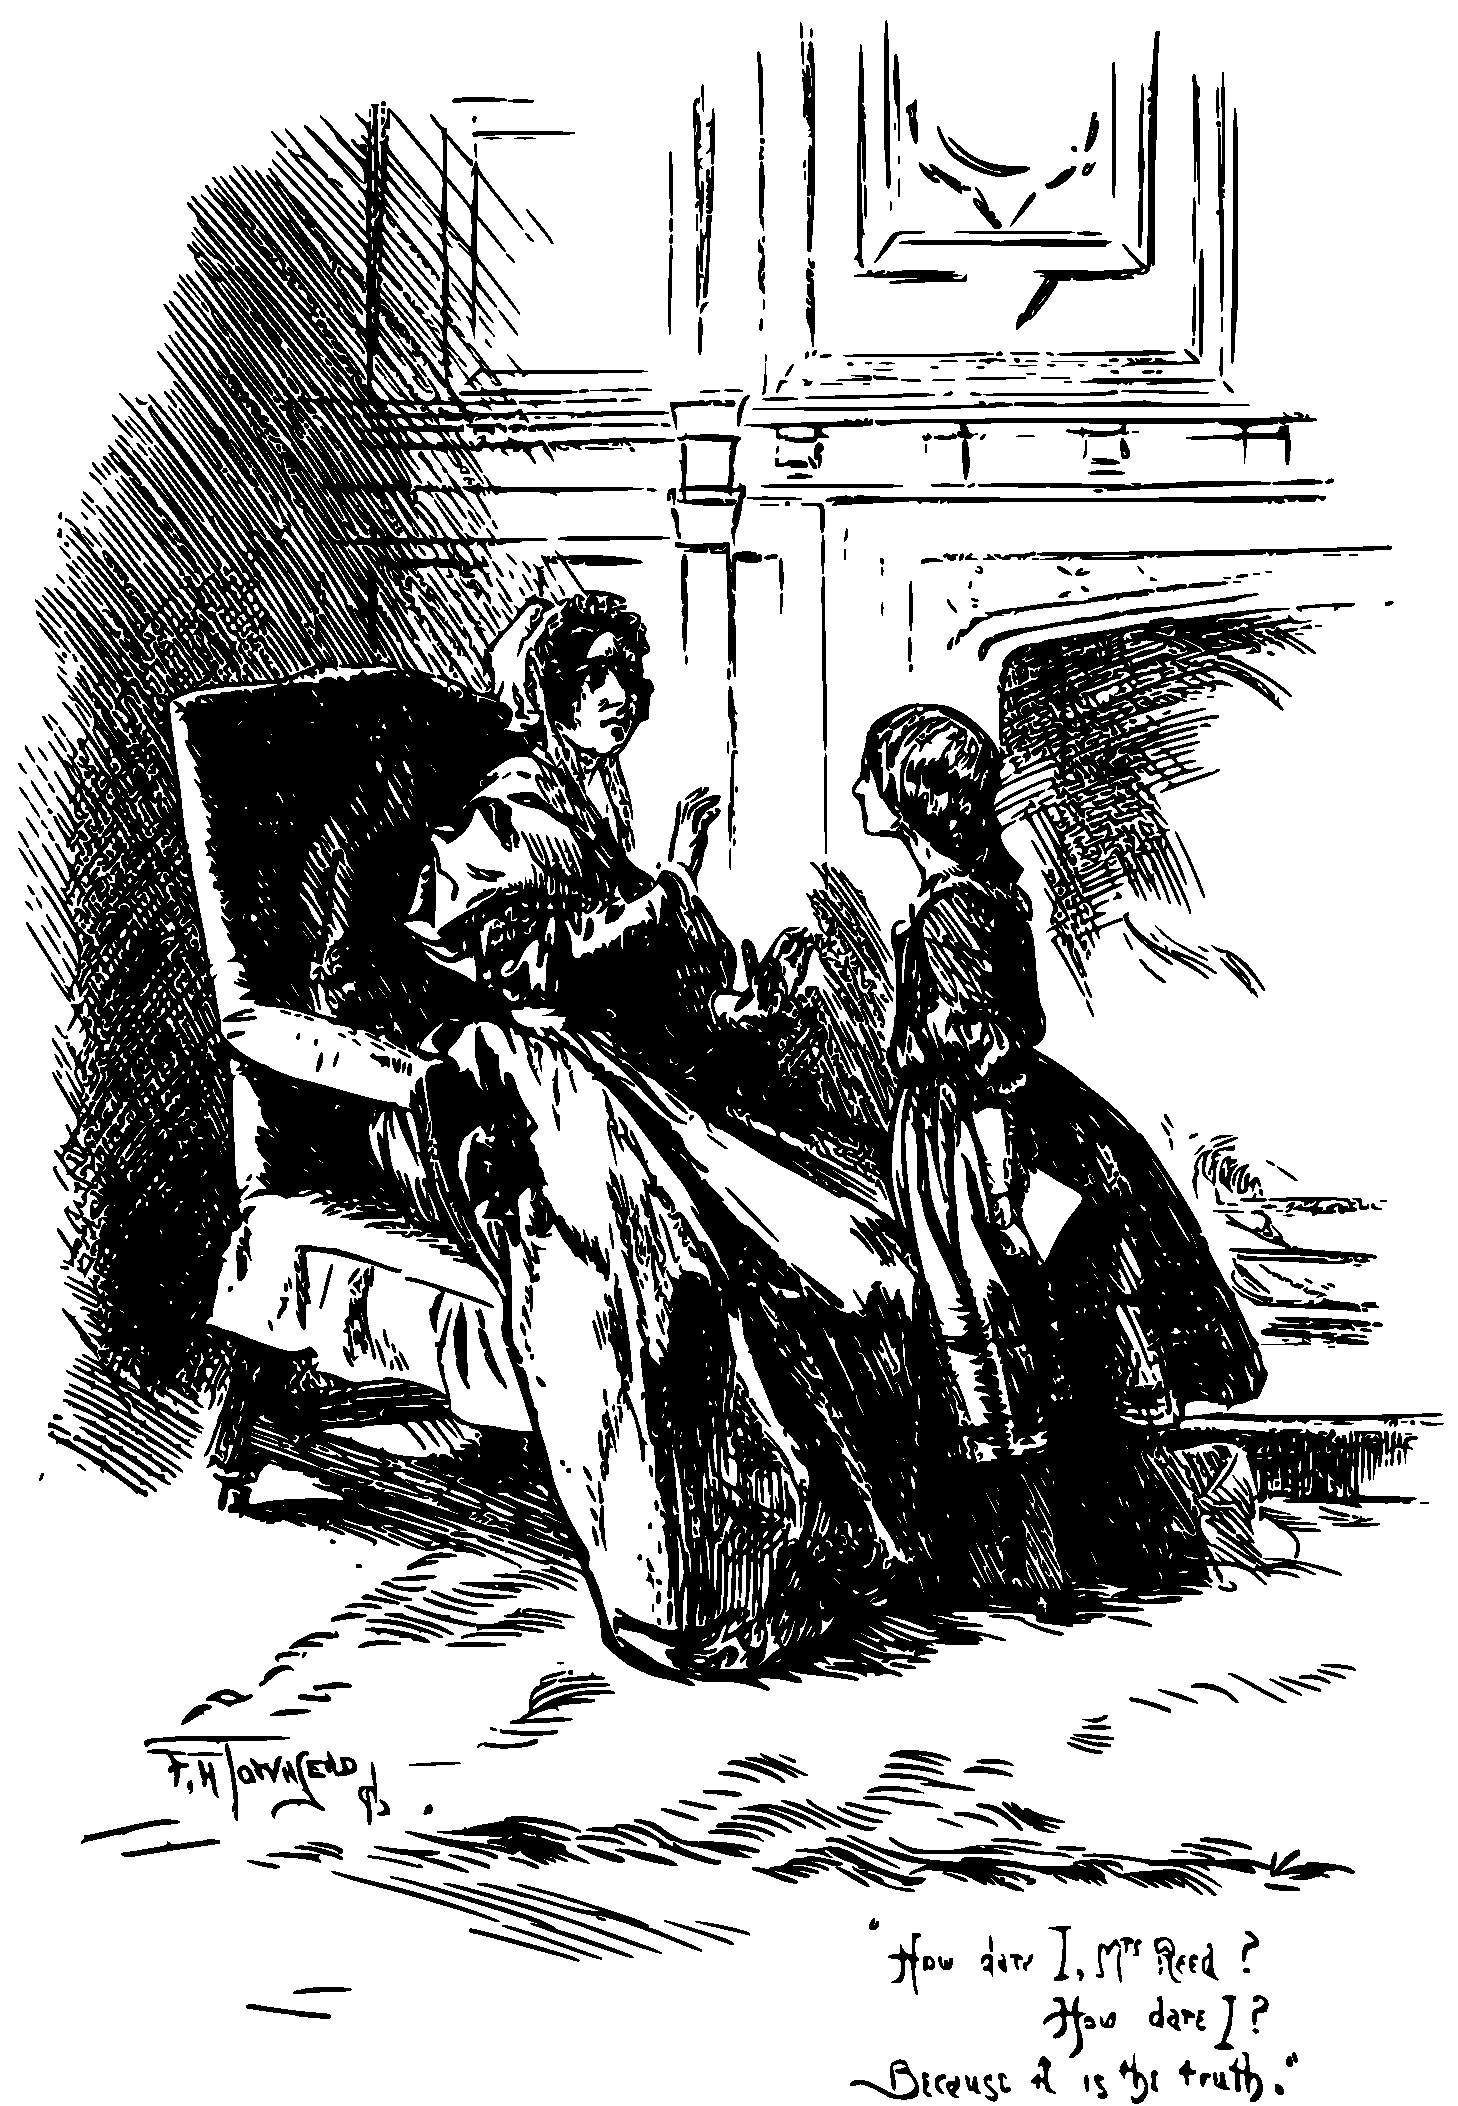
\includegraphics[width=\linewidth]{images/p30b.pdf}
	\end{sidecaption}
\end{figure}

Ere I had finished this reply, my soul began to expand, to exult, with
the strangest sense of freedom, of triumph, I ever felt. It seemed as
if an invisible bond had burst, and that I had struggled out into
unhoped-for liberty. Not without cause was this sentiment: \Mrs{} Reed
looked frightened; her work had slipped from her knee; she was lifting
up her hands, rocking herself to and fro, and even twisting her face as
if she would cry.

\enquote{Jane, you are under a mistake: what is the matter with you? 
Why do you tremble so violently? Would you like to drink some water?}

\enquote{No, \Mrs{} Reed.}

\enquote{Is there anything else you wish for, Jane? I assure you, I
desire to be your friend.}

\enquote{Not you. You told \Mr{} Brocklehurst I had a bad character, a
deceitful disposition; and I'll let everybody at Lowood know what you
are, and what you have done.}

\enquote{Jane, you don't understand these things: children must be
corrected for their faults.}

\enquote{Deceit is not my fault!} I cried out in a savage, high voice.

\enquote{But you are passionate, Jane, that you must allow: and now
return to the nursery---there's a dear---and lie down a little.}

\enquote{I am not your dear; I cannot lie down: send me to school soon,
\Mrs{} Reed, for I hate to live here.}

\enquote{I will indeed send her to school soon,} murmured \Mrs{} Reed
\emph{sotto voce}; and gathering up her work, she abruptly quitted the
apartment.

I was left there alone---winner of the field. It was the hardest battle
I had fought, and the first victory I had gained: I stood awhile on the
rug, where \Mr{} Brocklehurst had stood, and I enjoyed my conqueror's
solitude. First, I smiled to myself and felt elate; but this fierce
pleasure subsided in me as fast as did the accelerated throb of my
pulses. A child cannot quarrel with its elders, as I had done; cannot
give its furious feelings uncontrolled play, as I had given mine,
without experiencing afterwards the pang of remorse and the chill of
reaction. A ridge of lighted heath, alive, glancing, devouring, would
have been a meet emblem of my mind when I accused and menaced \Mrs{} Reed:
the same ridge, black and blasted after the flames are dead, would have
represented as meetly my subsequent condition, when half-an-hour's
silence and reflection had shown me the madness of my conduct, and the
dreariness of my hated and hating position.

Something of vengeance I had tasted for the first time; as aromatic wine
it seemed, on swallowing, warm and racy: its after-flavour, metallic and
corroding, gave me a sensation as if I had been poisoned. Willingly
would I now have gone and asked \Mrs{} Reed's pardon; but I knew, partly
from experience and partly from instinct, that was the way to make her
repulse me with double scorn, thereby re-exciting every turbulent
impulse of my nature.

I would fain exercise some better faculty than that of fierce speaking;
fain find nourishment for some less fiendish feeling than that of sombre
indignation. I took a book---some Arabian tales; I sat down and
endeavoured to read. I could make no sense of the subject; my own
thoughts swam always between me and the page I had usually found
fascinating. I opened the glass-door in the breakfast-room: the
shrubbery was quite still: the black frost reigned, unbroken by sun or
breeze, through the grounds. I covered my head and arms with the skirt
of my frock, and went out to walk in a part of the plantation which was
quite sequestrated; but I found no pleasure in the silent trees, the
falling fir-cones, the congealed relics of autumn, russet leaves, swept
by past winds in heaps, and now stiffened together. I leaned against a
gate, and looked into an empty field where no sheep were feeding, where
the short grass was nipped and blanched. It was a very grey day; a most
opaque sky, \enquote{onding on snaw,} canopied all; thence flakes felt
it intervals, which settled on the hard path and on the hoary lea
without melting. I stood, a wretched child enough, whispering to myself
over and over again, \enquote{What shall I do?---what shall I do?}

All at once I heard a clear voice call, \enquote{Miss Jane! where are
you? Come to lunch!}

It was Bessie, I knew well enough; but I did not stir; her light step
came tripping down the path.

\enquote{You naughty little thing!} she said. \enquote{Why don't you
come when you are called?}

Bessie's presence, compared with the thoughts over which I had been
brooding, seemed cheerful; even though, as usual, she was somewhat
cross. The fact is, after my conflict with and victory over \Mrs{} Reed,
I was not disposed to care much for the nursemaid's transitory anger;
and I \emph{was} disposed to bask in her youthful lightness of heart. I
just put my two arms round her and said, \enquote{Come, Bessie! don't
scold.}

The action was more frank and fearless than any I was habituated to
indulge in: somehow it pleased her.

\enquote{You are a strange child, Miss Jane,} she said, as she looked
down at me; \enquote{a little roving, solitary thing: and you are going
to school, I suppose?}

I nodded.

\enquote{And won't you be sorry to leave poor Bessie?}

\enquote{What does Bessie care for me? She is always scolding me.}

\enquote{Because you're such a queer, frightened, shy little thing. You
should be bolder.}

\enquote{What! to get more knocks?}

\enquote{Nonsense! But you are rather put upon, that's certain. My
mother said, when she came to see me last week, that she would not like
a little one of her own to be in your place.---Now, come in, and I've
some good news for you.}

\enquote{I don't think you have, Bessie.}

\enquote{Child! what do you mean? What sorrowful eyes you fix on me! 
Well, but Missis and the young ladies and Master John are going out to
tea this afternoon, and you shall have tea with me. I'll ask cook to
bake you a little cake, and then you shall help me to look over your
drawers; for I am soon to pack your trunk. Missis intends you to leave
Gateshead in a day or two, and you shall choose what toys you like to
take with you.}

\enquote{Bessie, you must promise not to scold me any more till I go.}

\enquote{Well, I will; but mind you are a very good girl, and don't be
afraid of me. Don't start when I chance to speak rather sharply; it's
so provoking.}

\enquote{I don't think I shall ever be afraid of you again, Bessie,
because I have got used to you, and I shall soon have another set of
people to dread.}

\enquote{If you dread them they'll dislike you.}

\enquote{As you do, Bessie?}

\enquote{I don't dislike you, Miss; I believe I am fonder of you than of
all the others.}

\enquote{You don't show it.}

\enquote{You little sharp thing! you've got quite a new way of talking. 
What makes you so venturesome and hardy?}

\enquote{Why, I shall soon be away from you, and besides}---I was going
to say something about what had passed between me and \Mrs{} Reed, but on
second thoughts I considered it better to remain silent on that head.

\enquote{And so you're glad to leave me?}

\enquote{Not at all, Bessie; indeed, just now I'm rather sorry.}

\enquote{Just now! and rather! How coolly my little lady says it! I dare say
now if I were to ask you for a kiss you wouldn't give it me: you'd say
you'd \emph{rather} not.}

\enquote{I'll kiss you and welcome: bend your head down.} Bessie
stooped; we mutually embraced, and I followed her into the house quite
comforted. That afternoon lapsed in peace and harmony; and in the
evening Bessie told me some of her most enchanting stories, and sang me
some of her sweetest songs. Even for me life had its gleams of
sunshine.

\FChapter{Chapter Five}{5}

\Lettrine{F}{ive} \textsc{o'clock} had hardly struck on the morning of the 19th of January,
when Bessie brought a candle into my closet and found me already up and
nearly dressed. I had risen half-an-hour before her entrance, and had
washed my face, and put on my clothes by the light of a half-moon just
setting, whose rays streamed through the narrow window near my crib. I
was to leave Gateshead that day by a coach which passed the lodge gates
at six \AM{} Bessie was the only person yet risen; she had lit a fire in
the nursery, where she now proceeded to make my breakfast. Few children
can eat when excited with the thoughts of a journey; nor could I\@.
Bessie, having pressed me in vain to take a few spoonfuls of the boiled
milk and bread she had prepared for me, wrapped up some biscuits in a
paper and put them into my bag; then she helped me on with my pelisse
and bonnet, and wrapping herself in a shawl, she and I left the
nursery. As we passed \Mrs{} Reed's bedroom, she said, \enquote{Will you
	go in and bid Missis good-bye?}

\enquote{No, Bessie: she came to my crib last night when you were gone
	down to supper, and said I need not disturb her in the morning, or my
	cousins either; and she told me to remember that she had always been my
	best friend, and to speak of her and be grateful to her accordingly.}

\enquote{What did you say, Miss?}

\enquote{Nothing: I covered my face with the bedclothes, and turned from
	her to the wall.}

\enquote{That was wrong, Miss Jane.}

\enquote{It was quite right, Bessie. Your Missis has not been my
	friend: she has been my foe.}

\enquote{O Miss Jane! don't say so!}

\enquote{Good-bye to Gateshead!} cried I, as we passed through the hall
and went out at the front door.

The moon was set, and it was very dark; Bessie carried a lantern, whose
light glanced on wet steps and gravel road sodden by a recent thaw. Raw
and chill was the winter morning: my teeth chattered as I hastened down
the drive. There was a light in the porter's lodge: when we reached it,
we found the porter's wife just kindling her fire: my trunk, which had
been carried down the evening before, stood corded at the door. It
wanted but a few minutes of six, and shortly after that hour had struck,
the distant roll of wheels announced the coming coach; I went to the
door and watched its lamps approach rapidly through the gloom.

\enquote{Is she going by herself?} asked the porter's wife.

\enquote{Yes.}

\enquote{And how far is it?}

\enquote{Fifty miles.}

\enquote{What a long way! I wonder \Mrs{} Reed is not afraid to trust her
	so far alone.}

The coach drew up; there it was at the gates with its four horses and
its top laden with passengers: the guard and coachman loudly urged
haste; my trunk was hoisted up; I was taken from Bessie's neck, to which
I clung with kisses.

\enquote{Be sure and take good care of her,} cried she to the guard, as
he lifted me into the inside.

\enquote{Ay, ay!} was the answer: the door was slapped to, a voice
exclaimed \enquote{All right,} and on we drove. Thus was I severed from
Bessie and Gateshead; thus whirled away to unknown, and, as I then
deemed, remote and mysterious regions.

I remember but little of the journey; I only know that the day seemed to
me of a preternatural length, and that we appeared to travel over
hundreds of miles of road. We passed through several towns, and in one,
a very large one, the coach stopped; the horses were taken out, and the
passengers alighted to dine. I was carried into an inn, where the guard
wanted me to have some dinner; but, as I had no appetite, he left me in
an immense room with a fireplace at each end, a chandelier pendent from
the ceiling, and a little red gallery high up against the wall filled
with musical instruments. Here I walked about for a long time, feeling
very strange, and mortally apprehensive of some one coming in and
kidnapping me; for I believed in kidnappers, their exploits having
frequently figured in Bessie's fireside chronicles. At last the guard
returned; once more I was stowed away in the coach, my protector mounted
his own seat, sounded his hollow horn, and away we rattled over the
\enquote{stony street} of L-.

The afternoon came on wet and somewhat misty: as it waned into dusk, I
began to feel that we were getting very far indeed from Gateshead: we
ceased to pass through towns; the country changed; great grey hills
heaved up round the horizon: as twilight deepened, we descended a
valley, dark with wood, and long after night had overclouded the
prospect, I heard a wild wind rushing amongst trees.

Lulled by the sound, I at last dropped asleep; I had not long slumbered
when the sudden cessation of motion awoke me; the coach-door was open,
and a person like a servant was standing at it: I saw her face and dress
by the light of the lamps.

\enquote{Is there a little girl called Jane Eyre here?} she asked. I
answered \enquote{Yes,} and was then lifted out; my trunk was handed
down, and the coach instantly drove away.

I was stiff with long sitting, and bewildered with the noise and motion
of the coach: Gathering my faculties, I looked about me. Rain, wind,
and darkness filled the air; nevertheless, I dimly discerned a wall
before me and a door open in it; through this door I passed with my new
guide: she shut and locked it behind her. There was now visible a house
or houses---for the building spread far---with many windows, and lights
burning in some; we went up a broad pebbly path, splashing wet, and were
admitted at a door; then the servant led me through a passage into a
room with a fire, where she left me alone.

I stood and warmed my numbed fingers over the blaze, then I looked
round; there was no candle, but the uncertain light from the hearth
showed, by intervals, papered walls, carpet, curtains, shining mahogany
furniture: it was a parlour, not so spacious or splendid as the
drawing-room at Gateshead, but comfortable enough. I was puzzling to
make out the subject of a picture on the wall, when the door opened, and
an individual carrying a light entered; another followed close behind.

The first was a tall lady with dark hair, dark eyes, and a pale and
large forehead; her figure was partly enveloped in a shawl, her
countenance was grave, her bearing erect.

\enquote{The child is very young to be sent alone,} said she, putting
her candle down on the table. She considered me attentively for a
minute or two, then further added---

\enquote{She had better be put to bed soon; she looks tired: are you
	tired?} she asked, placing her hand on my shoulder.

\enquote{A little, ma'am.}

\enquote{And hungry too, no doubt: let her have some supper before she
	goes to bed, Miss Miller. Is this the first time you have left your
	parents to come to school, my little girl?}

I explained to her that I had no parents. She inquired how long they
had been dead: then how old I was, what was my name, whether I could
read, write, and sew a little: then she touched my cheek gently with her
forefinger, and saying, \enquote{She hoped I should be a good child,}
dismissed me along with Miss Miller.

The lady I had left might be about twenty-nine; the one who went with me
appeared some years younger: the first impressed me by her voice, look,
and air. Miss Miller was more ordinary; ruddy in complexion, though of
a careworn countenance; hurried in gait and action, like one who had
always a multiplicity of tasks on hand: she looked, indeed, what I
afterwards found she really was, an under-teacher. Led by her, I passed
from compartment to compartment, from passage to passage, of a large and
irregular building; till, emerging from the total and somewhat dreary
silence pervading that portion of the house we had traversed, we came
upon the hum of many voices, and presently entered a wide, long room,
with great deal tables, two at each end, on each of which burnt a pair
of candles, and seated all round on benches, a congregation of girls of
every age, from nine or ten to twenty. Seen by the dim light of the
dips, their number to me appeared countless, though not in reality
exceeding eighty; they were uniformly dressed in brown stuff frocks of
quaint fashion, and long holland pinafores. It was the hour of study;
they were engaged in conning over their to-morrow's task, and the hum I
had heard was the combined result of their whispered repetitions.

Miss Miller signed to me to sit on a bench near the door, then walking
up to the top of the long room she cried out---

\enquote{Monitors, collect the lesson-books and put them away!}

Four tall girls arose from different tables, and going round, gathered
the books and removed them. Miss Miller again gave the word of
command---

\enquote{Monitors, fetch the supper-trays!}

The tall girls went out and returned presently, each bearing a tray,
with portions of something, I knew not what, arranged thereon, and a
pitcher of water and mug in the middle of each tray. The portions were
handed round; those who liked took a draught of the water, the mug being
common to all. When it came to my turn, I drank, for I was thirsty, but
did not touch the food, excitement and fatigue rendering me incapable of
eating: I now saw, however, that it was a thin oaten cake shared into
fragments.

The meal over, prayers were read by Miss Miller, and the classes filed
off, two and two, upstairs. Overpowered by this time with weariness, I
scarcely noticed what sort of a place the bedroom was, except that, like
the schoolroom, I saw it was very long. To-night I was to be Miss
Miller's bed-fellow; she helped me to undress: when laid down I glanced
at the long rows of beds, each of which was quickly filled with two
occupants; in ten minutes the single light was extinguished, and amidst
silence and complete darkness I fell asleep.

The night passed rapidly. I was too tired even to dream; I only once
awoke to hear the wind rave in furious gusts, and the rain fall in
torrents, and to be sensible that Miss Miller had taken her place by my
side. When I again unclosed my eyes, a loud bell was ringing; the girls
were up and dressing; day had not yet begun to dawn, and a rushlight or
two burned in the room. I too rose reluctantly; it was bitter cold, and
I dressed as well as I could for shivering, and washed when there was a
basin at liberty, which did not occur soon, as there was but one basin
to six girls, on the stands down the middle of the room. Again the bell
rang: all formed in file, two and two, and in that order descended the
stairs and entered the cold and dimly lit schoolroom: here prayers were
read by Miss Miller; afterwards she called out---

\enquote{Form classes!}

A great tumult succeeded for some minutes, during which Miss Miller
repeatedly exclaimed, \enquote{Silence!} and \enquote{Order!} When it
subsided, I saw them all drawn up in four semicircles, before four
chairs, placed at the four tables; all held books in their hands, and a
great book, like a Bible, lay on each table, before the vacant seat. A
pause of some seconds succeeded, filled up by the low, vague hum of
numbers; Miss Miller walked from class to class, hushing this indefinite
sound.

A distant bell tinkled: immediately three ladies entered the room, each
walked to a table and took her seat. Miss Miller assumed the fourth
vacant chair, which was that nearest the door, and around which the
smallest of the children were assembled: to this inferior class I was
called, and placed at the bottom of it.

Business now began, the day's Collect was repeated, then certain texts
of Scripture were said, and to these succeeded a protracted reading of
chapters in the Bible, which lasted an hour. By the time that exercise
was terminated, day had fully dawned. The indefatigable bell now
sounded for the fourth time: the classes were marshalled and marched
into another room to breakfast: how glad I was to behold a prospect of
getting something to eat! I was now nearly sick from inanition, having
taken so little the day before.

The refectory was a great, low-ceiled, gloomy room; on two long tables
smoked basins of something hot, which, however, to my dismay, sent forth
an odour far from inviting. I saw a universal manifestation of
discontent when the fumes of the repast met the nostrils of those
destined to swallow it; from the van of the procession, the tall girls
of the first class, rose the whispered words---

\enquote{Disgusting! The porridge is burnt again!}

\enquote{Silence!} ejaculated a voice; not that of Miss Miller, but one
of the upper teachers, a little and dark personage, smartly dressed, but
of somewhat morose aspect, who installed herself at the top of one
table, while a more buxom lady presided at the other. I looked in vain
for her I had first seen the night before; she was not visible: Miss
Miller occupied the foot of the table where I sat, and a strange,
foreign-looking, elderly lady, the French teacher, as I afterwards
found, took the corresponding seat at the other board. A long grace was
said and a hymn sung; then a servant brought in some tea for the
teachers, and the meal began.

Ravenous, and now very faint, I devoured a spoonful or two of my portion
without thinking of its taste; but the first edge of hunger blunted, I
perceived I had got in hand a nauseous mess; burnt porridge is almost as
bad as rotten potatoes; famine itself soon sickens over it. The spoons
were moved slowly: I saw each girl taste her food and try to swallow it;
but in most cases the effort was soon relinquished. Breakfast was over,
and none had breakfasted. Thanks being returned for what we had not
got, and a second hymn chanted, the refectory was evacuated for the
schoolroom. I was one of the last to go out, and in passing the tables,
I saw one teacher take a basin of the porridge and taste it; she looked
at the others; all their countenances expressed displeasure, and one of
them, the stout one, whispered---

\enquote{Abominable stuff! How shameful!}

A quarter of an hour passed before lessons again began, during which the
schoolroom was in a glorious tumult; for that space of time it seemed to
be permitted to talk loud and more freely, and they used their
privilege. The whole conversation ran on the breakfast, which one and
all abused roundly. Poor things! it was the sole consolation they had.
Miss Miller was now the only teacher in the room: a group of great girls
standing about her spoke with serious and sullen gestures. I heard the
name of \Mr{} Brocklehurst pronounced by some lips; at which Miss Miller
shook her head disapprovingly; but she made no great effort to check the
general wrath; doubtless she shared in it.

A clock in the schoolroom struck nine; Miss Miller left her circle, and
standing in the middle of the room, cried---

\enquote{Silence! To your seats!}

Discipline prevailed: in five minutes the confused throng was resolved
into order, and comparative silence quelled the Babel clamour of
tongues. The upper teachers now punctually resumed their posts: but
still, all seemed to wait. Ranged on benches down the sides of the
room, the eighty girls sat motionless and erect; a quaint assemblage
they appeared, all with plain locks combed from their faces, not a curl
visible; in brown dresses, made high and surrounded by a narrow tucker
about the throat, with little pockets of holland (shaped something like
a Highlander's purse) tied in front of their frocks, and destined to
serve the purpose of a work-bag: all, too, wearing woollen stockings and
country-made shoes, fastened with brass buckles. Above twenty of those
clad in this costume were full-grown girls, or rather young women; it
suited them ill, and gave an air of oddity even to the prettiest.

I was still looking at them, and also at intervals examining the
teachers---none of whom precisely pleased me; for the stout one was a
little coarse, the dark one not a little fierce, the foreigner harsh and
grotesque, and Miss Miller, poor thing! looked purple, weather-beaten,
and over-worked---when, as my eye wandered from face to face, the whole
school rose simultaneously, as if moved by a common spring.

What was the matter? I had heard no order given: I was puzzled. Ere I
had gathered my wits, the classes were again seated: but as all eyes
were now turned to one point, mine followed the general direction, and
encountered the personage who had received me last night. She stood at
the bottom of the long room, on the hearth; for there was a fire at each
end; she surveyed the two rows of girls silently and gravely. Miss
Miller approaching, seemed to ask her a question, and having received
her answer, went back to her place, and said aloud---

\enquote{Monitor of the first class, fetch the globes!}

While the direction was being executed, the lady consulted moved slowly
up the room. I suppose I have a considerable organ of veneration, for I
retain yet the sense of admiring awe with which my eyes traced her
steps. Seen now, in broad daylight, she looked tall, fair, and shapely;
brown eyes with a benignant light in their irids, and a fine pencilling
of long lashes round, relieved the whiteness of her large front; on each
of her temples her hair, of a very dark brown, was clustered in round
curls, according to the fashion of those times, when neither smooth
bands nor long ringlets were in vogue; her dress, also in the mode of
the day, was of purple cloth, relieved by a sort of Spanish trimming of
black velvet; a gold watch (watches were not so common then as now)
shone at her girdle. Let the reader add, to complete the picture,
refined features; a complexion, if pale, clear; and a stately air and
carriage, and he will have, at least, as clearly as words can give it, a
correct idea of the exterior of Miss Temple---Maria Temple, as I
afterwards saw the name written in a prayer-book intrusted to me to
carry to church.

The superintendent of Lowood (for such was this lady) having taken her
seat before a pair of globes placed on one of the tables, summoned the
first class round her, and commenced giving a lesson on geography; the
lower classes were called by the teachers: repetitions in history,
grammar, \etc, went on for an hour; writing and arithmetic succeeded,
and music lessons were given by Miss Temple to some of the elder girls.
The duration of each lesson was measured by the clock, which at last
struck twelve. The superintendent rose---

\enquote{I have a word to address to the pupils,} said she.

The tumult of cessation from lessons was already breaking forth, but it
sank at her voice. She went on---

\enquote{You had this morning a breakfast which you could not eat; you
	must be hungry:---I have ordered that a lunch of bread and cheese shall
	be served to all.}

The teachers looked at her with a sort of surprise.

\enquote{It is to be done on my responsibility,} she added, in an
explanatory tone to them, and immediately afterwards left the room.

The bread and cheese was presently brought in and distributed, to the
high delight and refreshment of the whole school. The order was now
given \enquote{To the garden!} Each put on a coarse straw bonnet, with
strings of coloured calico, and a cloak of grey frieze. I was similarly
equipped, and, following the stream, I made my way into the open air.

The garden was a wide inclosure, surrounded with walls so high as to
exclude every glimpse of prospect; a covered verandah ran down one side,
and broad walks bordered a middle space divided into scores of little
beds: these beds were assigned as gardens for the pupils to cultivate,
and each bed had an owner. When full of flowers they would doubtless
look pretty; but now, at the latter end of January, all was wintry
blight and brown decay. I shuddered as I stood and looked round me: it
was an inclement day for outdoor exercise; not positively rainy, but
darkened by a drizzling yellow fog; all under foot was still soaking wet
with the floods of yesterday. The stronger among the girls ran about
and engaged in active games, but sundry pale and thin ones herded
together for shelter and warmth in the verandah; and amongst these, as
the dense mist penetrated to their shivering frames, I heard frequently
the sound of a hollow cough.

As yet I had spoken to no one, nor did anybody seem to take notice of
me; I stood lonely enough: but to that feeling of isolation I was
accustomed; it did not oppress me much. I leant against a pillar of the
verandah, drew my grey mantle close about me, and, trying to forget the
cold which nipped me without, and the unsatisfied hunger which gnawed me
within, delivered myself up to the employment of watching and thinking.
My reflections were too undefined and fragmentary to merit record: I
hardly yet knew where I was; Gateshead and my past life seemed floated
away to an immeasurable distance; the present was vague and strange, and
of the future I could form no conjecture. I looked round the
convent-like garden, and then up at the house---a large building, half
of which seemed grey and old, the other half quite new. The new part,
containing the schoolroom and dormitory, was lit by mullioned and
latticed windows, which gave it a church-like aspect; a stone tablet
over the door bore this inscription:---

\enquote{Lowood Institution.---This portion was rebuilt \AD{} ---, by
	Naomi Brocklehurst, of Brocklehurst Hall, in this county.} \enquote{Let
	your light so shine before men, that they may see your good works, and
	glorify your Father which is in heaven.}---\St{} Matt.\@ v.\@ 16.

I read these words over and over again: I felt that an explanation
belonged to them, and was unable fully to penetrate their import. I was
still pondering the signification of \enquote{Institution,} and
endeavouring to make out a connection between the first words and the
verse of Scripture, when the sound of a cough close behind me made me
turn my head. I saw a girl sitting on a stone bench near; she was bent
over a book, on the perusal of which she seemed intent: from where I
stood I could see the title---it was \enquote{Rasselas;} a name that
struck me as strange, and consequently attractive. In turning a leaf
she happened to look up, and I said to her directly---

\enquote{Is your book interesting?} I had already formed the intention
of asking her to lend it to me some day.

\enquote{I like it,} she answered, after a pause of a second or two,
during which she examined me.

\enquote{What is it about?} I continued. I hardly know where I found
the hardihood thus to open a conversation with a stranger; the step was
contrary to my nature and habits: but I think her occupation touched a
chord of sympathy somewhere; for I too liked reading, though of a
frivolous and childish kind; I could not digest or comprehend the
serious or substantial.

\enquote{You may look at it,} replied the girl, offering me the book.

I did so; a brief examination convinced me that the contents were less
taking than the title: \enquote{Rasselas} looked dull to my trifling
taste; I saw nothing about fairies, nothing about genii; no bright
variety seemed spread over the closely-printed pages. I returned it to
her; she received it quietly, and without saying anything she was about
to relapse into her former studious mood: again I ventured to disturb
her---

\enquote{Can you tell me what the writing on that stone over the door
	means? What is Lowood Institution?}

\enquote{This house where you are come to live.}

\enquote{And why do they call it Institution? Is it in any way
	different from other schools?}

\enquote{It is partly a charity-school: you and I, and all the rest of
	us, are charity-children. I suppose you are an orphan: are not either
	your father or your mother dead?}

\enquote{Both died before I can remember.}

\enquote{Well, all the girls here have lost either one or both parents,
	and this is called an institution for educating orphans.}

\enquote{Do we pay no money? Do they keep us for nothing?}

\enquote{We pay, or our friends pay, fifteen pounds a year for each.}

\enquote{Then why do they call us charity-children?}

\enquote{Because fifteen pounds is not enough for board and teaching,
	and the deficiency is supplied by subscription.}

\enquote{Who subscribes?}

\enquote{Different benevolent-minded ladies and gentlemen in this
	neighbourhood and in London.}

\enquote{Who was Naomi Brocklehurst?}

\enquote{The lady who built the new part of this house as that tablet
	records, and whose son overlooks and directs everything here.}

\enquote{Why?}

\enquote{Because he is treasurer and manager of the establishment.}

\enquote{Then this house does not belong to that tall lady who wears a
	watch, and who said we were to have some bread and cheese?}

\enquote{To Miss Temple? Oh, no! I wish it did: she has to answer to
	\Mr{} Brocklehurst for all she does. \Mr{} Brocklehurst buys all our food
	and all our clothes.}

\enquote{Does he live here?}

\enquote{No---two miles off, at a large hall.}

\enquote{Is he a good man?}

\enquote{He is a clergyman, and is said to do a great deal of good.}

\enquote{Did you say that tall lady was called Miss Temple?}

\enquote{Yes.}

\enquote{And what are the other teachers called?}

\enquote{The one with red cheeks is called Miss Smith; she attends to
	the work, and cuts out---for we make our own clothes, our frocks, and
	pelisses, and everything; the little one with black hair is Miss
	Scatcherd; she teaches history and grammar, and hears the second class
	repetitions; and the one who wears a shawl, and has a
	pocket-handkerchief tied to her side with a yellow ribband, is Madame
	Pierrot: she comes from Lisle, in France, and teaches French.}

\enquote{Do you like the teachers?}

\enquote{Well enough.}

\enquote{Do you like the little black one, and the Madame ---?---I
	cannot pronounce her name as you do.}

\enquote{Miss Scatcherd is hasty---you must take care not to offend her;
	Madame Pierrot is not a bad sort of person.}

\enquote{But Miss Temple is the best---isn't she?}

\enquote{Miss Temple is very good and very clever; she is above the
	rest, because she knows far more than they do.}

\enquote{Have you been long here?}

\enquote{Two years.}

\enquote{Are you an orphan?}

\enquote{My mother is dead.}

\enquote{Are you happy here?}

\enquote{You ask rather too many questions. I have given you answers
	enough for the present: now I want to read.}

But at that moment the summons sounded for dinner; all re-entered the
house. The odour which now filled the refectory was scarcely more
appetising than that which had regaled our nostrils at breakfast: the
dinner was served in two huge tin-plated vessels, whence rose a strong
steam redolent of rancid fat. I found the mess to consist of
indifferent potatoes and strange shreds of rusty meat, mixed and cooked
together. Of this preparation a tolerably abundant plateful was
apportioned to each pupil. I ate what I could, and wondered within
myself whether every day's fare would be like this.

After dinner, we immediately adjourned to the schoolroom: lessons
recommenced, and were continued till five o'clock.

The only marked event of the afternoon was, that I saw the girl with
whom I had conversed in the verandah dismissed in disgrace by Miss
Scatcherd from a history class, and sent to stand in the middle of the
large schoolroom. The punishment seemed to me in a high degree
ignominious, especially for so great a girl---she looked thirteen or
upwards. I expected she would show signs of great distress and shame;
but to my surprise she neither wept nor blushed: composed, though grave,
she stood, the central mark of all eyes. \enquote{How can she bear it
	so quietly---so firmly?} I asked of myself. \enquote{Were I in her
	place, it seems to me I should wish the earth to open and swallow me
	up. She looks as if she were thinking of something beyond her
	punishment---beyond her situation: of something not round her nor before
	her. I have heard of day-dreams---is she in a day-dream now? Her eyes
	are fixed on the floor, but I am sure they do not see it---her sight
	seems turned in, gone down into her heart: she is looking at what she
	can remember, I believe; not at what is really present. I wonder what
	sort of a girl she is---whether good or naughty.}

Soon after five \PM{} we had another meal, consisting of a small mug of
coffee, and half-a-slice of brown bread. I devoured my bread and drank
my coffee with relish; but I should have been glad of as much more---I
was still hungry. Half-an-hour's recreation succeeded, then study; then
the glass of water and the piece of oat-cake, prayers, and bed. Such
was my first day at Lowood.

\FChapter{Chapter Six}{6}

\Lettrine{T}{he} \textsc{next day} commenced as before, getting up and dressing by rushlight;
but this morning we were obliged to dispense with the ceremony of
washing; the water in the pitchers was frozen.  A change had taken place
in the weather the preceding evening, and a keen north-east wind,
whistling through the crevices of our bedroom windows all night long,
had made us shiver in our beds, and turned the contents of the ewers to
ice.

Before the long hour and a half of prayers and Bible-reading was over, I
felt ready to perish with cold.  Breakfast-time came at last, and this
morning the porridge was not burnt; the quality was eatable, the
quantity small.  How small my portion seemed!  I wished it had been
doubled.

In the course of the day I was enrolled a member of the fourth class,
and regular tasks and occupations were assigned me: hitherto, I had only
been a spectator of the proceedings at Lowood; I was now to become an
actor therein.  At first, being little accustomed to learn by heart, the
lessons appeared to me both long and difficult; the frequent change from
task to task, too, bewildered me; and I was glad when, about three
o'clock in the afternoon, Miss Smith put into my hands a border of
muslin two yards long, together with needle, thimble, \etc, and sent me
to sit in a quiet corner of the schoolroom, with directions to hem the
same.  At that hour most of the others were sewing likewise; but one
class still stood round Miss Scatcherd's chair reading, and as all was
quiet, the subject of their lessons could be heard, together with the
manner in which each girl acquitted herself, and the animadversions or
commendations of Miss Scatcherd on the performance.  It was English
history: among the readers I observed my acquaintance of the verandah:
at the commencement of the lesson, her place had been at the top of the
class, but for some error of pronunciation, or some inattention to
stops, she was suddenly sent to the very bottom.  Even in that obscure
position, Miss Scatcherd continued to make her an object of constant
notice: she was continually addressing to her such phrases as the
following:---

\enquote{Burns} (such it seems was her name: the girls here were all
called by their surnames, as boys are elsewhere), \enquote{Burns, you
	are standing on the side of your shoe; turn your toes out immediately.}
\enquote{Burns, you poke your chin most unpleasantly; draw it in.}
\enquote{Burns, I insist on your holding your head up; I will not have
	you before me in that attitude,} \etc{} \etc.

A chapter having been read through twice, the books were closed and the
girls examined.  The lesson had comprised part of the reign of Charles
I., and there were sundry questions about tonnage and poundage and
ship-money, which most of them appeared unable to answer; still, every
little difficulty was solved instantly when it reached Burns: her memory
seemed to have retained the substance of the whole lesson, and she was
ready with answers on every point.  I kept expecting that Miss Scatcherd
would praise her attention; but, instead of that, she suddenly cried
out---

\enquote{You dirty, disagreeable girl! you have never cleaned your nails
	this morning!}

Burns made no answer: I wondered at her silence.  \enquote{Why,} thought
I, \enquote{does she not explain that she could neither clean her nails
	nor wash her face, as the water was frozen?}

My attention was now called off by Miss Smith desiring me to hold a
skein of thread: while she was winding it, she talked to me from time to
time, asking whether I had ever been at school before, whether I could
mark, stitch, knit, \etc; till she dismissed me, I could not pursue my
observations on Miss Scatcherd's movements.  When I returned to my seat,
that lady was just delivering an order of which I did not catch the
import; but Burns immediately left the class, and going into the small
inner room where the books were kept, returned in half a minute,
carrying in her hand a bundle of twigs tied together at one end.  This
ominous tool she presented to Miss Scatcherd with a respectful curtesy;
then she quietly, and without being told, unloosed her pinafore, and the
teacher instantly and sharply inflicted on her neck a dozen strokes with
the bunch of twigs.  Not a tear rose to Burns' eye; and, while I paused
from my sewing, because my fingers quivered at this spectacle with a
sentiment of unavailing and impotent anger, not a feature of her pensive
face altered its ordinary expression.

\enquote{Hardened girl!} exclaimed Miss Scatcherd; \enquote{nothing can
	correct you of your slatternly habits: carry the rod away.}

Burns obeyed: I looked at her narrowly as she emerged from the
book-closet; she was just putting back her handkerchief into her pocket,
and the trace of a tear glistened on her thin cheek.

The play-hour in the evening I thought the pleasantest fraction of the
day at Lowood: the bit of bread, the draught of coffee swallowed at five
o'clock had revived vitality, if it had not satisfied hunger: the long
restraint of the day was slackened; the schoolroom felt warmer than in
the morning---its fires being allowed to burn a little more brightly, to
supply, in some measure, the place of candles, not yet introduced: the
ruddy gloaming, the licensed uproar, the confusion of many voices gave
one a welcome sense of liberty.

On the evening of the day on which I had seen Miss Scatcherd flog her
pupil, Burns, I wandered as usual among the forms and tables and
laughing groups without a companion, yet not feeling lonely: when I
passed the windows, I now and then lifted a blind, and looked out; it
snowed fast, a drift was already forming against the lower panes;
putting my ear close to the window, I could distinguish from the gleeful
tumult within, the disconsolate moan of the wind outside.

Probably, if I had lately left a good home and kind parents, this would
have been the hour when I should most keenly have regretted the
separation; that wind would then have saddened my heart; this obscure
chaos would have disturbed my peace! as it was, I derived from both a
strange excitement, and reckless and feverish, I wished the wind to howl
more wildly, the gloom to deepen to darkness, and the confusion to rise
to clamour.

Jumping over forms, and creeping under tables, I made my way to one of
the fire-places; there, kneeling by the high wire fender, I found Burns,
absorbed, silent, abstracted from all round her by the companionship of
a book, which she read by the dim glare of the embers.

\enquote{Is it still \enquote{Rasselas}?} I asked, coming behind her.

\enquote{Yes,} she said, \enquote{and I have just finished it.}

And in five minutes more she shut it up.  I was glad of this.
\enquote{Now,} thought I, \enquote{I can perhaps get her to talk.}  I
sat down by her on the floor.

\enquote{What is your name besides Burns?}

\enquote{Helen.}

\enquote{Do you come a long way from here?}

\enquote{I come from a place farther north, quite on the borders of
	Scotland.}

\enquote{Will you ever go back?}

\enquote{I hope so; but nobody can be sure of the future.}

\enquote{You must wish to leave Lowood?}

\enquote{No! why should I?  I was sent to Lowood to get an education;
	and it would be of no use going away until I have attained that object.}

\enquote{But that teacher, Miss Scatcherd, is so cruel to you?}

\enquote{Cruel?  Not at all!  She is severe: she dislikes my faults.}

\enquote{And if I were in your place I should dislike her; I should
	resist her.  If she struck me with that rod, I should get it from her
	hand; I should break it under her nose.}

\enquote{Probably you would do nothing of the sort: but if you did, \Mr{}
	Brocklehurst would expel you from the school; that would be a great
	grief to your relations.  It is far better to endure patiently a smart
	which nobody feels but yourself, than to commit a hasty action whose
	evil consequences will extend to all connected with you; and besides,
	the Bible bids us return good for evil.}

\enquote{But then it seems disgraceful to be flogged, and to be sent to
	stand in the middle of a room full of people; and you are such a great
	girl: I am far younger than you, and I could not bear it.}

\enquote{Yet it would be your duty to bear it, if you could not avoid it: it is
	weak and silly to say you \emph{cannot bear} what it is your fate to be
	required to bear.}

I heard her with wonder: I could not comprehend this doctrine of
endurance; and still less could I understand or sympathise with the
forbearance she expressed for her chastiser.  Still I felt that Helen
Burns considered things by a light invisible to my eyes.  I suspected
she might be right and I wrong; but I would not ponder the matter
deeply; like Felix, I put it off to a more convenient season.

\enquote{You say you have faults, Helen: what are they?  To me you seem
	very good.}

\enquote{Then learn from me, not to judge by appearances: I am, as Miss
	Scatcherd said, slatternly; I seldom put, and never keep, things, in
	order; I am careless; I forget rules; I read when I should learn my
	lessons; I have no method; and sometimes I say, like you, I cannot
	\emph{bear} to be subjected to systematic arrangements.  This is all
	very provoking to Miss Scatcherd, who is naturally neat, punctual, and
	particular.}

\enquote{And cross and cruel,} I added; but Helen Burns would not admit
my addition: she kept silence.

\enquote{Is Miss Temple as severe to you as Miss Scatcherd?}

At the utterance of Miss Temple's name, a soft smile flitted over her
grave face.

\enquote{Miss Temple is full of goodness; it pains her to be severe to
	any one, even the worst in the school: she sees my errors, and tells me
	of them gently; and, if I do anything worthy of praise, she gives me my
	meed liberally.  One strong proof of my wretchedly defective nature is,
	that even her expostulations, so mild, so rational, have not influence
	to cure me of my faults; and even her praise, though I value it most
	highly, cannot stimulate me to continued care and foresight.}

\enquote{That is curious,} said I, \enquote{it is so easy to be
	careful.}

\enquote{For \emph{you} I have no doubt it is.  I observed you in your class
	this morning, and saw you were closely attentive: your thoughts never
	seemed to wander while Miss Miller explained the lesson and questioned
	you.  Now, mine continually rove away; when I should be listening to
	Miss Scatcherd, and collecting all she says with assiduity, often I lose
	the very sound of her voice; I fall into a sort of dream.  Sometimes I
	think I am in Northumberland, and that the noises I hear round me are
	the bubbling of a little brook which runs through Deepden, near our
	house;---then, when it comes to my turn to reply, I have to be awakened;
	and having heard nothing of what was read for listening to the visionary
	brook, I have no answer ready.}

\enquote{Yet how well you replied this afternoon.}

\enquote{It was mere chance; the subject on which we had been reading
	had interested me.  This afternoon, instead of dreaming of Deepden, I
	was wondering how a man who wished to do right could act so unjustly and
	unwisely as Charles the First sometimes did; and I thought what a pity
	it was that, with his integrity and conscientiousness, he could see no
	farther than the prerogatives of the crown.  If he had but been able to
	look to a distance, and see how what they call the spirit of the age was
	tending!  Still, I like Charles---I respect him---I pity him, poor
	murdered king!  Yes, his enemies were the worst: they shed blood they
	had no right to shed.  How dared they kill him!}

Helen was talking to herself now: she had forgotten I could not very
well understand her---that I was ignorant, or nearly so, of the subject
she discussed.  I recalled her to my level.

\enquote{And when Miss Temple teaches you, do your thoughts wander
	then?}

\enquote{No, certainly, not often; because Miss Temple has generally
	something to say which is newer than my own reflections; her language is
	singularly agreeable to me, and the information she communicates is
	often just what I wished to gain.}

\enquote{Well, then, with Miss Temple you are good?}

\enquote{Yes, in a passive way: I make no effort; I follow as
	inclination guides me.  There is no merit in such goodness.}

\enquote{A great deal: you are good to those who are good to you.  It is
	all I ever desire to be.  If people were always kind and obedient to
	those who are cruel and unjust, the wicked people would have it all
	their own way: they would never feel afraid, and so they would never
	alter, but would grow worse and worse.  When we are struck at without a
	reason, we should strike back again very hard; I am sure we should---so
	hard as to teach the person who struck us never to do it again.}

\enquote{You will change your mind, I hope, when you grow older: as yet
	you are but a little untaught girl.}

\enquote{But I feel this, Helen; I must dislike those who, whatever I do
	to please them, persist in disliking me; I must resist those who punish
	me unjustly.  It is as natural as that I should love those who show me
	affection, or submit to punishment when I feel it is deserved.}

\enquote{Heathens and savage tribes hold that doctrine, but Christians
	and civilised nations disown it.}

\enquote{How?  I don't understand.}

\enquote{It is not violence that best overcomes hate---nor vengeance
	that most certainly heals injury.}

\enquote{What then?}

\enquote{Read the New Testament, and observe what Christ says, and how
	He acts; make His word your rule, and His conduct your example.}

\enquote{What does He say?}

\enquote{Love your enemies; bless them that curse you; do good to them
	that hate you and despitefully use you.}

\enquote{Then I should love \Mrs{} Reed, which I cannot do; I should bless
	her son John, which is impossible.}

In her turn, Helen Burns asked me to explain, and I proceeded forthwith
to pour out, in my own way, the tale of my sufferings and resentments.
Bitter and truculent when excited, I spoke as I felt, without reserve or
softening.

Helen heard me patiently to the end: I expected she would then make a
remark, but she said nothing.

\enquote{Well,} I asked impatiently, \enquote{is not \Mrs{} Reed a
	hard-hearted, bad woman?}

\enquote{She has been unkind to you, no doubt; because you see, she
	dislikes your cast of character, as Miss Scatcherd does mine; but how
	minutely you remember all she has done and said to you!  What a
	singularly deep impression her injustice seems to have made on your
	heart!  No ill-usage so brands its record on my feelings.  Would you not
	be happier if you tried to forget her severity, together with the
	passionate emotions it excited?  Life appears to me too short to be
	spent in nursing animosity or registering wrongs.  We are, and must be,
	one and all, burdened with faults in this world: but the time will soon
	come when, I trust, we shall put them off in putting off our corruptible
	bodies; when debasement and sin will fall from us with this cumbrous
	frame of flesh, and only the spark of the spirit will remain,---the
	impalpable principle of light and thought, pure as when it left the
	Creator to inspire the creature: whence it came it will return; perhaps
	again to be communicated to some being higher than man---perhaps to pass
	through gradations of glory, from the pale human soul to brighten to the
	seraph!  Surely it will never, on the contrary, be suffered to
	degenerate from man to fiend?  No; I cannot believe that: I hold another
	creed: which no one ever taught me, and which I seldom mention; but in
	which I delight, and to which I cling: for it extends hope to all: it
	makes Eternity a rest---a mighty home, not a terror and an abyss.
	Besides, with this creed, I can so clearly distinguish between the
	criminal and his crime; I can so sincerely forgive the first while I
	abhor the last: with this creed revenge never worries my heart,
	degradation never too deeply disgusts me, injustice never crushes me too
	low: I live in calm, looking to the end.}

Helen's head, always drooping, sank a little lower as she finished this
sentence.  I saw by her look she wished no longer to talk to me, but
rather to converse with her own thoughts.  She was not allowed much time
for meditation: a monitor, a great rough girl, presently came up,
exclaiming in a strong Cumberland accent---

\enquote{Helen Burns, if you don't go and put your drawer in order, and
	fold up your work this minute, I'll tell Miss Scatcherd to come and look
	at it!}

Helen sighed as her reverie fled, and getting up, obeyed the monitor
without reply as without delay.

\FChapter{Chapter Seven}{7}

\Lettrine{M}{y} \textsc{first quarter} at Lowood seemed an age; and not the golden age either;
it comprised an irksome struggle with difficulties in habituating myself
to new rules and unwonted tasks. The fear of failure in these points
harassed me worse than the physical hardships of my lot; though these
were no trifles.

During January, February, and part of March, the deep snows, and, after
their melting, the almost impassable roads, prevented our stirring
beyond the garden walls, except to go to church; but within these limits
we had to pass an hour every day in the open air. Our clothing was
insufficient to protect us from the severe cold: we had no boots, the
snow got into our shoes and melted there: our ungloved hands became
numbed and covered with chilblains, as were our feet: I remember well
the distracting irritation I endured from this cause every evening, when
my feet inflamed; and the torture of thrusting the swelled, raw, and
stiff toes into my shoes in the morning. Then the scanty supply of food
was distressing: with the keen appetites of growing children, we had
scarcely sufficient to keep alive a delicate invalid. From this
deficiency of nourishment resulted an abuse, which pressed hardly on the
younger pupils: whenever the famished great girls had an opportunity,
they would coax or menace the little ones out of their portion. Many a
time I have shared between two claimants the precious morsel of brown
bread distributed at tea-time; and after relinquishing to a third half
the contents of my mug of coffee, I have swallowed the remainder with an
accompaniment of secret tears, forced from me by the exigency of hunger.

Sundays were dreary days in that wintry season. We had to walk two
miles to Brocklebridge Church, where our patron officiated. We set out
cold, we arrived at church colder: during the morning service we became
almost paralysed. It was too far to return to dinner, and an allowance
of cold meat and bread, in the same penurious proportion observed in our
ordinary meals, was served round between the services.

At the close of the afternoon service we returned by an exposed and
hilly road, where the bitter winter wind, blowing over a range of snowy
summits to the north, almost flayed the skin from our faces.

I can remember Miss Temple walking lightly and rapidly along our
drooping line, her plaid cloak, which the frosty wind fluttered,
gathered close about her, and encouraging us, by precept and example, to
keep up our spirits, and march forward, as she said, \enquote{like
stalwart soldiers.} The other teachers, poor things, were generally
themselves too much dejected to attempt the task of cheering others.

How we longed for the light and heat of a blazing fire when we got
back! But, to the little ones at least, this was denied: each hearth in
the schoolroom was immediately surrounded by a double row of great
girls, and behind them the younger children crouched in groups, wrapping
their starved arms in their pinafores.

A little solace came at tea-time, in the shape of a double ration of
bread---a whole, instead of a half, slice---with the delicious addition
of a thin scrape of butter: it was the hebdomadal treat to which we all
looked forward from Sabbath to Sabbath. I generally contrived to
reserve a moiety of this bounteous repast for myself; but the remainder
I was invariably obliged to part with.

The Sunday evening was spent in repeating, by heart, the Church
Catechism, and the fifth, sixth, and seventh chapters of \St{} Matthew;
and in listening to a long sermon, read by Miss Miller, whose
irrepressible yawns attested her weariness. A frequent interlude of
these performances was the enactment of the part of Eutychus by some
half-dozen of little girls, who, overpowered with sleep, would fall
down, if not out of the third loft, yet off the fourth form, and be
taken up half dead. The remedy was, to thrust them forward into the
centre of the schoolroom, and oblige them to stand there till the sermon
was finished. Sometimes their feet failed them, and they sank together
in a heap; they were then propped up with the monitors' high stools.

I have not yet alluded to the visits of \Mr{} Brocklehurst; and indeed
that gentleman was from home during the greater part of the first month
after my arrival; perhaps prolonging his stay with his friend the
archdeacon: his absence was a relief to me. I need not say that I had
my own reasons for dreading his coming: but come he did at last.

One afternoon (I had then been three weeks at Lowood), as I was sitting
with a slate in my hand, puzzling over a sum in long division, my eyes,
raised in abstraction to the window, caught sight of a figure just
passing: I recognised almost instinctively that gaunt outline; and when,
two minutes after, all the school, teachers included, rose \emph{en
masse}, it was not necessary for me to look up in order to ascertain
whose entrance they thus greeted. A long stride measured the
schoolroom, and presently beside Miss Temple, who herself had risen,
stood the same black column which had frowned on me so ominously from
the hearthrug of Gateshead. I now glanced sideways at this piece of
architecture. Yes, I was right: it was \Mr{} Brocklehurst, buttoned up in
a surtout, and looking longer, narrower, and more rigid than ever.

I had my own reasons for being dismayed at this apparition; too well I
remembered the perfidious hints given by \Mrs{} Reed about my disposition,
\etc; the promise pledged by \Mr{} Brocklehurst to apprise Miss Temple and
the teachers of my vicious nature. All along I had been dreading the
fulfilment of this promise,---I had been looking out daily for the
\enquote{Coming Man,} whose information respecting my past life and
conversation was to brand me as a bad child for ever: now there he was.

He stood at Miss Temple's side; he was speaking low in her ear: I did
not doubt he was making disclosures of my villainy; and I watched her
eye with painful anxiety, expecting every moment to see its dark orb
turn on me a glance of repugnance and contempt. I listened too; and as
I happened to be seated quite at the top of the room, I caught most of
what he said: its import relieved me from immediate apprehension.

\enquote{I suppose, Miss Temple, the thread I bought at Lowton will do;
it struck me that it would be just of the quality for the calico
chemises, and I sorted the needles to match. You may tell Miss Smith
that I forgot to make a memorandum of the darning needles, but she shall
have some papers sent in next week; and she is not, on any account, to
give out more than one at a time to each pupil: if they have more, they
are apt to be careless and lose them. And, O ma'am! I wish the woollen
stockings were better looked to!---when I was here last, I went into the
kitchen-garden and examined the clothes drying on the line; there was a
quantity of black hose in a very bad state of repair: from the size of
the holes in them I was sure they had not been well mended from time to
time.}

He paused.

\enquote{Your directions shall be attended to, sir,} said Miss Temple.

\enquote{And, ma'am,} he continued, \enquote{the laundress tells me some
of the girls have two clean tuckers in the week: it is too much; the
rules limit them to one.}

\enquote{I think I can explain that circumstance, sir. Agnes and
Catherine Johnstone were invited to take tea with some friends at Lowton
last Thursday, and I gave them leave to put on clean tuckers for the
occasion.}

\Mr{} Brocklehurst nodded.

\enquote{Well, for once it may pass; but please not to let the
circumstance occur too often. And there is another thing which
surprised me; I find, in settling accounts with the housekeeper, that a
lunch, consisting of bread and cheese, has twice been served out to the
girls during the past fortnight. How is this? I looked over the
regulations, and I find no such meal as lunch mentioned. Who introduced
this innovation? and by what authority?}

\enquote{I must be responsible for the circumstance, sir,} replied Miss
Temple: \enquote{the breakfast was so ill prepared that the pupils could
not possibly eat it; and I dared not allow them to remain fasting till
dinner-time.}

\enquote{Madam, allow me an instant. You are aware that my plan in
bringing up these girls is, not to accustom them to habits of luxury and
indulgence, but to render them hardy, patient, self-denying. Should any
little accidental disappointment of the appetite occur, such as the
spoiling of a meal, the under or the over dressing of a dish, the
incident ought not to be neutralised by replacing with something more
delicate the comfort lost, thus pampering the body and obviating the aim
of this institution; it ought to be improved to the spiritual
edification of the pupils, by encouraging them to evince fortitude under
temporary privation. A brief address on those occasions would not be
mistimed, wherein a judicious instructor would take the opportunity of
referring to the sufferings of the primitive Christians; to the torments
of martyrs; to the exhortations of our blessed Lord Himself, calling
upon His disciples to take up their cross and follow Him; to His
warnings that man shall not live by bread alone, but by every word that
proceedeth out of the mouth of God; to His divine consolations, \enquote{If ye
suffer hunger or thirst for My sake, happy are ye.} Oh, madam, when you
put bread and cheese, instead of burnt porridge, into these children's
mouths, you may indeed feed their vile bodies, but you little think how
you starve their immortal souls!}

\Mr{} Brocklehurst again paused---perhaps overcome by his feelings. Miss
Temple had looked down when he first began to speak to her; but she now
gazed straight before her, and her face, naturally pale as marble,
appeared to be assuming also the coldness and fixity of that material;
especially her mouth, closed as if it would have required a sculptor's
chisel to open it, and her brow settled gradually into petrified
severity.

Meantime, \Mr{} Brocklehurst, standing on the hearth with his hands behind
his back, majestically surveyed the whole school. Suddenly his eye gave
a blink, as if it had met something that either dazzled or shocked its
pupil; turning, he said in more rapid accents than he had hitherto
used---

\enquote{Miss Temple, Miss Temple, what---\emph{what} is that girl with curled
hair? Red hair, ma'am, curled---curled all over?} And extending his
cane he pointed to the awful object, his hand shaking as he did so.

\enquote{It is Julia Severn,} replied Miss Temple, very quietly.

\enquote{Julia Severn, ma'am! And why has she, or any other, curled
hair? Why, in defiance of every precept and principle of this house,
does she conform to the world so openly---here in an evangelical,
charitable establishment---as to wear her hair one mass of curls?}

\enquote{Julia's hair curls naturally,} returned Miss Temple, still more
quietly.

\enquote{Naturally! Yes, but we are not to conform to nature; I wish
these girls to be the children of Grace: and why that abundance? I have
again and again intimated that I desire the hair to be arranged closely,
modestly, plainly. Miss Temple, that girl's hair must be cut off
entirely; I will send a barber to-morrow: and I see others who have far
too much of the excrescence---that tall girl, tell her to turn round. 
Tell all the first form to rise up and direct their faces to the wall.}

Miss Temple passed her handkerchief over her lips, as if to smooth away
the involuntary smile that curled them; she gave the order, however, and
when the first class could take in what was required of them, they
obeyed. Leaning a little back on my bench, I could see the looks and
grimaces with which they commented on this manoeuvre: it was a pity \Mr{}
Brocklehurst could not see them too; he would perhaps have felt that,
whatever he might do with the outside of the cup and platter, the inside
was further beyond his interference than he imagined.

He scrutinised the reverse of these living medals some five minutes,
then pronounced sentence. These words fell like the knell of doom---

\enquote{All those top-knots must be cut off.}

Miss Temple seemed to remonstrate.

\enquote{Madam,} he pursued, \enquote{I have a Master to serve whose
kingdom is not of this world: my mission is to mortify in these girls
the lusts of the flesh; to teach them to clothe themselves with
shame-facedness and sobriety, not with braided hair and costly apparel;
and each of the young persons before us has a string of hair twisted in
plaits which vanity itself might have woven; these, I repeat, must be
cut off; think of the time wasted, of---}

\Mr{} Brocklehurst was here interrupted: three other visitors, ladies, now
entered the room. They ought to have come a little sooner to have heard
his lecture on dress, for they were splendidly attired in velvet, silk,
and furs. The two younger of the trio (fine girls of sixteen and
seventeen) had grey beaver hats, then in fashion, shaded with ostrich
plumes, and from under the brim of this graceful head-dress fell a
profusion of light tresses, elaborately curled; the elder lady was
enveloped in a costly velvet shawl, trimmed with ermine, and she wore a
false front of French curls.

These ladies were deferentially received by Miss Temple, as \Mrs{} and the
Misses Brocklehurst, and conducted to seats of honour at the top of the
room. It seems they had come in the carriage with their reverend
relative, and had been conducting a rummaging scrutiny of the room
upstairs, while he transacted business with the housekeeper, questioned
the laundress, and lectured the superintendent. They now proceeded to
address divers remarks and reproofs to Miss Smith, who was charged with
the care of the linen and the inspection of the dormitories: but I had
no time to listen to what they said; other matters called off and
enchanted my attention.

Hitherto, while gathering up the discourse of \Mr{} Brocklehurst and Miss
Temple, I had not, at the same time, neglected precautions to secure my
personal safety; which I thought would be effected, if I could only
elude observation. To this end, I had sat well back on the form, and
while seeming to be busy with my sum, had held my slate in such a manner
as to conceal my face: I might have escaped notice, had not my
treacherous slate somehow happened to slip from my hand, and falling
with an obtrusive crash, directly drawn every eye upon me; I knew it was
all over now, and, as I stooped to pick up the two fragments of slate, I
rallied my forces for the worst. It came.

\enquote{A careless girl!} said \Mr{} Brocklehurst, and immediately
after---\enquote{It is the new pupil, I perceive.} And before I could
draw breath, \enquote{I must not forget I have a word to say respecting
her.} Then aloud: how loud it seemed to me! \enquote{Let the child who
broke her slate come forward!}

Of my own accord I could not have stirred; I was paralysed: but the two
great girls who sit on each side of me, set me on my legs and pushed me
towards the dread judge, and then Miss Temple gently assisted me to his
very feet, and I caught her whispered counsel---

\enquote{Don't be afraid, Jane, I saw it was an accident; you shall not
be punished.}

The kind whisper went to my heart like a dagger.

\enquote{Another minute, and she will despise me for a hypocrite,}
thought I; and an impulse of fury against Reed, Brocklehurst, and Co.
bounded in my pulses at the conviction. I was no Helen Burns.

\enquote{Fetch that stool,} said \Mr{} Brocklehurst, pointing to a very
high one from which a monitor had just risen: it was brought.

\enquote{Place the child upon it.}

And I was placed there, by whom I don't know: I was in no condition to
note particulars; I was only aware that they had hoisted me up to the
height of \Mr{} Brocklehurst's nose, that he was within a yard of me, and
that a spread of shot orange and purple silk pelisses and a cloud of
silvery plumage extended and waved below me.

\Mr{} Brocklehurst hemmed.

\enquote{Ladies,} said he, turning to his family, \enquote{Miss Temple,
teachers, and children, you all see this girl?}

Of course they did; for I felt their eyes directed like burning-glasses
against my scorched skin.

\enquote{You see she is yet young; you observe she possesses the
ordinary form of childhood; God has graciously given her the shape that
He has given to all of us; no signal deformity points her out as a
marked character. Who would think that the Evil One had already found a
servant and agent in her? Yet such, I grieve to say, is the case.}

A pause---in which I began to steady the palsy of my nerves, and to feel
that the Rubicon was passed; and that the trial, no longer to be
shirked, must be firmly sustained.

\enquote{My dear children,} pursued the black marble clergyman, with
pathos, \enquote{this is a sad, a melancholy occasion; for it becomes my
duty to warn you, that this girl, who might be one of God's own lambs,
is a little castaway: not a member of the true flock, but evidently an
interloper and an alien. You must be on your guard against her; you
must shun her example; if necessary, avoid her company, exclude her from
your sports, and shut her out from your converse. Teachers, you must
watch her: keep your eyes on her movements, weigh well her words,
scrutinise her actions, punish her body to save her soul: if, indeed,
such salvation be possible, for (my tongue falters while I tell it) this
girl, this child, the native of a Christian land, worse than many a
little heathen who says its prayers to Brahma and kneels before
Juggernaut---this girl is---a liar!}

Now came a pause of ten minutes, during which I, by this time in perfect
possession of my wits, observed all the female Brocklehursts produce
their pocket-handkerchiefs and apply them to their optics, while the
elderly lady swayed herself to and fro, and the two younger ones
whispered, \enquote{How shocking!} \Mr{} Brocklehurst resumed.

\enquote{This I learned from her benefactress; from the pious and
charitable lady who adopted her in her orphan state, reared her as her
own daughter, and whose kindness, whose generosity the unhappy girl
repaid by an ingratitude so bad, so dreadful, that at last her excellent
patroness was obliged to separate her from her own young ones, fearful
lest her vicious example should contaminate their purity: she has sent
her here to be healed, even as the Jews of old sent their diseased to
the troubled pool of Bethesda; and, teachers, superintendent, I beg of
you not to allow the waters to stagnate round her.}

With this sublime conclusion, \Mr{} Brocklehurst adjusted the top button
of his surtout, muttered something to his family, who rose, bowed to
Miss Temple, and then all the great people sailed in state from the
room. Turning at the door, my judge said---

\enquote{Let her stand half-an-hour longer on that stool, and let no one
speak to her during the remainder of the day.}

There was I, then, mounted aloft; I, who had said I could not bear the
shame of standing on my natural feet in the middle of the room, was now
exposed to general view on a pedestal of infamy. What my sensations
were no language can describe; but just as they all rose, stifling my
breath and constricting my throat, a girl came up and passed me: in
passing, she lifted her eyes. What a strange light inspired them! What
an extraordinary sensation that ray sent through me! How the new
feeling bore me up! It was as if a martyr, a hero, had passed a slave
or victim, and imparted strength in the transit. I mastered the rising
hysteria, lifted up my head, and took a firm stand on the stool. Helen
Burns asked some slight question about her work of Miss Smith, was
chidden for the triviality of the inquiry, returned to her place, and
smiled at me as she again went by. What a smile! I remember it now,
and I know that it was the effluence of fine intellect, of true courage;
it lit up her marked lineaments, her thin face, her sunken grey eye,
like a reflection from the aspect of an angel. Yet at that moment Helen
Burns wore on her arm \enquote{the untidy badge;} scarcely an hour ago I
had heard her condemned by Miss Scatcherd to a dinner of bread and water
on the morrow because she had blotted an exercise in copying it out. 
Such is the imperfect nature of man! such spots are there on the disc of
the clearest planet; and eyes like Miss Scatcherd's can only see those
minute defects, and are blind to the full brightness of the orb.

\FChapter{Chapter Eight}{8}

\Lettrine{E}{re} \textsc{the half-hour} ended, five o'clock struck; school was dismissed, and
all were gone into the refectory to tea. I now ventured to descend: it
was deep dusk; I retired into a corner and sat down on the floor. The
spell by which I had been so far supported began to dissolve; reaction
took place, and soon, so overwhelming was the grief that seized me, I
sank prostrate with my face to the ground. Now I wept: Helen Burns was
not here; nothing sustained me; left to myself I abandoned myself, and
my tears watered the boards. I had meant to be so good, and to do so
much at Lowood: to make so many friends, to earn respect and win
affection. Already I had made visible progress: that very morning I had
reached the head of my class; Miss Miller had praised me warmly; Miss
Temple had smiled approbation; she had promised to teach me drawing, and
to let me learn French, if I continued to make similar improvement two
months longer: and then I was well received by my fellow-pupils; treated
as an equal by those of my own age, and not molested by any; now, here I
lay again crushed and trodden on; and could I ever rise more?

\enquote{Never,} I thought; and ardently I wished to die. While sobbing
out this wish in broken accents, some one approached: I started
up---again Helen Burns was near me; the fading fires just showed her
coming up the long, vacant room; she brought my coffee and bread.

\enquote{Come, eat something,} she said; but I put both away from me,
feeling as if a drop or a crumb would have choked me in my present
condition. Helen regarded me, probably with surprise: I could not now
abate my agitation, though I tried hard; I continued to weep aloud. She
sat down on the ground near me, embraced her knees with her arms, and
rested her head upon them; in that attitude she remained silent as an
Indian. I was the first who spoke---

\enquote{Helen, why do you stay with a girl whom everybody believes to
	be a liar?}

\enquote{Everybody, Jane? Why, there are only eighty people who have
	heard you called so, and the world contains hundreds of millions.}

\enquote{But what have I to do with millions? The eighty, I know,
	despise me.}

\enquote{Jane, you are mistaken: probably not one in the school either
	despises or dislikes you: many, I am sure, pity you much.}

\enquote{How can they pity me after what \Mr{} Brocklehurst has said?}

\enquote{\Mr{} Brocklehurst is not a god: nor is he even a great and
	admired man: he is little liked here; he never took steps to make
	himself liked. Had he treated you as an especial favourite, you would
	have found enemies, declared or covert, all around you; as it is, the
	greater number would offer you sympathy if they dared. Teachers and
	pupils may look coldly on you for a day or two, but friendly feelings
	are concealed in their hearts; and if you persevere in doing well, these
	feelings will ere long appear so much the more evidently for their
	temporary suppression. Besides, Jane}---she paused.

\enquote{Well, Helen?} said I, putting my hand into hers: she chafed my
fingers gently to warm them, and went on---

\enquote{If all the world hated you, and believed you wicked, while your
	own conscience approved you, and absolved you from guilt, you would not
	be without friends.}

\enquote{No; I know I should think well of myself; but that is not
	enough: if others don't love me I would rather die than live---I cannot
	bear to be solitary and hated, Helen. Look here; to gain some real
	affection from you, or Miss Temple, or any other whom I truly love, I
	would willingly submit to have the bone of my arm broken, or to let a
	bull toss me, or to stand behind a kicking horse, and let it dash its
	hoof at my chest---}

\enquote{Hush, Jane! you think too much of the love of human beings; you
	are too impulsive, too vehement; the sovereign hand that created your
	frame, and put life into it, has provided you with other resources than
	your feeble self, or than creatures feeble as you. Besides this earth,
	and besides the race of men, there is an invisible world and a kingdom
	of spirits: that world is round us, for it is everywhere; and those
	spirits watch us, for they are commissioned to guard us; and if we were
	dying in pain and shame, if scorn smote us on all sides, and hatred
	crushed us, angels see our tortures, recognise our innocence (if
	innocent we be: as I know you are of this charge which \Mr{} Brocklehurst
	has weakly and pompously repeated at second-hand from \Mrs{} Reed; for I
	read a sincere nature in your ardent eyes and on your clear front), and
	God waits only the separation of spirit from flesh to crown us with a
	full reward. Why, then, should we ever sink overwhelmed with distress,
	when life is so soon over, and death is so certain an entrance to
	happiness---to glory?}

I was silent; Helen had calmed me; but in the tranquillity she imparted
there was an alloy of inexpressible sadness. I felt the impression of
woe as she spoke, but I could not tell whence it came; and when, having
done speaking, she breathed a little fast and coughed a short cough, I
momentarily forgot my own sorrows to yield to a vague concern for her.

Resting my head on Helen's shoulder, I put my arms round her waist; she
drew me to her, and we reposed in silence. We had not sat long thus,
when another person came in. Some heavy clouds, swept from the sky by a
rising wind, had left the moon bare; and her light, streaming in through
a window near, shone full both on us and on the approaching figure,
which we at once recognised as Miss Temple.

\enquote{I came on purpose to find you, Jane Eyre,} said she; \enquote{I
	want you in my room; and as Helen Burns is with you, she may come too.}

We went; following the superintendent's guidance, we had to thread some
intricate passages, and mount a staircase before we reached her
apartment; it contained a good fire, and looked cheerful. Miss Temple
told Helen Burns to be seated in a low arm-chair on one side of the
hearth, and herself taking another, she called me to her side.

\enquote{Is it all over?} she asked, looking down at my face.
\enquote{Have you cried your grief away?}

\enquote{I am afraid I never shall do that.}

\enquote{Why?}

\enquote{Because I have been wrongly accused; and you, ma'am, and
	everybody else, will now think me wicked.}

\enquote{We shall think you what you prove yourself to be, my child.
	Continue to act as a good girl, and you will satisfy us.}

\enquote{Shall I, Miss Temple?}

\enquote{You will,} said she, passing her arm round me. \enquote{And
	now tell me who is the lady whom \Mr{} Brocklehurst called your
	benefactress?}

\enquote{\Mrs{} Reed, my uncle's wife. My uncle is dead, and he left me
	to her care.}

\enquote{Did she not, then, adopt you of her own accord?}

\enquote{No, ma'am; she was sorry to have to do it: but my uncle, as I
	have often heard the servants say, got her to promise before he died
	that she would always keep me.}

\enquote{Well now, Jane, you know, or at least I will tell you, that
	when a criminal is accused, he is always allowed to speak in his own
	defence. You have been charged with falsehood; defend yourself to me as
	well as you can. Say whatever your memory suggests is true; but add
	nothing and exaggerate nothing.}

I resolved, in the depth of my heart, that I would be most
moderate---most correct; and, having reflected a few minutes in order to
arrange coherently what I had to say, I told her all the story of my sad
childhood. Exhausted by emotion, my language was more subdued than it
generally was when it developed that sad theme; and mindful of Helen's
warnings against the indulgence of resentment, I infused into the
narrative far less of gall and wormwood than ordinary. Thus restrained
and simplified, it sounded more credible: I felt as I went on that Miss
Temple fully believed me.

In the course of the tale I had mentioned \Mr{} Lloyd as having come to
see me after the fit: for I never forgot the, to me, frightful episode
of the red-room: in detailing which, my excitement was sure, in some
degree, to break bounds; for nothing could soften in my recollection the
spasm of agony which clutched my heart when \Mrs{} Reed spurned my wild
supplication for pardon, and locked me a second time in the dark and
haunted chamber.

I had finished: Miss Temple regarded me a few minutes in silence; she
then said---

\enquote{I know something of \Mr{} Lloyd; I shall write to him; if his
	reply agrees with your statement, you shall be publicly cleared from
	every imputation; to me, Jane, you are clear now.}

She kissed me, and still keeping me at her side (where I was well
contented to stand, for I derived a child's pleasure from the
contemplation of her face, her dress, her one or two ornaments, her
white forehead, her clustered and shining curls, and beaming dark eyes),
she proceeded to address Helen Burns.

\enquote{How are you to-night, Helen? Have you coughed much to-day?}

\enquote{Not quite so much, I think, ma'am.}

\enquote{And the pain in your chest?}

\enquote{It is a little better.}

Miss Temple got up, took her hand and examined her pulse; then she
returned to her own seat: as she resumed it, I heard her sigh low. She
was pensive a few minutes, then rousing herself, she said cheerfully---

\enquote{But you two are my visitors to-night; I must treat you as
	such.} She rang her bell.

\enquote{Barbara,} she said to the servant who answered it, \enquote{I
	have not yet had tea; bring the tray and place cups for these two young
	ladies.}

And a tray was soon brought. How pretty, to my eyes, did the china cups
and bright teapot look, placed on the little round table near the fire!
How fragrant was the steam of the beverage, and the scent of the toast!
of which, however, I, to my dismay (for I was beginning to be hungry)
discerned only a very small portion: Miss Temple discerned it too.

\enquote{Barbara,} said she, \enquote{can you not bring a little more
	bread and butter? There is not enough for three.}

Barbara went out: she returned soon---

\enquote{Madam, \Mrs{} Harden says she has sent up the usual quantity.}

\Mrs{} Harden, be it observed, was the housekeeper: a woman after \Mr{}
Brocklehurst's own heart, made up of equal parts of whalebone and iron.

\enquote{Oh, very well!} returned Miss Temple; \enquote{we must make it
	do, Barbara, I suppose.} And as the girl withdrew she added, smiling,
\enquote{Fortunately, I have it in my power to supply deficiencies for
	this once.}

Having invited Helen and me to approach the table, and placed before
each of us a cup of tea with one delicious but thin morsel of toast, she
got up, unlocked a drawer, and taking from it a parcel wrapped in paper,
disclosed presently to our eyes a good-sized seed-cake.

\enquote{I meant to give each of you some of this to take with you,}
said she, \enquote{but as there is so little toast, you must have it
	now,} and she proceeded to cut slices with a generous hand.

We feasted that evening as on nectar and ambrosia; and not the least
delight of the entertainment was the smile of gratification with which
our hostess regarded us, as we satisfied our famished appetites on the
delicate fare she liberally supplied.

Tea over and the tray removed, she again summoned us to the fire; we sat
one on each side of her, and now a conversation followed between her and
Helen, which it was indeed a privilege to be admitted to hear.

Miss Temple had always something of serenity in her air, of state in her
mien, of refined propriety in her language, which precluded deviation
into the ardent, the excited, the eager: something which chastened the
pleasure of those who looked on her and listened to her, by a
controlling sense of awe; and such was my feeling now: but as to Helen
Burns, I was struck with wonder.

The refreshing meal, the brilliant fire, the presence and kindness of
her beloved instructress, or, perhaps, more than all these, something in
her own unique mind, had roused her powers within her. They woke, they
kindled: first, they glowed in the bright tint of her cheek, which till
this hour I had never seen but pale and bloodless; then they shone in
the liquid lustre of her eyes, which had suddenly acquired a beauty more
singular than that of Miss Temple's---a beauty neither of fine colour
nor long eyelash, nor pencilled brow, but of meaning, of movement, of
radiance. Then her soul sat on her lips, and language flowed, from what
source I cannot tell. Has a girl of fourteen a heart large enough,
vigorous enough, to hold the swelling spring of pure, full, fervid
eloquence? Such was the characteristic of Helen's discourse on that, to
me, memorable evening; her spirit seemed hastening to live within a very
brief span as much as many live during a protracted existence.

They conversed of things I had never heard of; of nations and times
past; of countries far away; of secrets of nature discovered or guessed
at: they spoke of books: how many they had read! What stores of
knowledge they possessed! Then they seemed so familiar with French
names and French authors: but my amazement reached its climax when Miss
Temple asked Helen if she sometimes snatched a moment to recall the
Latin her father had taught her, and taking a book from a shelf, bade
her read and construe a page of Virgil; and Helen obeyed, my organ of
veneration expanding at every sounding line. She had scarcely finished
ere the bell announced bedtime! no delay could be admitted; Miss Temple
embraced us both, saying, as she drew us to her heart---

\enquote{God bless you, my children!}

Helen she held a little longer than me: she let her go more reluctantly;
it was Helen her eye followed to the door; it was for her she a second
time breathed a sad sigh; for her she wiped a tear from her cheek.

On reaching the bedroom, we heard the voice of Miss Scatcherd: she was
examining drawers; she had just pulled out Helen Burns's, and when we
entered Helen was greeted with a sharp reprimand, and told that
to-morrow she should have half-a-dozen of untidily folded articles
pinned to her shoulder.

\enquote{My things were indeed in shameful disorder,} murmured Helen to
me, in a low voice: \enquote{I intended to have arranged them, but I
	forgot.}

Next morning, Miss Scatcherd wrote in conspicuous characters on a piece
of pasteboard the word \enquote{Slattern,} and bound it like a
phylactery round Helen's large, mild, intelligent, and benign-looking
forehead. She wore it till evening, patient, unresentful, regarding it
as a deserved punishment. The moment Miss Scatcherd withdrew after
afternoon school, I ran to Helen, tore it off, and thrust it into the
fire: the fury of which she was incapable had been burning in my soul
all day, and tears, hot and large, had continually been scalding my
cheek; for the spectacle of her sad resignation gave me an intolerable
pain at the heart.

About a week subsequently to the incidents above narrated, Miss Temple,
who had written to \Mr{} Lloyd, received his answer: it appeared that what
he said went to corroborate my account. Miss Temple, having assembled
the whole school, announced that inquiry had been made into the charges
alleged against Jane Eyre, and that she was most happy to be able to
pronounce her completely cleared from every imputation. The teachers
then shook hands with me and kissed me, and a murmur of pleasure ran
through the ranks of my companions.

Thus relieved of a grievous load, I from that hour set to work afresh,
resolved to pioneer my way through every difficulty: I toiled hard, and
my success was proportionate to my efforts; my memory, not naturally
tenacious, improved with practice; exercise sharpened my wits; in a few
weeks I was promoted to a higher class; in less than two months I was
allowed to commence French and drawing. I learned the first two tenses
of the verb \emph{Etre}, and sketched my first cottage (whose walls,
by-the-bye, outrivalled in slope those of the leaning tower of Pisa), on
the same day. That night, on going to bed, I forgot to prepare in
imagination the Barmecide supper of hot roast potatoes, or white bread
and new milk, with which I was wont to amuse my inward cravings: I
feasted instead on the spectacle of ideal drawings, which I saw in the
dark; all the work of my own hands: freely pencilled houses and trees,
picturesque rocks and ruins, Cuyp-like groups of cattle, sweet paintings
of butterflies hovering over unblown roses, of birds picking at ripe
cherries, of wren's nests enclosing pearl-like eggs, wreathed about with
young ivy sprays. I examined, too, in thought, the possibility of my
ever being able to translate currently a certain little French story
which Madame Pierrot had that day shown me; nor was that problem solved
to my satisfaction ere I fell sweetly asleep.

Well has Solomon said---\enquote{Better is a dinner of herbs where love
	is, than a stalled ox and hatred therewith.}

I would not now have exchanged Lowood with all its privations for
Gateshead and its daily luxuries.

\FChapter{Chapter Nine}{9}

\Lettrine{B}{ut} \textsc{the privations,} or rather the hardships, of Lowood lessened. Spring
drew on: she was indeed already come; the frosts of winter had ceased;
its snows were melted, its cutting winds ameliorated. My wretched feet,
flayed and swollen to lameness by the sharp air of January, began to
heal and subside under the gentler breathings of April; the nights and
mornings no longer by their Canadian temperature froze the very blood in
our veins; we could now endure the play-hour passed in the garden:
sometimes on a sunny day it began even to be pleasant and genial, and a
greenness grew over those brown beds, which, freshening daily, suggested
the thought that Hope traversed them at night, and left each morning
brighter traces of her steps. Flowers peeped out amongst the leaves;
snow-drops, crocuses, purple auriculas, and golden-eyed pansies. On
Thursday afternoons (half-holidays) we now took walks, and found still
sweeter flowers opening by the wayside, under the hedges.

I discovered, too, that a great pleasure, an enjoyment which the horizon
only bounded, lay all outside the high and spike-guarded walls of our
garden: this pleasure consisted in prospect of noble summits girdling a
great hill-hollow, rich in verdure and shadow; in a bright beck, full of
dark stones and sparkling eddies. How different had this scene looked
when I viewed it laid out beneath the iron sky of winter, stiffened in
frost, shrouded with snow!---when mists as chill as death wandered to
the impulse of east winds along those purple peaks, and rolled down
\enquote{ing} and holm till they blended with the frozen fog of the
beck! That beck itself was then a torrent, turbid and curbless: it tore
asunder the wood, and sent a raving sound through the air, often
thickened with wild rain or whirling sleet; and for the forest on its
banks, \emph{that} showed only ranks of skeletons.

April advanced to May: a bright serene May it was; days of blue sky,
placid sunshine, and soft western or southern gales filled up its
duration. And now vegetation matured with vigour; Lowood shook loose
its tresses; it became all green, all flowery; its great elm, ash, and
oak skeletons were restored to majestic life; woodland plants sprang up
profusely in its recesses; unnumbered varieties of moss filled its
hollows, and it made a strange ground-sunshine out of the wealth of its
wild primrose plants: I have seen their pale gold gleam in overshadowed
spots like scatterings of the sweetest lustre. All this I enjoyed often
and fully, free, unwatched, and almost alone: for this unwonted liberty
and pleasure there was a cause, to which it now becomes my task to
advert.

Have I not described a pleasant site for a dwelling, when I speak of it
as bosomed in hill and wood, and rising from the verge of a stream? 
Assuredly, pleasant enough: but whether healthy or not is another
question.

That forest-dell, where Lowood lay, was the cradle of fog and fog-bred
pestilence; which, quickening with the quickening spring, crept into the
Orphan Asylum, breathed typhus through its crowded schoolroom and
dormitory, and, ere May arrived, transformed the seminary into an
hospital.

Semi-starvation and neglected colds had predisposed most of the pupils
to receive infection: forty-five out of the eighty girls lay ill at one
time. Classes were broken up, rules relaxed. The few who continued
well were allowed almost unlimited license; because the medical
attendant insisted on the necessity of frequent exercise to keep them in
health: and had it been otherwise, no one had leisure to watch or
restrain them. Miss Temple's whole attention was absorbed by the
patients: she lived in the sick-room, never quitting it except to snatch
a few hours' rest at night. The teachers were fully occupied with
packing up and making other necessary preparations for the departure of
those girls who were fortunate enough to have friends and relations able
and willing to remove them from the seat of contagion. Many, already
smitten, went home only to die: some died at the school, and were buried
quietly and quickly, the nature of the malady forbidding delay.

While disease had thus become an inhabitant of Lowood, and death its
frequent visitor; while there was gloom and fear within its walls; while
its rooms and passages steamed with hospital smells, the drug and the
pastille striving vainly to overcome the effluvia of mortality, that
bright May shone unclouded over the bold hills and beautiful woodland
out of doors. Its garden, too, glowed with flowers: hollyhocks had
sprung up tall as trees, lilies had opened, tulips and roses were in
bloom; the borders of the little beds were gay with pink thrift and
crimson double daisies; the sweetbriars gave out, morning and evening,
their scent of spice and apples; and these fragrant treasures were all
useless for most of the inmates of Lowood, except to furnish now and
then a handful of herbs and blossoms to put in a coffin.

But I, and the rest who continued well, enjoyed fully the beauties of
the scene and season; they let us ramble in the wood, like gipsies, from
morning till night; we did what we liked, went where we liked: we lived
better too. \Mr{} Brocklehurst and his family never came near Lowood now:
household matters were not scrutinised into; the cross housekeeper was
gone, driven away by the fear of infection; her successor, who had been
matron at the Lowton Dispensary, unused to the ways of her new abode,
provided with comparative liberality. Besides, there were fewer to
feed; the sick could eat little; our breakfast-basins were better
filled; when there was no time to prepare a regular dinner, which often
happened, she would give us a large piece of cold pie, or a thick slice
of bread and cheese, and this we carried away with us to the wood, where
we each chose the spot we liked best, and dined sumptuously.

My favourite seat was a smooth and broad stone, rising white and dry
from the very middle of the beck, and only to be got at by wading
through the water; a feat I accomplished barefoot. The stone was just
broad enough to accommodate, comfortably, another girl and me, at that
time my chosen comrade---one Mary Ann Wilson; a shrewd, observant
personage, whose society I took pleasure in, partly because she was
witty and original, and partly because she had a manner which set me at
my ease. Some years older than I, she knew more of the world, and could
tell me many things I liked to hear: with her my curiosity found
gratification: to my faults also she gave ample indulgence, never
imposing curb or rein on anything I said. She had a turn for narrative,
I for analysis; she liked to inform, I to question; so we got on
swimmingly together, deriving much entertainment, if not much
improvement, from our mutual intercourse.

And where, meantime, was Helen Burns? Why did I not spend these sweet
days of liberty with her? Had I forgotten her? or was I so worthless as
to have grown tired of her pure society? Surely the Mary Ann Wilson I
have mentioned was inferior to my first acquaintance: she could only
tell me amusing stories, and reciprocate any racy and pungent gossip I
chose to indulge in; while, if I have spoken truth of Helen, she was
qualified to give those who enjoyed the privilege of her converse a
taste of far higher things.

True, reader; and I knew and felt this: and though I am a defective
being, with many faults and few redeeming points, yet I never tired of
Helen Burns; nor ever ceased to cherish for her a sentiment of
attachment, as strong, tender, and respectful as any that ever animated
my heart. How could it be otherwise, when Helen, at all times and under
all circumstances, evinced for me a quiet and faithful friendship, which
ill-humour never soured, nor irritation never troubled? But Helen was
ill at present: for some weeks she had been removed from my sight to I
knew not what room upstairs. She was not, I was told, in the hospital
portion of the house with the fever patients; for her complaint was
consumption, not typhus: and by consumption I, in my ignorance,
understood something mild, which time and care would be sure to
alleviate.

I was confirmed in this idea by the fact of her once or twice coming
downstairs on very warm sunny afternoons, and being taken by Miss Temple
into the garden; but, on these occasions, I was not allowed to go and
speak to her; I only saw her from the schoolroom window, and then not
distinctly; for she was much wrapped up, and sat at a distance under the
verandah.

One evening, in the beginning of June, I had stayed out very late with
Mary Ann in the wood; we had, as usual, separated ourselves from the
others, and had wandered far; so far that we lost our way, and had to
ask it at a lonely cottage, where a man and woman lived, who looked
after a herd of half-wild swine that fed on the mast in the wood. When
we got back, it was after moonrise: a pony, which we knew to be the
surgeon's, was standing at the garden door. Mary Ann remarked that she
supposed some one must be very ill, as \Mr{} Bates had been sent for at
that time of the evening. She went into the house; I stayed behind a
few minutes to plant in my garden a handful of roots I had dug up in the
forest, and which I feared would wither if I left them till the
morning. This done, I lingered yet a little longer: the flowers smelt
so sweet as the dew fell; it was such a pleasant evening, so serene, so
warm; the still glowing west promised so fairly another fine day on the
morrow; the moon rose with such majesty in the grave east. I was noting
these things and enjoying them as a child might, when it entered my mind
as it had never done before:---

\enquote{How sad to be lying now on a sick bed, and to be in danger of
dying! This world is pleasant---it would be dreary to be called from
it, and to have to go who knows where?}

And then my mind made its first earnest effort to comprehend what had
been infused into it concerning heaven and hell; and for the first time
it recoiled, baffled; and for the first time glancing behind, on each
side, and before it, it saw all round an unfathomed gulf: it felt the
one point where it stood---the present; all the rest was formless cloud
and vacant depth; and it shuddered at the thought of tottering, and
plunging amid that chaos. While pondering this new idea, I heard the
front door open; \Mr{} Bates came out, and with him was a nurse. After
she had seen him mount his horse and depart, she was about to close the
door, but I ran up to her.

\enquote{How is Helen Burns?}

\enquote{Very poorly,} was the answer.

\enquote{Is it her \Mr{} Bates has been to see?}

\enquote{Yes.}

\enquote{And what does he say about her?}

\enquote{He says she'll not be here long.}

This phrase, uttered in my hearing yesterday, would have only conveyed
the notion that she was about to be removed to Northumberland, to her
own home. I should not have suspected that it meant she was dying; but
I knew instantly now! It opened clear on my comprehension that Helen
Burns was numbering her last days in this world, and that she was going
to be taken to the region of spirits, if such region there were. I
experienced a shock of horror, then a strong thrill of grief, then a
desire---a necessity to see her; and I asked in what room she lay.

\enquote{She is in Miss Temple's room,} said the nurse.

\enquote{May I go up and speak to her?}

\enquote{Oh no, child! It is not likely; and now it is time for you to
come in; you'll catch the fever if you stop out when the dew is
falling.}

The nurse closed the front door; I went in by the side entrance which
led to the schoolroom: I was just in time; it was nine o'clock, and Miss
Miller was calling the pupils to go to bed.

It might be two hours later, probably near eleven, when I---not having
been able to fall asleep, and deeming, from the perfect silence of the
dormitory, that my companions were all wrapt in profound repose---rose
softly, put on my frock over my night-dress, and, without shoes, crept
from the apartment, and set off in quest of Miss Temple's room. It was
quite at the other end of the house; but I knew my way; and the light of
the unclouded summer moon, entering here and there at passage windows,
enabled me to find it without difficulty. An odour of camphor and burnt
vinegar warned me when I came near the fever room: and I passed its door
quickly, fearful lest the nurse who sat up all night should hear me. I
dreaded being discovered and sent back; for I \emph{must} see Helen,---I
must embrace her before she died,---I must give her one last kiss,
exchange with her one last word.

Having descended a staircase, traversed a portion of the house below,
and succeeded in opening and shutting, without noise, two doors, I
reached another flight of steps; these I mounted, and then just opposite
to me was Miss Temple's room. A light shone through the keyhole and
from under the door; a profound stillness pervaded the vicinity. Coming
near, I found the door slightly ajar; probably to admit some fresh air
into the close abode of sickness. Indisposed to hesitate, and full of
impatient impulses---soul and senses quivering with keen throes---I put
it back and looked in. My eye sought Helen, and feared to find death.

Close by Miss Temple's bed, and half covered with its white curtains,
there stood a little crib. I saw the outline of a form under the
clothes, but the face was hid by the hangings: the nurse I had spoken to
in the garden sat in an easy-chair asleep; an unsnuffed candle burnt
dimly on the table. Miss Temple was not to be seen: I knew afterwards
that she had been called to a delirious patient in the fever-room. I
advanced; then paused by the crib side: my hand was on the curtain, but
I preferred speaking before I withdrew it. I still recoiled at the
dread of seeing a corpse.

\enquote{Helen!} I whispered softly, \enquote{are you awake?}

She stirred herself, put back the curtain, and I saw her face, pale,
wasted, but quite composed: she looked so little changed that my fear
was instantly dissipated.

\enquote{Can it be you, Jane?} she asked, in her own gentle voice.

\enquote{Oh!} I thought, \enquote{she is not going to die; they are
mistaken: she could not speak and look so calmly if she were.}

I got on to her crib and kissed her: her forehead was cold, and her
cheek both cold and thin, and so were her hand and wrist; but she smiled
as of old.

\enquote{Why are you come here, Jane? It is past eleven o'clock: I
heard it strike some minutes since.}

\enquote{I came to see you, Helen: I heard you were very ill, and I
could not sleep till I had spoken to you.}

\enquote{You came to bid me good-bye, then: you are just in time
probably.}

\enquote{Are you going somewhere, Helen? Are you going home?}

\enquote{Yes; to my long home---my last home.}

\enquote{No, no, Helen!} I stopped, distressed. While I tried to
devour my tears, a fit of coughing seized Helen; it did not, however,
wake the nurse; when it was over, she lay some minutes exhausted; then
she whispered---

\enquote{Jane, your little feet are bare; lie down and cover yourself
with my quilt.}

I did so: she put her arm over me, and I nestled close to her. After a
long silence, she resumed, still whispering---

\enquote{I am very happy, Jane; and when you hear that I am dead, you
must be sure and not grieve: there is nothing to grieve about. We all
must die one day, and the illness which is removing me is not painful;
it is gentle and gradual: my mind is at rest. I leave no one to regret
me much: I have only a father; and he is lately married, and will not
miss me. By dying young, I shall escape great sufferings. I had not
qualities or talents to make my way very well in the world: I should
have been continually at fault.}

\enquote{But where are you going to, Helen? Can you see? Do you know?}

\enquote{I believe; I have faith: I am going to God.}

\enquote{Where is God? What is God?}

\enquote{My Maker and yours, who will never destroy what He created. I
rely implicitly on His power, and confide wholly in His goodness: I
count the hours till that eventful one arrives which shall restore me to
Him, reveal Him to me.}

\enquote{You are sure, then, Helen, that there is such a place as
heaven, and that our souls can get to it when we die?}

\enquote{I am sure there is a future state; I believe God is good; I can
resign my immortal part to Him without any misgiving. God is my father;
God is my friend: I love Him; I believe He loves me.}

\enquote{And shall I see you again, Helen, when I die?}

\enquote{You will come to the same region of happiness: be received by
the same mighty, universal Parent, no doubt, dear Jane.}

Again I questioned, but this time only in thought. \enquote{Where is
that region? Does it exist?} And I clasped my arms closer round Helen;
she seemed dearer to me than ever; I felt as if I could not let her go;
I lay with my face hidden on her neck. Presently she said, in the
sweetest tone---

\enquote{How comfortable I am! That last fit of coughing has tired me a
little; I feel as if I could sleep: but don't leave me, Jane; I like to
have you near me.}

\enquote{I'll stay with you, \emph{dear} Helen: no one shall take me away.}

\enquote{Are you warm, darling?}

\enquote{Yes.}

\enquote{Good-night, Jane.}

\enquote{Good-night, Helen.}

She kissed me, and I her, and we both soon slumbered.

When I awoke it was day: an unusual movement roused me; I looked up; I
was in somebody's arms; the nurse held me; she was carrying me through
the passage back to the dormitory. I was not reprimanded for leaving my
bed; people had something else to think about; no explanation was
afforded then to my many questions; but a day or two afterwards I
learned that Miss Temple, on returning to her own room at dawn, had
found me laid in the little crib; my face against Helen Burns's
shoulder, my arms round her neck. I was asleep, and Helen was---dead.

Her grave is in Brocklebridge churchyard: for fifteen years after her
death it was only covered by a grassy mound; but now a grey marble
tablet marks the spot, inscribed with her name, and the word
\enquote{Resurgam.}

\FChapter{Chapter Ten}{10}

\Lettrine{H}{itherto} \textsc{I have recorded} in detail the events of my insignificant
existence: to the first ten years of my life I have given almost as many
chapters. But this is not to be a regular autobiography. I am only
bound to invoke Memory where I know her responses will possess some
degree of interest; therefore I now pass a space of eight years almost
in silence: a few lines only are necessary to keep up the links of
connection.

When the typhus fever had fulfilled its mission of devastation at
Lowood, it gradually disappeared from thence; but not till its virulence
and the number of its victims had drawn public attention on the school. 
Inquiry was made into the origin of the scourge, and by degrees various
facts came out which excited public indignation in a high degree. The
unhealthy nature of the site; the quantity and quality of the children's
food; the brackish, fetid water used in its preparation; the pupils'
wretched clothing and accommodations---all these things were discovered,
and the discovery produced a result mortifying to \Mr{} Brocklehurst, but
beneficial to the institution.

Several wealthy and benevolent individuals in the county subscribed
largely for the erection of a more convenient building in a better
situation; new regulations were made; improvements in diet and clothing
introduced; the funds of the school were intrusted to the management of
a committee. \Mr{} Brocklehurst, who, from his wealth and family
connections, could not be overlooked, still retained the post of
treasurer; but he was aided in the discharge of his duties by gentlemen
of rather more enlarged and sympathising minds: his office of inspector,
too, was shared by those who knew how to combine reason with strictness,
comfort with economy, compassion with uprightness. The school, thus
improved, became in time a truly useful and noble institution. I
remained an inmate of its walls, after its regeneration, for eight
years: six as pupil, and two as teacher; and in both capacities I bear
my testimony to its value and importance.

During these eight years my life was uniform: but not unhappy, because
it was not inactive. I had the means of an excellent education placed
within my reach; a fondness for some of my studies, and a desire to
excel in all, together with a great delight in pleasing my teachers,
especially such as I loved, urged me on: I availed myself fully of the
advantages offered me. In time I rose to be the first girl of the first
class; then I was invested with the office of teacher; which I
discharged with zeal for two years: but at the end of that time I
altered.

Miss Temple, through all changes, had thus far continued superintendent
of the seminary: to her instruction I owed the best part of my
acquirements; her friendship and society had been my continual solace;
she had stood me in the stead of mother, governess, and, latterly,
companion. At this period she married, removed with her husband (a
clergyman, an excellent man, almost worthy of such a wife) to a distant
county, and consequently was lost to me.

From the day she left I was no longer the same: with her was gone every
settled feeling, every association that had made Lowood in some degree a
home to me. I had imbibed from her something of her nature and much of
her habits: more harmonious thoughts: what seemed better regulated
feelings had become the inmates of my mind. I had given in allegiance
to duty and order; I was quiet; I believed I was content: to the eyes of
others, usually even to my own, I appeared a disciplined and subdued
character.

But destiny, in the shape of the Rev.\@ \Mr{} Nasmyth, came between me and
Miss Temple: I saw her in her travelling dress step into a post-chaise,
shortly after the marriage ceremony; I watched the chaise mount the hill
and disappear beyond its brow; and then retired to my own room, and
there spent in solitude the greatest part of the half-holiday granted in
honour of the occasion.

I walked about the chamber most of the time. I imagined myself only to
be regretting my loss, and thinking how to repair it; but when my
reflections were concluded, and I looked up and found that the afternoon
was gone, and evening far advanced, another discovery dawned on me,
namely, that in the interval I had undergone a transforming process;
that my mind had put off all it had borrowed of Miss Temple---or rather
that she had taken with her the serene atmosphere I had been breathing
in her vicinity---and that now I was left in my natural element, and
beginning to feel the stirring of old emotions. It did not seem as if a
prop were withdrawn, but rather as if a motive were gone: it was not the
power to be tranquil which had failed me, but the reason for
tranquillity was no more. My world had for some years been in Lowood:
my experience had been of its rules and systems; now I remembered that
the real world was wide, and that a varied field of hopes and fears, of
sensations and excitements, awaited those who had courage to go forth
into its expanse, to seek real knowledge of life amidst its perils.

I went to my window, opened it, and looked out. There were the two
wings of the building; there was the garden; there were the skirts of
Lowood; there was the hilly horizon. My eye passed all other objects to
rest on those most remote, the blue peaks; it was those I longed to
surmount; all within their boundary of rock and heath seemed
prison-ground, exile limits. I traced the white road winding round the
base of one mountain, and vanishing in a gorge between two; how I longed
to follow it farther! I recalled the time when I had travelled that
very road in a coach; I remembered descending that hill at twilight; an
age seemed to have elapsed since the day which brought me first to
Lowood, and I had never quitted it since. My vacations had all been
spent at school: \Mrs{} Reed had never sent for me to Gateshead; neither
she nor any of her family had ever been to visit me. I had had no
communication by letter or message with the outer world: school-rules,
school-duties, school-habits and notions, and voices, and faces, and
phrases, and costumes, and preferences, and antipathies---such was what
I knew of existence. And now I felt that it was not enough; I tired of
the routine of eight years in one afternoon. I desired liberty; for
liberty I gasped; for liberty I uttered a prayer; it seemed scattered on
the wind then faintly blowing. I abandoned it and framed a humbler
supplication; for change, stimulus: that petition, too, seemed swept off
into vague space: \enquote{Then,} I cried, half desperate,
\enquote{grant me at least a new servitude!}

Here a bell, ringing the hour of supper, called me downstairs.

I was not free to resume the interrupted chain of my reflections till
bedtime: even then a teacher who occupied the same room with me kept me
from the subject to which I longed to recur, by a prolonged effusion of
small talk. How I wished sleep would silence her. It seemed as if,
could I but go back to the idea which had last entered my mind as I
stood at the window, some inventive suggestion would rise for my relief.

Miss Gryce snored at last; she was a heavy Welshwoman, and till now her
habitual nasal strains had never been regarded by me in any other light
than as a nuisance; to-night I hailed the first deep notes with
satisfaction; I was debarrassed of interruption; my half-effaced thought
instantly revived.

\enquote{A new servitude! There is something in that,} I soliloquised
(mentally, be it understood; I did not talk aloud), \enquote{I know
there is, because it does not sound too sweet; it is not like such words
as Liberty, Excitement, Enjoyment: delightful sounds truly; but no more
than sounds for me; and so hollow and fleeting that it is mere waste of
time to listen to them. But Servitude! That must be matter of fact. 
Any one may serve: I have served here eight years; now all I want is to
serve elsewhere. Can I not get so much of my own will? Is not the
thing feasible? Yes---yes---the end is not so difficult; if I had only
a brain active enough to ferret out the means of attaining it.}

I sat up in bed by way of arousing this said brain: it was a chilly
night; I covered my shoulders with a shawl, and then I proceeded
\emph{to think} again with all my might.

\enquote{What do I want? A new place, in a new house, amongst new
faces, under new circumstances: I want this because it is of no use
wanting anything better. How do people do to get a new place? They
apply to friends, I suppose: I have no friends. There are many others
who have no friends, who must look about for themselves and be their own
helpers; and what is their resource?}

I could not tell: nothing answered me; I then ordered my brain to find a
response, and quickly. It worked and worked faster: I felt the pulses
throb in my head and temples; but for nearly an hour it worked in chaos;
and no result came of its efforts. Feverish with vain labour, I got up
and took a turn in the room; undrew the curtain, noted a star or two,
shivered with cold, and again crept to bed.

A kind fairy, in my absence, had surely dropped the required suggestion
on my pillow; for as I lay down, it came quietly and naturally to my
mind.---\enquote{Those who want situations advertise; you must advertise in the
\emph{---shire Herald}.}

\enquote{How? I know nothing about advertising.}

Replies rose smooth and prompt now:---

\enquote{You must enclose the advertisement and the money to pay for it under a
cover directed to the editor of the \emph{Herald}; you must put it, the
first opportunity you have, into the post at Lowton; answers must be
addressed to J\,.E., at the post-office there; you can go and inquire in
about a week after you send your letter, if any are come, and act
accordingly.}

This scheme I went over twice, thrice; it was then digested in my mind;
I had it in a clear practical form: I felt satisfied, and fell asleep.

With earliest day, I was up: I had my advertisement written, enclosed,
and directed before the bell rang to rouse the school; it ran thus:---

\enquote{A young lady accustomed to tuition} (had I not been a teacher
two years?) \enquote{is desirous of meeting with a situation in a
private family where the children are under fourteen} (I thought that as
I was barely eighteen, it would not do to undertake the guidance of
pupils nearer my own age). \enquote{She is qualified to teach the usual
branches of a good English education, together with French, Drawing, and
Music} (in those days, reader, this now narrow catalogue of
accomplishments, would have been held tolerably comprehensive). 
\enquote{Address, J.\,E., Post-office, Lowton, ---shire.}

This document remained locked in my drawer all day: after tea, I asked
leave of the new superintendent to go to Lowton, in order to perform
some small commissions for myself and one or two of my fellow-teachers;
permission was readily granted; I went. It was a walk of two miles, and
the evening was wet, but the days were still long; I visited a shop or
two, slipped the letter into the post-office, and came back through
heavy rain, with streaming garments, but with a relieved heart.

The succeeding week seemed long: it came to an end at last, however,
like all sublunary things, and once more, towards the close of a
pleasant autumn day, I found myself afoot on the road to Lowton. A
picturesque track it was, by the way; lying along the side of the beck
and through the sweetest curves of the dale: but that day I thought more
of the letters, that might or might not be awaiting me at the little
burgh whither I was bound, than of the charms of lea and water.

My ostensible errand on this occasion was to get measured for a pair of
shoes; so I discharged that business first, and when it was done, I
stepped across the clean and quiet little street from the shoemaker's to
the post-office: it was kept by an old dame, who wore horn spectacles on
her nose, and black mittens on her hands.

\enquote{Are there any letters for J.\,E.?} I asked.

She peered at me over her spectacles, and then she opened a drawer and
fumbled among its contents for a long time, so long that my hopes began
to falter. At last, having held a document before her glasses for
nearly five minutes, she presented it across the counter, accompanying
the act by another inquisitive and mistrustful glance---it was for J.\,E\@.

\enquote{Is there only one?} I demanded.

\enquote{There are no more,} said she; and I put it in my pocket and
turned my face homeward: I could not open it then; rules obliged me to
be back by eight, and it was already half-past seven.

Various duties awaited me on my arrival. I had to sit with the girls
during their hour of study; then it was my turn to read prayers; to see
them to bed: afterwards I supped with the other teachers. Even when we
finally retired for the night, the inevitable Miss Gryce was still my
companion: we had only a short end of candle in our candlestick, and I
dreaded lest she should talk till it was all burnt out; fortunately,
however, the heavy supper she had eaten produced a soporific effect: she
was already snoring before I had finished undressing. There still
remained an inch of candle: I now took out my letter; the seal was an
initial F.; I broke it; the contents were brief.

\enquote{If J.\,E., who advertised in the \emph{---shire Herald} of last
Thursday, possesses the acquirements mentioned, and if she is in a
position to give satisfactory references as to character and competency,
a situation can be offered her where there is but one pupil, a little
girl, under ten years of age; and where the salary is thirty pounds per
annum. J.\,E. is requested to send references, name, address, and all
particulars to the direction:---

% manual enquote removed
\Mrs{} Fairfax, Thornfield, near Millcote, ---shire.}

I examined the document long: the writing was old-fashioned and rather
uncertain, like that of an elderly lady. This circumstance was
satisfactory: a private fear had haunted me, that in thus acting for
myself, and by my own guidance, I ran the risk of getting into some
scrape; and, above all things, I wished the result of my endeavours to
be respectable, proper, \emph{en règle}. I now felt that an elderly
lady was no bad ingredient in the business I had on hand. \Mrs{}
Fairfax! I saw her in a black gown and widow's cap; frigid, perhaps,
but not uncivil: a model of elderly English respectability. Thornfield!
that, doubtless, was the name of her house: a neat orderly spot, I was
sure; though I failed in my efforts to conceive a correct plan of the
premises. Millcote, ---shire; I brushed up my recollections of the map
of England, yes, I saw it; both the shire and the town. ---shire was
seventy miles nearer London than the remote county where I now resided:
that was a recommendation to me. I longed to go where there was life
and movement: Millcote was a large manufacturing town on the banks of
the A-; a busy place enough, doubtless: so much the better; it would be
a complete change at least. Not that my fancy was much captivated by
the idea of long chimneys and clouds of smoke---\enquote{but,} I argued,
\enquote{Thornfield will, probably, be a good way from the town.}

Here the socket of the candle dropped, and the wick went out.

Next day new steps were to be taken; my plans could no longer be
confined to my own breast; I must impart them in order to achieve their
success. Having sought and obtained an audience of the superintendent
during the noontide recreation, I told her I had a prospect of getting a
new situation where the salary would be double what I now received (for
at Lowood I only got £15 per annum); and requested she would break the
matter for me to \Mr{} Brocklehurst, or some of the committee, and
ascertain whether they would permit me to mention them as references. 
She obligingly consented to act as mediatrix in the matter. The next
day she laid the affair before \Mr{} Brocklehurst, who said that \Mrs{} Reed
must be written to, as she was my natural guardian. A note was
accordingly addressed to that lady, who returned for answer, that
\enquote{I might do as I pleased: she had long relinquished all
interference in my affairs.} This note went the round of the committee,
and at last, after what appeared to me most tedious delay, formal leave
was given me to better my condition if I could; and an assurance added,
that as I had always conducted myself well, both as teacher and pupil,
at Lowood, a testimonial of character and capacity, signed by the
inspectors of that institution, should forthwith be furnished me.

This testimonial I accordingly received in about a month, forwarded a
copy of it to \Mrs{} Fairfax, and got that lady's reply, stating that she
was satisfied, and fixing that day fortnight as the period for my
assuming the post of governess in her house.

I now busied myself in preparations: the fortnight passed rapidly. I
had not a very large wardrobe, though it was adequate to my wants; and
the last day sufficed to pack my trunk,---the same I had brought with me
eight years ago from Gateshead.

The box was corded, the card nailed on. In half-an-hour the carrier was
to call for it to take it to Lowton, whither I myself was to repair at
an early hour the next morning to meet the coach. I had brushed my
black stuff travelling-dress, prepared my bonnet, gloves, and muff;
sought in all my drawers to see that no article was left behind; and now
having nothing more to do, I sat down and tried to rest. I could not;
though I had been on foot all day, I could not now repose an instant; I
was too much excited. A phase of my life was closing to-night, a new
one opening to-morrow: impossible to slumber in the interval; I must
watch feverishly while the change was being accomplished.

\enquote{Miss,} said a servant who met me in the lobby, where I was
wandering like a troubled spirit, \enquote{a person below wishes to see
you.}

\enquote{The carrier, no doubt,} I thought, and ran downstairs without
inquiry. I was passing the back-parlour or teachers' sitting-room, the
door of which was half open, to go to the kitchen, when some one ran
out---

\enquote{It's her, I am sure!---I could have told her anywhere!} cried
the individual who stopped my progress and took my hand.

I looked: I saw a woman attired like a well-dressed servant, matronly,
yet still young; very good-looking, with black hair and eyes, and lively
complexion.

\enquote{Well, who is it?} she asked, in a voice and with a smile I half
recognised; \enquote{you've not quite forgotten me, I think, Miss Jane?}

In another second I was embracing and kissing her rapturously:
\enquote{Bessie! Bessie! Bessie!} that was all I said; whereat she
half laughed, half cried, and we both went into the parlour. By the
fire stood a little fellow of three years old, in plaid frock and
trousers.

\enquote{That is my little boy,} said Bessie directly.

\enquote{Then you are married, Bessie?}

\enquote{Yes; nearly five years since to Robert Leaven, the coachman;
and I've a little girl besides Bobby there, that I've christened Jane.}

\enquote{And you don't live at Gateshead?}

\enquote{I live at the lodge: the old porter has left.}

\enquote{Well, and how do they all get on? Tell me everything about
them, Bessie: but sit down first; and, Bobby, come and sit on my knee,
will you?} but Bobby preferred sidling over to his mother.

\enquote{You're not grown so very tall, Miss Jane, nor so very stout,}
continued \Mrs{} Leaven. \enquote{I dare say they've not kept you too
well at school: Miss Reed is the head and shoulders taller than you are;
and Miss Georgiana would make two of you in breadth.}

\enquote{Georgiana is handsome, I suppose, Bessie?}

\enquote{Very. She went up to London last winter with her mama, and
there everybody admired her, and a young lord fell in love with her: but
his relations were against the match; and---what do you think?---he and
Miss Georgiana made it up to run away; but they were found out and
stopped. It was Miss Reed that found them out: I believe she was
envious; and now she and her sister lead a cat and dog life together;
they are always quarrelling---}

\enquote{Well, and what of John Reed?}

\enquote{Oh, he is not doing so well as his mama could wish. He went to
college, and he got---plucked, I think they call it: and then his uncles
wanted him to be a barrister, and study the law: but he is such a
dissipated young man, they will never make much of him, I think.}

\enquote{What does he look like?}

\enquote{He is very tall: some people call him a fine-looking young man;
but he has such thick lips.}

\enquote{And \Mrs{} Reed?}

\enquote{Missis looks stout and well enough in the face, but I think
she's not quite easy in her mind: \Mr{} John's conduct does not please
her---he spends a deal of money.}

\enquote{Did she send you here, Bessie?}

\enquote{No, indeed: but I have long wanted to see you, and when I heard
that there had been a letter from you, and that you were going to
another part of the country, I thought I'd just set off, and get a look
at you before you were quite out of my reach.}

\enquote{I am afraid you are disappointed in me, Bessie.} I said this
laughing: I perceived that Bessie's glance, though it expressed regard,
did in no shape denote admiration.

\enquote{No, Miss Jane, not exactly: you are genteel enough; you look
like a lady, and it is as much as ever I expected of you: you were no
beauty as a child.}

I smiled at Bessie's frank answer: I felt that it was correct, but I
confess I was not quite indifferent to its import: at eighteen most
people wish to please, and the conviction that they have not an exterior
likely to second that desire brings anything but gratification.

\enquote{I dare say you are clever, though,} continued Bessie, by way of
solace. \enquote{What can you do? Can you play on the piano?}

\enquote{A little.}

There was one in the room; Bessie went and opened it, and then asked me
to sit down and give her a tune: I played a waltz or two, and she was
charmed.

\enquote{The Miss Reeds could not play as well!} said she exultingly. 
\enquote{I always said you would surpass them in learning: and can you
draw?}

\enquote{That is one of my paintings over the chimney-piece.} It was a
landscape in water colours, of which I had made a present to the
superintendent, in acknowledgment of her obliging mediation with the
committee on my behalf, and which she had framed and glazed.

\enquote{Well, that is beautiful, Miss Jane! It is as fine a picture as
any Miss Reed's drawing-master could paint, let alone the young ladies
themselves, who could not come near it: and have you learnt French?}

\enquote{Yes, Bessie, I can both read it and speak it.}

\enquote{And you can work on muslin and canvas?}

\enquote{I can.}

\enquote{Oh, you are quite a lady, Miss Jane! I knew you would be: you
will get on whether your relations notice you or not. There was
something I wanted to ask you. Have you ever heard anything from your
father's kinsfolk, the Eyres?}

\enquote{Never in my life.}

\enquote{Well, you know Missis always said they were poor and quite
despicable: and they may be poor; but I believe they are as much gentry
as the Reeds are; for one day, nearly seven years ago, a \Mr{} Eyre came
to Gateshead and wanted to see you; Missis said you were at school fifty
miles off; he seemed so much disappointed, for he could not stay: he was
going on a voyage to a foreign country, and the ship was to sail from
London in a day or two. He looked quite a gentleman, and I believe he
was your father's brother.}

\enquote{What foreign country was he going to, Bessie?}

\enquote{An island thousands of miles off, where they make wine---the
butler did tell me---}

\enquote{Madeira?} I suggested.

\enquote{Yes, that is it---that is the very word.}

\enquote{So he went?}

\enquote{Yes; he did not stay many minutes in the house: Missis was very
high with him; she called him afterwards a \enquote{sneaking
tradesman.} My Robert believes he was a wine-merchant.}

\enquote{Very likely,} I returned; \enquote{or perhaps clerk or agent to
a wine-merchant.}

Bessie and I conversed about old times an hour longer, and then she was
obliged to leave me: I saw her again for a few minutes the next morning
at Lowton, while I was waiting for the coach. We parted finally at the
door of the Brocklehurst Arms there: each went her separate way; she set
off for the brow of Lowood Fell to meet the conveyance which was to take
her back to Gateshead, I mounted the vehicle which was to bear me to new
duties and a new life in the unknown environs of Millcote.

\FChapter{Chapter Eleven}{11}

\Lettrine{A}{} \textsc{new chapter} in a novel is something like a new scene in a play; and
when I draw up the curtain this time, reader, you must fancy you see a
room in the George Inn at Millcote, with such large figured papering on
the walls as inn rooms have; such a carpet, such furniture, such
ornaments on the mantelpiece, such prints, including a portrait of
George the Third, and another of the Prince of Wales, and a
representation of the death of Wolfe. All this is visible to you by the
light of an oil lamp hanging from the ceiling, and by that of an
excellent fire, near which I sit in my cloak and bonnet; my muff and
umbrella lie on the table, and I am warming away the numbness and chill
contracted by sixteen hours' exposure to the rawness of an October day:
I left Lowton at four o'clock \AM, and the Millcote town clock is now
just striking eight.

Reader, though I look comfortably accommodated, I am not very tranquil
in my mind. I thought when the coach stopped here there would be some
one to meet me; I looked anxiously round as I descended the wooden steps
the \enquote{boots} placed for my convenience, expecting to hear my name
pronounced, and to see some description of carriage waiting to convey me
to Thornfield. Nothing of the sort was visible; and when I asked a
waiter if any one had been to inquire after a Miss Eyre, I was answered
in the negative: so I had no resource but to request to be shown into a
private room: and here I am waiting, while all sorts of doubts and fears
are troubling my thoughts.

It is a very strange sensation to inexperienced youth to feel itself
quite alone in the world, cut adrift from every connection, uncertain
whether the port to which it is bound can be reached, and prevented by
many impediments from returning to that it has quitted. The charm of
adventure sweetens that sensation, the glow of pride warms it; but then
the throb of fear disturbs it; and fear with me became predominant when
half-an-hour elapsed and still I was alone. I bethought myself to ring
the bell.

\enquote{Is there a place in this neighbourhood called Thornfield?} I
asked of the waiter who answered the summons.

\enquote{Thornfield? I don't know, ma'am; I'll inquire at the bar.} He
vanished, but reappeared instantly---

\enquote{Is your name Eyre, Miss?}

\enquote{Yes.}

\enquote{Person here waiting for you.}

I jumped up, took my muff and umbrella, and hastened into the
inn-passage: a man was standing by the open door, and in the lamp-lit
street I dimly saw a one-horse conveyance.

\enquote{This will be your luggage, I suppose?} said the man rather
abruptly when he saw me, pointing to my trunk in the passage.

\enquote{Yes.} He hoisted it on to the vehicle, which was a sort of
car, and then I got in; before he shut me up, I asked him how far it was
to Thornfield.

\enquote{A matter of six miles.}

\enquote{How long shall we be before we get there?}

\enquote{Happen an hour and a half.}

He fastened the car door, climbed to his own seat outside, and we set
off. Our progress was leisurely, and gave me ample time to reflect; I
was content to be at length so near the end of my journey; and as I
leaned back in the comfortable though not elegant conveyance, I
meditated much at my ease.

\enquote{I suppose,} thought I, \enquote{judging from the plainness of
the servant and carriage, \Mrs{} Fairfax is not a very dashing person: so
much the better; I never lived amongst fine people but once, and I was
very miserable with them. I wonder if she lives alone except this
little girl; if so, and if she is in any degree amiable, I shall surely
be able to get on with her; I will do my best; it is a pity that doing
one's best does not always answer. At Lowood, indeed, I took that
resolution, kept it, and succeeded in pleasing; but with \Mrs{} Reed, I
remember my best was always spurned with scorn. I pray God \Mrs{} Fairfax
may not turn out a second \Mrs{} Reed; but if she does, I am not bound to
stay with her! let the worst come to the worst, I can advertise again. 
How far are we on our road now, I wonder?}

I let down the window and looked out; Millcote was behind us; judging by
the number of its lights, it seemed a place of considerable magnitude,
much larger than Lowton. We were now, as far as I could see, on a sort
of common; but there were houses scattered all over the district; I felt
we were in a different region to Lowood, more populous, less
picturesque; more stirring, less romantic.

The roads were heavy, the night misty; my conductor let his horse walk
all the way, and the hour and a half extended, I verily believe, to two
hours; at last he turned in his seat and said---

\enquote{You're noan so far fro' Thornfield now.}

Again I looked out: we were passing a church; I saw its low broad tower
against the sky, and its bell was tolling a quarter; I saw a narrow
galaxy of lights too, on a hillside, marking a village or hamlet. About
ten minutes after, the driver got down and opened a pair of gates: we
passed through, and they clashed to behind us. We now slowly ascended a
drive, and came upon the long front of a house: candlelight gleamed from
one curtained bow-window; all the rest were dark. The car stopped at
the front door; it was opened by a maid-servant; I alighted and went in.

\enquote{Will you walk this way, ma'am?} said the girl; and I followed
her across a square hall with high doors all round: she ushered me into
a room whose double illumination of fire and candle at first dazzled me,
contrasting as it did with the darkness to which my eyes had been for
two hours inured; when I could see, however, a cosy and agreeable
picture presented itself to my view.

A snug small room; a round table by a cheerful fire; an arm-chair
high-backed and old-fashioned, wherein sat the neatest imaginable little
elderly lady, in widow's cap, black silk gown, and snowy muslin apron;
exactly like what I had fancied \Mrs{} Fairfax, only less stately and
milder looking. She was occupied in knitting; a large cat sat demurely
at her feet; nothing in short was wanting to complete the beau-ideal of
domestic comfort. A more reassuring introduction for a new governess
could scarcely be conceived; there was no grandeur to overwhelm, no
stateliness to embarrass; and then, as I entered, the old lady got up
and promptly and kindly came forward to meet me.

\enquote{How do you do, my dear? I am afraid you have had a tedious
ride; John drives so slowly; you must be cold, come to the fire.}

\enquote{\Mrs{} Fairfax, I suppose?} said I\@.

\enquote{Yes, you are right: do sit down.}

She conducted me to her own chair, and then began to remove my shawl and
untie my bonnet-strings; I begged she would not give herself so much
trouble.

\enquote{Oh, it is no trouble; I dare say your own hands are almost
numbed with cold. Leah, make a little hot negus and cut a sandwich or
two: here are the keys of the storeroom.}

And she produced from her pocket a most housewifely bunch of keys, and
delivered them to the servant.

\enquote{Now, then, draw nearer to the fire,} she continued. 
\enquote{You've brought your luggage with you, haven't you, my dear?}

\enquote{Yes, ma'am.}

\enquote{I'll see it carried into your room,} she said, and bustled out.

\enquote{She treats me like a visitor,} thought I\@. \enquote{I little
expected such a reception; I anticipated only coldness and stiffness:
this is not like what I have heard of the treatment of governesses; but
I must not exult too soon.}

She returned; with her own hands cleared her knitting apparatus and a
book or two from the table, to make room for the tray which Leah now
brought, and then herself handed me the refreshments. I felt rather
confused at being the object of more attention than I had ever before
received, and, that too, shown by my employer and superior; but as she
did not herself seem to consider she was doing anything out of her
place, I thought it better to take her civilities quietly.

\enquote{Shall I have the pleasure of seeing Miss Fairfax to-night?} I
asked, when I had partaken of what she offered me.

\enquote{What did you say, my dear? I am a little deaf,} returned the
good lady, approaching her ear to my mouth.

I repeated the question more distinctly.

\enquote{Miss Fairfax? Oh, you mean Miss Varens! Varens is the name of
your future pupil.}

\enquote{Indeed! Then she is not your daughter?}

\enquote{No,---I have no family.}

I should have followed up my first inquiry, by asking in what way Miss
Varens was connected with her; but I recollected it was not polite to
ask too many questions: besides, I was sure to hear in time.

\enquote{I am so glad,} she continued, as she sat down opposite to me,
and took the cat on her knee; \enquote{I am so glad you are come; it
will be quite pleasant living here now with a companion. To be sure it
is pleasant at any time; for Thornfield is a fine old hall, rather
neglected of late years perhaps, but still it is a respectable place;
yet you know in winter-time one feels dreary quite alone in the best
quarters. I say alone---Leah is a nice girl to be sure, and John and
his wife are very decent people; but then you see they are only
servants, and one can't converse with them on terms of equality: one
must keep them at due distance, for fear of losing one's authority. I'm
sure last winter (it was a very severe one, if you recollect, and when
it did not snow, it rained and blew), not a creature but the butcher and
postman came to the house, from November till February; and I really got
quite melancholy with sitting night after night alone; I had Leah in to
read to me sometimes; but I don't think the poor girl liked the task
much: she felt it confining. In spring and summer one got on better:
sunshine and long days make such a difference; and then, just at the
commencement of this autumn, little Adela Varens came and her nurse: a
child makes a house alive all at once; and now you are here I shall be
quite gay.}

My heart really warmed to the worthy lady as I heard her talk; and I
drew my chair a little nearer to her, and expressed my sincere wish that
she might find my company as agreeable as she anticipated.

\enquote{But I'll not keep you sitting up late to-night,} said she;
\enquote{it is on the stroke of twelve now, and you have been travelling
all day: you must feel tired. If you have got your feet well warmed,
I'll show you your bedroom. I've had the room next to mine prepared for
you; it is only a small apartment, but I thought you would like it
better than one of the large front chambers: to be sure they have finer
furniture, but they are so dreary and solitary, I never sleep in them
myself.}

I thanked her for her considerate choice, and as I really felt fatigued
with my long journey, expressed my readiness to retire. She took her
candle, and I followed her from the room. First she went to see if the
hall-door was fastened; having taken the key from the lock, she led the
way upstairs. The steps and banisters were of oak; the staircase window
was high and latticed; both it and the long gallery into which the
bedroom doors opened looked as if they belonged to a church rather than
a house. A very chill and vault-like air pervaded the stairs and
gallery, suggesting cheerless ideas of space and solitude; and I was
glad, when finally ushered into my chamber, to find it of small
dimensions, and furnished in ordinary, modern style.

When \Mrs{} Fairfax had bidden me a kind good-night, and I had fastened my
door, gazed leisurely round, and in some measure effaced the eerie
impression made by that wide hall, that dark and spacious staircase, and
that long, cold gallery, by the livelier aspect of my little room, I
remembered that, after a day of bodily fatigue and mental anxiety, I was
now at last in safe haven. The impulse of gratitude swelled my heart,
and I knelt down at the bedside, and offered up thanks where thanks were
due; not forgetting, ere I rose, to implore aid on my further path, and
the power of meriting the kindness which seemed so frankly offered me
before it was earned. My couch had no thorns in it that night; my
solitary room no fears. At once weary and content, I slept soon and
soundly: when I awoke it was broad day.

The chamber looked such a bright little place to me as the sun shone in
between the gay blue chintz window curtains, showing papered walls and a
carpeted floor, so unlike the bare planks and stained plaster of Lowood,
that my spirits rose at the view. Externals have a great effect on the
young: I thought that a fairer era of life was beginning for me, one
that was to have its flowers and pleasures, as well as its thorns and
toils. My faculties, roused by the change of scene, the new field
offered to hope, seemed all astir. I cannot precisely define what they
expected, but it was something pleasant: not perhaps that day or that
month, but at an indefinite future period.

I rose; I dressed myself with care: obliged to be plain---for I had no
article of attire that was not made with extreme simplicity---I was
still by nature solicitous to be neat. It was not my habit to be
disregardful of appearance or careless of the impression I made: on the
contrary, I ever wished to look as well as I could, and to please as
much as my want of beauty would permit. I sometimes regretted that I
was not handsomer; I sometimes wished to have rosy cheeks, a straight
nose, and small cherry mouth; I desired to be tall, stately, and finely
developed in figure; I felt it a misfortune that I was so little, so
pale, and had features so irregular and so marked. And why had I these
aspirations and these regrets? It would be difficult to say: I could
not then distinctly say it to myself; yet I had a reason, and a logical,
natural reason too. However, when I had brushed my hair very smooth,
and put on my black frock---which, Quakerlike as it was, at least had
the merit of fitting to a nicety---and adjusted my clean white tucker, I
thought I should do respectably enough to appear before \Mrs{} Fairfax,
and that my new pupil would not at least recoil from me with antipathy. 
Having opened my chamber window, and seen that I left all things
straight and neat on the toilet table, I ventured forth.

Traversing the long and matted gallery, I descended the slippery steps
of oak; then I gained the hall: I halted there a minute; I looked at
some pictures on the walls (one, I remember, represented a grim man in a
cuirass, and one a lady with powdered hair and a pearl necklace), at a
bronze lamp pendent from the ceiling, at a great clock whose case was of
oak curiously carved, and ebon black with time and rubbing. Everything
appeared very stately and imposing to me; but then I was so little
accustomed to grandeur. The hall-door, which was half of glass, stood
open; I stepped over the threshold. It was a fine autumn morning; the
early sun shone serenely on embrowned groves and still green fields;
advancing on to the lawn, I looked up and surveyed the front of the
mansion. It was three storeys high, of proportions not vast, though
considerable: a gentleman's manor-house, not a nobleman's seat:
battlements round the top gave it a picturesque look. Its grey front
stood out well from the background of a rookery, whose cawing tenants
were now on the wing: they flew over the lawn and grounds to alight in a
great meadow, from which these were separated by a sunk fence, and where
an array of mighty old thorn trees, strong, knotty, and broad as oaks,
at once explained the etymology of the mansion's designation. Farther
off were hills: not so lofty as those round Lowood, nor so craggy, nor
so like barriers of separation from the living world; but yet quiet and
lonely hills enough, and seeming to embrace Thornfield with a seclusion
I had not expected to find existent so near the stirring locality of
Millcote. A little hamlet, whose roofs were blent with trees, straggled
up the side of one of these hills; the church of the district stood
nearer Thornfield: its old tower-top looked over a knoll between the
house and gates.

I was yet enjoying the calm prospect and pleasant fresh air, yet
listening with delight to the cawing of the rooks, yet surveying the
wide, hoary front of the hall, and thinking what a great place it was
for one lonely little dame like \Mrs{} Fairfax to inhabit, when that lady
appeared at the door.

\enquote{What! out already?} said she. \enquote{I see you are an early
riser.} I went up to her, and was received with an affable kiss and
shake of the hand.

\enquote{How do you like Thornfield?} she asked. I told her I liked it
very much.

\enquote{Yes,} she said, \enquote{it is a pretty place; but I fear it
will be getting out of order, unless \Mr{} Rochester should take it into
his head to come and reside here permanently; or, at least, visit it
rather oftener: great houses and fine grounds require the presence of
the proprietor.}

\enquote{\Mr{} Rochester!} I exclaimed. \enquote{Who is he?}

\enquote{The owner of Thornfield,} she responded quietly. \enquote{Did
you not know he was called Rochester?}

Of course I did not---I had never heard of him before; but the old lady
seemed to regard his existence as a universally understood fact, with
which everybody must be acquainted by instinct.

\enquote{I thought,} I continued, \enquote{Thornfield belonged to you.}

\enquote{To me? Bless you, child; what an idea! To me! I am only the
housekeeper---the manager. To be sure I am distantly related to the
 Rochesters by the mother's side, or at least my husband was; he was a
clergyman, incumbent of Hay---that little village yonder on the
hill---and that church near the gates was his. The present \Mr{}
 Rochester's mother was a Fairfax, and second cousin to my husband: but I
never presume on the connection---in fact, it is nothing to me; I
consider myself quite in the light of an ordinary housekeeper: my
employer is always civil, and I expect nothing more.}

\enquote{And the little girl---my pupil!}

\enquote{She is \Mr{} Rochester's ward; he commissioned me to find a
governess for her. He intended to have her brought up in ---shire, I
believe. Here she comes, with her \foreignquote{french}{bonne,} as she calls her
nurse.} The enigma then was explained: this affable and kind little
widow was no great dame; but a dependant like myself. I did not like
her the worse for that; on the contrary, I felt better pleased than
ever. The equality between her and me was real; not the mere result of
condescension on her part: so much the better---my position was all the
freer.

As I was meditating on this discovery, a little girl, followed by her
attendant, came running up the lawn. I looked at my pupil, who did not
at first appear to notice me: she was quite a child, perhaps seven or
eight years old, slightly built, with a pale, small-featured face, and a
redundancy of hair falling in curls to her waist.

\enquote{Good morning, Miss Adela,} said \Mrs{} Fairfax. \enquote{Come
and speak to the lady who is to teach you, and to make you a clever
woman some day.} She approached.

\foreignquote{french}{C'est là ma gouverante!}\footnote{\enquote{This is my governess!}} said she, pointing to me, and
addressing her nurse; who answered---

\foreignquote{french}{Mais oui, certainement.}\footnote{\enquote{But yes, of course.}}

\enquote{Are they foreigners?} I inquired, amazed at hearing the French
language.

\enquote{The nurse is a foreigner, and Adela was born on the Continent;
and, I believe, never left it till within six months ago. When she
first came here she could speak no English; now she can make shift to
talk it a little: I don't understand her, she mixes it so with French;
but you will make out her meaning very well, I dare say.}

Fortunately I had had the advantage of being taught French by a French
lady; and as I had always made a point of conversing with Madame Pierrot
as often as I could, and had besides, during the last seven years,
learnt a portion of French by heart daily---applying myself to take
pains with my accent, and imitating as closely as possible the
pronunciation of my teacher, I had acquired a certain degree of
readiness and correctness in the language, and was not likely to be much
at a loss with Mademoiselle Adela. She came and shook hand with me when
she heard that I was her governess; and as I led her in to breakfast, I
addressed some phrases to her in her own tongue: she replied briefly at
first, but after we were seated at the table, and she had examined me
some ten minutes with her large hazel eyes, she suddenly commenced
chattering fluently.

\enquote{Ah!} cried she, in French, \enquote{you speak my language as
well as \Mr{} Rochester does: I can talk to you as I can to him, and so
can Sophie. She will be glad: nobody here understands her: Madame
Fairfax is all English. Sophie is my nurse; she came with me over the
sea in a great ship with a chimney that smoked---how it did smoke!---and
I was sick, and so was Sophie, and so was \Mr{} Rochester. \Mr{} Rochester
lay down on a sofa in a pretty room called the salon, and Sophie and I
had little beds in another place. I nearly fell out of mine; it was
like a shelf. And Mademoiselle---what is your name?}

\enquote{Eyre---Jane Eyre.}

\enquote{Aire? Bah! I cannot say it. Well, our ship stopped in the
morning, before it was quite daylight, at a great city---a huge city,
with very dark houses and all smoky; not at all like the pretty clean
town I came from; and \Mr{} Rochester carried me in his arms over a plank
to the land, and Sophie came after, and we all got into a coach, which
took us to a beautiful large house, larger than this and finer, called
an hotel. We stayed there nearly a week: I and Sophie used to walk
every day in a great green place full of trees, called the Park; and
there were many children there besides me, and a pond with beautiful
birds in it, that I fed with crumbs.}

\enquote{Can you understand her when she runs on so fast?} asked \Mrs{}
Fairfax.

I understood her very well, for I had been accustomed to the fluent
tongue of Madame Pierrot.

\enquote{I wish,} continued the good lady, \enquote{you would ask her a
question or two about her parents: I wonder if she remembers them?}

\enquote{Adèle,} I inquired, \enquote{with whom did you live when you
were in that pretty clean town you spoke of?}

\enquote{I lived long ago with mama; but she is gone to the Holy
Virgin. Mama used to teach me to dance and sing, and to say verses. A
great many gentlemen and ladies came to see mama, and I used to dance
before them, or to sit on their knees and sing to them: I liked it. 
Shall I let you hear me sing now?}

She had finished her breakfast, so I permitted her to give a specimen of
her accomplishments. Descending from her chair, she came and placed
herself on my knee; then, folding her little hands demurely before her,
shaking back her curls and lifting her eyes to the ceiling, she
commenced singing a song from some opera. It was the strain of a
forsaken lady, who, after bewailing the perfidy of her lover, calls
pride to her aid; desires her attendant to deck her in her brightest
jewels and richest robes, and resolves to meet the false one that night
at a ball, and prove to him, by the gaiety of her demeanour, how little
his desertion has affected her.

The subject seemed strangely chosen for an infant singer; but I suppose
the point of the exhibition lay in hearing the notes of love and
jealousy warbled with the lisp of childhood; and in very bad taste that
point was: at least I thought so.

Adèle sang the canzonette tunefully enough, and with the \emph{naïveté}
of her age. This achieved, she jumped from my knee and said,
\enquote{Now, Mademoiselle, I will repeat you some poetry.}

Assuming an attitude, she began, \foreignquote{french}{La Ligue des Rats: fable de La
Fontaine.}\footnote{\enquote{The League of Rats: fable of La Fontaine.}} %See \Cref{c:league_of_rats} on \cpageref{c:league_of_rats}. 
She then declaimed the little piece with an attention to
punctuation and emphasis, a flexibility of voice and an appropriateness
of gesture, very unusual indeed at her age, and which proved she had
been carefully trained.

\enquote{Was it your mama who taught you that piece?} I asked.

\enquote{Yes, and she just used to say it in this way: \foreignquote{french}{Qu
avez vous donc? lui dit un de ces rats; parlez!}\footnote{%
\enquote{What's wrong? one of these rats said to him: speak!}} 
She made me lift my hand---so---to remind me to raise my voice at 
the question. Now shall I dance for you?}

\enquote{No, that will do: but after your mama went to the Holy Virgin,
as you say, with whom did you live then?}

\enquote{With Madame Frédéric and her husband: she took care of me, but
she is nothing related to me. I think she is poor, for she had not so
fine a house as mama. I was not long there. \Mr{} Rochester asked me if
I would like to go and live with him in England, and I said yes; for I
knew \Mr{} Rochester before I knew Madame Frédéric, and he was always kind
to me and gave me pretty dresses and toys: but you see he has not kept
his word, for he has brought me to England, and now he is gone back
again himself, and I never see him.}

After breakfast, Adèle and I withdrew to the library, which room, it
appears, \Mr{} Rochester had directed should be used as the schoolroom. 
Most of the books were locked up behind glass doors; but there was one
bookcase left open containing everything that could be needed in the way
of elementary works, and several volumes of light literature, poetry,
biography, travels, a few romances, \etc. I suppose he had considered
that these were all the governess would require for her private perusal;
and, indeed, they contented me amply for the present; compared with the
scanty pickings I had now and then been able to glean at Lowood, they
seemed to offer an abundant harvest of entertainment and information. 
In this room, too, there was a cabinet piano, quite new and of superior
tone; also an easel for painting and a pair of globes.

I found my pupil sufficiently docile, though disinclined to apply: she
had not been used to regular occupation of any kind. I felt it would be
injudicious to confine her too much at first; so, when I had talked to
her a great deal, and got her to learn a little, and when the morning
had advanced to noon, I allowed her to return to her nurse. I then
proposed to occupy myself till dinner-time in drawing some little
sketches for her use.

As I was going upstairs to fetch my portfolio and pencils, \Mrs{} Fairfax
called to me: \enquote{Your morning school-hours are over now, I
suppose,} said she. She was in a room the folding-doors of which stood
open: I went in when she addressed me. It was a large, stately
apartment, with purple chairs and curtains, a Turkey carpet,
walnut-panelled walls, one vast window rich in slanted glass, and a
lofty ceiling, nobly moulded. \Mrs{} Fairfax was dusting some vases of
fine purple spar, which stood on a sideboard.

\enquote{What a beautiful room!} I exclaimed, as I looked round; for I
had never before seen any half so imposing.

\enquote{Yes; this is the dining-room. I have just opened the window,
to let in a little air and sunshine; for everything gets so damp in
apartments that are seldom inhabited; the drawing-room yonder feels like
a vault.}

She pointed to a wide arch corresponding to the window, and hung like it
with a Tyrian-dyed curtain, now looped up. Mounting to it by two broad
steps, and looking through, I thought I caught a glimpse of a fairy
place, so bright to my novice-eyes appeared the view beyond. Yet it was
merely a very pretty drawing-room, and within it a boudoir, both spread
with white carpets, on which seemed laid brilliant garlands of flowers;
both ceiled with snowy mouldings of white grapes and vine-leaves,
beneath which glowed in rich contrast crimson couches and ottomans;
while the ornaments on the pale Parian mantelpiece were of sparkling
Bohemian glass, ruby red; and between the windows large mirrors repeated
the general blending of snow and fire.

\enquote{In what order you keep these rooms, \Mrs{} Fairfax!} said I\@. 
\enquote{No dust, no canvas coverings: except that the air feels chilly,
one would think they were inhabited daily.}

\enquote{Why, Miss Eyre, though \Mr{} Rochester's visits here are rare,
they are always sudden and unexpected; and as I observed that it put him
out to find everything swathed up, and to have a bustle of arrangement
on his arrival, I thought it best to keep the rooms in readiness.}

\enquote{Is \Mr{} Rochester an exacting, fastidious sort of man?}

\enquote{Not particularly so; but he has a gentleman's tastes and
habits, and he expects to have things managed in conformity to them.}

\enquote{Do you like him? Is he generally liked?}

\enquote{Oh, yes; the family have always been respected here. Almost
all the land in this neighbourhood, as far as you can see, has belonged
to the Rochesters time out of mind.}

\enquote{Well, but, leaving his land out of the question, do you like
him? Is he liked for himself?}

\enquote{I have no cause to do otherwise than like him; and I believe he
is considered a just and liberal landlord by his tenants: but he has
never lived much amongst them.}

\enquote{But has he no peculiarities? What, in short, is his
character?}

\enquote{Oh! his character is unimpeachable, I suppose. He is rather
peculiar, perhaps: he has travelled a great deal, and seen a great deal
of the world, I should think. I dare say he is clever, but I never had
much conversation with him.}

\enquote{In what way is he peculiar?}

\enquote{I don't know---it is not easy to describe---nothing striking,
but you feel it when he speaks to you; you cannot be always sure whether
he is in jest or earnest, whether he is pleased or the contrary; you
don't thoroughly understand him, in short---at least, I don't: but it is
of no consequence, he is a very good master.}

This was all the account I got from \Mrs{} Fairfax of her employer and
mine. There are people who seem to have no notion of sketching a
character, or observing and describing salient points, either in persons
or things: the good lady evidently belonged to this class; my queries
puzzled, but did not draw her out. \Mr{} Rochester was \Mr{} Rochester in
her eyes; a gentleman, a landed proprietor---nothing more: she inquired
and searched no further, and evidently wondered at my wish to gain a
more definite notion of his identity.

When we left the dining-room, she proposed to show me over the rest of
the house; and I followed her upstairs and downstairs, admiring as I
went; for all was well arranged and handsome. The large front chambers
I thought especially grand: and some of the third-storey rooms, though
dark and low, were interesting from their air of antiquity. The
furniture once appropriated to the lower apartments had from time to
time been removed here, as fashions changed: and the imperfect light
entering by their narrow casement showed bedsteads of a hundred years
old; chests in oak or walnut, looking, with their strange carvings of
palm branches and cherubs' heads, like types of the Hebrew ark; rows of
venerable chairs, high-backed and narrow; stools still more antiquated,
on whose cushioned tops were yet apparent traces of half-effaced
embroideries, wrought by fingers that for two generations had been
coffin-dust. All these relics gave to the third storey of Thornfield
Hall the aspect of a home of the past: a shrine of memory. I liked the
hush, the gloom, the quaintness of these retreats in the day; but I by
no means coveted a night's repose on one of those wide and heavy beds:
shut in, some of them, with doors of oak; shaded, others, with wrought
old English hangings crusted with thick work, portraying effigies of
strange flowers, and stranger birds, and strangest human beings,---all
which would have looked strange, indeed, by the pallid gleam of
moonlight.

\enquote{Do the servants sleep in these rooms?} I asked.

\enquote{No; they occupy a range of smaller apartments to the back; no
one ever sleeps here: one would almost say that, if there were a ghost
at Thornfield Hall, this would be its haunt.}

\enquote{So I think: you have no ghost, then?}

\enquote{None that I ever heard of,} returned \Mrs{} Fairfax, smiling.

\enquote{Nor any traditions of one? no legends or ghost stories?}

\enquote{I believe not. And yet it is said the Rochesters have been
rather a violent than a quiet race in their time: perhaps, though, that
is the reason they rest tranquilly in their graves now.}

\enquote{Yes---\enquote{after life's fitful fever they sleep well,}} I
muttered. \enquote{Where are you going now, \Mrs{} Fairfax?} for she was
moving away.

\enquote{On to the leads; will you come and see the view from thence?} 
I followed still, up a very narrow staircase to the attics, and thence
by a ladder and through a trap-door to the roof of the hall. I was now
on a level with the crow colony, and could see into their nests. 
Leaning over the battlements and looking far down, I surveyed the
grounds laid out like a map: the bright and velvet lawn closely girdling
the grey base of the mansion; the field, wide as a park, dotted with its
ancient timber; the wood, dun and sere, divided by a path visibly
overgrown, greener with moss than the trees were with foliage; the
church at the gates, the road, the tranquil hills, all reposing in the
autumn day's sun; the horizon bounded by a propitious sky, azure,
marbled with pearly white. No feature in the scene was extraordinary,
but all was pleasing. When I turned from it and repassed the trap-door,
I could scarcely see my way down the ladder; the attic seemed black as a
vault compared with that arch of blue air to which I had been looking
up, and to that sunlit scene of grove, pasture, and green hill, of which
the hall was the centre, and over which I had been gazing with delight.

\Mrs{} Fairfax stayed behind a moment to fasten the trap-door; I, by drift
of groping, found the outlet from the attic, and proceeded to descend
the narrow garret staircase. I lingered in the long passage to which
this led, separating the front and back rooms of the third storey:
narrow, low, and dim, with only one little window at the far end, and
looking, with its two rows of small black doors all shut, like a
corridor in some Bluebeard's castle.

While I paced softly on, the last sound I expected to hear in so still a
region, a laugh, struck my ear. It was a curious laugh; distinct,
formal, mirthless. I stopped: the sound ceased, only for an instant; it
began again, louder: for at first, though distinct, it was very low. It
passed off in a clamorous peal that seemed to wake an echo in every
lonely chamber; though it originated but in one, and I could have
pointed out the door whence the accents issued.

\enquote{\Mrs{} Fairfax!} I called out: for I now heard her descending the
great stairs. \enquote{Did you hear that loud laugh? Who is it?}

\enquote{Some of the servants, very likely,} she answered:
\enquote{perhaps Grace Poole.}

\enquote{Did you hear it?} I again inquired.

\enquote{Yes, plainly: I often hear her: she sews in one of these
rooms. Sometimes Leah is with her; they are frequently noisy together.}

The laugh was repeated in its low, syllabic tone, and terminated in an
odd murmur.

\enquote{Grace!} exclaimed \Mrs{} Fairfax.

I really did not expect any Grace to answer; for the laugh was as
tragic, as preternatural a laugh as any I ever heard; and, but that it
was high noon, and that no circumstance of ghostliness accompanied the
curious cachinnation; but that neither scene nor season favoured fear, I
should have been superstitiously afraid. However, the event showed me I
was a fool for entertaining a sense even of surprise.

The door nearest me opened, and a servant came out,---a woman of between
thirty and forty; a set, square-made figure, red-haired, and with a
hard, plain face: any apparition less romantic or less ghostly could
scarcely be conceived.

\enquote{Too much noise, Grace,} said \Mrs{} Fairfax. \enquote{Remember
directions!} Grace curtseyed silently and went in.

\enquote{She is a person we have to sew and assist Leah in her
housemaid's work,} continued the widow; \enquote{not altogether
unobjectionable in some points, but she does well enough. By-the-bye,
how have you got on with your new pupil this morning?}

The conversation, thus turned on Adèle, continued till we reached the
light and cheerful region below. Adèle came running to meet us in the
hall, exclaiming---

\foreignquote{french}{Mesdames, vous êtes servies!}\footnote{\enquote{Ladies, dinner is served!}} adding, \foreignquote{french}{J'ai bien faim, moi!}\footnote{\enquote{I'm really hungry!}}

We found dinner ready, and waiting for us in \Mrs{} Fairfax's room.

\FChapter{Chapter Twelve}{12}

\Lettrine{T}{he} \textsc{promise} of a smooth career, which my first calm introduction to
Thornfield Hall seemed to pledge, was not belied on a longer
acquaintance with the place and its inmates. \Mrs{} Fairfax turned out to
be what she appeared, a placid-tempered, kind-natured woman, of
competent education and average intelligence. My pupil was a lively
child, who had been spoilt and indulged, and therefore was sometimes
wayward; but as she was committed entirely to my care, and no
injudicious interference from any quarter ever thwarted my plans for her
improvement, she soon forgot her little freaks, and became obedient and
teachable. She had no great talents, no marked traits of character, no
peculiar development of feeling or taste which raised her one inch above
the ordinary level of childhood; but neither had she any deficiency or
vice which sunk her below it. She made reasonable progress, entertained
for me a vivacious, though perhaps not very profound, affection; and by
her simplicity, gay prattle, and efforts to please, inspired me, in
return, with a degree of attachment sufficient to make us both content
in each other's society.

This, \foreignlanguage{french}{\emph{par parenthèse}}, will be thought cool language by persons
who entertain solemn doctrines about the angelic nature of children, and
the duty of those charged with their education to conceive for them an
idolatrous devotion: but I am not writing to flatter parental egotism,
to echo cant, or prop up humbug; I am merely telling the truth. I felt
a conscientious solicitude for Adèle's welfare and progress, and a quiet
liking for her little self: just as I cherished towards \Mrs{} Fairfax a
thankfulness for her kindness, and a pleasure in her society
proportionate to the tranquil regard she had for me, and the moderation
of her mind and character.

Anybody may blame me who likes, when I add further, that, now and then,
when I took a walk by myself in the grounds; when I went down to the
gates and looked through them along the road; or when, while Adèle
played with her nurse, and \Mrs{} Fairfax made jellies in the storeroom, I
climbed the three staircases, raised the trap-door of the attic, and
having reached the leads, looked out afar over sequestered field and
hill, and along dim sky-line---that then I longed for a power of vision
which might overpass that limit; which might reach the busy world,
towns, regions full of life I had heard of but never seen---that then I
desired more of practical experience than I possessed; more of
intercourse with my kind, of acquaintance with variety of character,
than was here within my reach. I valued what was good in \Mrs{} Fairfax,
and what was good in Adèle; but I believed in the existence of other and
more vivid kinds of goodness, and what I believed in I wished to behold.

Who blames me? Many, no doubt; and I shall be called discontented. I
could not help it: the restlessness was in my nature; it agitated me to
pain sometimes. Then my sole relief was to walk along the corridor of
the third storey, backwards and forwards, safe in the silence and
solitude of the spot, and allow my mind's eye to dwell on whatever
bright visions rose before it---and, certainly, they were many and
glowing; to let my heart be heaved by the exultant movement, which,
while it swelled it in trouble, expanded it with life; and, best of all,
to open my inward ear to a tale that was never ended---a tale my
imagination created, and narrated continuously; quickened with all of
incident, life, fire, feeling, that I desired and had not in my actual
existence.

It is in vain to say human beings ought to be satisfied with
tranquillity: they must have action; and they will make it if they
cannot find it. Millions are condemned to a stiller doom than mine, and
millions are in silent revolt against their lot. Nobody knows how many
rebellions besides political rebellions ferment in the masses of life
which people earth. Women are supposed to be very calm generally: but
women feel just as men feel; they need exercise for their faculties, and
a field for their efforts, as much as their brothers do; they suffer
from too rigid a restraint, too absolute a stagnation, precisely as men
would suffer; and it is narrow-minded in their more privileged
fellow-creatures to say that they ought to confine themselves to making
puddings and knitting stockings, to playing on the piano and
embroidering bags. It is thoughtless to condemn them, or laugh at them,
if they seek to do more or learn more than custom has pronounced
necessary for their sex.

When thus alone, I not unfrequently heard Grace Poole's laugh: the same
peal, the same low, slow ha! ha! which, when first heard, had thrilled
me: I heard, too, her eccentric murmurs; stranger than her laugh. There
were days when she was quite silent; but there were others when I could
not account for the sounds she made. Sometimes I saw her: she would
come out of her room with a basin, or a plate, or a tray in her hand, go
down to the kitchen and shortly return, generally (oh, romantic reader,
forgive me for telling the plain truth!) bearing a pot of porter. Her
appearance always acted as a damper to the curiosity raised by her oral
oddities: hard-featured and staid, she had no point to which interest
could attach. I made some attempts to draw her into conversation, but
she seemed a person of few words: a monosyllabic reply usually cut short
every effort of that sort.

The other members of the household, viz., John and his wife, Leah the
housemaid, and Sophie the French nurse, were decent people; but in no
respect remarkable; with Sophie I used to talk French, and sometimes I
asked her questions about her native country; but she was not of a
descriptive or narrative turn, and generally gave such vapid and
confused answers as were calculated rather to check than encourage
inquiry.

October, November, December passed away. One afternoon in January, \Mrs{}
Fairfax had begged a holiday for Adèle, because she had a cold; and, as
Adèle seconded the request with an ardour that reminded me how precious
occasional holidays had been to me in my own childhood, I accorded it,
deeming that I did well in showing pliability on the point. It was a
fine, calm day, though very cold; I was tired of sitting still in the
library through a whole long morning: \Mrs{} Fairfax had just written a
letter which was waiting to be posted, so I put on my bonnet and cloak
and volunteered to carry it to Hay; the distance, two miles, would be a
pleasant winter afternoon walk. Having seen Adèle comfortably seated in
her little chair by \Mrs{} Fairfax's parlour fireside, and given her her
best wax doll (which I usually kept enveloped in silver paper in a
drawer) to play with, and a story-book for change of amusement; and
having replied to her \foreignquote{french}{Revenez bientôt, ma bonne amie, ma chère
Mdlle. Jeannette,}\footnote{\enquote{Come back soon, my good friend, my dear Miss Jeannie.}} with a kiss I set out.

The ground was hard, the air was still, my road was lonely; I walked
fast till I got warm, and then I walked slowly to enjoy and analyse the
species of pleasure brooding for me in the hour and situation. It was
three o'clock; the church bell tolled as I passed under the belfry: the
charm of the hour lay in its approaching dimness, in the low-gliding and
pale-beaming sun. I was a mile from Thornfield, in a lane noted for
wild roses in summer, for nuts and blackberries in autumn, and even now
possessing a few coral treasures in hips and haws, but whose best winter
delight lay in its utter solitude and leafless repose. If a breath of
air stirred, it made no sound here; for there was not a holly, not an
evergreen to rustle, and the stripped hawthorn and hazel bushes were as
still as the white, worn stones which causewayed the middle of the
path. Far and wide, on each side, there were only fields, where no
cattle now browsed; and the little brown birds, which stirred
occasionally in the hedge, looked like single russet leaves that had
forgotten to drop.

This lane inclined up-hill all the way to Hay; having reached the
middle, I sat down on a stile which led thence into a field. Gathering
my mantle about me, and sheltering my hands in my muff, I did not feel
the cold, though it froze keenly; as was attested by a sheet of ice
covering the causeway, where a little brooklet, now congealed, had
overflowed after a rapid thaw some days since. From my seat I could
look down on Thornfield: the grey and battlemented hall was the
principal object in the vale below me; its woods and dark rookery rose
against the west. I lingered till the sun went down amongst the trees,
and sank crimson and clear behind them. I then turned eastward.

On the hill-top above me sat the rising moon; pale yet as a cloud, but
brightening momentarily, she looked over Hay, which, half lost in trees,
sent up a blue smoke from its few chimneys: it was yet a mile distant,
but in the absolute hush I could hear plainly its thin murmurs of life. 
My ear, too, felt the flow of currents; in what dales and depths I could
not tell: but there were many hills beyond Hay, and doubtless many becks
threading their passes. That evening calm betrayed alike the tinkle of
the nearest streams, the sough of the most remote.

A rude noise broke on these fine ripplings and whisperings, at once so
far away and so clear: a positive tramp, tramp, a metallic clatter,
which effaced the soft wave-wanderings; as, in a picture, the solid mass
of a crag, or the rough boles of a great oak, drawn in dark and strong
on the foreground, efface the aërial distance of azure hill, sunny
horizon, and blended clouds where tint melts into tint.

The din was on the causeway: a horse was coming; the windings of the
lane yet hid it, but it approached. I was just leaving the stile; yet,
as the path was narrow, I sat still to let it go by. In those days I
was young, and all sorts of fancies bright and dark tenanted my mind:
the memories of nursery stories were there amongst other rubbish; and
when they recurred, maturing youth added to them a vigour and vividness
beyond what childhood could give. As this horse approached, and as I
watched for it to appear through the dusk, I remembered certain of
Bessie's tales, wherein figured a North-of-England spirit called a
\enquote{Gytrash,} which, in the form of horse, mule, or large dog,
haunted solitary ways, and sometimes came upon belated travellers, as
this horse was now coming upon me.

It was very near, but not yet in sight; when, in addition to the tramp,
tramp, I heard a rush under the hedge, and close down by the hazel stems
glided a great dog, whose black and white colour made him a distinct
object against the trees. It was exactly one form of Bessie's
Gytrash---a lion-like creature with long hair and a huge head: it passed
me, however, quietly enough; not staying to look up, with strange
pretercanine eyes, in my face, as I half expected it would. The horse
followed,---a tall steed, and on its back a rider. The man, the human
being, broke the spell at once. Nothing ever rode the Gytrash: it was
always alone; and goblins, to my notions, though they might tenant the
dumb carcasses of beasts, could scarce covet shelter in the commonplace
human form. No Gytrash was this,---only a traveller taking the short
cut to Millcote. He passed, and I went on; a few steps, and I turned: a
sliding sound and an exclamation of \enquote{What the deuce is to do
now?} and a clattering tumble, arrested my attention. Man and horse
were down; they had slipped on the sheet of ice which glazed the
causeway. The dog came bounding back, and seeing his master in a
predicament, and hearing the horse groan, barked till the evening hills
echoed the sound, which was deep in proportion to his magnitude. He
snuffed round the prostrate group, and then he ran up to me; it was all
he could do,---there was no other help at hand to summon. I obeyed him,
and walked down to the traveller, by this time struggling himself free
of his steed. His efforts were so vigorous, I thought he could not be
much hurt; but I asked him the question---

\enquote{Are you injured, sir?}

I think he was swearing, but am not certain; however, he was pronouncing
some formula which prevented him from replying to me directly.

\enquote{Can I do anything?} I asked again.

\enquote{You must just stand on one side,} he answered as he rose, first
to his knees, and then to his feet. I did; whereupon began a heaving,
stamping, clattering process, accompanied by a barking and baying which
removed me effectually some yards' distance; but I would not be driven
quite away till I saw the event. This was finally fortunate; the horse
was re-established, and the dog was silenced with a \enquote{Down,
Pilot!} The traveller now, stooping, felt his foot and leg, as if
trying whether they were sound; apparently something ailed them, for he
halted to the stile whence I had just risen, and sat down.

I was in the mood for being useful, or at least officious, I think, for
I now drew near him again.

\enquote{If you are hurt, and want help, sir, I can fetch some one
either from Thornfield Hall or from Hay.}

\enquote{Thank you: I shall do: I have no broken bones,---only a
sprain;} and again he stood up and tried his foot, but the result
extorted an involuntary \enquote{Ugh!}

Something of daylight still lingered, and the moon was waxing bright: I
could see him plainly. His figure was enveloped in a riding cloak, fur
collared and steel clasped; its details were not apparent, but I traced
the general points of middle height and considerable breadth of chest. 
He had a dark face, with stern features and a heavy brow; his eyes and
gathered eyebrows looked ireful and thwarted just now; he was past
youth, but had not reached middle-age; perhaps he might be thirty-five. 
I felt no fear of him, and but little shyness. Had he been a handsome,
heroic-looking young gentleman, I should not have dared to stand thus
questioning him against his will, and offering my services unasked. I
had hardly ever seen a handsome youth; never in my life spoken to one. 
I had a theoretical reverence and homage for beauty, elegance,
gallantry, fascination; but had I met those qualities incarnate in
masculine shape, I should have known instinctively that they neither had
nor could have sympathy with anything in me, and should have shunned
them as one would fire, lightning, or anything else that is bright but
antipathetic.

If even this stranger had smiled and been good-humoured to me when I
addressed him; if he had put off my offer of assistance gaily and with
thanks, I should have gone on my way and not felt any vocation to renew
inquiries: but the frown, the roughness of the traveller, set me at my
ease: I retained my station when he waved to me to go, and announced---

\enquote{I cannot think of leaving you, sir, at so late an hour, in this
solitary lane, till I see you are fit to mount your horse.}

He looked at me when I said this; he had hardly turned his eyes in my
direction before.

\enquote{I should think you ought to be at home yourself,} said he,
\enquote{if you have a home in this neighbourhood: where do you come
from?}

\enquote{From just below; and I am not at all afraid of being out late
when it is moonlight: I will run over to Hay for you with pleasure, if
you wish it: indeed, I am going there to post a letter.}

\enquote{You live just below---do you mean at that house with the
battlements?} pointing to Thornfield Hall, on which the moon cast a
hoary gleam, bringing it out distinct and pale from the woods that, by
contrast with the western sky, now seemed one mass of shadow.

\enquote{Yes, sir.}

\enquote{Whose house is it?}

\enquote{\Mr{} Rochester's.}

\enquote{Do you know \Mr{} Rochester?}

\enquote{No, I have never seen him.}

\enquote{He is not resident, then?}

\enquote{No.}

\enquote{Can you tell me where he is?}

\enquote{I cannot.}

\enquote{You are not a servant at the hall, of course. You are---} He
stopped, ran his eye over my dress, which, as usual, was quite simple: a
black merino cloak, a black beaver bonnet; neither of them half fine
enough for a lady's-maid. He seemed puzzled to decide what I was; I
helped him.

\enquote{I am the governess.}

\enquote{Ah, the governess!} he repeated; \enquote{deuce take me, if I
had not forgotten! The governess!} and again my raiment underwent
scrutiny. In two minutes he rose from the stile: his face expressed
pain when he tried to move.

\enquote{I cannot commission you to fetch help,} he said; \enquote{but
you may help me a little yourself, if you will be so kind.}

\enquote{Yes, sir.}

\enquote{You have not an umbrella that I can use as a stick?}

\enquote{No.}

\enquote{Try to get hold of my horse's bridle and lead him to me: you
are not afraid?}

I should have been afraid to touch a horse when alone, but when told to
do it, I was disposed to obey. I put down my muff on the stile, and
went up to the tall steed; I endeavoured to catch the bridle, but it was
a spirited thing, and would not let me come near its head; I made effort
on effort, though in vain: meantime, I was mortally afraid of its
trampling fore-feet. The traveller waited and watched for some time,
and at last he laughed.

\begin{figure}
	\begin{sidecaption}{I was mortally afraid of\linebreak its trampling fore-feet.}[p107b]
		\centering
		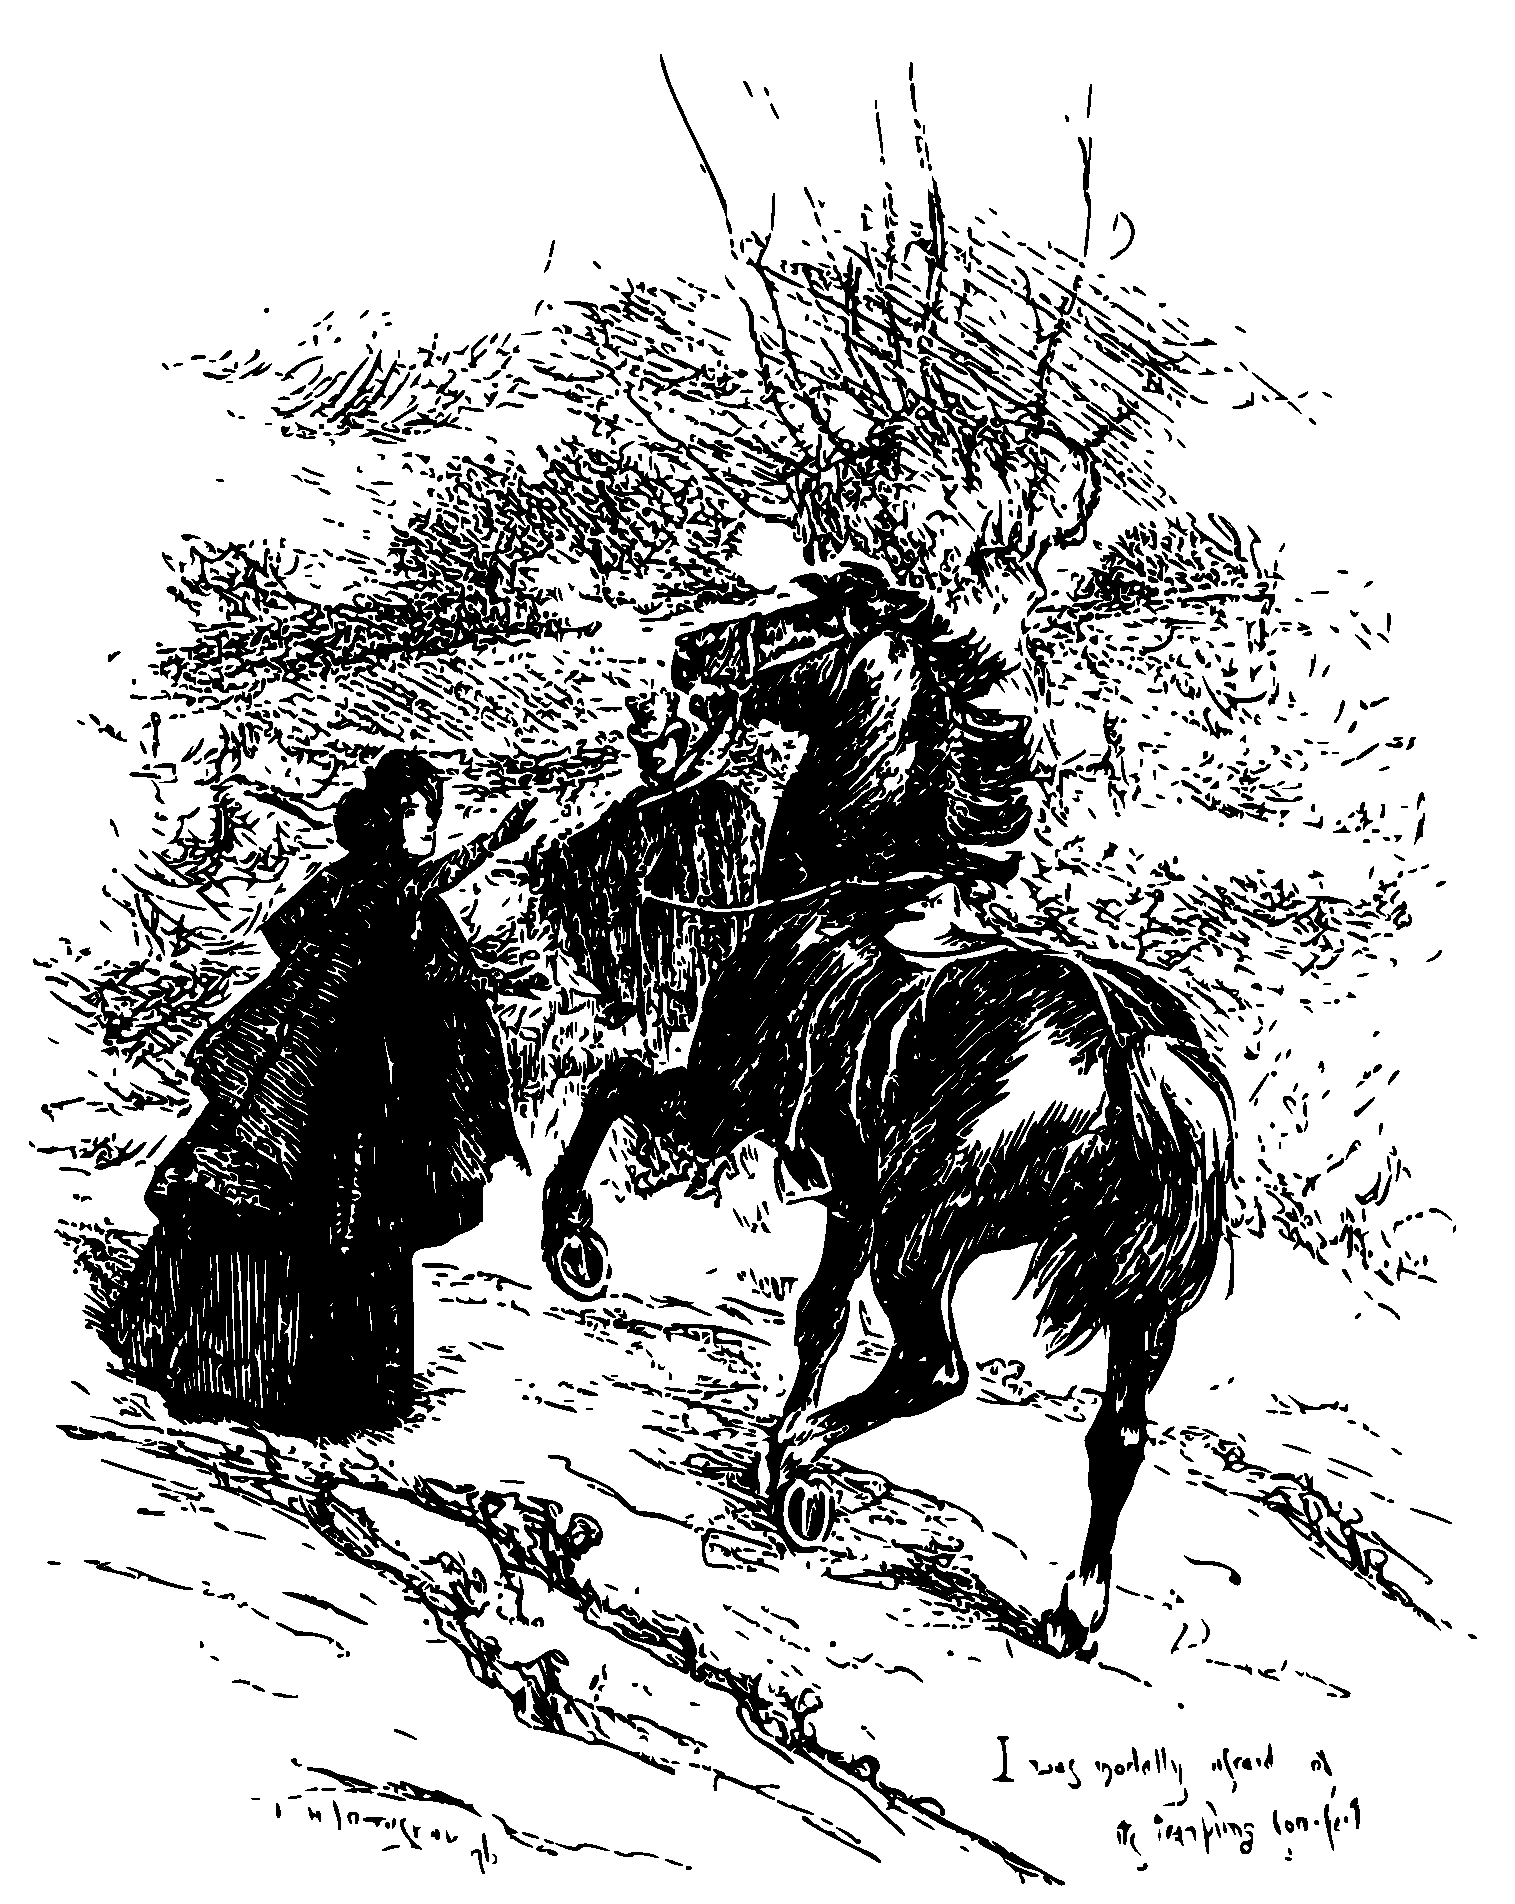
\includegraphics[width=\linewidth]{images/p107b.pdf}
	\end{sidecaption}
\end{figure}

\enquote{I see,} he said, \enquote{the mountain will never be brought to
Mahomet, so all you can do is to aid Mahomet to go to the mountain; I
must beg of you to come here.}

I came. \enquote{Excuse me,} he continued: \enquote{necessity compels
me to make you useful.} He laid a heavy hand on my shoulder, and
leaning on me with some stress, limped to his horse. Having once caught
the bridle, he mastered it directly and sprang to his saddle; grimacing
grimly as he made the effort, for it wrenched his sprain.

\enquote{Now,} said he, releasing his under lip from a hard bite,
\enquote{just hand me my whip; it lies there under the hedge.}

I sought it and found it.

\enquote{Thank you; now make haste with the letter to Hay, and return as
fast as you can.}

A touch of a spurred heel made his horse first start and rear, and then
bound away; the dog rushed in his traces; all three vanished,

\settoversewidth{\versewidth}{'Like heath that, in the wilderness,}
\begin{verse}[\versewidth]
\enquote{Like heath that, in the wilderness,\\*
The wild wind whirls away.}
\end{verse}

I took up my muff and walked on. The incident had occurred and was gone
for me: it \emph{was} an incident of no moment, no romance, no interest
in a sense; yet it marked with change one single hour of a monotonous
life. My help had been needed and claimed; I had given it: I was
pleased to have done something; trivial, transitory though the deed was,
it was yet an active thing, and I was weary of an existence all
passive. The new face, too, was like a new picture introduced to the
gallery of memory; and it was dissimilar to all the others hanging
there: firstly, because it was masculine; and, secondly, because it was
dark, strong, and stern. I had it still before me when I entered Hay,
and slipped the letter into the post-office; I saw it as I walked fast
down-hill all the way home. When I came to the stile, I stopped a
minute, looked round and listened, with an idea that a horse's hoofs
might ring on the causeway again, and that a rider in a cloak, and a
Gytrash-like Newfoundland dog, might be again apparent: I saw only the
hedge and a pollard willow before me, rising up still and straight to
meet the moonbeams; I heard only the faintest waft of wind roaming
fitful among the trees round Thornfield, a mile distant; and when I
glanced down in the direction of the murmur, my eye, traversing the
hall-front, caught a light kindling in a window: it reminded me that I
was late, and I hurried on.

I did not like re-entering Thornfield. To pass its threshold was to
return to stagnation; to cross the silent hall, to ascend the darksome
staircase, to seek my own lonely little room, and then to meet tranquil
\Mrs{} Fairfax, and spend the long winter evening with her, and her only,
was to quell wholly the faint excitement wakened by my walk,---to slip
again over my faculties the viewless fetters of an uniform and too still
existence; of an existence whose very privileges of security and ease I
was becoming incapable of appreciating. What good it would have done me
at that time to have been tossed in the storms of an uncertain
struggling life, and to have been taught by rough and bitter experience
to long for the calm amidst which I now repined! Yes, just as much good
as it would do a man tired of sitting still in a \enquote{too easy
chair} to take a long walk: and just as natural was the wish to stir,
under my circumstances, as it would be under his.

I lingered at the gates; I lingered on the lawn; I paced backwards and
forwards on the pavement; the shutters of the glass door were closed; I
could not see into the interior; and both my eyes and spirit seemed
drawn from the gloomy house---from the grey-hollow filled with rayless
cells, as it appeared to me---to that sky expanded before me,---a blue
sea absolved from taint of cloud; the moon ascending it in solemn march;
her orb seeming to look up as she left the hill-tops, from behind which
she had come, far and farther below her, and aspired to the zenith,
midnight dark in its fathomless depth and measureless distance; and for
those trembling stars that followed her course; they made my heart
tremble, my veins glow when I viewed them. Little things recall us to
earth; the clock struck in the hall; that sufficed; I turned from moon
and stars, opened a side-door, and went in.

The hall was not dark, nor yet was it lit, only by the high-hung bronze
lamp; a warm glow suffused both it and the lower steps of the oak
staircase. This ruddy shine issued from the great dining-room, whose
two-leaved door stood open, and showed a genial fire in the grate,
glancing on marble hearth and brass fire-irons, and revealing purple
draperies and polished furniture, in the most pleasant radiance. It
revealed, too, a group near the mantelpiece: I had scarcely caught it,
and scarcely become aware of a cheerful mingling of voices, amongst
which I seemed to distinguish the tones of Adèle, when the door closed.

I hastened to \Mrs{} Fairfax's room; there was a fire there too, but no
candle, and no \Mrs{} Fairfax. Instead, all alone, sitting upright on the
rug, and gazing with gravity at the blaze, I beheld a great black and
white long-haired dog, just like the Gytrash of the lane. It was so
like it that I went forward and said---\enquote{Pilot} and the thing got
up and came to me and snuffed me. I caressed him, and he wagged his
great tail; but he looked an eerie creature to be alone with, and I
could not tell whence he had come. I rang the bell, for I wanted a
candle; and I wanted, too, to get an account of this visitant. Leah
entered.

\enquote{What dog is this?}

\enquote{He came with master.}

\enquote{With whom?}

\enquote{With master---\Mr{} Rochester---he is just arrived.}

\enquote{Indeed! and is \Mrs{} Fairfax with him?}

\enquote{Yes, and Miss Adèle; they are in the dining-room, and John is
gone for a surgeon; for master has had an accident; his horse fell and
his ankle is sprained.}

\enquote{Did the horse fall in Hay Lane?}

\enquote{Yes, coming down-hill; it slipped on some ice.}

\enquote{Ah! Bring me a candle will you Leah?}

Leah brought it; she entered, followed by \Mrs{} Fairfax, who repeated the
news; adding that \Mr{} Carter the surgeon was come, and was now with \Mr{}
 Rochester: then she hurried out to give orders about tea, and I went
upstairs to take off my things.

\FChapter{Chapter Thirteen}{13}

\Lettrine{M}{r.\@} \textsc{ Rochester,} it seems, by the surgeon's orders, went to bed early that
night; nor did he rise soon next morning. When he did come down, it was
to attend to business: his agent and some of his tenants were arrived,
and waiting to speak with him.

Adèle and I had now to vacate the library: it would be in daily
requisition as a reception-room for callers. A fire was lit in an
apartment upstairs, and there I carried our books, and arranged it for
the future schoolroom. I discerned in the course of the morning that
Thornfield Hall was a changed place: no longer silent as a church, it
echoed every hour or two to a knock at the door, or a clang of the bell;
steps, too, often traversed the hall, and new voices spoke in different
keys below; a rill from the outer world was flowing through it; it had a
master: for my part, I liked it better.

Adèle was not easy to teach that day; she could not apply: she kept
running to the door and looking over the banisters to see if she could
get a glimpse of \Mr{} Rochester; then she coined pretexts to go
downstairs, in order, as I shrewdly suspected, to visit the library,
where I knew she was not wanted; then, when I got a little angry, and
made her sit still, she continued to talk incessantly of her \foreignquote{french}{ami,
Monsieur Edouard Fairfax \emph{de} Rochester,} as she dubbed him (I had
not before heard his prenomens), and to conjecture what presents he had
brought her: for it appears he had intimated the night before, that when
his luggage came from Millcote, there would be found amongst it a little
box in whose contents she had an interest.

\foreignquote{french}{Et cela doit signifier,} said she, \foreignquote{french}{qu'il y aura là
dedans un cadeau pour moi, et peut-être pour vous aussi, mademoiselle. 
Monsieur a parlé de vous: il m'a demandé le nom de ma gouvernante, et si
elle n'était pas une petite personne, assez mince et un peu pâle. J'ai
dit qu'oui: car c'est vrai, n'est-ce pas, mademoiselle?}\footnote{%
\enquote{And that must mean,} \textelp{} \enquote{that there will be a present
for me in there, and perhaps for you too, miss. \Mr{} has talked about you:
he asked me the name of my governess, and whether she wasn't a small
person, quite thin and rather pale. I said yes: for it's true, isn't it, miss?}}

I and my pupil dined as usual in \Mrs{} Fairfax's parlour; the afternoon
was wild and snowy, and we passed it in the schoolroom. At dark I
allowed Adèle to put away books and work, and to run downstairs; for,
from the comparative silence below, and from the cessation of appeals to
the door-bell, I conjectured that \Mr{} Rochester was now at liberty. 
Left alone, I walked to the window; but nothing was to be seen thence:
twilight and snowflakes together thickened the air, and hid the very
shrubs on the lawn. I let down the curtain and went back to the
fireside.

In the clear embers I was tracing a view, not unlike a picture I
remembered to have seen of the castle of Heidelberg, on the Rhine, when
\Mrs{} Fairfax came in, breaking up by her entrance the fiery mosaic I had
been piercing together, and scattering too some heavy unwelcome thoughts
that were beginning to throng on my solitude.

\enquote{\Mr{} Rochester would be glad if you and your pupil would take
tea with him in the drawing-room this evening,} said she: \enquote{he
has been so much engaged all day that he could not ask to see you
before.}

\enquote{When is his tea-time?} I inquired.

\enquote{Oh, at six o'clock: he keeps early hours in the country. You
had better change your frock now; I will go with you and fasten it. 
Here is a candle.}

\enquote{Is it necessary to change my frock?}

\enquote{Yes, you had better: I always dress for the evening when \Mr{}
 Rochester is here.}

This additional ceremony seemed somewhat stately; however, I repaired to
my room, and, with \Mrs{} Fairfax's aid, replaced my black stuff dress by
one of black silk; the best and the only additional one I had, except
one of light grey, which, in my Lowood notions of the toilette, I
thought too fine to be worn, except on first-rate occasions.

\enquote{You want a brooch,} said \Mrs{} Fairfax. I had a single little
pearl ornament which Miss Temple gave me as a parting keepsake: I put it
on, and then we went downstairs. Unused as I was to strangers, it was
rather a trial to appear thus formally summoned in \Mr{} Rochester's
presence. I let \Mrs{} Fairfax precede me into the dining-room, and kept
in her shade as we crossed that apartment; and, passing the arch, whose
curtain was now dropped, entered the elegant recess beyond.

Two wax candles stood lighted on the table, and two on the mantelpiece;
basking in the light and heat of a superb fire, lay Pilot---Adèle knelt
near him. Half reclined on a couch appeared \Mr{} Rochester, his foot
supported by the cushion; he was looking at Adèle and the dog: the fire
shone full on his face. I knew my traveller with his broad and jetty
eyebrows; his square forehead, made squarer by the horizontal sweep of
his black hair. I recognised his decisive nose, more remarkable for
character than beauty; his full nostrils, denoting, I thought, choler;
his grim mouth, chin, and jaw---yes, all three were very grim, and no
mistake. His shape, now divested of cloak, I perceived harmonised in
squareness with his physiognomy: I suppose it was a good figure in the
athletic sense of the term---broad chested and thin flanked, though
neither tall nor graceful.

\Mr{} Rochester must have been aware of the entrance of \Mrs{} Fairfax and
myself; but it appeared he was not in the mood to notice us, for he
never lifted his head as we approached.

\enquote{Here is Miss Eyre, sir,} said \Mrs{} Fairfax, in her quiet way. 
He bowed, still not taking his eyes from the group of the dog and child.

\enquote{Let Miss Eyre be seated,} said he: and there was something in
the forced stiff bow, in the impatient yet formal tone, which seemed
further to express, \enquote{What the deuce is it to me whether Miss
Eyre be there or not? At this moment I am not disposed to accost her.}

I sat down quite disembarrassed. A reception of finished politeness
would probably have confused me: I could not have returned or repaid it
by answering grace and elegance on my part; but harsh caprice laid me
under no obligation; on the contrary, a decent quiescence, under the
freak of manner, gave me the advantage. Besides, the eccentricity of
the proceeding was piquant: I felt interested to see how he would go on.

He went on as a statue would, that is, he neither spoke nor moved. \Mrs{}
Fairfax seemed to think it necessary that some one should be amiable,
and she began to talk. Kindly, as usual---and, as usual, rather
trite---she condoled with him on the pressure of business he had had all
day; on the annoyance it must have been to him with that painful sprain:
then she commended his patience and perseverance in going through with
it.

\enquote{Madam, I should like some tea,} was the sole rejoinder she
got. She hastened to ring the bell; and when the tray came, she
proceeded to arrange the cups, spoons, \etc, with assiduous celerity. I
and Adèle went to the table; but the master did not leave his couch.

\enquote{Will you hand \Mr{} Rochester's cup?} said \Mrs{} Fairfax to me;
\enquote{Adèle might perhaps spill it.}

I did as requested. As he took the cup from my hand, Adèle, thinking
the moment propitious for making a request in my favour, cried out---

\foreignquote{french}{N'est-ce pas, monsieur, qu'il y a un cadeau pour Mademoiselle
Eyre dans votre petit coffre?}\footnote{\enquote{There's a present for Miss, isn't there, sir, in your little chest?}}

\enquote{Who talks of \foreignlanguage{french}{cadeaux}?} said he gruffly. \enquote{Did you
expect a present, Miss Eyre? Are you fond of presents?} and he searched
my face with eyes that I saw were dark, irate, and piercing.

\enquote{I hardly know, sir; I have little experience of them: they are
generally thought pleasant things.}

\enquote{Generally thought? But what do \emph{you} think?}

\enquote{I should be obliged to take time, sir, before I could give you
an answer worthy of your acceptance: a present has many faces to it, has
it not? and one should consider all, before pronouncing an opinion as to
its nature.}

\enquote{Miss Eyre, you are not so unsophisticated as Adèle: she demands
a \foreignquote{french}{cadeau,} clamorously, the moment she sees me: you beat about
the bush.}

\enquote{Because I have less confidence in my deserts than Adèle has:
she can prefer the claim of old acquaintance, and the right too of
custom; for she says you have always been in the habit of giving her
playthings; but if I had to make out a case I should be puzzled, since I
am a stranger, and have done nothing to entitle me to an
acknowledgment.}

\enquote{Oh, don't fall back on over-modesty! I have examined Adèle,
and find you have taken great pains with her: she is not bright, she has
no talents; yet in a short time she has made much improvement.}

\enquote{Sir, you have now given me my \foreignquote{french}{cadeau}; I am obliged
to you: it is the meed teachers most covet---praise of their pupils'
progress.}

\enquote{Humph!} said \Mr{} Rochester, and he took his tea in silence.

\enquote{Come to the fire,} said the master, when the tray was taken
away, and \Mrs{} Fairfax had settled into a corner with her knitting;
while Adèle was leading me by the hand round the room, showing me the
beautiful books and ornaments on the consoles and chiffonnières. We
obeyed, as in duty bound; Adèle wanted to take a seat on my knee, but
she was ordered to amuse herself with Pilot.

\enquote{You have been resident in my house three months?}

\enquote{Yes, sir.}

\enquote{And you came from---?}

\enquote{From Lowood school, in ---shire.}

\enquote{Ah! a charitable concern. How long were you there?}

\enquote{Eight years.}

\enquote{Eight years! you must be tenacious of life. I thought half the
time in such a place would have done up any constitution! No wonder you
have rather the look of another world. I marvelled where you had got
that sort of face. When you came on me in Hay Lane last night, I
thought unaccountably of fairy tales, and had half a mind to demand
whether you had bewitched my horse: I am not sure yet. Who are your
parents?}

\enquote{I have none.}

\enquote{Nor ever had, I suppose: do you remember them?}

\enquote{No.}

\enquote{I thought not. And so you were waiting for your people when
you sat on that stile?}

\enquote{For whom, sir?}

\enquote{For the men in green: it was a proper moonlight evening for
them. Did I break through one of your rings, that you spread that
damned ice on the causeway?}

I shook my head. \enquote{The men in green all forsook England a
hundred years ago,} said I, speaking as seriously as he had done. 
\enquote{And not even in Hay Lane, or the fields about it, could you
find a trace of them. I don't think either summer or harvest, or winter
moon, will ever shine on their revels more.}

\Mrs{} Fairfax had dropped her knitting, and, with raised eyebrows, seemed
wondering what sort of talk this was.

\enquote{Well,} resumed \Mr{} Rochester, \enquote{if you disown parents,
you must have some sort of kinsfolk: uncles and aunts?}

\enquote{No; none that I ever saw.}

\enquote{And your home?}

\enquote{I have none.}

\enquote{Where do your brothers and sisters live?}

\enquote{I have no brothers or sisters.}

\enquote{Who recommended you to come here?}

\enquote{I advertised, and \Mrs{} Fairfax answered my advertisement.}

\enquote{Yes,} said the good lady, who now knew what ground we were
upon, \enquote{and I am daily thankful for the choice Providence led me
to make. Miss Eyre has been an invaluable companion to me, and a kind
and careful teacher to Adèle.}

\enquote{Don't trouble yourself to give her a character,} returned \Mr{}
 Rochester: \enquote{eulogiums will not bias me; I shall judge for
myself. She began by felling my horse.}

\enquote{Sir?} said \Mrs{} Fairfax.

\enquote{I have to thank her for this sprain.}

The widow looked bewildered.

\enquote{Miss Eyre, have you ever lived in a town?}

\enquote{No, sir.}

\enquote{Have you seen much society?}

\enquote{None but the pupils and teachers of Lowood, and now the inmates
of Thornfield.}

\enquote{Have you read much?}

\enquote{Only such books as came in my way; and they have not been
numerous or very learned.}

\enquote{You have lived the life of a nun: no doubt you are well drilled
in religious forms;---Brocklehurst, who I understand directs Lowood, is
a parson, is he not?}

\enquote{Yes, sir.}

\enquote{And you girls probably worshipped him, as a convent full of
religieuses would worship their director.}

\enquote{Oh, no.}

\enquote{You are very cool! No! What! a novice not worship her
priest! That sounds blasphemous.}

\enquote{I disliked \Mr{} Brocklehurst; and I was not alone in the
feeling. He is a harsh man; at once pompous and meddling; he cut off
our hair; and for economy's sake bought us bad needles and thread, with
which we could hardly sew.}

\enquote{That was very false economy,} remarked \Mrs{} Fairfax, who now
again caught the drift of the dialogue.

\enquote{And was that the head and front of his offending?} demanded \Mr{}
 Rochester.

\enquote{He starved us when he had the sole superintendence of the
provision department, before the committee was appointed; and he bored
us with long lectures once a week, and with evening readings from books
of his own inditing, about sudden deaths and judgments, which made us
afraid to go to bed.}

\enquote{What age were you when you went to Lowood?}

\enquote{About ten.}

\enquote{And you stayed there eight years: you are now, then, eighteen?}

I assented.

\enquote{Arithmetic, you see, is useful; without its aid, I should
hardly have been able to guess your age. It is a point difficult to fix
where the features and countenance are so much at variance as in your
case. And now what did you learn at Lowood? Can you play?}

\enquote{A little.}

\enquote{Of course: that is the established answer. Go into the
library---I mean, if you please.---(Excuse my tone of command; I am used
to say, \enquote{Do this,} and it is done: I cannot alter my customary
habits for one new inmate.)---Go, then, into the library; take a candle
with you; leave the door open; sit down to the piano, and play a tune.}

I departed, obeying his directions.

\enquote{Enough!} he called out in a few minutes. \enquote{You play \emph{a
little}, I see; like any other English school-girl; perhaps rather
better than some, but not well.}

I closed the piano and returned. \Mr{} Rochester
continued---\enquote{Adèle showed me some sketches this morning, which
she said were yours. I don't know whether they were entirely of your
doing; probably a master aided you?}

\enquote{No, indeed!} I interjected.

\enquote{Ah! that pricks pride. Well, fetch me your portfolio, if you
can vouch for its contents being original; but don't pass your word
unless you are certain: I can recognise patchwork.}

\enquote{Then I will say nothing, and you shall judge for yourself,
sir.}

I brought the portfolio from the library.

\enquote{Approach the table,} said he; and I wheeled it to his couch. 
Adèle and \Mrs{} Fairfax drew near to see the pictures.

\enquote{No crowding,} said \Mr{} Rochester: \enquote{take the drawings
from my hand as I finish with them; but don't push your faces up to
mine.}

He deliberately scrutinised each sketch and painting. Three he laid
aside; the others, when he had examined them, he swept from him.

\enquote{Take them off to the other table, \Mrs{} Fairfax,} said he,
\enquote{and look at them with Adèle;---you} (glancing at me)
\enquote{resume your seat, and answer my questions. I perceive those
pictures were done by one hand: was that hand yours?}

\enquote{Yes.}

\enquote{And when did you find time to do them? They have taken much
time, and some thought.}

\enquote{I did them in the last two vacations I spent at Lowood, when I
had no other occupation.}

\enquote{Where did you get your copies?}

\enquote{Out of my head.}

\enquote{That head I see now on your shoulders?}

\enquote{Yes, sir.}

\enquote{Has it other furniture of the same kind within?}

\enquote{I should think it may have: I should hope---better.}

He spread the pictures before him, and again surveyed them alternately.

While he is so occupied, I will tell you, reader, what they are: and
first, I must premise that they are nothing wonderful. The subjects
had, indeed, risen vividly on my mind. As I saw them with the spiritual
eye, before I attempted to embody them, they were striking; but my hand
would not second my fancy, and in each case it had wrought out but a
pale portrait of the thing I had conceived.

These pictures were in water-colours. The first represented clouds low
and livid, rolling over a swollen sea: all the distance was in eclipse;
so, too, was the foreground; or rather, the nearest billows, for there
was no land. One gleam of light lifted into relief a half-submerged
mast, on which sat a cormorant, dark and large, with wings flecked with
foam; its beak held a gold bracelet set with gems, that I had touched
with as brilliant tints as my palette could yield, and as glittering
distinctness as my pencil could impart. Sinking below the bird and
mast, a drowned corpse glanced through the green water; a fair arm was
the only limb clearly visible, whence the bracelet had been washed or
torn.

The second picture contained for foreground only the dim peak of a hill,
with grass and some leaves slanting as if by a breeze. Beyond and above
spread an expanse of sky, dark blue as at twilight: rising into the sky
was a woman's shape to the bust, portrayed in tints as dusk and soft as
I could combine. The dim forehead was crowned with a star; the
lineaments below were seen as through the suffusion of vapour; the eyes
shone dark and wild; the hair streamed shadowy, like a beamless cloud
torn by storm or by electric travail. On the neck lay a pale reflection
like moonlight; the same faint lustre touched the train of thin clouds
from which rose and bowed this vision of the Evening Star.

The third showed the pinnacle of an iceberg piercing a polar winter sky:
a muster of northern lights reared their dim lances, close serried,
along the horizon. Throwing these into distance, rose, in the
foreground, a head,---a colossal head, inclined towards the iceberg, and
resting against it. Two thin hands, joined under the forehead, and
supporting it, drew up before the lower features a sable veil, a brow
quite bloodless, white as bone, and an eye hollow and fixed, blank of
meaning but for the glassiness of despair, alone were visible. Above
the temples, amidst wreathed turban folds of black drapery, vague in its
character and consistency as cloud, gleamed a ring of white flame,
gemmed with sparkles of a more lurid tinge. This pale crescent was
\enquote{the likeness of a kingly crown;} what it diademed was
\enquote{the shape which shape had none.}

\enquote{Were you happy when you painted these pictures?} asked \Mr{}
 Rochester presently.

\enquote{I was absorbed, sir: yes, and I was happy. To paint them, in
short, was to enjoy one of the keenest pleasures I have ever known.}

\enquote{That is not saying much. Your pleasures, by your own account,
have been few; but I daresay you did exist in a kind of artist's
dreamland while you blent and arranged these strange tints. Did you sit
at them long each day?}

\enquote{I had nothing else to do, because it was the vacation, and I
sat at them from morning till noon, and from noon till night: the length
of the midsummer days favoured my inclination to apply.}

\enquote{And you felt self-satisfied with the result of your ardent
labours?}

\enquote{Far from it. I was tormented by the contrast between my idea
and my handiwork: in each case I had imagined something which I was
quite powerless to realise.}

\enquote{Not quite: you have secured the shadow of your thought; but no
more, probably. You had not enough of the artist's skill and science to
give it full being: yet the drawings are, for a school-girl, peculiar. 
As to the thoughts, they are elfish. These eyes in the Evening Star you
must have seen in a dream. How could you make them look so clear, and
yet not at all brilliant? for the planet above quells their rays. And
what meaning is that in their solemn depth? And who taught you to paint
wind? There is a high gale in that sky, and on this hill-top. Where
did you see Latmos? For that is Latmos. There! put the drawings away!}

I had scarce tied the strings of the portfolio, when, looking at his
watch, he said abruptly---

\enquote{It is nine o'clock: what are you about, Miss Eyre, to let Adèle
sit up so long? Take her to bed.}

Adèle went to kiss him before quitting the room: he endured the caress,
but scarcely seemed to relish it more than Pilot would have done, nor so
much.

\enquote{I wish you all good-night, now,} said he, making a movement of
the hand towards the door, in token that he was tired of our company,
and wished to dismiss us. \Mrs{} Fairfax folded up her knitting: I took
my portfolio: we curtseyed to him, received a frigid bow in return, and
so withdrew.

\enquote{You said \Mr{} Rochester was not strikingly peculiar, \Mrs{}
Fairfax,} I observed, when I rejoined her in her room, after putting
Adèle to bed.

\enquote{Well, is he?}

\enquote{I think so: he is very changeful and abrupt.}

\enquote{True: no doubt he may appear so to a stranger, but I am so
accustomed to his manner, I never think of it; and then, if he has
peculiarities of temper, allowance should be made.}

\enquote{Why?}

\enquote{Partly because it is his nature---and we can none of us help
our nature; and partly because he has painful thoughts, no doubt, to
harass him, and make his spirits unequal.}

\enquote{What about?}

\enquote{Family troubles, for one thing.}

\enquote{But he has no family.}

\enquote{Not now, but he has had---or, at least, relatives. He lost his
elder brother a few years since.}

\enquote{His \emph{elder} brother?}

\enquote{Yes. The present \Mr{} Rochester has not been very long in
possession of the property; only about nine years.}

\enquote{Nine years is a tolerable time. Was he so very fond of his
brother as to be still inconsolable for his loss?}

\enquote{Why, no---perhaps not. I believe there were some
misunderstandings between them. \Mr{} Rowland Rochester was not quite
just to \Mr{} Edward; and perhaps he prejudiced his father against him. 
The old gentleman was fond of money, and anxious to keep the family
estate together. He did not like to diminish the property by division,
and yet he was anxious that \Mr{} Edward should have wealth, too, to keep
up the consequence of the name; and, soon after he was of age, some
steps were taken that were not quite fair, and made a great deal of
mischief. Old \Mr{} Rochester and \Mr{} Rowland combined to bring \Mr{}
Edward into what he considered a painful position, for the sake of
making his fortune: what the precise nature of that position was I never
clearly knew, but his spirit could not brook what he had to suffer in
it. He is not very forgiving: he broke with his family, and now for
many years he has led an unsettled kind of life. I don't think he has
ever been resident at Thornfield for a fortnight together, since the
death of his brother without a will left him master of the estate; and,
indeed, no wonder he shuns the old place.}

\enquote{Why should he shun it?}

\enquote{Perhaps he thinks it gloomy.}

The answer was evasive. I should have liked something clearer; but \Mrs{}
Fairfax either could not, or would not, give me more explicit
information of the origin and nature of \Mr{} Rochester's trials. She
averred they were a mystery to herself, and that what she knew was
chiefly from conjecture. It was evident, indeed, that she wished me to
drop the subject, which I did accordingly.

\FChapter{Chapter Fourteen}{14}

\Lettrine{F}{or} \textsc{several subsequent days} I saw little of \Mr{} Rochester. In the
mornings he seemed much engaged with business, and, in the afternoon,
gentlemen from Millcote or the neighbourhood called, and sometimes
stayed to dine with him. When his sprain was well enough to admit of
horse exercise, he rode out a good deal; probably to return these
visits, as he generally did not come back till late at night.

During this interval, even Adèle was seldom sent for to his presence,
and all my acquaintance with him was confined to an occasional rencontre
in the hall, on the stairs, or in the gallery, when he would sometimes
pass me haughtily and coldly, just acknowledging my presence by a
distant nod or a cool glance, and sometimes bow and smile with
gentlemanlike affability. His changes of mood did not offend me,
because I saw that I had nothing to do with their alternation; the ebb
and flow depended on causes quite disconnected with me.

One day he had had company to dinner, and had sent for my portfolio; in
order, doubtless, to exhibit its contents: the gentlemen went away
early, to attend a public meeting at Millcote, as \Mrs{} Fairfax informed
me; but the night being wet and inclement, \Mr{} Rochester did not
accompany them. Soon after they were gone he rang the bell: a message
came that I and Adèle were to go downstairs. I brushed Adèle's hair and
made her neat, and having ascertained that I was myself in my usual
Quaker trim, where there was nothing to retouch---all being too close
and plain, braided locks included, to admit of disarrangement---we
descended, Adèle wondering whether the \foreignlanguage{french}{\emph{petit coffre}} was at length
come; for, owing to some mistake, its arrival had hitherto been
delayed. She was gratified: there it stood, a little carton, on the
table when we entered the dining-room. She appeared to know it by
instinct.

\foreignquote{french}{Ma boite! ma boite!}\footnote{\enquote{My box! my box!}} exclaimed she, running towards it.

\enquote{Yes, there is your \foreignquote{french}{boite} at last: take it into a
corner, you genuine daughter of Paris, and amuse yourself with
disembowelling it,} said the deep and rather sarcastic voice of \Mr{}
 Rochester, proceeding from the depths of an immense easy-chair at the
fireside. \enquote{And mind,} he continued, \enquote{don't bother me
with any details of the anatomical process, or any notice of the
condition of the entrails: let your operation be conducted in silence:
\foreignlanguage{french}{tiens-toi tranquille, enfant; comprends-tu?}\footnote{\enquote{Keep quiet, child; do you understand?}}}

Adèle seemed scarcely to need the warning---she had already retired to a
sofa with her treasure, and was busy untying the cord which secured the
lid. Having removed this impediment, and lifted certain silvery
envelopes of tissue paper, she merely exclaimed---

\foreignquote{french}{Oh ciel! Que c'est beau!}\footnote{\enquote{Oh heavens! How lovely!}} and then remained absorbed in
ecstatic contemplation.

\enquote{Is Miss Eyre there?} now demanded the master, half rising from
his seat to look round to the door, near which I still stood.

\enquote{Ah! well, come forward; be seated here.} He drew a chair near
his own. \enquote{I am not fond of the prattle of children,} he
continued; \enquote{for, old bachelor as I am, I have no pleasant associations
connected with their lisp. It would be intolerable to me to pass a
whole evening \emph{tête-à-tête} with a brat. Don't draw that chair
farther off, Miss Eyre; sit down exactly where I placed it---if you
please, that is. Confound these civilities! I continually forget
them. Nor do I particularly affect simple-minded old ladies. 
By-the-bye, I must have mine in mind; it won't do to neglect her; she is
a Fairfax, or wed to one; and blood is said to be thicker than water.}

He rang, and despatched an invitation to \Mrs{} Fairfax, who soon arrived,
knitting-basket in hand.

\enquote{Good evening, madam; I sent to you for a charitable purpose. I
have forbidden Adèle to talk to me about her presents, and she is
bursting with repletion: have the goodness to serve her as auditress and
interlocutrice; it will be one of the most benevolent acts you ever
performed.}

Adèle, indeed, no sooner saw \Mrs{} Fairfax, than she summoned her to her
sofa, and there quickly filled her lap with the porcelain, the ivory,
the waxen contents of her \foreignquote{french}{boite;} pouring out, meantime,
explanations and raptures in such broken English as she was mistress of.

\enquote{Now I have performed the part of a good host,} pursued \Mr{}
 Rochester, \enquote{put my guests into the way of amusing each other, I
ought to be at liberty to attend to my own pleasure. Miss Eyre, draw
your chair still a little farther forward: you are yet too far back; I
cannot see you without disturbing my position in this comfortable chair,
which I have no mind to do.}

I did as I was bid, though I would much rather have remained somewhat in
the shade; but \Mr{} Rochester had such a direct way of giving orders, it
seemed a matter of course to obey him promptly.

We were, as I have said, in the dining-room: the lustre, which had been
lit for dinner, filled the room with a festal breadth of light; the
large fire was all red and clear; the purple curtains hung rich and
ample before the lofty window and loftier arch; everything was still,
save the subdued chat of Adèle (she dared not speak loud), and, filling
up each pause, the beating of winter rain against the panes.

\Mr{} Rochester, as he sat in his damask-covered chair, looked different
to what I had seen him look before; not quite so stern---much less
gloomy. There was a smile on his lips, and his eyes sparkled, whether
with wine or not, I am not sure; but I think it very probable. He was,
in short, in his after-dinner mood; more expanded and genial, and also
more self-indulgent than the frigid and rigid temper of the morning;
still he looked preciously grim, cushioning his massive head against the
swelling back of his chair, and receiving the light of the fire on his
granite-hewn features, and in his great, dark eyes; for he had great,
dark eyes, and very fine eyes, too---not without a certain change in
their depths sometimes, which, if it was not softness, reminded you, at
least, of that feeling.

He had been looking two minutes at the fire, and I had been looking the
same length of time at him, when, turning suddenly, he caught my gaze
fastened on his physiognomy.

\enquote{You examine me, Miss Eyre,} said he: \enquote{do you think me
handsome?}

I should, if I had deliberated, have replied to this question by
something conventionally vague and polite; but the answer somehow
slipped from my tongue before I was aware---\enquote{No, sir.}

\enquote{Ah! By my word! there is something singular about you,} said
he: \enquote{you have the air of a little \emph{nonnette}; quaint, quiet,
grave, and simple, as you sit with your hands before you, and your eyes
generally bent on the carpet (except, by-the-bye, when they are directed
piercingly to my face; as just now, for instance); and when one asks you
a question, or makes a remark to which you are obliged to reply, you rap
out a round rejoinder, which, if not blunt, is at least brusque. What
do you mean by it?}

\enquote{Sir, I was too plain; I beg your pardon. I ought to have
replied that it was not easy to give an impromptu answer to a question
about appearances; that tastes mostly differ; and that beauty is of
little consequence, or something of that sort.}

\enquote{You ought to have replied no such thing. Beauty of little
consequence, indeed! And so, under pretence of softening the previous
outrage, of stroking and soothing me into placidity, you stick a sly
penknife under my ear! Go on: what fault do you find with me, pray? I
suppose I have all my limbs and all my features like any other man?}

\enquote{\Mr{} Rochester, allow me to disown my first answer: I intended
no pointed repartee: it was only a blunder.}

\enquote{Just so: I think so: and you shall be answerable for it. 
Criticise me: does my forehead not please you?}

He lifted up the sable waves of hair which lay horizontally over his
brow, and showed a solid enough mass of intellectual organs, but an
abrupt deficiency where the suave sign of benevolence should have risen.

\enquote{Now, ma'am, am I a fool?}

\enquote{Far from it, sir. You would, perhaps, think me rude if I
inquired in return whether you are a philanthropist?}

\enquote{There again! Another stick of the penknife, when she pretended
to pat my head: and that is because I said I did not like the society of
children and old women (low be it spoken!). No, young lady, I am not a
general philanthropist; but I bear a conscience;} and he pointed to the
prominences which are said to indicate that faculty, and which,
fortunately for him, were sufficiently conspicuous; giving, indeed, a
marked breadth to the upper part of his head: \enquote{and, besides, I
once had a kind of rude tenderness of heart. When I was as old as you,
I was a feeling fellow enough, partial to the unfledged, unfostered, and
unlucky; but Fortune has knocked me about since: she has even kneaded me
with her knuckles, and now I flatter myself I am hard and tough as an
India-rubber ball; pervious, though, through a chink or two still, and
with one sentient point in the middle of the lump. Yes: does that leave
hope for me?}

\enquote{Hope of what, sir?}

\enquote{Of my final re-transformation from India-rubber back to flesh?}

\enquote{Decidedly he has had too much wine,} I thought; and I did not
know what answer to make to his queer question: how could I tell whether
he was capable of being re-transformed?

\enquote{You looked very much puzzled, Miss Eyre; and though you are not
pretty any more than I am handsome, yet a puzzled air becomes you;
besides, it is convenient, for it keeps those searching eyes of yours
away from my physiognomy, and busies them with the worsted flowers of
the rug; so puzzle on. Young lady, I am disposed to be gregarious and
communicative to-night.}

With this announcement he rose from his chair, and stood, leaning his
arm on the marble mantelpiece: in that attitude his shape was seen
plainly as well as his face; his unusual breadth of chest,
disproportionate almost to his length of limb. I am sure most people
would have thought him an ugly man; yet there was so much unconscious
pride in his port; so much ease in his demeanour; such a look of
complete indifference to his own external appearance; so haughty a
reliance on the power of other qualities, intrinsic or adventitious, to
atone for the lack of mere personal attractiveness, that, in looking at
him, one inevitably shared the indifference, and, even in a blind,
imperfect sense, put faith in the confidence.

\enquote{I am disposed to be gregarious and communicative to-night,} he
repeated, \enquote{and that is why I sent for you: the fire and the
chandelier were not sufficient company for me; nor would Pilot have
been, for none of these can talk. Adèle is a degree better, but still
far below the mark; \Mrs{} Fairfax ditto; you, I am persuaded, can suit me
if you will: you puzzled me the first evening I invited you down here. 
I have almost forgotten you since: other ideas have driven yours from my
head; but to-night I am resolved to be at ease; to dismiss what
importunes, and recall what pleases. It would please me now to draw you
out---to learn more of you---therefore speak.}

Instead of speaking, I smiled; and not a very complacent or submissive
smile either.

\enquote{Speak,} he urged.

\enquote{What about, sir?}

\enquote{Whatever you like. I leave both the choice of subject and the
manner of treating it entirely to yourself.}

Accordingly I sat and said nothing: \enquote{If he expects me to talk
for the mere sake of talking and showing off, he will find he has
addressed himself to the wrong person,} I thought.

\enquote{You are dumb, Miss Eyre.}

I was dumb still. He bent his head a little towards me, and with a
single hasty glance seemed to dive into my eyes.

\enquote{Stubborn?} he said, \enquote{and annoyed. Ah! it is
consistent. I put my request in an absurd, almost insolent form. Miss
Eyre, I beg your pardon. The fact is, once for all, I don't wish to
treat you like an inferior: that is} (correcting himself), \enquote{I claim
only such superiority as must result from twenty years' difference in
age and a century's advance in experience. This is legitimate, \emph{\foreignlanguage{french}{et
j'y tiens,}}\footnote{\emph{\enquote{And I insist on it.}}}
as Adèle would say; and it is by virtue of this superiority,
and this alone, that I desire you to have the goodness to talk to me a
little now, and divert my thoughts, which are galled with dwelling on
one point---cankering as a rusty nail.}

He had deigned an explanation, almost an apology, and I did not feel
insensible to his condescension, and would not seem so.

\enquote{I am willing to amuse you, if I can, sir---quite willing; but I
cannot introduce a topic, because how do I know what will interest you? 
Ask me questions, and I will do my best to answer them.}

\enquote{Then, in the first place, do you agree with me that I have a
right to be a little masterful, abrupt, perhaps exacting, sometimes, on
the grounds I stated, namely, that I am old enough to be your father,
and that I have battled through a varied experience with many men of
many nations, and roamed over half the globe, while you have lived
quietly with one set of people in one house?}

\enquote{Do as you please, sir.}

\enquote{That is no answer; or rather it is a very irritating, because a
very evasive one. Reply clearly.}

\enquote{I don't think, sir, you have a right to command me, merely
because you are older than I, or because you have seen more of the world
than I have; your claim to superiority depends on the use you have made
of your time and experience.}

\enquote{Humph! Promptly spoken. But I won't allow that, seeing that
it would never suit my case, as I have made an indifferent, not to say a
bad, use of both advantages. Leaving superiority out of the question,
then, you must still agree to receive my orders now and then, without
being piqued or hurt by the tone of command. Will you?}

I smiled: I thought to myself \Mr{} Rochester \emph{is} peculiar---he
seems to forget that he pays me £30 per annum for receiving his orders.

\enquote{The smile is very well,} said he, catching instantly the
passing expression; \enquote{but speak too.}

\enquote{I was thinking, sir, that very few masters would trouble
themselves to inquire whether or not their paid subordinates were piqued
and hurt by their orders.}

\enquote{Paid subordinates! What! you are my paid subordinate, are
you? Oh yes, I had forgotten the salary! Well then, on that mercenary
ground, will you agree to let me hector a little?}

\enquote{No, sir, not on that ground; but, on the ground that you did
forget it, and that you care whether or not a dependent is comfortable
in his dependency, I agree heartily.}

\enquote{And will you consent to dispense with a great many conventional
forms and phrases, without thinking that the omission arises from
insolence?}

\enquote{I am sure, sir, I should never mistake informality for
insolence: one I rather like, the other nothing free-born would submit
to, even for a salary.}

\enquote{Humbug! Most things free-born will submit to anything for a
salary; therefore, keep to yourself, and don't venture on generalities
of which you are intensely ignorant. However, I mentally shake hands
with you for your answer, despite its inaccuracy; and as much for the
manner in which it was said, as for the substance of the speech; the
manner was frank and sincere; one does not often see such a manner: no,
on the contrary, affectation, or coldness, or stupid, coarse-minded
misapprehension of one's meaning are the usual rewards of candour. Not
three in three thousand raw school-girl-governesses would have answered
me as you have just done. But I don't mean to flatter you: if you are
cast in a different mould to the majority, it is no merit of yours:
Nature did it. And then, after all, I go too fast in my conclusions:
for what I yet know, you may be no better than the rest; you may have
intolerable defects to counterbalance your few good points.}

\enquote{And so may you,} I thought. My eye met his as the idea crossed
my mind: he seemed to read the glance, answering as if its import had
been spoken as well as imagined---

\enquote{Yes, yes, you are right,} said he; \enquote{I have plenty of
faults of my own: I know it, and I don't wish to palliate them, I assure
you. God wot I need not be too severe about others; I have a past
existence, a series of deeds, a colour of life to contemplate within my
own breast, which might well call my sneers and censures from my
neighbours to myself. I started, or rather (for like other defaulters,
I like to lay half the blame on ill fortune and adverse circumstances)
was thrust on to a wrong tack at the age of one-and-twenty, and have
never recovered the right course since: but I might have been very
different; I might have been as good as you---wiser---almost as
stainless. I envy you your peace of mind, your clean conscience, your
unpolluted memory. Little girl, a memory without blot or contamination
must be an exquisite treasure---an inexhaustible source of pure
refreshment: is it not?}

\enquote{How was your memory when you were eighteen, sir?}

\enquote{All right then; limpid, salubrious: no gush of bilge water had
turned it to fetid puddle. I was your equal at eighteen---quite your
equal. Nature meant me to be, on the whole, a good man, Miss Eyre; one
of the better kind, and you see I am not so. You would say you don't
see it; at least I flatter myself I read as much in your eye (beware,
by-the-bye, what you express with that organ; I am quick at interpreting
its language). Then take my word for it,---I am not a villain: you are
not to suppose that---not to attribute to me any such bad eminence; but,
owing, I verily believe, rather to circumstances than to my natural
bent, I am a trite commonplace sinner, hackneyed in all the poor petty
dissipations with which the rich and worthless try to put on life. Do
you wonder that I avow this to you? Know, that in the course of your
future life you will often find yourself elected the involuntary
confidant of your acquaintances' secrets: people will instinctively find
out, as I have done, that it is not your forte to tell of yourself, but
to listen while others talk of themselves; they will feel, too, that you
listen with no malevolent scorn of their indiscretion, but with a kind
of innate sympathy; not the less comforting and encouraging because it
is very unobtrusive in its manifestations.}

\enquote{How do you know?---how can you guess all this, sir?}

\enquote{I know it well; therefore I proceed almost as freely as if I
were writing my thoughts in a diary. You would say, I should have been
superior to circumstances; so I should---so I should; but you see I was
not. When fate wronged me, I had not the wisdom to remain cool: I
turned desperate; then I degenerated. Now, when any vicious simpleton
excites my disgust by his paltry ribaldry, I cannot flatter myself that
I am better than he: I am forced to confess that he and I are on a
level. I wish I had stood firm---God knows I do! Dread remorse when
you are tempted to err, Miss Eyre; remorse is the poison of life.}

\enquote{Repentance is said to be its cure, sir.}

\enquote{It is not its cure. Reformation may be its cure; and I could
reform---I have strength yet for that---if---but where is the use of
thinking of it, hampered, burdened, cursed as I am? Besides, since
happiness is irrevocably denied me, I have a right to get pleasure out
of life: and I \emph{will} get it, cost what it may.}

\enquote{Then you will degenerate still more, sir.}

\enquote{Possibly: yet why should I, if I can get sweet, fresh
pleasure? And I may get it as sweet and fresh as the wild honey the bee
gathers on the moor.}

\enquote{It will sting---it will taste bitter, sir.}

\enquote{How do you know?---you never tried it. How very serious---how
very solemn you look: and you are as ignorant of the matter as this
cameo head} (taking one from the mantelpiece). \enquote{You have no
right to preach to me, you neophyte, that have not passed the porch of
life, and are absolutely unacquainted with its mysteries.}

\enquote{I only remind you of your own words, sir: you said error
brought remorse, and you pronounced remorse the poison of existence.}

\enquote{And who talks of error now? I scarcely think the notion that
flittered across my brain was an error. I believe it was an inspiration
rather than a temptation: it was very genial, very soothing---I know
that. Here it comes again! It is no devil, I assure you; or if it be,
it has put on the robes of an angel of light. I think I must admit so
fair a guest when it asks entrance to my heart.}

\enquote{Distrust it, sir; it is not a true angel.}

\enquote{Once more, how do you know? By what instinct do you pretend to
distinguish between a fallen seraph of the abyss and a messenger from
the eternal throne---between a guide and a seducer?}

\enquote{I judged by your countenance, sir, which was troubled when you
said the suggestion had returned upon you. I feel sure it will work you
more misery if you listen to it.}

\enquote{Not at all---it bears the most gracious message in the world:
for the rest, you are not my conscience-keeper, so don't make yourself
uneasy. Here, come in, bonny wanderer!}

He said this as if he spoke to a vision, viewless to any eye but his
own; then, folding his arms, which he had half extended, on his chest,
he seemed to enclose in their embrace the invisible being.

\enquote{Now,} he continued, again addressing me, \enquote{I have
received the pilgrim---a disguised deity, as I verily believe. Already
it has done me good: my heart was a sort of charnel; it will now be a
shrine.}

\enquote{To speak truth, sir, I don't understand you at all: I cannot
keep up the conversation, because it has got out of my depth. Only one
thing, I know: you said you were not as good as you should like to be,
and that you regretted your own imperfection;---one thing I can
comprehend: you intimated that to have a sullied memory was a perpetual
bane. It seems to me, that if you tried hard, you would in time find it
possible to become what you yourself would approve; and that if from
this day you began with resolution to correct your thoughts and actions,
you would in a few years have laid up a new and stainless store of
recollections, to which you might revert with pleasure.}

\enquote{Justly thought; rightly said, Miss Eyre; and, at this moment, I
am paving hell with energy.}

\enquote{Sir?}

\enquote{I am laying down good intentions, which I believe durable as
flint. Certainly, my associates and pursuits shall be other than they
have been.}

\enquote{And better?}

\enquote{And better---so much better as pure ore is than foul dross. 
You seem to doubt me; I don't doubt myself: I know what my aim is, what
my motives are; and at this moment I pass a law, unalterable as that of
the Medes and Persians, that both are right.}

\enquote{They cannot be, sir, if they require a new statute to legalise
them.}

\enquote{They are, Miss Eyre, though they absolutely require a new
statute: unheard-of combinations of circumstances demand unheard-of
rules.}

\enquote{That sounds a dangerous maxim, sir; because one can see at once
that it is liable to abuse.}

\enquote{Sententious sage! so it is: but I swear by my household gods
not to abuse it.}

\enquote{You are human and fallible.}

\enquote{I am: so are you---what then?}

\enquote{The human and fallible should not arrogate a power with which
the divine and perfect alone can be safely intrusted.}

\enquote{What power?}

\enquote{That of saying of any strange, unsanctioned line of
action,---\enquote{Let it be right.}}

\enquote{\enquote{Let it be right}---the very words: you have
pronounced them.}

\enquote{\emph{May} it be right then,} I said, as I rose, deeming it useless
to continue a discourse which was all darkness to me; and, besides,
sensible that the character of my interlocutor was beyond my
penetration; at least, beyond its present reach; and feeling the
uncertainty, the vague sense of insecurity, which accompanies a
conviction of ignorance.

\enquote{Where are you going?}

\enquote{To put Adèle to bed: it is past her bedtime.}

\enquote{You are afraid of me, because I talk like a Sphynx.}

\enquote{Your language is enigmatical, sir: but though I am bewildered,
I am certainly not afraid.}

\enquote{You \emph{are} afraid---your self-love dreads a blunder.}

\enquote{In that sense I do feel apprehensive---I have no wish to talk
nonsense.}

\enquote{If you did, it would be in such a grave, quiet manner, I should
mistake it for sense. Do you never laugh, Miss Eyre? Don't trouble
yourself to answer---I see you laugh rarely; but you can laugh very
merrily: believe me, you are not naturally austere, any more than I am
naturally vicious. The Lowood constraint still clings to you somewhat;
controlling your features, muffling your voice, and restricting your
limbs; and you fear in the presence of a man and a brother---or father,
or master, or what you will---to smile too gaily, speak too freely, or
move too quickly: but, in time, I think you will learn to be natural
with me, as I find it impossible to be conventional with you; and then
your looks and movements will have more vivacity and variety than they
dare offer now. I see at intervals the glance of a curious sort of bird
through the close-set bars of a cage: a vivid, restless, resolute
captive is there; were it but free, it would soar cloud-high. You are
still bent on going?}

\enquote{It has struck nine, sir.}

\enquote{Never mind,---wait a minute: Adèle is not ready to go to bed
yet. My position, Miss Eyre, with my back to the fire, and my face to
the room, favours observation. While talking to you, I have also
occasionally watched Adèle (I have my own reasons for thinking her a
curious study,---reasons that I may, nay, that I shall, impart to you
some day). She pulled out of her box, about ten minutes ago, a little
pink silk frock; rapture lit her face as she unfolded it; coquetry runs
in her blood, blends with her brains, and seasons the marrow of her
bones. \foreignquote{french}{Il faut que je l'essaie!} cried she, \foreignquote{french}{et à
l'instant même!}\footnote{\enquote{I've got to try it on!} \textelp{} \enquote{this very instant!}} 
and she rushed out of the room. She is now with
Sophie, undergoing a robing process: in a few minutes she will re-enter;
and I know what I shall see,---a miniature of Céline Varens, as she used
to appear on the boards at the rising of---But never mind that. 
However, my tenderest feelings are about to receive a shock: such is my
presentiment; stay now, to see whether it will be realised.}

Ere long, Adèle's little foot was heard tripping across the hall. She
entered, transformed as her guardian had predicted. A dress of
rose-coloured satin, very short, and as full in the skirt as it could be
gathered, replaced the brown frock she had previously worn; a wreath of
rosebuds circled her forehead; her feet were dressed in silk stockings
and small white satin sandals.

\foreignquote{french}{Est-ce que ma robe va bien?} cried she, bounding forwards;
\foreignquote{french}{et mes souliers? et mes bas? Tenez, je crois que je vais
danser!}\footnote{\enquote{Does my dress suit me?} \textelp{} \enquote{and my shoes?
and my stockings? Look, I think I am about to dance.}}

And spreading out her dress, she chasséed across the room till, having
reached \Mr{} Rochester, she wheeled lightly round before him on tip-toe,
then dropped on one knee at his feet, exclaiming---

\foreignquote{french}{Monsieur, je vous remercie mille fois de votre bonté;} then
rising, she added, \foreignquote{french}{C'est comme cela que maman faisait, n'est-ce
pas, monsieur?}\footnote{\enquote{Sir, thank you a thousand times for your generosity.} 
\textelp{} \enquote{That's how mother used to do it, isn't it, sir?}}

\enquote{Pre-cise-ly!} was the answer; \enquote{and, \foreignquote{french}{comme
cela,} she charmed my English gold out of my British breeches' pocket. 
I have been green, too, Miss Eyre,---ay, grass green: not a more vernal
tint freshens you now than once freshened me. My Spring is gone,
however, but it has left me that French floweret on my hands, which, in
some moods, I would fain be rid of. Not valuing now the root whence it
sprang; having found that it was of a sort which nothing but gold dust
could manure, I have but half a liking to the blossom, especially when
it looks so artificial as just now. I keep it and rear it rather on the
Roman Catholic principle of expiating numerous sins, great or small, by
one good work. I'll explain all this some day. Good-night.}

\FChapter{Chapter Fifteen}{15}

\Lettrine{M}{r.\@} \textsc{ Rochester} did, on a future occasion, explain it. It was one
afternoon, when he chanced to meet me and Adèle in the grounds: and
while she played with Pilot and her shuttlecock, he asked me to walk up
and down a long beech avenue within sight of her.

He then said that she was the daughter of a French opera-dancer, Céline
Varens, towards whom he had once cherished what he called a
\foreignquote{french}{\emph{grande passion}.} This passion Céline had professed to return
with even superior ardour. He thought himself her idol, ugly as he was:
he believed, as he said, that she preferred his \foreignquote{french}{\emph{taille
		d'athlète}}\footnote{\emph{\enquote{athletic build}}} to the elegance of the Apollo Belvidere.

\enquote{And, Miss Eyre, so much was I flattered by this preference of
	the Gallic sylph for her British gnome, that I installed her in an
	hotel; gave her a complete establishment of servants, a carriage,
	cashmeres, diamonds, dentelles, \etc. In short, I began the process of
	ruining myself in the received style, like any other spoony. I had not,
	it seems, the originality to chalk out a new road to shame and
	destruction, but trode the old track with stupid exactness not to
	deviate an inch from the beaten centre. I had---as I deserved to
	have---the fate of all other spoonies. Happening to call one evening
	when Céline did not expect me, I found her out; but it was a warm night,
	and I was tired with strolling through Paris, so I sat down in her
	boudoir; happy to breathe the air consecrated so lately by her
	presence. No,---I exaggerate; I never thought there was any
	consecrating virtue about her: it was rather a sort of pastille perfume
	she had left; a scent of musk and amber, than an odour of sanctity. I
	was just beginning to stifle with the fumes of conservatory flowers and
	sprinkled essences, when I bethought myself to open the window and step
	out on to the balcony. It was moonlight and gaslight besides, and very
	still and serene. The balcony was furnished with a chair or two; I sat
	down, and took out a cigar,---I will take one now, if you will excuse
	me.}

Here ensued a pause, filled up by the producing and lighting of a cigar;
having placed it to his lips and breathed a trail of Havannah incense on
the freezing and sunless air, he went on---

\enquote{I liked bonbons too in those days, Miss Eyre, and I was
	\emph{croquant}---(overlook the barbarism)---\emph{croquant} chocolate %TODO french
	comfits, and smoking alternately, watching meantime the equipages that
	rolled along the fashionable streets towards the neighbouring
	opera-house, when in an elegant close carriage drawn by a beautiful pair
	of English horses, and distinctly seen in the brilliant city-night, I
	recognised the \foreignquote{french}{voiture}\footnote{\enquote{carriage}} I had given Céline. She was
	returning: of course my heart thumped with impatience against the iron
	rails I leant upon. The carriage stopped, as I had expected, at the
	hotel door; my flame (that is the very word for an opera inamorata)
	alighted: though muffed in a cloak---an unnecessary encumbrance,
	by-the-bye, on so warm a June evening---I knew her instantly by her
	little foot, seen peeping from the skirt of her dress, as she skipped
	from the carriage-step. Bending over the balcony, I was about to murmur
	\foreignquote{french}{Mon ange}\footnote{\enquote{My angel}}---in a tone, of course, which should be audible to
	the ear of love alone---when a figure jumped from the carriage after
	her; cloaked also; but that was a spurred heel which had rung on the
	pavement, and that was a hatted head which now passed under the arched
	\foreignlanguage{french}{\emph{porte cochère}}\footnote{\emph{carriage porch}} of the hotel.

	%removed enq
	You never felt jealousy, did you, Miss Eyre? Of course not: I need
	not ask you; because you never felt love. You have both sentiments yet
	to experience: your soul sleeps; the shock is yet to be given which
	shall waken it. You think all existence lapses in as quiet a flow as
	that in which your youth has hitherto slid away. Floating on with
	closed eyes and muffled ears, you neither see the rocks bristling not
	far off in the bed of the flood, nor hear the breakers boil at their
	base. But I tell you---and you may mark my words---you will come some
	day to a craggy pass in the channel, where the whole of life's stream
	will be broken up into whirl and tumult, foam and noise: either you will
	be dashed to atoms on crag points, or lifted up and borne on by some
	master-wave into a calmer current---as I am now.

	%removed enq
	I like this day; I like that sky of steel; I like the sternness
	and stillness of the world under this frost. I like Thornfield, its
	antiquity, its retirement, its old crow-trees and thorn-trees, its grey
	façade, and lines of dark windows reflecting that metal welkin: and yet
	how long have I abhorred the very thought of it, shunned it like a great
	plague-house? How I do still abhor---}

He ground his teeth and was silent: he arrested his step and struck his
boot against the hard ground. Some hated thought seemed to have him in
its grip, and to hold him so tightly that he could not advance.

We were ascending the avenue when he thus paused; the hall was before
us. Lifting his eye to its battlements, he cast over them a glare such
as I never saw before or since. Pain, shame, ire, impatience, disgust,
detestation, seemed momentarily to hold a quivering conflict in the
large pupil dilating under his ebon eyebrow. Wild was the wrestle which
should be paramount; but another feeling rose and triumphed: something
hard and cynical: self-willed and resolute: it settled his passion and
petrified his countenance: he went on---

\enquote{During the moment I was silent, Miss Eyre, I was arranging a point
	with my destiny. She stood there, by that beech-trunk---a hag like one
	of those who appeared to Macbeth on the heath of Forres. \enquote{You
		like Thornfield?} she said, lifting her finger; and then she wrote in
	the air a memento, which ran in lurid hieroglyphics all along the
	house-front, between the upper and lower row of windows, \enquote{Like
		it if you can! Like it if you dare!}

	%removed enq
	\enquote{I will like it,} said I; \enquote{I dare like it;}
	and} (he subjoined moodily) \enquote{I will keep my word; I will break
	obstacles to happiness, to goodness---yes, goodness. I wish to be a
	better man than I have been, than I am; as Job's leviathan broke the
	spear, the dart, and the habergeon, hindrances which others count as
	iron and brass, I will esteem but straw and rotten wood.}

Adèle here ran before him with her shuttlecock. \enquote{Away!} he
cried harshly; \enquote{keep at a distance, child; or go in to Sophie!}
Continuing then to pursue his walk in silence, I ventured to recall him
to the point whence he had abruptly diverged---

\enquote{Did you leave the balcony, sir,} I asked, \enquote{when Mdlle.
	Varens entered?}

I almost expected a rebuff for this hardly well-timed question, but, on
the contrary, waking out of his scowling abstraction, he turned his eyes
towards me, and the shade seemed to clear off his brow. \enquote{Oh, I
	had forgotten Céline! Well, to resume. When I saw my charmer thus come
	in accompanied by a cavalier, I seemed to hear a hiss, and the green
	snake of jealousy, rising on undulating coils from the moonlit balcony,
	glided within my waistcoat, and ate its way in two minutes to my heart's
	core. Strange!} he exclaimed, suddenly starting again from the point.
\enquote{Strange that I should choose you for the confidant of all this,
	young lady; passing strange that you should listen to me quietly, as if
	it were the most usual thing in the world for a man like me to tell
	stories of his opera-mistresses to a quaint, inexperienced girl like
	you! But the last singularity explains the first, as I intimated once
	before: you, with your gravity, considerateness, and caution were made
	to be the recipient of secrets. Besides, I know what sort of a mind I
	have placed in communication with my own: I know it is one not liable to
	take infection: it is a peculiar mind: it is a unique one. Happily I do
	not mean to harm it: but, if I did, it would not take harm from me. The
	more you and I converse, the better; for while I cannot blight you, you
	may refresh me.} After this digression he proceeded---

\enquote{I remained in the balcony. \enquote{They will come to her boudoir,
		no doubt,} thought I: \enquote{let me prepare an ambush.} So putting
	my hand in through the open window, I drew the curtain over it, leaving
	only an opening through which I could take observations; then I closed
	the casement, all but a chink just wide enough to furnish an outlet to
	lovers' whispered vows: then I stole back to my chair; and as I resumed
	it the pair came in. My eye was quickly at the aperture. Céline's
	chamber-maid entered, lit a lamp, left it on the table, and withdrew.
	The couple were thus revealed to me clearly: both removed their cloaks,
	and there was \enquote{the Varens,} shining in satin and jewels,---my
	gifts of course,---and there was her companion in an officer's uniform;
	and I knew him for a young roué of a vicomte---a brainless and vicious
	youth whom I had sometimes met in society, and had never thought of
	hating because I despised him so absolutely. On recognising him, the
	fang of the snake Jealousy was instantly broken; because at the same
	moment my love for Céline sank under an extinguisher. A woman who could
	betray me for such a rival was not worth contending for; she deserved
	only scorn; less, however, than I, who had been her dupe.

	%rem enq
	They began to talk; their conversation eased me completely: frivolous,
	mercenary, heartless, and senseless, it was rather calculated to weary
	than enrage a listener. A card of mine lay on the table; this being
	perceived, brought my name under discussion. Neither of them possessed
	energy or wit to belabour me soundly, but they insulted me as coarsely
	as they could in their little way: especially Céline, who even waxed
	rather brilliant on my personal defects---deformities she termed them.
	Now it had been her custom to launch out into fervent admiration of what
	she called my \foreignquote{french}{\emph{beauté mâle}:} wherein she differed diametrically
	from you, who told me point-blank, at the second interview, that you did
	not think me handsome. The contrast struck me at the time and---}

Adèle here came running up again.

\enquote{Monsieur, John has just been to say that your agent has called
	and wishes to see you.}

\enquote{Ah! in that case I must abridge. Opening the window, I walked
	in upon them; liberated Céline from my protection; gave her notice to
	vacate her hotel; offered her a purse for immediate exigencies;
	disregarded screams, hysterics, prayers, protestations, convulsions;
	made an appointment with the vicomte for a meeting at the Bois de
	Boulogne. Next morning I had the pleasure of encountering him; left a
	bullet in one of his poor etiolated arms, feeble as the wing of a
	chicken in the pip, and then thought I had done with the whole crew.
	But unluckily the Varens, six months before, had given me this filette
	Adèle, who, she affirmed, was my daughter; and perhaps she may be,
	though I see no proofs of such grim paternity written in her
	countenance: Pilot is more like me than she. Some years after I had
	broken with the mother, she abandoned her child, and ran away to Italy
	with a musician or singer. I acknowledged no natural claim on Adèle's
	part to be supported by me, nor do I now acknowledge any, for I am not
	her father; but hearing that she was quite destitute, I e'en took the
	poor thing out of the slime and mud of Paris, and transplanted it here,
	to grow up clean in the wholesome soil of an English country garden.
	\Mrs{} Fairfax found you to train it; but now you know that it is the
	illegitimate offspring of a French opera-girl, you will perhaps think
	differently of your post and protégée: you will be coming to me some day
	with notice that you have found another place---that you beg me to look
	out for a new governess, \etc.---Eh?}

\enquote{No: Adèle is not answerable for either her mother's faults or
	yours: I have a regard for her; and now that I know she is, in a sense,
	parentless---forsaken by her mother and disowned by you, sir---I shall
	cling closer to her than before. How could I possibly prefer the spoilt
	pet of a wealthy family, who would hate her governess as a nuisance, to
	a lonely little orphan, who leans towards her as a friend?}

\enquote{Oh, that is the light in which you view it! Well, I must go in
	now; and you too: it darkens.}

But I stayed out a few minutes longer with Adèle and Pilot---ran a race
with her, and played a game of battledore and shuttlecock. When we went
in, and I had removed her bonnet and coat, I took her on my knee; kept
her there an hour, allowing her to prattle as she liked: not rebuking
even some little freedoms and trivialities into which she was apt to
stray when much noticed, and which betrayed in her a superficiality of
character, inherited probably from her mother, hardly congenial to an
English mind. Still she had her merits; and I was disposed to
appreciate all that was good in her to the utmost. I sought in her
countenance and features a likeness to \Mr{} Rochester, but found none: no
trait, no turn of expression announced relationship. It was a pity: if
she could but have been proved to resemble him, he would have thought
more of her.

It was not till after I had withdrawn to my own chamber for the night,
that I steadily reviewed the tale \Mr{} Rochester had told me. As he had
said, there was probably nothing at all extraordinary in the substance
of the narrative itself: a wealthy Englishman's passion for a French
dancer, and her treachery to him, were every-day matters enough, no
doubt, in society; but there was something decidedly strange in the
paroxysm of emotion which had suddenly seized him when he was in the act
of expressing the present contentment of his mood, and his newly revived
pleasure in the old hall and its environs. I meditated wonderingly on
this incident; but gradually quitting it, as I found it for the present
inexplicable, I turned to the consideration of my master's manner to
myself. The confidence he had thought fit to repose in me seemed a
tribute to my discretion: I regarded and accepted it as such. His
deportment had now for some weeks been more uniform towards me than at
the first. I never seemed in his way; he did not take fits of chilling
hauteur: when he met me unexpectedly, the encounter seemed welcome; he
had always a word and sometimes a smile for me: when summoned by formal
invitation to his presence, I was honoured by a cordiality of reception
that made me feel I really possessed the power to amuse him, and that
these evening conferences were sought as much for his pleasure as for my
benefit.

I, indeed, talked comparatively little, but I heard him talk with
relish. It was his nature to be communicative; he liked to open to a
mind unacquainted with the world glimpses of its scenes and ways (I do
not mean its corrupt scenes and wicked ways, but such as derived their
interest from the great scale on which they were acted, the strange
novelty by which they were characterised); and I had a keen delight in
receiving the new ideas he offered, in imagining the new pictures he
portrayed, and following him in thought through the new regions he
disclosed, never startled or troubled by one noxious allusion.

The ease of his manner freed me from painful restraint: the friendly
frankness, as correct as cordial, with which he treated me, drew me to
him. I felt at times as if he were my relation rather than my master:
yet he was imperious sometimes still; but I did not mind that; I saw it
was his way. So happy, so gratified did I become with this new interest
added to life, that I ceased to pine after kindred: my thin
crescent-destiny seemed to enlarge; the blanks of existence were filled
up; my bodily health improved; I gathered flesh and strength.

And was \Mr{}  Rochester now ugly in my eyes? No, reader: gratitude, and
many associations, all pleasurable and genial, made his face the object
I best liked to see; his presence in a room was more cheering than the
brightest fire. Yet I had not forgotten his faults; indeed, I could
not, for he brought them frequently before me. He was proud, sardonic,
harsh to inferiority of every description: in my secret soul I knew that
his great kindness to me was balanced by unjust severity to many
others. He was moody, too; unaccountably so; I more than once, when
sent for to read to him, found him sitting in his library alone, with
his head bent on his folded arms; and, when he looked up, a morose,
almost a malignant, scowl blackened his features. But I believed that
his moodiness, his harshness, and his former faults of morality (I say
\emph{former}, for now he seemed corrected of them) had their source in
some cruel cross of fate. I believed he was naturally a man of better
tendencies, higher principles, and purer tastes than such as
circumstances had developed, education instilled, or destiny
encouraged. I thought there were excellent materials in him; though for
the present they hung together somewhat spoiled and tangled. I cannot
deny that I grieved for his grief, whatever that was, and would have
given much to assuage it.

Though I had now extinguished my candle and was laid down in bed, I
could not sleep for thinking of his look when he paused in the avenue,
and told how his destiny had risen up before him, and dared him to be
happy at Thornfield.

\enquote{Why not?} I asked myself. \enquote{What alienates him from the
	house? Will he leave it again soon? \Mrs{} Fairfax said he seldom stayed
	here longer than a fortnight at a time; and he has now been resident
	eight weeks. If he does go, the change will be doleful. Suppose he
	should be absent spring, summer, and autumn: how joyless sunshine and
	fine days will seem!}

I hardly know whether I had slept or not after this musing; at any rate,
I started wide awake on hearing a vague murmur, peculiar and lugubrious,
which sounded, I thought, just above me. I wished I had kept my candle
burning: the night was drearily dark; my spirits were depressed. I rose
and sat up in bed, listening. The sound was hushed.

I tried again to sleep; but my heart beat anxiously: my inward
tranquillity was broken. The clock, far down in the hall, struck two.
Just then it seemed my chamber-door was touched; as if fingers had swept
the panels in groping a way along the dark gallery outside. I said,
\enquote{Who is there?} Nothing answered. I was chilled with fear.

All at once I remembered that it might be Pilot, who, when the
kitchen-door chanced to be left open, not unfrequently found his way up
to the threshold of \Mr{}  Rochester's chamber: I had seen him lying there
myself in the mornings. The idea calmed me somewhat: I lay down.
Silence composes the nerves; and as an unbroken hush now reigned again
through the whole house, I began to feel the return of slumber. But it
was not fated that I should sleep that night. A dream had scarcely
approached my ear, when it fled affrighted, scared by a marrow-freezing
incident enough.

This was a demoniac laugh---low, suppressed, and deep---uttered, as it
seemed, at the very keyhole of my chamber door. The head of my bed was
near the door, and I thought at first the goblin-laugher stood at my
bedside---or rather, crouched by my pillow: but I rose, looked round,
and could see nothing; while, as I still gazed, the unnatural sound was
reiterated: and I knew it came from behind the panels. My first impulse
was to rise and fasten the bolt; my next, again to cry out, \enquote{Who
	is there?}

Something gurgled and moaned. Ere long, steps retreated up the gallery
towards the third-storey staircase: a door had lately been made to shut
in that staircase; I heard it open and close, and all was still.

\enquote{Was that Grace Poole? and is she possessed with a devil?}
thought I\@. Impossible now to remain longer by myself: I must go to \Mrs{}
Fairfax. I hurried on my frock and a shawl; I withdrew the bolt and
opened the door with a trembling hand. There was a candle burning just
outside, and on the matting in the gallery. I was surprised at this
circumstance: but still more was I amazed to perceive the air quite dim,
as if filled with smoke; and, while looking to the right hand and left,
to find whence these blue wreaths issued, I became further aware of a
strong smell of burning.

Something creaked: it was a door ajar; and that door was \Mr{}
Rochester's, and the smoke rushed in a cloud from thence. I thought no
more of \Mrs{} Fairfax; I thought no more of Grace Poole, or the laugh: in
an instant, I was within the chamber. Tongues of flame darted round the
bed: the curtains were on fire. In the midst of blaze and vapour, \Mr{}
Rochester lay stretched motionless, in deep sleep.

\enquote{Wake! wake!} I cried. I shook him, but he only murmured and
turned: the smoke had stupefied him. Not a moment could be lost: the
very sheets were kindling, I rushed to his basin and ewer; fortunately,
one was wide and the other deep, and both were filled with water. I
heaved them up, deluged the bed and its occupant, flew back to my own
room, brought my own water-jug, baptized the couch afresh, and, by God's
aid, succeeded in extinguishing the flames which were devouring it.

The hiss of the quenched element, the breakage of a pitcher which I
flung from my hand when I had emptied it, and, above all, the splash of
the shower-bath I had liberally bestowed, roused \Mr{}  Rochester at last.
Though it was now dark, I knew he was awake; because I heard him
fulminating strange anathemas at finding himself lying in a pool of
water.

\enquote{Is there a flood?} he cried.

\enquote{No, sir,} I answered; \enquote{but there has been a fire: get
	up, do; you are quenched now; I will fetch you a candle.}

\enquote{In the name of all the elves in Christendom, is that Jane
	Eyre?} he demanded. \enquote{What have you done with me, witch,
	sorceress? Who is in the room besides you? Have you plotted to drown
	me?}

\enquote{I will fetch you a candle, sir; and, in Heaven's name, get up.
	Somebody has plotted something: you cannot too soon find out who and
	what it is.}

\enquote{There! I am up now; but at your peril you fetch a candle yet:
	wait two minutes till I get into some dry garments, if any dry there
	be---yes, here is my dressing-gown. Now run!}

I did run; I brought the candle which still remained in the gallery. He
took it from my hand, held it up, and surveyed the bed, all blackened
and scorched, the sheets drenched, the carpet round swimming in water.

\enquote{What is it? and who did it?} he asked. I briefly related to
him what had transpired: the strange laugh I had heard in the gallery:
the step ascending to the third storey; the smoke,---the smell of fire
which had conducted me to his room; in what state I had found matters
there, and how I had deluged him with all the water I could lay hands
on.

\begin{figure}
	\begin{sidecaption}{\enquote{What is it?\linebreak and who did it?}\linebreak he asked.}[p140b]
		\centering
		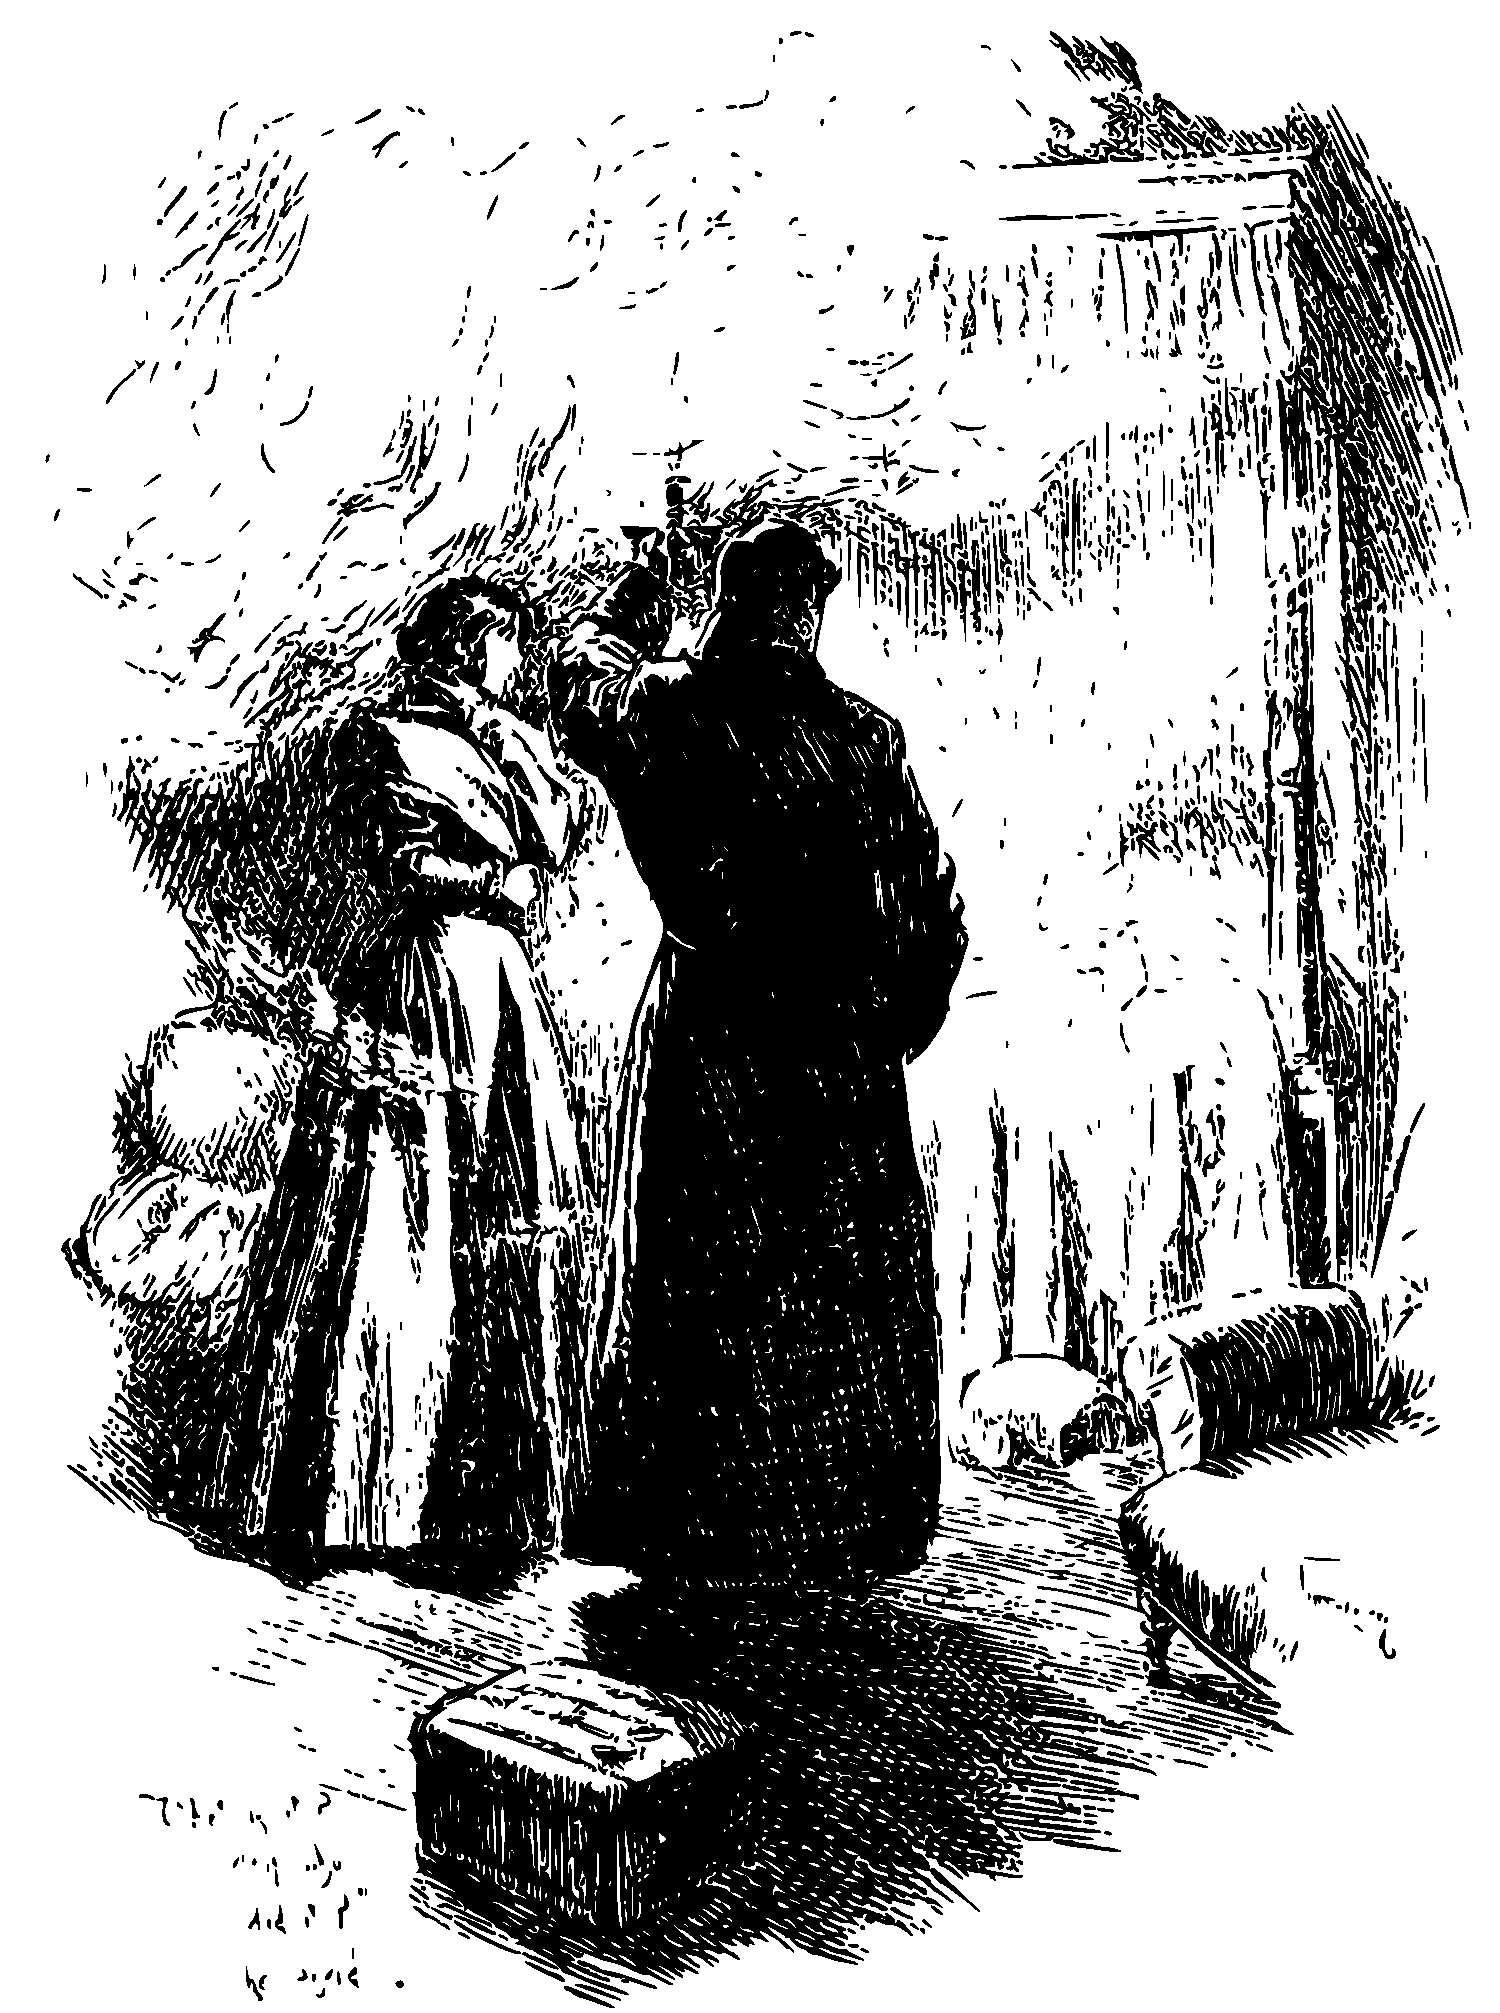
\includegraphics[width=\linewidth]{images/p140b.pdf}
	\end{sidecaption}
\end{figure}

He listened very gravely; his face, as I went on, expressed more concern
than astonishment; he did not immediately speak when I had concluded.

\enquote{Shall I call \Mrs{} Fairfax?} I asked.

\enquote{\Mrs{} Fairfax? No; what the deuce would you call her for? What
	can she do? Let her sleep unmolested.}

\enquote{Then I will fetch Leah, and wake John and his wife.}

\enquote{Not at all: just be still. You have a shawl on. If you are
	not warm enough, you may take my cloak yonder; wrap it about you, and
	sit down in the arm-chair: there,---I will put it on. Now place your
	feet on the stool, to keep them out of the wet. I am going to leave you
	a few minutes. I shall take the candle. Remain where you are till I
	return; be as still as a mouse. I must pay a visit to the second
	storey. Don't move, remember, or call any one.}

He went: I watched the light withdraw. He passed up the gallery very
softly, unclosed the staircase door with as little noise as possible,
shut it after him, and the last ray vanished. I was left in total
darkness. I listened for some noise, but heard nothing. A very long
time elapsed. I grew weary: it was cold, in spite of the cloak; and
then I did not see the use of staying, as I was not to rouse the house.
I was on the point of risking \Mr{}  Rochester's displeasure by disobeying
his orders, when the light once more gleamed dimly on the gallery wall,
and I heard his unshod feet tread the matting. \enquote{I hope it is
	he,} thought I, \enquote{and not something worse.}

He re-entered, pale and very gloomy. \enquote{I have found it all out,}
said he, setting his candle down on the washstand; \enquote{it is as I
	thought.}

\enquote{How, sir?}

He made no reply, but stood with his arms folded, looking on the
ground. At the end of a few minutes he inquired in rather a peculiar
tone---

\enquote{I forget whether you said you saw anything when you opened your
	chamber door.}

\enquote{No, sir, only the candlestick on the ground.}

\enquote{But you heard an odd laugh? You have heard that laugh before,
	I should think, or something like it?}

\enquote{Yes, sir: there is a woman who sews here, called Grace
	Poole,---she laughs in that way. She is a singular person.}

\enquote{Just so. Grace Poole---you have guessed it. She is, as you
	say, singular---very. Well, I shall reflect on the subject. Meantime,
	I am glad that you are the only person, besides myself, acquainted with
	the precise details of to-night's incident. You are no talking fool:
	say nothing about it. I will account for this state of affairs}
(pointing to the bed): \enquote{and now return to your own room. I
	shall do very well on the sofa in the library for the rest of the
	night. It is near four:---in two hours the servants will be up.}

\enquote{Good-night, then, sir,} said I, departing.

He seemed surprised---very inconsistently so, as he had just told me to
go.

\enquote{What!} he exclaimed, \enquote{are you quitting me already, and
	in that way?}

\enquote{You said I might go, sir.}

\enquote{But not without taking leave; not without a word or two of
	acknowledgment and good-will: not, in short, in that brief, dry
	fashion. Why, you have saved my life!---snatched me from a horrible and
	excruciating death! and you walk past me as if we were mutual
	strangers! At least shake hands.}

He held out his hand; I gave him mine: he took it first in one, them in
both his own.

\enquote{You have saved my life: I have a pleasure in owing you so
	immense a debt. I cannot say more. Nothing else that has being would
	have been tolerable to me in the character of creditor for such an
	obligation: but you: it is different;---I feel your benefits no burden,
	Jane.}

He paused; gazed at me: words almost visible trembled on his lips,---but
his voice was checked.

\enquote{Good-night again, sir. There is no debt, benefit, burden,
	obligation, in the case.}

\enquote{I knew,} he continued, \enquote{you would do me good in some
	way, at some time;---I saw it in your eyes when I first beheld you:
	their expression and smile did not}---(again he stopped)---\enquote{did
	not} (he proceeded hastily) \enquote{strike delight to my very inmost
	heart so for nothing. People talk of natural sympathies; I have heard
	of good genii: there are grains of truth in the wildest fable. My
	cherished preserver, goodnight!}

Strange energy was in his voice, strange fire in his look.

\enquote{I am glad I happened to be awake,} I said: and then I was
going.

\enquote{What! you \emph{will} go?}

\enquote{I am cold, sir.}

\enquote{Cold? Yes,---and standing in a pool! Go, then, Jane; go!}
But he still retained my hand, and I could not free it. I bethought
myself of an expedient.

\enquote{I think I hear \Mrs{} Fairfax move, sir,} said I\@.

\enquote{Well, leave me:} he relaxed his fingers, and I was gone.

I regained my couch, but never thought of sleep. Till morning dawned I
was tossed on a buoyant but unquiet sea, where billows of trouble rolled
under surges of joy. I thought sometimes I saw beyond its wild waters a
shore, sweet as the hills of Beulah; and now and then a freshening gale,
wakened by hope, bore my spirit triumphantly towards the bourne: but I
could not reach it, even in fancy---a counteracting breeze blew off
land, and continually drove me back. Sense would resist delirium:
judgment would warn passion. Too feverish to rest, I rose as soon as
day dawned.

\FChapter{Chapter Sixteen}{16}

\Lettrine{I}{} \textsc{both wished} and feared to see \Mr{} Rochester on the day which followed
this sleepless night: I wanted to hear his voice again, yet feared to
meet his eye.  During the early part of the morning, I momentarily
expected his coming; he was not in the frequent habit of entering the
schoolroom, but he did step in for a few minutes sometimes, and I had
the impression that he was sure to visit it that day.

But the morning passed just as usual: nothing happened to interrupt the
quiet course of Adèle's studies; only soon after breakfast, I heard some
bustle in the neighbourhood of \Mr{} Rochester's chamber, \Mrs{} Fairfax's
voice, and Leah's, and the cook's---that is, John's wife---and even
John's own gruff tones.  There were exclamations of \enquote{What a
	mercy master was not burnt in his bed!}  \enquote{It is always dangerous
	to keep a candle lit at night.}  \enquote{How providential that he had
	presence of mind to think of the water-jug!}  \enquote{I wonder he waked
	nobody!}  \enquote{It is to be hoped he will not take cold with sleeping
	on the library sofa,} \etc.

To much confabulation succeeded a sound of scrubbing and setting to
rights; and when I passed the room, in going downstairs to dinner, I saw
through the open door that all was again restored to complete order;
only the bed was stripped of its hangings.  Leah stood up in the
window-seat, rubbing the panes of glass dimmed with smoke.  I was about
to address her, for I wished to know what account had been given of the
affair: but, on advancing, I saw a second person in the chamber---a
woman sitting on a chair by the bedside, and sewing rings to new
curtains.  That woman was no other than Grace Poole.

There she sat, staid and taciturn-looking, as usual, in her brown stuff
gown, her check apron, white handkerchief, and cap.  She was intent on
her work, in which her whole thoughts seemed absorbed: on her hard
forehead, and in her commonplace features, was nothing either of the
paleness or desperation one would have expected to see marking the
countenance of a woman who had attempted murder, and whose intended
victim had followed her last night to her lair, and (as I believed),
charged her with the crime she wished to perpetrate.  I was
amazed---confounded.  She looked up, while I still gazed at her: no
start, no increase or failure of colour betrayed emotion, consciousness
of guilt, or fear of detection.  She said \enquote{Good morning, Miss,}
in her usual phlegmatic and brief manner; and taking up another ring and
more tape, went on with her sewing.

\enquote{I will put her to some test,} thought I: \enquote{such absolute
	impenetrability is past comprehension.}

\enquote{Good morning, Grace,} I said.  \enquote{Has anything happened
	here?  I thought I heard the servants all talking together a while ago.}

\enquote{Only master had been reading in his bed last night; he fell
	asleep with his candle lit, and the curtains got on fire; but,
	fortunately, he awoke before the bed-clothes or the wood-work caught,
	and contrived to quench the flames with the water in the ewer.}

\enquote{A strange affair!} I said, in a low voice: then, looking at her
fixedly---\enquote{Did \Mr{} Rochester wake nobody?  Did no one hear him
	move?}

She again raised her eyes to me, and this time there was something of
consciousness in their expression.  She seemed to examine me warily;
then she answered---

\enquote{The servants sleep so far off, you know, Miss, they would not
	be likely to hear.  \Mrs{} Fairfax's room and yours are the nearest to
	master's; but \Mrs{} Fairfax said she heard nothing: when people get
	elderly, they often sleep heavy.}  She paused, and then added, with a
sort of assumed indifference, but still in a marked and significant
tone---\enquote{But you are young, Miss; and I should say a light
	sleeper: perhaps you may have heard a noise?}

\enquote{I did,} said I, dropping my voice, so that Leah, who was still
polishing the panes, could not hear me, \enquote{and at first I thought
	it was Pilot: but Pilot cannot laugh; and I am certain I heard a laugh,
	and a strange one.}

She took a new needleful of thread, waxed it carefully, threaded her
needle with a steady hand, and then observed, with perfect composure---

\enquote{It is hardly likely master would laugh, I should think, Miss,
	when he was in such danger: You must have been dreaming.}

\enquote{I was not dreaming,} I said, with some warmth, for her brazen
coolness provoked me.  Again she looked at me; and with the same
scrutinising and conscious eye.

\enquote{Have you told master that you heard a laugh?} she inquired.

\enquote{I have not had the opportunity of speaking to him this
	morning.}

\enquote{You did not think of opening your door and looking out into the
	gallery?} she further asked.

She appeared to be cross-questioning me, attempting to draw from me
information unawares.  The idea struck me that if she discovered I knew
or suspected her guilt, she would be playing of some of her malignant
pranks on me; I thought it advisable to be on my guard.

\enquote{On the contrary,} said I, \enquote{I bolted my door.}

\enquote{Then you are not in the habit of bolting your door every night
	before you get into bed?}

\enquote{Fiend! she wants to know my habits, that she may lay her plans
	accordingly!}  Indignation again prevailed over prudence: I replied
sharply, \enquote{Hitherto I have often omitted to fasten the bolt: I
	did not think it necessary.  I was not aware any danger or annoyance was
	to be dreaded at Thornfield Hall: but in future} (and I laid marked
stress on the words) \enquote{I shall take good care to make all secure
	before I venture to lie down.}

\enquote{It will be wise so to do,} was her answer: \enquote{this
	neighbourhood is as quiet as any I know, and I never heard of the hall
	being attempted by robbers since it was a house; though there are
	hundreds of pounds' worth of plate in the plate-closet, as is well
	known.  And you see, for such a large house, there are very few
	servants, because master has never lived here much; and when he does
	come, being a bachelor, he needs little waiting on: but I always think
	it best to err on the safe side; a door is soon fastened, and it is as
	well to have a drawn bolt between one and any mischief that may be
	about.  A deal of people, Miss, are for trusting all to Providence; but
	I say Providence will not dispense with the means, though He often
	blesses them when they are used discreetly.}  And here she closed her
harangue: a long one for her, and uttered with the demureness of a
Quakeress.

I still stood absolutely dumfoundered at what appeared to me her
miraculous self-possession and most inscrutable hypocrisy, when the cook
entered.

\enquote{\Mrs{} Poole,} said she, addressing Grace, \enquote{the servants'
	dinner will soon be ready: will you come down?}

\enquote{No; just put my pint of porter and bit of pudding on a tray,
	and I'll carry it upstairs.}

\enquote{You'll have some meat?}

\enquote{Just a morsel, and a taste of cheese, that's all.}

\enquote{And the sago?}

\enquote{Never mind it at present: I shall be coming down before
	teatime: I'll make it myself.}

The cook here turned to me, saying that \Mrs{} Fairfax was waiting for me:
so I departed.

I hardly heard \Mrs{} Fairfax's account of the curtain conflagration
during dinner, so much was I occupied in puzzling my brains over the
enigmatical character of Grace Poole, and still more in pondering the
problem of her position at Thornfield and questioning why she had not
been given into custody that morning, or, at the very least, dismissed
from her master's service.  He had almost as much as declared his
conviction of her criminality last night: what mysterious cause withheld
him from accusing her?  Why had he enjoined me, too, to secrecy?  It was
strange: a bold, vindictive, and haughty gentleman seemed somehow in the
power of one of the meanest of his dependants; so much in her power,
that even when she lifted her hand against his life, he dared not openly
charge her with the attempt, much less punish her for it.

Had Grace been young and handsome, I should have been tempted to think
that tenderer feelings than prudence or fear influenced \Mr{} Rochester in
her behalf; but, hard-favoured and matronly as she was, the idea could
not be admitted.  \enquote{Yet,} I reflected, \enquote{she has been
	young once; her youth would be contemporary with her master's: \Mrs{}
	Fairfax told me once, she had lived here many years.  I don't think she
	can ever have been pretty; but, for aught I know, she may possess
	originality and strength of character to compensate for the want of
	personal advantages.  \Mr{} Rochester is an amateur of the decided and
	eccentric: Grace is eccentric at least.  What if a former caprice (a
	freak very possible to a nature so sudden and headstrong as his) has
	delivered him into her power, and she now exercises over his actions a
	secret influence, the result of his own indiscretion, which he cannot
	shake off, and dare not disregard?}  But, having reached this point of
conjecture, \Mrs{} Poole's square, flat figure, and uncomely, dry, even
coarse face, recurred so distinctly to my mind's eye, that I thought,
\enquote{No; impossible! my supposition cannot be correct.  Yet,}
suggested the secret voice which talks to us in our own hearts,
\enquote{you are not beautiful either, and perhaps \Mr{} Rochester
	approves you: at any rate, you have often felt as if he did; and last
	night---remember his words; remember his look; remember his voice!}

I well remembered all; language, glance, and tone seemed at the moment
vividly renewed.  I was now in the schoolroom; Adèle was drawing; I bent
over her and directed her pencil.  She looked up with a sort of start.

\foreignquote{french}{Qu' avez-vous, mademoiselle?} said she.  \foreignquote{french}{Vos doigts
	tremblent comme la feuille, et vos joues sont rouges: mais, rouges comme
	des cerises!}\footnote{\enquote{What's wrong, miss?} \textelp{} \enquote{Your
		fingers are trembling like leaves, and your cheeks are red: they're red as cherries!}}

\enquote{I am hot, Adèle, with stooping!}  She went on sketching; I went
on thinking.

I hastened to drive from my mind the hateful notion I had been
conceiving respecting Grace Poole; it disgusted me.  I compared myself
with her, and found we were different.  Bessie Leaven had said I was
quite a lady; and she spoke truth---I was a lady.  And now I looked much
better than I did when Bessie saw me; I had more colour and more flesh,
more life, more vivacity, because I had brighter hopes and keener
enjoyments.

\enquote{Evening approaches,} said I, as I looked towards the window.
\enquote{I have never heard \Mr{} Rochester's voice or step in the house
	to-day; but surely I shall see him before night: I feared the meeting in
	the morning; now I desire it, because expectation has been so long
	baffled that it is grown impatient.}

When dusk actually closed, and when Adèle left me to go and play in the
nursery with Sophie, I did most keenly desire it.  I listened for the
bell to ring below; I listened for Leah coming up with a message; I
fancied sometimes I heard \Mr{} Rochester's own tread, and I turned to the
door, expecting it to open and admit him.  The door remained shut;
darkness only came in through the window.  Still it was not late; he
often sent for me at seven and eight o'clock, and it was yet but six.
Surely I should not be wholly disappointed to-night, when I had so many
things to say to him!  I wanted again to introduce the subject of Grace
Poole, and to hear what he would answer; I wanted to ask him plainly if
he really believed it was she who had made last night's hideous attempt;
and if so, why he kept her wickedness a secret.  It little mattered
whether my curiosity irritated him; I knew the pleasure of vexing and
soothing him by turns; it was one I chiefly delighted in, and a sure
instinct always prevented me from going too far; beyond the verge of
provocation I never ventured; on the extreme brink I liked well to try
my skill.  Retaining every minute form of respect, every propriety of my
station, I could still meet him in argument without fear or uneasy
restraint; this suited both him and me.

A tread creaked on the stairs at last.  Leah made her appearance; but it
was only to intimate that tea was ready in \Mrs{} Fairfax's room.  Thither
I repaired, glad at least to go downstairs; for that brought me, I
imagined, nearer to \Mr{} Rochester's presence.

\enquote{You must want your tea,} said the good lady, as I joined her;
\enquote{you ate so little at dinner.  I am afraid,} she continued,
\enquote{you are not well to-day: you look flushed and feverish.}

\enquote{Oh, quite well!  I never felt better.}

\enquote{Then you must prove it by evincing a good appetite; will you
	fill the teapot while I knit off this needle?}  Having completed her
task, she rose to draw down the blind, which she had hitherto kept up,
by way, I suppose, of making the most of daylight, though dusk was now
fast deepening into total obscurity.

\enquote{It is fair to-night,} said she, as she looked through the
panes, \enquote{though not starlight; \Mr{} Rochester has, on the whole,
	had a favourable day for his journey.}

\enquote{Journey!---Is \Mr{} Rochester gone anywhere?  I did not know he
	was out.}

\enquote{Oh, he set off the moment he had breakfasted!  He is gone to
	the Leas, \Mr{} Eshton's place, ten miles on the other side Millcote.  I
	believe there is quite a party assembled there; Lord Ingram, Sir George
	Lynn, Colonel Dent, and others.}

\enquote{Do you expect him back to-night?}

\enquote{No---nor to-morrow either; I should think he is very likely to
	stay a week or more: when these fine, fashionable people get together,
	they are so surrounded by elegance and gaiety, so well provided with all
	that can please and entertain, they are in no hurry to separate.
	Gentlemen especially are often in request on such occasions; and \Mr{}
	Rochester is so talented and so lively in society, that I believe he is
	a general favourite: the ladies are very fond of him; though you would
	not think his appearance calculated to recommend him particularly in
	their eyes: but I suppose his acquirements and abilities, perhaps his
	wealth and good blood, make amends for any little fault of look.}

\enquote{Are there ladies at the Leas?}

\enquote{There are \Mrs{} Eshton and her three daughters---very elegant
	young ladies indeed; and there are the Honourable Blanche and Mary
	Ingram, most beautiful women, I suppose: indeed I have seen Blanche, six
	or seven years since, when she was a girl of eighteen.  She came here to
	a Christmas ball and party \Mr{} Rochester gave.  You should have seen the
	dining-room that day---how richly it was decorated, how brilliantly lit
	up!  I should think there were fifty ladies and gentlemen present---all
	of the first county families; and Miss Ingram was considered the belle
	of the evening.}

\enquote{You saw her, you say, \Mrs{} Fairfax: what was she like?}

\enquote{Yes, I saw her.  The dining-room doors were thrown open; and,
	as it was Christmas-time, the servants were allowed to assemble in the
	hall, to hear some of the ladies sing and play.  \Mr{} Rochester would
	have me to come in, and I sat down in a quiet corner and watched them.
	I never saw a more splendid scene: the ladies were magnificently
	dressed; most of them---at least most of the younger ones---looked
	handsome; but Miss Ingram was certainly the queen.}

\enquote{And what was she like?}

\enquote{Tall, fine bust, sloping shoulders; long, graceful neck: olive
	complexion, dark and clear; noble features; eyes rather like \Mr{}
	Rochester's: large and black, and as brilliant as her jewels.  And then
	she had such a fine head of hair; raven-black and so becomingly
	arranged: a crown of thick plaits behind, and in front the longest, the
	glossiest curls I ever saw.  She was dressed in pure white; an
	amber-coloured scarf was passed over her shoulder and across her breast,
	tied at the side, and descending in long, fringed ends below her knee.
	She wore an amber-coloured flower, too, in her hair: it contrasted well
	with the jetty mass of her curls.}

\enquote{She was greatly admired, of course?}

\enquote{Yes, indeed: and not only for her beauty, but for her
	accomplishments.  She was one of the ladies who sang: a gentleman
	accompanied her on the piano.  She and \Mr{} Rochester sang a duet.}

\enquote{\Mr{} Rochester?  I was not aware he could sing.}

\enquote{Oh! he has a fine bass voice, and an excellent taste for
	music.}

\enquote{And Miss Ingram: what sort of a voice had she?}

\enquote{A very rich and powerful one: she sang delightfully; it was a
	treat to listen to her;---and she played afterwards.  I am no judge of
	music, but \Mr{} Rochester is; and I heard him say her execution was
	remarkably good.}

\enquote{And this beautiful and accomplished lady, she is not yet
	married?}

\enquote{It appears not: I fancy neither she nor her sister have very
	large fortunes.  Old Lord Ingram's estates were chiefly entailed, and
	the eldest son came in for everything almost.}

\enquote{But I wonder no wealthy nobleman or gentleman has taken a fancy
	to her: \Mr{} Rochester, for instance.  He is rich, is he not?}

\enquote{Oh! yes.  But you see there is a considerable difference in
	age: \Mr{} Rochester is nearly forty; she is but twenty-five.}

\enquote{What of that?  More unequal matches are made every day.}

\enquote{True: yet I should scarcely fancy \Mr{} Rochester would entertain
	an idea of the sort.  But you eat nothing: you have scarcely tasted
	since you began tea.}

\enquote{No: I am too thirsty to eat.  Will you let me have another
	cup?}

I was about again to revert to the probability of a union between \Mr{}
Rochester and the beautiful Blanche; but Adèle came in, and the
conversation was turned into another channel.

When once more alone, I reviewed the information I had got; looked into
my heart, examined its thoughts and feelings, and endeavoured to bring
back with a strict hand such as had been straying through imagination's
boundless and trackless waste, into the safe fold of common sense.

Arraigned at my own bar, Memory having given her evidence of the hopes,
wishes, sentiments I had been cherishing since last night---of the
general state of mind in which I had indulged for nearly a fortnight
past; Reason having come forward and told, in her own quiet way a plain,
unvarnished tale, showing how I had rejected the real, and rabidly
devoured the ideal;---I pronounced judgment to this effect:---

That a greater fool than Jane Eyre had never breathed the breath of
life; that a more fantastic idiot had never surfeited herself on sweet
lies, and swallowed poison as if it were nectar.

\enquote{\emph{You},} I said, \enquote{a favourite with \Mr{} Rochester?  \emph{You}
	gifted with the power of pleasing him?  \emph{You} of importance to him
	in any way?  Go! your folly sickens me.  And you have derived pleasure
	from occasional tokens of preference---equivocal tokens shown by a
	gentleman of family and a man of the world to a dependent and a novice.
	How dared you?  Poor stupid dupe!---Could not even self-interest make
	you wiser? You repeated to yourself this morning the brief scene of last
	night?---Cover your face and be ashamed!  He said something in praise of
	your eyes, did he?  Blind puppy!  Open their bleared lids and look on
	your own accursed senselessness!  It does good to no woman to be
	flattered by her superior, who cannot possibly intend to marry her; and
	it is madness in all women to let a secret love kindle within them,
	which, if unreturned and unknown, must devour the life that feeds it;
	and, if discovered and responded to, must lead,
	\emph{ignis-fatuus}-like, into miry wilds whence there is no
	extrication.

	%rem enq
	Listen, then, Jane Eyre, to your sentence: to-morrow, place the glass
	before you, and draw in chalk your own picture, faithfully, without
	softening one defect; omit no harsh line, smooth away no displeasing
	irregularity; write under it, \enquote{Portrait of a Governess,
		disconnected, poor, and plain.}

	%rem enq
	Afterwards, take a piece of smooth ivory---you have one prepared in
	your drawing-box: take your palette, mix your freshest, finest, clearest
	tints; choose your most delicate camel-hair pencils; delineate carefully
	the loveliest face you can imagine; paint it in your softest shades and
	sweetest lines, according to the description given by \Mrs{} Fairfax of
	Blanche Ingram; remember the raven ringlets, the oriental eye;---What!
	you revert to \Mr{} Rochester as a model!  Order!  No snivel!---no
	sentiment!---no regret!  I will endure only sense and resolution.
	Recall the august yet harmonious lineaments, the Grecian neck and bust;
	let the round and dazzling arm be visible, and the delicate hand; omit
	neither diamond ring nor gold bracelet; portray faithfully the attire,
	aërial lace and glistening satin, graceful scarf and golden rose; call
	it \enquote{Blanche, an accomplished lady of rank.}

	%rem enq
	Whenever, in future, you should chance to fancy \Mr{} Rochester
	thinks well of you, take out these two pictures and compare them: say,
	\enquote{\Mr{} Rochester might probably win that noble lady's love, if he
		chose to strive for it; is it likely he would waste a serious thought on
		this indigent and insignificant plebeian?}}

\enquote{I'll do it,} I resolved: and having framed this determination,
I grew calm, and fell asleep.

I kept my word.  An hour or two sufficed to sketch my own portrait in
crayons; and in less than a fortnight I had completed an ivory miniature
of an imaginary Blanche Ingram.  It looked a lovely face enough, and
when compared with the real head in chalk, the contrast was as great as
self-control could desire.  I derived benefit from the task: it had kept
my head and hands employed, and had given force and fixedness to the new
impressions I wished to stamp indelibly on my heart.

Ere long, I had reason to congratulate myself on the course of wholesome
discipline to which I had thus forced my feelings to submit.  Thanks to
it, I was able to meet subsequent occurrences with a decent calm, which,
had they found me unprepared, I should probably have been unequal to
maintain, even externally.

\FChapter{Chapter Seventeen}{17}

\Lettrine{A}{} \textsc{week passed,} and no news arrived of \Mr{} Rochester: ten days, and still
he did not come. \Mrs{} Fairfax said she should not be surprised if he
were to go straight from the Leas to London, and thence to the
Continent, and not show his face again at Thornfield for a year to come;
he had not unfrequently quitted it in a manner quite as abrupt and
unexpected. When I heard this, I was beginning to feel a strange chill
and failing at the heart. I was actually permitting myself to
experience a sickening sense of disappointment; but rallying my wits,
and recollecting my principles, I at once called my sensations to order;
and it was wonderful how I got over the temporary blunder---how I
cleared up the mistake of supposing \Mr{} Rochester's movements a matter
in which I had any cause to take a vital interest. Not that I humbled
myself by a slavish notion of inferiority: on the contrary, I just
said---

\enquote{You have nothing to do with the master of Thornfield, further
than to receive the salary he gives you for teaching his protégée, and
to be grateful for such respectful and kind treatment as, if you do your
duty, you have a right to expect at his hands. Be sure that is the only
tie he seriously acknowledges between you and him; so don't make him the
object of your fine feelings, your raptures, agonies, and so forth. He
is not of your order: keep to your caste, and be too self-respecting to
lavish the love of the whole heart, soul, and strength, where such a
gift is not wanted and would be despised.}

I went on with my day's business tranquilly; but ever and anon vague
suggestions kept wandering across my brain of reasons why I should quit
Thornfield; and I kept involuntarily framing advertisements and
pondering conjectures about new situations: these thoughts I did not
think to check; they might germinate and bear fruit if they could.

\Mr{} Rochester had been absent upwards of a fortnight, when the post
brought \Mrs{} Fairfax a letter.

\enquote{It is from the master,} said she, as she looked at the
direction. \enquote{Now I suppose we shall know whether we are to
expect his return or not.}

And while she broke the seal and perused the document, I went on taking
my coffee (we were at breakfast): it was hot, and I attributed to that
circumstance a fiery glow which suddenly rose to my face. Why my hand
shook, and why I involuntarily spilt half the contents of my cup into my
saucer, I did not choose to consider.

\enquote{Well, I sometimes think we are too quiet; but we run a chance
of being busy enough now: for a little while at least,} said \Mrs{}
Fairfax, still holding the note before her spectacles.

Ere I permitted myself to request an explanation, I tied the string of
Adèle's pinafore, which happened to be loose: having helped her also to
another bun and refilled her mug with milk, I said, nonchalantly---

\enquote{\Mr{} Rochester is not likely to return soon, I suppose?}

\enquote{Indeed he is---in three days, he says: that will be next
Thursday; and not alone either. I don't know how many of the fine
people at the Leas are coming with him: he sends directions for all the
best bedrooms to be prepared; and the library and drawing-rooms are to
be cleaned out; I am to get more kitchen hands from the George Inn, at
Millcote, and from wherever else I can; and the ladies will bring their
maids and the gentlemen their valets: so we shall have a full house of
it.} And \Mrs{} Fairfax swallowed her breakfast and hastened away to
commence operations.

The three days were, as she had foretold, busy enough. I had thought
all the rooms at Thornfield beautifully clean and well arranged; but it
appears I was mistaken. Three women were got to help; and such
scrubbing, such brushing, such washing of paint and beating of carpets,
such taking down and putting up of pictures, such polishing of mirrors
and lustres, such lighting of fires in bedrooms, such airing of sheets
and feather-beds on hearths, I never beheld, either before or since. 
Adèle ran quite wild in the midst of it: the preparations for company
and the prospect of their arrival, seemed to throw her into ecstasies. 
She would have Sophie to look over all her \foreignquote{french}{toilettes,} as she
called frocks; to furbish up any that were \foreignquote{french}{\emph{passées},} and to
air and arrange the new. For herself, she did nothing but caper about
in the front chambers, jump on and off the bedsteads, and lie on the
mattresses and piled-up bolsters and pillows before the enormous fires
roaring in the chimneys. From school duties she was exonerated: \Mrs{}
Fairfax had pressed me into her service, and I was all day in the
storeroom, helping (or hindering) her and the cook; learning to make
custards and cheese-cakes and French pastry, to truss game and garnish
desert-dishes.

The party were expected to arrive on Thursday afternoon, in time for
dinner at six. During the intervening period I had no time to nurse
chimeras; and I believe I was as active and gay as anybody---Adèle
excepted. Still, now and then, I received a damping check to my
cheerfulness; and was, in spite of myself, thrown back on the region of
doubts and portents, and dark conjectures. This was when I chanced to
see the third-storey staircase door (which of late had always been kept
locked) open slowly, and give passage to the form of Grace Poole, in
prim cap, white apron, and handkerchief; when I watched her glide along
the gallery, her quiet tread muffled in a list slipper; when I saw her
look into the bustling, topsy-turvy bedrooms,---just say a word,
perhaps, to the charwoman about the proper way to polish a grate, or
clean a marble mantelpiece, or take stains from papered walls, and then
pass on. She would thus descend to the kitchen once a day, eat her
dinner, smoke a moderate pipe on the hearth, and go back, carrying her
pot of porter with her, for her private solace, in her own gloomy, upper
haunt. Only one hour in the twenty-four did she pass with her
fellow-servants below; all the rest of her time was spent in some
low-ceiled, oaken chamber of the second storey: there she sat and
sewed---and probably laughed drearily to herself,---as companionless as
a prisoner in his dungeon.

The strangest thing of all was, that not a soul in the house, except me,
noticed her habits, or seemed to marvel at them: no one discussed her
position or employment; no one pitied her solitude or isolation. I
once, indeed, overheard part of a dialogue between Leah and one of the
charwomen, of which Grace formed the subject. Leah had been saying
something I had not caught, and the charwoman remarked---

\enquote{She gets good wages, I guess?}

\enquote{Yes,} said Leah; \enquote{I wish I had as good; not that mine
are to complain of,---there's no stinginess at Thornfield; but they're
not one fifth of the sum \Mrs{} Poole receives. And she is laying by: she
goes every quarter to the bank at Millcote. I should not wonder but she
has saved enough to keep her independent if she liked to leave; but I
suppose she's got used to the place; and then she's not forty yet, and
strong and able for anything. It is too soon for her to give up
business.}

\enquote{She is a good hand, I daresay,} said the charwoman.

\enquote{Ah!---she understands what she has to do,---nobody better,}
rejoined Leah significantly; \enquote{and it is not every one could fill
her shoes---not for all the money she gets.}

\enquote{That it is not!} was the reply. \enquote{I wonder whether the
master---}

The charwoman was going on; but here Leah turned and perceived me, and
she instantly gave her companion a nudge.

\enquote{Doesn't she know?} I heard the woman whisper.

Leah shook her head, and the conversation was of course dropped. All I
had gathered from it amounted to this,---that there was a mystery at
Thornfield; and that from participation in that mystery I was purposely
excluded.

Thursday came: all work had been completed the previous evening; carpets
were laid down, bed-hangings festooned, radiant white counterpanes
spread, toilet tables arranged, furniture rubbed, flowers piled in
vases: both chambers and saloons looked as fresh and bright as hands
could make them. The hall, too, was scoured; and the great carved
clock, as well as the steps and banisters of the staircase, were
polished to the brightness of glass; in the dining-room, the sideboard
flashed resplendent with plate; in the drawing-room and boudoir, vases
of exotics bloomed on all sides.

Afternoon arrived: \Mrs{} Fairfax assumed her best black satin gown, her
gloves, and her gold watch; for it was her part to receive the
company,---to conduct the ladies to their rooms, \etc. Adèle, too, would
be dressed: though I thought she had little chance of being introduced
to the party that day at least. However, to please her, I allowed
Sophie to apparel her in one of her short, full muslin frocks. For
myself, I had no need to make any change; I should not be called upon to
quit my sanctum of the schoolroom; for a sanctum it was now become to
me,---\enquote{a very pleasant refuge in time of trouble.}

It had been a mild, serene spring day---one of those days which, towards
the end of March or the beginning of April, rise shining over the earth
as heralds of summer. It was drawing to an end now; but the evening was
even warm, and I sat at work in the schoolroom with the window open.

\enquote{It gets late,} said \Mrs{} Fairfax, entering in rustling state. 
\enquote{I am glad I ordered dinner an hour after the time \Mr{} Rochester
mentioned; for it is past six now. I have sent John down to the gates
to see if there is anything on the road: one can see a long way from
thence in the direction of Millcote.} She went to the window. 
\enquote{Here he is!} said she. \enquote{Well, John} (leaning out),
\enquote{any news?}

\enquote{They're coming, ma'am,} was the answer. \enquote{They'll be
here in ten minutes.}

Adèle flew to the window. I followed, taking care to stand on one side,
so that, screened by the curtain, I could see without being seen.

The ten minutes John had given seemed very long, but at last wheels were
heard; four equestrians galloped up the drive, and after them came two
open carriages. Fluttering veils and waving plumes filled the vehicles;
two of the cavaliers were young, dashing-looking gentlemen; the third
was \Mr{} Rochester, on his black horse, Mesrour, Pilot bounding before
him; at his side rode a lady, and he and she were the first of the
party. Her purple riding-habit almost swept the ground, her veil
streamed long on the breeze; mingling with its transparent folds, and
gleaming through them, shone rich raven ringlets.

\enquote{Miss Ingram!} exclaimed \Mrs{} Fairfax, and away she hurried to
her post below.

The cavalcade, following the sweep of the drive, quickly turned the
angle of the house, and I lost sight of it. Adèle now petitioned to go
down; but I took her on my knee, and gave her to understand that she
must not on any account think of venturing in sight of the ladies,
either now or at any other time, unless expressly sent for: that \Mr{}
 Rochester would be very angry, \etc. \enquote{Some natural tears she
shed} on being told this; but as I began to look very grave, she
consented at last to wipe them.

A joyous stir was now audible in the hall: gentlemen's deep tones and
ladies' silvery accents blent harmoniously together, and distinguishable
above all, though not loud, was the sonorous voice of the master of
Thornfield Hall, welcoming his fair and gallant guests under its roof. 
Then light steps ascended the stairs; and there was a tripping through
the gallery, and soft cheerful laughs, and opening and closing doors,
and, for a time, a hush.

\foreignquote{french}{Elles changent de toilettes,}\footnote{\enquote{They are changing their clothes.}} 
said Adèle; who, listening attentively, had followed every movement; and she sighed.

\foreignquote{french}{Chez maman,} said she, \foreignquote{french}{quand il y avait du monde, je
le suivais partout, au salon et à leurs chambres; souvent je regardais
les femmes de chambre coiffer et habiller les dames, et c'était si
amusant: comme cela on apprend.}\footnote{\enquote{At my mother's,} \textelp{}
\enquote{when there were guests, I used to follow them everywhere, from the
drawing room to their bedrooms; often I used to watch the maids arrange
the ladies' hair and dress them, and that was so interesting: you can
learn from that.}}

\enquote{Don't you feel hungry, Adèle?}

\foreignquote{french}{Mais oui, mademoiselle: voilà cinq ou six heures que nous
n'avons pas mangé.}\footnote{\enquote{Oh yes, miss: it's been five or six hours since we've eaten.}}

\enquote{Well now, while the ladies are in their rooms, I will venture
down and get you something to eat.}

And issuing from my asylum with precaution, I sought a back-stairs which
conducted directly to the kitchen. All in that region was fire and
commotion; the soup and fish were in the last stage of projection, and
the cook hung over her crucibles in a frame of mind and body threatening
spontaneous combustion. In the servants' hall two coachmen and three
gentlemen's gentlemen stood or sat round the fire; the abigails, I
suppose, were upstairs with their mistresses; the new servants, that had
been hired from Millcote, were bustling about everywhere. Threading
this chaos, I at last reached the larder; there I took possession of a
cold chicken, a roll of bread, some tarts, a plate or two and a knife
and fork: with this booty I made a hasty retreat. I had regained the
gallery, and was just shutting the back-door behind me, when an
accelerated hum warned me that the ladies were about to issue from their
chambers. I could not proceed to the schoolroom without passing some of
their doors, and running the risk of being surprised with my cargo of
victualage; so I stood still at this end, which, being windowless, was
dark: quite dark now, for the sun was set and twilight gathering.

Presently the chambers gave up their fair tenants one after another:
each came out gaily and airily, with dress that gleamed lustrous through
the dusk. For a moment they stood grouped together at the other
extremity of the gallery, conversing in a key of sweet subdued vivacity:
they then descended the staircase almost as noiselessly as a bright mist
rolls down a hill. Their collective appearance had left on me an
impression of high-born elegance, such as I had never before received.

I found Adèle peeping through the schoolroom door, which she held ajar. 
\enquote{What beautiful ladies!} cried she in English. \enquote{Oh, I
wish I might go to them! Do you think \Mr{} Rochester will send for us
by-and-bye, after dinner?}

\enquote{No, indeed, I don't; \Mr{} Rochester has something else to think
about. Never mind the ladies to-night; perhaps you will see them
to-morrow: here is your dinner.}

She was really hungry, so the chicken and tarts served to divert her
attention for a time. It was well I secured this forage, or both she,
I, and Sophie, to whom I conveyed a share of our repast, would have run
a chance of getting no dinner at all: every one downstairs was too much
engaged to think of us. The dessert was not carried out till after nine
and at ten footmen were still running to and fro with trays and
coffee-cups. I allowed Adèle to sit up much later than usual; for she
declared she could not possibly go to sleep while the doors kept opening
and shutting below, and people bustling about. Besides, she added, a
message might possibly come from \Mr{} Rochester when she was undressed;
\foreignquote{french}{et alors quel dommage!}\footnote{\enquote{And then what a shame!}}

I told her stories as long as she would listen to them; and then for a
change I took her out into the gallery. The hall lamp was now lit, and
it amused her to look over the balustrade and watch the servants passing
backwards and forwards. When the evening was far advanced, a sound of
music issued from the drawing-room, whither the piano had been removed;
Adèle and I sat down on the top step of the stairs to listen. Presently
a voice blent with the rich tones of the instrument; it was a lady who
sang, and very sweet her notes were. The solo over, a duet followed,
and then a glee: a joyous conversational murmur filled up the
intervals. I listened long: suddenly I discovered that my ear was
wholly intent on analysing the mingled sounds, and trying to
discriminate amidst the confusion of accents those of \Mr{} Rochester; and
when it caught them, which it soon did, it found a further task in
framing the tones, rendered by distance inarticulate, into words.

The clock struck eleven. I looked at Adèle, whose head leant against my
shoulder; her eyes were waxing heavy, so I took her up in my arms and
carried her off to bed. It was near one before the gentlemen and ladies
sought their chambers.

The next day was as fine as its predecessor: it was devoted by the party
to an excursion to some site in the neighbourhood. They set out early
in the forenoon, some on horseback, the rest in carriages; I witnessed
both the departure and the return. Miss Ingram, as before, was the only
lady equestrian; and, as before, \Mr{} Rochester galloped at her side; the
two rode a little apart from the rest. I pointed out this circumstance
to \Mrs{} Fairfax, who was standing at the window with me---

\enquote{You said it was not likely they should think of being married,}
said I, \enquote{but you see \Mr{} Rochester evidently prefers her to any
of the other ladies.}

\enquote{Yes, I daresay: no doubt he admires her.}

\enquote{And she him,} I added; \enquote{look how she leans her head
towards him as if she were conversing confidentially; I wish I could see
her face; I have never had a glimpse of it yet.}

\enquote{You will see her this evening,} answered \Mrs{} Fairfax. 
\enquote{I happened to remark to \Mr{} Rochester how much Adèle wished to
be introduced to the ladies, and he said: \enquote{Oh! let her come
into the drawing-room after dinner; and request Miss Eyre to accompany
her.}}

\enquote{Yes; he said that from mere politeness: I need not go, I am
sure,} I answered.

\enquote{Well, I observed to him that as you were unused to company, I
did not think you would like appearing before so gay a party---all
strangers; and he replied, in his quick way---\enquote{Nonsense! If she
objects, tell her it is my particular wish; and if she resists, say I
shall come and fetch her in case of contumacy.}}

\enquote{I will not give him that trouble,} I answered. \enquote{I will
go, if no better may be; but I don't like it. Shall you be there, \Mrs{}
Fairfax?}

\enquote{No; I pleaded off, and he admitted my plea. I'll tell you how
to manage so as to avoid the embarrassment of making a formal entrance,
which is the most disagreeable part of the business. You must go into
the drawing-room while it is empty, before the ladies leave the
dinner-table; choose your seat in any quiet nook you like; you need not
stay long after the gentlemen come in, unless you please: just let \Mr{}
 Rochester see you are there and then slip away---nobody will notice
you.}

\enquote{Will these people remain long, do you think?}

\enquote{Perhaps two or three weeks, certainly not more. After the
Easter recess, Sir George Lynn, who was lately elected member for
Millcote, will have to go up to town and take his seat; I daresay \Mr{}
 Rochester will accompany him: it surprises me that he has already made
so protracted a stay at Thornfield.}

It was with some trepidation that I perceived the hour approach when I
was to repair with my charge to the drawing-room. Adèle had been in a
state of ecstasy all day, after hearing she was to be presented to the
ladies in the evening; and it was not till Sophie commenced the
operation of dressing her that she sobered down. Then the importance of
the process quickly steadied her, and by the time she had her curls
arranged in well-smoothed, drooping clusters, her pink satin frock put
on, her long sash tied, and her lace mittens adjusted, she looked as
grave as any judge. No need to warn her not to disarrange her attire:
when she was dressed, she sat demurely down in her little chair, taking
care previously to lift up the satin skirt for fear she should crease
it, and assured me she would not stir thence till I was ready. This I
quickly was: my best dress (the silver-grey one, purchased for Miss
Temple's wedding, and never worn since) was soon put on; my hair was
soon smoothed; my sole ornament, the pearl brooch, soon assumed. We
descended.

Fortunately there was another entrance to the drawing-room than that
through the saloon where they were all seated at dinner. We found the
apartment vacant; a large fire burning silently on the marble hearth,
and wax candles shining in bright solitude, amid the exquisite flowers
with which the tables were adorned. The crimson curtain hung before the
arch: slight as was the separation this drapery formed from the party in
the adjoining saloon, they spoke in so low a key that nothing of their
conversation could be distinguished beyond a soothing murmur.

Adèle, who appeared to be still under the influence of a most
solemnising impression, sat down, without a word, on the footstool I
pointed out to her. I retired to a window-seat, and taking a book from
a table near, endeavoured to read. Adèle brought her stool to my feet;
ere long she touched my knee.

\enquote{What is it, Adèle?}

\foreignquote{french}{Est-ce que je ne puis pas prendrie une seule de ces fleurs
magnifiques, mademoiselle? Seulement pour completer ma toilette.}\footnote{
\enquote{May I take one of these glorious flowers, miss? Just to complete my outfit.}}

\enquote{You think too much of your \foreignquote{french}{toilette,} Adèle: but you
may have a flower.} And I took a rose from a vase and fastened it in
her sash. She sighed a sigh of ineffable satisfaction, as if her cup of
happiness were now full. I turned my face away to conceal a smile I
could not suppress: there was something ludicrous as well as painful in
the little Parisienne's earnest and innate devotion to matters of dress.

A soft sound of rising now became audible; the curtain was swept back
from the arch; through it appeared the dining-room, with its lit lustre
pouring down light on the silver and glass of a magnificent
dessert-service covering a long table; a band of ladies stood in the
opening; they entered, and the curtain fell behind them.

There were but eight; yet, somehow, as they flocked in, they gave the
impression of a much larger number. Some of them were very tall; many
were dressed in white; and all had a sweeping amplitude of array that
seemed to magnify their persons as a mist magnifies the moon. I rose
and curtseyed to them: one or two bent their heads in return, the others
only stared at me.

They dispersed about the room, reminding me, by the lightness and
buoyancy of their movements, of a flock of white plumy birds. Some of
them threw themselves in half-reclining positions on the sofas and
ottomans: some bent over the tables and examined the flowers and books:
the rest gathered in a group round the fire: all talked in a low but
clear tone which seemed habitual to them. I knew their names
afterwards, and may as well mention them now.

First, there was \Mrs{} Eshton and two of her daughters. She had
evidently been a handsome woman, and was well preserved still. Of her
daughters, the eldest, Amy, was rather little: naive, and child-like in
face and manner, and piquant in form; her white muslin dress and blue
sash became her well. The second, Louisa, was taller and more elegant
in figure; with a very pretty face, of that order the French term
\foreignlanguage{french}{\emph{minois chiffoné:}}\footnote{
	Literally \emph{\enquote{crumpled little face;}} someone who is attractive in an unusual way.} both sisters were fair as lilies. %TODO include colon?

Lady Lynn was a large and stout personage of about forty, very erect,
very haughty-looking, richly dressed in a satin robe of changeful sheen:
her dark hair shone glossily under the shade of an azure plume, and
within the circlet of a band of gems.

\Mrs{} Colonel Dent was less showy; but, I thought, more lady-like. She
had a slight figure, a pale, gentle face, and fair hair. Her black
satin dress, her scarf of rich foreign lace, and her pearl ornaments,
pleased me better than the rainbow radiance of the titled dame.

But the three most distinguished---partly, perhaps, because the tallest
figures of the band---were the Dowager Lady Ingram and her daughters,
Blanche and Mary. They were all three of the loftiest stature of
women. The Dowager might be between forty and fifty: her shape was
still fine; her hair (by candle-light at least) still black; her teeth,
too, were still apparently perfect. Most people would have termed her a
splendid woman of her age: and so she was, no doubt, physically
speaking; but then there was an expression of almost insupportable
haughtiness in her bearing and countenance. She had Roman features and
a double chin, disappearing into a throat like a pillar: these features
appeared to me not only inflated and darkened, but even furrowed with
pride; and the chin was sustained by the same principle, in a position
of almost preternatural erectness. She had, likewise, a fierce and a
hard eye: it reminded me of \Mrs{} Reed's; she mouthed her words in
speaking; her voice was deep, its inflections very pompous, very
dogmatical,---very intolerable, in short. A crimson velvet robe, and a
shawl turban of some gold-wrought Indian fabric, invested her (I suppose
she thought) with a truly imperial dignity.

Blanche and Mary were of equal stature,---straight and tall as poplars. 
Mary was too slim for her height, but Blanche was moulded like a Dian. 
I regarded her, of course, with special interest. First, I wished to
see whether her appearance accorded with \Mrs{} Fairfax's description;
secondly, whether it at all resembled the fancy miniature I had painted
of her; and thirdly---it will out!---whether it were such as I should
fancy likely to suit \Mr{} Rochester's taste.

As far as person went, she answered point for point, both to my picture
and \Mrs{} Fairfax's description. The noble bust, the sloping shoulders,
the graceful neck, the dark eyes and black ringlets were all
there;---but her face? Her face was like her mother's; a youthful
unfurrowed likeness: the same low brow, the same high features, the same
pride. It was not, however, so saturnine a pride! she laughed
continually; her laugh was satirical, and so was the habitual expression
of her arched and haughty lip.

Genius is said to be self-conscious. I cannot tell whether Miss Ingram
was a genius, but she was self-conscious---remarkably self-conscious
indeed. She entered into a discourse on botany with the gentle \Mrs{}
Dent. It seemed \Mrs{} Dent had not studied that science: though, as she
said, she liked flowers, \enquote{especially wild ones;} Miss Ingram
had, and she ran over its vocabulary with an air. I presently perceived
she was (what is vernacularly termed) \emph{trailing} \Mrs{} Dent; that
is, playing on her ignorance---her \emph{trail} might be clever, but it
was decidedly not good-natured. She played: her execution was
brilliant; she sang: her voice was fine; she talked French apart to her
mamma; and she talked it well, with fluency and with a good accent.

Mary had a milder and more open countenance than Blanche; softer
features too, and a skin some shades fairer (Miss Ingram was dark as a
Spaniard)---but Mary was deficient in life: her face lacked expression,
her eye lustre; she had nothing to say, and having once taken her seat,
remained fixed like a statue in its niche. The sisters were both
attired in spotless white.

And did I now think Miss Ingram such a choice as \Mr{} Rochester would be
likely to make? I could not tell---I did not know his taste in female
beauty. If he liked the majestic, she was the very type of majesty:
then she was accomplished, sprightly. Most gentlemen would admire her,
I thought; and that he \emph{did} admire her, I already seemed to have
obtained proof: to remove the last shade of doubt, it remained but to
see them together.

You are not to suppose, reader, that Adèle has all this time been
sitting motionless on the stool at my feet: no; when the ladies entered,
she rose, advanced to meet them, made a stately reverence, and said with
gravity---

\foreignquote{french}{Bon jour, mesdames.}

And Miss Ingram had looked down at her with a mocking air, and
exclaimed, \enquote{Oh, what a little puppet!}

Lady Lynn had remarked, \enquote{It is \Mr{} Rochester's ward, I
suppose---the little French girl he was speaking of.}

\Mrs{} Dent had kindly taken her hand, and given her a kiss.

Amy and Louisa Eshton had cried out simultaneously---\enquote{What a
love of a child!}

And then they had called her to a sofa, where she now sat, ensconced
between them, chattering alternately in French and broken English;
absorbing not only the young ladies' attention, but that of \Mrs{} Eshton
and Lady Lynn, and getting spoilt to her heart's content.

At last coffee is brought in, and the gentlemen are summoned. I sit in
the shade---if any shade there be in this brilliantly-lit apartment; the
window-curtain half hides me. Again the arch yawns; they come. The
collective appearance of the gentlemen, like that of the ladies, is very
imposing: they are all costumed in black; most of them are tall, some
young. Henry and Frederick Lynn are very dashing sparks indeed; and
Colonel Dent is a fine soldierly man. \Mr{} Eshton, the magistrate of the
district, is gentleman-like: his hair is quite white, his eyebrows and
whiskers still dark, which gives him something of the appearance of a
\foreignquote{french}{père noble de théâtre.}\footnote{
	\enquote{A father of the theatre.}} Lord Ingram, like his sisters, is very
tall; like them, also, he is handsome; but he shares Mary's apathetic
and listless look: he seems to have more length of limb than vivacity of
blood or vigour of brain.

And where is \Mr{} Rochester?

He comes in last: I am not looking at the arch, yet I see him enter. I
try to concentrate my attention on those netting-needles, on the meshes
of the purse I am forming---I wish to think only of the work I have in
my hands, to see only the silver beads and silk threads that lie in my
lap; whereas, I distinctly behold his figure, and I inevitably recall
the moment when I last saw it; just after I had rendered him, what he
deemed, an essential service, and he, holding my hand, and looking down
on my face, surveyed me with eyes that revealed a heart full and eager
to overflow; in whose emotions I had a part. How near had I approached
him at that moment! What had occurred since, calculated to change his
and my relative positions? Yet now, how distant, how far estranged we
were! So far estranged, that I did not expect him to come and speak to
me. I did not wonder, when, without looking at me, he took a seat at
the other side of the room, and began conversing with some of the
ladies.

No sooner did I see that his attention was riveted on them, and that I
might gaze without being observed, than my eyes were drawn involuntarily
to his face; I could not keep their lids under control: they would rise,
and the irids would fix on him. I looked, and had an acute pleasure in
looking,---a precious yet poignant pleasure; pure gold, with a steely
point of agony: a pleasure like what the thirst-perishing man might feel
who knows the well to which he has crept is poisoned, yet stoops and
drinks divine draughts nevertheless.

Most true is it that \enquote{beauty is in the eye of the gazer.} My
master's colourless, olive face, square, massive brow, broad and jetty
eyebrows, deep eyes, strong features, firm, grim mouth,---all energy,
decision, will,---were not beautiful, according to rule; but they were
more than beautiful to me; they were full of an interest, an influence
that quite mastered me,---that took my feelings from my own power and
fettered them in his. I had not intended to love him; the reader knows
I had wrought hard to extirpate from my soul the germs of love there
detected; and now, at the first renewed view of him, they spontaneously
arrived, green and strong! He made me love him without looking at me.

I compared him with his guests. What was the gallant grace of the
Lynns, the languid elegance of Lord Ingram,---even the military
distinction of Colonel Dent, contrasted with his look of native pith and
genuine power? I had no sympathy in their appearance, their expression:
yet I could imagine that most observers would call them attractive,
handsome, imposing; while they would pronounce \Mr{} Rochester at once
harsh-featured and melancholy-looking. I saw them smile, laugh---it was
nothing; the light of the candles had as much soul in it as their smile;
the tinkle of the bell as much significance as their laugh. I saw \Mr{}
 Rochester smile:---his stern features softened; his eye grew both
brilliant and gentle, its ray both searching and sweet. He was talking,
at the moment, to Louisa and Amy Eshton. I wondered to see them receive
with calm that look which seemed to me so penetrating: I expected their
eyes to fall, their colour to rise under it; yet I was glad when I found
they were in no sense moved. \enquote{He is not to them what he is to
me,} I thought: \enquote{he is not of their kind. I believe he is of
mine;---I am sure he is---I feel akin to him---I understand the language
of his countenance and movements: though rank and wealth sever us
widely, I have something in my brain and heart, in my blood and nerves,
that assimilates me mentally to him. Did I say, a few days since, that
I had nothing to do with him but to receive my salary at his hands? Did
I forbid myself to think of him in any other light than as a paymaster? 
Blasphemy against nature! Every good, true, vigorous feeling I have
gathers impulsively round him. I know I must conceal my sentiments: I
must smother hope; I must remember that he cannot care much for me. For
when I say that I am of his kind, I do not mean that I have his force to
influence, and his spell to attract; I mean only that I have certain
tastes and feelings in common with him. I must, then, repeat
continually that we are for ever sundered:---and yet, while I breathe
and think, I must love him.}

Coffee is handed. The ladies, since the gentlemen entered, have become
lively as larks; conversation waxes brisk and merry. Colonel Dent and
\Mr{} Eshton argue on politics; their wives listen. The two proud
dowagers, Lady Lynn and Lady Ingram, confabulate together. Sir
George---whom, by-the-bye, I have forgotten to describe,---a very big,
and very fresh-looking country gentleman, stands before their sofa,
coffee-cup in hand, and occasionally puts in a word. \Mr{} Frederick Lynn
has taken a seat beside Mary Ingram, and is showing her the engravings
of a splendid volume: she looks, smiles now and then, but apparently
says little. The tall and phlegmatic Lord Ingram leans with folded arms
on the chair-back of the little and lively Amy Eshton; she glances up at
him, and chatters like a wren: she likes him better than she does \Mr{}
 Rochester. Henry Lynn has taken possession of an ottoman at the feet of
Louisa: Adèle shares it with him: he is trying to talk French with her,
and Louisa laughs at his blunders. With whom will Blanche Ingram pair? 
She is standing alone at the table, bending gracefully over an album. 
She seems waiting to be sought; but she will not wait too long: she
herself selects a mate.

\Mr{} Rochester, having quitted the Eshtons, stands on the hearth as
solitary as she stands by the table: she confronts him, taking her
station on the opposite side of the mantelpiece.

\enquote{\Mr{} Rochester, I thought you were not fond of children?}

\enquote{Nor am I\@.}

\enquote{Then, what induced you to take charge of such a little doll as
that?} (pointing to Adèle). \enquote{Where did you pick her up?}

\enquote{I did not pick her up; she was left on my hands.}

\enquote{You should have sent her to school.}

\enquote{I could not afford it: schools are so dear.}

\enquote{Why, I suppose you have a governess for her: I saw a person
with her just now---is she gone? Oh, no! there she is still, behind the
window-curtain. You pay her, of course; I should think it quite as
expensive,---more so; for you have them both to keep in addition.}

I feared---or should I say, hoped?---the allusion to me would make \Mr{}
 Rochester glance my way; and I involuntarily shrank farther into the
shade: but he never turned his eyes.

\enquote{I have not considered the subject,} said he indifferently,
looking straight before him.

\enquote{No, you men never do consider economy and common sense. You
should hear mama on the chapter of governesses: Mary and I have had, I
should think, a dozen at least in our day; half of them detestable and
the rest ridiculous, and all incubi---were they not, mama?}

\enquote{Did you speak, my own?}

The young lady thus claimed as the dowager's special property,
reiterated her question with an explanation.

\enquote{My dearest, don't mention governesses; the word makes me
nervous. I have suffered a martyrdom from their incompetency and
caprice. I thank Heaven I have now done with them!}

\Mrs{} Dent here bent over to the pious lady and whispered something in
her ear; I suppose, from the answer elicited, it was a reminder that one
of the anathematised race was present.

\foreignquote{french}{Tant pis!}\footnote{\enquote{Never mind!}} said her Ladyship, \enquote{I hope it may do her
good!} Then, in a lower tone, but still loud enough for me to hear,
\enquote{I noticed her; I am a judge of physiognomy, and in hers I see
all the faults of her class.}

\enquote{What are they, madam?} inquired \Mr{} Rochester aloud.

\enquote{I will tell you in your private ear,} replied she, wagging her
turban three times with portentous significancy.

\enquote{But my curiosity will be past its appetite; it craves food
now.}

\enquote{Ask Blanche; she is nearer you than I\@.}

\enquote{Oh, don't refer him to me, mama! I have just one word to say
of the whole tribe; they are a nuisance. Not that I ever suffered much
from them; I took care to turn the tables. What tricks Theodore and I
used to play on our Miss Wilsons, and \Mrs{} Greys, and Madame Jouberts! 
Mary was always too sleepy to join in a plot with spirit. The best fun
was with Madame Joubert: Miss Wilson was a poor sickly thing, lachrymose
and low-spirited, not worth the trouble of vanquishing, in short; and
\Mrs{} Grey was coarse and insensible; no blow took effect on her. But
poor Madame Joubert! I see her yet in her raging passions, when we had
driven her to extremities---spilt our tea, crumbled our bread and
butter, tossed our books up to the ceiling, and played a charivari with
the ruler and desk, the fender and fire-irons. Theodore, do you
remember those merry days?}

\enquote{Yaas, to be sure I do,} drawled Lord Ingram; \enquote{and the
poor old stick used to cry out \enquote{Oh you villains childs!}---and
then we sermonised her on the presumption of attempting to teach such
clever blades as we were, when she was herself so ignorant.}

\enquote{We did; and, Tedo, you know, I helped you in prosecuting (or
persecuting) your tutor, whey-faced \Mr{} Vining---the parson in the pip,
as we used to call him. He and Miss Wilson took the liberty of falling
in love with each other---at least Tedo and I thought so; we surprised
sundry tender glances and sighs which we interpreted as tokens of
\enquote{la belle passion,} and I promise you the public soon had the
benefit of our discovery; we employed it as a sort of lever to hoist our
dead-weights from the house. Dear mama, there, as soon as she got an
inkling of the business, found out that it was of an immoral tendency. 
Did you not, my lady-mother?}

\enquote{Certainly, my best. And I was quite right: depend on that:
there are a thousand reasons why liaisons between governesses and tutors
should never be tolerated a moment in any well-regulated house;
firstly---}

\enquote{Oh, gracious, mama! Spare us the enumeration! \foreignquote{french}{\emph{Au reste,}} we %TODO include comma
all know them: danger of bad example to innocence of childhood;
distractions and consequent neglect of duty on the part of the
attached---mutual alliance and reliance; confidence thence
resulting---insolence accompanying---mutiny and general blow-up. Am I
right, Baroness Ingram, of Ingram Park?}

\enquote{My lily-flower, you are right now, as always.}

\enquote{Then no more need be said: change the subject.}

Amy Eshton, not hearing or not heeding this dictum, joined in with her
soft, infantine tone: \enquote{Louisa and I used to quiz our governess
too; but she was such a good creature, she would bear anything: nothing
put her out. She was never cross with us; was she, Louisa?}

\enquote{No, never: we might do what we pleased; ransack her desk and
her workbox, and turn her drawers inside out; and she was so
good-natured, she would give us anything we asked for.}

\enquote{I suppose, now,} said Miss Ingram, curling her lip
sarcastically, \enquote{we shall have an abstract of the memoirs of all
the governesses extant: in order to avert such a visitation, I again
move the introduction of a new topic. \Mr{} Rochester, do you second my
motion?}

\enquote{Madam, I support you on this point, as on every other.}

\enquote{Then on me be the onus of bringing it forward. Signior
Eduardo, are you in voice to-night?}

\enquote{Donna Bianca, if you command it, I will be.}

\enquote{Then, signior, I lay on you my sovereign behest to furbish up
your lungs and other vocal organs, as they will be wanted on my royal
service.}

\enquote{Who would not be the Rizzio of so divine a Mary?}

\enquote{A fig for Rizzio!} cried she, tossing her head with all its
curls, as she moved to the piano. \enquote{It is my opinion the fiddler
David must have been an insipid sort of fellow; I like black Bothwell
better: to my mind a man is nothing without a spice of the devil in him;
and history may say what it will of James Hepburn, but I have a notion,
he was just the sort of wild, fierce, bandit hero whom I could have
consented to gift with my hand.}

\enquote{Gentlemen, you hear! Now which of you most resembles
Bothwell?} cried \Mr{} Rochester.

\enquote{I should say the preference lies with you,} responded Colonel
Dent.

\enquote{On my honour, I am much obliged to you,} was the reply.

Miss Ingram, who had now seated herself with proud grace at the piano,
spreading out her snowy robes in queenly amplitude, commenced a
brilliant prelude; talking meantime. She appeared to be on her high
horse to-night; both her words and her air seemed intended to excite not
only the admiration, but the amazement of her auditors: she was
evidently bent on striking them as something very dashing and daring
indeed.

\enquote{Oh, I am so sick of the young men of the present day!}
exclaimed she, rattling away at the instrument. \enquote{Poor, puny things,
not fit to stir a step beyond papa's park gates: nor to go even so far
without mama's permission and guardianship! Creatures so absorbed in
care about their pretty faces, and their white hands, and their small
feet; as if a man had anything to do with beauty! As if loveliness were
not the special prerogative of woman---her legitimate appanage and
heritage! I grant an ugly \emph{woman} is a blot on the fair face of
creation; but as to the \emph{gentlemen}, let them be solicitous to
possess only strength and valour: let their motto be:---Hunt, shoot, and
fight: the rest is not worth a fillip. Such should be my device, were I
a man.}

\enquote{Whenever I marry,} she continued after a pause which none
interrupted, \enquote{I am resolved my husband shall not be a rival, but
a foil to me. I will suffer no competitor near the throne; I shall
exact an undivided homage: his devotions shall not be shared between me
and the shape he sees in his mirror. \Mr{} Rochester, now sing, and I
will play for you.}

\enquote{I am all obedience,} was the response.

\enquote{Here then is a Corsair-song. Know that I doat on Corsairs; and for
that reason, sing it \emph{con spirito}.}

\enquote{Commands from Miss Ingram's lips would put spirit into a mug of
milk and water.}

\enquote{Take care, then: if you don't please me, I will shame you by showing
how such things \emph{should} be done.}

\enquote{That is offering a premium on incapacity: I shall now endeavour
to fail.}

\enquote{\foreignlanguage{french}{Gardez-vous en bien!}\footnote{\enquote{Take Care!} (A term from fencing.)} If you err wilfully, I shall devise a
proportionate punishment.}

\enquote{Miss Ingram ought to be clement, for she has it in her power to
inflict a chastisement beyond mortal endurance.}

\enquote{Ha! explain!} commanded the lady.

\enquote{Pardon me, madam: no need of explanation; your own fine sense
must inform you that one of your frowns would be a sufficient substitute
for capital punishment.}

\enquote{Sing!} said she, and again touching the piano, she commenced an
accompaniment in spirited style.

\enquote{Now is my time to slip away,} thought I: but the tones that
then severed the air arrested me. \Mrs{} Fairfax had said \Mr{} Rochester
possessed a fine voice: he did---a mellow, powerful bass, into which he
threw his own feeling, his own force; finding a way through the ear to
the heart, and there waking sensation strangely. I waited till the last
deep and full vibration had expired---till the tide of talk, checked an
instant, had resumed its flow; I then quitted my sheltered corner and
made my exit by the side-door, which was fortunately near. Thence a
narrow passage led into the hall: in crossing it, I perceived my sandal
was loose; I stopped to tie it, kneeling down for that purpose on the
mat at the foot of the staircase. I heard the dining-room door unclose;
a gentleman came out; rising hastily, I stood face to face with him: it
was \Mr{} Rochester.

\enquote{How do you do?} he asked.

\enquote{I am very well, sir.}

\enquote{Why did you not come and speak to me in the room?}

I thought I might have retorted the question on him who put it: but I
would not take that freedom. I answered---

\enquote{I did not wish to disturb you, as you seemed engaged, sir.}

\enquote{What have you been doing during my absence?}

\enquote{Nothing particular; teaching Adèle as usual.}

\enquote{And getting a good deal paler than you were---as I saw at first
sight. What is the matter?}

\enquote{Nothing at all, sir.}

\enquote{Did you take any cold that night you half drowned me?}

\enquote{Not the least.}

\enquote{Return to the drawing-room: you are deserting too early.}

\enquote{I am tired, sir.}

He looked at me for a minute.

\enquote{And a little depressed,} he said. \enquote{What about? Tell
me.}

\enquote{Nothing---nothing, sir. I am not depressed.}

\enquote{But I affirm that you are: so much depressed that a few more
words would bring tears to your eyes---indeed, they are there now,
shining and swimming; and a bead has slipped from the lash and fallen on
to the flag. If I had time, and was not in mortal dread of some prating
prig of a servant passing, I would know what all this means. Well,
to-night I excuse you; but understand that so long as my visitors stay,
I expect you to appear in the drawing-room every evening; it is my wish;
don't neglect it. Now go, and send Sophie for Adèle. Good-night,
my---} He stopped, bit his lip, and abruptly left me.
\FChapter{Chapter Eighteen}{18}

\Lettrine{M}{erry} \textsc{days} were these at Thornfield Hall; and busy days too: how
different from the first three months of stillness, monotony, and
solitude I had passed beneath its roof! All sad feelings seemed now
driven from the house, all gloomy associations forgotten: there was life
everywhere, movement all day long. You could not now traverse the
gallery, once so hushed, nor enter the front chambers, once so
tenantless, without encountering a smart lady's-maid or a dandy valet.

The kitchen, the butler's pantry, the servants' hall, the entrance hall,
were equally alive; and the saloons were only left void and still when
the blue sky and halcyon sunshine of the genial spring weather called
their occupants out into the grounds. Even when that weather was
broken, and continuous rain set in for some days, no damp seemed cast
over enjoyment: indoor amusements only became more lively and varied, in
consequence of the stop put to outdoor gaiety.

I wondered what they were going to do the first evening a change of
entertainment was proposed: they spoke of \enquote{playing charades,}
but in my ignorance I did not understand the term. The servants were
called in, the dining-room tables wheeled away, the lights otherwise
disposed, the chairs placed in a semicircle opposite the arch. While
\Mr{} Rochester and the other gentlemen directed these alterations, the
ladies were running up and down stairs ringing for their maids. \Mrs{}
Fairfax was summoned to give information respecting the resources of the
house in shawls, dresses, draperies of any kind; and certain wardrobes
of the third storey were ransacked, and their contents, in the shape of
brocaded and hooped petticoats, satin sacques, black modes, lace
lappets, \etc, were brought down in armfuls by the abigails; then a
selection was made, and such things as were chosen were carried to the
boudoir within the drawing-room.

Meantime, \Mr{} Rochester had again summoned the ladies round him, and was
selecting certain of their number to be of his party. \enquote{Miss
	Ingram is mine, of course,} said he: afterwards he named the two Misses
Eshton, and \Mrs{} Dent. He looked at me: I happened to be near him, as I
had been fastening the clasp of \Mrs{} Dent's bracelet, which had got
loose.

\enquote{Will you play?} he asked. I shook my head. He did not insist,
which I rather feared he would have done; he allowed me to return
quietly to my usual seat.

He and his aids now withdrew behind the curtain: the other party, which
was headed by Colonel Dent, sat down on the crescent of chairs. One of
the gentlemen, \Mr{} Eshton, observing me, seemed to propose that I should
be asked to join them; but Lady Ingram instantly negatived the notion.

\enquote{No,} I heard her say: \enquote{she looks too stupid for any
	game of the sort.}

Ere long a bell tinkled, and the curtain drew up. Within the arch, the
bulky figure of Sir George Lynn, whom \Mr{} Rochester had likewise chosen,
was seen enveloped in a white sheet: before him, on a table, lay open a
large book; and at his side stood Amy Eshton, draped in \Mr{} Rochester's
cloak, and holding a book in her hand. Somebody, unseen, rang the bell
merrily; then Adèle (who had insisted on being one of her guardian's
party), bounded forward, scattering round her the contents of a basket
of flowers she carried on her arm. Then appeared the magnificent figure
of Miss Ingram, clad in white, a long veil on her head, and a wreath of
roses round her brow; by her side walked \Mr{} Rochester, and together
they drew near the table. They knelt; while \Mrs{} Dent and Louisa
Eshton, dressed also in white, took up their stations behind them. A
ceremony followed, in dumb show, in which it was easy to recognise the
pantomime of a marriage. At its termination, Colonel Dent and his party
consulted in whispers for two minutes, then the Colonel called out---

\enquote{Bride!} \Mr{} Rochester bowed, and the curtain fell.

A considerable interval elapsed before it again rose. Its second rising
displayed a more elaborately prepared scene than the last. The
drawing-room, as I have before observed, was raised two steps above the
dining-room, and on the top of the upper step, placed a yard or two back
within the room, appeared a large marble basin---which I recognised as
an ornament of the conservatory---where it usually stood, surrounded by
exotics, and tenanted by gold fish---and whence it must have been
transported with some trouble, on account of its size and weight.

Seated on the carpet, by the side of this basin, was seen \Mr{} Rochester,
costumed in shawls, with a turban on his head. His dark eyes and
swarthy skin and Paynim features suited the costume exactly: he looked
the very model of an Eastern emir, an agent or a victim of the
bowstring. Presently advanced into view Miss Ingram. She, too, was
attired in oriental fashion: a crimson scarf tied sash-like round the
waist: an embroidered handkerchief knotted about her temples; her
beautifully-moulded arms bare, one of them upraised in the act of
supporting a pitcher, poised gracefully on her head. Both her cast of
form and feature, her complexion and her general air, suggested the idea
of some Israelitish princess of the patriarchal days; and such was
doubtless the character she intended to represent.

She approached the basin, and bent over it as if to fill her pitcher;
she again lifted it to her head. The personage on the well-brink now
seemed to accost her; to make some request:---\enquote{She hasted, let
	down her pitcher on her hand, and gave him to drink.} From the bosom of
his robe he then produced a casket, opened it and showed magnificent
bracelets and earrings; she acted astonishment and admiration; kneeling,
he laid the treasure at her feet; incredulity and delight were expressed
by her looks and gestures; the stranger fastened the bracelets on her
arms and the rings in her ears. It was Eliezer and Rebecca: the camels
only were wanting.

The divining party again laid their heads together: apparently they
could not agree about the word or syllable the scene illustrated.
Colonel Dent, their spokesman, demanded \enquote{the tableau of the
	whole;} whereupon the curtain again descended.

On its third rising only a portion of the drawing-room was disclosed;
the rest being concealed by a screen, hung with some sort of dark and
coarse drapery. The marble basin was removed; in its place, stood a
deal table and a kitchen chair: these objects were visible by a very dim
light proceeding from a horn lantern, the wax candles being all
extinguished.

Amidst this sordid scene, sat a man with his clenched hands resting on
his knees, and his eyes bent on the ground. I knew \Mr{} Rochester;
though the begrimed face, the disordered dress (his coat hanging loose
from one arm, as if it had been almost torn from his back in a scuffle),
the desperate and scowling countenance, the rough, bristling hair might
well have disguised him. As he moved, a chain clanked; to his wrists
were attached fetters.

\enquote{Bridewell!} exclaimed Colonel Dent, and the charade was solved.

A sufficient interval having elapsed for the performers to resume their
ordinary costume, they re-entered the dining-room. \Mr{} Rochester led in
Miss Ingram; she was complimenting him on his acting.

\enquote{Do you know,} said she, \enquote{that, of the three characters,
	I liked you in the last best? Oh, had you but lived a few years
	earlier, what a gallant gentleman-highwayman you would have made!}

\enquote{Is all the soot washed from my face?} he asked, turning it
towards her.

\enquote{Alas! yes: the more's the pity! Nothing could be more becoming
	to your complexion than that ruffian's rouge.}

\enquote{You would like a hero of the road then?}

\enquote{An English hero of the road would be the next best thing to an
	Italian bandit; and that could only be surpassed by a Levantine pirate.}

\enquote{Well, whatever I am, remember you are my wife; we were married
	an hour since, in the presence of all these witnesses.} She giggled,
and her colour rose.

\enquote{Now, Dent,} continued \Mr{} Rochester, \enquote{it is your
	turn.} And as the other party withdrew, he and his band took the
vacated seats. Miss Ingram placed herself at her leader's right hand;
the other diviners filled the chairs on each side of him and her. I did
not now watch the actors; I no longer waited with interest for the
curtain to rise; my attention was absorbed by the spectators; my eyes,
erewhile fixed on the arch, were now irresistibly attracted to the
semicircle of chairs. What charade Colonel Dent and his party played,
what word they chose, how they acquitted themselves, I no longer
remember; but I still see the consultation which followed each scene: I
see \Mr{} Rochester turn to Miss Ingram, and Miss Ingram to him; I see her
incline her head towards him, till the jetty curls almost touch his
shoulder and wave against his cheek; I hear their mutual whisperings; I
recall their interchanged glances; and something even of the feeling
roused by the spectacle returns in memory at this moment.

I have told you, reader, that I had learnt to love \Mr{} Rochester: I
could not unlove him now, merely because I found that he had ceased to
notice me---because I might pass hours in his presence, and he would
never once turn his eyes in my direction---because I saw all his
attentions appropriated by a great lady, who scorned to touch me with
the hem of her robes as she passed; who, if ever her dark and imperious
eye fell on me by chance, would withdraw it instantly as from an object
too mean to merit observation. I could not unlove him, because I felt
sure he would soon marry this very lady---because I read daily in her a
proud security in his intentions respecting her---because I witnessed
hourly in him a style of courtship which, if careless and choosing
rather to be sought than to seek, was yet, in its very carelessness,
captivating, and in its very pride, irresistible.

There was nothing to cool or banish love in these circumstances, though
much to create despair. Much too, you will think, reader, to engender
jealousy: if a woman, in my position, could presume to be jealous of a
woman in Miss Ingram's. But I was not jealous: or very rarely;---the
nature of the pain I suffered could not be explained by that word. Miss
Ingram was a mark beneath jealousy: she was too inferior to excite the
feeling. Pardon the seeming paradox; I mean what I say. She was very
showy, but she was not genuine: she had a fine person, many brilliant
attainments; but her mind was poor, her heart barren by nature: nothing
bloomed spontaneously on that soil; no unforced natural fruit delighted
by its freshness. She was not good; she was not original: she used to
repeat sounding phrases from books: she never offered, nor had, an
opinion of her own. She advocated a high tone of sentiment; but she did
not know the sensations of sympathy and pity; tenderness and truth were
not in her. Too often she betrayed this, by the undue vent she gave to
a spiteful antipathy she had conceived against little Adèle: pushing her
away with some contumelious epithet if she happened to approach her;
sometimes ordering her from the room, and always treating her with
coldness and acrimony. Other eyes besides mine watched these
manifestations of character---watched them closely, keenly, shrewdly.
Yes; the future bridegroom, \Mr{} Rochester himself, exercised over his
intended a ceaseless surveillance; and it was from this sagacity---this
guardedness of his---this perfect, clear consciousness of his fair one's
defects---this obvious absence of passion in his sentiments towards her,
that my ever-torturing pain arose.

I saw he was going to marry her, for family, perhaps political reasons,
because her rank and connections suited him; I felt he had not given her
his love, and that her qualifications were ill adapted to win from him
that treasure. This was the point---this was where the nerve was
touched and teased---this was where the fever was sustained and fed:
\emph{she could not charm him}.

If she had managed the victory at once, and he had yielded and sincerely
laid his heart at her feet, I should have covered my face, turned to the
wall, and (figuratively) have died to them. If Miss Ingram had been a
good and noble woman, endowed with force, fervour, kindness, sense, I
should have had one vital struggle with two tigers---jealousy and
despair: then, my heart torn out and devoured, I should have admired
her---acknowledged her excellence, and been quiet for the rest of my
days: and the more absolute her superiority, the deeper would have been
my admiration---the more truly tranquil my quiescence. But as matters
really stood, to watch Miss Ingram's efforts at fascinating \Mr{}
Rochester, to witness their repeated failure---herself unconscious that
they did fail; vainly fancying that each shaft launched hit the mark,
and infatuatedly pluming herself on success, when her pride and
self-complacency repelled further and further what she wished to
allure---to witness \emph{this}, was to be at once under ceaseless
excitation and ruthless restraint.

Because, when she failed, I saw how she might have succeeded. Arrows
that continually glanced off from \Mr{} Rochester's breast and fell
harmless at his feet, might, I knew, if shot by a surer hand, have
quivered keen in his proud heart---have called love into his stern eye,
and softness into his sardonic face; or, better still, without weapons a
silent conquest might have been won.

\enquote{Why can she not influence him more, when she is privileged to
	draw so near to him?} I asked myself. \enquote{Surely she cannot truly
	like him, or not like him with true affection! If she did, she need not
	coin her smiles so lavishly, flash her glances so unremittingly,
	manufacture airs so elaborate, graces so multitudinous. It seems to me
	that she might, by merely sitting quietly at his side, saying little and
	looking less, get nigher his heart. I have seen in his face a far
	different expression from that which hardens it now while she is so
	vivaciously accosting him; but then it came of itself: it was not
	elicited by meretricious arts and calculated manoeuvres; and one had but
	to accept it---to answer what he asked without pretension, to address
	him when needful without grimace---and it increased and grew kinder and
	more genial, and warmed one like a fostering sunbeam. How will she
	manage to please him when they are married? I do not think she will
	manage it; and yet it might be managed; and his wife might, I verily
	believe, be the very happiest woman the sun shines on.}

I have not yet said anything condemnatory of \Mr{} Rochester's project of
marrying for interest and connections. It surprised me when I first
discovered that such was his intention: I had thought him a man unlikely
to be influenced by motives so commonplace in his choice of a wife; but
the longer I considered the position, education, \etc, of the parties,
the less I felt justified in judging and blaming either him or Miss
Ingram for acting in conformity to ideas and principles instilled into
them, doubtless, from their childhood. All their class held these
principles: I supposed, then, they had reasons for holding them such as
I could not fathom. It seemed to me that, were I a gentleman like him,
I would take to my bosom only such a wife as I could love; but the very
obviousness of the advantages to the husband's own happiness offered by
this plan convinced me that there must be arguments against its general
adoption of which I was quite ignorant: otherwise I felt sure all the
world would act as I wished to act.

But in other points, as well as this, I was growing very lenient to my
master: I was forgetting all his faults, for which I had once kept a
sharp look-out. It had formerly been my endeavour to study all sides of
his character: to take the bad with the good; and from the just weighing
of both, to form an equitable judgment. Now I saw no bad. The sarcasm
that had repelled, the harshness that had startled me once, were only
like keen condiments in a choice dish: their presence was pungent, but
their absence would be felt as comparatively insipid. And as for the
vague something---was it a sinister or a sorrowful, a designing or a
desponding expression?---that opened upon a careful observer, now and
then, in his eye, and closed again before one could fathom the strange
depth partially disclosed; that something which used to make me fear and
shrink, as if I had been wandering amongst volcanic-looking hills, and
had suddenly felt the ground quiver and seen it gape: that something, I,
at intervals, beheld still; and with throbbing heart, but not with
palsied nerves. Instead of wishing to shun, I longed only to dare---to
divine it; and I thought Miss Ingram happy, because one day she might
look into the abyss at her leisure, explore its secrets and analyse
their nature.

Meantime, while I thought only of my master and his future bride---saw
only them, heard only their discourse, and considered only their
movements of importance---the rest of the party were occupied with their
own separate interests and pleasures. The Ladies Lynn and Ingram
continued to consort in solemn conferences, where they nodded their two
turbans at each other, and held up their four hands in confronting
gestures of surprise, or mystery, or horror, according to the theme on
which their gossip ran, like a pair of magnified puppets. Mild \Mrs{}
Dent talked with good-natured \Mrs{} Eshton; and the two sometimes
bestowed a courteous word or smile on me. Sir George Lynn, Colonel
Dent, and \Mr{} Eshton discussed politics, or county affairs, or justice
business. Lord Ingram flirted with Amy Eshton; Louisa played and sang
to and with one of the Messrs. Lynn; and Mary Ingram listened languidly
to the gallant speeches of the other. Sometimes all, as with one
consent, suspended their by-play to observe and listen to the principal
actors: for, after all, \Mr{} Rochester and---because closely connected
with him---Miss Ingram were the life and soul of the party. If he was
absent from the room an hour, a perceptible dulness seemed to steal over
the spirits of his guests; and his re-entrance was sure to give a fresh
impulse to the vivacity of conversation.

The want of his animating influence appeared to be peculiarly felt one
day that he had been summoned to Millcote on business, and was not
likely to return till late. The afternoon was wet: a walk the party had
proposed to take to see a gipsy camp, lately pitched on a common beyond
Hay, was consequently deferred. Some of the gentlemen were gone to the
stables: the younger ones, together with the younger ladies, were
playing billiards in the billiard-room. The dowagers Ingram and Lynn
sought solace in a quiet game at cards. Blanche Ingram, after having
repelled, by supercilious taciturnity, some efforts of \Mrs{} Dent and
\Mrs{} Eshton to draw her into conversation, had first murmured over some
sentimental tunes and airs on the piano, and then, having fetched a
novel from the library, had flung herself in haughty listlessness on a
sofa, and prepared to beguile, by the spell of fiction, the tedious
hours of absence. The room and the house were silent: only now and then
the merriment of the billiard-players was heard from above.

It was verging on dusk, and the clock had already given warning of the
hour to dress for dinner, when little Adèle, who knelt by me in the
drawing-room window-seat, suddenly exclaimed---

\foreignquote{french}{Voilà, Monsieur Rochester, qui revient!}\footnote{
	\enquote{Here, \Mr{} Rochester, coming home!}}

I turned, and Miss Ingram darted forwards from her sofa: the others,
too, looked up from their several occupations; for at the same time a
crunching of wheels and a splashing tramp of horse-hoofs became audible
on the wet gravel. A post-chaise was approaching.

\enquote{What can possess him to come home in that style?} said Miss
Ingram. \enquote{He rode Mesrour (the black horse), did he not, when he
	went out? and Pilot was with him:---what has he done with the animals?}

As she said this, she approached her tall person and ample garments so
near the window, that I was obliged to bend back almost to the breaking
of my spine: in her eagerness she did not observe me at first, but when
she did, she curled her lip and moved to another casement. The
post-chaise stopped; the driver rang the door-bell, and a gentleman
alighted attired in travelling garb; but it was not \Mr{} Rochester; it
was a tall, fashionable-looking man, a stranger.

\enquote{How provoking!} exclaimed Miss Ingram: \enquote{you tiresome
	monkey!} (apostrophising Adèle), \enquote{who perched you up in the
	window to give false intelligence?} and she cast on me an angry glance,
as if I were in fault.

Some parleying was audible in the hall, and soon the new-comer entered.
He bowed to Lady Ingram, as deeming her the eldest lady present.

\enquote{It appears I come at an inopportune time, madam,} said he,
\enquote{when my friend, \Mr{} Rochester, is from home; but I arrive from
	a very long journey, and I think I may presume so far on old and
	intimate acquaintance as to instal myself here till he returns.}

His manner was polite; his accent, in speaking, struck me as being
somewhat unusual,---not precisely foreign, but still not altogether
English: his age might be about \Mr{} Rochester's,---between thirty and
forty; his complexion was singularly sallow: otherwise he was a
fine-looking man, at first sight especially. On closer examination, you
detected something in his face that displeased, or rather that failed to
please. His features were regular, but too relaxed: his eye was large
and well cut, but the life looking out of it was a tame, vacant
life---at least so I thought.

The sound of the dressing-bell dispersed the party. It was not till
after dinner that I saw him again: he then seemed quite at his ease.
But I liked his physiognomy even less than before: it struck me as being
at the same time unsettled and inanimate. His eye wandered, and had no
meaning in its wandering: this gave him an odd look, such as I never
remembered to have seen. For a handsome and not an unamiable-looking
man, he repelled me exceedingly: there was no power in that
smooth-skinned face of a full oval shape: no firmness in that aquiline
nose and small cherry mouth; there was no thought on the low, even
forehead; no command in that blank, brown eye.

As I sat in my usual nook, and looked at him with the light of the
girandoles on the mantelpiece beaming full over him---for he occupied an
arm-chair drawn close to the fire, and kept shrinking still nearer, as
if he were cold, I compared him with \Mr{} Rochester. I think (with
deference be it spoken) the contrast could not be much greater between a
sleek gander and a fierce falcon: between a meek sheep and the
rough-coated keen-eyed dog, its guardian.

He had spoken of \Mr{} Rochester as an old friend. A curious friendship
theirs must have been: a pointed illustration, indeed, of the old adage
that \enquote{extremes meet.}

Two or three of the gentlemen sat near him, and I caught at times scraps
of their conversation across the room. At first I could not make much
sense of what I heard; for the discourse of Louisa Eshton and Mary
Ingram, who sat nearer to me, confused the fragmentary sentences that
reached me at intervals. These last were discussing the stranger; they
both called him \enquote{a beautiful man.} Louisa said he was
\enquote{a love of a creature,} and she \enquote{adored him;} and Mary
instanced his \enquote{pretty little mouth, and nice nose,} as her ideal
of the charming.

\enquote{And what a sweet-tempered forehead he has!} cried
Louisa,---\enquote{so smooth---none of those frowning irregularities I
	dislike so much; and such a placid eye and smile!}

And then, to my great relief, \Mr{} Henry Lynn summoned them to the other
side of the room, to settle some point about the deferred excursion to
Hay Common.

I was now able to concentrate my attention on the group by the fire, and
I presently gathered that the new-comer was called \Mr{} Mason; then I
learned that he was but just arrived in England, and that he came from
some hot country: which was the reason, doubtless, his face was so
sallow, and that he sat so near the hearth, and wore a surtout in the
house. Presently the words Jamaica, Kingston, Spanish Town, indicated
the West Indies as his residence; and it was with no little surprise I
gathered, ere long, that he had there first seen and become acquainted
with \Mr{} Rochester. He spoke of his friend's dislike of the burning
heats, the hurricanes, and rainy seasons of that region. I knew \Mr{}
Rochester had been a traveller: \Mrs{} Fairfax had said so; but I thought
the continent of Europe had bounded his wanderings; till now I had never
heard a hint given of visits to more distant shores.

I was pondering these things, when an incident, and a somewhat
unexpected one, broke the thread of my musings. \Mr{} Mason, shivering as
some one chanced to open the door, asked for more coal to be put on the
fire, which had burnt out its flame, though its mass of cinder still
shone hot and red. The footman who brought the coal, in going out,
stopped near \Mr{} Eshton's chair, and said something to him in a low
voice, of which I heard only the words, \enquote{old
	woman,}---\enquote{quite troublesome.}

\enquote{Tell her she shall be put in the stocks if she does not take
	herself off,} replied the magistrate.

\enquote{No---stop!} interrupted Colonel Dent. \enquote{Don't send her
	away, Eshton; we might turn the thing to account; better consult the
	ladies.} And speaking aloud, he continued---\enquote{Ladies, you talked
	of going to Hay Common to visit the gipsy camp; Sam here says that one
	of the old Mother Bunches is in the servants' hall at this moment, and
	insists upon being brought in before \enquote{the quality,} to tell
	them their fortunes. Would you like to see her?}

\enquote{Surely, colonel,} cried Lady Ingram, \enquote{you would not
	encourage such a low impostor? Dismiss her, by all means, at once!}

\enquote{But I cannot persuade her to go away, my lady,} said the
footman; \enquote{nor can any of the servants: \Mrs{} Fairfax is with her
	just now, entreating her to be gone; but she has taken a chair in the
	chimney-corner, and says nothing shall stir her from it till she gets
	leave to come in here.}

\enquote{What does she want?} asked \Mrs{} Eshton.

\enquote{\enquote{To tell the gentry their fortunes,} she says, ma'am;
	and she swears she must and will do it.}

\enquote{What is she like?} inquired the Misses Eshton, in a breath.

\enquote{A shockingly ugly old creature, miss; almost as black as a
	crock.}

\enquote{Why, she's a real sorceress!} cried Frederick Lynn.
\enquote{Let us have her in, of course.}

\enquote{To be sure,} rejoined his brother; \enquote{it would be a
	thousand pities to throw away such a chance of fun.}

\enquote{My dear boys, what are you thinking about?} exclaimed \Mrs{}
Lynn.

\enquote{I cannot possibly countenance any such inconsistent
	proceeding,} chimed in the Dowager Ingram.

\enquote{Indeed, mama, but you can---and will,} pronounced the haughty
voice of Blanche, as she turned round on the piano-stool; where till now
she had sat silent, apparently examining sundry sheets of music.
\enquote{I have a curiosity to hear my fortune told: therefore, Sam,
	order the beldame forward.}

\enquote{My darling Blanche! recollect---}

\enquote{I do---I recollect all you can suggest; and I must have my
	will---quick, Sam!}

\enquote{Yes---yes---yes!} cried all the juveniles, both ladies and
gentlemen. \enquote{Let her come---it will be excellent sport!}

The footman still lingered. \enquote{She looks such a rough one,} said
he.

\enquote{Go!} ejaculated Miss Ingram, and the man went.

Excitement instantly seized the whole party: a running fire of raillery
and jests was proceeding when Sam returned.

\enquote{She won't come now,} said he. \enquote{She says it's not her
	mission to appear before the \enquote{vulgar herd} (them's her words).
	I must show her into a room by herself, and then those who wish to
	consult her must go to her one by one.}

\enquote{You see now, my queenly Blanche,} began Lady Ingram,
\enquote{she encroaches. Be advised, my angel girl---and---}

\enquote{Show her into the library, of course,} cut in the
\enquote{angel girl.} \enquote{It is not my mission to listen to her
	before the vulgar herd either: I mean to have her all to myself. Is
	there a fire in the library?}

\enquote{Yes, ma'am---but she looks such a tinkler.}

\enquote{Cease that chatter, blockhead! and do my bidding.}

Again Sam vanished; and mystery, animation, expectation rose to full
flow once more.

\enquote{She's ready now,} said the footman, as he reappeared.
\enquote{She wishes to know who will be her first visitor.}

\enquote{I think I had better just look in upon her before any of the
	ladies go,} said Colonel Dent.

\enquote{Tell her, Sam, a gentleman is coming.}

Sam went and returned.

\enquote{She says, sir, that she'll have no gentlemen; they need not
	trouble themselves to come near her; nor,} he added, with difficulty
suppressing a titter, \enquote{any ladies either, except the young, and
	single.}

\enquote{By Jove, she has taste!} exclaimed Henry Lynn.

Miss Ingram rose solemnly: \enquote{I go first,} she said, in a tone
which might have befitted the leader of a forlorn hope, mounting a
breach in the van of his men.

\enquote{Oh, my best! oh, my dearest! pause---reflect!} was her mama's
cry; but she swept past her in stately silence, passed through the door
which Colonel Dent held open, and we heard her enter the library.

A comparative silence ensued. Lady Ingram thought it \enquote{le cas}
to wring her hands: which she did accordingly. Miss Mary declared she
felt, for her part, she never dared venture. Amy and Louisa Eshton
tittered under their breath, and looked a little frightened.

The minutes passed very slowly: fifteen were counted before the
library-door again opened. Miss Ingram returned to us through the arch.

Would she laugh? Would she take it as a joke? All eyes met her with a
glance of eager curiosity, and she met all eyes with one of rebuff and
coldness; she looked neither flurried nor merry: she walked stiffly to
her seat, and took it in silence.

\enquote{Well, Blanche?} said Lord Ingram.

\enquote{What did she say, sister?} asked Mary.

\enquote{What did you think? How do you feel?---Is she a real
	fortune-teller?} demanded the Misses Eshton.

\enquote{Now, now, good people,} returned Miss Ingram, \enquote{don't
	press upon me. Really your organs of wonder and credulity are easily
	excited: you seem, by the importance of you all---my good mama
	included---ascribe to this matter, absolutely to believe we have a
	genuine witch in the house, who is in close alliance with the old
	gentleman. I have seen a gipsy vagabond; she has practised in hackneyed
	fashion the science of palmistry and told me what such people usually
	tell. My whim is gratified; and now I think \Mr{} Eshton will do well to
	put the hag in the stocks to-morrow morning, as he threatened.}

Miss Ingram took a book, leant back in her chair, and so declined
further conversation. I watched her for nearly half-an-hour: during all
that time she never turned a page, and her face grew momently darker,
more dissatisfied, and more sourly expressive of disappointment. She
had obviously not heard anything to her advantage: and it seemed to me,
from her prolonged fit of gloom and taciturnity, that she herself,
notwithstanding her professed indifference, attached undue importance to
whatever revelations had been made her.

\begin{figure}
	\begin{sidecaption}{During all that time\linebreak she never turned a page.}[p184b]
		\centering
		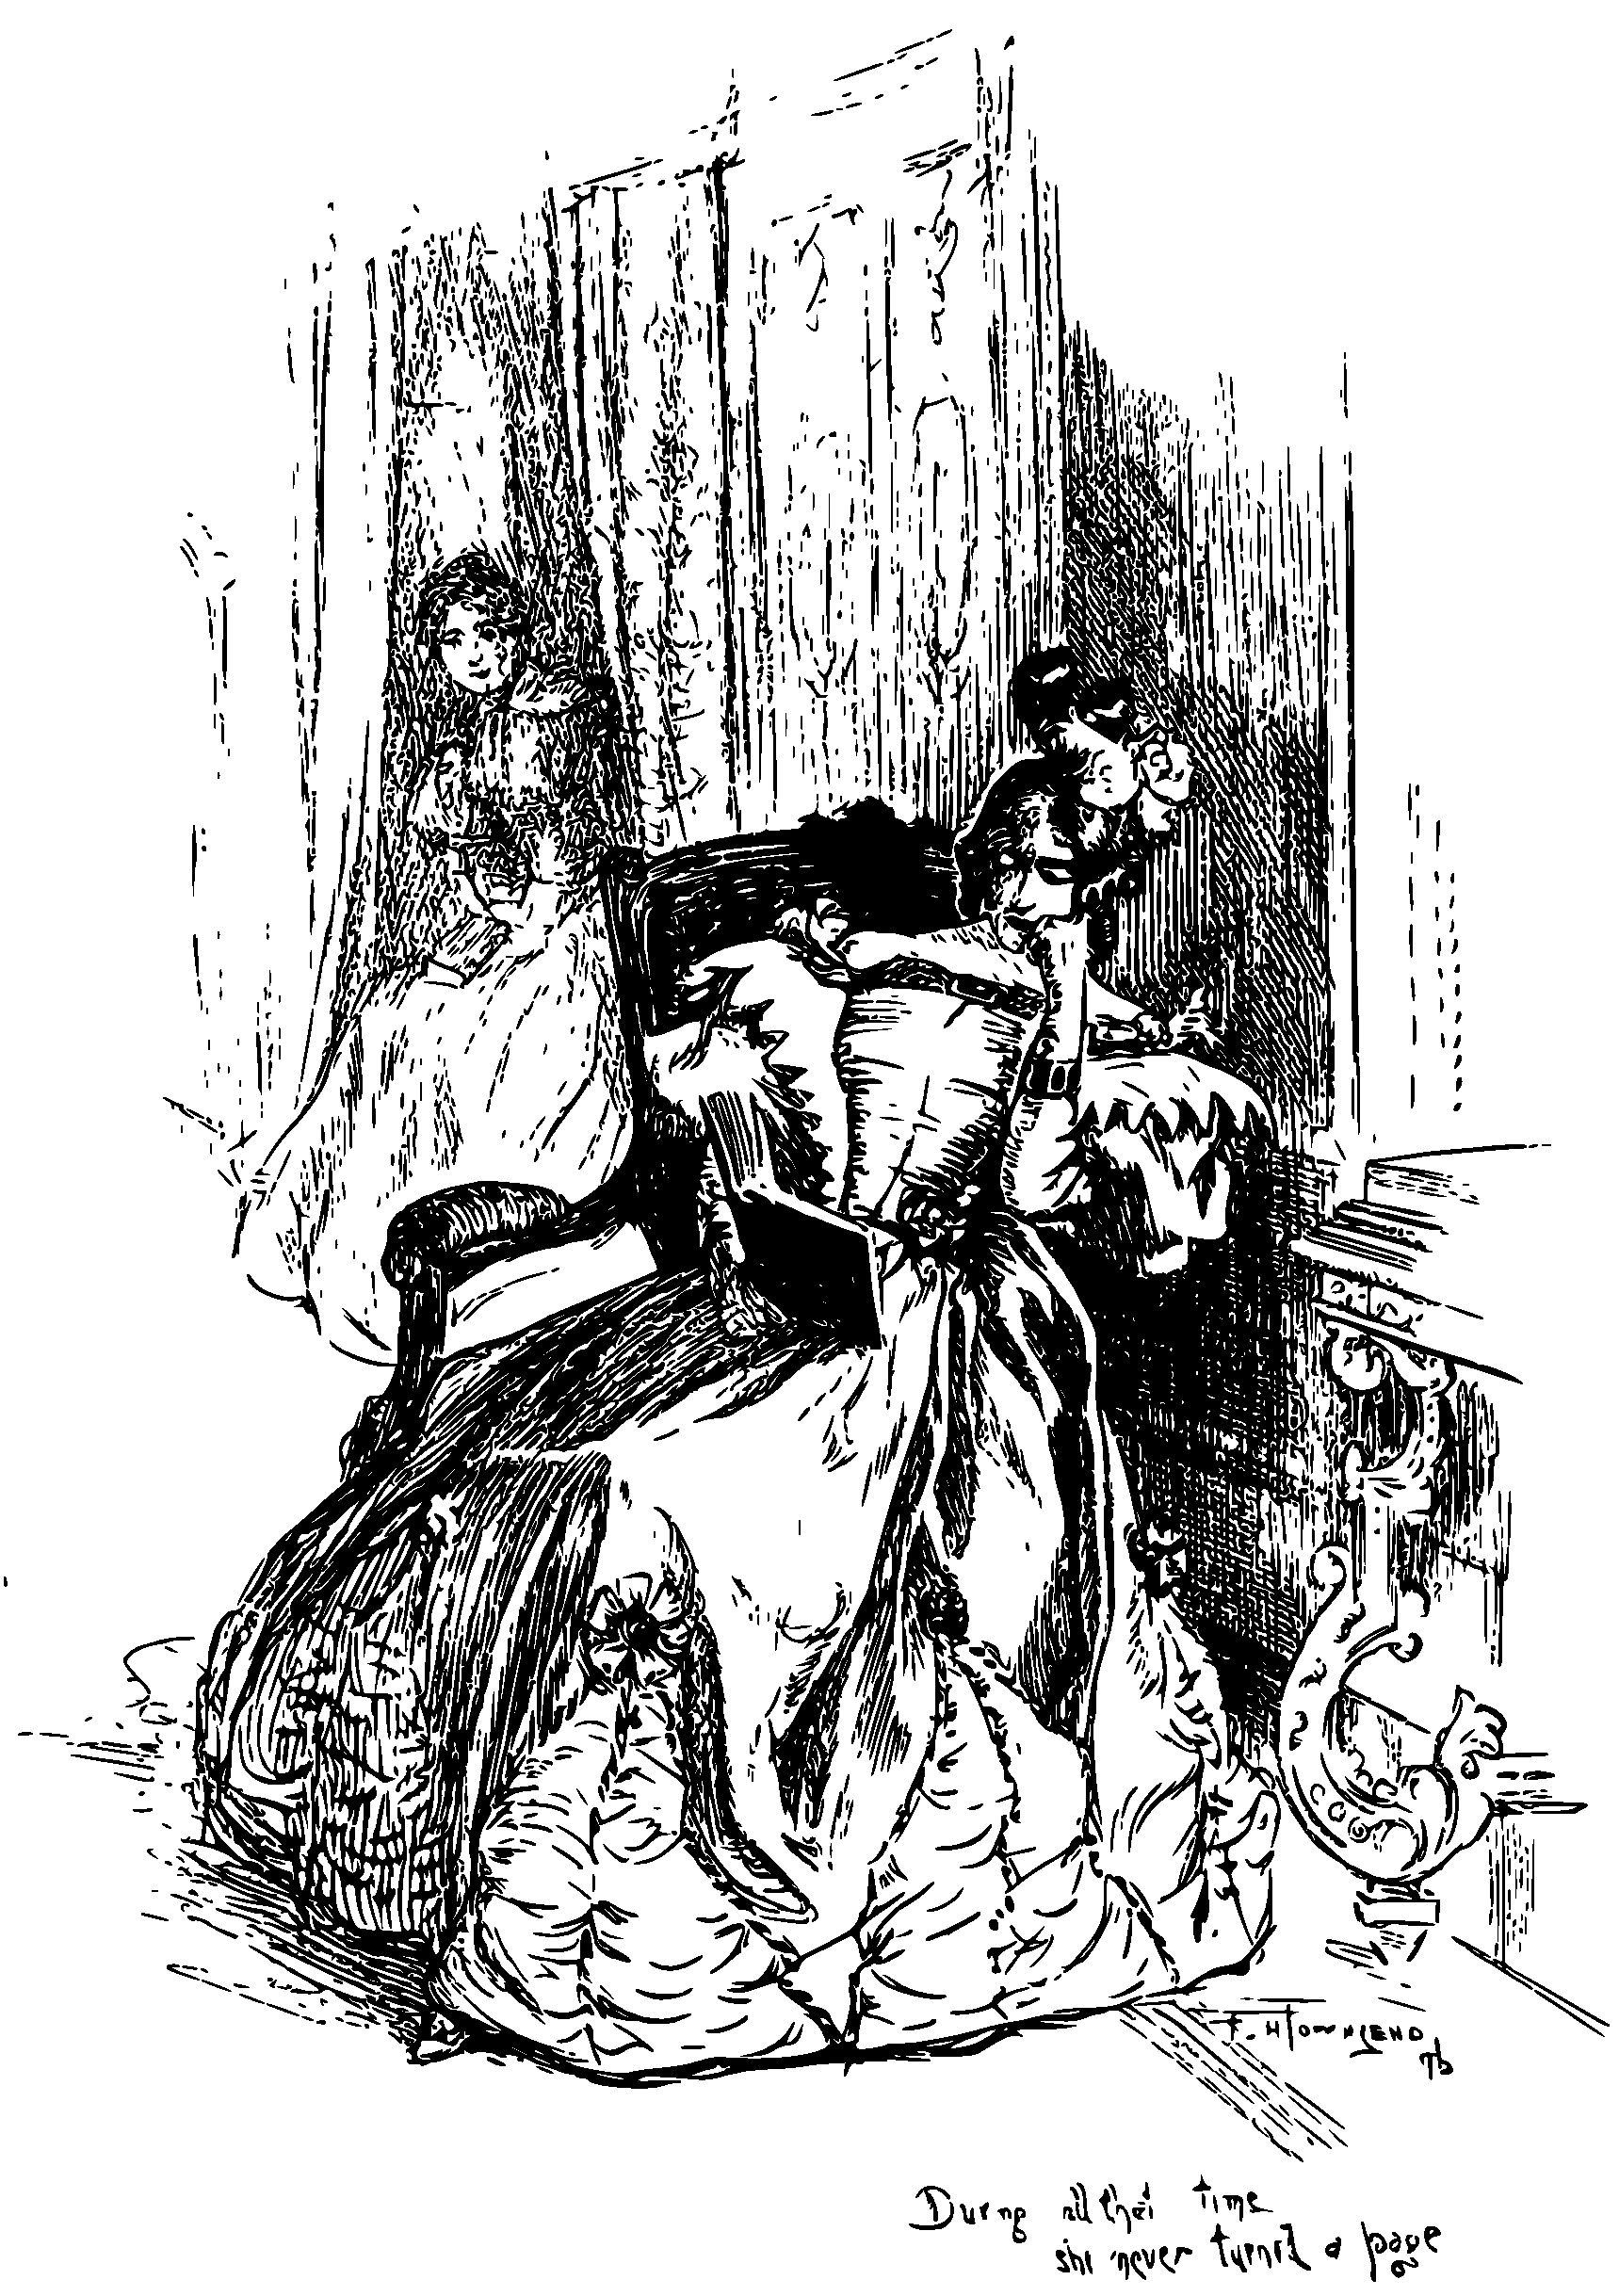
\includegraphics[width=\linewidth]{images/p184b.pdf}
	\end{sidecaption}
\end{figure}

Meantime, Mary Ingram, Amy and Louisa Eshton, declared they dared not go
alone; and yet they all wished to go. A negotiation was opened through
the medium of the ambassador, Sam; and after much pacing to and fro,
till, I think, the said Sam's calves must have ached with the exercise,
permission was at last, with great difficulty, extorted from the
rigorous Sibyl, for the three to wait upon her in a body.

Their visit was not so still as Miss Ingram's had been: we heard
hysterical giggling and little shrieks proceeding from the library; and
at the end of about twenty minutes they burst the door open, and came
running across the hall, as if they were half-scared out of their wits.

\enquote{I am sure she is something not right!} they cried, one and
all. \enquote{She told us such things! She knows all about us!} and
they sank breathless into the various seats the gentlemen hastened to
bring them.

Pressed for further explanation, they declared she had told them of
things they had said and done when they were mere children; described
books and ornaments they had in their boudoirs at home: keepsakes that
different relations had presented to them. They affirmed that she had
even divined their thoughts, and had whispered in the ear of each the
name of the person she liked best in the world, and informed them of
what they most wished for.

Here the gentlemen interposed with earnest petitions to be further
enlightened on these two last-named points; but they got only blushes,
ejaculations, tremors, and titters, in return for their importunity.
The matrons, meantime, offered vinaigrettes and wielded fans; and again
and again reiterated the expression of their concern that their warning
had not been taken in time; and the elder gentlemen laughed, and the
younger urged their services on the agitated fair ones.

In the midst of the tumult, and while my eyes and ears were fully
engaged in the scene before me, I heard a hem close at my elbow: I
turned, and saw Sam.

\enquote{If you please, miss, the gipsy declares that there is another
	young single lady in the room who has not been to her yet, and she
	swears she will not go till she has seen all. I thought it must be you:
	there is no one else for it. What shall I tell her?}

\enquote{Oh, I will go by all means,} I answered: and I was glad of the
unexpected opportunity to gratify my much-excited curiosity. I slipped
out of the room, unobserved by any eye---for the company were gathered
in one mass about the trembling trio just returned---and I closed the
door quietly behind me.

\enquote{If you like, miss,} said Sam, \enquote{I'll wait in the hall
	for you; and if she frightens you, just call and I'll come in.}

\enquote{No, Sam, return to the kitchen: I am not in the least afraid.}
Nor was I; but I was a good deal interested and excited.

\FChapter{Chapter Nineteen}{19}

\Lettrine{T}{he} \textsc{library} looked tranquil enough as I entered it, and the Sibyl---if
Sibyl she were---was seated snugly enough in an easy-chair at the
chimney-corner. She had on a red cloak and a black bonnet: or rather, a
broad-brimmed gipsy hat, tied down with a striped handkerchief under her
chin. An extinguished candle stood on the table; she was bending over
the fire, and seemed reading in a little black book, like a prayer-book,
by the light of the blaze: she muttered the words to herself, as most
old women do, while she read; she did not desist immediately on my
entrance: it appeared she wished to finish a paragraph.

I stood on the rug and warmed my hands, which were rather cold with
sitting at a distance from the drawing-room fire. I felt now as
composed as ever I did in my life: there was nothing indeed in the
gipsy's appearance to trouble one's calm. She shut her book and slowly
looked up; her hat-brim partially shaded her face, yet I could see, as
she raised it, that it was a strange one. It looked all brown and
black: elf-locks bristled out from beneath a white band which passed
under her chin, and came half over her cheeks, or rather jaws: her eye
confronted me at once, with a bold and direct gaze.

\enquote{Well, and you want your fortune told?} she said, in a voice as
decided as her glance, as harsh as her features.

\enquote{I don't care about it, mother; you may please yourself: but I
ought to warn you, I have no faith.}

\enquote{It's like your impudence to say so: I expected it of you; I
heard it in your step as you crossed the threshold.}

\enquote{Did you? You've a quick ear.}

\enquote{I have; and a quick eye and a quick brain.}

\enquote{You need them all in your trade.}

\enquote{I do; especially when I've customers like you to deal with. 
Why don't you tremble?}

\enquote{I'm not cold.}

\enquote{Why don't you turn pale?}

\enquote{I am not sick.}

\enquote{Why don't you consult my art?}

\enquote{I'm not silly.}

The old crone \enquote{nichered} a laugh under her bonnet and bandage;
she then drew out a short black pipe, and lighting it began to smoke. 
Having indulged a while in this sedative, she raised her bent body, took
the pipe from her lips, and while gazing steadily at the fire, said very
deliberately---\enquote{You are cold; you are sick; and you are silly.}

\enquote{Prove it,} I rejoined.

\enquote{I will, in few words. You are cold, because you are alone: no
contact strikes the fire from you that is in you. You are sick; because
the best of feelings, the highest and the sweetest given to man, keeps
far away from you. You are silly, because, suffer as you may, you will
not beckon it to approach, nor will you stir one step to meet it where
it waits you.}

She again put her short black pipe to her lips, and renewed her smoking
with vigour.

\enquote{You might say all that to almost any one who you knew lived as
a solitary dependent in a great house.}

\enquote{I might say it to almost any one: but would it be true of
almost any one?}

\enquote{In my circumstances.}

\enquote{Yes; just so, in \emph{your} circumstances: but find me another
precisely placed as you are.}

\enquote{It would be easy to find you thousands.}

\enquote{You could scarcely find me one. If you knew it, you are
peculiarly situated: very near happiness; yes, within reach of it. The
materials are all prepared; there only wants a movement to combine
them. Chance laid them somewhat apart; let them be once approached and
bliss results.}

\enquote{I don't understand enigmas. I never could guess a riddle in my
life.}

\enquote{If you wish me to speak more plainly, show me your palm.}

\enquote{And I must cross it with silver, I suppose?}

\enquote{To be sure.}

I gave her a shilling: she put it into an old stocking-foot which she
took out of her pocket, and having tied it round and returned it, she
told me to hold out my hand. I did. She approached her face to the
palm, and pored over it without touching it.

\enquote{It is too fine,} said she. \enquote{I can make nothing of such
a hand as that; almost without lines: besides, what is in a palm? 
Destiny is not written there.}

\enquote{I believe you,} said I\@.

\enquote{No,} she continued, \enquote{it is in the face: on the
forehead, about the eyes, in the lines of the mouth. Kneel, and lift up
your head.}

\enquote{Ah! now you are coming to reality,} I said, as I obeyed her. 
\enquote{I shall begin to put some faith in you presently.}

I knelt within half a yard of her. She stirred the fire, so that a
ripple of light broke from the disturbed coal: the glare, however, as
she sat, only threw her face into deeper shadow: mine, it illumined.

\enquote{I wonder with what feelings you came to me to-night,} she said,
when she had examined me a while. \enquote{I wonder what thoughts are
busy in your heart during all the hours you sit in yonder room with the
fine people flitting before you like shapes in a magic-lantern: just as
little sympathetic communion passing between you and them as if they
were really mere shadows of human forms, and not the actual substance.}

\enquote{I feel tired often, sleepy sometimes, but seldom sad.}

\enquote{Then you have some secret hope to buoy you up and please you
with whispers of the future?}

\enquote{Not I\@. The utmost I hope is, to save money enough out of my
earnings to set up a school some day in a little house rented by
myself.}

\enquote{A mean nutriment for the spirit to exist on: and sitting in
that window-seat (you see I know your habits )---}

\enquote{You have learned them from the servants.}

\enquote{Ah! you think yourself sharp. Well, perhaps I have: to speak
truth, I have an acquaintance with one of them, \Mrs{} Poole---}

I started to my feet when I heard the name.

\enquote{You have---have you?} thought I; \enquote{there is diablerie in
the business after all, then!}

\enquote{Don't be alarmed,} continued the strange being; \enquote{she's
a safe hand is \Mrs{} Poole: close and quiet; any one may repose
confidence in her. But, as I was saying: sitting in that window-seat,
do you think of nothing but your future school? Have you no present
interest in any of the company who occupy the sofas and chairs before
you? Is there not one face you study? one figure whose movements you
follow with at least curiosity?}

\enquote{I like to observe all the faces and all the figures.}

\enquote{But do you never single one from the rest---or it may be, two?}

\enquote{I do frequently; when the gestures or looks of a pair seem
telling a tale: it amuses me to watch them.}

\enquote{What tale do you like best to hear?}

\enquote{Oh, I have not much choice! They generally run on the same
theme---courtship; and promise to end in the same
catastrophe---marriage.}

\enquote{And do you like that monotonous theme?}

\enquote{Positively, I don't care about it: it is nothing to me.}

\enquote{Nothing to you? When a lady, young and full of life and
health, charming with beauty and endowed with the gifts of rank and
fortune, sits and smiles in the eyes of a gentleman you---}

\enquote{I what?}

\enquote{You know---and perhaps think well of.}

\enquote{I don't know the gentlemen here. I have scarcely interchanged
a syllable with one of them; and as to thinking well of them, I consider
some respectable, and stately, and middle-aged, and others young,
dashing, handsome, and lively: but certainly they are all at liberty to
be the recipients of whose smiles they please, without my feeling
disposed to consider the transaction of any moment to me.}

\enquote{You don't know the gentlemen here? You have not exchanged a
syllable with one of them? Will you say that of the master of the
house!}

\enquote{He is not at home.}

\enquote{A profound remark! A most ingenious quibble! He went to
Millcote this morning, and will be back here to-night or to-morrow: does
that circumstance exclude him from the list of your acquaintance---blot
him, as it were, out of existence?}

\enquote{No; but I can scarcely see what \Mr{} Rochester has to do with
the theme you had introduced.}

\enquote{I was talking of ladies smiling in the eyes of gentlemen; and
of late so many smiles have been shed into \Mr{} Rochester's eyes that
they overflow like two cups filled above the brim: have you never
remarked that?}

\enquote{\Mr{} Rochester has a right to enjoy the society of his guests.}

\enquote{No question about his right: but have you never observed that,
of all the tales told here about matrimony, \Mr{} Rochester has been
favoured with the most lively and the most continuous?}

\enquote{The eagerness of a listener quickens the tongue of a
narrator.} I said this rather to myself than to the gipsy, whose
strange talk, voice, manner, had by this time wrapped me in a kind of
dream. One unexpected sentence came from her lips after another, till I
got involved in a web of mystification; and wondered what unseen spirit
had been sitting for weeks by my heart watching its workings and taking
record of every pulse.

\enquote{Eagerness of a listener!} repeated she: \enquote{yes; \Mr{}
 Rochester has sat by the hour, his ear inclined to the fascinating lips
that took such delight in their task of communicating; and \Mr{} Rochester
was so willing to receive and looked so grateful for the pastime given
him; you have noticed this?}

\enquote{Grateful! I cannot remember detecting gratitude in his face.}

\enquote{Detecting! You have analysed, then. And what did you detect,
if not gratitude?}

I said nothing.

\enquote{You have seen love: have you not?---and, looking forward, you
have seen him married, and beheld his bride happy?}

\enquote{Humph! Not exactly. Your witch's skill is rather at fault
sometimes.}

\enquote{What the devil have you seen, then?}

\enquote{Never mind: I came here to inquire, not to confess. Is it
known that \Mr{} Rochester is to be married?}

\enquote{Yes; and to the beautiful Miss Ingram.}

\enquote{Shortly?}

\enquote{Appearances would warrant that conclusion: and, no doubt
(though, with an audacity that wants chastising out of you, you seem to
question it), they will be a superlatively happy pair. He must love
such a handsome, noble, witty, accomplished lady; and probably she loves
him, or, if not his person, at least his purse. I know she considers
the Rochester estate eligible to the last degree; though (God pardon
me!) I told her something on that point about an hour ago which made her
look wondrous grave: the corners of her mouth fell half an inch. I
would advise her blackaviced suitor to look out: if another comes, with
a longer or clearer rent-roll,---he's dished---}

\enquote{But, mother, I did not come to hear \Mr{} Rochester's fortune: I
came to hear my own; and you have told me nothing of it.}

\enquote{Your fortune is yet doubtful: when I examined your face, one
trait contradicted another. Chance has meted you a measure of
happiness: that I know. I knew it before I came here this evening. She
has laid it carefully on one side for you. I saw her do it. It depends
on yourself to stretch out your hand, and take it up: but whether you
will do so, is the problem I study. Kneel again on the rug.}

\enquote{Don't keep me long; the fire scorches me.}

\begin{figure}
	\begin{sidecaption}{She did not stoop towards me,\linebreak but only gazed,\linebreak leaning back in her chair.}[p190b]
		\centering
		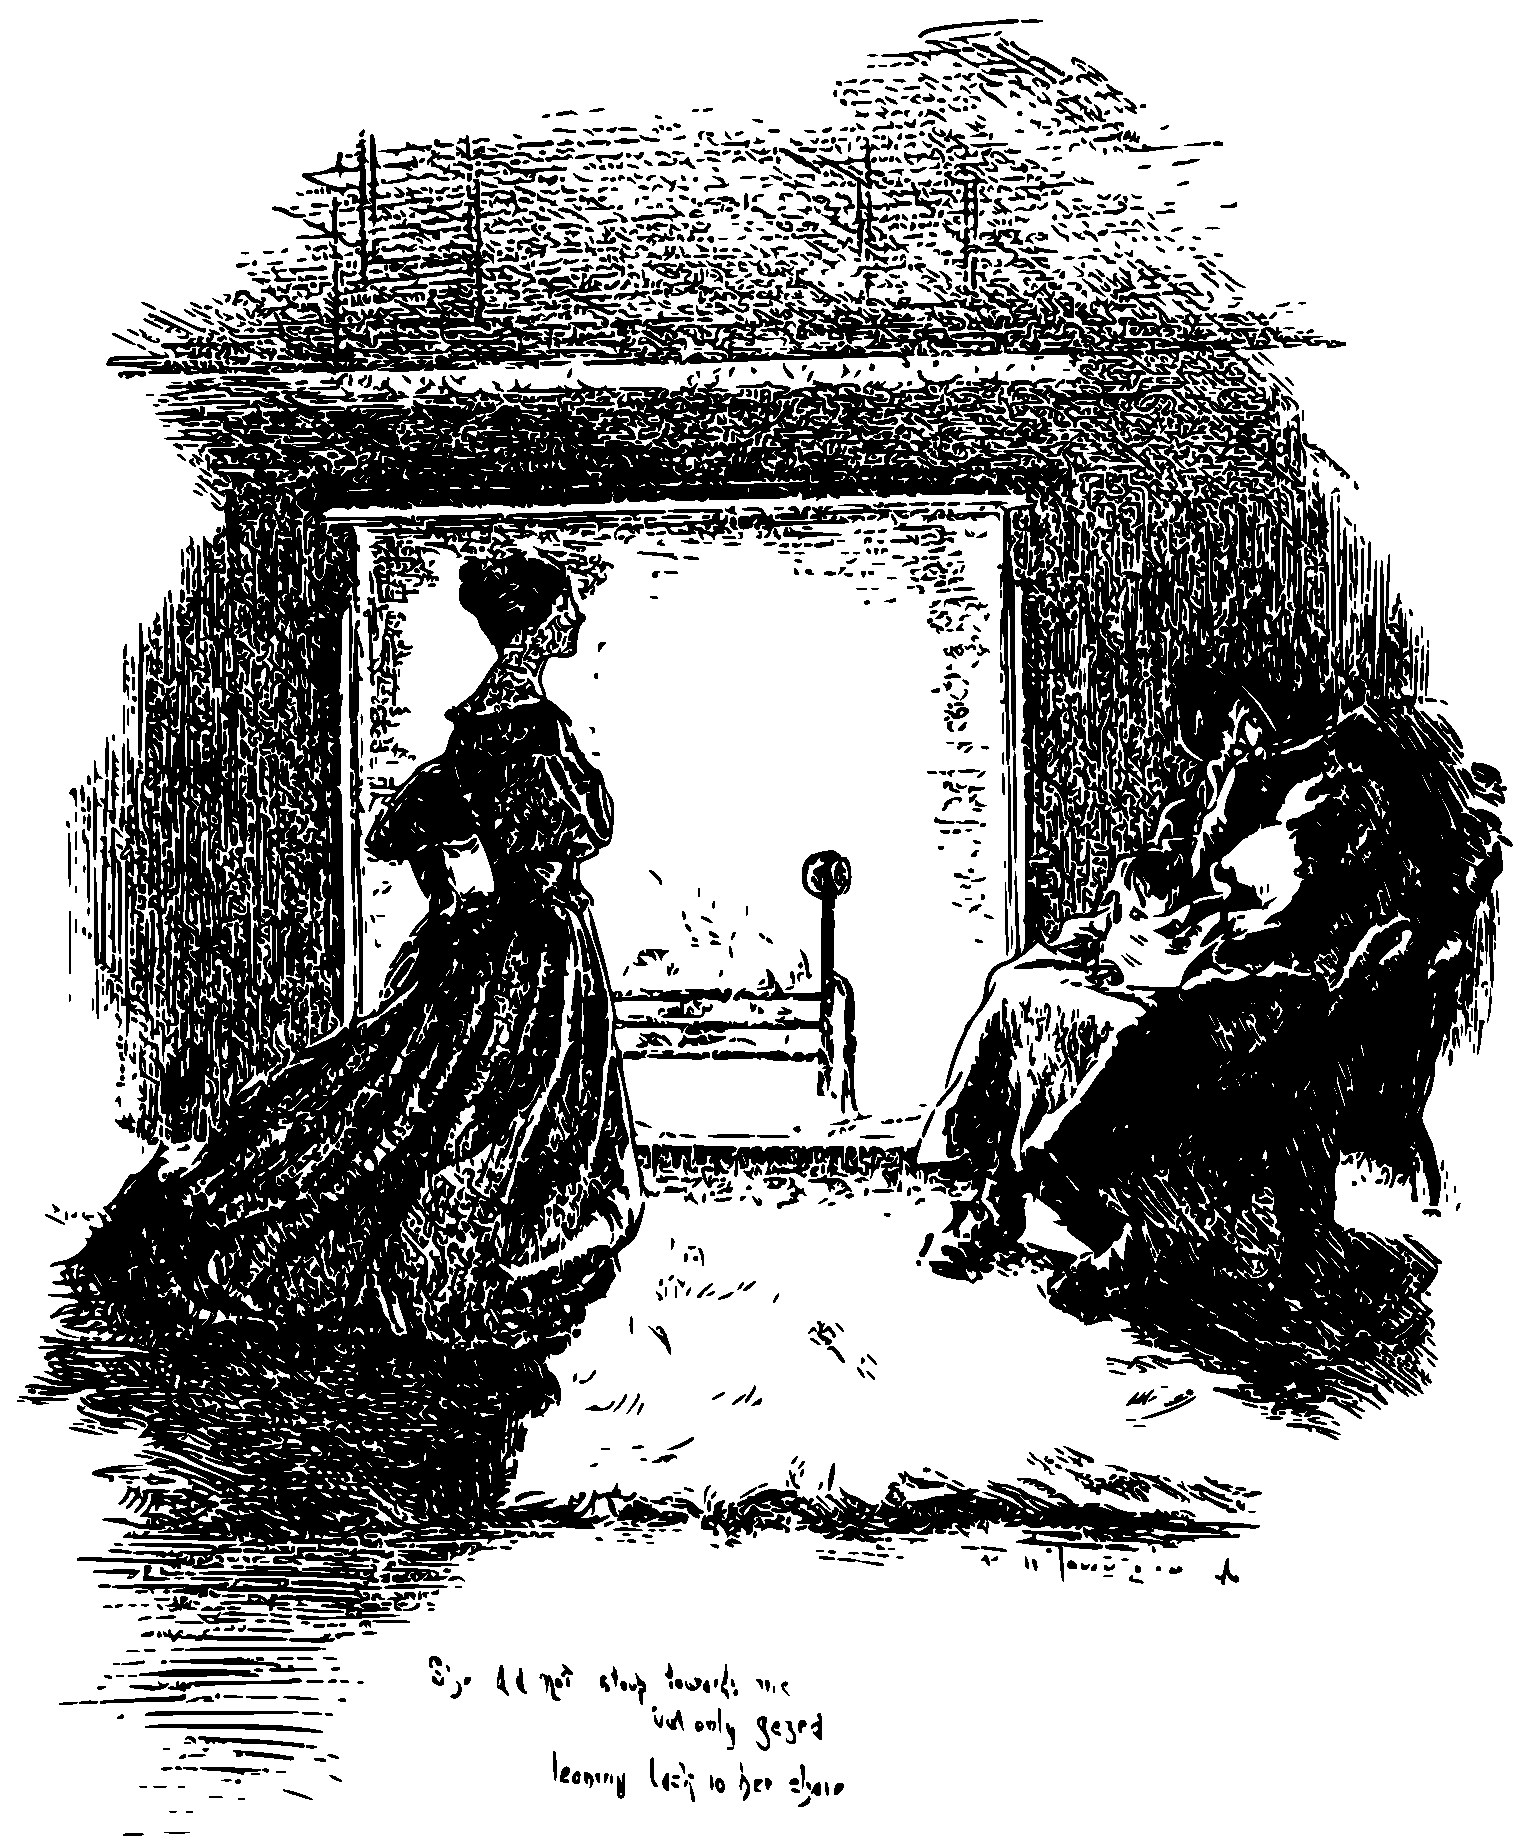
\includegraphics[width=\linewidth]{images/p190b.pdf}
	\end{sidecaption}
\end{figure}

I knelt. She did not stoop towards me, but only gazed, leaning back in
her chair. She began muttering,---

\enquote{The flame flickers in the eye; the eye shines like dew; it looks soft
and full of feeling; it smiles at my jargon: it is susceptible;
impression follows impression through its clear sphere; where it ceases
to smile, it is sad; an unconscious lassitude weighs on the lid: that
signifies melancholy resulting from loneliness. It turns from me; it
will not suffer further scrutiny; it seems to deny, by a mocking glance,
the truth of the discoveries I have already made,---to disown the charge
both of sensibility and chagrin: its pride and reserve only confirm me
in my opinion. The eye is favourable.

%rem enq
As to the mouth, it delights at times in laughter; it is disposed to
impart all that the brain conceives; though I daresay it would be silent
on much the heart experiences. Mobile and flexible, it was never
intended to be compressed in the eternal silence of solitude: it is a
mouth which should speak much and smile often, and have human affection
for its interlocutor. That feature too is propitious.

%rem enq
I see no enemy to a fortunate issue but in the brow; and that brow
professes to say,---\enquote{I can live alone, if self-respect, and
circumstances require me so to do. I need not sell my soul to buy
bliss. I have an inward treasure born with me, which can keep me alive
if all extraneous delights should be withheld, or offered only at a
price I cannot afford to give.} The forehead declares, \enquote{Reason
sits firm and holds the reins, and she will not let the feelings burst
away and hurry her to wild chasms. The passions may rage furiously,
like true heathens, as they are; and the desires may imagine all sorts
of vain things: but judgment shall still have the last word in every
argument, and the casting vote in every decision. Strong wind,
earthquake-shock, and fire may pass by: but I shall follow the guiding
of that still small voice which interprets the dictates of conscience.}

%rem enq
Well said, forehead; your declaration shall be respected. I have
formed my plans---right plans I deem them---and in them I have attended
to the claims of conscience, the counsels of reason. I know how soon
youth would fade and bloom perish, if, in the cup of bliss offered, but
one dreg of shame, or one flavour of remorse were detected; and I do not
want sacrifice, sorrow, dissolution---such is not my taste. I wish to
foster, not to blight---to earn gratitude, not to wring tears of
blood---no, nor of brine: my harvest must be in smiles, in endearments,
in sweet---That will do. I think I rave in a kind of exquisite
delirium. I should wish now to protract this moment \emph{ad
infinitum}; but I dare not. So far I have governed myself thoroughly. 
I have acted as I inwardly swore I would act; but further might try me
beyond my strength. Rise, Miss Eyre: leave me; the play is played
out'.}

Where was I? Did I wake or sleep? Had I been dreaming? Did I dream
still? The old woman's voice had changed: her accent, her gesture, and
all were familiar to me as my own face in a glass---as the speech of my
own tongue. I got up, but did not go. I looked; I stirred the fire,
and I looked again: but she drew her bonnet and her bandage closer about
her face, and again beckoned me to depart. The flame illuminated her
hand stretched out: roused now, and on the alert for discoveries, I at
once noticed that hand. It was no more the withered limb of eld than my
own; it was a rounded supple member, with smooth fingers, symmetrically
turned; a broad ring flashed on the little finger, and stooping forward,
I looked at it, and saw a gem I had seen a hundred times before. Again
I looked at the face; which was no longer turned from me---on the
contrary, the bonnet was doffed, the bandage displaced, the head
advanced.

\enquote{Well, Jane, do you know me?} asked the familiar voice.

\enquote{Only take off the red cloak, sir, and then---}

\enquote{But the string is in a knot---help me.}

\enquote{Break it, sir.}

\enquote{There, then---\enquote{Off, ye lendings!}} And \Mr{} Rochester stepped
out of his disguise.

\enquote{Now, sir, what a strange idea!}

\enquote{But well carried out, eh? Don't you think so?}

\enquote{With the ladies you must have managed well.}

\enquote{But not with you?}

\enquote{You did not act the character of a gipsy with me.}

\enquote{What character did I act? My own?}

\enquote{No; some unaccountable one. In short, I believe you have been
trying to draw me out---or in; you have been talking nonsense to make me
talk nonsense. It is scarcely fair, sir.}

\enquote{Do you forgive me, Jane?}

\enquote{I cannot tell till I have thought it all over. If, on
reflection, I find I have fallen into no great absurdity, I shall try to
forgive you; but it was not right.}

\enquote{Oh, you have been very correct---very careful, very sensible.}

I reflected, and thought, on the whole, I had. It was a comfort; but,
indeed, I had been on my guard almost from the beginning of the
interview. Something of masquerade I suspected. I knew gipsies and
fortune-tellers did not express themselves as this seeming old woman had
expressed herself; besides I had noted her feigned voice, her anxiety to
conceal her features. But my mind had been running on Grace
Poole---that living enigma, that mystery of mysteries, as I considered
her. I had never thought of \Mr{} Rochester.

\enquote{Well,} said he, \enquote{what are you musing about? What does
that grave smile signify?}

\enquote{Wonder and self-congratulation, sir. I have your permission to
retire now, I suppose?}

\enquote{No; stay a moment; and tell me what the people in the
drawing-room yonder are doing.}

\enquote{Discussing the gipsy, I daresay.}

\enquote{Sit down!---Let me hear what they said about me.}

\enquote{I had better not stay long, sir; it must be near eleven
o'clock. Oh, are you aware, \Mr{} Rochester, that a stranger has arrived
here since you left this morning?}

\enquote{A stranger!---no; who can it be? I expected no one; is he
gone?}

\enquote{No; he said he had known you long, and that he could take the
liberty of installing himself here till you returned.}

\enquote{The devil he did! Did he give his name?}

\enquote{His name is Mason, sir; and he comes from the West Indies; from
Spanish Town, in Jamaica, I think.}

\Mr{} Rochester was standing near me; he had taken my hand, as if to lead
me to a chair. As I spoke he gave my wrist a convulsive grip; the smile
on his lips froze: apparently a spasm caught his breath.

\enquote{Mason!---the West Indies!} he said, in the tone one might fancy
a speaking automaton to enounce its single words; \enquote{Mason!---the
West Indies!} he reiterated; and he went over the syllables three times,
growing, in the intervals of speaking, whiter than ashes: he hardly
seemed to know what he was doing.

\enquote{Do you feel ill, sir?} I inquired.

\enquote{Jane, I've got a blow; I've got a blow, Jane!} He staggered.

\enquote{Oh, lean on me, sir.}

\enquote{Jane, you offered me your shoulder once before; let me have it
now.}

\enquote{Yes, sir, yes; and my arm.}

He sat down, and made me sit beside him. Holding my hand in both his
own, he chafed it; gazing on me, at the same time, with the most
troubled and dreary look.

\enquote{My little friend!} said he, \enquote{I wish I were in a quiet
island with only you; and trouble, and danger, and hideous recollections
removed from me.}

\enquote{Can I help you, sir?---I'd give my life to serve you.}

\enquote{Jane, if aid is wanted, I'll seek it at your hands; I promise
you that.}

\enquote{Thank you, sir. Tell me what to do,---I'll try, at least, to
do it.}

\enquote{Fetch me now, Jane, a glass of wine from the dining-room: they
will be at supper there; and tell me if Mason is with them, and what he
is doing.}

I went. I found all the party in the dining-room at supper, as \Mr{}
 Rochester had said; they were not seated at table,---the supper was
arranged on the sideboard; each had taken what he chose, and they stood
about here and there in groups, their plates and glasses in their
hands. Every one seemed in high glee; laughter and conversation were
general and animated. \Mr{} Mason stood near the fire, talking to Colonel
and \Mrs{} Dent, and appeared as merry as any of them. I filled a
wine-glass (I saw Miss Ingram watch me frowningly as I did so: she
thought I was taking a liberty, I daresay), and I returned to the
library.

\Mr{} Rochester's extreme pallor had disappeared, and he looked once more
firm and stern. He took the glass from my hand.

\enquote{Here is to your health, ministrant spirit!} he said. He
swallowed the contents and returned it to me. \enquote{What are they
doing, Jane?}

\enquote{Laughing and talking, sir.}

\enquote{They don't look grave and mysterious, as if they had heard
something strange?}

\enquote{Not at all: they are full of jests and gaiety.}

\enquote{And Mason?}

\enquote{He was laughing too.}

\enquote{If all these people came in a body and spat at me, what would
you do, Jane?}

\enquote{Turn them out of the room, sir, if I could.}

He half smiled. \enquote{But if I were to go to them, and they only
looked at me coldly, and whispered sneeringly amongst each other, and
then dropped off and left me one by one, what then? Would you go with
them?}

\enquote{I rather think not, sir: I should have more pleasure in staying
with you.}

\enquote{To comfort me?}

\enquote{Yes, sir, to comfort you, as well as I could.}

\enquote{And if they laid you under a ban for adhering to me?}

\enquote{I, probably, should know nothing about their ban; and if I did,
I should care nothing about it.}

\enquote{Then, you could dare censure for my sake?}

\enquote{I could dare it for the sake of any friend who deserved my
adherence; as you, I am sure, do.}

\enquote{Go back now into the room; step quietly up to Mason, and
whisper in his ear that \Mr{} Rochester is come and wishes to see him:
show him in here and then leave me.}

\enquote{Yes, sir.}

I did his behest. The company all stared at me as I passed straight
among them. I sought \Mr{} Mason, delivered the message, and preceded him
from the room: I ushered him into the library, and then I went upstairs.

At a late hour, after I had been in bed some time, I heard the visitors
repair to their chambers: I distinguished \Mr{} Rochester's voice, and
heard him say, \enquote{This way, Mason; this is your room.}

He spoke cheerfully: the gay tones set my heart at ease. I was soon
asleep.

\FChapter{Chapter Twenty}{20}

\Lettrine{I}{} \textsc{had forgotten} to draw my curtain, which I usually did, and also to let
down my window-blind. The consequence was, that when the moon, which
was full and bright (for the night was fine), came in her course to that
space in the sky opposite my casement, and looked in at me through the
unveiled panes, her glorious gaze roused me. Awaking in the dead of
night, I opened my eyes on her disk---silver-white and crystal clear.
It was beautiful, but too solemn; I half rose, and stretched my arm to
draw the curtain.

Good God! What a cry!

The night---its silence---its rest, was rent in twain by a savage, a
sharp, a shrilly sound that ran from end to end of Thornfield Hall.

My pulse stopped: my heart stood still; my stretched arm was paralysed.
The cry died, and was not renewed. Indeed, whatever being uttered that
fearful shriek could not soon repeat it: not the widest-winged condor on
the Andes could, twice in succession, send out such a yell from the
cloud shrouding his eyrie. The thing delivering such utterance must
rest ere it could repeat the effort.

It came out of the third storey; for it passed overhead. And
overhead---yes, in the room just above my chamber-ceiling---I now heard
a struggle: a deadly one it seemed from the noise; and a half-smothered
voice shouted---

\enquote{Help! help! help!} three times rapidly.

\enquote{Will no one come?} it cried; and then, while the staggering and
stamping went on wildly, I distinguished through plank and plaster:---

\enquote{ Rochester!Rochester! for God's sake, come!}

A chamber-door opened: some one ran, or rushed, along the gallery.
Another step stamped on the flooring above and something fell; and there
was silence.

I had put on some clothes, though horror shook all my limbs; I issued
from my apartment. The sleepers were all aroused: ejaculations,
terrified murmurs sounded in every room; door after door unclosed; one
looked out and another looked out; the gallery filled. Gentlemen and
ladies alike had quitted their beds; and \enquote{Oh! what is
	it?}---\enquote{Who is hurt?}---\enquote{What has
	happened?}---\enquote{Fetch a light!}---\enquote{Is it
	fire?}---\enquote{Are there robbers?}---\enquote{Where shall we run?}
was demanded confusedly on all hands. But for the moonlight they would
have been in complete darkness. They ran to and fro; they crowded
together: some sobbed, some stumbled: the confusion was inextricable.

\enquote{Where the devil is Rochester?} cried Colonel Dent. \enquote{I
	cannot find him in his bed.}

\enquote{Here! here!} was shouted in return. \enquote{Be composed, all
	of you: I'm coming.}

And the door at the end of the gallery opened, and \Mr{} Rochester
advanced with a candle: he had just descended from the upper storey.
One of the ladies ran to him directly; she seized his arm: it was Miss
Ingram.

\enquote{What awful event has taken place?} said she. \enquote{Speak!
	let us know the worst at once!}

\enquote{But don't pull me down or strangle me,} he replied: for the
Misses Eshton were clinging about him now; and the two dowagers, in vast
white wrappers, were bearing down on him like ships in full sail.

\enquote{All's right!---all's right!} he cried. \enquote{It's a mere
	rehearsal of Much Ado about Nothing. Ladies, keep off, or I shall wax
	dangerous.}

And dangerous he looked: his black eyes darted sparks. Calming himself
by an effort, he added---

\enquote{A servant has had the nightmare; that is all. She's an
	excitable, nervous person: she construed her dream into an apparition,
	or something of that sort, no doubt; and has taken a fit with fright.
	Now, then, I must see you all back into your rooms; for, till the house
	is settled, she cannot be looked after. Gentlemen, have the goodness to
	set the ladies the example. Miss Ingram, I am sure you will not fail in
	evincing superiority to idle terrors. Amy and Louisa, return to your
	nests like a pair of doves, as you are.  Mesdames} (to the dowagers),
\enquote{you will take cold to a dead certainty, if you stay in this
	chill gallery any longer.}

And so, by dint of alternate coaxing and commanding, he contrived to get
them all once more enclosed in their separate dormitories. I did not
wait to be ordered back to mine, but retreated unnoticed, as unnoticed I
had left it.

Not, however, to go to bed: on the contrary, I began and dressed myself
carefully. The sounds I had heard after the scream, and the words that
had been uttered, had probably been heard only by me; for they had
proceeded from the room above mine: but they assured me that it was not
a servant's dream which had thus struck horror through the house; and
that the explanation \Mr{} Rochester had given was merely an invention
framed to pacify his guests. I dressed, then, to be ready for
emergencies. When dressed, I sat a long time by the window looking out
over the silent grounds and silvered fields and waiting for I knew not
what. It seemed to me that some event must follow the strange cry,
struggle, and call.

No: stillness returned: each murmur and movement ceased gradually, and
in about an hour Thornfield Hall was again as hushed as a desert. It
seemed that sleep and night had resumed their empire. Meantime the moon
declined: she was about to set. Not liking to sit in the cold and
darkness, I thought I would lie down on my bed, dressed as I was. I
left the window, and moved with little noise across the carpet; as I
stooped to take off my shoes, a cautious hand tapped low at the door.

\enquote{Am I wanted?} I asked.

\enquote{Are you up?} asked the voice I expected to hear, viz., my
master's.

\enquote{Yes, sir.}

\enquote{And dressed?}

\enquote{Yes.}

\enquote{Come out, then, quietly.}

I obeyed. \Mr{} Rochester stood in the gallery holding a light.

\enquote{I want you,} he said: \enquote{come this way: take your time,
	and make no noise.}

My slippers were thin: I could walk the matted floor as softly as a
cat. He glided up the gallery and up the stairs, and stopped in the
dark, low corridor of the fateful third storey: I had followed and stood
at his side.

\enquote{Have you a sponge in your room?} he asked in a whisper.

\enquote{Yes, sir.}

\enquote{Have you any salts---volatile salts?}

\enquote{Yes.}

\enquote{Go back and fetch both.}

I returned, sought the sponge on the washstand, the salts in my drawer,
and once more retraced my steps. He still waited; he held a key in his
hand: approaching one of the small, black doors, he put it in the lock;
he paused, and addressed me again.

\enquote{You don't turn sick at the sight of blood?}

\enquote{I think I shall not: I have never been tried yet.}

I felt a thrill while I answered him; but no coldness, and no faintness.

\enquote{Just give me your hand,} he said: \enquote{it will not do to
	risk a fainting fit.}

I put my fingers into his. \enquote{Warm and steady,} was his remark:
he turned the key and opened the door.

I saw a room I remembered to have seen before, the day \Mrs{} Fairfax
showed me over the house: it was hung with tapestry; but the tapestry
was now looped up in one part, and there was a door apparent, which had
then been concealed. This door was open; a light shone out of the room
within: I heard thence a snarling, snatching sound, almost like a dog
quarrelling. \Mr{} Rochester, putting down his candle, said to me,
\enquote{Wait a minute,} and he went forward to the inner apartment. A
shout of laughter greeted his entrance; noisy at first, and terminating
in Grace Poole's own goblin ha! ha! \emph{She} then was there. He made
some sort of arrangement without speaking, though I heard a low voice
address him: he came out and closed the door behind him.

\enquote{Here, Jane!} he said; and I walked round to the other side of a
large bed, which with its drawn curtains concealed a considerable
portion of the chamber. An easy-chair was near the bed-head: a man sat
in it, dressed with the exception of his coat; he was still; his head
leant back; his eyes were closed. \Mr{} Rochester held the candle over
him; I recognised in his pale and seemingly lifeless face---the
stranger, Mason: I saw too that his linen on one side, and one arm, was
almost soaked in blood.

\enquote{Hold the candle,} said \Mr{} Rochester, and I took it: he fetched
a basin of water from the washstand: \enquote{Hold that,} said he. I
obeyed. He took the sponge, dipped it in, and moistened the corpse-like
face; he asked for my smelling-bottle, and applied it to the nostrils.
\Mr{} Mason shortly unclosed his eyes; he groaned. \Mr{} Rochester opened
the shirt of the wounded man, whose arm and shoulder were bandaged: he
sponged away blood, trickling fast down.

\enquote{Is there immediate danger?} murmured \Mr{} Mason.

\enquote{Pooh! No---a mere scratch. Don't be so overcome, man: bear
	up! I'll fetch a surgeon for you now, myself: you'll be able to be
	removed by morning, I hope. Jane,} he continued.

\enquote{Sir?}

\enquote{I shall have to leave you in this room with this gentleman, for
	an hour, or perhaps two hours: you will sponge the blood as I do when it
	returns: if he feels faint, you will put the glass of water on that
	stand to his lips, and your salts to his nose. You will not speak to
	him on any pretext---and---Richard, it will be at the peril of your life
	if you speak to her: open your lips---agitate yourself---and I'll not
	answer for the consequences.}

Again the poor man groaned; he looked as if he dared not move; fear,
either of death or of something else, appeared almost to paralyse him.
\Mr{} Rochester put the now bloody sponge into my hand, and I proceeded to
use it as he had done. He watched me a second, then saying,
\enquote{Remember!---No conversation,} he left the room. I experienced
a strange feeling as the key grated in the lock, and the sound of his
retreating step ceased to be heard.

Here then I was in the third storey, fastened into one of its mystic
cells; night around me; a pale and bloody spectacle under my eyes and
hands; a murderess hardly separated from me by a single door: yes---that
was appalling---the rest I could bear; but I shuddered at the thought of
Grace Poole bursting out upon me.

I must keep to my post, however. I must watch this ghastly
countenance---these blue, still lips forbidden to unclose---these eyes
now shut, now opening, now wandering through the room, now fixing on me,
and ever glazed with the dulness of horror. I must dip my hand again
and again in the basin of blood and water, and wipe away the trickling
gore. I must see the light of the unsnuffed candle wane on my
employment; the shadows darken on the wrought, antique tapestry round
me, and grow black under the hangings of the vast old bed, and quiver
strangely over the doors of a great cabinet opposite---whose front,
divided into twelve panels, bore, in grim design, the heads of the
twelve apostles, each enclosed in its separate panel as in a frame;
while above them at the top rose an ebon crucifix and a dying Christ.

According as the shifting obscurity and flickering gleam hovered here or
glanced there, it was now the bearded physician, Luke, that bent his
brow; now \St{} John's long hair that waved; and anon the devilish face of
Judas, that grew out of the panel, and seemed gathering life and
threatening a revelation of the arch-traitor---of Satan himself---in his
subordinate's form.

Amidst all this, I had to listen as well as watch: to listen for the
movements of the wild beast or the fiend in yonder side den. But since
\Mr{} Rochester's visit it seemed spellbound: all the night I heard but
three sounds at three long intervals,---a step creak, a momentary
renewal of the snarling, canine noise, and a deep human groan.

Then my own thoughts worried me. What crime was this that lived
incarnate in this sequestered mansion, and could neither be expelled nor
subdued by the owner?---what mystery, that broke out now in fire and now
in blood, at the deadest hours of night? What creature was it, that,
masked in an ordinary woman's face and shape, uttered the voice, now of
a mocking demon, and anon of a carrion-seeking bird of prey?

And this man I bent over---this commonplace, quiet stranger---how had he
become involved in the web of horror? and why had the Fury flown at
him? What made him seek this quarter of the house at an untimely
season, when he should have been asleep in bed? I had heard \Mr{}
Rochester assign him an apartment below---what brought him here! And
why, now, was he so tame under the violence or treachery done him? Why
did he so quietly submit to the concealment \Mr{} Rochester enforced? Why
\emph{did} \Mr{} Rochester enforce this concealment? His guest had been
outraged, his own life on a former occasion had been hideously plotted
against; and both attempts he smothered in secrecy and sank in
oblivion! Lastly, I saw \Mr{} Mason was submissive to \Mr{} Rochester; that
the impetuous will of the latter held complete sway over the inertness
of the former: the few words which had passed between them assured me of
this. It was evident that in their former intercourse, the passive
disposition of the one had been habitually influenced by the active
energy of the other: whence then had arisen \Mr{} Rochester's dismay when
he heard of \Mr{} Mason's arrival? Why had the mere name of this
unresisting individual---whom his word now sufficed to control like a
child---fallen on him, a few hours since, as a thunderbolt might fall on
an oak?

Oh! I could not forget his look and his paleness when he whispered:
\enquote{Jane, I have got a blow---I have got a blow, Jane.} I could
not forget how the arm had trembled which he rested on my shoulder: and
it was no light matter which could thus bow the resolute spirit and
thrill the vigorous frame of Fairfax Rochester.

\enquote{When will he come? When will he come?} I cried inwardly, as
the night lingered and lingered---as my bleeding patient drooped,
moaned, sickened: and neither day nor aid arrived. I had, again and
again, held the water to Mason's white lips; again and again offered him
the stimulating salts: my efforts seemed ineffectual: either bodily or
mental suffering, or loss of blood, or all three combined, were fast
prostrating his strength. He moaned so, and looked so weak, wild, and
lost, I feared he was dying; and I might not even speak to him.

The candle, wasted at last, went out; as it expired, I perceived streaks
of grey light edging the window curtains: dawn was then approaching.
Presently I heard Pilot bark far below, out of his distant kennel in the
courtyard: hope revived. Nor was it unwarranted: in five minutes more
the grating key, the yielding lock, warned me my watch was relieved. It
could not have lasted more than two hours: many a week has seemed
shorter.

\Mr{} Rochester entered, and with him the surgeon he had been to fetch.

\enquote{Now, Carter, be on the alert,} he said to this last: \enquote{I
	give you but half-an-hour for dressing the wound, fastening the
	bandages, getting the patient downstairs and all.}

\enquote{But is he fit to move, sir?}

\enquote{No doubt of it; it is nothing serious; he is nervous, his
	spirits must be kept up. Come, set to work.}

\Mr{} Rochester drew back the thick curtain, drew up the holland blind,
let in all the daylight he could; and I was surprised and cheered to see
how far dawn was advanced: what rosy streaks were beginning to brighten
the east. Then he approached Mason, whom the surgeon was already
handling.

\enquote{Now, my good fellow, how are you?} he asked.

\enquote{She's done for me, I fear,} was the faint reply.

\enquote{Not a whit!---courage! This day fortnight you'll hardly be a
	pin the worse of it: you've lost a little blood; that's all. Carter,
	assure him there's no danger.}

\enquote{I can do that conscientiously,} said Carter, who had now undone
the bandages; \enquote{only I wish I could have got here sooner: he
	would not have bled so much---but how is this? The flesh on the
	shoulder is torn as well as cut. This wound was not done with a knife:
	there have been teeth here!}

\enquote{She bit me,} he murmured. \enquote{She worried me like a
	tigress, when Rochester got the knife from her.}

\enquote{You should not have yielded: you should have grappled with her
	at once,} said \Mr{} Rochester.

\enquote{But under such circumstances, what could one do?} returned
Mason. \enquote{Oh, it was frightful!} he added, shuddering.
\enquote{And I did not expect it: she looked so quiet at first.}

\enquote{I warned you,} was his friend's answer; \enquote{I said---be on
	your guard when you go near her. Besides, you might have waited till
	to-morrow, and had me with you: it was mere folly to attempt the
	interview to-night, and alone.}

\enquote{I thought I could have done some good.}

\enquote{You thought! you thought! Yes, it makes me impatient to hear
	you: but, however, you have suffered, and are likely to suffer enough
	for not taking my advice; so I'll say no more.
	Carter---hurry!---hurry! The sun will soon rise, and I must have him
	off.}

\enquote{Directly, sir; the shoulder is just bandaged. I must look to
	this other wound in the arm: she has had her teeth here too, I think.}

\enquote{She sucked the blood: she said she'd drain my heart,} said
Mason.

I saw \Mr{} Rochester shudder: a singularly marked expression of disgust,
horror, hatred, warped his countenance almost to distortion; but he only
said---

\enquote{Come, be silent, Richard, and never mind her gibberish: don't
	repeat it.}

\enquote{I wish I could forget it,} was the answer.

\enquote{You will when you are out of the country: when you get back to
	Spanish Town, you may think of her as dead and buried---or rather, you
	need not think of her at all.}

\enquote{Impossible to forget this night!}

\enquote{It is not impossible: have some energy, man. You thought you
	were as dead as a herring two hours since, and you are all alive and
	talking now. There!---Carter has done with you or nearly so; I'll make
	you decent in a trice. Jane} (he turned to me for the first time since
his re-entrance), \enquote{take this key: go down into my bedroom, and
	walk straight forward into my dressing-room: open the top drawer of the
	wardrobe and take out a clean shirt and neck-handkerchief: bring them
	here; and be nimble.}

I went; sought the repository he had mentioned, found the articles
named, and returned with them.

\enquote{Now,} said he, \enquote{go to the other side of the bed while I
	order his toilet; but don't leave the room: you may be wanted again.}

I retired as directed.

\enquote{Was anybody stirring below when you went down, Jane?} inquired
\Mr{} Rochester presently.

\enquote{No, sir; all was very still.}

\enquote{We shall get you off cannily, Dick: and it will be better, both
	for your sake, and for that of the poor creature in yonder. I have
	striven long to avoid exposure, and I should not like it to come at
	last. Here, Carter, help him on with his waist-coat. Where did you
	leave your furred cloak? You can't travel a mile without that, I know,
	in this damned cold climate. In your room?---Jane, run down to \Mr{}
	Mason's room,---the one next mine,---and fetch a cloak you will see
	there.}

Again I ran, and again returned, bearing an immense mantle lined and
edged with fur.

\enquote{Now, I've another errand for you,} said my untiring master;
\enquote{you must away to my room again. What a mercy you are shod with
	velvet, Jane!---a clod-hopping messenger would never do at this
	juncture. You must open the middle drawer of my toilet-table and take
	out a little phial and a little glass you will find there,---quick!}

I flew thither and back, bringing the desired vessels.

\enquote{That's well! Now, doctor, I shall take the liberty of
	administering a dose myself, on my own responsibility. I got this
	cordial at Rome, of an Italian charlatan---a fellow you would have
	kicked, Carter. It is not a thing to be used indiscriminately, but it
	is good upon occasion: as now, for instance. Jane, a little water.}

He held out the tiny glass, and I half filled it from the water-bottle
on the washstand.

\enquote{That will do;---now wet the lip of the phial.}

I did so; he measured twelve drops of a crimson liquid, and presented it
to Mason.

\enquote{Drink, Richard: it will give you the heart you lack, for an
	hour or so.}

\enquote{But will it hurt me?---is it inflammatory?}

\enquote{Drink! drink! drink!}

\Mr{} Mason obeyed, because it was evidently useless to resist. He was
dressed now: he still looked pale, but he was no longer gory and
sullied. \Mr{} Rochester let him sit three minutes after he had swallowed
the liquid; he then took his arm---

\enquote{Now I am sure you can get on your feet,} he
said---\enquote{try.}

The patient rose.

\enquote{Carter, take him under the other shoulder. Be of good cheer,
	Richard; step out---that's it!}

\enquote{I do feel better,} remarked \Mr{} Mason.

\enquote{I am sure you do. Now, Jane, trip on before us away to the
	backstairs; unbolt the side-passage door, and tell the driver of the
	post-chaise you will see in the yard---or just outside, for I told him
	not to drive his rattling wheels over the pavement---to be ready; we are
	coming: and, Jane, if any one is about, come to the foot of the stairs
	and hem.}

It was by this time half-past five, and the sun was on the point of
rising; but I found the kitchen still dark and silent. The side-passage
door was fastened; I opened it with as little noise as possible: all the
yard was quiet; but the gates stood wide open, and there was a
post-chaise, with horses ready harnessed, and driver seated on the box,
stationed outside. I approached him, and said the gentlemen were
coming; he nodded: then I looked carefully round and listened. The
stillness of early morning slumbered everywhere; the curtains were yet
drawn over the servants' chamber windows; little birds were just
twittering in the blossom-blanched orchard trees, whose boughs drooped
like white garlands over the wall enclosing one side of the yard; the
carriage horses stamped from time to time in their closed stables: all
else was still.

The gentlemen now appeared. Mason, supported by \Mr{} Rochester and the
surgeon, seemed to walk with tolerable ease: they assisted him into the
chaise; Carter followed.

\enquote{Take care of him,} said \Mr{} Rochester to the latter,
\enquote{and keep him at your house till he is quite well: I shall ride
	over in a day or two to see how he gets on. Richard, how is it with
	you?}

\enquote{The fresh air revives me, Fairfax.}

\enquote{Leave the window open on his side, Carter; there is no
	wind---good-bye, Dick.}

\enquote{Fairfax---}

\enquote{Well what is it?}

\enquote{Let her be taken care of; let her be treated as tenderly as may
	be: let her---} he stopped and burst into tears.

\enquote{I do my best; and have done it, and will do it,} was the
answer: he shut up the chaise door, and the vehicle drove away.

\enquote{Yet would to God there was an end of all this!} added \Mr{}
Rochester, as he closed and barred the heavy yard-gates.

This done, he moved with slow step and abstracted air towards a door in
the wall bordering the orchard. I, supposing he had done with me,
prepared to return to the house; again, however, I heard him call
\enquote{Jane!} He had opened the portal and stood at it, waiting for
me.

\enquote{Come where there is some freshness, for a few moments,} he
said; \enquote{that house is a mere dungeon: don't you feel it so?}

\enquote{It seems to me a splendid mansion, sir.}

\enquote{The glamour of inexperience is over your eyes,} he answered;
\enquote{and you see it through a charmed medium: you cannot discern that the
	gilding is slime and the silk draperies cobwebs; that the marble is
	sordid slate, and the polished woods mere refuse chips and scaly bark.
	Now \emph{here}} (he pointed to the leafy enclosure we had entered)
\enquote{all is real, sweet, and pure.}

He strayed down a walk edged with box, with apple trees, pear trees, and
cherry trees on one side, and a border on the other full of all sorts of
old-fashioned flowers, stocks, sweet-williams, primroses, pansies,
mingled with southernwood, sweet-briar, and various fragrant herbs.
They were fresh now as a succession of April showers and gleams,
followed by a lovely spring morning, could make them: the sun was just
entering the dappled east, and his light illumined the wreathed and dewy
orchard trees and shone down the quiet walks under them.

\enquote{Jane, will you have a flower?}

He gathered a half-blown rose, the first on the bush, and offered it to
me.

\enquote{Thank you, sir.}

\enquote{Do you like this sunrise, Jane? That sky with its high and
	light clouds which are sure to melt away as the day waxes warm---this
	placid and balmly atmosphere?}

\enquote{I do, very much.}

\enquote{You have passed a strange night, Jane.}

\enquote{Yes, sir.}

\enquote{And it has made you look pale---were you afraid when I left you
	alone with Mason?}

\enquote{I was afraid of some one coming out of the inner room.}

\enquote{But I had fastened the door---I had the key in my pocket: I
	should have been a careless shepherd if I had left a lamb---my pet
	lamb---so near a wolf's den, unguarded: you were safe.}

\enquote{Will Grace Poole live here still, sir?}

\enquote{Oh yes! don't trouble your head about her---put the thing out
	of your thoughts.}

\enquote{Yet it seems to me your life is hardly secure while she stays.}

\enquote{Never fear---I will take care of myself.}

\enquote{Is the danger you apprehended last night gone by now, sir?}

\enquote{I cannot vouch for that till Mason is out of England: nor even
	then. To live, for me, Jane, is to stand on a crater-crust which may
	crack and spue fire any day.}

\enquote{But \Mr{} Mason seems a man easily led. Your influence, sir, is
	evidently potent with him: he will never set you at defiance or wilfully
	injure you.}

\enquote{Oh, no! Mason will not defy me; nor, knowing it, will he hurt
	me---but, unintentionally, he might in a moment, by one careless word,
	deprive me, if not of life, yet for ever of happiness.}

\enquote{Tell him to be cautious, sir: let him know what you fear, and
	show him how to avert the danger.}

He laughed sardonically, hastily took my hand, and as hastily threw it
from him.

\enquote{If I could do that, simpleton, where would the danger be?
	Annihilated in a moment. Ever since I have known Mason, I have only had
	to say to him \enquote{Do that,} and the thing has been done. But I
	cannot give him orders in this case: I cannot say \enquote{Beware of
		harming me, Richard;} for it is imperative that I should keep him
	ignorant that harm to me is possible. Now you look puzzled; and I will
	puzzle you further. You are my little friend, are you not?}

\enquote{I like to serve you, sir, and to obey you in all that is
	right.}

\enquote{Precisely: I see you do. I see genuine contentment in your gait and
	mien, your eye and face, when you are helping me and pleasing
	me---working for me, and with me, in, as you characteristically say,
	\enquote{\emph{all that is right}:} for if I bid you do what you thought wrong,
	there would be no light-footed running, no neat-handed alacrity, no
	lively glance and animated complexion. My friend would then turn to me,
	quiet and pale, and would say, \enquote{No, sir; that is impossible: I
		cannot do it, because it is wrong;} and would become immutable as a
	fixed star. Well, you too have power over me, and may injure me: yet I
	dare not show you where I am vulnerable, lest, faithful and friendly as
	you are, you should transfix me at once.}

\enquote{If you have no more to fear from \Mr{} Mason than you have from
	me, sir, you are very safe.}

\enquote{God grant it may be so! Here, Jane, is an arbour; sit down.}

The arbour was an arch in the wall, lined with ivy; it contained a
rustic seat. \Mr{} Rochester took it, leaving room, however, for me: but
I stood before him.

\enquote{Sit,} he said; \enquote{the bench is long enough for two. You
	don't hesitate to take a place at my side, do you? Is that wrong,
	Jane?}

I answered him by assuming it: to refuse would, I felt, have been
unwise.

\enquote{Now, my little friend, while the sun drinks the dew---while all
	the flowers in this old garden awake and expand, and the birds fetch
	their young ones' breakfast out of the Thornfield, and the early bees do
	their first spell of work---I'll put a case to you, which you must
	endeavour to suppose your own: but first, look at me, and tell me you
	are at ease, and not fearing that I err in detaining you, or that you
	err in staying.}

\enquote{No, sir; I am content.}

\enquote{Well then, Jane, call to aid your fancy:---suppose you were no longer
	a girl well reared and disciplined, but a wild boy indulged from
	childhood upwards; imagine yourself in a remote foreign land; conceive
	that you there commit a capital error, no matter of what nature or from
	what motives, but one whose consequences must follow you through life
	and taint all your existence. Mind, I don't say a \emph{crime}; I am
	not speaking of shedding of blood or any other guilty act, which might
	make the perpetrator amenable to the law: my word is \emph{error}. The
	results of what you have done become in time to you utterly
	insupportable; you take measures to obtain relief: unusual measures, but
	neither unlawful nor culpable. Still you are miserable; for hope has
	quitted you on the very confines of life: your sun at noon darkens in an
	eclipse, which you feel will not leave it till the time of setting.
	Bitter and base associations have become the sole food of your memory:
	you wander here and there, seeking rest in exile: happiness in
	pleasure---I mean in heartless, sensual pleasure---such as dulls
	intellect and blights feeling. Heart-weary and soul-withered, you come
	home after years of voluntary banishment: you make a new
	acquaintance---how or where no matter: you find in this stranger much of
	the good and bright qualities which you have sought for twenty years,
	and never before encountered; and they are all fresh, healthy, without
	soil and without taint. Such society revives, regenerates: you feel
	better days come back---higher wishes, purer feelings; you desire to
	recommence your life, and to spend what remains to you of days in a way
	more worthy of an immortal being. To attain this end, are you justified
	in overleaping an obstacle of custom---a mere conventional impediment
	which neither your conscience sanctifies nor your judgment approves?}

He paused for an answer: and what was I to say? Oh, for some good
spirit to suggest a judicious and satisfactory response! Vain
aspiration! The west wind whispered in the ivy round me; but no gentle
Ariel borrowed its breath as a medium of speech: the birds sang in the
tree-tops; but their song, however sweet, was inarticulate.

Again \Mr{} Rochester propounded his query:

\enquote{Is the wandering and sinful, but now rest-seeking and
	repentant, man justified in daring the world's opinion, in order to
	attach to him for ever this gentle, gracious, genial stranger, thereby
	securing his own peace of mind and regeneration of life?}

\enquote{Sir,} I answered, \enquote{a wanderer's repose or a sinner's
	reformation should never depend on a fellow-creature. Men and women
	die; philosophers falter in wisdom, and Christians in goodness: if any
	one you know has suffered and erred, let him look higher than his equals
	for strength to amend and solace to heal.}

\enquote{But the instrument---the instrument! God, who does the work,
	ordains the instrument. I have myself---I tell it you without
	parable---been a worldly, dissipated, restless man; and I believe I have
	found the instrument for my cure in---}

He paused: the birds went on carolling, the leaves lightly rustling. I
almost wondered they did not check their songs and whispers to catch the
suspended revelation; but they would have had to wait many minutes---so
long was the silence protracted. At last I looked up at the tardy
speaker: he was looking eagerly at me.

\enquote{Little friend,} said he, in quite a changed tone---while his
face changed too, losing all its softness and gravity, and becoming
harsh and sarcastic---\enquote{you have noticed my tender penchant for
	Miss Ingram: don't you think if I married her she would regenerate me
	with a vengeance?}

He got up instantly, went quite to the other end of the walk, and when
he came back he was humming a tune.

\enquote{Jane, Jane,} said he, stopping before me, \enquote{you are
	quite pale with your vigils: don't you curse me for disturbing your
	rest?}

\enquote{Curse you? No, sir.}

\enquote{Shake hands in confirmation of the word. What cold fingers!
	They were warmer last night when I touched them at the door of the
	mysterious chamber. Jane, when will you watch with me again?}

\enquote{Whenever I can be useful, sir.}

\enquote{For instance, the night before I am married! I am sure I shall
	not be able to sleep. Will you promise to sit up with me to bear me
	company? To you I can talk of my lovely one: for now you have seen her
	and know her.}

\enquote{Yes, sir.}

\enquote{She's a rare one, is she not, Jane?}

\enquote{Yes, sir.}

\enquote{A strapper---a real strapper, Jane: big, brown, and buxom; with
	hair just such as the ladies of Carthage must have had. Bless me!
	there's Dent and Lynn in the stables! Go in by the shrubbery, through
	that wicket.}

As I went one way, he went another, and I heard him in the yard, saying
cheerfully---

\enquote{Mason got the start of you all this morning; he was gone before
	sunrise: I rose at four to see him off.}

\FChapter{Chapter Twenty-One}{21}

\Lettrine{P}{resentiments} \textsc{are strange things!} and so are sympathies; and so are
signs; and the three combined make one mystery to which humanity has not
yet found the key. I never laughed at presentiments in my life, because
I have had strange ones of my own. Sympathies, I believe, exist (for
instance, between far-distant, long-absent, wholly estranged relatives
asserting, notwithstanding their alienation, the unity of the source to
which each traces his origin) whose workings baffle mortal
comprehension. And signs, for aught we know, may be but the sympathies
of Nature with man.

When I was a little girl, only six years old, I one night heard Bessie
Leaven say to Martha Abbot that she had been dreaming about a little
child; and that to dream of children was a sure sign of trouble, either
to one's self or one's kin. The saying might have worn out of my
memory, had not a circumstance immediately followed which served
indelibly to fix it there. The next day Bessie was sent for home to the
deathbed of her little sister.

Of late I had often recalled this saying and this incident; for during
the past week scarcely a night had gone over my couch that had not
brought with it a dream of an infant, which I sometimes hushed in my
arms, sometimes dandled on my knee, sometimes watched playing with
daisies on a lawn, or again, dabbling its hands in running water. It
was a wailing child this night, and a laughing one the next: now it
nestled close to me, and now it ran from me; but whatever mood the
apparition evinced, whatever aspect it wore, it failed not for seven
successive nights to meet me the moment I entered the land of slumber.

I did not like this iteration of one idea---this strange recurrence of
one image, and I grew nervous as bedtime approached and the hour of the
vision drew near. It was from companionship with this baby-phantom I
had been roused on that moonlight night when I heard the cry; and it was
on the afternoon of the day following I was summoned downstairs by a
message that some one wanted me in \Mrs{} Fairfax's room. On repairing
thither, I found a man waiting for me, having the appearance of a
gentleman's servant: he was dressed in deep mourning, and the hat he
held in his hand was surrounded with a crape band.

\enquote{I daresay you hardly remember me, Miss,} he said, rising as I
entered; \enquote{but my name is Leaven: I lived coachman with \Mrs{} Reed
	when you were at Gateshead, eight or nine years since, and I live there
	still.}

\enquote{Oh, Robert! how do you do? I remember you very well: you used
	to give me a ride sometimes on Miss Georgiana's bay pony. And how is
	Bessie? You are married to Bessie?}

\enquote{Yes, Miss: my wife is very hearty, thank you; she brought me
	another little one about two months since---we have three now---and both
	mother and child are thriving.}

\enquote{And are the family well at the house, Robert?}

\enquote{I am sorry I can't give you better news of them, Miss: they are
	very badly at present---in great trouble.}

\enquote{I hope no one is dead,} I said, glancing at his black dress.
He too looked down at the crape round his hat and replied---

\enquote{\Mr{} John died yesterday was a week, at his chambers in London.}

\enquote{\Mr{} John?}

\enquote{Yes.}

\enquote{And how does his mother bear it?}

\enquote{Why, you see, Miss Eyre, it is not a common mishap: his life
	has been very wild: these last three years he gave himself up to strange
	ways, and his death was shocking.}

\enquote{I heard from Bessie he was not doing well.}

\enquote{Doing well! He could not do worse: he ruined his health and
	his estate amongst the worst men and the worst women. He got into debt
	and into jail: his mother helped him out twice, but as soon as he was
	free he returned to his old companions and habits. His head was not
	strong: the knaves he lived amongst fooled him beyond anything I ever
	heard. He came down to Gateshead about three weeks ago and wanted
	missis to give up all to him. Missis refused: her means have long been
	much reduced by his extravagance; so he went back again, and the next
	news was that he was dead. How he died, God knows!---they say he killed
	himself.}

I was silent: the things were frightful. Robert Leaven resumed---

\enquote{Missis had been out of health herself for some time: she had
	got very stout, but was not strong with it; and the loss of money and
	fear of poverty were quite breaking her down. The information about \Mr{}
	John's death and the manner of it came too suddenly: it brought on a
	stroke. She was three days without speaking; but last Tuesday she
	seemed rather better: she appeared as if she wanted to say something,
	and kept making signs to my wife and mumbling. It was only yesterday
	morning, however, that Bessie understood she was pronouncing your name;
	and at last she made out the words, \enquote{Bring Jane---fetch Jane
		Eyre: I want to speak to her.} Bessie is not sure whether she is in her
	right mind, or means anything by the words; but she told Miss Reed and
	Miss Georgiana, and advised them to send for you. The young ladies put
	it off at first; but their mother grew so restless, and said,
	\enquote{Jane, Jane,} so many times, that at last they consented. I
	left Gateshead yesterday: and if you can get ready, Miss, I should like
	to take you back with me early to-morrow morning.}

\enquote{Yes, Robert, I shall be ready: it seems to me that I ought to
	go.}

\enquote{I think so too, Miss. Bessie said she was sure you would not
	refuse: but I suppose you will have to ask leave before you can get
	off?}

\enquote{Yes; and I will do it now;} and having directed him to the
servants' hall, and recommended him to the care of John's wife, and the
attentions of John himself, I went in search of \Mr{} Rochester.

He was not in any of the lower rooms; he was not in the yard, the
stables, or the grounds. I asked \Mrs{} Fairfax if she had seen
him;---yes: she believed he was playing billiards with Miss Ingram. To
the billiard-room I hastened: the click of balls and the hum of voices
resounded thence; \Mr{} Rochester, Miss Ingram, the two Misses Eshton, and
their admirers, were all busied in the game. It required some courage
to disturb so interesting a party; my errand, however, was one I could
not defer, so I approached the master where he stood at Miss Ingram's
side. She turned as I drew near, and looked at me haughtily: her eyes
seemed to demand, \enquote{What can the creeping creature want now?} and
when I said, in a low voice, \enquote{\Mr{} Rochester,} she made a
movement as if tempted to order me away. I remember her appearance at
the moment---it was very graceful and very striking: she wore a morning
robe of sky-blue crape; a gauzy azure scarf was twisted in her hair.
She had been all animation with the game, and irritated pride did not
lower the expression of her haughty lineaments.

\enquote{Does that person want you?} she inquired of \Mr{} Rochester; and
\Mr{} Rochester turned to see who the \enquote{person} was. He made a
curious grimace---one of his strange and equivocal
demonstrations---threw down his cue and followed me from the room.

\enquote{Well, Jane?} he said, as he rested his back against the
schoolroom door, which he had shut.

\enquote{If you please, sir, I want leave of absence for a week or two.}

\enquote{What to do?---where to go?}

\enquote{To see a sick lady who has sent for me.}

\enquote{What sick lady?---where does she live?}

\enquote{At Gateshead; in ---shire.}

\enquote{-shire? That is a hundred miles off! Who may she be that
	sends for people to see her that distance?}

\enquote{Her name is Reed, sir---\Mrs{} Reed.}

\enquote{Reed of Gateshead? There was a Reed of Gateshead, a
	magistrate.}

\enquote{It is his widow, sir.}

\enquote{And what have you to do with her? How do you know her?}

\enquote{\Mr{} Reed was my uncle---my mother's brother.}

\enquote{The deuce he was! You never told me that before: you always
	said you had no relations.}

\enquote{None that would own me, sir. \Mr{} Reed is dead, and his wife
	cast me off.}

\enquote{Why?}

\enquote{Because I was poor, and burdensome, and she disliked me.}

\enquote{But Reed left children?---you must have cousins? Sir George
	Lynn was talking of a Reed of Gateshead yesterday, who, he said, was one
	of the veriest rascals on town; and Ingram was mentioning a Georgiana
	Reed of the same place, who was much admired for her beauty a season or
	two ago in London.}

\enquote{John Reed is dead, too, sir: he ruined himself and half-ruined
	his family, and is supposed to have committed suicide. The news so
	shocked his mother that it brought on an apoplectic attack.}

\enquote{And what good can you do her? Nonsense, Jane! I would never
	think of running a hundred miles to see an old lady who will, perhaps,
	be dead before you reach her: besides, you say she cast you off.}

\enquote{Yes, sir, but that is long ago; and when her circumstances were
	very different: I could not be easy to neglect her wishes now.}

\enquote{How long will you stay?}

\enquote{As short a time as possible, sir.}

\enquote{Promise me only to stay a week---}

\enquote{I had better not pass my word: I might be obliged to break it.}

\enquote{At all events you \emph{will} come back: you will not be induced under
	any pretext to take up a permanent residence with her?}

\enquote{Oh, no! I shall certainly return if all be well.}

\enquote{And who goes with you? You don't travel a hundred miles
	alone.}

\enquote{No, sir, she has sent her coachman.}

\enquote{A person to be trusted?}

\enquote{Yes, sir, he has lived ten years in the family.}

\Mr{} Rochester meditated. \enquote{When do you wish to go?}

\enquote{Early to-morrow morning, sir.}

\enquote{Well, you must have some money; you can't travel without money,
	and I daresay you have not much: I have given you no salary yet. How
	much have you in the world, Jane?} he asked, smiling.

I drew out my purse; a meagre thing it was. \enquote{Five shillings,
	sir.} He took the purse, poured the hoard into his palm, and chuckled
over it as if its scantiness amused him. Soon he produced his
pocket-book: \enquote{Here,} said he, offering me a note; it was fifty
pounds, and he owed me but fifteen. I told him I had no change.

\enquote{I don't want change; you know that. Take your wages.}

I declined accepting more than was my due. He scowled at first; then,
as if recollecting something, he said---

\enquote{Right, right! Better not give you all now: you would, perhaps,
	stay away three months if you had fifty pounds. There are ten; is it
	not plenty?}

\enquote{Yes, sir, but now you owe me five.}

\enquote{Come back for it, then; I am your banker for forty pounds.}

\enquote{\Mr{} Rochester, I may as well mention another matter of business
	to you while I have the opportunity.}

\enquote{Matter of business? I am curious to hear it.}

\enquote{You have as good as informed me, sir, that you are going
	shortly to be married?}

\enquote{Yes; what then?}

\enquote{In that case, sir, Adèle ought to go to school: I am sure you
	will perceive the necessity of it.}

\enquote{To get her out of my bride's way, who might otherwise walk over
	her rather too emphatically? There's sense in the suggestion; not a
	doubt of it. Adèle, as you say, must go to school; and you, of course,
	must march straight to---the devil?}

\enquote{I hope not, sir; but I must seek another situation somewhere.}

\enquote{In course!} he exclaimed, with a twang of voice and a
distortion of features equally fantastic and ludicrous. He looked at me
some minutes.

\enquote{And old Madam Reed, or the Misses, her daughters, will be
	solicited by you to seek a place, I suppose?}

\enquote{No, sir; I am not on such terms with my relatives as would
	justify me in asking favours of them---but I shall advertise.}

\enquote{You shall walk up the pyramids of Egypt!} he growled.
\enquote{At your peril you advertise! I wish I had only offered you a
	sovereign instead of ten pounds. Give me back nine pounds, Jane; I've a
	use for it.}

\enquote{And so have I, sir,} I returned, putting my hands and my purse
behind me. \enquote{I could not spare the money on any account.}

\enquote{Little niggard!} said he, \enquote{refusing me a pecuniary
	request! Give me five pounds, Jane.}

\enquote{Not five shillings, sir; nor five pence.}

\enquote{Just let me look at the cash.}

\enquote{No, sir; you are not to be trusted.}

\enquote{Jane!}

\enquote{Sir?}

\enquote{Promise me one thing.}

\enquote{I'll promise you anything, sir, that I think I am likely to
	perform.}

\enquote{Not to advertise: and to trust this quest of a situation to
	me. I'll find you one in time.}

\enquote{I shall be glad so to do, sir, if you, in your turn, will
	promise that I and Adèle shall be both safe out of the house before your
	bride enters it.}

\enquote{Very well! very well! I'll pledge my word on it. You go
	to-morrow, then?}

\enquote{Yes, sir; early.}

\enquote{Shall you come down to the drawing-room after dinner?}

\enquote{No, sir, I must prepare for the journey.}

\enquote{Then you and I must bid good-bye for a little while?}

\enquote{I suppose so, sir.}

\enquote{And how do people perform that ceremony of parting, Jane?
	Teach me; I'm not quite up to it.}

\enquote{They say, Farewell, or any other form they prefer.}

\enquote{Then say it.}

\enquote{Farewell, \Mr{} Rochester, for the present.}

\enquote{What must I say?}

\enquote{The same, if you like, sir.}

\enquote{Farewell, Miss Eyre, for the present; is that all?}

\enquote{Yes?}

\enquote{It seems stingy, to my notions, and dry, and unfriendly. I
	should like something else: a little addition to the rite. If one shook
	hands, for instance; but no---that would not content me either. So
	you'll do no more than say Farewell, Jane?}

\enquote{It is enough, sir: as much good-will may be conveyed in one
	hearty word as in many.}

\enquote{Very likely; but it is blank and cool---\enquote{Farewell}.}

\enquote{How long is he going to stand with his back against that door?}
I asked myself; \enquote{I want to commence my packing.} The
dinner-bell rang, and suddenly away he bolted, without another syllable:
I saw him no more during the day, and was off before he had risen in the
morning.

I reached the lodge at Gateshead about five o'clock in the afternoon of
the first of May: I stepped in there before going up to the hall. It
was very clean and neat: the ornamental windows were hung with little
white curtains; the floor was spotless; the grate and fire-irons were
burnished bright, and the fire burnt clear. Bessie sat on the hearth,
nursing her last-born, and Robert and his sister played quietly in a
corner.

\enquote{Bless you!---I knew you would come!} exclaimed \Mrs{} Leaven, as
I entered.

\enquote{Yes, Bessie,} said I, after I had kissed her; \enquote{and I
	trust I am not too late. How is \Mrs{} Reed?---Alive still, I hope.}

\enquote{Yes, she is alive; and more sensible and collected than she
	was. The doctor says she may linger a week or two yet; but he hardly
	thinks she will finally recover.}

\enquote{Has she mentioned me lately?}

\enquote{She was talking of you only this morning, and wishing you would
	come, but she is sleeping now, or was ten minutes ago, when I was up at
	the house. She generally lies in a kind of lethargy all the afternoon,
	and wakes up about six or seven. Will you rest yourself here an hour,
	Miss, and then I will go up with you?}

Robert here entered, and Bessie laid her sleeping child in the cradle
and went to welcome him: afterwards she insisted on my taking off my
bonnet and having some tea; for she said I looked pale and tired. I was
glad to accept her hospitality; and I submitted to be relieved of my
travelling garb just as passively as I used to let her undress me when a
child.

Old times crowded fast back on me as I watched her bustling
about---setting out the tea-tray with her best china, cutting bread and
butter, toasting a tea-cake, and, between whiles, giving little Robert
or Jane an occasional tap or push, just as she used to give me in former
days. Bessie had retained her quick temper as well as her light foot
and good looks.

Tea ready, I was going to approach the table; but she desired me to sit
still, quite in her old peremptory tones. I must be served at the
fireside, she said; and she placed before me a little round stand with
my cup and a plate of toast, absolutely as she used to accommodate me
with some privately purloined dainty on a nursery chair: and I smiled
and obeyed her as in bygone days.

She wanted to know if I was happy at Thornfield Hall, and what sort of a
person the mistress was; and when I told her there was only a master,
whether he was a nice gentleman, and if I liked him. I told her he was
rather an ugly man, but quite a gentleman; and that he treated me
kindly, and I was content. Then I went on to describe to her the gay
company that had lately been staying at the house; and to these details
Bessie listened with interest: they were precisely of the kind she
relished.

In such conversation an hour was soon gone: Bessie restored to me my
bonnet, \etc, and, accompanied by her, I quitted the lodge for the
hall. It was also accompanied by her that I had, nearly nine years ago,
walked down the path I was now ascending. On a dark, misty, raw morning
in January, I had left a hostile roof with a desperate and embittered
heart---a sense of outlawry and almost of reprobation---to seek the
chilly harbourage of Lowood: that bourne so far away and unexplored.
The same hostile roof now again rose before me: my prospects were
doubtful yet; and I had yet an aching heart. I still felt as a wanderer
on the face of the earth; but I experienced firmer trust in myself and
my own powers, and less withering dread of oppression. The gaping wound
of my wrongs, too, was now quite healed; and the flame of resentment
extinguished.

\enquote{You shall go into the breakfast-room first,} said Bessie, as
she preceded me through the hall; \enquote{the young ladies will be
	there.}

In another moment I was within that apartment. There was every article
of furniture looking just as it did on the morning I was first
introduced to \Mr{} Brocklehurst: the very rug he had stood upon still
covered the hearth. Glancing at the bookcases, I thought I could
distinguish the two volumes of Bewick's British Birds occupying their
old place on the third shelf, and Gulliver's Travels and the Arabian
Nights ranged just above. The inanimate objects were not changed; but
the living things had altered past recognition.

Two young ladies appeared before me; one very tall, almost as tall as
Miss Ingram---very thin too, with a sallow face and severe mien. There
was something ascetic in her look, which was augmented by the extreme
plainness of a straight-skirted, black, stuff dress, a starched linen
collar, hair combed away from the temples, and the nun-like ornament of
a string of ebony beads and a crucifix. This I felt sure was Eliza,
though I could trace little resemblance to her former self in that
elongated and colourless visage.

The other was as certainly Georgiana: but not the Georgiana I
remembered---the slim and fairy-like girl of eleven. This was a
full-blown, very plump damsel, fair as waxwork, with handsome and
regular features, languishing blue eyes, and ringleted yellow hair. The
hue of her dress was black too; but its fashion was so different from
her sister's---so much more flowing and becoming---it looked as stylish
as the other's looked puritanical.

In each of the sisters there was one trait of the mother---and only one;
the thin and pallid elder daughter had her parent's Cairngorm eye: the
blooming and luxuriant younger girl had her contour of jaw and
chin---perhaps a little softened, but still imparting an indescribable
hardness to the countenance otherwise so voluptuous and buxom.

Both ladies, as I advanced, rose to welcome me, and both addressed me by
the name of \enquote{Miss Eyre.} Eliza's greeting was delivered in a
short, abrupt voice, without a smile; and then she sat down again, fixed
her eyes on the fire, and seemed to forget me. Georgiana added to her
\enquote{How d'ye do?} several commonplaces about my journey, the
weather, and so on, uttered in rather a drawling tone: and accompanied
by sundry side-glances that measured me from head to foot---now
traversing the folds of my drab merino pelisse, and now lingering on the
plain trimming of my cottage bonnet. Young ladies have a remarkable way
of letting you know that they think you a \enquote{quiz} without
actually saying the words. A certain superciliousness of look, coolness
of manner, nonchalance of tone, express fully their sentiments on the
point, without committing them by any positive rudeness in word or deed.

A sneer, however, whether covert or open, had now no longer that power
over me it once possessed: as I sat between my cousins, I was surprised
to find how easy I felt under the total neglect of the one and the
semi-sarcastic attentions of the other---Eliza did not mortify, nor
Georgiana ruffle me. The fact was, I had other things to think about;
within the last few months feelings had been stirred in me so much more
potent than any they could raise---pains and pleasures so much more
acute and exquisite had been excited than any it was in their power to
inflict or bestow---that their airs gave me no concern either for good
or bad.

\enquote{How is \Mrs{} Reed?} I asked soon, looking calmly at Georgiana,
who thought fit to bridle at the direct address, as if it were an
unexpected liberty.

\enquote{\Mrs{} Reed? Ah! mama, you mean; she is extremely poorly: I
	doubt if you can see her to-night.}

\enquote{If,} said I, \enquote{you would just step upstairs and tell her
	I am come, I should be much obliged to you.}

Georgiana almost started, and she opened her blue eyes wild and wide.
\enquote{I know she had a particular wish to see me,} I added,
\enquote{and I would not defer attending to her desire longer than is
	absolutely necessary.}

\enquote{Mama dislikes being disturbed in an evening,} remarked Eliza.
I soon rose, quietly took off my bonnet and gloves, uninvited, and said
I would just step out to Bessie---who was, I dared say, in the
kitchen---and ask her to ascertain whether \Mrs{} Reed was disposed to
receive me or not to-night. I went, and having found Bessie and
despatched her on my errand, I proceeded to take further measures. It
had heretofore been my habit always to shrink from arrogance: received
as I had been to-day, I should, a year ago, have resolved to quit
Gateshead the very next morning; now, it was disclosed to me all at once
that that would be a foolish plan. I had taken a journey of a hundred
miles to see my aunt, and I must stay with her till she was better---or
dead: as to her daughters' pride or folly, I must put it on one side,
make myself independent of it. So I addressed the housekeeper; asked
her to show me a room, told her I should probably be a visitor here for
a week or two, had my trunk conveyed to my chamber, and followed it
thither myself: I met Bessie on the landing.

\enquote{Missis is awake,} said she; \enquote{I have told her you are
	here: come and let us see if she will know you.}

I did not need to be guided to the well-known room, to which I had so
often been summoned for chastisement or reprimand in former days. I
hastened before Bessie; I softly opened the door: a shaded light stood
on the table, for it was now getting dark. There was the great
four-post bed with amber hangings as of old; there the toilet-table, the
armchair, and the footstool, at which I had a hundred times been
sentenced to kneel, to ask pardon for offences by me uncommitted. I
looked into a certain corner near, half-expecting to see the slim
outline of a once dreaded switch which used to lurk there, waiting to
leap out imp-like and lace my quivering palm or shrinking neck. I
approached the bed; I opened the curtains and leant over the high-piled
pillows.

Well did I remember \Mrs{} Reed's face, and I eagerly sought the familiar
image. It is a happy thing that time quells the longings of vengeance
and hushes the promptings of rage and aversion. I had left this woman
in bitterness and hate, and I came back to her now with no other emotion
than a sort of ruth for her great sufferings, and a strong yearning to
forget and forgive all injuries---to be reconciled and clasp hands in
amity.

The well-known face was there: stern, relentless as ever---there was
that peculiar eye which nothing could melt, and the somewhat raised,
imperious, despotic eyebrow. How often had it lowered on me menace and
hate! and how the recollection of childhood's terrors and sorrows
revived as I traced its harsh line now! And yet I stooped down and
kissed her: she looked at me.

\enquote{Is this Jane Eyre?} she said.

\enquote{Yes, Aunt Reed. How are you, dear aunt?}

I had once vowed that I would never call her aunt again: I thought it no
sin to forget and break that vow now. My fingers had fastened on her
hand which lay outside the sheet: had she pressed mine kindly, I should
at that moment have experienced true pleasure. But unimpressionable
natures are not so soon softened, nor are natural antipathies so readily
eradicated. \Mrs{} Reed took her hand away, and, turning her face rather
from me, she remarked that the night was warm. Again she regarded me so
icily, I felt at once that her opinion of me---her feeling towards
me---was unchanged and unchangeable. I knew by her stony eye---opaque
to tenderness, indissoluble to tears---that she was resolved to consider
me bad to the last; because to believe me good would give her no
generous pleasure: only a sense of mortification.

I felt pain, and then I felt ire; and then I felt a determination to
subdue her---to be her mistress in spite both of her nature and her
will. My tears had risen, just as in childhood: I ordered them back to
their source. I brought a chair to the bed-head: I sat down and leaned
over the pillow.

\enquote{You sent for me,} I said, \enquote{and I am here; and it is my
	intention to stay till I see how you get on.}

\enquote{Oh, of course! You have seen my daughters?}

\enquote{Yes.}

\enquote{Well, you may tell them I wish you to stay till I can talk some
	things over with you I have on my mind: to-night it is too late, and I
	have a difficulty in recalling them. But there was something I wished
	to say---let me see---}

The wandering look and changed utterance told what wreck had taken place
in her once vigorous frame. Turning restlessly, she drew the bedclothes
round her; my elbow, resting on a corner of the quilt, fixed it down:
she was at once irritated.

\enquote{Sit up!} said she; \enquote{don't annoy me with holding the
	clothes fast. Are you Jane Eyre?}

\enquote{I am Jane Eyre.}

\enquote{I have had more trouble with that child than any one would
	believe. Such a burden to be left on my hands---and so much annoyance
	as she caused me, daily and hourly, with her incomprehensible
	disposition, and her sudden starts of temper, and her continual,
	unnatural watchings of one's movements! I declare she talked to me once
	like something mad, or like a fiend---no child ever spoke or looked as
	she did; I was glad to get her away from the house. What did they do
	with her at Lowood? The fever broke out there, and many of the pupils
	died. She, however, did not die: but I said she did---I wish she had
	died!}

\enquote{A strange wish, \Mrs{} Reed; why do you hate her so?}

\enquote{I had a dislike to her mother always; for she was my husband's
	only sister, and a great favourite with him: he opposed the family's
	disowning her when she made her low marriage; and when news came of her
	death, he wept like a simpleton. He would send for the baby; though I
	entreated him rather to put it out to nurse and pay for its
	maintenance. I hated it the first time I set my eyes on it---a sickly,
	whining, pining thing! It would wail in its cradle all night long---not
	screaming heartily like any other child, but whimpering and moaning.
	Reed pitied it; and he used to nurse it and notice it as if it had been
	his own: more, indeed, than he ever noticed his own at that age. He
	would try to make my children friendly to the little beggar: the
	darlings could not bear it, and he was angry with them when they showed
	their dislike. In his last illness, he had it brought continually to
	his bedside; and but an hour before he died, he bound me by vow to keep
	the creature. I would as soon have been charged with a pauper brat out
	of a workhouse: but he was weak, naturally weak. John does not at all
	resemble his father, and I am glad of it: John is like me and like my
	brothers---he is quite a Gibson. Oh, I wish he would cease tormenting
	me with letters for money? I have no more money to give him: we are
	getting poor. I must send away half the servants and shut up part of
	the house; or let it off. I can never submit to do that---yet how are
	we to get on? Two-thirds of my income goes in paying the interest of
	mortgages. John gambles dreadfully, and always loses---poor boy! He is
	beset by sharpers: John is sunk and degraded---his look is frightful---I
	feel ashamed for him when I see him.}

She was getting much excited. \enquote{I think I had better leave her
	now,} said I to Bessie, who stood on the other side of the bed.

\enquote{Perhaps you had, Miss: but she often talks in this way towards
	night---in the morning she is calmer.}

I rose. \enquote{Stop!} exclaimed \Mrs{} Reed, \enquote{there is another
	thing I wished to say. He threatens me---he continually threatens me
	with his own death, or mine: and I dream sometimes that I see him laid
	out with a great wound in his throat, or with a swollen and blackened
	face. I am come to a strange pass: I have heavy troubles. What is to
	be done? How is the money to be had?}

Bessie now endeavoured to persuade her to take a sedative draught: she
succeeded with difficulty. Soon after, \Mrs{} Reed grew more composed,
and sank into a dozing state. I then left her.

More than ten days elapsed before I had again any conversation with
her. She continued either delirious or lethargic; and the doctor
forbade everything which could painfully excite her. Meantime, I got on
as well as I could with Georgiana and Eliza. They were very cold,
indeed, at first. Eliza would sit half the day sewing, reading, or
writing, and scarcely utter a word either to me or her sister.
Georgiana would chatter nonsense to her canary bird by the hour, and
take no notice of me. But I was determined not to seem at a loss for
occupation or amusement: I had brought my drawing materials with me, and
they served me for both.

Provided with a case of pencils, and some sheets of paper, I used to
take a seat apart from them, near the window, and busy myself in
sketching fancy vignettes, representing any scene that happened
momentarily to shape itself in the ever-shifting kaleidoscope of
imagination: a glimpse of sea between two rocks; the rising moon, and a
ship crossing its disk; a group of reeds and water-flags, and a naiad's
head, crowned with lotus-flowers, rising out of them; an elf sitting in
a hedge-sparrow's nest, under a wreath of hawthorn-bloom.

One morning I fell to sketching a face: what sort of a face it was to
be, I did not care or know. I took a soft black pencil, gave it a broad
point, and worked away. Soon I had traced on the paper a broad and
prominent forehead and a square lower outline of visage: that contour
gave me pleasure; my fingers proceeded actively to fill it with
features. Strongly-marked horizontal eyebrows must be traced under that
brow; then followed, naturally, a well-defined nose, with a straight
ridge and full nostrils; then a flexible-looking mouth, by no means
narrow; then a firm chin, with a decided cleft down the middle of it: of
course, some black whiskers were wanted, and some jetty hair, tufted on
the temples, and waved above the forehead. Now for the eyes: I had left
them to the last, because they required the most careful working. I
drew them large; I shaped them well: the eyelashes I traced long and
sombre; the irids lustrous and large. \enquote{Good! but not quite the
	thing,} I thought, as I surveyed the effect: \enquote{they want more
	force and spirit;} and I wrought the shades blacker, that the lights
might flash more brilliantly---a happy touch or two secured success.
There, I had a friend's face under my gaze; and what did it signify that
those young ladies turned their backs on me? I looked at it; I smiled
at the speaking likeness: I was absorbed and content.

\enquote{Is that a portrait of some one you know?} asked Eliza, who had
approached me unnoticed. I responded that it was merely a fancy head,
and hurried it beneath the other sheets. Of course, I lied: it was, in
fact, a very faithful representation of \Mr{} Rochester. But what was
that to her, or to any one but myself? Georgiana also advanced to
look. The other drawings pleased her much, but she called that
\enquote{an ugly man.} They both seemed surprised at my skill. I
offered to sketch their portraits; and each, in turn, sat for a pencil
outline. Then Georgiana produced her album. I promised to contribute a
water-colour drawing: this put her at once into good humour. She
proposed a walk in the grounds. Before we had been out two hours, we
were deep in a confidential conversation: she had favoured me with a
description of the brilliant winter she had spent in London two seasons
ago---of the admiration she had there excited---the attention she had
received; and I even got hints of the titled conquest she had made. In
the course of the afternoon and evening these hints were enlarged on:
various soft conversations were reported, and sentimental scenes
represented; and, in short, a volume of a novel of fashionable life was
that day improvised by her for my benefit. The communications were
renewed from day to day: they always ran on the same theme---herself,
her loves, and woes. It was strange she never once adverted either to
her mother's illness, or her brother's death, or the present gloomy
state of the family prospects. Her mind seemed wholly taken up with
reminiscences of past gaiety, and aspirations after dissipations to
come. She passed about five minutes each day in her mother's sick-room,
and no more.

Eliza still spoke little: she had evidently no time to talk. I never
saw a busier person than she seemed to be; yet it was difficult to say
what she did: or rather, to discover any result of her diligence. She
had an alarm to call her up early. I know not how she occupied herself
before breakfast, but after that meal she divided her time into regular
portions, and each hour had its allotted task. Three times a day she
studied a little book, which I found, on inspection, was a Common Prayer
Book. I asked her once what was the great attraction of that volume,
and she said, \enquote{the Rubric.} Three hours she gave to stitching,
with gold thread, the border of a square crimson cloth, almost large
enough for a carpet. In answer to my inquiries after the use of this
article, she informed me it was a covering for the altar of a new church
lately erected near Gateshead. Two hours she devoted to her diary; two
to working by herself in the kitchen-garden; and one to the regulation
of her accounts. She seemed to want no company; no conversation. I
believe she was happy in her way: this routine sufficed for her; and
nothing annoyed her so much as the occurrence of any incident which
forced her to vary its clockwork regularity.

She told me one evening, when more disposed to be communicative than
usual, that John's conduct, and the threatened ruin of the family, had
been a source of profound affliction to her: but she had now, she said,
settled her mind, and formed her resolution. Her own fortune she had
taken care to secure; and when her mother died---and it was wholly
improbable, she tranquilly remarked, that she should either recover or
linger long---she would execute a long-cherished project: seek a
retirement where punctual habits would be permanently secured from
disturbance, and place safe barriers between herself and a frivolous
world. I asked if Georgiana would accompany her.

\enquote{Of course not. Georgiana and she had nothing in common: they
	never had had. She would not be burdened with her society for any
	consideration. Georgiana should take her own course; and she, Eliza,
	would take hers.}

Georgiana, when not unburdening her heart to me, spent most of her time
in lying on the sofa, fretting about the dulness of the house, and
wishing over and over again that her aunt Gibson would send her an
invitation up to town. \enquote{It would be so much better,} she said,
\enquote{if she could only get out of the way for a month or two, till
	all was over.} I did not ask what she meant by \enquote{all being
	over,} but I suppose she referred to the expected decease of her mother
and the gloomy sequel of funeral rites. Eliza generally took no more
notice of her sister's indolence and complaints than if no such
murmuring, lounging object had been before her. One day, however, as
she put away her account-book and unfolded her embroidery, she suddenly
took her up thus---

\enquote{Georgiana, a more vain and absurd animal than you was certainly
	never allowed to cumber the earth. You had no right to be born, for you
	make no use of life. Instead of living for, in, and with yourself, as a
	reasonable being ought, you seek only to fasten your feebleness on some
	other person's strength: if no one can be found willing to burden her or
	himself with such a fat, weak, puffy, useless thing, you cry out that
	you are ill-treated, neglected, miserable. Then, too, existence for you
	must be a scene of continual change and excitement, or else the world is
	a dungeon: you must be admired, you must be courted, you must be
	flattered---you must have music, dancing, and society---or you languish,
	you die away. Have you no sense to devise a system which will make you
	independent of all efforts, and all wills, but your own? Take one day;
	share it into sections; to each section apportion its task: leave no
	stray unemployed quarters of an hour, ten minutes, five
	minutes---include all; do each piece of business in its turn with
	method, with rigid regularity. The day will close almost before you are
	aware it has begun; and you are indebted to no one for helping you to
	get rid of one vacant moment: you have had to seek no one's company,
	conversation, sympathy, forbearance; you have lived, in short, as an
	independent being ought to do. Take this advice: the first and last I
	shall offer you; then you will not want me or any one else, happen what
	may. Neglect it---go on as heretofore, craving, whining, and
	idling---and suffer the results of your idiocy, however bad and
	insuperable they may be. I tell you this plainly; and listen: for
	though I shall no more repeat what I am now about to say, I shall
	steadily act on it. After my mother's death, I wash my hands of you:
	from the day her coffin is carried to the vault in Gateshead Church, you
	and I will be as separate as if we had never known each other. You need
	not think that because we chanced to be born of the same parents, I
	shall suffer you to fasten me down by even the feeblest claim: I can
	tell you this---if the whole human race, ourselves excepted, were swept
	away, and we two stood alone on the earth, I would leave you in the old
	world, and betake myself to the new.}

She closed her lips.

\enquote{You might have spared yourself the trouble of delivering that
	tirade,} answered Georgiana. \enquote{Everybody knows you are the most
	selfish, heartless creature in existence: and \emph{I} know your
	spiteful hatred towards me: I have had a specimen of it before in the
	trick you played me about Lord Edwin Vere: you could not bear me to be
	raised above you, to have a title, to be received into circles where you
	dare not show your face, and so you acted the spy and informer, and
	ruined my prospects for ever.} Georgiana took out her handkerchief and
blew her nose for an hour afterwards; Eliza sat cold, impassable, and
assiduously industrious.

True, generous feeling is made small account of by some, but here were
two natures rendered, the one intolerably acrid, the other despicably
savourless for the want of it. Feeling without judgment is a washy
draught indeed; but judgment untempered by feeling is too bitter and
husky a morsel for human deglutition.

It was a wet and windy afternoon: Georgiana had fallen asleep on the
sofa over the perusal of a novel; Eliza was gone to attend a saint's-day
service at the new church---for in matters of religion she was a rigid
formalist: no weather ever prevented the punctual discharge of what she
considered her devotional duties; fair or foul, she went to church
thrice every Sunday, and as often on week-days as there were prayers.

I bethought myself to go upstairs and see how the dying woman sped, who
lay there almost unheeded: the very servants paid her but a remittent
attention: the hired nurse, being little looked after, would slip out of
the room whenever she could. Bessie was faithful; but she had her own
family to mind, and could only come occasionally to the hall. I found
the sick-room unwatched, as I had expected: no nurse was there; the
patient lay still, and seemingly lethargic; her livid face sunk in the
pillows: the fire was dying in the grate. I renewed the fuel,
re-arranged the bedclothes, gazed awhile on her who could not now gaze
on me, and then I moved away to the window.

The rain beat strongly against the panes, the wind blew tempestuously:
\enquote{One lies there,} I thought, \enquote{who will soon be beyond
	the war of earthly elements. Whither will that spirit---now struggling
	to quit its material tenement---flit when at length released?}

In pondering the great mystery, I thought of Helen Burns, recalled her
dying words---her faith---her doctrine of the equality of disembodied
souls. I was still listening in thought to her well-remembered
tones---still picturing her pale and spiritual aspect, her wasted face
and sublime gaze, as she lay on her placid deathbed, and whispered her
longing to be restored to her divine Father's bosom---when a feeble
voice murmured from the couch behind: \enquote{Who is that?}

I knew \Mrs{} Reed had not spoken for days: was she reviving? I went up
to her.

\enquote{It is I, Aunt Reed.}

\enquote{Who---I?} was her answer. \enquote{Who are you?} looking at me
with surprise and a sort of alarm, but still not wildly. \enquote{You
	are quite a stranger to me---where is Bessie?}

\enquote{She is at the lodge, aunt.}

\enquote{Aunt,} she repeated. \enquote{Who calls me aunt? You are not
	one of the Gibsons; and yet I know you---that face, and the eyes and
	forehead, are quiet familiar to me: you are like---why, you are like
	Jane Eyre!}

I said nothing: I was afraid of occasioning some shock by declaring my
identity.

\enquote{Yet,} said she, \enquote{I am afraid it is a mistake: my
	thoughts deceive me. I wished to see Jane Eyre, and I fancy a likeness
	where none exists: besides, in eight years she must be so changed.} I
now gently assured her that I was the person she supposed and desired me
to be: and seeing that I was understood, and that her senses were quite
collected, I explained how Bessie had sent her husband to fetch me from
Thornfield.

\enquote{I am very ill, I know,} she said ere long. \enquote{I was
	trying to turn myself a few minutes since, and find I cannot move a
	limb. It is as well I should ease my mind before I die: what we think
	little of in health, burdens us at such an hour as the present is to
	me. Is the nurse here? or is there no one in the room but you?}

I assured her we were alone.

\enquote{Well, I have twice done you a wrong which I regret now. One
	was in breaking the promise which I gave my husband to bring you up as
	my own child; the other---} she stopped. \enquote{After all, it is of
	no great importance, perhaps,} she murmured to herself: \enquote{and
	then I may get better; and to humble myself so to her is painful.}

She made an effort to alter her position, but failed: her face changed;
she seemed to experience some inward sensation---the precursor, perhaps,
of the last pang.

\enquote{Well, I must get it over. Eternity is before me: I had better
	tell her.---Go to my dressing-case, open it, and take out a letter you
	will see there.}

I obeyed her directions. \enquote{Read the letter,} she said.

It was short, and thus conceived:---

\begin{quote}
	\needspace{7\baselineskip}
	\enquote{\textsc{Madam,}---Will you have the goodness to send me the address of my
		niece, Jane Eyre, and to tell me how she is? It is my intention to
		write shortly and desire her to come to me at Madeira. Providence has
		blessed my endeavours to secure a competency; and as I am unmarried and
		childless, I wish to adopt her during my life, and bequeath her at my
		death whatever I may have to leave.---I am, Madam, \etc, \etc,

		% Flush the next paragraph to the right (csquotes issue)
		\setlength{\parfillskip}{0pt}
		\setlength{\parindent}{0pt}
		\everypar{\hfill}

		\textsc{John Eyre,} Madeira.} %rem enq
\end{quote}

It was dated three years back.

\enquote{Why did I never hear of this?} I asked.

\enquote{Because I disliked you too fixedly and thoroughly ever to lend
	a hand in lifting you to prosperity. I could not forget your conduct to
	me, Jane---the fury with which you once turned on me; the tone in which
	you declared you abhorred me the worst of anybody in the world; the
	unchildlike look and voice with which you affirmed that the very thought
	of me made you sick, and asserted that I had treated you with miserable
	cruelty. I could not forget my own sensations when you thus started up
	and poured out the venom of your mind: I felt fear as if an animal that
	I had struck or pushed had looked up at me with human eyes and cursed me
	in a man's voice.---Bring me some water! Oh, make haste!}

\enquote{Dear \Mrs{} Reed,} said I, as I offered her the draught she
required, \enquote{think no more of all this, let it pass away from your
	mind. Forgive me for my passionate language: I was a child then; eight,
	nine years have passed since that day.}

She heeded nothing of what I said; but when she had tasted the water and
drawn breath, she went on thus---

\enquote{I tell you I could not forget it; and I took my revenge: for
	you to be adopted by your uncle, and placed in a state of ease and
	comfort, was what I could not endure. I wrote to him; I said I was
	sorry for his disappointment, but Jane Eyre was dead: she had died of
	typhus fever at Lowood. Now act as you please: write and contradict my
	assertion---expose my falsehood as soon as you like. You were born, I
	think, to be my torment: my last hour is racked by the recollection of a
	deed which, but for you, I should never have been tempted to commit.}

\enquote{If you could but be persuaded to think no more of it, aunt, and
	to regard me with kindness and forgiveness}

\enquote{You have a very bad disposition,} said she, \enquote{and one to
	this day I feel it impossible to understand: how for nine years you
	could be patient and quiescent under any treatment, and in the tenth
	break out all fire and violence, I can never comprehend.}

\enquote{My disposition is not so bad as you think: I am passionate, but
	not vindictive. Many a time, as a little child, I should have been glad
	to love you if you would have let me; and I long earnestly to be
	reconciled to you now: kiss me, aunt.}

I approached my cheek to her lips: she would not touch it. She said I
oppressed her by leaning over the bed, and again demanded water. As I
laid her down---for I raised her and supported her on my arm while she
drank---I covered her ice-cold and clammy hand with mine: the feeble
fingers shrank from my touch---the glazing eyes shunned my gaze.

\enquote{Love me, then, or hate me, as you will,} I said at last,
\enquote{you have my full and free forgiveness: ask now for God's, and
	be at peace.}

Poor, suffering woman! it was too late for her to make now the effort to
change her habitual frame of mind: living, she had ever hated
me---dying, she must hate me still.

The nurse now entered, and Bessie followed. I yet lingered half-an-hour
longer, hoping to see some sign of amity: but she gave none. She was
fast relapsing into stupor; nor did her mind again rally: at twelve
o'clock that night she died. I was not present to close her eyes, nor
were either of her daughters. They came to tell us the next morning
that all was over. She was by that time laid out. Eliza and I went to
look at her: Georgiana, who had burst out into loud weeping, said she
dared not go. There was stretched Sarah Reed's once robust and active
frame, rigid and still: her eye of flint was covered with its cold lid;
her brow and strong traits wore yet the impress of her inexorable soul.
A strange and solemn object was that corpse to me. I gazed on it with
gloom and pain: nothing soft, nothing sweet, nothing pitying, or
hopeful, or subduing did it inspire; only a grating anguish for
\emph{her} woes---not \emph{my} loss---and a sombre tearless dismay at
the fearfulness of death in such a form.

Eliza surveyed her parent calmly. After a silence of some minutes she
observed---

\enquote{With her constitution she should have lived to a good old age:
	her life was shortened by trouble.} And then a spasm constricted her
mouth for an instant: as it passed away she turned and left the room,
and so did I\@. Neither of us had dropt a tear.

\FChapter{Chapter Twenty-Two}{22}

\Lettrine{M}{r.\@} \textsc{ Rochester} had given me but one week's leave of absence: yet a month
elapsed before I quitted Gateshead. I wished to leave immediately after
the funeral, but Georgiana entreated me to stay till she could get off
to London, whither she was now at last invited by her uncle, \Mr{} Gibson,
who had come down to direct his sister's interment and settle the family
affairs. Georgiana said she dreaded being left alone with Eliza; from
her she got neither sympathy in her dejection, support in her fears, nor
aid in her preparations; so I bore with her feeble-minded wailings and
selfish lamentations as well as I could, and did my best in sewing for
her and packing her dresses. It is true, that while I worked, she would
idle; and I thought to myself, \enquote{If you and I were destined to
	live always together, cousin, we would commence matters on a different
	footing. I should not settle tamely down into being the forbearing
	party; I should assign you your share of labour, and compel you to
	accomplish it, or else it should be left undone: I should insist, also,
	on your keeping some of those drawling, half-insincere complaints hushed
	in your own breast. It is only because our connection happens to be
	very transitory, and comes at a peculiarly mournful season, that I
	consent thus to render it so patient and compliant on my part.}

At last I saw Georgiana off; but now it was Eliza's turn to request me
to stay another week. Her plans required all her time and attention,
she said; she was about to depart for some unknown bourne; and all day
long she stayed in her own room, her door bolted within, filling trunks,
emptying drawers, burning papers, and holding no communication with any
one. She wished me to look after the house, to see callers, and answer
notes of condolence.

One morning she told me I was at liberty. \enquote{And,} she added,
\enquote{I am obliged to you for your valuable services and discreet
	conduct! There is some difference between living with such an one as
	you and with Georgiana: you perform your own part in life and burden no
	one. To-morrow,} she continued, \enquote{I set out for the Continent.
	I shall take up my abode in a religious house near Lisle---a nunnery you
	would call it; there I shall be quiet and unmolested. I shall devote
	myself for a time to the examination of the Roman Catholic dogmas, and
	to a careful study of the workings of their system: if I find it to be,
	as I half suspect it is, the one best calculated to ensure the doing of
	all things decently and in order, I shall embrace the tenets of Rome and
	probably take the veil.}

I neither expressed surprise at this resolution nor attempted to
dissuade her from it. \enquote{The vocation will fit you to a hair,} I
thought: \enquote{much good may it do you!}

When we parted, she said: \enquote{Good-bye, cousin Jane Eyre; I wish
	you well: you have some sense.}

I then returned: \enquote{You are not without sense, cousin Eliza; but
	what you have, I suppose, in another year will be walled up alive in a
	French convent. However, it is not my business, and so it suits you, I
	don't much care.}

\enquote{You are in the right,} said she; and with these words we each
went our separate way. As I shall not have occasion to refer either to
her or her sister again, I may as well mention here, that Georgiana made
an advantageous match with a wealthy worn-out man of fashion, and that
Eliza actually took the veil, and is at this day superior of the convent
where she passed the period of her novitiate, and which she endowed with
her fortune.

How people feel when they are returning home from an absence, long or
short, I did not know: I had never experienced the sensation. I had
known what it was to come back to Gateshead when a child after a long
walk, to be scolded for looking cold or gloomy; and later, what it was
to come back from church to Lowood, to long for a plenteous meal and a
good fire, and to be unable to get either. Neither of these returnings
was very pleasant or desirable: no magnet drew me to a given point,
increasing in its strength of attraction the nearer I came. The return
to Thornfield was yet to be tried.

My journey seemed tedious---very tedious: fifty miles one day, a night
spent at an inn; fifty miles the next day. During the first twelve
hours I thought of \Mrs{} Reed in her last moments; I saw her disfigured
and discoloured face, and heard her strangely altered voice. I mused on
the funeral day, the coffin, the hearse, the black train of tenants and
servants---few was the number of relatives---the gaping vault, the
silent church, the solemn service. Then I thought of Eliza and
Georgiana; I beheld one the cynosure of a ball-room, the other the
inmate of a convent cell; and I dwelt on and analysed their separate
peculiarities of person and character. The evening arrival at the great
town of---scattered these thoughts; night gave them quite another turn:
laid down on my traveller's bed, I left reminiscence for anticipation.

I was going back to Thornfield: but how long was I to stay there? Not
long; of that I was sure. I had heard from \Mrs{} Fairfax in the interim
of my absence: the party at the hall was dispersed; \Mr{} Rochester had
left for London three weeks ago, but he was then expected to return in a
fortnight. \Mrs{} Fairfax surmised that he was gone to make arrangements
for his wedding, as he had talked of purchasing a new carriage: she said
the idea of his marrying Miss Ingram still seemed strange to her; but
from what everybody said, and from what she had herself seen, she could
no longer doubt that the event would shortly take place. \enquote{You
	would be strangely incredulous if you did doubt it,} was my mental
comment. \enquote{I don't doubt it.}

The question followed, \enquote{Where was I to go?} I dreamt of Miss
Ingram all the night: in a vivid morning dream I saw her closing the
gates of Thornfield against me and pointing me out another road; and \Mr{}
Rochester looked on with his arms folded---smiling sardonically, as it
seemed, at both her and me.

I had not notified to \Mrs{} Fairfax the exact day of my return; for I did
not wish either car or carriage to meet me at Millcote. I proposed to
walk the distance quietly by myself; and very quietly, after leaving my
box in the ostler's care, did I slip away from the George Inn, about six
o'clock of a June evening, and take the old road to Thornfield: a road
which lay chiefly through fields, and was now little frequented.

It was not a bright or splendid summer evening, though fair and soft:
the haymakers were at work all along the road; and the sky, though far
from cloudless, was such as promised well for the future: its
blue---where blue was visible---was mild and settled, and its cloud
strata high and thin. The west, too, was warm: no watery gleam chilled
it---it seemed as if there was a fire lit, an altar burning behind its
screen of marbled vapour, and out of apertures shone a golden redness.

I felt glad as the road shortened before me: so glad that I stopped once
to ask myself what that joy meant: and to remind reason that it was not
to my home I was going, or to a permanent resting-place, or to a place
where fond friends looked out for me and waited my arrival.
\enquote{\Mrs{} Fairfax will smile you a calm welcome, to be sure,} said
I; \enquote{and little Adèle will clap her hands and jump to see you:
	but you know very well you are thinking of another than they, and that
	he is not thinking of you.}

But what is so headstrong as youth? What so blind as inexperience?
These affirmed that it was pleasure enough to have the privilege of
again looking on \Mr{} Rochester, whether he looked on me or not; and they
added---\enquote{Hasten! hasten! be with him while you may: but a few
	more days or weeks, at most, and you are parted from him for ever!} And
then I strangled a new-born agony---a deformed thing which I could not
persuade myself to own and rear---and ran on.

They are making hay, too, in Thornfield meadows: or rather, the
labourers are just quitting their work, and returning home with their
rakes on their shoulders, now, at the hour I arrive. I have but a field
or two to traverse, and then I shall cross the road and reach the
gates. How full the hedges are of roses! But I have no time to gather
any; I want to be at the house. I passed a tall briar, shooting leafy
and flowery branches across the path; I see the narrow stile with stone
steps; and I see---\Mr{} Rochester sitting there, a book and a pencil in
his hand; he is writing.

Well, he is not a ghost; yet every nerve I have is unstrung: for a
moment I am beyond my own mastery. What does it mean? I did not think
I should tremble in this way when I saw him, or lose my voice or the
power of motion in his presence. I will go back as soon as I can stir:
I need not make an absolute fool of myself. I know another way to the
house. It does not signify if I knew twenty ways; for he has seen me.

\enquote{Hillo!} he cries; and he puts up his book and his pencil.
\enquote{There you are! Come on, if you please.}

I suppose I do come on; though in what fashion I know not; being
scarcely cognisant of my movements, and solicitous only to appear calm;
and, above all, to control the working muscles of my face---which I feel
rebel insolently against my will, and struggle to express what I had
resolved to conceal. But I have a veil---it is down: I may make shift
yet to behave with decent composure.

\enquote{And this is Jane Eyre? Are you coming from Millcote, and on
	foot? Yes---just one of your tricks: not to send for a carriage, and
	come clattering over street and road like a common mortal, but to steal
	into the vicinage of your home along with twilight, just as if you were
	a dream or a shade. What the deuce have you done with yourself this
	last month?}

\enquote{I have been with my aunt, sir, who is dead.}

\enquote{A true Janian reply! Good angels be my guard! She comes from the
	other world---from the abode of people who are dead; and tells me so
	when she meets me alone here in the gloaming! If I dared, I'd touch
	you, to see if you are substance or shadow, you elf!---but I'd as soon
	offer to take hold of a blue \emph{ignis fatuus} light in a marsh.
	Truant! truant!} he added, when he had paused an instant.
\enquote{Absent from me a whole month, and forgetting me quite, I'll be
	sworn!}

I knew there would be pleasure in meeting my master again, even though
broken by the fear that he was so soon to cease to be my master, and by
the knowledge that I was nothing to him: but there was ever in \Mr{}
Rochester (so at least I thought) such a wealth of the power of
communicating happiness, that to taste but of the crumbs he scattered to
stray and stranger birds like me, was to feast genially. His last words
were balm: they seemed to imply that it imported something to him
whether I forgot him or not. And he had spoken of Thornfield as my
home---would that it were my home!

He did not leave the stile, and I hardly liked to ask to go by. I
inquired soon if he had not been to London.

\enquote{Yes; I suppose you found that out by second-sight.}

\enquote{\Mrs{} Fairfax told me in a letter.}

\enquote{And did she inform you what I went to do?}

\enquote{Oh, yes, sir! Everybody knew your errand.}

\enquote{You must see the carriage, Jane, and tell me if you don't think
	it will suit \Mrs{} Rochester exactly; and whether she won't look like
	Queen Boadicea, leaning back against those purple cushions. I wish,
	Jane, I were a trifle better adapted to match with her externally. Tell
	me now, fairy as you are---can't you give me a charm, or a philter, or
	something of that sort, to make me a handsome man?}

\enquote{It would be past the power of magic, sir;} and, in thought, I
added, \enquote{A loving eye is all the charm needed: to such you are
	handsome enough; or rather your sternness has a power beyond beauty.}

\Mr{} Rochester had sometimes read my unspoken thoughts with an acumen to
me incomprehensible: in the present instance he took no notice of my
abrupt vocal response; but he smiled at me with a certain smile he had
of his own, and which he used but on rare occasions. He seemed to think
it too good for common purposes: it was the real sunshine of
feeling---he shed it over me now.

\enquote{Pass, Janet,} said he, making room for me to cross the stile:
\enquote{go up home, and stay your weary little wandering feet at a
	friend's threshold.}

All I had now to do was to obey him in silence: no need for me to
colloquise further. I got over the stile without a word, and meant to
leave him calmly. An impulse held me fast---a force turned me round. I
said---or something in me said for me, and in spite of me---

\enquote{Thank you, \Mr{} Rochester, for your great kindness. I am
	strangely glad to get back again to you: and wherever you are is my
	home---my only home.}

I walked on so fast that even he could hardly have overtaken me had he
tried. Little Adèle was half wild with delight when she saw me. \Mrs{}
Fairfax received me with her usual plain friendliness. Leah smiled, and
even Sophie bid me \enquote{bon soir} with glee. This was very
pleasant; there is no happiness like that of being loved by your
fellow-creatures, and feeling that your presence is an addition to their
comfort.

I that evening shut my eyes resolutely against the future: I stopped my
ears against the voice that kept warning me of near separation and
coming grief. When tea was over and \Mrs{} Fairfax had taken her
knitting, and I had assumed a low seat near her, and Adèle, kneeling on
the carpet, had nestled close up to me, and a sense of mutual affection
seemed to surround us with a ring of golden peace, I uttered a silent
prayer that we might not be parted far or soon; but when, as we thus
sat, \Mr{} Rochester entered, unannounced, and looking at us, seemed to
take pleasure in the spectacle of a group so amicable---when he said he
supposed the old lady was all right now that she had got her adopted
daughter back again, and added that he saw Adèle was \foreignquote{french}{prête à
	croquer sa petite maman Anglaise}\footnote{\enquote{Ready to crush her little English mother.}}---I half ventured to hope that he
would, even after his marriage, keep us together somewhere under the
shelter of his protection, and not quite exiled from the sunshine of his
presence.

A fortnight of dubious calm succeeded my return to Thornfield Hall.
Nothing was said of the master's marriage, and I saw no preparation
going on for such an event. Almost every day I asked \Mrs{} Fairfax if
she had yet heard anything decided: her answer was always in the
negative. Once she said she had actually put the question to \Mr{}
Rochester as to when he was going to bring his bride home; but he had
answered her only by a joke and one of his queer looks, and she could
not tell what to make of him.

One thing specially surprised me, and that was, there were no
journeyings backward and forward, no visits to Ingram Park: to be sure
it was twenty miles off, on the borders of another county; but what was
that distance to an ardent lover? To so practised and indefatigable a
horseman as \Mr{} Rochester, it would be but a morning's ride. I began to
cherish hopes I had no right to conceive: that the match was broken off;
that rumour had been mistaken; that one or both parties had changed
their minds. I used to look at my master's face to see if it were sad
or fierce; but I could not remember the time when it had been so
uniformly clear of clouds or evil feelings. If, in the moments I and my
pupil spent with him, I lacked spirits and sank into inevitable
dejection, he became even gay. Never had he called me more frequently
to his presence; never been kinder to me when there---and, alas! never
had I loved him so well.

\FChapter{Chapter Twenty-Three}{23}

\Lettrine{A}{} \textsc{splendid Midsummer shone} over England: skies so pure, suns so radiant
as were then seen in long succession, seldom favour even singly, our
wave-girt land. It was as if a band of Italian days had come from the
South, like a flock of glorious passenger birds, and lighted to rest
them on the cliffs of Albion. The hay was all got in; the fields round
Thornfield were green and shorn; the roads white and baked; the trees
were in their dark prime; hedge and wood, full-leaved and deeply tinted,
contrasted well with the sunny hue of the cleared meadows between.

On Midsummer-eve, Adèle, weary with gathering wild strawberries in Hay
Lane half the day, had gone to bed with the sun. I watched her drop
asleep, and when I left her, I sought the garden.

It was now the sweetest hour of the twenty-four:---\enquote{Day its
fervid fires had wasted,} and dew fell cool on panting plain and
scorched summit. Where the sun had gone down in simple state---pure of
the pomp of clouds---spread a solemn purple, burning with the light of
red jewel and furnace flame at one point, on one hill-peak, and
extending high and wide, soft and still softer, over half heaven. The
east had its own charm or fine deep blue, and its own modest gem, a
casino and solitary star: soon it would boast the moon; but she was yet
beneath the horizon.

I walked a while on the pavement; but a subtle, well-known scent---that
of a cigar---stole from some window; I saw the library casement open a
handbreadth; I knew I might be watched thence; so I went apart into the
orchard. No nook in the grounds more sheltered and more Eden-like; it
was full of trees, it bloomed with flowers: a very high wall shut it out
from the court, on one side; on the other, a beech avenue screened it
from the lawn. At the bottom was a sunk fence; its sole separation from
lonely fields: a winding walk, bordered with laurels and terminating in
a giant horse-chestnut, circled at the base by a seat, led down to the
fence. Here one could wander unseen. While such honey-dew fell, such
silence reigned, such gloaming gathered, I felt as if I could haunt such
shade for ever; but in threading the flower and fruit parterres at the
upper part of the enclosure, enticed there by the light the now rising
moon cast on this more open quarter, my step is stayed---not by sound,
not by sight, but once more by a warning fragrance.

Sweet-briar and southernwood, jasmine, pink, and rose have long been
yielding their evening sacrifice of incense: this new scent is neither
of shrub nor flower; it is---I know it well---it is \Mr{} Rochester's
cigar. I look round and I listen. I see trees laden with ripening
fruit. I hear a nightingale warbling in a wood half a mile off; no
moving form is visible, no coming step audible; but that perfume
increases: I must flee. I make for the wicket leading to the shrubbery,
and I see \Mr{} Rochester entering. I step aside into the ivy recess; he
will not stay long: he will soon return whence he came, and if I sit
still he will never see me.

But no---eventide is as pleasant to him as to me, and this antique
garden as attractive; and he strolls on, now lifting the gooseberry-tree
branches to look at the fruit, large as plums, with which they are
laden; now taking a ripe cherry from the wall; now stooping towards a
knot of flowers, either to inhale their fragrance or to admire the
dew-beads on their petals. A great moth goes humming by me; it alights
on a plant at \Mr{} Rochester's foot: he sees it, and bends to examine it.

\enquote{Now, he has his back towards me,} thought I, \enquote{and he is
occupied too; perhaps, if I walk softly, I can slip away unnoticed.}

I trode on an edging of turf that the crackle of the pebbly gravel might
not betray me: he was standing among the beds at a yard or two distant
from where I had to pass; the moth apparently engaged him. \enquote{I
shall get by very well,} I meditated. As I crossed his shadow, thrown
long over the garden by the moon, not yet risen high, he said quietly,
without turning---

\enquote{Jane, come and look at this fellow.}

I had made no noise: he had not eyes behind---could his shadow feel? I
started at first, and then I approached him.

\enquote{Look at his wings,} said he, \enquote{he reminds me rather of a
West Indian insect; one does not often see so large and gay a
night-rover in England; there! he is flown.}

The moth roamed away. I was sheepishly retreating also; but \Mr{}
 Rochester followed me, and when we reached the wicket, he said---

\enquote{Turn back: on so lovely a night it is a shame to sit in the
house; and surely no one can wish to go to bed while sunset is thus at
meeting with moonrise.}

It is one of my faults, that though my tongue is sometimes prompt enough
at an answer, there are times when it sadly fails me in framing an
excuse; and always the lapse occurs at some crisis, when a facile word
or plausible pretext is specially wanted to get me out of painful
embarrassment. I did not like to walk at this hour alone with \Mr{}
 Rochester in the shadowy orchard; but I could not find a reason to
allege for leaving him. I followed with lagging step, and thoughts
busily bent on discovering a means of extrication; but he himself looked
so composed and so grave also, I became ashamed of feeling any
confusion: the evil---if evil existent or prospective there was---seemed
to lie with me only; his mind was unconscious and quiet.

\enquote{Jane,} he recommenced, as we entered the laurel walk, and
slowly strayed down in the direction of the sunk fence and the
horse-chestnut, \enquote{Thornfield is a pleasant place in summer, is it
not?}

\enquote{Yes, sir.}

\enquote{You must have become in some degree attached to the
house,---you, who have an eye for natural beauties, and a good deal of
the organ of Adhesiveness?}

\enquote{I am attached to it, indeed.}

\enquote{And though I don't comprehend how it is, I perceive you have
acquired a degree of regard for that foolish little child Adèle, too;
and even for simple dame Fairfax?}

\enquote{Yes, sir; in different ways, I have an affection for both.}

\enquote{And would be sorry to part with them?}

\enquote{Yes.}

\enquote{Pity!} he said, and sighed and paused. \enquote{It is always
the way of events in this life,} he continued presently: \enquote{no
sooner have you got settled in a pleasant resting-place, than a voice
calls out to you to rise and move on, for the hour of repose is
expired.}

\enquote{Must I move on, sir?} I asked. \enquote{Must I leave
Thornfield?}

\enquote{I believe you must, Jane. I am sorry, Janet, but I believe
indeed you must.}

This was a blow: but I did not let it prostrate me.

\enquote{Well, sir, I shall be ready when the order to march comes.}

\enquote{It is come now---I must give it to-night.}

\enquote{Then you \emph{are} going to be married, sir?}

\enquote{Ex-act-ly---pre-cise-ly: with your usual acuteness, you have
hit the nail straight on the head.}

\enquote{Soon, sir?}

\enquote{Very soon, my---that is, Miss Eyre: and you'll remember, Jane,
the first time I, or Rumour, plainly intimated to you that it was my
intention to put my old bachelor's neck into the sacred noose, to enter
into the holy estate of matrimony---to take Miss Ingram to my bosom, in
short (she's an extensive armful: but that's not to the point---one
can't have too much of such a very excellent thing as my beautiful
Blanche): well, as I was saying---listen to me, Jane! You're not
turning your head to look after more moths, are you? That was only a
lady-clock, child, \enquote{flying away home.} I wish to remind you
that it was you who first said to me, with that discretion I respect in
you---with that foresight, prudence, and humility which befit your
responsible and dependent position---that in case I married Miss Ingram,
both you and little Adèle had better trot forthwith. I pass over the
sort of slur conveyed in this suggestion on the character of my beloved;
indeed, when you are far away, Janet, I'll try to forget it: I shall
notice only its wisdom; which is such that I have made it my law of
action. Adèle must go to school; and you, Miss Eyre, must get a new
situation.}

\enquote{Yes, sir, I will advertise immediately: and meantime, I
suppose---} I was going to say, \enquote{I suppose I may stay here, till
I find another shelter to betake myself to:} but I stopped, feeling it
would not do to risk a long sentence, for my voice was not quite under
command.

\enquote{In about a month I hope to be a bridegroom,} continued \Mr{}
 Rochester; \enquote{and in the interim, I shall myself look out for
employment and an asylum for you.}

\enquote{Thank you, sir; I am sorry to give---}

\enquote{Oh, no need to apologise! I consider that when a dependent
does her duty as well as you have done yours, she has a sort of claim
upon her employer for any little assistance he can conveniently render
her; indeed I have already, through my future mother-in-law, heard of a
place that I think will suit: it is to undertake the education of the
five daughters of \Mrs{} Dionysius O'Gall of Bitternutt Lodge, Connaught,
Ireland. You'll like Ireland, I think: they're such warm-hearted people
there, they say.}

\enquote{It is a long way off, sir.}

\enquote{No matter---a girl of your sense will not object to the voyage
or the distance.}

\enquote{Not the voyage, but the distance: and then the sea is a
barrier---}

\enquote{From what, Jane?}

\enquote{From England and from Thornfield: and---}

\enquote{Well?}

\enquote{From \emph{you}, sir.}

I said this almost involuntarily, and, with as little sanction of free
will, my tears gushed out. I did not cry so as to be heard, however; I
avoided sobbing. The thought of \Mrs{} O'Gall and Bitternutt Lodge struck
cold to my heart; and colder the thought of all the brine and foam,
destined, as it seemed, to rush between me and the master at whose side
I now walked, and coldest the remembrance of the wider ocean---wealth,
caste, custom intervened between me and what I naturally and inevitably
loved.

\enquote{It is a long way,} I again said.

\enquote{It is, to be sure; and when you get to Bitternutt Lodge,
Connaught, Ireland, I shall never see you again, Jane: that's morally
certain. I never go over to Ireland, not having myself much of a fancy
for the country. We have been good friends, Jane; have we not?}

\enquote{Yes, sir.}

\enquote{And when friends are on the eve of separation, they like to
spend the little time that remains to them close to each other. Come!
we'll talk over the voyage and the parting quietly half-an-hour or so,
while the stars enter into their shining life up in heaven yonder: here
is the chestnut tree: here is the bench at its old roots. Come, we will
sit there in peace to-night, though we should never more be destined to
sit there together.} He seated me and himself.

\enquote{It is a long way to Ireland, Janet, and I am sorry to send my
little friend on such weary travels: but if I can't do better, how is it
to be helped? Are you anything akin to me, do you think, Jane?}

I could risk no sort of answer by this time: my heart was still.

\enquote{Because,} he said, \enquote{I sometimes have a queer feeling
with regard to you---especially when you are near me, as now: it is as
if I had a string somewhere under my left ribs, tightly and inextricably
knotted to a similar string situated in the corresponding quarter of
your little frame. And if that boisterous Channel, and two hundred
miles or so of land come broad between us, I am afraid that cord of
communion will be snapt; and then I've a nervous notion I should take to
bleeding inwardly. As for you,---you'd forget me.}

\enquote{That I \emph{never} should, sir: you know---} Impossible to proceed.

\enquote{Jane, do you hear that nightingale singing in the wood? 
Listen!}

In listening, I sobbed convulsively; for I could repress what I endured
no longer; I was obliged to yield, and I was shaken from head to foot
with acute distress. When I did speak, it was only to express an
impetuous wish that I had never been born, or never come to Thornfield.

\enquote{Because you are sorry to leave it?}

The vehemence of emotion, stirred by grief and love within me, was
claiming mastery, and struggling for full sway, and asserting a right to
predominate, to overcome, to live, rise, and reign at last: yes,---and
to speak.

\enquote{I grieve to leave Thornfield: I love Thornfield:---I love it,
because I have lived in it a full and delightful life,---momentarily at
least. I have not been trampled on. I have not been petrified. I have
not been buried with inferior minds, and excluded from every glimpse of
communion with what is bright and energetic and high. I have talked,
face to face, with what I reverence, with what I delight in,---with an
original, a vigorous, an expanded mind. I have known you, \Mr{}
 Rochester; and it strikes me with terror and anguish to feel I
absolutely must be torn from you for ever. I see the necessity of
departure; and it is like looking on the necessity of death.}

\enquote{Where do you see the necessity?} he asked suddenly.

\enquote{Where? You, sir, have placed it before me.}

\enquote{In what shape?}

\enquote{In the shape of Miss Ingram; a noble and beautiful
woman,---your bride.}

\enquote{My bride! What bride? I have no bride!}

\enquote{But you will have.}

\enquote{Yes;---I will!---I will!} He set his teeth.

\enquote{Then I must go:---you have said it yourself.}

\enquote{No: you must stay! I swear it---and the oath shall be kept.}

\enquote{I tell you I must go!} I retorted, roused to something like
passion. \enquote{Do you think I can stay to become nothing to you? Do
you think I am an automaton?---a machine without feelings? and can bear
to have my morsel of bread snatched from my lips, and my drop of living
water dashed from my cup? Do you think, because I am poor, obscure,
plain, and little, I am soulless and heartless? You think wrong!---I
have as much soul as you,---and full as much heart! And if God had
gifted me with some beauty and much wealth, I should have made it as
hard for you to leave me, as it is now for me to leave you. I am not
talking to you now through the medium of custom, conventionalities, nor
even of mortal flesh;---it is my spirit that addresses your spirit; just
as if both had passed through the grave, and we stood at God's feet,
equal,---as we are!}

\enquote{As we are!} repeated \Mr{} Rochester---\enquote{so,} he added,
enclosing me in his arms. Gathering me to his breast, pressing his lips
on my lips: \enquote{so, Jane!}

\enquote{Yes, so, sir,} I rejoined: \enquote{and yet not so; for you are
a married man---or as good as a married man, and wed to one inferior to
you---to one with whom you have no sympathy---whom I do not believe you
truly love; for I have seen and heard you sneer at her. I would scorn
such a union: therefore I am better than you---let me go!}

\enquote{Where, Jane? To Ireland?}

\enquote{Yes---to Ireland. I have spoken my mind, and can go anywhere
now.}

\enquote{Jane, be still; don't struggle so, like a wild frantic bird
that is rending its own plumage in its desperation.}

\enquote{I am no bird; and no net ensnares me; I am a free human being
with an independent will, which I now exert to leave you.}

Another effort set me at liberty, and I stood erect before him.

\enquote{And your will shall decide your destiny,} he said: \enquote{I
offer you my hand, my heart, and a share of all my possessions.}

\enquote{You play a farce, which I merely laugh at.}

\enquote{I ask you to pass through life at my side---to be my second
self, and best earthly companion.}

\enquote{For that fate you have already made your choice, and must abide
by it.}

\enquote{Jane, be still a few moments: you are over-excited: I will be
still too.}

A waft of wind came sweeping down the laurel-walk, and trembled through
the boughs of the chestnut: it wandered away---away---to an indefinite
distance---it died. The nightingale's song was then the only voice of
the hour: in listening to it, I again wept. \Mr{} Rochester sat quiet,
looking at me gently and seriously. Some time passed before he spoke;
he at last said---

\enquote{Come to my side, Jane, and let us explain and understand one
another.}

\enquote{I will never again come to your side: I am torn away now, and
cannot return.}

\enquote{But, Jane, I summon you as my wife: it is you only I intend to
marry.}

I was silent: I thought he mocked me.

\enquote{Come, Jane---come hither.}

\enquote{Your bride stands between us.}

He rose, and with a stride reached me.

\enquote{My bride is here,} he said, again drawing me to him,
\enquote{because my equal is here, and my likeness. Jane, will you
marry me?}

Still I did not answer, and still I writhed myself from his grasp: for I
was still incredulous.

\enquote{Do you doubt me, Jane?}

\enquote{Entirely.}

\enquote{You have no faith in me?}

\enquote{Not a whit.}

\enquote{Am I a liar in your eyes?} he asked passionately. \enquote{Little
sceptic, you \emph{shall} be convinced. What love have I for Miss
Ingram? None: and that you know. What love has she for me? None: as I
have taken pains to prove: I caused a rumour to reach her that my
fortune was not a third of what was supposed, and after that I presented
myself to see the result; it was coldness both from her and her mother. 
I would not---I could not---marry Miss Ingram. You---you strange, you
almost unearthly thing!---I love as my own flesh. You---poor and
obscure, and small and plain as you are---I entreat to accept me as a
husband.}

\enquote{What, me!} I ejaculated, beginning in his earnestness---and
especially in his incivility---to credit his sincerity: \enquote{me who
have not a friend in the world but you---if you are my friend: not a
shilling but what you have given me?}

\enquote{You, Jane, I must have you for my own---entirely my own. Will
you be mine? Say yes, quickly.}

\enquote{\Mr{} Rochester, let me look at your face: turn to the
moonlight.}

\enquote{Why?}

\enquote{Because I want to read your countenance---turn!}

\enquote{There! you will find it scarcely more legible than a crumpled,
scratched page. Read on: only make haste, for I suffer.}

His face was very much agitated and very much flushed, and there were
strong workings in the features, and strange gleams in the eyes.

\enquote{Oh, Jane, you torture me!} he exclaimed. \enquote{With that
searching and yet faithful and generous look, you torture me!}

\enquote{How can I do that? If you are true, and your offer real, my
only feelings to you must be gratitude and devotion---they cannot
torture.}

\enquote{Gratitude!} he ejaculated; and added wildly---\enquote{Jane
accept me quickly. Say, Edward---give me my name---Edward---I will
marry you.}

\enquote{Are you in earnest? Do you truly love me? Do you sincerely
wish me to be your wife?}

\enquote{I do; and if an oath is necessary to satisfy you, I swear it.}

\enquote{Then, sir, I will marry you.}

\enquote{Edward---my little wife!}

\enquote{Dear Edward!}

\enquote{Come to me---come to me entirely now,} said he; and added, in
his deepest tone, speaking in my ear as his cheek was laid on mine,
\enquote{Make my happiness---I will make yours.}

\enquote{God pardon me!} he subjoined ere long; \enquote{and man meddle
not with me: I have her, and will hold her.}

\enquote{There is no one to meddle, sir. I have no kindred to
interfere.}

\enquote{No---that is the best of it,} he said. And if I had loved him
less I should have thought his accent and look of exultation savage;
but, sitting by him, roused from the nightmare of parting---called to
the paradise of union---I thought only of the bliss given me to drink in
so abundant a flow. Again and again he said, \enquote{Are you happy,
Jane?} And again and again I answered, \enquote{Yes.} After which he
murmured, \enquote{It will atone---it will atone. Have I not found her
friendless, and cold, and comfortless? Will I not guard, and cherish,
and solace her? Is there not love in my heart, and constancy in my
resolves? It will expiate at God's tribunal. I know my Maker sanctions
what I do. For the world's judgment---I wash my hands thereof. For
man's opinion---I defy it.}

But what had befallen the night? The moon was not yet set, and we were
all in shadow: I could scarcely see my master's face, near as I was. 
And what ailed the chestnut tree? it writhed and groaned; while wind
roared in the laurel walk, and came sweeping over us.

\enquote{We must go in,} said \Mr{} Rochester: \enquote{the weather
changes. I could have sat with thee till morning, Jane.}

\enquote{And so,} thought I, \enquote{could I with you.} I should have
said so, perhaps, but a livid, vivid spark leapt out of a cloud at which
I was looking, and there was a crack, a crash, and a close rattling
peal; and I thought only of hiding my dazzled eyes against \Mr{}
 Rochester's shoulder.

The rain rushed down. He hurried me up the walk, through the grounds,
and into the house; but we were quite wet before we could pass the
threshold. He was taking off my shawl in the hall, and shaking the
water out of my loosened hair, when \Mrs{} Fairfax emerged from her room. 
I did not observe her at first, nor did \Mr{} Rochester. The lamp was
lit. The clock was on the stroke of twelve.

\enquote{Hasten to take off your wet things,} said he; \enquote{and
before you go, good-night---good-night, my darling!}

He kissed me repeatedly. When I looked up, on leaving his arms, there
stood the widow, pale, grave, and amazed. I only smiled at her, and ran
upstairs. \enquote{Explanation will do for another time,} thought I\@. 
Still, when I reached my chamber, I felt a pang at the idea she should
even temporarily misconstrue what she had seen. But joy soon effaced
every other feeling; and loud as the wind blew, near and deep as the
thunder crashed, fierce and frequent as the lightning gleamed,
cataract-like as the rain fell during a storm of two hours' duration, I
experienced no fear and little awe. \Mr{} Rochester came thrice to my
door in the course of it, to ask if I was safe and tranquil: and that
was comfort, that was strength for anything.

Before I left my bed in the morning, little Adèle came running in to
tell me that the great horse-chestnut at the bottom of the orchard had
been struck by lightning in the night, and half of it split away.

\FChapter{Chapter Twenty-Four}{24}

\Lettrine{A}{s} \textsc{I rose and dressed,} I thought over what had happened, and wondered if
it were a dream.  I could not be certain of the reality till I had seen
\Mr{} Rochester again, and heard him renew his words of love and promise.

While arranging my hair, I looked at my face in the glass, and felt it
was no longer plain: there was hope in its aspect and life in its
colour; and my eyes seemed as if they had beheld the fount of fruition,
and borrowed beams from the lustrous ripple.  I had often been unwilling
to look at my master, because I feared he could not be pleased at my
look; but I was sure I might lift my face to his now, and not cool his
affection by its expression.  I took a plain but clean and light summer
dress from my drawer and put it on: it seemed no attire had ever so well
become me, because none had I ever worn in so blissful a mood.

I was not surprised, when I ran down into the hall, to see that a
brilliant June morning had succeeded to the tempest of the night; and to
feel, through the open glass door, the breathing of a fresh and fragrant
breeze.  Nature must be gladsome when I was so happy.  A beggar-woman
and her little boy---pale, ragged objects both---were coming up the
walk, and I ran down and gave them all the money I happened to have in
my purse---some three or four shillings: good or bad, they must partake
of my jubilee.  The rooks cawed, and blither birds sang; but nothing was
so merry or so musical as my own rejoicing heart.

\Mrs{} Fairfax surprised me by looking out of the window with a sad
countenance, and saying gravely---\enquote{Miss Eyre, will you come to
breakfast?}  During the meal she was quiet and cool: but I could not
undeceive her then.  I must wait for my master to give explanations; and
so must she.  I ate what I could, and then I hastened upstairs.  I met
Adèle leaving the schoolroom.

\enquote{Where are you going?  It is time for lessons.}

\enquote{\Mr{} Rochester has sent me away to the nursery.}

\enquote{Where is he?}

\enquote{In there,} pointing to the apartment she had left; and I went
in, and there he stood.

\enquote{Come and bid me good-morning,} said he.  I gladly advanced; and
it was not merely a cold word now, or even a shake of the hand that I
received, but an embrace and a kiss.  It seemed natural: it seemed
genial to be so well loved, so caressed by him.

\enquote{Jane, you look blooming, and smiling, and pretty,} said he:
\enquote{truly pretty this morning.  Is this my pale, little elf?  Is
this my mustard-seed?  This little sunny-faced girl with the dimpled
cheek and rosy lips; the satin-smooth hazel hair, and the radiant hazel
eyes?}  (I had green eyes, reader; but you must excuse the mistake: for
him they were new-dyed, I suppose.)

\enquote{It is Jane Eyre, sir.}

\enquote{Soon to be Jane Rochester,} he added: \enquote{in four weeks,
Janet; not a day more.  Do you hear that?}

I did, and I could not quite comprehend it: it made me giddy.  The
feeling, the announcement sent through me, was something stronger than
was consistent with joy---something that smote and stunned.  It was, I
think almost fear.

\enquote{You blushed, and now you are white, Jane: what is that for?}

\enquote{Because you gave me a new name---Jane Rochester; and it seems
so strange.}

\enquote{Yes, \Mrs{} Rochester,} said he; \enquote{young \Mrs{}
 Rochester---Fairfax Rochester's girl-bride.}

\enquote{It can never be, sir; it does not sound likely.  Human beings
never enjoy complete happiness in this world.  I was not born for a
different destiny to the rest of my species: to imagine such a lot
befalling me is a fairy tale---a day-dream.}

\enquote{Which I can and will realise.  I shall begin to-day.  This
morning I wrote to my banker in London to send me certain jewels he has
in his keeping,---heirlooms for the ladies of Thornfield.  In a day or
two I hope to pour them into your lap: for every privilege, every
attention shall be yours that I would accord a peer's daughter, if about
to marry her.}

\enquote{Oh, sir!---never rain jewels!  I don't like to hear them spoken
of.  Jewels for Jane Eyre sounds unnatural and strange: I would rather
not have them.}

\enquote{I will myself put the diamond chain round your neck, and the
circlet on your forehead,---which it will become: for nature, at least,
has stamped her patent of nobility on this brow, Jane; and I will clasp
the bracelets on these fine wrists, and load these fairy-like fingers
with rings.}

\enquote{No, no, sir! think of other subjects, and speak of other
things, and in another strain.  Don't address me as if I were a beauty;
I am your plain, Quakerish governess.}

\enquote{You are a beauty in my eyes, and a beauty just after the desire
of my heart,---delicate and aërial.}

\enquote{Puny and insignificant, you mean.  You are dreaming, sir,---or
you are sneering.  For God's sake don't be ironical!}

\enquote{I will make the world acknowledge you a beauty, too,} he went
on, while I really became uneasy at the strain he had adopted, because I
felt he was either deluding himself or trying to delude me.  \enquote{I
will attire my Jane in satin and lace, and she shall have roses in her
hair; and I will cover the head I love best with a priceless veil.}

\enquote{And then you won't know me, sir; and I shall not be your Jane
Eyre any longer, but an ape in a harlequin's jacket---a jay in borrowed
plumes.  I would as soon see you, \Mr{} Rochester, tricked out in
stage-trappings, as myself clad in a court-lady's robe; and I don't call
you handsome, sir, though I love you most dearly: far too dearly to
flatter you.  Don't flatter me.}

He pursued his theme, however, without noticing my deprecation. 
\enquote{This very day I shall take you in the carriage to Millcote, and
you must choose some dresses for yourself.  I told you we shall be
married in four weeks.  The wedding is to take place quietly, in the
church down below yonder; and then I shall waft you away at once to
town.  After a brief stay there, I shall bear my treasure to regions
nearer the sun: to French vineyards and Italian plains; and she shall
see whatever is famous in old story and in modern record: she shall
taste, too, of the life of cities; and she shall learn to value herself
by just comparison with others.}

\enquote{Shall I travel?---and with you, sir?}

\enquote{You shall sojourn at Paris, Rome, and Naples: at Florence,
Venice, and Vienna: all the ground I have wandered over shall be
re-trodden by you: wherever I stamped my hoof, your sylph's foot shall
step also.  Ten years since, I flew through Europe half mad; with
disgust, hate, and rage as my companions: now I shall revisit it healed
and cleansed, with a very angel as my comforter.}

I laughed at him as he said this.  \enquote{I am not an angel,} I
asserted; \enquote{and I will not be one till I die: I will be myself. 
\Mr{} Rochester, you must neither expect nor exact anything celestial of
me---for you will not get it, any more than I shall get it of you: which
I do not at all anticipate.}

\enquote{What do you anticipate of me?}

\enquote{For a little while you will perhaps be as you are now,---a very little
while; and then you will turn cool; and then you will be capricious; and
then you will be stern, and I shall have much ado to please you: but
when you get well used to me, you will perhaps like me
again,---\emph{like} me, I say, not \emph{love} me.  I suppose your love
will effervesce in six months, or less.  I have observed in books
written by men, that period assigned as the farthest to which a
husband's ardour extends.  Yet, after all, as a friend and companion, I
hope never to become quite distasteful to my dear master.}

\enquote{Distasteful! and like you again!  I think I shall like you again, and
yet again: and I will make you confess I do not only \emph{like}, but
\emph{love} you---with truth, fervour, constancy.}

\enquote{Yet are you not capricious, sir?}

\enquote{To women who please me only by their faces, I am the very devil
when I find out they have neither souls nor hearts---when they open to
me a perspective of flatness, triviality, and perhaps imbecility,
coarseness, and ill-temper: but to the clear eye and eloquent tongue, to
the soul made of fire, and the character that bends but does not
break---at once supple and stable, tractable and consistent---I am ever
tender and true.}

\enquote{Had you ever experience of such a character, sir?  Did you ever
love such an one?}

\enquote{I love it now.}

\enquote{But before me: if I, indeed, in any respect come up to your
difficult standard?}

\enquote{I never met your likeness.  Jane, you please me, and you master
me---you seem to submit, and I like the sense of pliancy you impart; and
while I am twining the soft, silken skein round my finger, it sends a
thrill up my arm to my heart.  I am influenced---conquered; and the
influence is sweeter than I can express; and the conquest I undergo has
a witchery beyond any triumph I can win.  Why do you smile, Jane?  What
does that inexplicable, that uncanny turn of countenance mean?}

\enquote{I was thinking, sir (you will excuse the idea; it was
involuntary), I was thinking of Hercules and Samson with their
charmers---}

\enquote{You were, you little elfish---}

\enquote{Hush, sir!  You don't talk very wisely just now; any more than
those gentlemen acted very wisely.  However, had they been married, they
would no doubt by their severity as husbands have made up for their
softness as suitors; and so will you, I fear.  I wonder how you will
answer me a year hence, should I ask a favour it does not suit your
convenience or pleasure to grant.}

\enquote{Ask me something now, Jane,---the least thing: I desire to be
entreated---}

\enquote{Indeed I will, sir; I have my petition all ready.}

\enquote{Speak!  But if you look up and smile with that countenance, I
shall swear concession before I know to what, and that will make a fool
of me.}

\enquote{Not at all, sir; I ask only this: don't send for the jewels,
and don't crown me with roses: you might as well put a border of gold
lace round that plain pocket handkerchief you have there.}

\enquote{I might as well \enquote{gild refined gold.}  I know it: your
request is granted then---for the time.  I will remand the order I
despatched to my banker.  But you have not yet asked for anything; you
have prayed a gift to be withdrawn: try again.}

\enquote{Well then, sir, have the goodness to gratify my curiosity,
which is much piqued on one point.}

He looked disturbed.  \enquote{What? what?} he said hastily. 
\enquote{Curiosity is a dangerous petition: it is well I have not taken
a vow to accord every request---}

\enquote{But there can be no danger in complying with this, sir.}

\enquote{Utter it, Jane: but I wish that instead of a mere inquiry into,
perhaps, a secret, it was a wish for half my estate.}

\enquote{Now, King Ahasuerus!  What do I want with half your estate?  Do
you think I am a Jew-usurer, seeking good investment in land?  I would
much rather have all your confidence.  You will not exclude me from your
confidence if you admit me to your heart?}

\enquote{You are welcome to all my confidence that is worth having,
Jane; but for God's sake, don't desire a useless burden!  Don't long for
poison---don't turn out a downright Eve on my hands!}

\enquote{Why not, sir?  You have just been telling me how much you liked
to be conquered, and how pleasant over-persuasion is to you.  Don't you
think I had better take advantage of the confession, and begin and coax
and entreat---even cry and be sulky if necessary---for the sake of a
mere essay of my power?}

\enquote{I dare you to any such experiment.  Encroach, presume, and the
game is up.}

\enquote{Is it, sir?  You soon give in.  How stern you look now!  Your
eyebrows have become as thick as my finger, and your forehead resembles
what, in some very astonishing poetry, I once saw styled, \enquote{a
blue-piled thunderloft.}  That will be your married look, sir, I
suppose?}

\enquote{If that will be \emph{your} married look, I, as a Christian, will soon
give up the notion of consorting with a mere sprite or salamander.  But
what had you to ask, thing,---out with it?}

\enquote{There, you are less than civil now; and I like rudeness a great deal
better than flattery.  I had rather be a \emph{thing} than an angel. 
This is what I have to ask,---Why did you take such pains to make me
believe you wished to marry Miss Ingram?}

\enquote{Is that all?  Thank God it is no worse!}  And now he unknit his
black brows; looked down, smiling at me, and stroked my hair, as if well
pleased at seeing a danger averted.  \enquote{I think I may confess,} he
continued, \enquote{even although I should make you a little indignant,
Jane---and I have seen what a fire-spirit you can be when you are
indignant.  You glowed in the cool moonlight last night, when you
mutinied against fate, and claimed your rank as my equal.  Janet,
by-the-bye, it was you who made me the offer.}

\enquote{Of course I did.  But to the point if you please, sir---Miss
Ingram?}

\enquote{Well, I feigned courtship of Miss Ingram, because I wished to
render you as madly in love with me as I was with you; and I knew
jealousy would be the best ally I could call in for the furtherance of
that end.}

\enquote{Excellent!  Now you are small---not one whit bigger than the
end of my little finger.  It was a burning shame and a scandalous
disgrace to act in that way.  Did you think nothing of Miss Ingram's
feelings, sir?}

\enquote{Her feelings are concentrated in one---pride; and that needs
humbling.  Were you jealous, Jane?}

\enquote{Never mind, \Mr{} Rochester: it is in no way interesting to you
to know that.  Answer me truly once more.  Do you think Miss Ingram will
not suffer from your dishonest coquetry?  Won't she feel forsaken and
deserted?}

\enquote{Impossible!---when I told you how she, on the contrary,
deserted me: the idea of my insolvency cooled, or rather extinguished,
her flame in a moment.}

\enquote{You have a curious, designing mind, \Mr{} Rochester.  I am afraid
your principles on some points are eccentric.}

\enquote{My principles were never trained, Jane: they may have grown a
little awry for want of attention.}

\enquote{Once again, seriously; may I enjoy the great good that has been
vouchsafed to me, without fearing that any one else is suffering the
bitter pain I myself felt a while ago?}

\enquote{That you may, my good little girl: there is not another being
in the world has the same pure love for me as yourself---for I lay that
pleasant unction to my soul, Jane, a belief in your affection.}

I turned my lips to the hand that lay on my shoulder.  I loved him very
much---more than I could trust myself to say---more than words had power
to express.

\enquote{Ask something more,} he said presently; \enquote{it is my
delight to be entreated, and to yield.}

I was again ready with my request.  \enquote{Communicate your intentions
to \Mrs{} Fairfax, sir: she saw me with you last night in the hall, and
she was shocked.  Give her some explanation before I see her again.  It
pains me to be misjudged by so good a woman.}

\enquote{Go to your room, and put on your bonnet,} he replied. 
\enquote{I mean you to accompany me to Millcote this morning; and while
you prepare for the drive, I will enlighten the old lady's
understanding.  Did she think, Janet, you had given the world for love,
and considered it well lost?}

\enquote{I believe she thought I had forgotten my station, and yours,
sir.}

\enquote{Station! station!---your station is in my heart, and on the
necks of those who would insult you, now or hereafter.---Go.}

I was soon dressed; and when I heard \Mr{} Rochester quit \Mrs{} Fairfax's
parlour, I hurried down to it.  The old lady, had been reading her
morning portion of Scripture---the Lesson for the day; her Bible lay
open before her, and her spectacles were upon it.  Her occupation,
suspended by \Mr{} Rochester's announcement, seemed now forgotten: her
eyes, fixed on the blank wall opposite, expressed the surprise of a
quiet mind stirred by unwonted tidings.  Seeing me, she roused herself:
she made a sort of effort to smile, and framed a few words of
congratulation; but the smile expired, and the sentence was abandoned
unfinished.  She put up her spectacles, shut the Bible, and pushed her
chair back from the table.

\enquote{I feel so astonished,} she began, \enquote{I hardly know what
to say to you, Miss Eyre.  I have surely not been dreaming, have I? 
Sometimes I half fall asleep when I am sitting alone and fancy things
that have never happened.  It has seemed to me more than once when I
have been in a doze, that my dear husband, who died fifteen years since,
has come in and sat down beside me; and that I have even heard him call
me by my name, Alice, as he used to do.  Now, can you tell me whether it
is actually true that \Mr{} Rochester has asked you to marry him?  Don't
laugh at me.  But I really thought he came in here five minutes ago, and
said that in a month you would be his wife.}

\enquote{He has said the same thing to me,} I replied.

\enquote{He has!  Do you believe him?  Have you accepted him?}

\enquote{Yes.}

She looked at me bewildered.  \enquote{I could never have thought it. 
He is a proud man: all the Rochesters were proud: and his father, at
least, liked money.  He, too, has always been called careful.  He means
to marry you?}

\enquote{He tells me so.}

She surveyed my whole person: in her eyes I read that they had there
found no charm powerful enough to solve the enigma.

\enquote{It passes me!} she continued; \enquote{but no doubt, it is true
since you say so.  How it will answer, I cannot tell: I really don't
know.  Equality of position and fortune is often advisable in such
cases; and there are twenty years of difference in your ages.  He might
almost be your father.}

\enquote{No, indeed, \Mrs{} Fairfax!} exclaimed I, nettled; \enquote{he is
nothing like my father!  No one, who saw us together, would suppose it
for an instant.  \Mr{} Rochester looks as young, and is as young, as some
men at five-and-twenty.}

\enquote{Is it really for love he is going to marry you?} she asked.

I was so hurt by her coldness and scepticism, that the tears rose to my
eyes.

\enquote{I am sorry to grieve you,} pursued the widow; \enquote{but you
are so young, and so little acquainted with men, I wished to put you on
your guard.  It is an old saying that \enquote{all is not gold that
glitters;} and in this case I do fear there will be something found to
be different to what either you or I expect.}

\enquote{Why?---am I a monster?} I said: \enquote{is it impossible that
\Mr{} Rochester should have a sincere affection for me?}

\enquote{No: you are very well; and much improved of late; and \Mr{}
 Rochester, I daresay, is fond of you.  I have always noticed that you
were a sort of pet of his.  There are times when, for your sake, I have
been a little uneasy at his marked preference, and have wished to put
you on your guard: but I did not like to suggest even the possibility of
wrong.  I knew such an idea would shock, perhaps offend you; and you
were so discreet, and so thoroughly modest and sensible, I hoped you
might be trusted to protect yourself.  Last night I cannot tell you what
I suffered when I sought all over the house, and could find you nowhere,
nor the master either; and then, at twelve o'clock, saw you come in with
him.}

\enquote{Well, never mind that now,} I interrupted impatiently;
\enquote{it is enough that all was right.}

\enquote{I hope all will be right in the end,} she said: \enquote{but
believe me, you cannot be too careful.  Try and keep \Mr{} Rochester at a
distance: distrust yourself as well as him.  Gentlemen in his station
are not accustomed to marry their governesses.}

I was growing truly irritated: happily, Adèle ran in.

\enquote{Let me go,---let me go to Millcote too!} she cried. 
\enquote{\Mr{} Rochester won't: though there is so much room in the new
carriage.  Beg him to let me go mademoiselle.}

\enquote{That I will, Adèle;} and I hastened away with her, glad to quit
my gloomy monitress.  The carriage was ready: they were bringing it
round to the front, and my master was pacing the pavement, Pilot
following him backwards and forwards.

\enquote{Adèle may accompany us, may she not, sir?}

\enquote{I told her no.  I'll have no brats!---I'll have only you.}

\enquote{Do let her go, \Mr{} Rochester, if you please: it would be
better.}

\enquote{Not it: she will be a restraint.}

He was quite peremptory, both in look and voice.  The chill of \Mrs{}
Fairfax's warnings, and the damp of her doubts were upon me: something
of unsubstantiality and uncertainty had beset my hopes.  I half lost the
sense of power over him.  I was about mechanically to obey him, without
further remonstrance; but as he helped me into the carriage, he looked
at my face.

\enquote{What is the matter?} he asked; \enquote{all the sunshine is
gone.  Do you really wish the bairn to go?  Will it annoy you if she is
left behind?}

\enquote{I would far rather she went, sir.}

\enquote{Then off for your bonnet, and back like a flash of lightning!}
cried he to Adèle.

She obeyed him with what speed she might.

\enquote{After all, a single morning's interruption will not matter
much,} said he, \enquote{when I mean shortly to claim you---your
thoughts, conversation, and company---for life.}

Adèle, when lifted in, commenced kissing me, by way of expressing her
gratitude for my intercession: she was instantly stowed away into a
corner on the other side of him.  She then peeped round to where I sat;
so stern a neighbour was too restrictive to him, in his present
fractious mood, she dared whisper no observations, nor ask of him any
information.

\enquote{Let her come to me,} I entreated: \enquote{she will, perhaps,
trouble you, sir: there is plenty of room on this side.}

He handed her over as if she had been a lapdog.  \enquote{I'll send her
to school yet,} he said, but now he was smiling.

Adèle heard him, and asked if she was to go to school \enquote{sans
mademoiselle?}

\enquote{Yes,} he replied, \enquote{absolutely sans mademoiselle; for I
am to take mademoiselle to the moon, and there I shall seek a cave in
one of the white valleys among the volcano-tops, and mademoiselle shall
live with me there, and only me.}

\enquote{She will have nothing to eat: you will starve her,} observed
Adèle.

\enquote{I shall gather manna for her morning and night: the plains and
hillsides in the moon are bleached with manna, Adèle.}

\enquote{She will want to warm herself: what will she do for a fire?}

\enquote{Fire rises out of the lunar mountains: when she is cold, I'll
carry her up to a peak, and lay her down on the edge of a crater.}

\enquote{Oh,} \foreignquote{french}{qu' elle y sera mal---peu comfortable!}\footnote{
\enquote{How bad that would be for her---how uncomfortable!}}
\enquote{And her clothes, they will wear out: how can she get new ones?}

\Mr{} Rochester professed to be puzzled.  \enquote{Hem!} said he. 
\enquote{What would you do, Adèle?  Cudgel your brains for an
expedient.  How would a white or a pink cloud answer for a gown, do you
think?  And one could cut a pretty enough scarf out of a rainbow.}

\enquote{She is far better as she is,} concluded Adèle, after musing
some time: \enquote{besides, she would get tired of living with only you
in the moon.  If I were mademoiselle, I would never consent to go with
you.}

\enquote{She has consented: she has pledged her word.}

\enquote{But you can't get her there; there is no road to the moon: it
is all air; and neither you nor she can fly.}

\enquote{Adèle, look at that field.}  We were now outside Thornfield
gates, and bowling lightly along the smooth road to Millcote, where the
dust was well laid by the thunderstorm, and, where the low hedges and
lofty timber trees on each side glistened green and rain-refreshed.

\enquote{In that field, Adèle, I was walking late one evening about a fortnight
since---the evening of the day you helped me to make hay in the orchard
meadows; and, as I was tired with raking swaths, I sat down to rest me
on a stile; and there I took out a little book and a pencil, and began
to write about a misfortune that befell me long ago, and a wish I had
for happy days to come: I was writing away very fast, though daylight
was fading from the leaf, when something came up the path and stopped
two yards off me.  I looked at it.  It was a little thing with a veil of
gossamer on its head.  I beckoned it to come near me; it stood soon at
my knee.  I never spoke to it, and it never spoke to me, in words; but I
read its eyes, and it read mine; and our speechless colloquy was to this
effect---

%rem enq
It was a fairy, and come from Elf-land, it said; and its errand was to
make me happy: I must go with it out of the common world to a lonely
place---such as the moon, for instance---and it nodded its head towards
her horn, rising over Hay-hill: it told me of the alabaster cave and
silver vale where we might live.  I said I should like to go; but
reminded it, as you did me, that I had no wings to fly.

%rem enq
\enquote{Oh,} returned the fairy, \enquote{that does not
signify!  Here is a talisman will remove all difficulties;} and she held
out a pretty gold ring.  \enquote{Put it,} she said, \enquote{on the
fourth finger of my left hand, and I am yours, and you are mine; and we
shall leave earth, and make our own heaven yonder.}  She nodded again at
the moon.  The ring, Adèle, is in my breeches-pocket, under the disguise
of a sovereign: but I mean soon to change it to a ring again.}

\enquote{But what has mademoiselle to do with it?  I don't care for the
fairy: you said it was mademoiselle you would take to the moon?}

\enquote{Mademoiselle is a fairy,} he said, whispering mysteriously. 
Whereupon I told her not to mind his badinage; and she, on her part,
evinced a fund of genuine French scepticism: denominating \Mr{} Rochester
\foreignquote{french}{un vrai menteur,}\footnote{\enquote{a real liar}} and assuring him that she made no account
whatever of his \foreignquote{french}{contes de fée,}\footnote{\enquote{fairy tales}} and that \foreignquote{french}{du reste, il
n'y avait pas de fées, et quand même il y en avait:}\footnote{
\enquote{besides, there are no fairies, and even if there were}} she was sure they
would never appear to him, nor ever give him rings, or offer to live
with him in the moon.

The hour spent at Millcote was a somewhat harassing one to me.  \Mr{}
 Rochester obliged me to go to a certain silk warehouse: there I was
ordered to choose half-a-dozen dresses.  I hated the business, I begged
leave to defer it: no---it should be gone through with now.  By dint of
entreaties expressed in energetic whispers, I reduced the half-dozen to
two: these however, he vowed he would select himself.  With anxiety I
watched his eye rove over the gay stores: he fixed on a rich silk of the
most brilliant amethyst dye, and a superb pink satin.  I told him in a
new series of whispers, that he might as well buy me a gold gown and a
silver bonnet at once: I should certainly never venture to wear his
choice.  With infinite difficulty, for he was stubborn as a stone, I
persuaded him to make an exchange in favour of a sober black satin and
pearl-grey silk.  \enquote{It might pass for the present,} he said;
\enquote{but he would yet see me glittering like a parterre.}

Glad was I to get him out of the silk warehouse, and then out of a
jewellers shop: the more he bought me, the more my cheek burned with a
sense of annoyance and degradation.  As we re-entered the carriage, and
I sat back feverish and fagged, I remembered what, in the hurry of
events, dark and bright, I had wholly forgotten---the letter of my
uncle, John Eyre, to \Mrs{} Reed: his intention to adopt me and make me
his legatee.  \enquote{It would, indeed, be a relief,} I thought,
\enquote{if I had ever so small an independency; I never can bear being
dressed like a doll by \Mr{} Rochester, or sitting like a second Danae
with the golden shower falling daily round me.  I will write to Madeira
the moment I get home, and tell my uncle John I am going to be married,
and to whom: if I had but a prospect of one day bringing \Mr{} Rochester
an accession of fortune, I could better endure to be kept by him now.} 
And somewhat relieved by this idea (which I failed not to execute that
day), I ventured once more to meet my master's and lover's eye, which
most pertinaciously sought mine, though I averted both face and gaze. 
He smiled; and I thought his smile was such as a sultan might, in a
blissful and fond moment, bestow on a slave his gold and gems had
enriched: I crushed his hand, which was ever hunting mine, vigorously,
and thrust it back to him red with the passionate pressure.

\enquote{You need not look in that way,} I said; \enquote{if you do,
I'll wear nothing but my old Lowood frocks to the end of the chapter. 
I'll be married in this lilac gingham: you may make a dressing-gown for
yourself out of the pearl-grey silk, and an infinite series of
waistcoats out of the black satin.}

He chuckled; he rubbed his hands.  \enquote{Oh, it is rich to see and
hear her?} he exclaimed.  \enquote{Is she original?  Is she piquant?  I
would not exchange this one little English girl for the Grand Turk's
whole seraglio, gazelle-eyes, houri forms, and all!}

The Eastern allusion bit me again.  \enquote{I'll not stand you an inch
in the stead of a seraglio,} I said; \enquote{so don't consider me an
equivalent for one.  If you have a fancy for anything in that line, away
with you, sir, to the bazaars of Stamboul without delay, and lay out in
extensive slave-purchases some of that spare cash you seem at a loss to
spend satisfactorily here.}

\enquote{And what will you do, Janet, while I am bargaining for so many
tons of flesh and such an assortment of black eyes?}

\enquote{I'll be preparing myself to go out as a missionary to preach
liberty to them that are enslaved---your harem inmates amongst the
rest.  I'll get admitted there, and I'll stir up mutiny; and you,
three-tailed bashaw as you are, sir, shall in a trice find yourself
fettered amongst our hands: nor will I, for one, consent to cut your
bonds till you have signed a charter, the most liberal that despot ever
yet conferred.}

\enquote{I would consent to be at your mercy, Jane.}

\enquote{I would have no mercy, \Mr{} Rochester, if you supplicated for it
with an eye like that.  While you looked so, I should be certain that
whatever charter you might grant under coercion, your first act, when
released, would be to violate its conditions.}

\enquote{Why, Jane, what would you have?  I fear you will compel me to
go through a private marriage ceremony, besides that performed at the
altar.  You will stipulate, I see, for peculiar terms---what will they
be?}

\enquote{I only want an easy mind, sir; not crushed by crowded
obligations.  Do you remember what you said of Céline Varens?---of the
diamonds, the cashmeres you gave her?  I will not be your English Céline
Varens.  I shall continue to act as Adèle's governess; by that I shall
earn my board and lodging, and thirty pounds a year besides.  I'll
furnish my own wardrobe out of that money, and you shall give me nothing
but---}

\enquote{Well, but what?}

\enquote{Your regard; and if I give you mine in return, that debt will
be quit.}

\enquote{Well, for cool native impudence and pure innate pride, you
haven't your equal,} said he.  We were now approaching Thornfield. 
\enquote{Will it please you to dine with me to-day?} he asked, as we
re-entered the gates.

\enquote{No, thank you, sir.}

\enquote{And what for, \enquote{no, thank you?} if one may inquire.}

\enquote{I never have dined with you, sir: and I see no reason why I
should now: till---}

\enquote{Till what?  You delight in half-phrases.}

\enquote{Till I can't help it.}

\enquote{Do you suppose I eat like an ogre or a ghoul, that you dread
being the companion of my repast?}

\enquote{I have formed no supposition on the subject, sir; but I want to
go on as usual for another month.}

\enquote{You will give up your governessing slavery at once.}

\enquote{Indeed, begging your pardon, sir, I shall not.  I shall just go
on with it as usual.  I shall keep out of your way all day, as I have
been accustomed to do: you may send for me in the evening, when you feel
disposed to see me, and I'll come then; but at no other time.}

\enquote{I want a smoke, Jane, or a pinch of snuff, to comfort me under
all this, \foreignquote{french}{pour me donner une contenance,}\footnote{
	\enquote{to restore my composure}} as Adèle would say;
and unfortunately I have neither my cigar-case, nor my snuff-box.  But
listen---whisper.  It is your time now, little tyrant, but it will be
mine presently; and when once I have fairly seized you, to have and to
hold, I'll just---figuratively speaking---attach you to a chain like
this} (touching his watch-guard).  \enquote{Yes, bonny wee thing, I'll
wear you in my bosom, lest my jewel I should tyne.}

He said this as he helped me to alight from the carriage, and while he
afterwards lifted out Adèle, I entered the house, and made good my
retreat upstairs.

He duly summoned me to his presence in the evening.  I had prepared an
occupation for him; for I was determined not to spend the whole time in
a \foreignlanguage{french}{\emph{tête-à-tête}} conversation.  I remembered his fine voice; I knew
he liked to sing---good singers generally do.  I was no vocalist myself,
and, in his fastidious judgment, no musician, either; but I delighted in
listening when the performance was good.  No sooner had twilight, that
hour of romance, began to lower her blue and starry banner over the
lattice, than I rose, opened the piano, and entreated him, for the love
of heaven, to give me a song.  He said I was a capricious witch, and
that he would rather sing another time; but I averred that no time was
like the present.

\enquote{Did I like his voice?} he asked.

\enquote{Very much.}  I was not fond of pampering that susceptible
vanity of his; but for once, and from motives of expediency, I would
e'en soothe and stimulate it.

\enquote{Then, Jane, you must play the accompaniment.}

\enquote{Very well, sir, I will try.}

I did try, but was presently swept off the stool and denominated
\enquote{a little bungler.}  Being pushed unceremoniously to one
side---which was precisely what I wished---he usurped my place, and
proceeded to accompany himself: for he could play as well as sing.  I
hied me to the window-recess.  And while I sat there and looked out on
the still trees and dim lawn, to a sweet air was sung in mellow tones
the following strain:---

\settoversewidth{\versewidth}{Though haughty Hate should strike me down,}
\begin{verse}[\versewidth]
\enquote{The truest love that ever heart\\*
\hspace*{0.333em}\hspace*{0.333em} Felt at its kindled core,\\*
Did through each vein, in quickened start,\\*
\hspace*{0.333em}\hspace*{0.333em} The tide of being pour.

Her coming was my hope each day,\\*
\hspace*{0.333em}\hspace*{0.333em} Her parting was my pain;\\*
The chance that did her steps delay\\*
\hspace*{0.333em}\hspace*{0.333em} Was ice in every vein.

I dreamed it would be nameless bliss,\\*
\hspace*{0.333em}\hspace*{0.333em} As I loved, loved to be;\\*
And to this object did I press\\*
\hspace*{0.333em}\hspace*{0.333em} As blind as eagerly.

But wide as pathless was the space\\*
\hspace*{0.333em}\hspace*{0.333em} That lay our lives between,\\*
And dangerous as the foamy race\\*
\hspace*{0.333em}\hspace*{0.333em} Of ocean-surges green.

And haunted as a robber-path\\*
\hspace*{0.333em}\hspace*{0.333em} Through wilderness or wood;\\*
For Might and Right, and Woe and Wrath,\\*
\hspace*{0.333em}\hspace*{0.333em} Between our spirits stood.

I dangers dared; I hindrance scorned;\\*
\hspace*{0.333em}\hspace*{0.333em} I omens did defy:\\*
Whatever menaced, harassed, warned,\\*
\hspace*{0.333em}\hspace*{0.333em} I passed impetuous by.

On sped my rainbow, fast as light;\\*
\hspace*{0.333em}\hspace*{0.333em} I flew as in a dream;\\*
For glorious rose upon my sight\\*
\hspace*{0.333em}\hspace*{0.333em} That child of Shower and Gleam.

Still bright on clouds of suffering dim\\*
\hspace*{0.333em}\hspace*{0.333em} Shines that soft, solemn joy;\\*
Nor care I now, how dense and grim\\*
\hspace*{0.333em}\hspace*{0.333em} Disasters gather nigh.

I care not in this moment sweet,\\
\hspace*{0.333em}\hspace*{0.333em} Though all I have rushed o'er\\*
Should come on pinion, strong and fleet,\\*
\hspace*{0.333em}\hspace*{0.333em} Proclaiming vengeance sore:

Though haughty Hate should strike me down,\\*
\hspace*{0.333em}\hspace*{0.333em} Right, bar approach to me,\\*
And grinding Might, with furious frown,\\*
\hspace*{0.333em}\hspace*{0.333em} Swear endless enmity.

My love has placed her little hand\\*
\hspace*{0.333em}\hspace*{0.333em} With noble faith in mine,\\*
And vowed that wedlock's sacred band\\*
\hspace*{0.333em}\hspace*{0.333em} Our nature shall entwine.

My love has sworn, with sealing kiss,\\*
\hspace*{0.333em}\hspace*{0.333em} With me to live---to die;\\*
I have at last my nameless bliss.\\*
\hspace*{0.333em}\hspace*{0.333em} As I love---loved am I!}
\end{verse}

He rose and came towards me, and I saw his face all kindled, and his
full falcon-eye flashing, and tenderness and passion in every
lineament.  I quailed momentarily---then I rallied.  Soft scene, daring
demonstration, I would not have; and I stood in peril of both: a weapon
of defence must be prepared---I whetted my tongue: as he reached me, I
asked with asperity, \enquote{whom he was going to marry now?}

\enquote{That was a strange question to be put by his darling Jane.}

\enquote{Indeed!  I considered it a very natural and necessary one: he had
talked of his future wife dying with him.  What did he mean by such a
pagan idea?  \emph{I} had no intention of dying with him---he might
depend on that.}

\enquote{Oh, all he longed, all he prayed for, was that I might live
with him!  Death was not for such as I\@.}

\enquote{Indeed it was: I had as good a right to die when my time came
as he had: but I should bide that time, and not be hurried away in a
suttee.}

\enquote{Would I forgive him for the selfish idea, and prove my pardon
by a reconciling kiss?}

\enquote{No: I would rather be excused.}

Here I heard myself apostrophised as a \enquote{hard little thing;} and
it was added, \enquote{any other woman would have been melted to marrow
at hearing such stanzas crooned in her praise.}

I assured him I was naturally hard---very flinty, and that he would
often find me so; and that, moreover, I was determined to show him
divers rugged points in my character before the ensuing four weeks
elapsed: he should know fully what sort of a bargain he had made, while
there was yet time to rescind it.

\enquote{Would I be quiet and talk rationally?}

\enquote{I would be quiet if he liked, and as to talking rationally, I
flattered myself I was doing that now.}

He fretted, pished, and pshawed.  \enquote{Very good,} I thought;
\enquote{you may fume and fidget as you please: but this is the best
plan to pursue with you, I am certain.  I like you more than I can say;
but I'll not sink into a bathos of sentiment: and with this needle of
repartee I'll keep you from the edge of the gulf too; and, moreover,
maintain by its pungent aid that distance between you and myself most
conducive to our real mutual advantage.}

From less to more, I worked him up to considerable irritation; then,
after he had retired, in dudgeon, quite to the other end of the room, I
got up, and saying, \enquote{I wish you good-night, sir,} in my natural
and wonted respectful manner, I slipped out by the side-door and got
away.

The system thus entered on, I pursued during the whole season of
probation; and with the best success.  He was kept, to be sure, rather
cross and crusty; but on the whole I could see he was excellently
entertained, and that a lamb-like submission and turtle-dove
sensibility, while fostering his despotism more, would have pleased his
judgment, satisfied his common-sense, and even suited his taste less.

In other people's presence I was, as formerly, deferential and quiet;
any other line of conduct being uncalled for: it was only in the evening
conferences I thus thwarted and afflicted him.  He continued to send for
me punctually the moment the clock struck seven; though when I appeared
before him now, he had no such honeyed terms as \enquote{love} and
\enquote{darling} on his lips: the best words at my service were
\enquote{provoking puppet,} \enquote{malicious elf,} \enquote{sprite,}
\enquote{changeling,} \etc.  For caresses, too, I now got grimaces; for a
pressure of the hand, a pinch on the arm; for a kiss on the cheek, a
severe tweak of the ear.  It was all right: at present I decidedly
preferred these fierce favours to anything more tender.  \Mrs{} Fairfax, I
saw, approved me: her anxiety on my account vanished; therefore I was
certain I did well.  Meantime, \Mr{} Rochester affirmed I was wearing him
to skin and bone, and threatened awful vengeance for my present conduct
at some period fast coming.  I laughed in my sleeve at his menaces. 
\enquote{I can keep you in reasonable check now,} I reflected;
\enquote{and I don't doubt to be able to do it hereafter: if one
expedient loses its virtue, another must be devised.}

Yet after all my task was not an easy one; often I would rather have
pleased than teased him.  My future husband was becoming to me my whole
world; and more than the world: almost my hope of heaven.  He stood
between me and every thought of religion, as an eclipse intervenes
between man and the broad sun.  I could not, in those days, see God for
His creature: of whom I had made an idol.

\FChapter{Chapter Twenty-Five}{25}

\Lettrine{T}{he} \textsc{month of courtship} had wasted: its very last hours were being
numbered.  There was no putting off the day that advanced---the bridal
day; and all preparations for its arrival were complete.  \emph{I}, at
least, had nothing more to do: there were my trunks, packed, locked,
corded, ranged in a row along the wall of my little chamber; to-morrow,
at this time, they would be far on their road to London: and so should I
\emph{(D.\,V.),}---or rather, not I, but one Jane Rochester, a person whom as yet
I knew not.  The cards of address alone remained to nail on: they lay,
four little squares, in the drawer.  \Mr{} Rochester had himself written
the direction, \enquote{\Mrs{} Rochester, --- Hotel, London,} on each: I
could not persuade myself to affix them, or to have them affixed.  \Mrs{}
 Rochester!  She did not exist: she would not be born till to-morrow,
some time after eight o'clock \AM; and I would wait to be assured she
had come into the world alive before I assigned to her all that
property.  It was enough that in yonder closet, opposite my
dressing-table, garments said to be hers had already displaced my black
stuff Lowood frock and straw bonnet: for not to me appertained that suit
of wedding raiment; the pearl-coloured robe, the vapoury veil pendent
from the usurped portmanteau.  I shut the closet to conceal the strange,
wraith-like apparel it contained; which, at this evening hour---nine
o'clock---gave out certainly a most ghostly shimmer through the shadow
of my apartment.  \enquote{I will leave you by yourself, white dream,} I
said.  \enquote{I am feverish: I hear the wind blowing: I will go out of
doors and feel it.}

It was not only the hurry of preparation that made me feverish; not only
the anticipation of the great change---the new life which was to
commence to-morrow: both these circumstances had their share, doubtless,
in producing that restless, excited mood which hurried me forth at this
late hour into the darkening grounds: but a third cause influenced my
mind more than they.

I had at heart a strange and anxious thought.  Something had happened
which I could not comprehend; no one knew of or had seen the event but
myself: it had taken place the preceding night.  \Mr{} Rochester that
night was absent from home; nor was he yet returned: business had called
him to a small estate of two or three farms he possessed thirty miles
off---business it was requisite he should settle in person, previous to
his meditated departure from England.  I waited now his return; eager to
disburthen my mind, and to seek of him the solution of the enigma that
perplexed me.  Stay till he comes, reader; and, when I disclose my
secret to him, you shall share the confidence.

I sought the orchard, driven to its shelter by the wind, which all day
had blown strong and full from the south, without, however, bringing a
speck of rain.  Instead of subsiding as night drew on, it seemed to
augment its rush and deepen its roar: the trees blew steadfastly one
way, never writhing round, and scarcely tossing back their boughs once
in an hour; so continuous was the strain bending their branchy heads
northward---the clouds drifted from pole to pole, fast following, mass
on mass: no glimpse of blue sky had been visible that July day.

It was not without a certain wild pleasure I ran before the wind,
delivering my trouble of mind to the measureless air-torrent thundering
through space.  Descending the laurel walk, I faced the wreck of the
chestnut-tree; it stood up black and riven: the trunk, split down the
centre, gasped ghastly.  The cloven halves were not broken from each
other, for the firm base and strong roots kept them unsundered below;
though community of vitality was destroyed---the sap could flow no more:
their great boughs on each side were dead, and next winter's tempests
would be sure to fell one or both to earth: as yet, however, they might
be said to form one tree---a ruin, but an entire ruin.

\enquote{You did right to hold fast to each other,} I said: as if the
monster-splinters were living things, and could hear me.  \enquote{I
think, scathed as you look, and charred and scorched, there must be a
little sense of life in you yet, rising out of that adhesion at the
faithful, honest roots: you will never have green leaves more---never
more see birds making nests and singing idyls in your boughs; the time
of pleasure and love is over with you: but you are not desolate: each of
you has a comrade to sympathise with him in his decay.}  As I looked up
at them, the moon appeared momentarily in that part of the sky which
filled their fissure; her disk was blood-red and half overcast; she
seemed to throw on me one bewildered, dreary glance, and buried herself
again instantly in the deep drift of cloud.  The wind fell, for a
second, round Thornfield; but far away over wood and water, poured a
wild, melancholy wail: it was sad to listen to, and I ran off again.

Here and there I strayed through the orchard, gathered up the apples
with which the grass round the tree roots was thickly strewn; then I
employed myself in dividing the ripe from the unripe; I carried them
into the house and put them away in the store-room.  Then I repaired to
the library to ascertain whether the fire was lit, for, though summer, I
knew on such a gloomy evening \Mr{} Rochester would like to see a cheerful
hearth when he came in: yes, the fire had been kindled some time, and
burnt well.  I placed his arm-chair by the chimney-corner: I wheeled the
table near it: I let down the curtain, and had the candles brought in
ready for lighting.  More restless than ever, when I had completed these
arrangements I could not sit still, nor even remain in the house: a
little time-piece in the room and the old clock in the hall
simultaneously struck ten.

\enquote{How late it grows!} I said.  \enquote{I will run down to the
gates: it is moonlight at intervals; I can see a good way on the road. 
He may be coming now, and to meet him will save some minutes of
suspense.}

The wind roared high in the great trees which embowered the gates; but
the road as far as I could see, to the right hand and the left, was all
still and solitary: save for the shadows of clouds crossing it at
intervals as the moon looked out, it was but a long pale line, unvaried
by one moving speck.

A puerile tear dimmed my eye while I looked---a tear of disappointment
and impatience; ashamed of it, I wiped it away.  I lingered; the moon
shut herself wholly within her chamber, and drew close her curtain of
dense cloud: the night grew dark; rain came driving fast on the gale.

\enquote{I wish he would come!  I wish he would come!} I exclaimed,
seized with hypochondriac foreboding.  I had expected his arrival before
tea; now it was dark: what could keep him?  Had an accident happened? 
The event of last night again recurred to me.  I interpreted it as a
warning of disaster.  I feared my hopes were too bright to be realised;
and I had enjoyed so much bliss lately that I imagined my fortune had
passed its meridian, and must now decline.

\enquote{Well, I cannot return to the house,} I thought; \enquote{I
cannot sit by the fireside, while he is abroad in inclement weather:
better tire my limbs than strain my heart; I will go forward and meet
him.}

I set out; I walked fast, but not far: ere I had measured a quarter of a
mile, I heard the tramp of hoofs; a horseman came on, full gallop; a dog
ran by his side.  Away with evil presentiment!  It was he: here he was,
mounted on Mesrour, followed by Pilot.  He saw me; for the moon had
opened a blue field in the sky, and rode in it watery bright: he took
his hat off, and waved it round his head.  I now ran to meet him.

\enquote{There!} he exclaimed, as he stretched out his hand and bent
from the saddle: \enquote{You can't do without me, that is evident. 
Step on my boot-toe; give me both hands: mount!}

I obeyed: joy made me agile: I sprang up before him.  A hearty kissing I
got for a welcome, and some boastful triumph, which I swallowed as well
as I could.  He checked himself in his exultation to demand,
\enquote{But is there anything the matter, Janet, that you come to meet
me at such an hour?  Is there anything wrong?}

\enquote{No, but I thought you would never come.  I could not bear to
wait in the house for you, especially with this rain and wind.}

\enquote{Rain and wind, indeed!  Yes, you are dripping like a mermaid;
pull my cloak round you: but I think you are feverish, Jane: both your
cheek and hand are burning hot.  I ask again, is there anything the
matter?}

\enquote{Nothing now; I am neither afraid nor unhappy.}

\enquote{Then you have been both?}

\enquote{Rather: but I'll tell you all about it by-and-bye, sir; and I
daresay you will only laugh at me for my pains.}

\enquote{I'll laugh at you heartily when to-morrow is past; till then I
dare not: my prize is not certain.  This is you, who have been as
slippery as an eel this last month, and as thorny as a briar-rose?  I
could not lay a finger anywhere but I was pricked; and now I seem to
have gathered up a stray lamb in my arms.  You wandered out of the fold
to seek your shepherd, did you, Jane?}

\enquote{I wanted you: but don't boast.  Here we are at Thornfield: now
let me get down.}

He landed me on the pavement.  As John took his horse, and he followed
me into the hall, he told me to make haste and put something dry on, and
then return to him in the library; and he stopped me, as I made for the
staircase, to extort a promise that I would not be long: nor was I long;
in five minutes I rejoined him.  I found him at supper.

\enquote{Take a seat and bear me company, Jane: please God, it is the
last meal but one you will eat at Thornfield Hall for a long time.}

I sat down near him, but told him I could not eat.  \enquote{Is it
because you have the prospect of a journey before you, Jane?  Is it the
thoughts of going to London that takes away your appetite?}

\enquote{I cannot see my prospects clearly to-night, sir; and I hardly
know what thoughts I have in my head.  Everything in life seems unreal.}

\enquote{Except me: I am substantial enough---touch me.}

\enquote{You, sir, are the most phantom-like of all: you are a mere
dream.}

He held out his hand, laughing.  \enquote{Is that a dream?} said he,
placing it close to my eyes.  He had a rounded, muscular, and vigorous
hand, as well as a long, strong arm.

\enquote{Yes; though I touch it, it is a dream,} said I, as I put it
down from before my face.  \enquote{Sir, have you finished supper?}

\enquote{Yes, Jane.}

I rang the bell and ordered away the tray.  When we were again alone, I
stirred the fire, and then took a low seat at my master's knee.

\enquote{It is near midnight,} I said.

\enquote{Yes: but remember, Jane, you promised to wake with me the night
before my wedding.}

\enquote{I did; and I will keep my promise, for an hour or two at least:
I have no wish to go to bed.}

\enquote{Are all your arrangements complete?}

\enquote{All, sir.}

\enquote{And on my part likewise,} he returned, \enquote{I have settled
everything; and we shall leave Thornfield to-morrow, within half-an-hour
after our return from church.}

\enquote{Very well, sir.}

\enquote{With what an extraordinary smile you uttered that word---\enquote{very
well,} Jane!  What a bright spot of colour you have on each cheek! and
how strangely your eyes glitter!  Are you well?}

\enquote{I believe I am.}

\enquote{Believe!  What is the matter?  Tell me what you feel.}

\enquote{I could not, sir: no words could tell you what I feel.  I wish
this present hour would never end: who knows with what fate the next may
come charged?}

\enquote{This is hypochondria, Jane.  You have been over-excited, or
over-fatigued.}

\enquote{Do you, sir, feel calm and happy?}

\enquote{Calm?---no: but happy---to the heart's core.}

I looked up at him to read the signs of bliss in his face: it was ardent
and flushed.

\enquote{Give me your confidence, Jane,} he said: \enquote{relieve your
mind of any weight that oppresses it, by imparting it to me.  What do
you fear?---that I shall not prove a good husband?}

\enquote{It is the idea farthest from my thoughts.}

\enquote{Are you apprehensive of the new sphere you are about to
enter?---of the new life into which you are passing?}

\enquote{No.}

\enquote{You puzzle me, Jane: your look and tone of sorrowful audacity
perplex and pain me.  I want an explanation.}

\enquote{Then, sir, listen.  You were from home last night?}

\enquote{I was: I know that; and you hinted a while ago at something
which had happened in my absence:---nothing, probably, of consequence;
but, in short, it has disturbed you.  Let me hear it.  \Mrs{} Fairfax has
said something, perhaps? or you have overheard the servants talk?---your
sensitive self-respect has been wounded?}

\enquote{No, sir.}  It struck twelve---I waited till the time-piece had
concluded its silver chime, and the clock its hoarse, vibrating stroke,
and then I proceeded.

\enquote{All day yesterday I was very busy, and very happy in my ceaseless
bustle; for I am not, as you seem to think, troubled by any haunting
fears about the new sphere, et cetera: I think it a glorious thing to
have the hope of living with you, because I love you.  No, sir, don't
caress me now---let me talk undisturbed.  Yesterday I trusted well in
Providence, and believed that events were working together for your good
and mine: it was a fine day, if you recollect---the calmness of the air
and sky forbade apprehensions respecting your safety or comfort on your
journey.  I walked a little while on the pavement after tea, thinking of
you; and I beheld you in imagination so near me, I scarcely missed your
actual presence.  I thought of the life that lay before me---\emph{your}
life, sir---an existence more expansive and stirring than my own: as
much more so as the depths of the sea to which the brook runs are than
the shallows of its own strait channel.  I wondered why moralists call
this world a dreary wilderness: for me it blossomed like a rose.  Just
at sunset, the air turned cold and the sky cloudy: I went in, Sophie
called me upstairs to look at my wedding-dress, which they had just
brought; and under it in the box I found your present---the veil which,
in your princely extravagance, you sent for from London: resolved, I
suppose, since I would not have jewels, to cheat me into accepting
something as costly.  I smiled as I unfolded it, and devised how I would
tease you about your aristocratic tastes, and your efforts to masque
your plebeian bride in the attributes of a peeress.  I thought how I
would carry down to you the square of unembroidered blond I had myself
prepared as a covering for my low-born head, and ask if that was not
good enough for a woman who could bring her husband neither fortune,
beauty, nor connections.  I saw plainly how you would look; and heard
your impetuous republican answers, and your haughty disavowal of any
necessity on your part to augment your wealth, or elevate your standing,
by marrying either a purse or a coronet.}

\enquote{How well you read me, you witch!} interposed \Mr{} Rochester:
\enquote{but what did you find in the veil besides its embroidery?  Did
you find poison, or a dagger, that you look so mournful now?}

\enquote{No, no, sir; besides the delicacy and richness of the fabric, I
found nothing save Fairfax Rochester's pride; and that did not scare me,
because I am used to the sight of the demon.  But, sir, as it grew dark,
the wind rose: it blew yesterday evening, not as it blows now---wild and
high---but \enquote{with a sullen, moaning sound} far more eerie.  I
wished you were at home.  I came into this room, and the sight of the
empty chair and fireless hearth chilled me.  For some time after I went
to bed, I could not sleep---a sense of anxious excitement distressed
me.  The gale still rising, seemed to my ear to muffle a mournful
under-sound; whether in the house or abroad I could not at first tell,
but it recurred, doubtful yet doleful at every lull; at last I made out
it must be some dog howling at a distance.  I was glad when it ceased. 
On sleeping, I continued in dreams the idea of a dark and gusty night. 
I continued also the wish to be with you, and experienced a strange,
regretful consciousness of some barrier dividing us.  During all my
first sleep, I was following the windings of an unknown road; total
obscurity environed me; rain pelted me; I was burdened with the charge
of a little child: a very small creature, too young and feeble to walk,
and which shivered in my cold arms, and wailed piteously in my ear.  I
thought, sir, that you were on the road a long way before me; and I
strained every nerve to overtake you, and made effort on effort to utter
your name and entreat you to stop---but my movements were fettered, and
my voice still died away inarticulate; while you, I felt, withdrew
farther and farther every moment.}

\enquote{And these dreams weigh on your spirits now, Jane, when I am close to
you?  Little nervous subject!  Forget visionary woe, and think only of
real happiness!  You say you love me, Janet: yes---I will not forget
that; and you cannot deny it.  \emph{Those} words did not die
inarticulate on your lips.  I heard them clear and soft: a thought too
solemn perhaps, but sweet as music---\enquote{I think it is a glorious thing to
have the hope of living with you, Edward, because I love you.}  Do you
love me, Jane?---repeat it.}

\enquote{I do, sir---I do, with my whole heart.}

\enquote{Well,} he said, after some minutes' silence, \enquote{it is
strange; but that sentence has penetrated my breast painfully.  Why?  I
think because you said it with such an earnest, religious energy, and
because your upward gaze at me now is the very sublime of faith, truth,
and devotion: it is too much as if some spirit were near me.  Look
wicked, Jane: as you know well how to look: coin one of your wild, shy,
provoking smiles; tell me you hate me---tease me, vex me; do anything
but move me: I would rather be incensed than saddened.}

\enquote{I will tease you and vex you to your heart's content, when I
have finished my tale: but hear me to the end.}

\enquote{I thought, Jane, you had told me all.  I thought I had found
the source of your melancholy in a dream.}

I shook my head.  \enquote{What! is there more?  But I will not believe
it to be anything important.  I warn you of incredulity beforehand.  Go
on.}

The disquietude of his air, the somewhat apprehensive impatience of his
manner, surprised me: but I proceeded.

\enquote{I dreamt another dream, sir: that Thornfield Hall was a dreary
ruin, the retreat of bats and owls.  I thought that of all the stately
front nothing remained but a shell-like wall, very high and very
fragile-looking.  I wandered, on a moonlight night, through the
grass-grown enclosure within: here I stumbled over a marble hearth, and
there over a fallen fragment of cornice.  Wrapped up in a shawl, I still
carried the unknown little child: I might not lay it down anywhere,
however tired were my arms---however much its weight impeded my
progress, I must retain it.  I heard the gallop of a horse at a distance
on the road; I was sure it was you; and you were departing for many
years and for a distant country.  I climbed the thin wall with frantic
perilous haste, eager to catch one glimpse of you from the top: the
stones rolled from under my feet, the ivy branches I grasped gave way,
the child clung round my neck in terror, and almost strangled me; at
last I gained the summit.  I saw you like a speck on a white track,
lessening every moment.  The blast blew so strong I could not stand.  I
sat down on the narrow ledge; I hushed the scared infant in my lap: you
turned an angle of the road: I bent forward to take a last look; the
wall crumbled; I was shaken; the child rolled from my knee, I lost my
balance, fell, and woke.}

\enquote{Now, Jane, that is all.}

\enquote{All the preface, sir; the tale is yet to come.  On waking, a
gleam dazzled my eyes; I thought---Oh, it is daylight!  But I was
mistaken; it was only candlelight.  Sophie, I supposed, had come in. 
There was a light in the dressing-table, and the door of the closet,
where, before going to bed, I had hung my wedding-dress and veil, stood
open; I heard a rustling there.  I asked, \enquote{Sophie, what are you
doing?}  No one answered; but a form emerged from the closet; it took
the light, held it aloft, and surveyed the garments pendent from the
portmanteau.  \enquote{Sophie!  Sophie!}  I again cried: and still it
was silent.  I had risen up in bed, I bent forward: first surprise, then
bewilderment, came over me; and then my blood crept cold through my
veins.  \Mr{} Rochester, this was not Sophie, it was not Leah, it was not
\Mrs{} Fairfax: it was not---no, I was sure of it, and am still---it was
not even that strange woman, Grace Poole.}

\enquote{It must have been one of them,} interrupted my master.

\enquote{No, sir, I solemnly assure you to the contrary.  The shape
standing before me had never crossed my eyes within the precincts of
Thornfield Hall before; the height, the contour were new to me.}

\enquote{Describe it, Jane.}

\enquote{It seemed, sir, a woman, tall and large, with thick and dark
hair hanging long down her back.  I know not what dress she had on: it
was white and straight; but whether gown, sheet, or shroud, I cannot
tell.}

\enquote{Did you see her face?}

\enquote{Not at first.  But presently she took my veil from its place;
she held it up, gazed at it long, and then she threw it over her own
head, and turned to the mirror.  At that moment I saw the reflection of
the visage and features quite distinctly in the dark oblong glass.}

\enquote{And how were they?}

\enquote{Fearful and ghastly to me---oh, sir, I never saw a face like
it!  It was a discoloured face---it was a savage face.  I wish I could
forget the roll of the red eyes and the fearful blackened inflation of
the lineaments!}

\enquote{Ghosts are usually pale, Jane.}

\enquote{This, sir, was purple: the lips were swelled and dark; the brow
furrowed: the black eyebrows widely raised over the bloodshot eyes. 
Shall I tell you of what it reminded me?}

\enquote{You may.}

\enquote{Of the foul German spectre---the Vampyre.}

\enquote{Ah!---what did it do?}

\enquote{Sir, it removed my veil from its gaunt head, rent it in two
parts, and flinging both on the floor, trampled on them.}

\begin{figure}
	\begin{sidecaption}{\enquote{It removed my veil\linebreak from its gaunt head,\linebreak rent it in two parts,\linebreak and flinging both\linebreak on the floor,\linebreak trampled on them.}}[p272b]
		\centering
		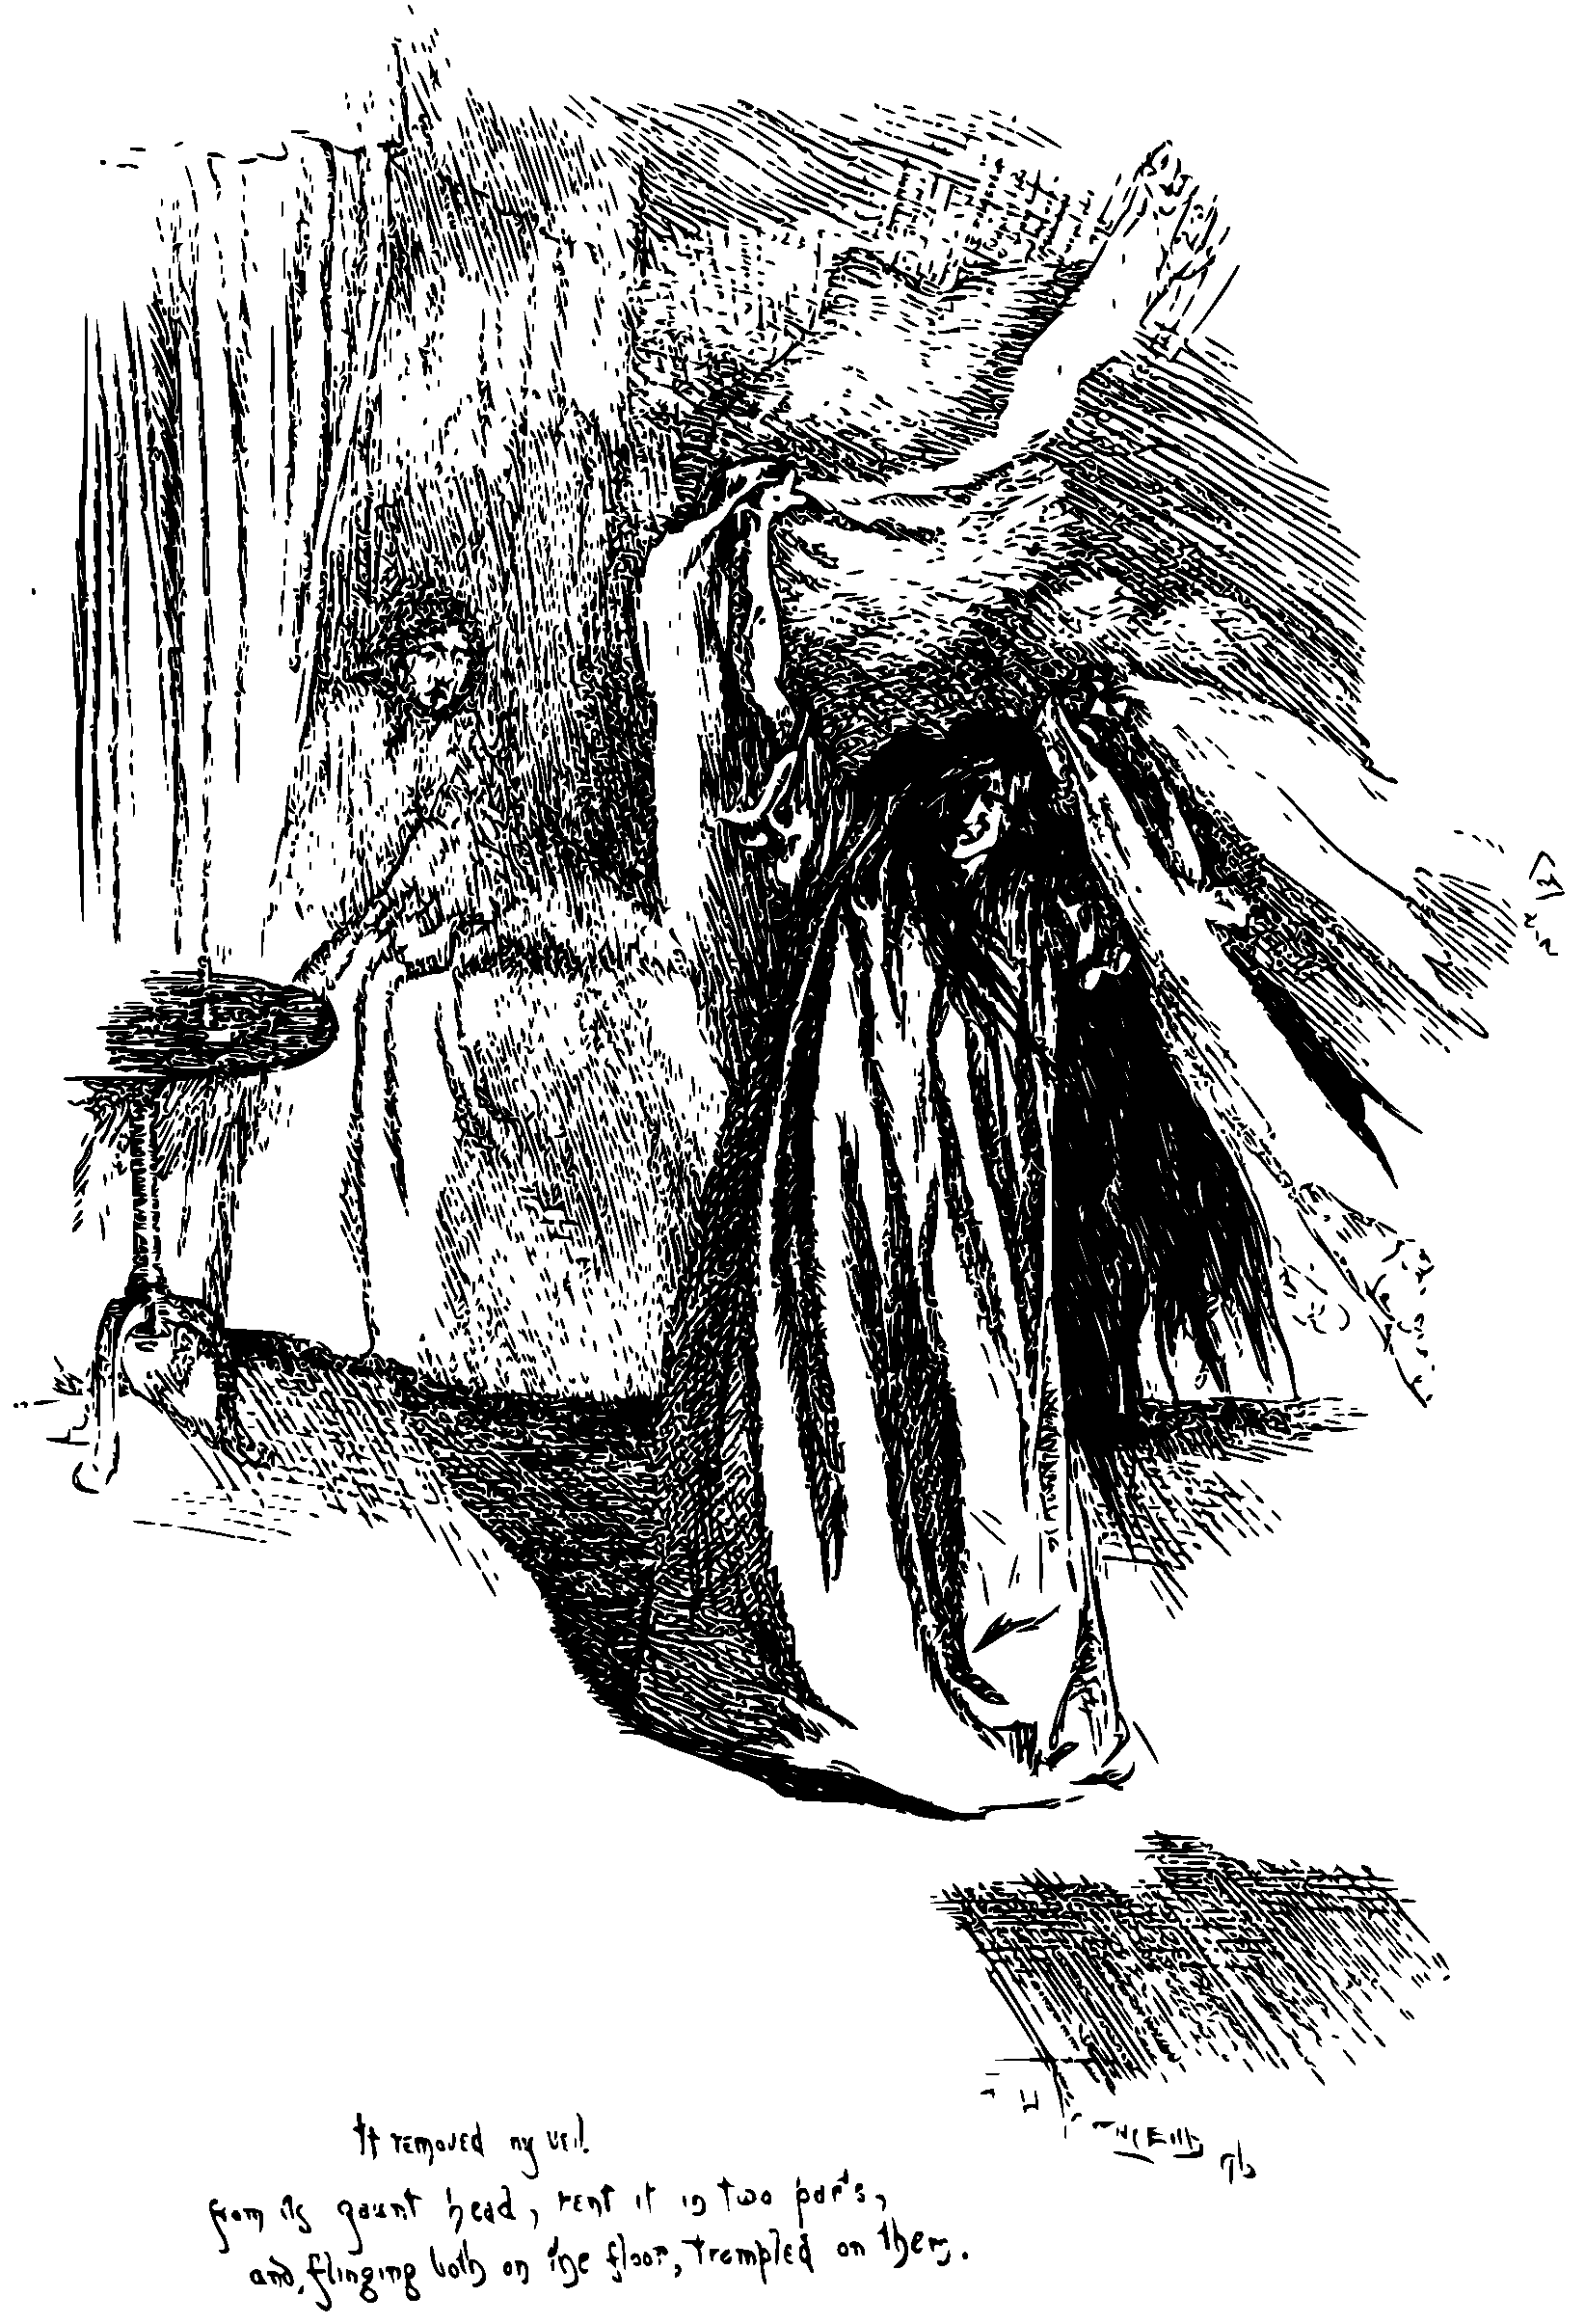
\includegraphics[width=\linewidth]{images/p272b.pdf}
	\end{sidecaption}
\end{figure}

\enquote{Afterwards?}

\enquote{It drew aside the window-curtain and looked out; perhaps it saw
dawn approaching, for, taking the candle, it retreated to the door. 
Just at my bedside, the figure stopped: the fiery eyes glared upon
me---she thrust up her candle close to my face, and extinguished it
under my eyes.  I was aware her lurid visage flamed over mine, and I
lost consciousness: for the second time in my life---only the second
time---I became insensible from terror.}

\enquote{Who was with you when you revived?}

\enquote{No one, sir, but the broad day.  I rose, bathed my head and
face in water, drank a long draught; felt that though enfeebled I was
not ill, and determined that to none but you would I impart this
vision.  Now, sir, tell me who and what that woman was?}

\enquote{The creature of an over-stimulated brain; that is certain.  I
must be careful of you, my treasure: nerves like yours were not made for
rough handling.}

\enquote{Sir, depend on it, my nerves were not in fault; the thing was
real: the transaction actually took place.}

\enquote{And your previous dreams, were they real too?  Is Thornfield
Hall a ruin?  Am I severed from you by insuperable obstacles?  Am I
leaving you without a tear---without a kiss---without a word?}

\enquote{Not yet.}

\enquote{Am I about to do it?  Why, the day is already commenced which
is to bind us indissolubly; and when we are once united, there shall be
no recurrence of these mental terrors: I guarantee that.}

\enquote{Mental terrors, sir!  I wish I could believe them to be only
such: I wish it more now than ever; since even you cannot explain to me
the mystery of that awful visitant.}

\enquote{And since I cannot do it, Jane, it must have been unreal.}

\enquote{But, sir, when I said so to myself on rising this morning, and
when I looked round the room to gather courage and comfort from the
cheerful aspect of each familiar object in full daylight, there---on the
carpet---I saw what gave the distinct lie to my hypothesis,---the veil,
torn from top to bottom in two halves!}

I felt \Mr{} Rochester start and shudder; he hastily flung his arms round
me.  \enquote{Thank God!} he exclaimed, \enquote{that if anything
malignant did come near you last night, it was only the veil that was
harmed.  Oh, to think what might have happened!}

He drew his breath short, and strained me so close to him, I could
scarcely pant.  After some minutes' silence, he continued, cheerily---

\enquote{Now, Janet, I'll explain to you all about it.  It was half
dream, half reality.  A woman did, I doubt not, enter your room: and
that woman was---must have been---Grace Poole.  You call her a strange
being yourself: from all you know, you have reason so to call her---what
did she do to me? what to Mason?  In a state between sleeping and
waking, you noticed her entrance and her actions; but feverish, almost
delirious as you were, you ascribed to her a goblin appearance different
from her own: the long dishevelled hair, the swelled black face, the
exaggerated stature, were figments of imagination; results of nightmare:
the spiteful tearing of the veil was real: and it is like her.  I see
you would ask why I keep such a woman in my house: when we have been
married a year and a day, I will tell you; but not now.  Are you
satisfied, Jane?  Do you accept my solution of the mystery?}

I reflected, and in truth it appeared to me the only possible one:
satisfied I was not, but to please him I endeavoured to appear
so---relieved, I certainly did feel; so I answered him with a contented
smile.  And now, as it was long past one, I prepared to leave him.

\enquote{Does not Sophie sleep with Adèle in the nursery?} he asked, as
I lit my candle.

\enquote{Yes, sir.}

\enquote{And there is room enough in Adèle's little bed for you.  You
must share it with her to-night, Jane: it is no wonder that the incident
you have related should make you nervous, and I would rather you did not
sleep alone: promise me to go to the nursery.}

\enquote{I shall be very glad to do so, sir.}

\enquote{And fasten the door securely on the inside.  Wake Sophie when
you go upstairs, under pretence of requesting her to rouse you in good
time to-morrow; for you must be dressed and have finished breakfast
before eight.  And now, no more sombre thoughts: chase dull care away,
Janet.  Don't you hear to what soft whispers the wind has fallen? and
there is no more beating of rain against the window-panes: look here}
(he lifted up the curtain)---\enquote{it is a lovely night!}

It was.  Half heaven was pure and stainless: the clouds, now trooping
before the wind, which had shifted to the west, were filing off eastward
in long, silvered columns.  The moon shone peacefully.

\enquote{Well,} said \Mr{} Rochester, gazing inquiringly into my eyes,
\enquote{how is my Janet now?}

\enquote{The night is serene, sir; and so am I\@.}

\enquote{And you will not dream of separation and sorrow to-night; but
of happy love and blissful union.}

This prediction was but half fulfilled: I did not indeed dream of
sorrow, but as little did I dream of joy; for I never slept at all. 
With little Adèle in my arms, I watched the slumber of childhood---so
tranquil, so passionless, so innocent---and waited for the coming day:
all my life was awake and astir in my frame: and as soon as the sun rose
I rose too.  I remember Adèle clung to me as I left her: I remember I
kissed her as I loosened her little hands from my neck; and I cried over
her with strange emotion, and quitted her because I feared my sobs would
break her still sound repose.  She seemed the emblem of my past life;
and here I was now to array myself to meet, the dread, but adored, type
of my unknown future day.

\FChapter{Chapter Twenty-Six}{26}

\Lettrine{S}{ophie} \textsc{came} at seven to dress me: she was very long indeed in
accomplishing her task; so long that \Mr{} Rochester, grown, I suppose,
impatient of my delay, sent up to ask why I did not come. She was just
fastening my veil (the plain square of blond after all) to my hair with
a brooch; I hurried from under her hands as soon as I could.

\enquote{Stop!} she cried in French. \enquote{Look at yourself in the
mirror: you have not taken one peep.}

So I turned at the door: I saw a robed and veiled figure, so unlike my
usual self that it seemed almost the image of a stranger. 
\enquote{Jane!} called a voice, and I hastened down. I was received at
the foot of the stairs by \Mr{} Rochester.

\enquote{Lingerer!} he said, \enquote{my brain is on fire with
impatience, and you tarry so long!}

He took me into the dining-room, surveyed me keenly all over, pronounced
me \enquote{fair as a lily, and not only the pride of his life, but the
desire of his eyes,} and then telling me he would give me but ten
minutes to eat some breakfast, he rang the bell. One of his lately
hired servants, a footman, answered it.

\enquote{Is John getting the carriage ready?}

\enquote{Yes, sir.}

\enquote{Is the luggage brought down?}

\enquote{They are bringing it down, sir.}

\enquote{Go you to the church: see if \Mr{} Wood (the clergyman) and the
clerk are there: return and tell me.}

The church, as the reader knows, was but just beyond the gates; the
footman soon returned.

\enquote{\Mr{} Wood is in the vestry, sir, putting on his surplice.}

\enquote{And the carriage?}

\enquote{The horses are harnessing.}

\enquote{We shall not want it to go to church; but it must be ready the
moment we return: all the boxes and luggage arranged and strapped on,
and the coachman in his seat.}

\enquote{Yes, sir.}

\enquote{Jane, are you ready?}

I rose. There were no groomsmen, no bridesmaids, no relatives to wait
for or marshal: none but \Mr{} Rochester and I\@. \Mrs{} Fairfax stood in the
hall as we passed.  I would fain have spoken to her, but my hand was
held by a grasp of iron: I was hurried along by a stride I could hardly
follow; and to look at \Mr{} Rochester's face was to feel that not a
second of delay would be tolerated for any purpose. I wonder what other
bridegroom ever looked as he did---so bent up to a purpose, so grimly
resolute: or who, under such steadfast brows, ever revealed such flaming
and flashing eyes.

I know not whether the day was fair or foul; in descending the drive, I
gazed neither on sky nor earth: my heart was with my eyes; and both
seemed migrated into \Mr{} Rochester's frame. I wanted to see the
invisible thing on which, as we went along, he appeared to fasten a
glance fierce and fell. I wanted to feel the thoughts whose force he
seemed breasting and resisting.

At the churchyard wicket he stopped: he discovered I was quite out of
breath. \enquote{Am I cruel in my love?} he said. \enquote{Delay an
instant: lean on me, Jane.}

And now I can recall the picture of the grey old house of God rising
calm before me, of a rook wheeling round the steeple, of a ruddy morning
sky beyond. I remember something, too, of the green grave-mounds; and I
have not forgotten, either, two figures of strangers straying amongst
the low hillocks and reading the mementoes graven on the few mossy
head-stones. I noticed them, because, as they saw us, they passed round
to the back of the church; and I doubted not they were going to enter by
the side-aisle door and witness the ceremony. By \Mr{} Rochester they
were not observed; he was earnestly looking at my face from which the
blood had, I daresay, momentarily fled: for I felt my forehead dewy, and
my cheeks and lips cold. When I rallied, which I soon did, he walked
gently with me up the path to the porch.

We entered the quiet and humble temple; the priest waited in his white
surplice at the lowly altar, the clerk beside him. All was still: two
shadows only moved in a remote corner. My conjecture had been correct:
the strangers had slipped in before us, and they now stood by the vault
of the Rochesters, their backs towards us, viewing through the rails the
old time-stained marble tomb, where a kneeling angel guarded the remains
of Damer de Rochester, slain at Marston Moor in the time of the civil
wars, and of Elizabeth, his wife.

Our place was taken at the communion rails. Hearing a cautious step
behind me, I glanced over my shoulder: one of the strangers---a
gentleman, evidently---was advancing up the chancel. The service
began. The explanation of the intent of matrimony was gone through; and
then the clergyman came a step further forward, and, bending slightly
towards \Mr{} Rochester, went on.

\enquote{I require and charge you both (as ye will answer at the
dreadful day of judgment, when the secrets of all hearts shall be
disclosed), that if either of you know any impediment why ye may not
lawfully be joined together in matrimony, ye do now confess it; for be
ye well assured that so many as are coupled together otherwise than
God's Word doth allow, are not joined together by God, neither is their
matrimony lawful.}

He paused, as the custom is. When is the pause after that sentence ever
broken by reply? Not, perhaps, once in a hundred years. And the
clergyman, who had not lifted his eyes from his book, and had held his
breath but for a moment, was proceeding: his hand was already stretched
towards \Mr{} Rochester, as his lips unclosed to ask, \enquote{Wilt thou
have this woman for thy wedded wife?}---when a distinct and near voice
said---

\enquote{The marriage cannot go on: I declare the existence of an
impediment.}

The clergyman looked up at the speaker and stood mute; the clerk did the
same; \Mr{} Rochester moved slightly, as if an earthquake had rolled under
his feet: taking a firmer footing, and not turning his head or eyes, he
said, \enquote{Proceed.}

Profound silence fell when he had uttered that word, with deep but low
intonation. Presently \Mr{} Wood said---

\enquote{I cannot proceed without some investigation into what has been
asserted, and evidence of its truth or falsehood.}

\enquote{The ceremony is quite broken off,} subjoined the voice behind
us. \enquote{I am in a condition to prove my allegation: an insuperable
impediment to this marriage exists.}

\Mr{} Rochester heard, but heeded not: he stood stubborn and rigid, making
no movement but to possess himself of my hand. What a hot and strong
grasp he had! and how like quarried marble was his pale, firm, massive
front at this moment! How his eye shone, still watchful, and yet wild
beneath!

\Mr{} Wood seemed at a loss. \enquote{What is the nature of the
impediment?} he asked. \enquote{Perhaps it may be got over---explained
away?}

\enquote{Hardly,} was the answer. \enquote{I have called it
insuperable, and I speak advisedly.}

The speaker came forward and leaned on the rails. He continued,
uttering each word distinctly, calmly, steadily, but not loudly---

\enquote{It simply consists in the existence of a previous marriage. 
\Mr{} Rochester has a wife now living.}

My nerves vibrated to those low-spoken words as they had never vibrated
to thunder---my blood felt their subtle violence as it had never felt
frost or fire; but I was collected, and in no danger of swooning. I
looked at \Mr{} Rochester: I made him look at me. His whole face was
colourless rock: his eye was both spark and flint. He disavowed
nothing: he seemed as if he would defy all things. Without speaking,
without smiling, without seeming to recognise in me a human being, he
only twined my waist with his arm and riveted me to his side.

\enquote{Who are you?} he asked of the intruder.

\enquote{My name is Briggs, a solicitor of --- Street, London.}

\enquote{And you would thrust on me a wife?}

\enquote{I would remind you of your lady's existence, sir, which the law
recognises, if you do not.}

\enquote{Favour me with an account of her---with her name, her
parentage, her place of abode.}

\enquote{Certainly.} \Mr{} Briggs calmly took a paper from his pocket,
and read out in a sort of official, nasal voice:---

\enquote{\enquote{I affirm and can prove that on the 20th of October
\AD{} --- (a date of fifteen years back), Edward Fairfax Rochester, of
Thornfield Hall, in the county of ---, and of Ferndean Manor, in
---shire, England, was married to my sister, Bertha Antoinetta Mason,
daughter of Jonas Mason, merchant, and of Antoinetta his wife, a Creole,
at --- church, Spanish Town, Jamaica. The record of the marriage will
be found in the register of that church---a copy of it is now in my
possession. Signed, Richard Mason.}}

\enquote{That---if a genuine document---may prove I have been married,
but it does not prove that the woman mentioned therein as my wife is
still living.}

\enquote{She was living three months ago,} returned the lawyer.

\enquote{How do you know?}

\enquote{I have a witness to the fact, whose testimony even you, sir,
will scarcely controvert.}

\enquote{Produce him---or go to hell.}

\enquote{I will produce him first---he is on the spot. \Mr{} Mason, have
the goodness to step forward.}

\Mr{} Rochester, on hearing the name, set his teeth; he experienced, too,
a sort of strong convulsive quiver; near to him as I was, I felt the
spasmodic movement of fury or despair run through his frame. The second
stranger, who had hitherto lingered in the background, now drew near; a
pale face looked over the solicitor's shoulder---yes, it was Mason
himself. \Mr{} Rochester turned and glared at him. His eye, as I have
often said, was a black eye: it had now a tawny, nay, a bloody light in
its gloom; and his face flushed---olive cheek and hueless forehead
received a glow as from spreading, ascending heart-fire: and he stirred,
lifted his strong arm---he could have struck Mason, dashed him on the
church-floor, shocked by ruthless blow the breath from his body---but
Mason shrank away, and cried faintly, \enquote{Good God!} Contempt fell
cool on \Mr{} Rochester---his passion died as if a blight had shrivelled
it up: he only asked---\enquote{What have \emph{you} to say?}

An inaudible reply escaped Mason's white lips.

\enquote{The devil is in it if you cannot answer distinctly. I again
demand, what have you to say?}

\enquote{Sir---sir,} interrupted the clergyman, \enquote{do not forget
you are in a sacred place.} Then addressing Mason, he inquired gently,
\enquote{Are you aware, sir, whether or not this gentleman's wife is
still living?}

\enquote{Courage,} urged the lawyer,---\enquote{speak out.}

\enquote{She is now living at Thornfield Hall,} said Mason, in more
articulate tones: \enquote{I saw her there last April. I am her
brother.}

\enquote{At Thornfield Hall!} ejaculated the clergyman. 
\enquote{Impossible! I am an old resident in this neighbourhood, sir,
and I never heard of a \Mrs{} Rochester at Thornfield Hall.}

I saw a grim smile contort \Mr{} Rochester's lips, and he muttered---

\enquote{No, by God! I took care that none should hear of it---or of
her under that name.} He mused---for ten minutes he held counsel with
himself: he formed his resolve, and announced it---

\enquote{Enough! all shall bolt out at once, like the bullet from the
barrel. Wood, close your book and take off your surplice; John Green
(to the clerk), leave the church: there will be no wedding to-day.} The
man obeyed.

\Mr{} Rochester continued, hardily and recklessly: \enquote{Bigamy is an ugly
word!---I meant, however, to be a bigamist; but fate has out-manoeuvred
me, or Providence has checked me,---perhaps the last. I am little
better than a devil at this moment; and, as my pastor there would tell
me, deserve no doubt the sternest judgments of God, even to the
quenchless fire and deathless worm. Gentlemen, my plan is broken
up:---what this lawyer and his client say is true: I have been married,
and the woman to whom I was married lives! You say you never heard of a
\Mrs{} Rochester at the house up yonder, Wood; but I daresay you have many
a time inclined your ear to gossip about the mysterious lunatic kept
there under watch and ward. Some have whispered to you that she is my
bastard half-sister: some, my cast-off mistress. I now inform you that
she is my wife, whom I married fifteen years ago,---Bertha Mason by
name; sister of this resolute personage, who is now, with his quivering
limbs and white cheeks, showing you what a stout heart men may bear. 
Cheer up, Dick!---never fear me!---I'd almost as soon strike a woman as
you. Bertha Mason is mad; and she came of a mad family; idiots and
maniacs through three generations! Her mother, the Creole, was both a
madwoman and a drunkard!---as I found out after I had wed the daughter:
for they were silent on family secrets before. Bertha, like a dutiful
child, copied her parent in both points. I had a charming
partner---pure, wise, modest: you can fancy I was a happy man. I went
through rich scenes! Oh! my experience has been heavenly, if you only
knew it! But I owe you no further explanation. Briggs, Wood, Mason, I
invite you all to come up to the house and visit \Mrs{} Poole's patient,
and \emph{my wife}! You shall see what sort of a being I was cheated
into espousing, and judge whether or not I had a right to break the
compact, and seek sympathy with something at least human. This girl,}
he continued, looking at me, \enquote{knew no more than you, Wood, of
the disgusting secret: she thought all was fair and legal and never
dreamt she was going to be entrapped into a feigned union with a
defrauded wretch, already bound to a bad, mad, and embruted partner! 
Come all of you---follow!}

Still holding me fast, he left the church: the three gentlemen came
after. At the front door of the hall we found the carriage.

\enquote{Take it back to the coach-house, John,} said \Mr{} Rochester
coolly; \enquote{it will not be wanted to-day.}

At our entrance, \Mrs{} Fairfax, Adèle, Sophie, Leah, advanced to meet and
greet us.

\enquote{To the right-about---every soul!} cried the master;
\enquote{away with your congratulations! Who wants them? Not I!---they
are fifteen years too late!}

He passed on and ascended the stairs, still holding my hand, and still
beckoning the gentlemen to follow him, which they did. We mounted the
first staircase, passed up the gallery, proceeded to the third storey:
the low, black door, opened by \Mr{} Rochester's master-key, admitted us
to the tapestried room, with its great bed and its pictorial cabinet.

\enquote{You know this place, Mason,} said our guide; \enquote{she bit
and stabbed you here.}

He lifted the hangings from the wall, uncovering the second door: this,
too, he opened. In a room without a window, there burnt a fire guarded
by a high and strong fender, and a lamp suspended from the ceiling by a
chain. Grace Poole bent over the fire, apparently cooking something in
a saucepan. In the deep shade, at the farther end of the room, a figure
ran backwards and forwards. What it was, whether beast or human being,
one could not, at first sight, tell: it grovelled, seemingly, on all
fours; it snatched and growled like some strange wild animal: but it was
covered with clothing, and a quantity of dark, grizzled hair, wild as a
mane, hid its head and face.

\enquote{Good-morrow, \Mrs{} Poole!} said \Mr{} Rochester. \enquote{How are
you? and how is your charge to-day?}

\enquote{We're tolerable, sir, I thank you,} replied Grace, lifting the
boiling mess carefully on to the hob: \enquote{rather snappish, but not
'rageous.}

A fierce cry seemed to give the lie to her favourable report: the
clothed hyena rose up, and stood tall on its hind-feet.

\enquote{Ah! sir, she sees you!} exclaimed Grace: \enquote{you'd better
not stay.}

\enquote{Only a few moments, Grace: you must allow me a few moments.}

\enquote{Take care then, sir!---for God's sake, take care!}

The maniac bellowed: she parted her shaggy locks from her visage, and
gazed wildly at her visitors. I recognised well that purple
face,---those bloated features. \Mrs{} Poole advanced.

\enquote{Keep out of the way,} said \Mr{} Rochester, thrusting her aside:
\enquote{she has no knife now, I suppose, and I'm on my guard.}

\enquote{One never knows what she has, sir: she is so cunning: it is not
in mortal discretion to fathom her craft.}

\enquote{We had better leave her,} whispered Mason.

\enquote{Go to the devil!} was his brother-in-law's recommendation.

\enquote{'Ware!} cried Grace. The three gentlemen retreated
simultaneously. \Mr{} Rochester flung me behind him: the lunatic sprang
and grappled his throat viciously, and laid her teeth to his cheek: they
struggled. She was a big woman, in stature almost equalling her
husband, and corpulent besides: she showed virile force in the
contest---more than once she almost throttled him, athletic as he was. 
He could have settled her with a well-planted blow; but he would not
strike: he would only wrestle. At last he mastered her arms; Grace
Poole gave him a cord, and he pinioned them behind her: with more rope,
which was at hand, he bound her to a chair. The operation was performed
amidst the fiercest yells and the most convulsive plunges. \Mr{}
 Rochester then turned to the spectators: he looked at them with a smile
both acrid and desolate.

\enquote{That is \emph{my wife},} said he. \enquote{Such is the sole conjugal
embrace I am ever to know---such are the endearments which are to solace
my leisure hours! And \emph{this} is what I wished to have} (laying
his hand on my shoulder): \enquote{this young girl, who stands so grave
and quiet at the mouth of hell, looking collectedly at the gambols of a
demon, I wanted her just as a change after that fierce ragout. Wood and
Briggs, look at the difference! Compare these clear eyes with the red
balls yonder---this face with that mask---this form with that bulk; then
judge me, priest of the gospel and man of the law, and remember with
what judgment ye judge ye shall be judged! Off with you now. I must
shut up my prize.}

We all withdrew. \Mr{} Rochester stayed a moment behind us, to give some
further order to Grace Poole. The solicitor addressed me as he
descended the stair.

\enquote{You, madam,} said he, \enquote{are cleared from all blame: your
uncle will be glad to hear it---if, indeed, he should be still
living---when \Mr{} Mason returns to Madeira.}

\enquote{My uncle! What of him? Do you know him?}

\enquote{\Mr{} Mason does. \Mr{} Eyre has been the Funchal correspondent of
his house for some years. When your uncle received your letter
intimating the contemplated union between yourself and \Mr{} Rochester,
\Mr{} Mason, who was staying at Madeira to recruit his health, on his way
back to Jamaica, happened to be with him. \Mr{} Eyre mentioned the
intelligence; for he knew that my client here was acquainted with a
gentleman of the name of Rochester. \Mr{} Mason, astonished and
distressed as you may suppose, revealed the real state of matters. Your
uncle, I am sorry to say, is now on a sick bed; from which, considering
the nature of his disease---decline---and the stage it has reached, it
is unlikely he will ever rise. He could not then hasten to England
himself, to extricate you from the snare into which you had fallen, but
he implored \Mr{} Mason to lose no time in taking steps to prevent the
false marriage. He referred him to me for assistance. I used all
despatch, and am thankful I was not too late: as you, doubtless, must be
also. Were I not morally certain that your uncle will be dead ere you
reach Madeira, I would advise you to accompany \Mr{} Mason back; but as it
is, I think you had better remain in England till you can hear further,
either from or of \Mr{} Eyre. Have we anything else to stay for?} he
inquired of \Mr{} Mason.

\enquote{No, no---let us be gone,} was the anxious reply; and without
waiting to take leave of \Mr{} Rochester, they made their exit at the hall
door. The clergyman stayed to exchange a few sentences, either of
admonition or reproof, with his haughty parishioner; this duty done, he
too departed.

I heard him go as I stood at the half-open door of my own room, to which
I had now withdrawn. The house cleared, I shut myself in, fastened the
bolt that none might intrude, and proceeded---not to weep, not to mourn,
I was yet too calm for that, but---mechanically to take off the wedding
dress, and replace it by the stuff gown I had worn yesterday, as I
thought, for the last time. I then sat down: I felt weak and tired. I
leaned my arms on a table, and my head dropped on them. And now I
thought: till now I had only heard, seen, moved---followed up and down
where I was led or dragged---watched event rush on event, disclosure
open beyond disclosure: but \emph{now}, \emph{I thought}.

The morning had been a quiet morning enough---all except the brief scene
with the lunatic: the transaction in the church had not been noisy;
there was no explosion of passion, no loud altercation, no dispute, no
defiance or challenge, no tears, no sobs: a few words had been spoken, a
calmly pronounced objection to the marriage made; some stern, short
questions put by \Mr{} Rochester; answers, explanations given, evidence
adduced; an open admission of the truth had been uttered by my master;
then the living proof had been seen; the intruders were gone, and all
was over.

I was in my own room as usual---just myself, without obvious change:
nothing had smitten me, or scathed me, or maimed me. And yet where was
the Jane Eyre of yesterday?---where was her life?---where were her
prospects?

Jane Eyre, who had been an ardent, expectant woman---almost a bride, was
a cold, solitary girl again: her life was pale; her prospects were
desolate. A Christmas frost had come at midsummer; a white December
storm had whirled over June; ice glazed the ripe apples, drifts crushed
the blowing roses; on hayfield and cornfield lay a frozen shroud: lanes
which last night blushed full of flowers, to-day were pathless with
untrodden snow; and the woods, which twelve hours since waved leafy and
flagrant as groves between the tropics, now spread, waste, wild, and
white as pine-forests in wintry Norway. My hopes were all dead---struck
with a subtle doom, such as, in one night, fell on all the first-born in
the land of Egypt. I looked on my cherished wishes, yesterday so
blooming and glowing; they lay stark, chill, livid corpses that could
never revive. I looked at my love: that feeling which was my
master's---which he had created; it shivered in my heart, like a
suffering child in a cold cradle; sickness and anguish had seized it; it
could not seek \Mr{} Rochester's arms---it could not derive warmth from
his breast. Oh, never more could it turn to him; for faith was
blighted---confidence destroyed! \Mr{} Rochester was not to me what he
had been; for he was not what I had thought him. I would not ascribe
vice to him; I would not say he had betrayed me; but the attribute of
stainless truth was gone from his idea, and from his presence I must go:
\emph{that} I perceived well. When---how---whither, I could not yet
discern; but he himself, I doubted not, would hurry me from Thornfield. 
Real affection, it seemed, he could not have for me; it had been only
fitful passion: that was balked; he would want me no more. I should
fear even to cross his path now: my view must be hateful to him. Oh,
how blind had been my eyes! How weak my conduct!

My eyes were covered and closed: eddying darkness seemed to swim round
me, and reflection came in as black and confused a flow. 
Self-abandoned, relaxed, and effortless, I seemed to have laid me down
in the dried-up bed of a great river; I heard a flood loosened in remote
mountains, and felt the torrent come: to rise I had no will, to flee I
had no strength. I lay faint, longing to be dead. One idea only still
throbbed life-like within me---a remembrance of God: it begot an
unuttered prayer: these words went wandering up and down in my rayless
mind, as something that should be whispered, but no energy was found to
express them---

\enquote{Be not far from me, for trouble is near: there is none to
help.}

It was near: and as I had lifted no petition to Heaven to avert it---as
I had neither joined my hands, nor bent my knees, nor moved my lips---it
came: in full heavy swing the torrent poured over me. The whole
consciousness of my life lorn, my love lost, my hope quenched, my faith
death-struck, swayed full and mighty above me in one sullen mass. That
bitter hour cannot be described: in truth, \enquote{the waters came into
my soul; I sank in deep mire: I felt no standing; I came into deep
waters; the floods overflowed me.}

\FChapter{Chapter Twenty-Seven}{27}

\Lettrine{S}{ome} \textsc{time} in the afternoon I raised my head, and looking round and
seeing the western sun gilding the sign of its decline on the wall, I
asked, \enquote{What am I to do?}

\zz
But the answer my mind gave---\enquote{Leave Thornfield at once}---was
so prompt, so dread, that I stopped my ears. I said I could not bear
such words now. \enquote{That I am not Edward Rochester's bride is the
least part of my woe,} I alleged: \enquote{that I have wakened out of
most glorious dreams, and found them all void and vain, is a horror I
could bear and master; but that I must leave him decidedly, instantly,
entirely, is intolerable. I cannot do it.}

But, then, a voice within me averred that I could do it and foretold
that I should do it. I wrestled with my own resolution: I wanted to be
weak that I might avoid the awful passage of further suffering I saw
laid out for me; and Conscience, turned tyrant, held Passion by the
throat, told her tauntingly, she had yet but dipped her dainty foot in
the slough, and swore that with that arm of iron he would thrust her
down to unsounded depths of agony.

\enquote{Let me be torn away,} then I cried. \enquote{Let another help
me!}

\enquote{No; you shall tear yourself away, none shall help you: you
shall yourself pluck out your right eye; yourself cut off your right
hand: your heart shall be the victim, and you the priest to transfix
it.}

I rose up suddenly, terror-struck at the solitude which so ruthless a
judge haunted,---at the silence which so awful a voice filled. My head
swam as I stood erect. I perceived that I was sickening from excitement
and inanition; neither meat nor drink had passed my lips that day, for I
had taken no breakfast. And, with a strange pang, I now reflected that,
long as I had been shut up here, no message had been sent to ask how I
was, or to invite me to come down: not even little Adèle had tapped at
the door; not even \Mrs{} Fairfax had sought me. \enquote{Friends always
forget those whom fortune forsakes,} I murmured, as I undrew the bolt
and passed out. I stumbled over an obstacle: my head was still dizzy,
my sight was dim, and my limbs were feeble. I could not soon recover
myself. I fell, but not on to the ground: an outstretched arm caught
me. I looked up---I was supported by \Mr{} Rochester, who sat in a chair
across my chamber threshold.

\enquote{You come out at last,} he said. \enquote{Well, I have been
waiting for you long, and listening: yet not one movement have I heard,
nor one sob: five minutes more of that death-like hush, and I should
have forced the lock like a burglar. So you shun me?---you shut
yourself up and grieve alone! I would rather you had come and upbraided
me with vehemence. You are passionate. I expected a scene of some
kind. I was prepared for the hot rain of tears; only I wanted them to
be shed on my breast: now a senseless floor has received them, or your
drenched handkerchief. But I err: you have not wept at all! I see a
white cheek and a faded eye, but no trace of tears. I suppose, then,
your heart has been weeping blood?}

\enquote{Well, Jane! not a word of reproach? Nothing bitter---nothing
poignant? Nothing to cut a feeling or sting a passion? You sit quietly
where I have placed you, and regard me with a weary, passive look.}

\enquote{Jane, I never meant to wound you thus. If the man who had but
one little ewe lamb that was dear to him as a daughter, that ate of his
bread and drank of his cup, and lay in his bosom, had by some mistake
slaughtered it at the shambles, he would not have rued his bloody
blunder more than I now rue mine. Will you ever forgive me?}

Reader, I forgave him at the moment and on the spot. There was such
deep remorse in his eye, such true pity in his tone, such manly energy
in his manner; and besides, there was such unchanged love in his whole
look and mien---I forgave him all: yet not in words, not outwardly; only
at my heart's core.

\enquote{You know I am a scoundrel, Jane?} ere long he inquired
wistfully---wondering, I suppose, at my continued silence and tameness,
the result rather of weakness than of will.

\enquote{Yes, sir.}

\enquote{Then tell me so roundly and sharply---don't spare me.}

\enquote{I cannot: I am tired and sick. I want some water.} He heaved
a sort of shuddering sigh, and taking me in his arms, carried me
downstairs. At first I did not know to what room he had borne me; all
was cloudy to my glazed sight: presently I felt the reviving warmth of a
fire; for, summer as it was, I had become icy cold in my chamber. He
put wine to my lips; I tasted it and revived; then I ate something he
offered me, and was soon myself. I was in the library---sitting in his
chair---he was quite near. \enquote{If I could go out of life now,
without too sharp a pang, it would be well for me,} I thought;
\enquote{then I should not have to make the effort of cracking my
heart-strings in rending them from among \Mr{} Rochester's. I must leave
him, it appears. I do not want to leave him---I cannot leave him.}

\enquote{How are you now, Jane?}

\enquote{Much better, sir; I shall be well soon.}

\enquote{Taste the wine again, Jane.}

I obeyed him; then he put the glass on the table, stood before me, and
looked at me attentively. Suddenly he turned away, with an inarticulate
exclamation, full of passionate emotion of some kind; he walked fast
through the room and came back; he stooped towards me as if to kiss me;
but I remembered caresses were now forbidden. I turned my face away and
put his aside.

\enquote{What!---How is this?} he exclaimed hastily. \enquote{Oh, I
know! you won't kiss the husband of Bertha Mason? You consider my arms
filled and my embraces appropriated?}

\enquote{At any rate, there is neither room nor claim for me, sir.}

\enquote{Why, Jane? I will spare you the trouble of much talking; I
will answer for you---Because I have a wife already, you would
reply.---I guess rightly?}

\enquote{Yes.}

\enquote{If you think so, you must have a strange opinion of me; you must
regard me as a plotting profligate---a base and low rake who has been
simulating disinterested love in order to draw you into a snare
deliberately laid, and strip you of honour and rob you of self-respect. 
What do you say to that? I see you can say nothing in the first place,
you are faint still, and have enough to do to draw your breath; in the
second place, you cannot yet accustom yourself to accuse and revile me,
and besides, the flood-gates of tears are opened, and they would rush
out if you spoke much; and you have no desire to expostulate, to
upbraid, to make a scene: you are thinking how \emph{to
act}---\emph{talking} you consider is of no use. I know you---I am on
my guard.}

\enquote{Sir, I do not wish to act against you,} I said; and my unsteady
voice warned me to curtail my sentence.

\enquote{Not in your sense of the word, but in mine you are scheming to
destroy me. You have as good as said that I am a married man---as a
married man you will shun me, keep out of my way: just now you have
refused to kiss me. You intend to make yourself a complete stranger to
me: to live under this roof only as Adèle's governess; if ever I say a
friendly word to you, if ever a friendly feeling inclines you again to
me, you will say,---\enquote{That man had nearly made me his mistress: I must be
ice and rock to him;} and ice and rock you will accordingly become.}

I cleared and steadied my voice to reply: \enquote{All is changed about
me, sir; I must change too---there is no doubt of that; and to avoid
fluctuations of feeling, and continual combats with recollections and
associations, there is only one way---Adèle must have a new governess,
sir.}

\enquote{Oh, Adèle will go to school---I have settled that already; nor do I
mean to torment you with the hideous associations and recollections of
Thornfield Hall---this accursed place---this tent of Achan---this
insolent vault, offering the ghastliness of living death to the light of
the open sky---this narrow stone hell, with its one real fiend, worse
than a legion of such as we imagine. Jane, you shall not stay here, nor
will I\@. I was wrong ever to bring you to Thornfield Hall, knowing as I
did how it was haunted. I charged them to conceal from you, before I
ever saw you, all knowledge of the curse of the place; merely because I
feared Adèle never would have a governess to stay if she knew with what
inmate she was housed, and my plans would not permit me to remove the
maniac elsewhere---though I possess an old house, Ferndean Manor, even
more retired and hidden than this, where I could have lodged her safely
enough, had not a scruple about the unhealthiness of the situation, in
the heart of a wood, made my conscience recoil from the arrangement. 
Probably those damp walls would soon have eased me of her charge: but to
each villain his own vice; and mine is not a tendency to indirect
assassination, even of what I most hate.

%rem enq
Concealing the mad-woman's neighbourhood from you, however, was
something like covering a child with a cloak and laying it down near a
upas-tree: that demon's vicinage is poisoned, and always was. But I'll
shut up Thornfield Hall: I'll nail up the front door and board the lower
windows: I'll give \Mrs{} Poole two hundred a year to live here with
\emph{my wife}, as you term that fearful hag: Grace will do much for
money, and she shall have her son, the keeper at Grimsby Retreat, to
bear her company and be at hand to give her aid in the paroxysms, when
\emph{my wife} is prompted by her familiar to burn people in their beds
at night, to stab them, to bite their flesh from their bones, and so
on---}

\enquote{Sir,} I interrupted him, \enquote{you are inexorable for that
unfortunate lady: you speak of her with hate---with vindictive
antipathy. It is cruel---she cannot help being mad.}

\enquote{Jane, my little darling (so I will call you, for so you are),
you don't know what you are talking about; you misjudge me again: it is
not because she is mad I hate her. If you were mad, do you think I
should hate you?}

\enquote{I do indeed, sir.}

\enquote{Then you are mistaken, and you know nothing about me, and
nothing about the sort of love of which I am capable. Every atom of
your flesh is as dear to me as my own: in pain and sickness it would
still be dear. Your mind is my treasure, and if it were broken, it
would be my treasure still: if you raved, my arms should confine you,
and not a strait waistcoat---your grasp, even in fury, would have a
charm for me: if you flew at me as wildly as that woman did this
morning, I should receive you in an embrace, at least as fond as it
would be restrictive. I should not shrink from you with disgust as I
did from her: in your quiet moments you should have no watcher and no
nurse but me; and I could hang over you with untiring tenderness, though
you gave me no smile in return; and never weary of gazing into your
eyes, though they had no longer a ray of recognition for me.---But why
do I follow that train of ideas? I was talking of removing you from
Thornfield. All, you know, is prepared for prompt departure: to-morrow
you shall go. I only ask you to endure one more night under this roof,
Jane; and then, farewell to its miseries and terrors for ever! I have a
place to repair to, which will be a secure sanctuary from hateful
reminiscences, from unwelcome intrusion---even from falsehood and
slander.}

\enquote{And take Adèle with you, sir,} I interrupted; \enquote{she will
be a companion for you.}

\enquote{What do you mean, Jane? I told you I would send Adèle to
school; and what do I want with a child for a companion, and not my own
child,---a French dancer's bastard? Why do you importune me about her! 
I say, why do you assign Adèle to me for a companion?}

\enquote{You spoke of a retirement, sir; and retirement and solitude are
dull: too dull for you.}

\enquote{Solitude! solitude!} he reiterated with irritation. \enquote{I
see I must come to an explanation. I don't know what sphynx-like
expression is forming in your countenance. You are to share my
solitude. Do you understand?}

I shook my head: it required a degree of courage, excited as he was
becoming, even to risk that mute sign of dissent. He had been walking
fast about the room, and he stopped, as if suddenly rooted to one spot. 
He looked at me long and hard: I turned my eyes from him, fixed them on
the fire, and tried to assume and maintain a quiet, collected aspect.

\enquote{Now for the hitch in Jane's character,} he said at last,
speaking more calmly than from his look I had expected him to speak. 
\enquote{The reel of silk has run smoothly enough so far; but I always
knew there would come a knot and a puzzle: here it is. Now for
vexation, and exasperation, and endless trouble! By God! I long to
exert a fraction of Samson's strength, and break the entanglement like
tow!}

He recommenced his walk, but soon again stopped, and this time just
before me.

\enquote{Jane! will you hear reason?} (he stooped and approached his
lips to my ear); \enquote{because, if you won't, I'll try violence.} 
His voice was hoarse; his look that of a man who is just about to burst
an insufferable bond and plunge headlong into wild license. I saw that
in another moment, and with one impetus of frenzy more, I should be able
to do nothing with him. The present---the passing second of time---was
all I had in which to control and restrain him---a movement of
repulsion, flight, fear would have sealed my doom,---and his. But I was
not afraid: not in the least. I felt an inward power; a sense of
influence, which supported me. The crisis was perilous; but not without
its charm: such as the Indian, perhaps, feels when he slips over the
rapid in his canoe. I took hold of his clenched hand, loosened the
contorted fingers, and said to him, soothingly---

\enquote{Sit down; I'll talk to you as long as you like, and hear all
you have to say, whether reasonable or unreasonable.}

He sat down: but he did not get leave to speak directly. I had been
struggling with tears for some time: I had taken great pains to repress
them, because I knew he would not like to see me weep. Now, however, I
considered it well to let them flow as freely and as long as they
liked. If the flood annoyed him, so much the better. So I gave way and
cried heartily.

Soon I heard him earnestly entreating me to be composed. I said I could
not while he was in such a passion.

\enquote{But I am not angry, Jane: I only love you too well; and you had
steeled your little pale face with such a resolute, frozen look, I could
not endure it. Hush, now, and wipe your eyes.}

His softened voice announced that he was subdued; so I, in my turn,
became calm. Now he made an effort to rest his head on my shoulder, but
I would not permit it. Then he would draw me to him: no.

\enquote{Jane! Jane!} he said, in such an accent of bitter sadness it
thrilled along every nerve I had; \enquote{you don't love me, then? It
was only my station, and the rank of my wife, that you valued? Now that
you think me disqualified to become your husband, you recoil from my
touch as if I were some toad or ape.}

These words cut me: yet what could I do or I say? I ought probably to
have done or said nothing; but I was so tortured by a sense of remorse
at thus hurting his feelings, I could not control the wish to drop balm
where I had wounded.

\enquote{I \emph{do} love you,} I said, \enquote{more than ever: but I must
not show or indulge the feeling: and this is the last time I must
express it.}

\enquote{The last time, Jane! What! do you think you can live with me,
and see me daily, and yet, if you still love me, be always cold and
distant?}

\enquote{No, sir; that I am certain I could not; and therefore I see
there is but one way: but you will be furious if I mention it.}

\enquote{Oh, mention it! If I storm, you have the art of weeping.}

\enquote{\Mr{} Rochester, I must leave you.}

\enquote{For how long, Jane? For a few minutes, while you smooth your
hair---which is somewhat dishevelled; and bathe your face---which looks
feverish?}

\enquote{I must leave Adèle and Thornfield. I must part with you for my
whole life: I must begin a new existence among strange faces and strange
scenes.}

\enquote{Of course: I told you you should. I pass over the madness
about parting from me. You mean you must become a part of me. As to
the new existence, it is all right: you shall yet be my wife: I am not
married. You shall be \Mrs{} Rochester---both virtually and nominally. I
shall keep only to you so long as you and I live. You shall go to a
place I have in the south of France: a whitewashed villa on the shores
of the Mediterranean. There you shall live a happy, and guarded, and
most innocent life. Never fear that I wish to lure you into error---to
make you my mistress. Why did you shake your head? Jane, you must be
reasonable, or in truth I shall again become frantic.}

His voice and hand quivered: his large nostrils dilated; his eye blazed:
still I dared to speak.

\enquote{Sir, your wife is living: that is a fact acknowledged this
morning by yourself. If I lived with you as you desire, I should then
be your mistress: to say otherwise is sophistical---is false.}

\enquote{Jane, I am not a gentle-tempered man---you forget that: I am
not long-enduring; I am not cool and dispassionate. Out of pity to me
and yourself, put your finger on my pulse, feel how it throbs,
and---beware!}

He bared his wrist, and offered it to me: the blood was forsaking his
cheek and lips, they were growing livid; I was distressed on all hands. 
To agitate him thus deeply, by a resistance he so abhorred, was cruel:
to yield was out of the question. I did what human beings do
instinctively when they are driven to utter extremity---looked for aid
to one higher than man: the words \enquote{God help me!} burst
involuntarily from my lips.

\enquote{I am a fool!} cried \Mr{} Rochester suddenly. \enquote{I keep
telling her I am not married, and do not explain to her why. I forget
she knows nothing of the character of that woman, or of the
circumstances attending my infernal union with her. Oh, I am certain
Jane will agree with me in opinion, when she knows all that I know! 
Just put your hand in mine, Janet---that I may have the evidence of
touch as well as sight, to prove you are near me---and I will in a few
words show you the real state of the case. Can you listen to me?}

\enquote{Yes, sir; for hours if you will.}

\enquote{I ask only minutes. Jane, did you ever hear or know that I was
not the eldest son of my house: that I had once a brother older than I?}

\enquote{I remember \Mrs{} Fairfax told me so once.}

\enquote{And did you ever hear that my father was an avaricious,
grasping man?}

\enquote{I have understood something to that effect.}

\enquote{Well, Jane, being so, it was his resolution to keep the
property together; he could not bear the idea of dividing his estate and
leaving me a fair portion: all, he resolved, should go to my brother,
Rowland. Yet as little could he endure that a son of his should be a
poor man. I must be provided for by a wealthy marriage. He sought me a
partner betimes. \Mr{} Mason, a West India planter and merchant, was his
old acquaintance. He was certain his possessions were real and vast: he
made inquiries. \Mr{} Mason, he found, had a son and daughter; and he
learned from him that he could and would give the latter a fortune of
thirty thousand pounds: that sufficed. When I left college, I was sent
out to Jamaica, to espouse a bride already courted for me. My father
said nothing about her money; but he told me Miss Mason was the boast of
Spanish Town for her beauty: and this was no lie. I found her a fine
woman, in the style of Blanche Ingram: tall, dark, and majestic. Her
family wished to secure me because I was of a good race; and so did
she. They showed her to me in parties, splendidly dressed. I seldom
saw her alone, and had very little private conversation with her. She
flattered me, and lavishly displayed for my pleasure her charms and
accomplishments. All the men in her circle seemed to admire her and
envy me. I was dazzled, stimulated: my senses were excited; and being
ignorant, raw, and inexperienced, I thought I loved her. There is no
folly so besotted that the idiotic rivalries of society, the prurience,
the rashness, the blindness of youth, will not hurry a man to its
commission. Her relatives encouraged me; competitors piqued me; she
allured me: a marriage was achieved almost before I knew where I was. 
Oh, I have no respect for myself when I think of that act!---an agony of
inward contempt masters me. I never loved, I never esteemed, I did not
even know her. I was not sure of the existence of one virtue in her
nature: I had marked neither modesty, nor benevolence, nor candour, nor
refinement in her mind or manners---and, I married her:---gross,
grovelling, mole-eyed blockhead that I was! With less sin I might
have---But let me remember to whom I am speaking.}

\enquote{My bride's mother I had never seen: I understood she was dead. 
The honeymoon over, I learned my mistake; she was only mad, and shut up
in a lunatic asylum. There was a younger brother, too---a complete dumb
idiot. The elder one, whom you have seen (and whom I cannot hate,
whilst I abhor all his kindred, because he has some grains of affection
in his feeble mind, shown in the continued interest he takes in his
wretched sister, and also in a dog-like attachment he once bore me),
will probably be in the same state one day. My father and my brother
Rowland knew all this; but they thought only of the thirty thousand
pounds, and joined in the plot against me.}

\enquote{These were vile discoveries; but except for the treachery of
concealment, I should have made them no subject of reproach to my wife,
even when I found her nature wholly alien to mine, her tastes obnoxious
to me, her cast of mind common, low, narrow, and singularly incapable of
being led to anything higher, expanded to anything larger---when I found
that I could not pass a single evening, nor even a single hour of the
day with her in comfort; that kindly conversation could not be sustained
between us, because whatever topic I started, immediately received from
her a turn at once coarse and trite, perverse and imbecile---when I
perceived that I should never have a quiet or settled household, because
no servant would bear the continued outbreaks of her violent and
unreasonable temper, or the vexations of her absurd, contradictory,
exacting orders---even then I restrained myself: I eschewed upbraiding,
I curtailed remonstrance; I tried to devour my repentance and disgust in
secret; I repressed the deep antipathy I felt.

%rem enq
Jane, I will not trouble you with abominable details: some strong
words shall express what I have to say. I lived with that woman
upstairs four years, and before that time she had tried me indeed: her
character ripened and developed with frightful rapidity; her vices
sprang up fast and rank: they were so strong, only cruelty could check
them, and I would not use cruelty. What a pigmy intellect she had, and
what giant propensities! How fearful were the curses those propensities
entailed on me! Bertha Mason, the true daughter of an infamous mother,
dragged me through all the hideous and degrading agonies which must
attend a man bound to a wife at once intemperate and unchaste.

%rem enq
My brother in the interval was dead, and at the end of the four years
my father died too. I was rich enough now---yet poor to hideous
indigence: a nature the most gross, impure, depraved I ever saw, was
associated with mine, and called by the law and by society a part of
me. And I could not rid myself of it by any legal proceedings: for the
doctors now discovered that \emph{my wife} was mad---her excesses had
prematurely developed the germs of insanity. Jane, you don't like my
narrative; you look almost sick---shall I defer the rest to another
day?}

\enquote{No, sir, finish it now; I pity you---I do earnestly pity you.}

\enquote{Pity, Jane, from some people is a noxious and insulting sort of
tribute, which one is justified in hurling back in the teeth of those
who offer it; but that is the sort of pity native to callous, selfish
hearts; it is a hybrid, egotistical pain at hearing of woes, crossed
with ignorant contempt for those who have endured them. But that is not
your pity, Jane; it is not the feeling of which your whole face is full
at this moment---with which your eyes are now almost overflowing---with
which your heart is heaving---with which your hand is trembling in
mine. Your pity, my darling, is the suffering mother of love: its
anguish is the very natal pang of the divine passion. I accept it,
Jane; let the daughter have free advent---my arms wait to receive her.}

\enquote{Now, sir, proceed; what did you do when you found she was mad?}

\enquote{Jane, I approached the verge of despair; a remnant of self-respect was
all that intervened between me and the gulf. In the eyes of the world,
I was doubtless covered with grimy dishonour; but I resolved to be clean
in my own sight---and to the last I repudiated the contamination of her
crimes, and wrenched myself from connection with her mental defects. 
Still, society associated my name and person with hers; I yet saw her
and heard her daily: something of her breath (faugh!) mixed with the air
I breathed; and besides, I remembered I had once been her husband---that
recollection was then, and is now, inexpressibly odious to me; moreover,
I knew that while she lived I could never be the husband of another and
better wife; and, though five years my senior (her family and her father
had lied to me even in the particular of her age), she was likely to
live as long as I, being as robust in frame as she was infirm in mind. 
Thus, at the age of twenty-six, I was hopeless.

%rem enq
One night I had been awakened by her yells---(since the medical men
had pronounced her mad, she had, of course, been shut up)---it was a
fiery West Indian night; one of the description that frequently precede
the hurricanes of those climates. Being unable to sleep in bed, I got
up and opened the window. The air was like sulphur-steams---I could
find no refreshment anywhere. Mosquitoes came buzzing in and hummed
sullenly round the room; the sea, which I could hear from thence,
rumbled dull like an earthquake---black clouds were casting up over it;
the moon was setting in the waves, broad and red, like a hot
cannon-ball---she threw her last bloody glance over a world quivering
with the ferment of tempest. I was physically influenced by the
atmosphere and scene, and my ears were filled with the curses the maniac
still shrieked out; wherein she momentarily mingled my name with such a
tone of demon-hate, with such language!---no professed harlot ever had a
fouler vocabulary than she: though two rooms off, I heard every
word---the thin partitions of the West India house opposing but slight
obstruction to her wolfish cries.

%rem enq
\enquote{This life,} said I at last, \enquote{is hell: this is the
air---those are the sounds of the bottomless pit! I have a right to
deliver myself from it if I can. The sufferings of this mortal state
will leave me with the heavy flesh that now cumbers my soul. Of the
fanatic's burning eternity I have no fear: there is not a future state
worse than this present one---let me break away, and go home to God!}

%rem enq
I said this whilst I knelt down at, and unlocked a trunk which
contained a brace of loaded pistols: I mean to shoot myself. I only
entertained the intention for a moment; for, not being insane, the
crisis of exquisite and unalloyed despair, which had originated the wish
and design of self-destruction, was past in a second.

%rem enq
A wind fresh from Europe blew over the ocean and rushed through the
open casement: the storm broke, streamed, thundered, blazed, and the air
grew pure. I then framed and fixed a resolution. While I walked under
the dripping orange-trees of my wet garden, and amongst its drenched
pomegranates and pine-apples, and while the refulgent dawn of the
tropics kindled round me---I reasoned thus, Jane---and now listen; for
it was true Wisdom that consoled me in that hour, and showed me the
right path to follow.

%rem enq
The sweet wind from Europe was still whispering in the refreshed
leaves, and the Atlantic was thundering in glorious liberty; my heart,
dried up and scorched for a long time, swelled to the tone, and filled
with living blood---my being longed for renewal---my soul thirsted for a
pure draught. I saw hope revive---and felt regeneration possible. From
a flowery arch at the bottom of my garden I gazed over the sea---bluer
than the sky: the old world was beyond; clear prospects opened thus:---

%rem enq
\enquote{Go,} said Hope, \enquote{and live again in Europe: there it
is not known what a sullied name you bear, nor what a filthy burden is
bound to you. You may take the maniac with you to England; confine her
with due attendance and precautions at Thornfield: then travel yourself
to what clime you will, and form what new tie you like. That woman, who
has so abused your long-suffering, so sullied your name, so outraged
your honour, so blighted your youth, is not your wife, nor are you her
husband. See that she is cared for as her condition demands, and you
have done all that God and humanity require of you. Let her identity,
her connection with yourself, be buried in oblivion: you are bound to
impart them to no living being. Place her in safety and comfort:
shelter her degradation with secrecy, and leave her.}

%rem enq
I acted precisely on this suggestion. My father and brother had not
made my marriage known to their acquaintance; because, in the very first
letter I wrote to apprise them of the union---having already begun to
experience extreme disgust of its consequences, and, from the family
character and constitution, seeing a hideous future opening to me---I
added an urgent charge to keep it secret: and very soon the infamous
conduct of the wife my father had selected for me was such as to make
him blush to own her as his daughter-in-law. Far from desiring to
publish the connection, he became as anxious to conceal it as myself.

%rem enq
To England, then, I conveyed her; a fearful voyage I had with
such a monster in the vessel. Glad was I when I at last got her to
Thornfield, and saw her safely lodged in that third-storey room, of
whose secret inner cabinet she has now for ten years made a wild beast's
den---a goblin's cell. I had some trouble in finding an attendant for
her, as it was necessary to select one on whose fidelity dependence
could be placed; for her ravings would inevitably betray my secret:
besides, she had lucid intervals of days---sometimes weeks---which she
filled up with abuse of me. At last I hired Grace Poole from the
Grimbsy Retreat. She and the surgeon, Carter (who dressed Mason's
wounds that night he was stabbed and worried), are the only two I have
ever admitted to my confidence. \Mrs{} Fairfax may indeed have suspected
something, but she could have gained no precise knowledge as to facts. 
Grace has, on the whole, proved a good keeper; though, owing partly to a
fault of her own, of which it appears nothing can cure her, and which is
incident to her harassing profession, her vigilance has been more than
once lulled and baffled. The lunatic is both cunning and malignant; she
has never failed to take advantage of her guardian's temporary lapses;
once to secrete the knife with which she stabbed her brother, and twice
to possess herself of the key of her cell, and issue therefrom in the
night-time. On the first of these occasions, she perpetrated the
attempt to burn me in my bed; on the second, she paid that ghastly visit
to you. I thank Providence, who watched over you, that she then spent
her fury on your wedding apparel, which perhaps brought back vague
reminiscences of her own bridal days: but on what might have happened, I
cannot endure to reflect. When I think of the thing which flew at my
throat this morning, hanging its black and scarlet visage over the nest
of my dove, my blood curdles---}

\enquote{And what, sir,} I asked, while he paused, \enquote{did you do
when you had settled her here? Where did you go?}

\enquote{What did I do, Jane? I transformed myself into a
will-o'-the-wisp. Where did I go? I pursued wanderings as wild as
those of the March-spirit. I sought the Continent, and went devious
through all its lands. My fixed desire was to seek and find a good and
intelligent woman, whom I could love: a contrast to the fury I left at
Thornfield---}

\enquote{But you could not marry, sir.}

\enquote{I had determined and was convinced that I could and ought. It
was not my original intention to deceive, as I have deceived you. I
meant to tell my tale plainly, and make my proposals openly: and it
appeared to me so absolutely rational that I should be considered free
to love and be loved, I never doubted some woman might be found willing
and able to understand my case and accept me, in spite of the curse with
which I was burdened.}

\enquote{Well, sir?}

\enquote{When you are inquisitive, Jane, you always make me smile. You
open your eyes like an eager bird, and make every now and then a
restless movement, as if answers in speech did not flow fast enough for
you, and you wanted to read the tablet of one's heart. But before I go
on, tell me what you mean by your \enquote{Well, sir?} It is a small
phrase very frequent with you; and which many a time has drawn me on and
on through interminable talk: I don't very well know why.}

\enquote{I mean,---What next? How did you proceed? What came of such
an event?}

\enquote{Precisely! and what do you wish to know now?}

\enquote{Whether you found any one you liked: whether you asked her to
marry you; and what she said.}

\enquote{I can tell you whether I found any one I liked, and whether I asked
her to marry me: but what she said is yet to be recorded in the book of
Fate. For ten long years I roved about, living first in one capital,
then another: sometimes in \St{} Petersburg; oftener in Paris;
occasionally in Rome, Naples, and Florence. Provided with plenty of
money and the passport of an old name, I could choose my own society: no
circles were closed against me. I sought my ideal of a woman amongst
English ladies, French countesses, Italian signoras, and German
gräfinnen. I could not find her. Sometimes, for a fleeting moment, I
thought I caught a glance, heard a tone, beheld a form, which announced
the realisation of my dream: but I was presently undeserved. You are
not to suppose that I desired perfection, either of mind or person. I
longed only for what suited me---for the antipodes of the Creole: and I
longed vainly. Amongst them all I found not one whom, had I been ever
so free, I---warned as I was of the risks, the horrors, the loathings of
incongruous unions---would have asked to marry me. Disappointment made
me reckless. I tried dissipation---never debauchery: that I hated, and
hate. That was my Indian Messalina's attribute: rooted disgust at it
and her restrained me much, even in pleasure. Any enjoyment that
bordered on riot seemed to approach me to her and her vices, and I
eschewed it.

%rem enq
Yet I could not live alone; so I tried the companionship of
mistresses. The first I chose was Céline Varens---another of those
steps which make a man spurn himself when he recalls them. You already
know what she was, and how my liaison with her terminated. She had two
successors: an Italian, Giacinta, and a German, Clara; both considered
singularly handsome. What was their beauty to me in a few weeks? 
Giacinta was unprincipled and violent: I tired of her in three months. 
Clara was honest and quiet; but heavy, mindless, and unimpressible: not
one whit to my taste. I was glad to give her a sufficient sum to set
her up in a good line of business, and so get decently rid of her. But,
Jane, I see by your face you are not forming a very favourable opinion
of me just now. You think me an unfeeling, loose-principled rake: don't
you?}

\enquote{I don't like you so well as I have done sometimes, indeed,
sir. Did it not seem to you in the least wrong to live in that way,
first with one mistress and then another? You talk of it as a mere
matter of course.}

\enquote{It was with me; and I did not like it. It was a grovelling
fashion of existence: I should never like to return to it. Hiring a
mistress is the next worse thing to buying a slave: both are often by
nature, and always by position, inferior: and to live familiarly with
inferiors is degrading. I now hate the recollection of the time I
passed with Céline, Giacinta, and Clara.}

I felt the truth of these words; and I drew from them the certain
inference, that if I were so far to forget myself and all the teaching
that had ever been instilled into me, as---under any pretext---with any
justification---through any temptation---to become the successor of
these poor girls, he would one day regard me with the same feeling which
now in his mind desecrated their memory. I did not give utterance to
this conviction: it was enough to feel it. I impressed it on my heart,
that it might remain there to serve me as aid in the time of trial.

\enquote{Now, Jane, why don't you say \enquote{Well, sir?} I have not done. 
You are looking grave. You disapprove of me still, I see. But let me
come to the point. Last January, rid of all mistresses---in a harsh,
bitter frame of mind, the result of a useless, roving, lonely
life---corroded with disappointment, sourly disposed against all men,
and especially against all womankind (for I began to regard the notion
of an intellectual, faithful, loving woman as a mere dream), recalled by
business, I came back to England.

%rem enq
On a frosty winter afternoon, I rode in sight of Thornfield Hall. 
Abhorred spot! I expected no peace---no pleasure there. On a stile in
Hay Lane I saw a quiet little figure sitting by itself. I passed it as
negligently as I did the pollard willow opposite to it: I had no
presentiment of what it would be to me; no inward warning that the
arbitress of my life---my genius for good or evil---waited there in
humble guise. I did not know it, even when, on the occasion of
Mesrour's accident, it came up and gravely offered me help. Childish
and slender creature! It seemed as if a linnet had hopped to my foot
and proposed to bear me on its tiny wing. I was surly; but the thing
would not go: it stood by me with strange perseverance, and looked and
spoke with a sort of authority. I must be aided, and by that hand: and
aided I was.

%rem enq
When once I had pressed the frail shoulder, something new---a fresh
sap and sense---stole into my frame. It was well I had learnt that this
elf must return to me---that it belonged to my house down below---or I
could not have felt it pass away from under my hand, and seen it vanish
behind the dim hedge, without singular regret. I heard you come home
that night, Jane, though probably you were not aware that I thought of
you or watched for you. The next day I observed you---myself
unseen---for half-an-hour, while you played with Adèle in the gallery. 
It was a snowy day, I recollect, and you could not go out of doors. I
was in my room; the door was ajar: I could both listen and watch. Adèle
claimed your outward attention for a while; yet I fancied your thoughts
were elsewhere: but you were very patient with her, my little Jane; you
talked to her and amused her a long time. When at last she left you,
you lapsed at once into deep reverie: you betook yourself slowly to pace
the gallery. Now and then, in passing a casement, you glanced out at
the thick-falling snow; you listened to the sobbing wind, and again you
paced gently on and dreamed. I think those day visions were not dark:
there was a pleasurable illumination in your eye occasionally, a soft
excitement in your aspect, which told of no bitter, bilious,
hypochondriac brooding: your look revealed rather the sweet musings of
youth when its spirit follows on willing wings the flight of Hope up and
on to an ideal heaven. The voice of \Mrs{} Fairfax, speaking to a servant
in the hall, wakened you: and how curiously you smiled to and at
yourself, Janet! There was much sense in your smile: it was very
shrewd, and seemed to make light of your own abstraction. It seemed to
say---\enquote{My fine visions are all very well, but I must not forget they are
absolutely unreal. I have a rosy sky and a green flowery Eden in my
brain; but without, I am perfectly aware, lies at my feet a rough tract
to travel, and around me gather black tempests to encounter.} You ran
downstairs and demanded of \Mrs{} Fairfax some occupation: the weekly
house accounts to make up, or something of that sort, I think it was. I
was vexed with you for getting out of my sight.

%rem eqn
Impatiently I waited for evening, when I might summon you to my
presence. An unusual---to me---a perfectly new character I suspected
was yours: I desired to search it deeper and know it better. You
entered the room with a look and air at once shy and independent: you
were quaintly dressed---much as you are now. I made you talk: ere long
I found you full of strange contrasts. Your garb and manner were
restricted by rule; your air was often diffident, and altogether that of
one refined by nature, but absolutely unused to society, and a good deal
afraid of making herself disadvantageously conspicuous by some solecism
or blunder; yet when addressed, you lifted a keen, a daring, and a
glowing eye to your interlocutor's face: there was penetration and power
in each glance you gave; when plied by close questions, you found ready
and round answers. Very soon you seemed to get used to me: I believe
you felt the existence of sympathy between you and your grim and cross
master, Jane; for it was astonishing to see how quickly a certain
pleasant ease tranquillised your manner: snarl as I would, you showed no
surprise, fear, annoyance, or displeasure at my moroseness; you watched
me, and now and then smiled at me with a simple yet sagacious grace I
cannot describe. I was at once content and stimulated with what I saw:
I liked what I had seen, and wished to see more. Yet, for a long time,
I treated you distantly, and sought your company rarely. I was an
intellectual epicure, and wished to prolong the gratification of making
this novel and piquant acquaintance: besides, I was for a while troubled
with a haunting fear that if I handled the flower freely its bloom would
fade---the sweet charm of freshness would leave it. I did not then know
that it was no transitory blossom, but rather the radiant resemblance of
one, cut in an indestructible gem. Moreover, I wished to see whether
you would seek me if I shunned you---but you did not; you kept in the
schoolroom as still as your own desk and easel; if by chance I met you,
you passed me as soon, and with as little token of recognition, as was
consistent with respect. Your habitual expression in those days, Jane,
was a thoughtful look; not despondent, for you were not sickly; but not
buoyant, for you had little hope, and no actual pleasure. I wondered
what you thought of me, or if you ever thought of me, and resolved to
find this out.

%rem enq
I resumed my notice of you. There was something glad in your
glance, and genial in your manner, when you conversed: I saw you had a
social heart; it was the silent schoolroom---it was the tedium of your
life---that made you mournful. I permitted myself the delight of being
kind to you; kindness stirred emotion soon: your face became soft in
expression, your tones gentle; I liked my name pronounced by your lips
in a grateful happy accent. I used to enjoy a chance meeting with you,
Jane, at this time: there was a curious hesitation in your manner: you
glanced at me with a slight trouble---a hovering doubt: you did not know
what my caprice might be---whether I was going to play the master and be
stern, or the friend and be benignant. I was now too fond of you often
to simulate the first whim; and, when I stretched my hand out cordially,
such bloom and light and bliss rose to your young, wistful features, I
had much ado often to avoid straining you then and there to my heart.}

\enquote{Don't talk any more of those days, sir,} I interrupted,
furtively dashing away some tears from my eyes; his language was torture
to me; for I knew what I must do---and do soon---and all these
reminiscences, and these revelations of his feelings only made my work
more difficult.

\enquote{No, Jane,} he returned: \enquote{what necessity is there to
dwell on the Past, when the Present is so much surer---the Future so
much brighter?}

I shuddered to hear the infatuated assertion.

\enquote{You see now how the case stands---do you not?} he continued. 
\enquote{After a youth and manhood passed half in unutterable misery and half
in dreary solitude, I have for the first time found what I can truly
love---I have found you. You are my sympathy---my better self---my good
angel. I am bound to you with a strong attachment. I think you good,
gifted, lovely: a fervent, a solemn passion is conceived in my heart; it
leans to you, draws you to my centre and spring of life, wraps my
existence about you, and, kindling in pure, powerful flame, fuses you
and me in one.

%rem enq
It was because I felt and knew this, that I resolved to marry you. To
tell me that I had already a wife is empty mockery: you know now that I
had but a hideous demon. I was wrong to attempt to deceive you; but I
feared a stubbornness that exists in your character. I feared early
instilled prejudice: I wanted to have you safe before hazarding
confidences. This was cowardly: I should have appealed to your
nobleness and magnanimity at first, as I do now---opened to you plainly
my life of agony---described to you my hunger and thirst after a higher
and worthier existence---shown to you, not my \emph{resolution} (that
word is weak), but my resistless \emph{bent} to love faithfully and
well, where I am faithfully and well loved in return. Then I should
have asked you to accept my pledge of fidelity and to give me yours. 
Jane---give it me now.}

A pause.

\enquote{Why are you silent, Jane?}

I was experiencing an ordeal: a hand of fiery iron grasped my vitals. 
Terrible moment: full of struggle, blackness, burning! Not a human
being that ever lived could wish to be loved better than I was loved;
and him who thus loved me I absolutely worshipped: and I must renounce
love and idol. One drear word comprised my intolerable
duty---\enquote{Depart!}

\enquote{Jane, you understand what I want of you? Just this
promise---\enquote{I will be yours, \Mr{} Rochester.}}

\enquote{\Mr{} Rochester, I will \emph{not} be yours.}

Another long silence.

\enquote{Jane!} recommenced he, with a gentleness that broke me down
with grief, and turned me stone-cold with ominous terror---for this
still voice was the pant of a lion rising---\enquote{Jane, do you mean
to go one way in the world, and to let me go another?}

\enquote{I do.}

\enquote{Jane} (bending towards and embracing me), \enquote{do you mean
it now?}

\enquote{I do.}

\enquote{And now?} softly kissing my forehead and cheek.

\enquote{I do,} extricating myself from restraint rapidly and
completely.

\enquote{Oh, Jane, this is bitter! This---this is wicked. It would not
be wicked to love me.}

\enquote{It would to obey you.}

A wild look raised his brows---crossed his features: he rose; but he
forebore yet. I laid my hand on the back of a chair for support: I
shook, I feared---but I resolved.

\enquote{One instant, Jane. Give one glance to my horrible life when
you are gone. All happiness will be torn away with you. What then is
left? For a wife I have but the maniac upstairs: as well might you
refer me to some corpse in yonder churchyard. What shall I do, Jane? 
Where turn for a companion and for some hope?}

\enquote{Do as I do: trust in God and yourself. Believe in heaven. 
Hope to meet again there.}

\enquote{Then you will not yield?}

\enquote{No.}

\enquote{Then you condemn me to live wretched and to die accursed?} His
voice rose.

\enquote{I advise you to live sinless, and I wish you to die tranquil.}

\enquote{Then you snatch love and innocence from me? You fling me back
on lust for a passion---vice for an occupation?}

\enquote{\Mr{} Rochester, I no more assign this fate to you than I grasp
at it for myself. We were born to strive and endure---you as well as I:
do so. You will forget me before I forget you.}

\enquote{You make me a liar by such language: you sully my honour. I
declared I could not change: you tell me to my face I shall change
soon. And what a distortion in your judgment, what a perversity in your
ideas, is proved by your conduct! Is it better to drive a
fellow-creature to despair than to transgress a mere human law, no man
being injured by the breach? for you have neither relatives nor
acquaintances whom you need fear to offend by living with me?}

This was true: and while he spoke my very conscience and reason turned
traitors against me, and charged me with crime in resisting him. They
spoke almost as loud as Feeling: and that clamoured wildly. 
\enquote{Oh, comply!} it said. \enquote{Think of his misery; think of his
danger---look at his state when left alone; remember his headlong
nature; consider the recklessness following on despair---soothe him;
save him; love him; tell him you love him and will be his. Who in the
world cares for \emph{you}? or who will be injured by what you do?}

Still indomitable was the reply---\enquote{\emph{I} care for myself. The more
solitary, the more friendless, the more unsustained I am, the more I
will respect myself. I will keep the law given by God; sanctioned by
man. I will hold to the principles received by me when I was sane, and
not mad---as I am now. Laws and principles are not for the times when
there is no temptation: they are for such moments as this, when body and
soul rise in mutiny against their rigour; stringent are they; inviolate
they shall be. If at my individual convenience I might break them, what
would be their worth? They have a worth---so I have always believed;
and if I cannot believe it now, it is because I am insane---quite
insane: with my veins running fire, and my heart beating faster than I
can count its throbs. Preconceived opinions, foregone determinations,
are all I have at this hour to stand by: there I plant my foot.}

I did. \Mr{} Rochester, reading my countenance, saw I had done so. His
fury was wrought to the highest: he must yield to it for a moment,
whatever followed; he crossed the floor and seized my arm and grasped my
waist. He seemed to devour me with his flaming glance: physically, I
felt, at the moment, powerless as stubble exposed to the draught and
glow of a furnace: mentally, I still possessed my soul, and with it the
certainty of ultimate safety. The soul, fortunately, has an
interpreter---often an unconscious, but still a truthful
interpreter---in the eye. My eye rose to his; and while I looked in his
fierce face I gave an involuntary sigh; his gripe was painful, and my
over-taxed strength almost exhausted.

\enquote{Never,} said he, as he ground his teeth, \enquote{never was
anything at once so frail and so indomitable. A mere reed she feels in
my hand!} (And he shook me with the force of his hold.) \enquote{I
could bend her with my finger and thumb: and what good would it do if I
bent, if I uptore, if I crushed her? Consider that eye: consider the
resolute, wild, free thing looking out of it, defying me, with more than
courage---with a stern triumph. Whatever I do with its cage, I cannot
get at it---the savage, beautiful creature! If I tear, if I rend the
slight prison, my outrage will only let the captive loose. Conqueror I
might be of the house; but the inmate would escape to heaven before I
could call myself possessor of its clay dwelling-place. And it is you,
spirit---with will and energy, and virtue and purity---that I want: not
alone your brittle frame. Of yourself you could come with soft flight
and nestle against my heart, if you would: seized against your will, you
will elude the grasp like an essence---you will vanish ere I inhale your
fragrance. Oh! come, Jane, come!}

As he said this, he released me from his clutch, and only looked at me. 
The look was far worse to resist than the frantic strain: only an idiot,
however, would have succumbed now. I had dared and baffled his fury; I
must elude his sorrow: I retired to the door.

\enquote{You are going, Jane?}

\enquote{I am going, sir.}

\enquote{You are leaving me?}

\enquote{Yes.}

\enquote{You will not come? You will not be my comforter, my rescuer? 
My deep love, my wild woe, my frantic prayer, are all nothing to you?}

What unutterable pathos was in his voice! How hard it was to reiterate
firmly, \enquote{I am going.}

\enquote{Jane!}

\enquote{\Mr{} Rochester!}

\enquote{Withdraw, then,---I consent; but remember, you leave me here in
anguish. Go up to your own room; think over all I have said, and, Jane,
cast a glance on my sufferings---think of me.}

He turned away; he threw himself on his face on the sofa. \enquote{Oh,
Jane! my hope---my love---my life!} broke in anguish from his lips. 
Then came a deep, strong sob.

I had already gained the door; but, reader, I walked back---walked back
as determinedly as I had retreated. I knelt down by him; I turned his
face from the cushion to me; I kissed his cheek; I smoothed his hair
with my hand.

\enquote{God bless you, my dear master!} I said. \enquote{God keep you
from harm and wrong---direct you, solace you---reward you well for your
past kindness to me.}

\enquote{Little Jane's love would have been my best reward,} he
answered; \enquote{without it, my heart is broken. But Jane will give
me her love: yes---nobly, generously.}

Up the blood rushed to his face; forth flashed the fire from his eyes;
erect he sprang; he held his arms out; but I evaded the embrace, and at
once quitted the room.

\enquote{Farewell!} was the cry of my heart as I left him. Despair
added, \enquote{Farewell for ever!}

\plainbreak{1}
\fancybreak{\includegraphics[height=1em]{symbols/divider.pdf}} %TODO improve
\plainbreak{1}

That night I never thought to sleep; but a slumber fell on me as soon as
I lay down in bed. I was transported in thought to the scenes of
childhood: I dreamt I lay in the red-room at Gateshead; that the night
was dark, and my mind impressed with strange fears. The light that long
ago had struck me into syncope, recalled in this vision, seemed
glidingly to mount the wall, and tremblingly to pause in the centre of
the obscured ceiling. I lifted up my head to look: the roof resolved to
clouds, high and dim; the gleam was such as the moon imparts to vapours
she is about to sever. I watched her come---watched with the strangest
anticipation; as though some word of doom were to be written on her
disk. She broke forth as never moon yet burst from cloud: a hand first
penetrated the sable folds and waved them away; then, not a moon, but a
white human form shone in the azure, inclining a glorious brow
earthward. It gazed and gazed on me. It spoke to my spirit:
immeasurably distant was the tone, yet so near, it whispered in my
heart---

\enquote{My daughter, flee temptation.}

\enquote{Mother, I will.}

So I answered after I had waked from the trance-like dream. It was yet
night, but July nights are short: soon after midnight, dawn comes. 
\enquote{It cannot be too early to commence the task I have to fulfil,}
thought I\@. I rose: I was dressed; for I had taken off nothing but my
shoes. I knew where to find in my drawers some linen, a locket, a
ring. In seeking these articles, I encountered the beads of a pearl
necklace \Mr{} Rochester had forced me to accept a few days ago. I left
that; it was not mine: it was the visionary bride's who had melted in
air. The other articles I made up in a parcel; my purse, containing
twenty shillings (it was all I had), I put in my pocket: I tied on my
straw bonnet, pinned my shawl, took the parcel and my slippers, which I
would not put on yet, and stole from my room.

\enquote{Farewell, kind \Mrs{} Fairfax!} I whispered, as I glided past her
door. \enquote{Farewell, my darling Adèle!} I said, as I glanced
towards the nursery. No thought could be admitted of entering to
embrace her. I had to deceive a fine ear: for aught I knew it might now
be listening.

I would have got past \Mr{} Rochester's chamber without a pause; but my
heart momentarily stopping its beat at that threshold, my foot was
forced to stop also. No sleep was there: the inmate was walking
restlessly from wall to wall; and again and again he sighed while I
listened. There was a heaven---a temporary heaven---in this room for
me, if I chose: I had but to go in and to say---

\enquote{\Mr{} Rochester, I will love you and live with you through life
till death,} and a fount of rapture would spring to my lips. I thought
of this.

That kind master, who could not sleep now, was waiting with impatience
for day. He would send for me in the morning; I should be gone. He
would have me sought for: vainly. He would feel himself forsaken; his
love rejected: he would suffer; perhaps grow desperate. I thought of
this too. My hand moved towards the lock: I caught it back, and glided
on.

Drearily I wound my way downstairs: I knew what I had to do, and I did
it mechanically. I sought the key of the side-door in the kitchen; I
sought, too, a phial of oil and a feather; I oiled the key and the
lock. I got some water, I got some bread: for perhaps I should have to
walk far; and my strength, sorely shaken of late, must not break down. 
All this I did without one sound. I opened the door, passed out, shut
it softly. Dim dawn glimmered in the yard. The great gates were closed
and locked; but a wicket in one of them was only latched. Through that
I departed: it, too, I shut; and now I was out of Thornfield.

A mile off, beyond the fields, lay a road which stretched in the
contrary direction to Millcote; a road I had never travelled, but often
noticed, and wondered where it led: thither I bent my steps. No
reflection was to be allowed now: not one glance was to be cast back;
not even one forward. Not one thought was to be given either to the
past or the future. The first was a page so heavenly sweet---so deadly
sad---that to read one line of it would dissolve my courage and break
down my energy. The last was an awful blank: something like the world
when the deluge was gone by.

I skirted fields, and hedges, and lanes till after sunrise. I believe
it was a lovely summer morning: I know my shoes, which I had put on when
I left the house, were soon wet with dew. But I looked neither to
rising sun, nor smiling sky, nor wakening nature. He who is taken out
to pass through a fair scene to the scaffold, thinks not of the flowers
that smile on his road, but of the block and axe-edge; of the
disseverment of bone and vein; of the grave gaping at the end: and I
thought of drear flight and homeless wandering---and oh! with agony I
thought of what I left. I could not help it. I thought of him now---in
his room---watching the sunrise; hoping I should soon come to say I
would stay with him and be his. I longed to be his; I panted to return:
it was not too late; I could yet spare him the bitter pang of
bereavement. As yet my flight, I was sure, was undiscovered. I could
go back and be his comforter---his pride; his redeemer from misery,
perhaps from ruin. Oh, that fear of his self-abandonment---far worse
than my abandonment---how it goaded me! It was a barbed arrow-head in
my breast; it tore me when I tried to extract it; it sickened me when
remembrance thrust it farther in. Birds began singing in brake and
copse: birds were faithful to their mates; birds were emblems of love. 
What was I? In the midst of my pain of heart and frantic effort of
principle, I abhorred myself. I had no solace from self-approbation:
none even from self-respect. I had injured---wounded---left my master. 
I was hateful in my own eyes. Still I could not turn, nor retrace one
step. God must have led me on. As to my own will or conscience,
impassioned grief had trampled one and stifled the other. I was weeping
wildly as I walked along my solitary way: fast, fast I went like one
delirious. A weakness, beginning inwardly, extending to the limbs,
seized me, and I fell: I lay on the ground some minutes, pressing my
face to the wet turf. I had some fear---or hope---that here I should
die: but I was soon up; crawling forwards on my hands and knees, and
then again raised to my feet---as eager and as determined as ever to
reach the road.

When I got there, I was forced to sit to rest me under the hedge; and
while I sat, I heard wheels, and saw a coach come on. I stood up and
lifted my hand; it stopped. I asked where it was going: the driver
named a place a long way off, and where I was sure \Mr{} Rochester had no
connections. I asked for what sum he would take me there; he said
thirty shillings; I answered I had but twenty; well, he would try to
make it do. He further gave me leave to get into the inside, as the
vehicle was empty: I entered, was shut in, and it rolled on its way.

Gentle reader, may you never feel what I then felt! May your eyes never
shed such stormy, scalding, heart-wrung tears as poured from mine. May
you never appeal to Heaven in prayers so hopeless and so agonised as in
that hour left my lips; for never may you, like me, dread to be the
instrument of evil to what you wholly love.

\FChapter{Chapter Twenty-Eight}{28}

\Lettrine{T}{wo} \textsc{days are passed.} It is a summer evening; the coachman has set me
down at a place called Whitcross; he could take me no farther for the
sum I had given, and I was not possessed of another shilling in the
world. The coach is a mile off by this time; I am alone. At this
moment I discover that I forgot to take my parcel out of the pocket of
the coach, where I had placed it for safety; there it remains, there it
must remain; and now, I am absolutely destitute.

Whitcross is no town, nor even a hamlet; it is but a stone pillar set up
where four roads meet: whitewashed, I suppose, to be more obvious at a
distance and in darkness. Four arms spring from its summit: the nearest
town to which these point is, according to the inscription, distant ten
miles; the farthest, above twenty. From the well-known names of these
towns I learn in what county I have lighted; a north-midland shire, dusk
with moorland, ridged with mountain: this I see. There are great moors
behind and on each hand of me; there are waves of mountains far beyond
that deep valley at my feet. The population here must be thin, and I
see no passengers on these roads: they stretch out east, west, north,
and south---white, broad, lonely; they are all cut in the moor, and the
heather grows deep and wild to their very verge. Yet a chance traveller
might pass by; and I wish no eye to see me now: strangers would wonder
what I am doing, lingering here at the sign-post, evidently objectless
and lost. I might be questioned: I could give no answer but what would
sound incredible and excite suspicion. Not a tie holds me to human
society at this moment---not a charm or hope calls me where my
fellow-creatures are---none that saw me would have a kind thought or a
good wish for me. I have no relative but the universal mother, Nature:
I will seek her breast and ask repose.

I struck straight into the heath; I held on to a hollow I saw deeply
furrowing the brown moorside; I waded knee-deep in its dark growth; I
turned with its turnings, and finding a moss-blackened granite crag in a
hidden angle, I sat down under it. High banks of moor were about me;
the crag protected my head: the sky was over that.

Some time passed before I felt tranquil even here: I had a vague dread
that wild cattle might be near, or that some sportsman or poacher might
discover me. If a gust of wind swept the waste, I looked up, fearing it
was the rush of a bull; if a plover whistled, I imagined it a man.
Finding my apprehensions unfounded, however, and calmed by the deep
silence that reigned as evening declined at nightfall, I took
confidence. As yet I had not thought; I had only listened, watched,
dreaded; now I regained the faculty of reflection.

What was I to do? Where to go? Oh, intolerable questions, when I could
do nothing and go nowhere!---when a long way must yet be measured by my
weary, trembling limbs before I could reach human habitation---when cold
charity must be entreated before I could get a lodging: reluctant
sympathy importuned, almost certain repulse incurred, before my tale
could be listened to, or one of my wants relieved!

I touched the heath: it was dry, and yet warm with the heat of the
summer day. I looked at the sky; it was pure: a kindly star twinkled
just above the chasm ridge. The dew fell, but with propitious softness;
no breeze whispered. Nature seemed to me benign and good; I thought she
loved me, outcast as I was; and I, who from man could anticipate only
mistrust, rejection, insult, clung to her with filial fondness.
To-night, at least, I would be her guest, as I was her child: my mother
would lodge me without money and without price. I had one morsel of
bread yet: the remnant of a roll I had bought in a town we passed
through at noon with a stray penny---my last coin. I saw ripe
bilberries gleaming here and there, like jet beads in the heath: I
gathered a handful and ate them with the bread. My hunger, sharp
before, was, if not satisfied, appeased by this hermit's meal. I said
my evening prayers at its conclusion, and then chose my couch.

\begin{figure}
	\begin{sidecaption}{\enquote{I said	my evening\linebreak prayers.}}[p311b]
		\centering
		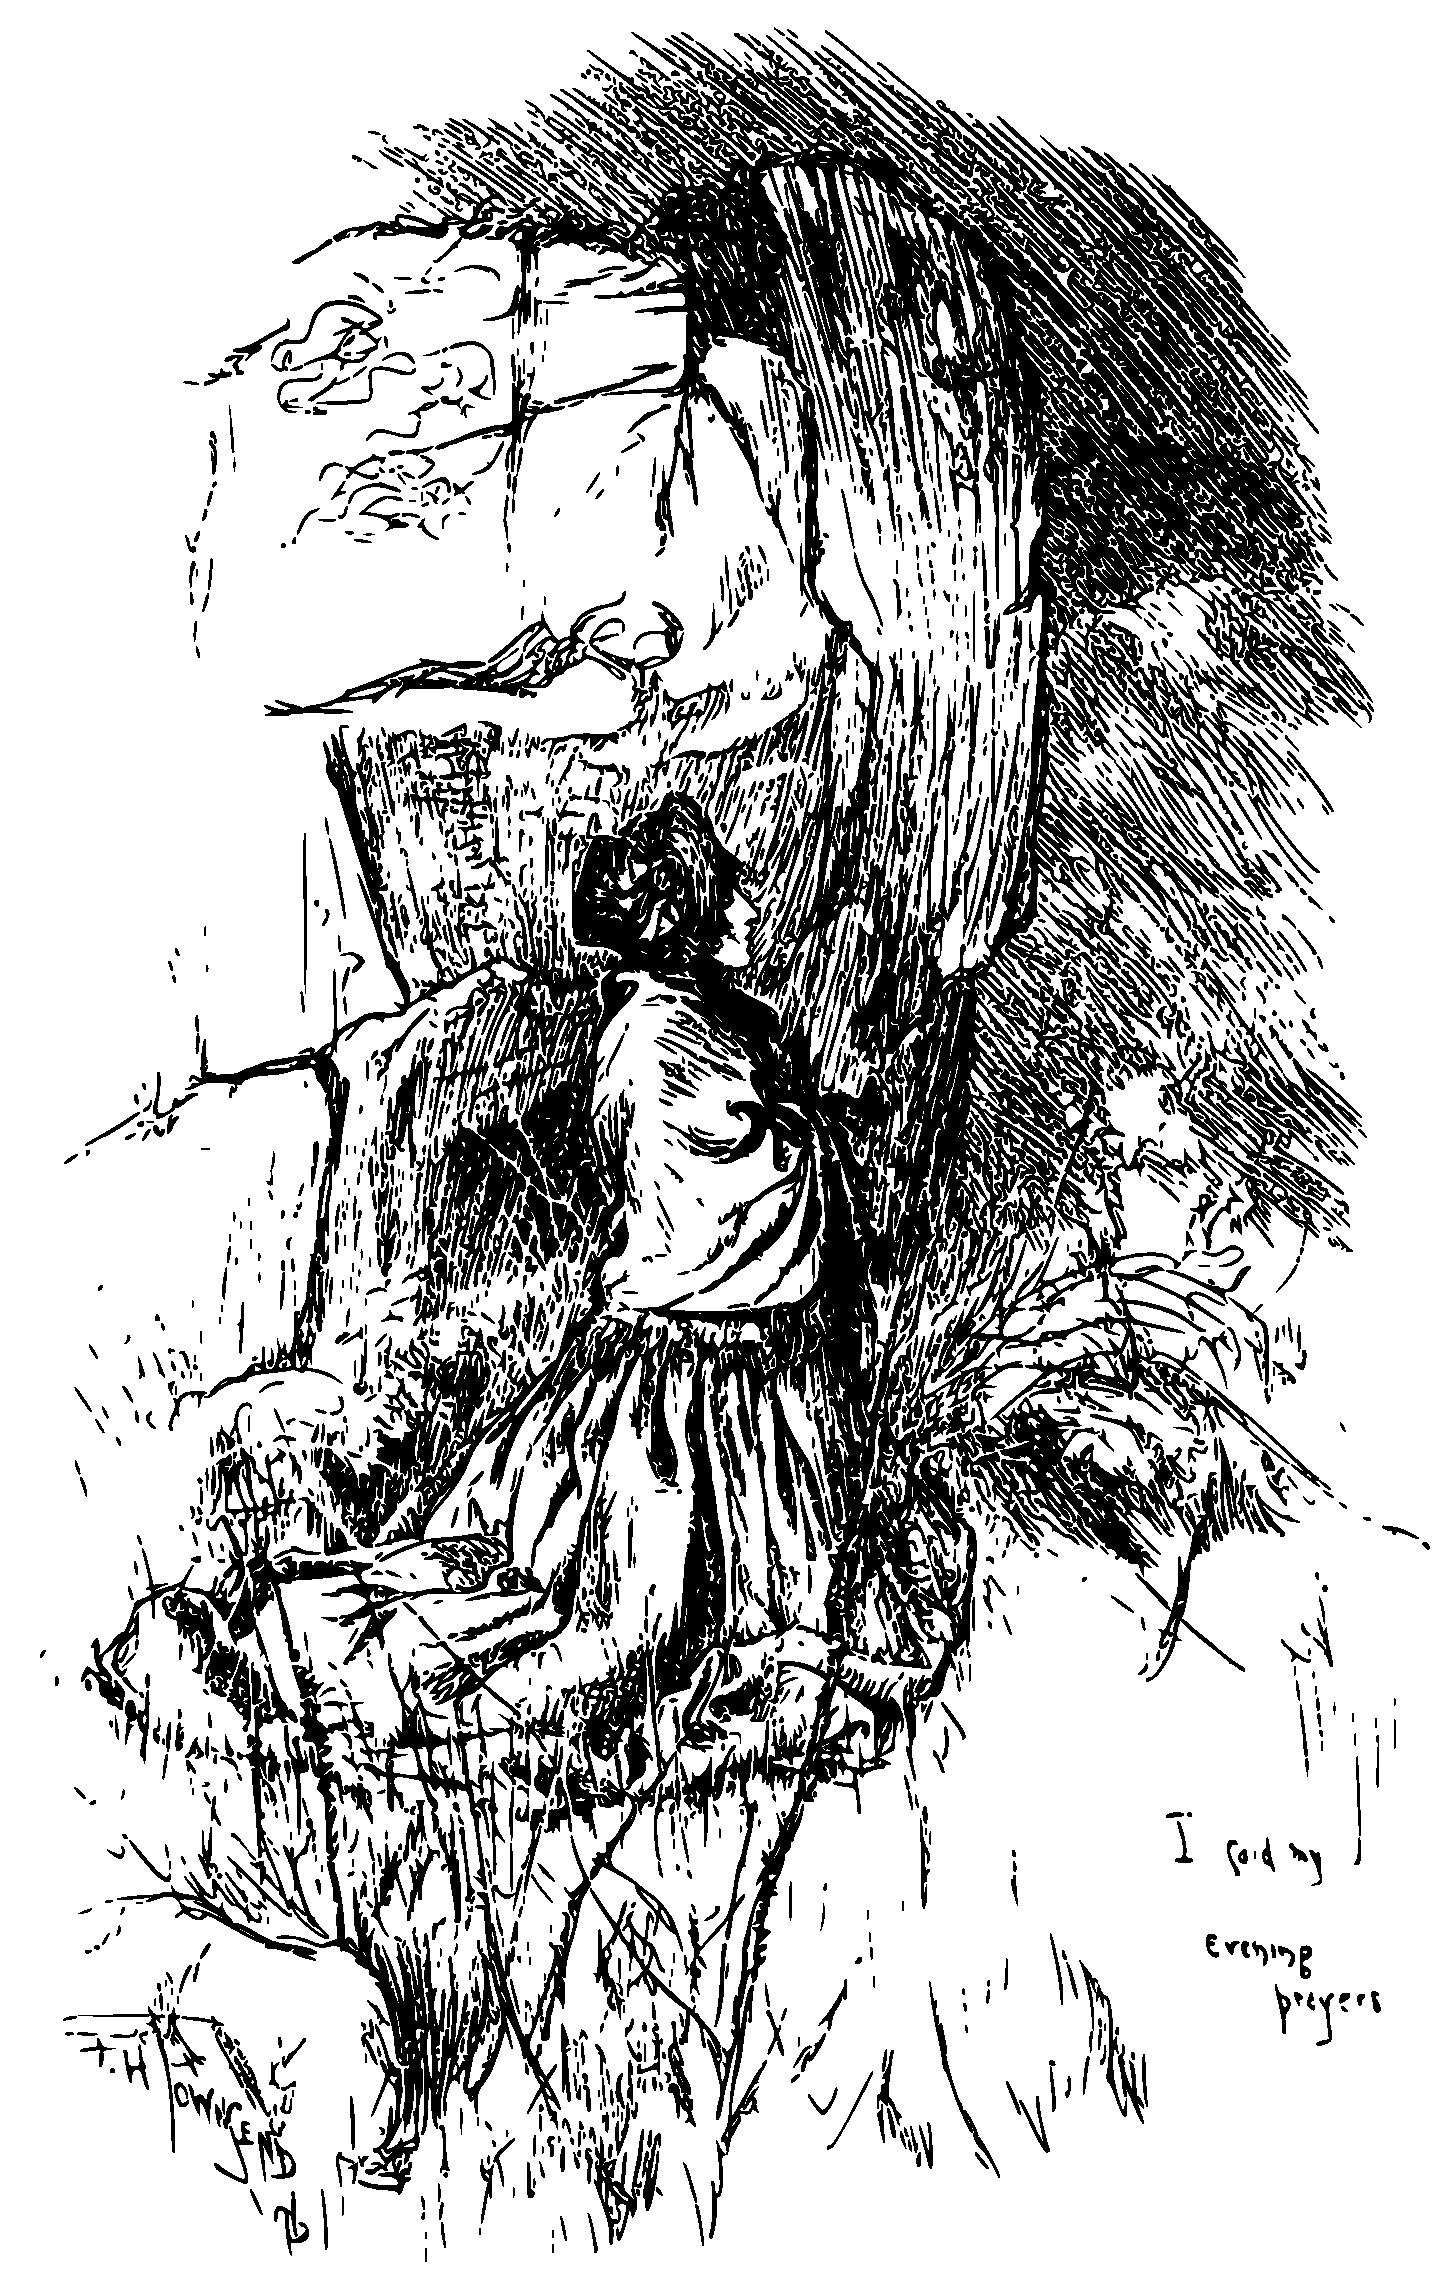
\includegraphics[width=\linewidth]{images/p311b.pdf}
	\end{sidecaption}
\end{figure}

Beside the crag the heath was very deep: when I lay down my feet were
buried in it; rising high on each side, it left only a narrow space for
the night-air to invade. I folded my shawl double, and spread it over
me for a coverlet; a low, mossy swell was my pillow. Thus lodged, I was
not, at least---at the commencement of the night, cold.

My rest might have been blissful enough, only a sad heart broke it. It
plained of its gaping wounds, its inward bleeding, its riven chords. It
trembled for \Mr{} Rochester and his doom; it bemoaned him with bitter
pity; it demanded him with ceaseless longing; and, impotent as a bird
with both wings broken, it still quivered its shattered pinions in vain
attempts to seek him.

Worn out with this torture of thought, I rose to my knees. Night was
come, and her planets were risen: a safe, still night: too serene for
the companionship of fear. We know that God is everywhere; but
certainly we feel His presence most when His works are on the grandest
scale spread before us; and it is in the unclouded night-sky, where His
worlds wheel their silent course, that we read clearest His infinitude,
His omnipotence, His omnipresence. I had risen to my knees to pray for
\Mr{} Rochester. Looking up, I, with tear-dimmed eyes, saw the mighty
Milky-way. Remembering what it was---what countless systems there swept
space like a soft trace of light---I felt the might and strength of
God. Sure was I of His efficiency to save what He had made: convinced I
grew that neither earth should perish, nor one of the souls it
treasured. I turned my prayer to thanksgiving: the Source of Life was
also the Saviour of spirits. \Mr{} Rochester was safe; he was God's, and
by God would he be guarded. I again nestled to the breast of the hill;
and ere long in sleep forgot sorrow.

But next day, Want came to me pale and bare. Long after the little
birds had left their nests; long after bees had come in the sweet prime
of day to gather the heath honey before the dew was dried---when the
long morning shadows were curtailed, and the sun filled earth and
sky---I got up, and I looked round me.

What a still, hot, perfect day! What a golden desert this spreading
moor! Everywhere sunshine. I wished I could live in it and on it. I
saw a lizard run over the crag; I saw a bee busy among the sweet
bilberries. I would fain at the moment have become bee or lizard, that
I might have found fitting nutriment, permanent shelter here. But I was
a human being, and had a human being's wants: I must not linger where
there was nothing to supply them. I rose; I looked back at the bed I
had left. Hopeless of the future, I wished but this---that my Maker had
that night thought good to require my soul of me while I slept; and that
this weary frame, absolved by death from further conflict with fate, had
now but to decay quietly, and mingle in peace with the soil of this
wilderness. Life, however, was yet in my possession, with all its
requirements, and pains, and responsibilities. The burden must be
carried; the want provided for; the suffering endured; the
responsibility fulfilled. I set out.

Whitcross regained, I followed a road which led from the sun, now
fervent and high. By no other circumstance had I will to decide my
choice. I walked a long time, and when I thought I had nearly done
enough, and might conscientiously yield to the fatigue that almost
overpowered me---might relax this forced action, and, sitting down on a
stone I saw near, submit resistlessly to the apathy that clogged heart
and limb---I heard a bell chime---a church bell.

I turned in the direction of the sound, and there, amongst the romantic
hills, whose changes and aspect I had ceased to note an hour ago, I saw
a hamlet and a spire. All the valley at my right hand was full of
pasture-fields, and cornfields, and wood; and a glittering stream ran
zig-zag through the varied shades of green, the mellowing grain, the
sombre woodland, the clear and sunny lea. Recalled by the rumbling of
wheels to the road before me, I saw a heavily-laden waggon labouring up
the hill, and not far beyond were two cows and their drover. Human life
and human labour were near. I must struggle on: strive to live and bend
to toil like the rest.

About two o'clock \PM{} I entered the village. At the bottom of its one
street there was a little shop with some cakes of bread in the window.
I coveted a cake of bread. With that refreshment I could perhaps regain
a degree of energy: without it, it would be difficult to proceed. The
wish to have some strength and some vigour returned to me as soon as I
was amongst my fellow-beings. I felt it would be degrading to faint
with hunger on the causeway of a hamlet. Had I nothing about me I could
offer in exchange for one of these rolls? I considered. I had a small
silk handkerchief tied round my throat; I had my gloves. I could hardly
tell how men and women in extremities of destitution proceeded. I did
not know whether either of these articles would be accepted: probably
they would not; but I must try.

I entered the shop: a woman was there. Seeing a respectably-dressed
person, a lady as she supposed, she came forward with civility. How
could she serve me? I was seized with shame: my tongue would not utter
the request I had prepared. I dared not offer her the half-worn gloves,
the creased handkerchief: besides, I felt it would be absurd. I only
begged permission to sit down a moment, as I was tired. Disappointed in
the expectation of a customer, she coolly acceded to my request. She
pointed to a seat; I sank into it. I felt sorely urged to weep; but
conscious how unseasonable such a manifestation would be, I restrained
it. Soon I asked her \enquote{if there were any dressmaker or
	plain-workwoman in the village?}

\enquote{Yes; two or three. Quite as many as there was employment for.}

I reflected. I was driven to the point now. I was brought face to face
with Necessity. I stood in the position of one without a resource,
without a friend, without a coin. I must do something. What? I must
apply somewhere. Where?

\enquote{Did she know of any place in the neighbourhood where a servant
	was wanted?}

\enquote{Nay; she couldn't say.}

\enquote{What was the chief trade in this place? What did most of the
	people do?}

\enquote{Some were farm labourers; a good deal worked at \Mr{} Oliver's
	needle-factory, and at the foundry.}

\enquote{Did \Mr{} Oliver employ women?}

\enquote{Nay; it was men's work.}

\enquote{And what do the women do?}

\enquote{I knawn't,} was the answer. \enquote{Some does one thing, and
	some another. Poor folk mun get on as they can.}

She seemed to be tired of my questions: and, indeed, what claim had I to
importune her? A neighbour or two came in; my chair was evidently
wanted. I took leave.

I passed up the street, looking as I went at all the houses to the right
hand and to the left; but I could discover no pretext, nor see an
inducement to enter any. I rambled round the hamlet, going sometimes to
a little distance and returning again, for an hour or more. Much
exhausted, and suffering greatly now for want of food, I turned aside
into a lane and sat down under the hedge. Ere many minutes had elapsed,
I was again on my feet, however, and again searching something---a
resource, or at least an informant. A pretty little house stood at the
top of the lane, with a garden before it, exquisitely neat and
brilliantly blooming. I stopped at it. What business had I to approach
the white door or touch the glittering knocker? In what way could it
possibly be the interest of the inhabitants of that dwelling to serve
me? Yet I drew near and knocked. A mild-looking, cleanly-attired young
woman opened the door. In such a voice as might be expected from a
hopeless heart and fainting frame---a voice wretchedly low and
faltering---I asked if a servant was wanted here?

\enquote{No,} said she; \enquote{we do not keep a servant.}

\enquote{Can you tell me where I could get employment of any kind?} I
continued. \enquote{I am a stranger, without acquaintance in this
	place. I want some work: no matter what.}

But it was not her business to think for me, or to seek a place for me:
besides, in her eyes, how doubtful must have appeared my character,
position, tale. She shook her head, she \enquote{was sorry she could
	give me no information,} and the white door closed, quite gently and
civilly: but it shut me out. If she had held it open a little longer, I
believe I should have begged a piece of bread; for I was now brought
low.

I could not bear to return to the sordid village, where, besides, no
prospect of aid was visible. I should have longed rather to deviate to
a wood I saw not far off, which appeared in its thick shade to offer
inviting shelter; but I was so sick, so weak, so gnawed with nature's
cravings, instinct kept me roaming round abodes where there was a chance
of food. Solitude would be no solitude---rest no rest---while the
vulture, hunger, thus sank beak and talons in my side.

I drew near houses; I left them, and came back again, and again I
wandered away: always repelled by the consciousness of having no claim
to ask---no right to expect interest in my isolated lot. Meantime, the
afternoon advanced, while I thus wandered about like a lost and starving
dog. In crossing a field, I saw the church spire before me: I hastened
towards it. Near the churchyard, and in the middle of a garden, stood a
well-built though small house, which I had no doubt was the parsonage.
I remembered that strangers who arrive at a place where they have no
friends, and who want employment, sometimes apply to the clergyman for
introduction and aid. It is the clergyman's function to help---at least
with advice---those who wished to help themselves. I seemed to have
something like a right to seek counsel here. Renewing then my courage,
and gathering my feeble remains of strength, I pushed on. I reached the
house, and knocked at the kitchen-door. An old woman opened: I asked
was this the parsonage?

\enquote{Yes.}

\enquote{Was the clergyman in?}

\enquote{No.}

\enquote{Would he be in soon?}

\enquote{No, he was gone from home.}

\enquote{To a distance?}

\enquote{Not so far---happen three mile. He had been called away by the
	sudden death of his father: he was at Marsh End now, and would very
	likely stay there a fortnight longer.}

\enquote{Was there any lady of the house?}

\enquote{Nay, there was naught but her, and she was housekeeper;} and of
her, reader, I could not bear to ask the relief for want of which I was
sinking; I could not yet beg; and again I crawled away.

Once more I took off my handkerchief---once more I thought of the cakes
of bread in the little shop. Oh, for but a crust! for but one mouthful
to allay the pang of famine! Instinctively I turned my face again to
the village; I found the shop again, and I went in; and though others
were there besides the woman I ventured the request---\enquote{Would she
	give me a roll for this handkerchief?}

She looked at me with evident suspicion: \enquote{Nay, she never sold
	stuff i' that way.}

Almost desperate, I asked for half a cake; she again refused.
\enquote{How could she tell where I had got the handkerchief?} she said.

\enquote{Would she take my gloves?}

\enquote{No! what could she do with them?}

Reader, it is not pleasant to dwell on these details. Some say there is
enjoyment in looking back to painful experience past; but at this day I
can scarcely bear to review the times to which I allude: the moral
degradation, blent with the physical suffering, form too distressing a
recollection ever to be willingly dwelt on. I blamed none of those who
repulsed me. I felt it was what was to be expected, and what could not
be helped: an ordinary beggar is frequently an object of suspicion; a
well-dressed beggar inevitably so. To be sure, what I begged was
employment; but whose business was it to provide me with employment?
Not, certainly, that of persons who saw me then for the first time, and
who knew nothing about my character. And as to the woman who would not
take my handkerchief in exchange for her bread, why, she was right, if
the offer appeared to her sinister or the exchange unprofitable. Let me
condense now. I am sick of the subject.

A little before dark I passed a farm-house, at the open door of which
the farmer was sitting, eating his supper of bread and cheese. I
stopped and said---

\enquote{Will you give me a piece of bread? for I am very hungry.} He
cast on me a glance of surprise; but without answering, he cut a thick
slice from his loaf, and gave it to me. I imagine he did not think I
was a beggar, but only an eccentric sort of lady, who had taken a fancy
to his brown loaf. As soon as I was out of sight of his house, I sat
down and ate it.

I could not hope to get a lodging under a roof, and sought it in the
wood I have before alluded to. But my night was wretched, my rest
broken: the ground was damp, the air cold: besides, intruders passed
near me more than once, and I had again and again to change my quarters;
no sense of safety or tranquillity befriended me. Towards morning it
rained; the whole of the following day was wet. Do not ask me, reader,
to give a minute account of that day; as before, I sought work; as
before, I was repulsed; as before, I starved; but once did food pass my
lips. At the door of a cottage I saw a little girl about to throw a
mess of cold porridge into a pig trough. \enquote{Will you give me
	that?} I asked.

\begin{figure}
	\begin{sidecaption}{\enquote{Will you give me that?}\linebreak I asked.}[p316b]
		\centering
		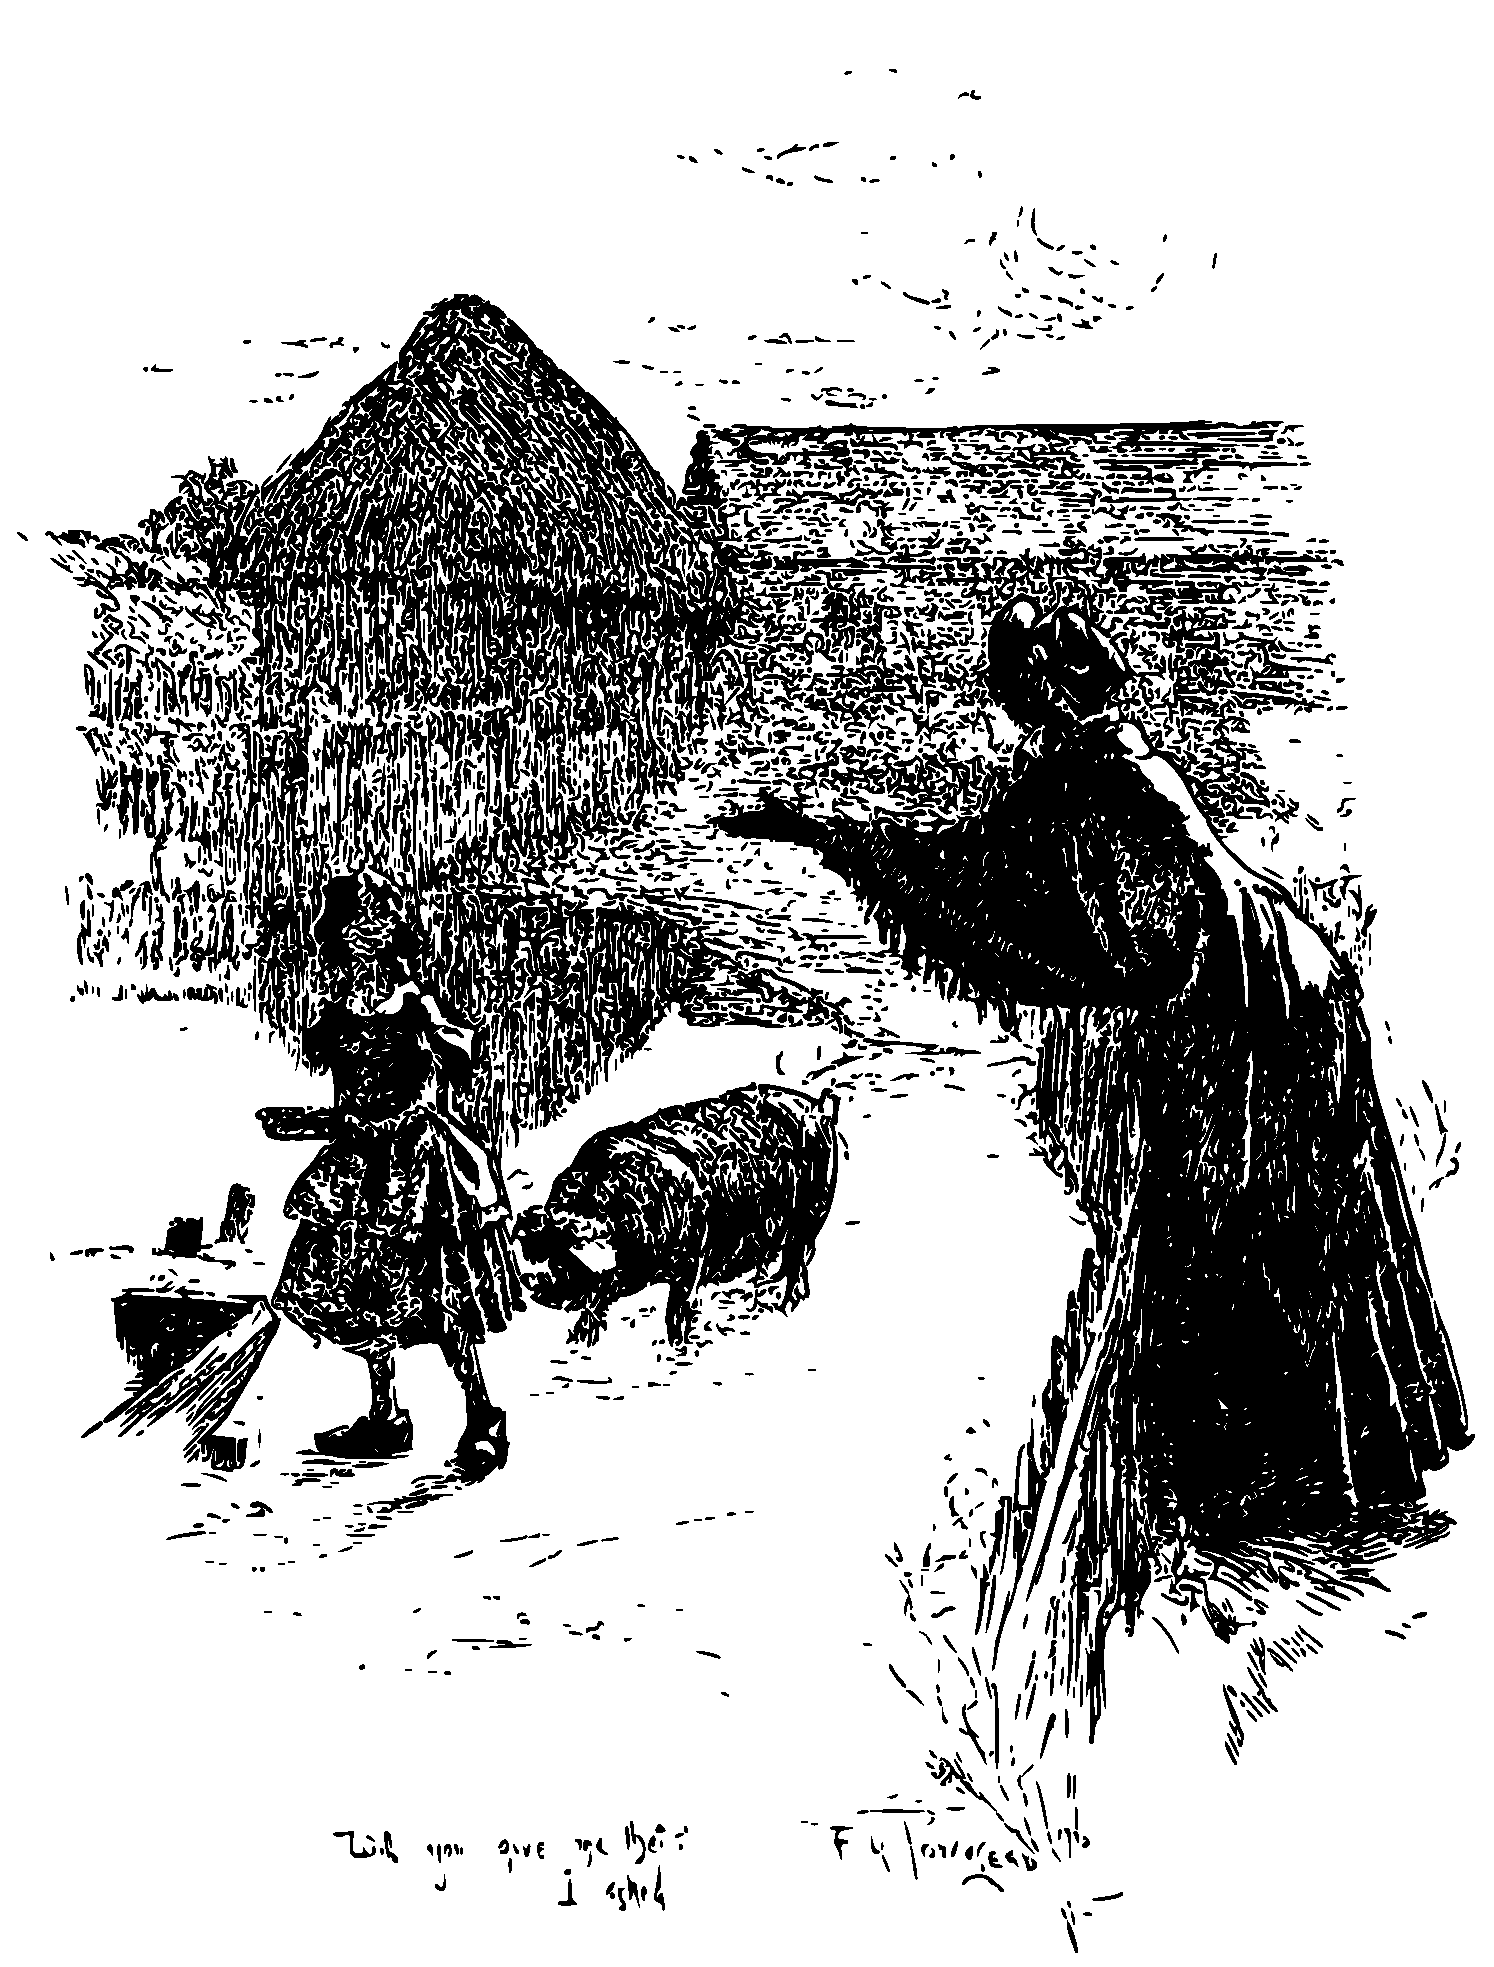
\includegraphics[width=\linewidth]{images/p316b.pdf}
	\end{sidecaption}
\end{figure}

She stared at me. \enquote{Mother!} she exclaimed, \enquote{there is a
	woman wants me to give her these porridge.}

\enquote{Well lass,} replied a voice within, \enquote{give it her if
	she's a beggar. T' pig doesn't want it.}

The girl emptied the stiffened mould into my hand, and I devoured it
ravenously.

As the wet twilight deepened, I stopped in a solitary bridle-path, which
I had been pursuing an hour or more.

\enquote{My strength is quite failing me,} I said in a soliloquy.
\enquote{I feel I cannot go much farther. Shall I be an outcast again
	this night? While the rain descends so, must I lay my head on the cold,
	drenched ground? I fear I cannot do otherwise: for who will receive
	me? But it will be very dreadful, with this feeling of hunger,
	faintness, chill, and this sense of desolation---this total prostration
	of hope. In all likelihood, though, I should die before morning. And
	why cannot I reconcile myself to the prospect of death? Why do I
	struggle to retain a valueless life? Because I know, or believe, \Mr{}
	Rochester is living: and then, to die of want and cold is a fate to
	which nature cannot submit passively. Oh, Providence! sustain me a
	little longer! Aid!---direct me!}

My glazed eye wandered over the dim and misty landscape. I saw I had
strayed far from the village: it was quite out of sight. The very
cultivation surrounding it had disappeared. I had, by cross-ways and
by-paths, once more drawn near the tract of moorland; and now, only a
few fields, almost as wild and unproductive as the heath from which they
were scarcely reclaimed, lay between me and the dusky hill.

\enquote{Well, I would rather die yonder than in a street or on a
	frequented road,} I reflected. \enquote{And far better that crows and
	ravens---if any ravens there be in these regions---should pick my flesh
	from my bones, than that they should be prisoned in a workhouse coffin
	and moulder in a pauper's grave.}

To the hill, then, I turned. I reached it. It remained now only to
find a hollow where I could lie down, and feel at least hidden, if not
secure. But all the surface of the waste looked level. It showed no
variation but of tint: green, where rush and moss overgrew the marshes;
black, where the dry soil bore only heath. Dark as it was getting, I
could still see these changes, though but as mere alternations of light
and shade; for colour had faded with the daylight.

My eye still roved over the sullen swell and along the moor-edge,
vanishing amidst the wildest scenery, when at one dim point, far in
among the marshes and the ridges, a light sprang up. \enquote{That is an
	\emph{ignis fatuus},} was my first thought; and I expected it would
soon vanish. It burnt on, however, quite steadily, neither receding nor
advancing. \enquote{Is it, then, a bonfire just kindled?} I
questioned. I watched to see whether it would spread: but no; as it did
not diminish, so it did not enlarge. \enquote{It may be a candle in a
	house,} I then conjectured; \enquote{but if so, I can never reach it.
	It is much too far away: and were it within a yard of me, what would it
	avail? I should but knock at the door to have it shut in my face.}

And I sank down where I stood, and hid my face against the ground. I
lay still a while: the night-wind swept over the hill and over me, and
died moaning in the distance; the rain fell fast, wetting me afresh to
the skin. Could I but have stiffened to the still frost---the friendly
numbness of death---it might have pelted on; I should not have felt it;
but my yet living flesh shuddered at its chilling influence. I rose ere
long.

The light was yet there, shining dim but constant through the rain. I
tried to walk again: I dragged my exhausted limbs slowly towards it. It
led me aslant over the hill, through a wide bog, which would have been
impassable in winter, and was splashy and shaking even now, in the
height of summer. Here I fell twice; but as often I rose and rallied my
faculties. This light was my forlorn hope: I must gain it.

Having crossed the marsh, I saw a trace of white over the moor. I
approached it; it was a road or a track: it led straight up to the
light, which now beamed from a sort of knoll, amidst a clump of
trees---firs, apparently, from what I could distinguish of the character
of their forms and foliage through the gloom. My star vanished as I
drew near: some obstacle had intervened between me and it. I put out my
hand to feel the dark mass before me: I discriminated the rough stones
of a low wall---above it, something like palisades, and within, a high
and prickly hedge. I groped on. Again a whitish object gleamed before
me: it was a gate---a wicket; it moved on its hinges as I touched it.
On each side stood a sable bush-holly or yew.

Entering the gate and passing the shrubs, the silhouette of a house rose
to view, black, low, and rather long; but the guiding light shone
nowhere. All was obscurity. Were the inmates retired to rest? I
feared it must be so. In seeking the door, I turned an angle: there
shot out the friendly gleam again, from the lozenged panes of a very
small latticed window, within a foot of the ground, made still smaller
by the growth of ivy or some other creeping plant, whose leaves
clustered thick over the portion of the house wall in which it was set.
The aperture was so screened and narrow, that curtain or shutter had
been deemed unnecessary; and when I stooped down and put aside the spray
of foliage shooting over it, I could see all within. I could see
clearly a room with a sanded floor, clean scoured; a dresser of walnut,
with pewter plates ranged in rows, reflecting the redness and radiance
of a glowing peat-fire. I could see a clock, a white deal table, some
chairs. The candle, whose ray had been my beacon, burnt on the table;
and by its light an elderly woman, somewhat rough-looking, but
scrupulously clean, like all about her, was knitting a stocking.

I noticed these objects cursorily only---in them there was nothing
extraordinary. A group of more interest appeared near the hearth,
sitting still amidst the rosy peace and warmth suffusing it. Two young,
graceful women---ladies in every point---sat, one in a low
rocking-chair, the other on a lower stool; both wore deep mourning of
crape and bombazeen, which sombre garb singularly set off very fair
necks and faces: a large old pointer dog rested its massive head on the
knee of one girl---in the lap of the other was cushioned a black cat.

A strange place was this humble kitchen for such occupants! Who were
they? They could not be the daughters of the elderly person at the
table; for she looked like a rustic, and they were all delicacy and
cultivation. I had nowhere seen such faces as theirs: and yet, as I
gazed on them, I seemed intimate with every lineament. I cannot call
them handsome---they were too pale and grave for the word: as they each
bent over a book, they looked thoughtful almost to severity. A stand
between them supported a second candle and two great volumes, to which
they frequently referred, comparing them, seemingly, with the smaller
books they held in their hands, like people consulting a dictionary to
aid them in the task of translation. This scene was as silent as if all
the figures had been shadows and the firelit apartment a picture: so
hushed was it, I could hear the cinders fall from the grate, the clock
tick in its obscure corner; and I even fancied I could distinguish the
click-click of the woman's knitting-needles. When, therefore, a voice
broke the strange stillness at last, it was audible enough to me.

\enquote{Listen, Diana,} said one of the absorbed students;
\enquote{Franz and old Daniel are together in the night-time, and Franz
	is telling a dream from which he has awakened in terror---listen!} And
in a low voice she read something, of which not one word was
intelligible to me; for it was in an unknown tongue---neither French nor
Latin. Whether it were Greek or German I could not tell.

\enquote{That is strong,} she said, when she had finished: \enquote{I
	relish it.} The other girl, who had lifted her head to listen to her
sister, repeated, while she gazed at the fire, a line of what had been
read. At a later day, I knew the language and the book; therefore, I
will here quote the line: though, when I first heard it, it was only
like a stroke on sounding brass to me---conveying no meaning:---

\enquote{\foreignquote{german}{Da trat hervor Einer, anzusehen wie die Sternen
		Nacht.}\footnote{\enquote{Then one stepped forth, who appeared like the stars of the night.}}
	Good! good!} she exclaimed, while her dark and deep eye
sparkled. \enquote{There you have a dim and mighty archangel fitly set
	before you! The line is worth a hundred pages of fustian.
	\foreignquote{german}{Ich wäge die Gedanken in der Schale meines Zornes und die
		Werke mit dem Gewichte meines Grimms.}\footnote{
		\enquote{I weigh thoughts in the scale of my anger and works against the weight of my wrath.}} I like it!}

Both were again silent.

\enquote{Is there ony country where they talk i' that way?} asked the
old woman, looking up from her knitting.

\enquote{Yes, Hannah---a far larger country than England, where they
	talk in no other way.}

\enquote{Well, for sure case, I knawn't how they can understand t' one
	t'other: and if either o' ye went there, ye could tell what they said, I
	guess?}

\enquote{We could probably tell something of what they said, but not
	all---for we are not as clever as you think us, Hannah. We don't speak
	German, and we cannot read it without a dictionary to help us.}

\enquote{And what good does it do you?}

\enquote{We mean to teach it some time---or at least the elements, as
	they say; and then we shall get more money than we do now.}

\enquote{Varry like: but give ower studying; ye've done enough for
	to-night.}

\enquote{I think we have: at least I'm tired. Mary, are you?}

\enquote{Mortally: after all, it's tough work fagging away at a language
	with no master but a lexicon.}

\enquote{It is, especially such a language as this crabbed but glorious
	Deutsch. I wonder when \St{} John will come home.}

\enquote{Surely he will not be long now: it is just ten (looking at a
	little gold watch she drew from her girdle). It rains fast, Hannah:
	will you have the goodness to look at the fire in the parlour?}

The woman rose: she opened a door, through which I dimly saw a passage:
soon I heard her stir a fire in an inner room; she presently came back.

\enquote{Ah, childer!} said she, \enquote{it fair troubles me to go into
	yond' room now: it looks so lonesome wi' the chair empty and set back in
	a corner.}

She wiped her eyes with her apron: the two girls, grave before, looked
sad now.

\enquote{But he is in a better place,} continued Hannah: \enquote{we
	shouldn't wish him here again. And then, nobody need to have a quieter
	death nor he had.}

\enquote{You say he never mentioned us?} inquired one of the ladies.

\enquote{He hadn't time, bairn: he was gone in a minute, was your
	father. He had been a bit ailing like the day before, but naught to
	signify; and when \Mr{} \St{} John asked if he would like either o' ye to be
	sent for, he fair laughed at him. He began again with a bit of a
	heaviness in his head the next day---that is, a fortnight sin'---and he
	went to sleep and niver wakened: he wor a'most stark when your brother
	went into t' chamber and fand him. Ah, childer! that's t' last o' t'
	old stock---for ye and \Mr{} \St{} John is like of different soart to them
	\enquote{at's gone; for all your mother wor mich i} your way, and
	a'most as book-learned. She wor the pictur' o' ye, Mary: Diana is more
	like your father.}

I thought them so similar I could not tell where the old servant (for
such I now concluded her to be) saw the difference. Both were fair
complexioned and slenderly made; both possessed faces full of
distinction and intelligence. One, to be sure, had hair a shade darker
than the other, and there was a difference in their style of wearing it;
Mary's pale brown locks were parted and braided smooth: Diana's duskier
tresses covered her neck with thick curls. The clock struck ten.

\enquote{Ye'll want your supper, I am sure,} observed Hannah;
\enquote{and so will \Mr{} \St{} John when he comes in.}

And she proceeded to prepare the meal. The ladies rose; they seemed
about to withdraw to the parlour. Till this moment, I had been so
intent on watching them, their appearance and conversation had excited
in me so keen an interest, I had half-forgotten my own wretched
position: now it recurred to me. More desolate, more desperate than
ever, it seemed from contrast. And how impossible did it appear to
touch the inmates of this house with concern on my behalf; to make them
believe in the truth of my wants and woes---to induce them to vouchsafe
a rest for my wanderings! As I groped out the door, and knocked at it
hesitatingly, I felt that last idea to be a mere chimera. Hannah
opened.

\enquote{What do you want?} she inquired, in a voice of surprise, as she
surveyed me by the light of the candle she held.

\enquote{May I speak to your mistresses?} I said.

\enquote{You had better tell me what you have to say to them. Where do
	you come from?}

\enquote{I am a stranger.}

\enquote{What is your business here at this hour?}

\enquote{I want a night's shelter in an out-house or anywhere, and a
	morsel of bread to eat.}

Distrust, the very feeling I dreaded, appeared in Hannah's face.
\enquote{I'll give you a piece of bread,} she said, after a pause;
\enquote{but we can't take in a vagrant to lodge. It isn't likely.}

\enquote{Do let me speak to your mistresses.}

\enquote{No, not I\@. What can they do for you? You should not be roving
	about now; it looks very ill.}

\enquote{But where shall I go if you drive me away? What shall I do?}

\enquote{Oh, I'll warrant you know where to go and what to do. Mind you
	don't do wrong, that's all. Here is a penny; now go---}

\enquote{A penny cannot feed me, and I have no strength to go farther.
	Don't shut the door:---oh, don't, for God's sake!}

\enquote{I must; the rain is driving in---}

\enquote{Tell the young ladies. Let me see them---}

\enquote{Indeed, I will not. You are not what you ought to be, or you
	wouldn't make such a noise. Move off.}

\enquote{But I must die if I am turned away.}

\enquote{Not you. I'm fear'd you have some ill plans agate, that bring
	you about folk's houses at this time o' night. If you've any
	followers---housebreakers or such like---anywhere near, you may tell
	them we are not by ourselves in the house; we have a gentleman, and
	dogs, and guns.} Here the honest but inflexible servant clapped the
door to and bolted it within.

This was the climax. A pang of exquisite suffering---a throe of true
despair---rent and heaved my heart. Worn out, indeed, I was; not
another step could I stir. I sank on the wet doorstep: I groaned---I
wrung my hands---I wept in utter anguish. Oh, this spectre of death!
Oh, this last hour, approaching in such horror! Alas, this
isolation---this banishment from my kind! Not only the anchor of hope,
but the footing of fortitude was gone---at least for a moment; but the
last I soon endeavoured to regain.

\enquote{I can but die,} I said, \enquote{and I believe in God. Let me
	try to wait His will in silence.}

These words I not only thought, but uttered; and thrusting back all my
misery into my heart, I made an effort to compel it to remain
there---dumb and still.

\enquote{All men must die,} said a voice quite close at hand;
\enquote{but all are not condemned to meet a lingering and premature
	doom, such as yours would be if you perished here of want.}

\enquote{Who or what speaks?} I asked, terrified at the unexpected
sound, and incapable now of deriving from any occurrence a hope of aid.
A form was near---what form, the pitch-dark night and my enfeebled
vision prevented me from distinguishing. With a loud long knock, the
new-comer appealed to the door.

\enquote{Is it you, \Mr{} \St{} John?} cried Hannah.

\enquote{Yes---yes; open quickly.}

\enquote{Well, how wet and cold you must be, such a wild night as it
	is! Come in---your sisters are quite uneasy about you, and I believe
	there are bad folks about. There has been a beggar-woman---I declare
	she is not gone yet!---laid down there. Get up! for shame! Move off, I
	say!}

\enquote{Hush, Hannah! I have a word to say to the woman. You have
	done your duty in excluding, now let me do mine in admitting her. I was
	near, and listened to both you and her. I think this is a peculiar
	case---I must at least examine into it. Young woman, rise, and pass
	before me into the house.}

\begin{figure}
	\begin{sidecaption}{\enquote{Hush, Hannah!\linebreak I have a word\linebreak to say to the woman.}}[p323b]
		\centering
		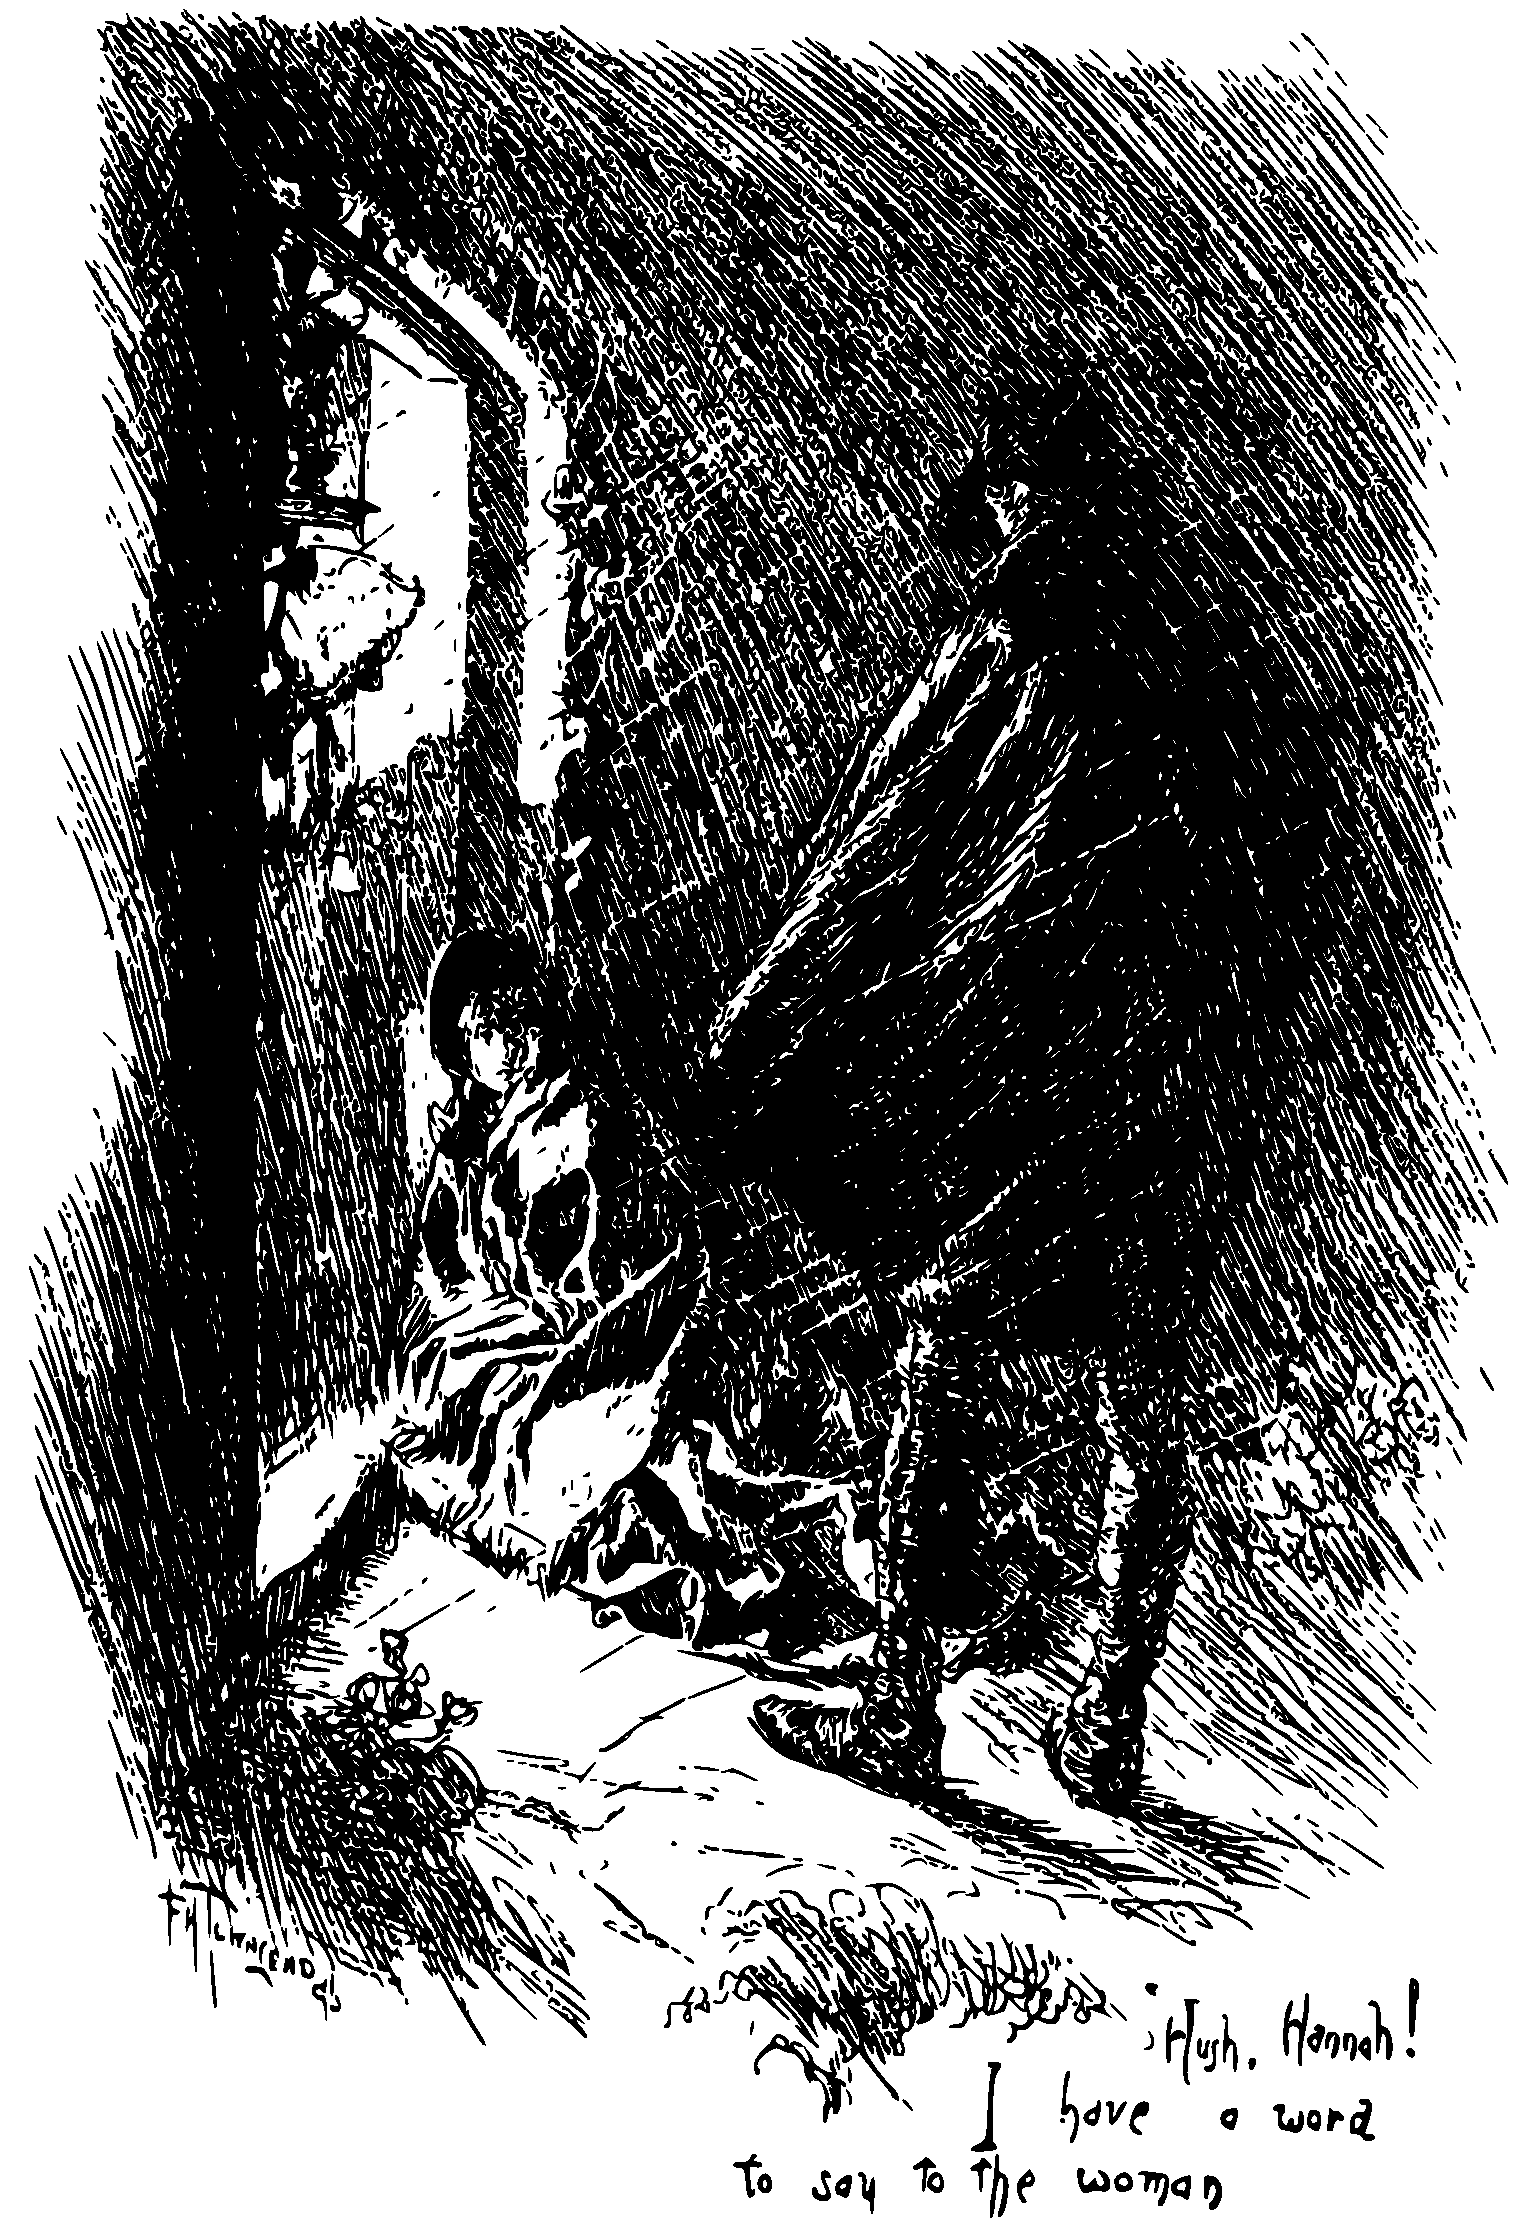
\includegraphics[width=\linewidth]{images/p323b.pdf}
	\end{sidecaption}
\end{figure}

With difficulty I obeyed him. Presently I stood within that clean,
bright kitchen---on the very hearth---trembling, sickening; conscious of
an aspect in the last degree ghastly, wild, and weather-beaten. The two
ladies, their brother, \Mr{} \St{} John, the old servant, were all gazing at
me.

\enquote{\St{} John, who is it?} I heard one ask.

\enquote{I cannot tell: I found her at the door,} was the reply.

\enquote{She does look white,} said Hannah.

\enquote{As white as clay or death,} was responded. \enquote{She will
	fall: let her sit.}

And indeed my head swam: I dropped, but a chair received me. I still
possessed my senses, though just now I could not speak.

\enquote{Perhaps a little water would restore her. Hannah, fetch some.
	But she is worn to nothing. How very thin, and how very bloodless!}

\enquote{A mere spectre!}

\enquote{Is she ill, or only famished?}

\enquote{Famished, I think. Hannah, is that milk? Give it me, and a
	piece of bread.}

Diana (I knew her by the long curls which I saw drooping between me and
the fire as she bent over me) broke some bread, dipped it in milk, and
put it to my lips. Her face was near mine: I saw there was pity in it,
and I felt sympathy in her hurried breathing. In her simple words, too,
the same balm-like emotion spoke: \enquote{Try to eat.}

\enquote{Yes---try,} repeated Mary gently; and Mary's hand removed my
sodden bonnet and lifted my head. I tasted what they offered me: feebly
at first, eagerly soon.

\enquote{Not too much at first---restrain her,} said the brother;
\enquote{she has had enough.} And he withdrew the cup of milk and the
plate of bread.

\enquote{A little more, \St{} John---look at the avidity in her eyes.}

\enquote{No more at present, sister. Try if she can speak now---ask her
	her name.}

I felt I could speak, and I answered---\enquote{My name is Jane
	Elliott.} Anxious as ever to avoid discovery, I had before resolved to
assume an \emph{alias}.

\enquote{And where do you live? Where are your friends?}

I was silent.

\enquote{Can we send for any one you know?}

I shook my head.

\enquote{What account can you give of yourself?}

Somehow, now that I had once crossed the threshold of this house, and
once was brought face to face with its owners, I felt no longer outcast,
vagrant, and disowned by the wide world. I dared to put off the
mendicant---to resume my natural manner and character. I began once
more to know myself; and when \Mr{} \St{} John demanded an account---which
at present I was far too weak to render---I said after a brief pause---

\enquote{Sir, I can give you no details to-night.}

\enquote{But what, then,} said he, \enquote{do you expect me to do for
	you?}

\enquote{Nothing,} I replied. My strength sufficed for but short
answers. Diana took the word---

\enquote{Do you mean,} she asked, \enquote{that we have now given you
	what aid you require? and that we may dismiss you to the moor and the
	rainy night?}

I looked at her. She had, I thought, a remarkable countenance, instinct
both with power and goodness. I took sudden courage. Answering her
compassionate gaze with a smile, I said---\enquote{I will trust you. If
	I were a masterless and stray dog, I know that you would not turn me
	from your hearth to-night: as it is, I really have no fear. Do with me
	and for me as you like; but excuse me from much discourse---my breath is
	short---I feel a spasm when I speak.} All three surveyed me, and all
three were silent.

\enquote{Hannah,} said \Mr{} \St{} John, at last, \enquote{let her sit there
	at present, and ask her no questions; in ten minutes more, give her the
	remainder of that milk and bread. Mary and Diana, let us go into the
	parlour and talk the matter over.}

They withdrew. Very soon one of the ladies returned---I could not tell
which. A kind of pleasant stupor was stealing over me as I sat by the
genial fire. In an undertone she gave some directions to Hannah. Ere
long, with the servant's aid, I contrived to mount a staircase; my
dripping clothes were removed; soon a warm, dry bed received me. I
thanked God---experienced amidst unutterable exhaustion a glow of
grateful joy---and slept.

\FChapter{Chapter Twenty-Nine}{29}

\Lettrine{T}{he} \textsc{recollection} of about three days and nights succeeding this is very
dim in my mind. I can recall some sensations felt in that interval; but
few thoughts framed, and no actions performed. I knew I was in a small
room and in a narrow bed. To that bed I seemed to have grown; I lay on
it motionless as a stone; and to have torn me from it would have been
almost to kill me. I took no note of the lapse of time---of the change
from morning to noon, from noon to evening. I observed when any one
entered or left the apartment: I could even tell who they were; I could
understand what was said when the speaker stood near to me; but I could
not answer; to open my lips or move my limbs was equally impossible.
Hannah, the servant, was my most frequent visitor. Her coming disturbed
me. I had a feeling that she wished me away: that she did not
understand me or my circumstances; that she was prejudiced against me.
Diana and Mary appeared in the chamber once or twice a day. They would
whisper sentences of this sort at my bedside---

\enquote{It is very well we took her in.}

\enquote{Yes; she would certainly have been found dead at the door in
	the morning had she been left out all night. I wonder what she has gone
	through?}

\enquote{Strange hardships, I imagine---poor, emaciated, pallid
	wanderer?}

\enquote{She is not an uneducated person, I should think, by her manner
	of speaking; her accent was quite pure; and the clothes she took off,
	though splashed and wet, were little worn and fine.}

\enquote{She has a peculiar face; fleshless and haggard as it is, I
	rather like it; and when in good health and animated, I can fancy her
	physiognomy would be agreeable.}

Never once in their dialogues did I hear a syllable of regret at the
hospitality they had extended to me, or of suspicion of, or aversion to,
myself. I was comforted.

\Mr{} \St{} John came but once: he looked at me, and said my state of
lethargy was the result of reaction from excessive and protracted
fatigue. He pronounced it needless to send for a doctor: nature, he was
sure, would manage best, left to herself. He said every nerve had been
overstrained in some way, and the whole system must sleep torpid a
while. There was no disease. He imagined my recovery would be rapid
enough when once commenced. These opinions he delivered in a few words,
in a quiet, low voice; and added, after a pause, in the tone of a man
little accustomed to expansive comment, \enquote{Rather an unusual
	physiognomy; certainly, not indicative of vulgarity or degradation.}

\enquote{Far otherwise,} responded Diana. \enquote{To speak truth, St.
	John, my heart rather warms to the poor little soul. I wish we may be
	able to benefit her permanently.}

\enquote{That is hardly likely,} was the reply. \enquote{You will find
	she is some young lady who has had a misunderstanding with her friends,
	and has probably injudiciously left them. We may, perhaps, succeed in
	restoring her to them, if she is not obstinate: but I trace lines of
	force in her face which make me sceptical of her tractability.} He
stood considering me some minutes; then added, \enquote{She looks
	sensible, but not at all handsome.}

\enquote{She is so ill, \St{} John.}

\enquote{Ill or well, she would always be plain. The grace and harmony
	of beauty are quite wanting in those features.}

On the third day I was better; on the fourth, I could speak, move, rise
in bed, and turn. Hannah had brought me some gruel and dry toast,
about, as I supposed, the dinner-hour. I had eaten with relish: the
food was good---void of the feverish flavour which had hitherto poisoned
what I had swallowed. When she left me, I felt comparatively strong and
revived: ere long satiety of repose and desire for action stirred me. I
wished to rise; but what could I put on? Only my damp and bemired
apparel; in which I had slept on the ground and fallen in the marsh. I
felt ashamed to appear before my benefactors so clad. I was spared the
humiliation.

On a chair by the bedside were all my own things, clean and dry. My
black silk frock hung against the wall. The traces of the bog were
removed from it; the creases left by the wet smoothed out: it was quite
decent. My very shoes and stockings were purified and rendered
presentable. There were the means of washing in the room, and a comb
and brush to smooth my hair. After a weary process, and resting every
five minutes, I succeeded in dressing myself. My clothes hung loose on
me; for I was much wasted, but I covered deficiencies with a shawl, and
once more, clean and respectable looking---no speck of the dirt, no
trace of the disorder I so hated, and which seemed so to degrade me,
left---I crept down a stone staircase with the aid of the banisters, to
a narrow low passage, and found my way presently to the kitchen.

It was full of the fragrance of new bread and the warmth of a generous
fire. Hannah was baking. Prejudices, it is well known, are most
difficult to eradicate from the heart whose soil has never been loosened
or fertilised by education: they grow there, firm as weeds among
stones. Hannah had been cold and stiff, indeed, at the first: latterly
she had begun to relent a little; and when she saw me come in tidy and
well-dressed, she even smiled.

\enquote{What, you have got up!} she said. \enquote{You are better,
	then. You may sit you down in my chair on the hearthstone, if you
	will.}

She pointed to the rocking-chair: I took it. She bustled about,
examining me every now and then with the corner of her eye. Turning to
me, as she took some loaves from the oven, she asked bluntly---

\enquote{Did you ever go a-begging afore you came here?}

I was indignant for a moment; but remembering that anger was out of the
question, and that I had indeed appeared as a beggar to her, I answered
quietly, but still not without a certain marked firmness---

\enquote{You are mistaken in supposing me a beggar. I am no beggar; any
	more than yourself or your young ladies.}

After a pause she said, \enquote{I dunnut understand that: you've like
	no house, nor no brass, I guess?}

\enquote{The want of house or brass (by which I suppose you mean money)
	does not make a beggar in your sense of the word.}

\enquote{Are you book-learned?} she inquired presently.

\enquote{Yes, very.}

\enquote{But you've never been to a boarding-school?}

\enquote{I was at a boarding-school eight years.}

She opened her eyes wide. \enquote{Whatever cannot ye keep yourself
	for, then?}

\enquote{I have kept myself; and, I trust, shall keep myself again.
	What are you going to do with these gooseberries?} I inquired, as she
brought out a basket of the fruit.

\enquote{Mak' 'em into pies.}

\enquote{Give them to me and I'll pick them.}

\enquote{Nay; I dunnut want ye to do nought.}

\enquote{But I must do something. Let me have them.}

She consented; and she even brought me a clean towel to spread over my
dress, \enquote{lest,} as she said, \enquote{I should mucky it.}

\enquote{Ye've not been used to sarvant's wark, I see by your hands,}
she remarked. \enquote{Happen ye've been a dressmaker?}

\enquote{No, you are wrong. And now, never mind what I have been: don't
	trouble your head further about me; but tell me the name of the house
	where we are.}

\enquote{Some calls it Marsh End, and some calls it Moor House.}

\enquote{And the gentleman who lives here is called \Mr{} \St{} John?}

\enquote{Nay; he doesn't live here: he is only staying a while. When he
	is at home, he is in his own parish at Morton.}

\enquote{That village a few miles off?} %fix missing end quote

\enquote{Aye.}

\enquote{And what is he?}

\enquote{He is a parson.}

I remembered the answer of the old housekeeper at the parsonage, when I
had asked to see the clergyman. \enquote{This, then, was his father's
	residence?}

\enquote{Aye; old \Mr{} Rivers lived here, and his father, and
	grandfather, and gurt (great) grandfather afore him.}

\enquote{The name, then, of that gentleman, is \Mr{} \St{} John Rivers?}

\enquote{Aye; \St{} John is like his kirstened name.}

\enquote{And his sisters are called Diana and Mary Rivers?}

\enquote{Yes.}

\enquote{Their father is dead?}

\enquote{Dead three weeks sin' of a stroke.}

\enquote{They have no mother?}

\enquote{The mistress has been dead this mony a year.}

\enquote{Have you lived with the family long?}

\enquote{I've lived here thirty year. I nursed them all three.}

\enquote{That proves you must have been an honest and faithful servant.
	I will say so much for you, though you have had the incivility to call
	me a beggar.}

She again regarded me with a surprised stare. \enquote{I believe,} she
said, \enquote{I was quite mista'en in my thoughts of you: but there is
	so mony cheats goes about, you mun forgie me.}

\enquote{And though,} I continued, rather severely, \enquote{you wished
	to turn me from the door, on a night when you should not have shut out a
	dog.}

\enquote{Well, it was hard: but what can a body do? I thought more o'
	th' childer nor of mysel: poor things! They've like nobody to tak' care
	on 'em but me. I'm like to look sharpish.}

I maintained a grave silence for some minutes.

\enquote{You munnut think too hardly of me,} she again remarked.

\enquote{But I do think hardly of you,} I said; \enquote{and I'll tell
	you why---not so much because you refused to give me shelter, or
	regarded me as an impostor, as because you just now made it a species of
	reproach that I had no \enquote{brass} and no house. Some of the best
	people that ever lived have been as destitute as I am; and if you are a
	Christian, you ought not to consider poverty a crime.}

\enquote{No more I ought,} said she: \enquote{\Mr{} \St{} John tells me so
	too; and I see I wor wrang---but I've clear a different notion on you
	now to what I had. You look a raight down dacent little crater.}

\enquote{That will do---I forgive you now. Shake hands.}

She put her floury and horny hand into mine; another and heartier smile
illumined her rough face, and from that moment we were friends.

Hannah was evidently fond of talking. While I picked the fruit, and she
made the paste for the pies, she proceeded to give me sundry details
about her deceased master and mistress, and \enquote{the childer,} as
she called the young people.

Old \Mr{} Rivers, she said, was a plain man enough, but a gentleman, and
of as ancient a family as could be found. Marsh End had belonged to the
Rivers ever since it was a house: and it was, she affirmed,
\enquote{aboon two hundred year old---for all it looked but a small,
	humble place, naught to compare wi' \Mr{} Oliver's grand hall down i'
	Morton Vale. But she could remember Bill Oliver's father a journeyman
	needlemaker; and th' Rivers wor gentry i' th' owd days o' th' Henrys, as
	onybody might see by looking into th' registers i' Morton Church
	vestry.} Still, she allowed, \enquote{the owd maister was like other
	folk---naught mich out o' t' common way: stark mad o' shooting, and
	farming, and sich like.} The mistress was different. She was a great
reader, and studied a deal; and the \enquote{bairns} had taken after
her. There was nothing like them in these parts, nor ever had been;
they had liked learning, all three, almost from the time they could
speak; and they had always been \enquote{of a mak' of their own.} \Mr{}
\St{} John, when he grew up, would go to college and be a parson; and the
girls, as soon as they left school, would seek places as governesses:
for they had told her their father had some years ago lost a great deal
of money by a man he had trusted turning bankrupt; and as he was now not
rich enough to give them fortunes, they must provide for themselves.
They had lived very little at home for a long while, and were only come
now to stay a few weeks on account of their father's death; but they did
so like Marsh End and Morton, and all these moors and hills about. They
had been in London, and many other grand towns; but they always said
there was no place like home; and then they were so agreeable with each
other---never fell out nor \enquote{threaped.} She did not know where
there was such a family for being united.

Having finished my task of gooseberry picking, I asked where the two
ladies and their brother were now.

\enquote{Gone over to Morton for a walk; but they would be back in
	half-an-hour to tea.}

They returned within the time Hannah had allotted them: they entered by
the kitchen door. \Mr{} \St{} John, when he saw me, merely bowed and passed
through; the two ladies stopped: Mary, in a few words, kindly and calmly
expressed the pleasure she felt in seeing me well enough to be able to
come down; Diana took my hand: she shook her head at me.

\enquote{You should have waited for my leave to descend,} she said.
\enquote{You still look very pale---and so thin! Poor child!---poor
	girl!}

Diana had a voice toned, to my ear, like the cooing of a dove. She
possessed eyes whose gaze I delighted to encounter. Her whole face
seemed to me full of charm. Mary's countenance was equally
intelligent---her features equally pretty; but her expression was more
reserved, and her manners, though gentle, more distant. Diana looked
and spoke with a certain authority: she had a will, evidently. It was
my nature to feel pleasure in yielding to an authority supported like
hers, and to bend, where my conscience and self-respect permitted, to an
active will.

\enquote{And what business have you here?} she continued. \enquote{It
	is not your place. Mary and I sit in the kitchen sometimes, because at
	home we like to be free, even to license---but you are a visitor, and
	must go into the parlour.}

\enquote{I am very well here.}

\enquote{Not at all, with Hannah bustling about and covering you with
	flour.}

\enquote{Besides, the fire is too hot for you,} interposed Mary.

\enquote{To be sure,} added her sister. \enquote{Come, you must be
	obedient.} And still holding my hand she made me rise, and led me into
the inner room.

\enquote{Sit there,} she said, placing me on the sofa, \enquote{while we
	take our things off and get the tea ready; it is another privilege we
	exercise in our little moorland home---to prepare our own meals when we
	are so inclined, or when Hannah is baking, brewing, washing, or
	ironing.}

She closed the door, leaving me solus with \Mr{} \St{} John, who sat
opposite, a book or newspaper in his hand. I examined first, the
parlour, and then its occupant.

The parlour was rather a small room, very plainly furnished, yet
comfortable, because clean and neat. The old-fashioned chairs were very
bright, and the walnut-wood table was like a looking-glass. A few
strange, antique portraits of the men and women of other days decorated
the stained walls; a cupboard with glass doors contained some books and
an ancient set of china. There was no superfluous ornament in the
room---not one modern piece of furniture, save a brace of workboxes and
a lady's desk in rosewood, which stood on a side-table:
everything---including the carpet and curtains---looked at once well
worn and well saved.

\Mr{} \St{} John---sitting as still as one of the dusty pictures on the
walls, keeping his eyes fixed on the page he perused, and his lips
mutely sealed---was easy enough to examine. Had he been a statue
instead of a man, he could not have been easier. He was young---perhaps
from twenty-eight to thirty---tall, slender; his face riveted the eye;
it was like a Greek face, very pure in outline: quite a straight,
classic nose; quite an Athenian mouth and chin. It is seldom, indeed,
an English face comes so near the antique models as did his. He might
well be a little shocked at the irregularity of my lineaments, his own
being so harmonious. His eyes were large and blue, with brown lashes;
his high forehead, colourless as ivory, was partially streaked over by
careless locks of fair hair.

This is a gentle delineation, is it not, reader? Yet he whom it
describes scarcely impressed one with the idea of a gentle, a yielding,
an impressible, or even of a placid nature. Quiescent as he now sat,
there was something about his nostril, his mouth, his brow, which, to my
perceptions, indicated elements within either restless, or hard, or
eager. He did not speak to me one word, nor even direct to me one
glance, till his sisters returned. Diana, as she passed in and out, in
the course of preparing tea, brought me a little cake, baked on the top
of the oven.

\enquote{Eat that now,} she said: \enquote{you must be hungry. Hannah
	says you have had nothing but some gruel since breakfast.}

I did not refuse it, for my appetite was awakened and keen. \Mr{} Rivers
now closed his book, approached the table, and, as he took a seat, fixed
his blue pictorial-looking eyes full on me. There was an unceremonious
directness, a searching, decided steadfastness in his gaze now, which
told that intention, and not diffidence, had hitherto kept it averted
from the stranger.

\enquote{You are very hungry,} he said.

\enquote{I am, sir.} It is my way---it always was my way, by
instinct---ever to meet the brief with brevity, the direct with
plainness.

\enquote{It is well for you that a low fever has forced you to abstain
	for the last three days: there would have been danger in yielding to the
	cravings of your appetite at first. Now you may eat, though still not
	immoderately.}

\enquote{I trust I shall not eat long at your expense, sir,} was my very
clumsily-contrived, unpolished answer.

\enquote{No,} he said coolly: \enquote{when you have indicated to us the
	residence of your friends, we can write to them, and you may be restored
	to home.}

\enquote{That, I must plainly tell you, is out of my power to do; being
	absolutely without home and friends.}

The three looked at me, but not distrustfully; I felt there was no
suspicion in their glances: there was more of curiosity. I speak
particularly of the young ladies. \St{} John's eyes, though clear enough
in a literal sense, in a figurative one were difficult to fathom. He
seemed to use them rather as instruments to search other people's
thoughts, than as agents to reveal his own: the which combination of
keenness and reserve was considerably more calculated to embarrass than
to encourage.

\enquote{Do you mean to say,} he asked, \enquote{that you are completely
	isolated from every connection?}

\enquote{I do. Not a tie links me to any living thing: not a claim do I
	possess to admittance under any roof in England.}

\enquote{A most singular position at your age!}

Here I saw his glance directed to my hands, which were folded on the
table before me. I wondered what he sought there: his words soon
explained the quest.

\enquote{You have never been married? You are a spinster?}

Diana laughed. \enquote{Why, she can't be above seventeen or eighteen
	years old, \St{} John,} said she.

\enquote{I am near nineteen: but I am not married. No.}

I felt a burning glow mount to my face; for bitter and agitating
recollections were awakened by the allusion to marriage. They all saw
the embarrassment and the emotion. Diana and Mary relieved me by
turning their eyes elsewhere than to my crimsoned visage; but the colder
and sterner brother continued to gaze, till the trouble he had excited
forced out tears as well as colour.

\enquote{Where did you last reside?} he now asked.

\enquote{You are too inquisitive, \St{} John,} murmured Mary in a low
voice; but he leaned over the table and required an answer by a second
firm and piercing look.

\enquote{The name of the place where, and of the person with whom I
	lived, is my secret,} I replied concisely.

\enquote{Which, if you like, you have, in my opinion, a right to keep,
	both from \St{} John and every other questioner,} remarked Diana.

\enquote{Yet if I know nothing about you or your history, I cannot help
	you,} he said. \enquote{And you need help, do you not?}

\enquote{I need it, and I seek it so far, sir, that some true
	philanthropist will put me in the way of getting work which I can do,
	and the remuneration for which will keep me, if but in the barest
	necessaries of life.}

\enquote{I know not whether I am a true philanthropist; yet I am willing to aid
	you to the utmost of my power in a purpose so honest. First, then, tell
	me what you have been accustomed to do, and what you \emph{can} do.}

I had now swallowed my tea. I was mightily refreshed by the beverage;
as much so as a giant with wine: it gave new tone to my unstrung nerves,
and enabled me to address this penetrating young judge steadily.

\enquote{\Mr{} Rivers,} I said, turning to him, and looking at him, as he
looked at me, openly and without diffidence, \enquote{you and your sisters have
	done me a great service---the greatest man can do his fellow-being; you
	have rescued me, by your noble hospitality, from death. This benefit
	conferred gives you an unlimited claim on my gratitude, and a claim, to
	a certain extent, on my confidence. I will tell you as much of the
	history of the wanderer you have harboured, as I can tell without
	compromising my own peace of mind---my own security, moral and physical,
	and that of others.

	%rem enq
	I am an orphan, the daughter of a clergyman. My parents died
	before I could know them. I was brought up a dependant; educated in a
	charitable institution. I will even tell you the name of the
	establishment, where I passed six years as a pupil, and two as a
	teacher---Lowood Orphan Asylum, ---shire: you will have heard of it, \Mr{}
	Rivers?---the Rev.\@ Robert Brocklehurst is the treasurer.}

\enquote{I have heard of \Mr{} Brocklehurst, and I have seen the school.}

\enquote{I left Lowood nearly a year since to become a private
	governess. I obtained a good situation, and was happy. This place I
	was obliged to leave four days before I came here. The reason of my
	departure I cannot and ought not to explain: it would be useless,
	dangerous, and would sound incredible. No blame attached to me: I am as
	free from culpability as any one of you three. Miserable I am, and must
	be for a time; for the catastrophe which drove me from a house I had
	found a paradise was of a strange and direful nature. I observed but
	two points in planning my departure---speed, secrecy: to secure these, I
	had to leave behind me everything I possessed except a small parcel;
	which, in my hurry and trouble of mind, I forgot to take out of the
	coach that brought me to Whitcross. To this neighbourhood, then, I
	came, quite destitute. I slept two nights in the open air, and wandered
	about two days without crossing a threshold: but twice in that space of
	time did I taste food; and it was when brought by hunger, exhaustion,
	and despair almost to the last gasp, that you, \Mr{} Rivers, forbade me to
	perish of want at your door, and took me under the shelter of your
	roof. I know all your sisters have done for me since---for I have not
	been insensible during my seeming torpor---and I owe to their
	spontaneous, genuine, genial compassion as large a debt as to your
	evangelical charity.}

\enquote{Don't make her talk any more now, \St{} John,} said Diana, as I
paused; \enquote{she is evidently not yet fit for excitement. Come to
	the sofa and sit down now, Miss Elliott.}

I gave an involuntary half start at hearing the \emph{alias}: I had
forgotten my new name. \Mr{} Rivers, whom nothing seemed to escape,
noticed it at once.

\enquote{You said your name was Jane Elliott?} he observed.

\enquote{I did say so; and it is the name by which I think it expedient
	to be called at present, but it is not my real name, and when I hear it,
	it sounds strange to me.}

\enquote{Your real name you will not give?}

\enquote{No: I fear discovery above all things; and whatever disclosure
	would lead to it, I avoid.}

\enquote{You are quite right, I am sure,} said Diana. \enquote{Now do,
	brother, let her be at peace a while.}

But when \St{} John had mused a few moments he recommenced as
imperturbably and with as much acumen as ever.

\enquote{You would not like to be long dependent on our hospitality---you would
	wish, I see, to dispense as soon as may be with my sisters' compassion,
	and, above all, with my \emph{charity} (I am quite sensible of the
	distinction drawn, nor do I resent it---it is just): you desire to be
	independent of us?}

\enquote{I do: I have already said so. Show me how to work, or how to
	seek work: that is all I now ask; then let me go, if it be but to the
	meanest cottage; but till then, allow me to stay here: I dread another
	essay of the horrors of homeless destitution.}

\enquote{Indeed you \emph{shall} stay here,} said Diana, putting her white
hand on my head. \enquote{You \emph{shall},} repeated Mary, in the tone of
undemonstrative sincerity which seemed natural to her.

\enquote{My sisters, you see, have a pleasure in keeping you,} said \Mr{}
\St{} John, \enquote{as they would have a pleasure in keeping and
	cherishing a half-frozen bird, some wintry wind might have driven
	through their casement. I feel more inclination to put you in the way
	of keeping yourself, and shall endeavour to do so; but observe, my
	sphere is narrow. I am but the incumbent of a poor country parish: my
	aid must be of the humblest sort. And if you are inclined to despise
	the day of small things, seek some more efficient succour than such as I
	can offer.}

\enquote{She has already said that she is willing to do anything honest
	she can do,} answered Diana for me; \enquote{and you know, \St{} John, she
	has no choice of helpers: she is forced to put up with such crusty
	people as you.}

\enquote{I will be a dressmaker; I will be a plain-workwoman; I will be
	a servant, a nurse-girl, if I can be no better,} I answered.

\enquote{Right,} said \Mr{} \St{} John, quite coolly. \enquote{If such is
	your spirit, I promise to aid you, in my own time and way.}

He now resumed the book with which he had been occupied before tea. I
soon withdrew, for I had talked as much, and sat up as long, as my
present strength would permit.

\FChapter{Chapter Thirty}{30}

\Lettrine{T}{he} \textsc{more I knew} of the inmates of Moor House, the better I liked them. 
In a few days I had so far recovered my health that I could sit up all
day, and walk out sometimes. I could join with Diana and Mary in all
their occupations; converse with them as much as they wished, and aid
them when and where they would allow me. There was a reviving pleasure
in this intercourse, of a kind now tasted by me for the first time---the
pleasure arising from perfect congeniality of tastes, sentiments, and
principles.

I liked to read what they liked to read: what they enjoyed, delighted
me; what they approved, I reverenced. They loved their sequestered
home. I, too, in the grey, small, antique structure, with its low roof,
its latticed casements, its mouldering walls, its avenue of aged
firs---all grown aslant under the stress of mountain winds; its garden,
dark with yew and holly---and where no flowers but of the hardiest
species would bloom---found a charm both potent and permanent. They
clung to the purple moors behind and around their dwelling---to the
hollow vale into which the pebbly bridle-path leading from their gate
descended, and which wound between fern-banks first, and then amongst a
few of the wildest little pasture-fields that ever bordered a wilderness
of heath, or gave sustenance to a flock of grey moorland sheep, with
their little mossy-faced lambs:---they clung to this scene, I say, with
a perfect enthusiasm of attachment. I could comprehend the feeling, and
share both its strength and truth. I saw the fascination of the
locality. I felt the consecration of its loneliness: my eye feasted on
the outline of swell and sweep---on the wild colouring communicated to
ridge and dell by moss, by heath-bell, by flower-sprinkled turf, by
brilliant bracken, and mellow granite crag. These details were just to
me what they were to them---so many pure and sweet sources of pleasure. 
The strong blast and the soft breeze; the rough and the halcyon day; the
hours of sunrise and sunset; the moonlight and the clouded night,
developed for me, in these regions, the same attraction as for
them---wound round my faculties the same spell that entranced theirs.

Indoors we agreed equally well. They were both more accomplished and
better read than I was; but with eagerness I followed in the path of
knowledge they had trodden before me. I devoured the books they lent
me: then it was full satisfaction to discuss with them in the evening
what I had perused during the day. Thought fitted thought; opinion met
opinion: we coincided, in short, perfectly.

If in our trio there was a superior and a leader, it was Diana. 
Physically, she far excelled me: she was handsome; she was vigorous. In
her animal spirits there was an affluence of life and certainty of flow,
such as excited my wonder, while it baffled my comprehension. I could
talk a while when the evening commenced, but the first gush of vivacity
and fluency gone, I was fain to sit on a stool at Diana's feet, to rest
my head on her knee, and listen alternately to her and Mary, while they
sounded thoroughly the topic on which I had but touched. Diana offered
to teach me German. I liked to learn of her: I saw the part of
instructress pleased and suited her; that of scholar pleased and suited
me no less. Our natures dovetailed: mutual affection---of the strongest
kind---was the result. They discovered I could draw: their pencils and
colour-boxes were immediately at my service. My skill, greater in this
one point than theirs, surprised and charmed them. Mary would sit and
watch me by the hour together: then she would take lessons; and a
docile, intelligent, assiduous pupil she made. Thus occupied, and
mutually entertained, days passed like hours, and weeks like days.

As to \Mr{} St John, the intimacy which had arisen so naturally and
rapidly between me and his sisters did not extend to him. One reason of
the distance yet observed between us was, that he was comparatively
seldom at home: a large proportion of his time appeared devoted to
visiting the sick and poor among the scattered population of his parish.

No weather seemed to hinder him in these pastoral excursions: rain or
fair, he would, when his hours of morning study were over, take his hat,
and, followed by his father's old pointer, Carlo, go out on his mission
of love or duty---I scarcely know in which light he regarded it. 
Sometimes, when the day was very unfavourable, his sisters would
expostulate. He would then say, with a peculiar smile, more solemn than
cheerful---

\enquote{And if I let a gust of wind or a sprinkling of rain turn me
aside from these easy tasks, what preparation would such sloth be for
the future I propose to myself?}

Diana and Mary's general answer to this question was a sigh, and some
minutes of apparently mournful meditation.

But besides his frequent absences, there was another barrier to
friendship with him: he seemed of a reserved, an abstracted, and even of
a brooding nature. Zealous in his ministerial labours, blameless in his
life and habits, he yet did not appear to enjoy that mental serenity,
that inward content, which should be the reward of every sincere
Christian and practical philanthropist. Often, of an evening, when he
sat at the window, his desk and papers before him, he would cease
reading or writing, rest his chin on his hand, and deliver himself up to
I know not what course of thought; but that it was perturbed and
exciting might be seen in the frequent flash and changeful dilation of
his eye.

I think, moreover, that Nature was not to him that treasury of delight
it was to his sisters. He expressed once, and but once in my hearing, a
strong sense of the rugged charm of the hills, and an inborn affection
for the dark roof and hoary walls he called his home; but there was more
of gloom than pleasure in the tone and words in which the sentiment was
manifested; and never did he seem to roam the moors for the sake of
their soothing silence---never seek out or dwell upon the thousand
peaceful delights they could yield.

Incommunicative as he was, some time elapsed before I had an opportunity
of gauging his mind. I first got an idea of its calibre when I heard
him preach in his own church at Morton. I wish I could describe that
sermon: but it is past my power. I cannot even render faithfully the
effect it produced on me.

It began calm---and indeed, as far as delivery and pitch of voice went,
it was calm to the end: an earnestly felt, yet strictly restrained zeal
breathed soon in the distinct accents, and prompted the nervous
language. This grew to force---compressed, condensed, controlled. The
heart was thrilled, the mind astonished, by the power of the preacher:
neither were softened. Throughout there was a strange bitterness; an
absence of consolatory gentleness; stern allusions to Calvinistic
doctrines---election, predestination, reprobation---were frequent; and
each reference to these points sounded like a sentence pronounced for
doom. When he had done, instead of feeling better, calmer, more
enlightened by his discourse, I experienced an inexpressible sadness;
for it seemed to me---I know not whether equally so to others---that the
eloquence to which I had been listening had sprung from a depth where
lay turbid dregs of disappointment---where moved troubling impulses of
insatiate yearnings and disquieting aspirations. I was sure \St{} John
Rivers---pure-lived, conscientious, zealous as he was---had not yet
found that peace of God which passeth all understanding: he had no more
found it, I thought, than had I with my concealed and racking regrets
for my broken idol and lost elysium---regrets to which I have latterly
avoided referring, but which possessed me and tyrannised over me
ruthlessly.

Meantime a month was gone. Diana and Mary were soon to leave Moor
House, and return to the far different life and scene which awaited
them, as governesses in a large, fashionable, south-of-England city,
where each held a situation in families by whose wealthy and haughty
members they were regarded only as humble dependants, and who neither
knew nor sought out their innate excellences, and appreciated only their
acquired accomplishments as they appreciated the skill of their cook or
the taste of their waiting-woman. \Mr{} \St{} John had said nothing to me
yet about the employment he had promised to obtain for me; yet it became
urgent that I should have a vocation of some kind. One morning, being
left alone with him a few minutes in the parlour, I ventured to approach
the window-recess---which his table, chair, and desk consecrated as a
kind of study---and I was going to speak, though not very well knowing
in what words to frame my inquiry---for it is at all times difficult to
break the ice of reserve glassing over such natures as his---when he
saved me the trouble by being the first to commence a dialogue.

Looking up as I drew near---\enquote{You have a question to ask of me?}
he said.

\enquote{Yes; I wish to know whether you have heard of any service I can
offer myself to undertake?}

\enquote{I found or devised something for you three weeks ago; but as
you seemed both useful and happy here---as my sisters had evidently
become attached to you, and your society gave them unusual pleasure---I
deemed it inexpedient to break in on your mutual comfort till their
approaching departure from Marsh End should render yours necessary.}

\enquote{And they will go in three days now?} I said.

\enquote{Yes; and when they go, I shall return to the parsonage at
Morton: Hannah will accompany me; and this old house will be shut up.}

I waited a few moments, expecting he would go on with the subject first
broached: but he seemed to have entered another train of reflection: his
look denoted abstraction from me and my business. I was obliged to
recall him to a theme which was of necessity one of close and anxious
interest to me.

\enquote{What is the employment you had in view, \Mr{} Rivers? I hope
this delay will not have increased the difficulty of securing it.}

\enquote{Oh, no; since it is an employment which depends only on me to
give, and you to accept.}

He again paused: there seemed a reluctance to continue. I grew
impatient: a restless movement or two, and an eager and exacting glance
fastened on his face, conveyed the feeling to him as effectually as
words could have done, and with less trouble.

\enquote{You need be in no hurry to hear,} he said: \enquote{let me
frankly tell you, I have nothing eligible or profitable to suggest. 
Before I explain, recall, if you please, my notice, clearly given, that
if I helped you, it must be as the blind man would help the lame. I am
poor; for I find that, when I have paid my father's debts, all the
patrimony remaining to me will be this crumbling grange, the row of
scathed firs behind, and the patch of moorish soil, with the yew-trees
and holly-bushes in front. I am obscure: Rivers is an old name; but of
the three sole descendants of the race, two earn the dependant's crust
among strangers, and the third considers himself an alien from his
native country---not only for life, but in death. Yes, and deems, and
is bound to deem, himself honoured by the lot, and aspires but after the
day when the cross of separation from fleshly ties shall be laid on his
shoulders, and when the Head of that church-militant of whose humblest
members he is one, shall give the word, \enquote{Rise, follow Me!}}

\St{} John said these words as he pronounced his sermons, with a quiet,
deep voice; with an unflushed cheek, and a coruscating radiance of
glance. He resumed---

\enquote{And since I am myself poor and obscure, I can offer you but a service
of poverty and obscurity. \emph{You} may even think it degrading---for
I see now your habits have been what the world calls refined: your
tastes lean to the ideal, and your society has at least been amongst the
educated; but \emph{I} consider that no service degrades which can
better our race. I hold that the more arid and unreclaimed the soil
where the Christian labourer's task of tillage is appointed him---the
scantier the meed his toil brings---the higher the honour. His, under
such circumstances, is the destiny of the pioneer; and the first
pioneers of the Gospel were the Apostles---their captain was Jesus, the
Redeemer, Himself.}

\enquote{Well?} I said, as he again paused---\enquote{proceed.}

He looked at me before he proceeded: indeed, he seemed leisurely to read
my face, as if its features and lines were characters on a page. The
conclusions drawn from this scrutiny he partially expressed in his
succeeding observations.

\enquote{I believe you will accept the post I offer you,} said he,
\enquote{and hold it for a while: not permanently, though: any more than
I could permanently keep the narrow and narrowing---the tranquil, hidden
office of English country incumbent; for in your nature is an alloy as
detrimental to repose as that in mine, though of a different kind.}

\enquote{Do explain,} I urged, when he halted once more.

\enquote{I will; and you shall hear how poor the proposal is,---how
trivial---how cramping. I shall not stay long at Morton, now that my
father is dead, and that I am my own master. I shall leave the place
probably in the course of a twelve-month; but while I do stay, I will
exert myself to the utmost for its improvement. Morton, when I came to
it two years ago, had no school: the children of the poor were excluded
from every hope of progress. I established one for boys: I mean now to
open a second school for girls. I have hired a building for the
purpose, with a cottage of two rooms attached to it for the mistress's
house. Her salary will be thirty pounds a year: her house is already
furnished, very simply, but sufficiently, by the kindness of a lady,
Miss Oliver; the only daughter of the sole rich man in my parish---\Mr{}
Oliver, the proprietor of a needle-factory and iron-foundry in the
valley. The same lady pays for the education and clothing of an orphan
from the workhouse, on condition that she shall aid the mistress in such
menial offices connected with her own house and the school as her
occupation of teaching will prevent her having time to discharge in
person. Will you be this mistress?}

He put the question rather hurriedly; he seemed half to expect an
indignant, or at least a disdainful rejection of the offer: not knowing
all my thoughts and feelings, though guessing some, he could not tell in
what light the lot would appear to me. In truth it was humble---but
then it was sheltered, and I wanted a safe asylum: it was plodding---but
then, compared with that of a governess in a rich house, it was
independent; and the fear of servitude with strangers entered my soul
like iron: it was not ignoble---not unworthy---not mentally degrading, I
made my decision.

\enquote{I thank you for the proposal, \Mr{} Rivers, and I accept it with
all my heart.}

\enquote{But you comprehend me?} he said. \enquote{It is a village
school: your scholars will be only poor girls---cottagers' children---at
the best, farmers' daughters. Knitting, sewing, reading, writing,
ciphering, will be all you will have to teach. What will you do with
your accomplishments? What, with the largest portion of your
mind---sentiments---tastes?}

\enquote{Save them till they are wanted. They will keep.}

\enquote{You know what you undertake, then?}

\enquote{I do.}

He now smiled: and not a bitter or a sad smile, but one well pleased and
deeply gratified.

\enquote{And when will you commence the exercise of your function?}

\enquote{I will go to my house to-morrow, and open the school, if you
like, next week.}

\enquote{Very well: so be it.}

He rose and walked through the room. Standing still, he again looked at
me. He shook his head.

\enquote{What do you disapprove of, \Mr{} Rivers?} I asked.

\enquote{You will not stay at Morton long: no, no!}

\enquote{Why? What is your reason for saying so?}

\enquote{I read it in your eye; it is not of that description which
promises the maintenance of an even tenor in life.}

\enquote{I am not ambitious.}

He started at the word \enquote{ambitious.} He repeated, \enquote{No. 
What made you think of ambition? Who is ambitious? I know I am: but
how did you find it out?}

\enquote{I was speaking of myself.}

\enquote{Well, if you are not ambitious, you are---} He paused.

\enquote{What?}

\enquote{I was going to say, impassioned: but perhaps you would have
misunderstood the word, and been displeased. I mean, that human
affections and sympathies have a most powerful hold on you. I am sure
you cannot long be content to pass your leisure in solitude, and to
devote your working hours to a monotonous labour wholly void of
stimulus: any more than I can be content,} he added, with emphasis,
\enquote{to live here buried in morass, pent in with mountains---my
nature, that God gave me, contravened; my faculties, heaven-bestowed,
paralysed---made useless. You hear now how I contradict myself. I, who
preached contentment with a humble lot, and justified the vocation even
of hewers of wood and drawers of water in God's service---I, His
ordained minister, almost rave in my restlessness. Well, propensities
and principles must be reconciled by some means.}

He left the room. In this brief hour I had learnt more of him than in
the whole previous month: yet still he puzzled me.

Diana and Mary Rivers became more sad and silent as the day approached
for leaving their brother and their home. They both tried to appear as
usual; but the sorrow they had to struggle against was one that could
not be entirely conquered or concealed. Diana intimated that this would
be a different parting from any they had ever yet known. It would
probably, as far as \St{} John was concerned, be a parting for years: it
might be a parting for life.

\enquote{He will sacrifice all to his long-framed resolves,} she said:
\enquote{natural affection and feelings more potent still. \St{} John
looks quiet, Jane; but he hides a fever in his vitals. You would think
him gentle, yet in some things he is inexorable as death; and the worst
of it is, my conscience will hardly permit me to dissuade him from his
severe decision: certainly, I cannot for a moment blame him for it. It
is right, noble, Christian: yet it breaks my heart!} And the tears
gushed to her fine eyes. Mary bent her head low over her work.

\enquote{We are now without father: we shall soon be without home and
brother,} she murmured.

At that moment a little accident supervened, which seemed decreed by
fate purposely to prove the truth of the adage, that
\enquote{misfortunes never come singly,} and to add to their distresses
the vexing one of the slip between the cup and the lip. \St{} John passed
the window reading a letter. He entered.

\enquote{Our uncle John is dead,} said he.

Both the sisters seemed struck: not shocked or appalled; the tidings
appeared in their eyes rather momentous than afflicting.

\enquote{Dead?} repeated Diana.

\enquote{Yes.}

She riveted a searching gaze on her brother's face. \enquote{And what
then?} she demanded, in a low voice.

\enquote{What then, Die?} he replied, maintaining a marble immobility of
feature. \enquote{What then? Why---nothing. Read.}

He threw the letter into her lap. She glanced over it, and handed it to
Mary. Mary perused it in silence, and returned it to her brother. All
three looked at each other, and all three smiled---a dreary, pensive
smile enough.

\enquote{Amen! We can yet live,} said Diana at last.

\enquote{At any rate, it makes us no worse off than we were before,}
remarked Mary.

\enquote{Only it forces rather strongly on the mind the picture of what
\emph{might have been},} said \Mr{} Rivers, \enquote{and contrasts it somewhat
too vividly with what \emph{is}.}

He folded the letter, locked it in his desk, and again went out.

For some minutes no one spoke. Diana then turned to me.

\enquote{Jane, you will wonder at us and our mysteries,} she said,
\enquote{and think us hard-hearted beings not to be more moved at the
death of so near a relation as an uncle; but we have never seen him or
known him. He was my mother's brother. My father and he quarrelled
long ago. It was by his advice that my father risked most of his
property in the speculation that ruined him. Mutual recrimination
passed between them: they parted in anger, and were never reconciled. 
My uncle engaged afterwards in more prosperous undertakings: it appears
he realised a fortune of twenty thousand pounds. He was never married,
and had no near kindred but ourselves and one other person, not more
closely related than we. My father always cherished the idea that he
would atone for his error by leaving his possessions to us; that letter
informs us that he has bequeathed every penny to the other relation,
with the exception of thirty guineas, to be divided between \St{} John,
Diana, and Mary Rivers, for the purchase of three mourning rings. He
had a right, of course, to do as he pleased: and yet a momentary damp is
cast on the spirits by the receipt of such news. Mary and I would have
esteemed ourselves rich with a thousand pounds each; and to \St{} John
such a sum would have been valuable, for the good it would have enabled
him to do.}

This explanation given, the subject was dropped, and no further
reference made to it by either \Mr{} Rivers or his sisters. The next day
I left Marsh End for Morton. The day after, Diana and Mary quitted it
for distant B-. In a week, \Mr{} Rivers and Hannah repaired to the
parsonage: and so the old grange was abandoned.

\FChapter{Chapter Thirty-One}{31}

\Lettrine{M}{y} \textsc{home,} then, when I at last find a home,---is a cottage; a little room
with whitewashed walls and a sanded floor, containing four painted
chairs and a table, a clock, a cupboard, with two or three plates and
dishes, and a set of tea-things in delf. Above, a chamber of the same
dimensions as the kitchen, with a deal bedstead and chest of drawers;
small, yet too large to be filled with my scanty wardrobe: though the
kindness of my gentle and generous friends has increased that, by a
modest stock of such things as are necessary.

It is evening. I have dismissed, with the fee of an orange, the little
orphan who serves me as a handmaid. I am sitting alone on the hearth. 
This morning, the village school opened. I had twenty scholars. But
three of the number can read: none write or cipher. Several knit, and a
few sew a little. They speak with the broadest accent of the district. 
At present, they and I have a difficulty in understanding each other's
language. Some of them are unmannered, rough, intractable, as well as
ignorant; but others are docile, have a wish to learn, and evince a
disposition that pleases me. I must not forget that these coarsely-clad
little peasants are of flesh and blood as good as the scions of gentlest
genealogy; and that the germs of native excellence, refinement,
intelligence, kind feeling, are as likely to exist in their hearts as in
those of the best-born. My duty will be to develop these germs: surely
I shall find some happiness in discharging that office. Much enjoyment
I do not expect in the life opening before me: yet it will, doubtless,
if I regulate my mind, and exert my powers as I ought, yield me enough
to live on from day to day.

Was I very gleeful, settled, content, during the hours I passed in
yonder bare, humble schoolroom this morning and afternoon? Not to
deceive myself, I must reply---No: I felt desolate to a degree. I
felt---yes, idiot that I am---I felt degraded. I doubted I had taken a
step which sank instead of raising me in the scale of social existence. 
I was weakly dismayed at the ignorance, the poverty, the coarseness of
all I heard and saw round me. But let me not hate and despise myself
too much for these feelings; I know them to be wrong---that is a great
step gained; I shall strive to overcome them. To-morrow, I trust, I
shall get the better of them partially; and in a few weeks, perhaps,
they will be quite subdued. In a few months, it is possible, the
happiness of seeing progress, and a change for the better in my scholars
may substitute gratification for disgust.

Meantime, let me ask myself one question---Which is better?---To have
surrendered to temptation; listened to passion; made no painful
effort---no struggle;---but to have sunk down in the silken snare;
fallen asleep on the flowers covering it; wakened in a southern clime,
amongst the luxuries of a pleasure villa: to have been now living in
France, \Mr{} Rochester's mistress; delirious with his love half my
time---for he would---oh, yes, he would have loved me well for a while. 
He \emph{did} love me---no one will ever love me so again. I shall
never more know the sweet homage given to beauty, youth, and grace---for
never to any one else shall I seem to possess these charms. He was fond
and proud of me---it is what no man besides will ever be.---But where am
I wandering, and what am I saying, and above all, feeling? Whether is
it better, I ask, to be a slave in a fool's paradise at
Marseilles---fevered with delusive bliss one hour---suffocating with the
bitterest tears of remorse and shame the next---or to be a
village-schoolmistress, free and honest, in a breezy mountain nook in
the healthy heart of England?

Yes; I feel now that I was right when I adhered to principle and law,
and scorned and crushed the insane promptings of a frenzied moment. God
directed me to a correct choice: I thank His providence for the
guidance!

Having brought my eventide musings to this point, I rose, went to my
door, and looked at the sunset of the harvest-day, and at the quiet
fields before my cottage, which, with the school, was distant half a
mile from the village. The birds were singing their last strains---

\settoversewidth{\versewidth}{'The air was mild, the dew was balm.'}
\begin{verse}[\versewidth]
\enquote{The air was mild, the dew was balm.}
\end{verse}

While I looked, I thought myself happy, and was surprised to find myself
ere long weeping---and why? For the doom which had reft me from
adhesion to my master: for him I was no more to see; for the desperate
grief and fatal fury---consequences of my departure---which might now,
perhaps, be dragging him from the path of right, too far to leave hope
of ultimate restoration thither. At this thought, I turned my face
aside from the lovely sky of eve and lonely vale of Morton---I say
\emph{lonely}, for in that bend of it visible to me there was no
building apparent save the church and the parsonage, half-hid in trees,
and, quite at the extremity, the roof of Vale Hall, where the rich \Mr{}
Oliver and his daughter lived. I hid my eyes, and leant my head against
the stone frame of my door; but soon a slight noise near the wicket
which shut in my tiny garden from the meadow beyond it made me look up. 
A dog---old Carlo, \Mr{} Rivers' pointer, as I saw in a moment---was
pushing the gate with his nose, and \St{} John himself leant upon it with
folded arms; his brow knit, his gaze, grave almost to displeasure, fixed
on me. I asked him to come in.

\enquote{No, I cannot stay; I have only brought you a little parcel my
sisters left for you. I think it contains a colour-box, pencils, and
paper.}

I approached to take it: a welcome gift it was. He examined my face, I
thought, with austerity, as I came near: the traces of tears were
doubtless very visible upon it.

\enquote{Have you found your first day's work harder than you expected?}
he asked.

\enquote{Oh, no! On the contrary, I think in time I shall get on with
my scholars very well.}

\enquote{But perhaps your accommodations---your cottage---your
furniture---have disappointed your expectations? They are, in truth,
scanty enough; but---} I interrupted---

\enquote{My cottage is clean and weather-proof; my furniture sufficient
and commodious. All I see has made me thankful, not despondent. I am
not absolutely such a fool and sensualist as to regret the absence of a
carpet, a sofa, and silver plate; besides, five weeks ago I had
nothing---I was an outcast, a beggar, a vagrant; now I have
acquaintance, a home, a business. I wonder at the goodness of God; the
generosity of my friends; the bounty of my lot. I do not repine.}

\enquote{But you feel solitude an oppression? The little house there
behind you is dark and empty.}

\enquote{I have hardly had time yet to enjoy a sense of tranquillity,
much less to grow impatient under one of loneliness.}

\enquote{Very well; I hope you feel the content you express: at any
rate, your good sense will tell you that it is too soon yet to yield to
the vacillating fears of Lot's wife. What you had left before I saw
you, of course I do not know; but I counsel you to resist firmly every
temptation which would incline you to look back: pursue your present
career steadily, for some months at least.}

\enquote{It is what I mean to do,} I answered. \St{} John continued---

\enquote{It is hard work to control the workings of inclination and turn the
bent of nature; but that it may be done, I know from experience. God
has given us, in a measure, the power to make our own fate; and when our
energies seem to demand a sustenance they cannot get---when our will
strains after a path we may not follow---we need neither starve from
inanition, nor stand still in despair: we have but to seek another
nourishment for the mind, as strong as the forbidden food it longed to
taste---and perhaps purer; and to hew out for the adventurous foot a
road as direct and broad as the one Fortune has blocked up against us,
if rougher than it.

%rem enq
A year ago I was myself intensely miserable, because I thought I had
made a mistake in entering the ministry: its uniform duties wearied me
to death. I burnt for the more active life of the world---for the more
exciting toils of a literary career---for the destiny of an artist,
author, orator; anything rather than that of a priest: yes, the heart of
a politician, of a soldier, of a votary of glory, a lover of renown, a
luster after power, beat under my curate's surplice. I considered; my
life was so wretched, it must be changed, or I must die. After a season
of darkness and struggling, light broke and relief fell: my cramped
existence all at once spread out to a plain without bounds---my powers
heard a call from heaven to rise, gather their full strength, spread
their wings, and mount beyond ken. God had an errand for me; to bear
which afar, to deliver it well, skill and strength, courage and
eloquence, the best qualifications of soldier, statesman, and orator,
were all needed: for these all centre in the good missionary.

%rem enq
A missionary I resolved to be. From that moment my state of mind
changed; the fetters dissolved and dropped from every faculty, leaving
nothing of bondage but its galling soreness---which time only can heal. 
My father, indeed, imposed the determination, but since his death, I
have not a legitimate obstacle to contend with; some affairs settled, a
successor for Morton provided, an entanglement or two of the feelings
broken through or cut asunder---a last conflict with human weakness, in
which I know I shall overcome, because I have vowed that I \emph{will}
overcome---and I leave Europe for the East.}

He said this, in his peculiar, subdued, yet emphatic voice; looking,
when he had ceased speaking, not at me, but at the setting sun, at which
I looked too. Both he and I had our backs towards the path leading up
the field to the wicket. We had heard no step on that grass-grown
track; the water running in the vale was the one lulling sound of the
hour and scene; we might well then start when a gay voice, sweet as a
silver bell, exclaimed---

\enquote{Good evening, \Mr{} Rivers. And good evening, old Carlo. Your
dog is quicker to recognise his friends than you are, sir; he pricked
his ears and wagged his tail when I was at the bottom of the field, and
you have your back towards me now.}

It was true. Though \Mr{} Rivers had started at the first of those
musical accents, as if a thunderbolt had split a cloud over his head, he
stood yet, at the close of the sentence, in the same attitude in which
the speaker had surprised him---his arm resting on the gate, his face
directed towards the west. He turned at last, with measured
deliberation. A vision, as it seemed to me, had risen at his side. 
There appeared, within three feet of him, a form clad in pure white---a
youthful, graceful form: full, yet fine in contour; and when, after
bending to caress Carlo, it lifted up its head, and threw back a long
veil, there bloomed under his glance a face of perfect beauty. Perfect
beauty is a strong expression; but I do not retrace or qualify it: as
sweet features as ever the temperate clime of Albion moulded; as pure
hues of rose and lily as ever her humid gales and vapoury skies
generated and screened, justified, in this instance, the term. No charm
was wanting, no defect was perceptible; the young girl had regular and
delicate lineaments; eyes shaped and coloured as we see them in lovely
pictures, large, and dark, and full; the long and shadowy eyelash which
encircles a fine eye with so soft a fascination; the pencilled brow
which gives such clearness; the white smooth forehead, which adds such
repose to the livelier beauties of tint and ray; the cheek oval, fresh,
and smooth; the lips, fresh too, ruddy, healthy, sweetly formed; the
even and gleaming teeth without flaw; the small dimpled chin; the
ornament of rich, plenteous tresses---all advantages, in short, which,
combined, realise the ideal of beauty, were fully hers. I wondered, as
I looked at this fair creature: I admired her with my whole heart. 
Nature had surely formed her in a partial mood; and, forgetting her
usual stinted step-mother dole of gifts, had endowed this, her darling,
with a grand-dame's bounty.

What did \St{} John Rivers think of this earthly angel? I naturally asked
myself that question as I saw him turn to her and look at her; and, as
naturally, I sought the answer to the inquiry in his countenance. He
had already withdrawn his eye from the Peri, and was looking at a humble
tuft of daisies which grew by the wicket.

\enquote{A lovely evening, but late for you to be out alone,} he said,
as he crushed the snowy heads of the closed flowers with his foot.

\enquote{Oh, I only came home from S-} (she mentioned the name of a
large town some twenty miles distant) \enquote{this afternoon. Papa
told me you had opened your school, and that the new mistress was come;
and so I put on my bonnet after tea, and ran up the valley to see her:
this is she?} pointing to me.

\enquote{It is,} said \St{} John.

\enquote{Do you think you shall like Morton?} she asked of me, with a
direct and naive simplicity of tone and manner, pleasing, if child-like.

\enquote{I hope I shall. I have many inducements to do so.}

\enquote{Did you find your scholars as attentive as you expected?}

\enquote{Quite.}

\enquote{Do you like your house?}

\enquote{Very much.}

\enquote{Have I furnished it nicely?}

\enquote{Very nicely, indeed.}

\enquote{And made a good choice of an attendant for you in Alice Wood?}

\enquote{You have indeed. She is teachable and handy.} (This then, I
thought, is Miss Oliver, the heiress; favoured, it seems, in the gifts
of fortune, as well as in those of nature! What happy combination of
the planets presided over her birth, I wonder?)

\enquote{I shall come up and help you to teach sometimes,} she added. 
\enquote{It will be a change for me to visit you now and then; and I like a
change. \Mr{} Rivers, I have been \emph{so} gay during my stay at S-. 
Last night, or rather this morning, I was dancing till two o'clock. The
---th regiment are stationed there since the riots; and the officers are
the most agreeable men in the world: they put all our young
knife-grinders and scissor merchants to shame.}

It seemed to me that \Mr{} \St{} John's under lip protruded, and his upper
lip curled a moment. His mouth certainly looked a good deal compressed,
and the lower part of his face unusually stern and square, as the
laughing girl gave him this information. He lifted his gaze, too, from
the daisies, and turned it on her. An unsmiling, a searching, a meaning
gaze it was. She answered it with a second laugh, and laughter well
became her youth, her roses, her dimples, her bright eyes.

As he stood, mute and grave, she again fell to caressing Carlo. 
\enquote{Poor Carlo loves me,} said she. \enquote{\emph{He} is not stern and
distant to his friends; and if he could speak, he would not be silent.}

As she patted the dog's head, bending with native grace before his young
and austere master, I saw a glow rise to that master's face. I saw his
solemn eye melt with sudden fire, and flicker with resistless emotion. 
Flushed and kindled thus, he looked nearly as beautiful for a man as she
for a woman. His chest heaved once, as if his large heart, weary of
despotic constriction, had expanded, despite the will, and made a
vigorous bound for the attainment of liberty. But he curbed it, I
think, as a resolute rider would curb a rearing steed. He responded
neither by word nor movement to the gentle advances made him.

\enquote{Papa says you never come to see us now,} continued Miss Oliver,
looking up. \enquote{You are quite a stranger at Vale Hall. He is
alone this evening, and not very well: will you return with me and visit
him?}

\enquote{It is not a seasonable hour to intrude on \Mr{} Oliver,} answered
\St{} John.

\enquote{Not a seasonable hour! But I declare it is. It is just the hour when
papa most wants company: when the works are closed and he has no
business to occupy him. Now, \Mr{} Rivers, \emph{do} come. Why are you
so very shy, and so very sombre?} She filled up the hiatus his silence
left by a reply of her own.

\enquote{I forgot!} she exclaimed, shaking her beautiful curled head, as
if shocked at herself. \enquote{I am so giddy and thoughtless! \emph{Do}
excuse me. It had slipped my memory that you have good reasons to be
indisposed for joining in my chatter. Diana and Mary have left you, and
Moor House is shut up, and you are so lonely. I am sure I pity you. Do
come and see papa.}

\enquote{Not to-night, Miss Rosamond, not to-night.}

\Mr{} \St{} John spoke almost like an automaton: himself only knew the
effort it cost him thus to refuse.

\enquote{Well, if you are so obstinate, I will leave you; for I dare not
stay any longer: the dew begins to fall. Good evening!}

She held out her hand. He just touched it. \enquote{Good evening!} he
repeated, in a voice low and hollow as an echo. She turned, but in a
moment returned.

\enquote{Are you well?} she asked. Well might she put the question: his
face was blanched as her gown.

\enquote{Quite well,} he enunciated; and, with a bow, he left the gate. 
She went one way; he another. She turned twice to gaze after him as she
tripped fairy-like down the field; he, as he strode firmly across, never
turned at all.

This spectacle of another's suffering and sacrifice rapt my thoughts
from exclusive meditation on my own. Diana Rivers had designated her
brother \enquote{inexorable as death.} She had not exaggerated.

\FChapter{Chapter Thirty-Two}{32}

\Lettrine{I}{} \textsc{continued the labours} of the village-school as actively and faithfully
as I could. It was truly hard work at first. Some time elapsed before,
with all my efforts, I could comprehend my scholars and their nature. 
Wholly untaught, with faculties quite torpid, they seemed to me
hopelessly dull; and, at first sight, all dull alike: but I soon found I
was mistaken. There was a difference amongst them as amongst the
educated; and when I got to know them, and they me, this difference
rapidly developed itself. Their amazement at me, my language, my rules,
and ways, once subsided, I found some of these heavy-looking, gaping
rustics wake up into sharp-witted girls enough. Many showed themselves
obliging, and amiable too; and I discovered amongst them not a few
examples of natural politeness, and innate self-respect, as well as of
excellent capacity, that won both my goodwill and my admiration. These
soon took a pleasure in doing their work well, in keeping their persons
neat, in learning their tasks regularly, in acquiring quiet and orderly
manners. The rapidity of their progress, in some instances, was even
surprising; and an honest and happy pride I took in it: besides, I began
personally to like some of the best girls; and they liked me. I had
amongst my scholars several farmers' daughters: young women grown,
almost. These could already read, write, and sew; and to them I taught
the elements of grammar, geography, history, and the finer kinds of
needlework. I found estimable characters amongst them---characters
desirous of information and disposed for improvement---with whom I
passed many a pleasant evening hour in their own homes. Their parents
then (the farmer and his wife) loaded me with attentions. There was an
enjoyment in accepting their simple kindness, and in repaying it by a
consideration---a scrupulous regard to their feelings---to which they
were not, perhaps, at all times accustomed, and which both charmed and
benefited them; because, while it elevated them in their own eyes, it
made them emulous to merit the deferential treatment they received.

I felt I became a favourite in the neighbourhood. Whenever I went out,
I heard on all sides cordial salutations, and was welcomed with friendly
smiles. To live amidst general regard, though it be but the regard of
working people, is like \enquote{sitting in sunshine, calm and sweet;}
serene inward feelings bud and bloom under the ray. At this period of
my life, my heart far oftener swelled with thankfulness than sank with
dejection: and yet, reader, to tell you all, in the midst of this calm,
this useful existence---after a day passed in honourable exertion
amongst my scholars, an evening spent in drawing or reading contentedly
alone---I used to rush into strange dreams at night: dreams
many-coloured, agitated, full of the ideal, the stirring, the
stormy---dreams where, amidst unusual scenes, charged with adventure,
with agitating risk and romantic chance, I still again and again met \Mr{}
 Rochester, always at some exciting crisis; and then the sense of being
in his arms, hearing his voice, meeting his eye, touching his hand and
cheek, loving him, being loved by him---the hope of passing a lifetime
at his side, would be renewed, with all its first force and fire. Then
I awoke. Then I recalled where I was, and how situated. Then I rose up
on my curtainless bed, trembling and quivering; and then the still, dark
night witnessed the convulsion of despair, and heard the burst of
passion. By nine o'clock the next morning I was punctually opening the
school; tranquil, settled, prepared for the steady duties of the day.

Rosamond Oliver kept her word in coming to visit me. Her call at the
school was generally made in the course of her morning ride. She would
canter up to the door on her pony, followed by a mounted livery
servant. Anything more exquisite than her appearance, in her purple
habit, with her Amazon's cap of black velvet placed gracefully above the
long curls that kissed her cheek and floated to her shoulders, can
scarcely be imagined: and it was thus she would enter the rustic
building, and glide through the dazzled ranks of the village children. 
She generally came at the hour when \Mr{} Rivers was engaged in giving his
daily catechising lesson. Keenly, I fear, did the eye of the visitress
pierce the young pastor's heart. A sort of instinct seemed to warn him
of her entrance, even when he did not see it; and when he was looking
quite away from the door, if she appeared at it, his cheek would glow,
and his marble-seeming features, though they refused to relax, changed
indescribably, and in their very quiescence became expressive of a
repressed fervour, stronger than working muscle or darting glance could
indicate.

Of course, she knew her power: indeed, he did not, because he could not,
conceal it from her. In spite of his Christian stoicism, when she went
up and addressed him, and smiled gaily, encouragingly, even fondly in
his face, his hand would tremble and his eye burn. He seemed to say,
with his sad and resolute look, if he did not say it with his lips,
\enquote{I love you, and I know you prefer me. It is not despair of
success that keeps me dumb. If I offered my heart, I believe you would
accept it. But that heart is already laid on a sacred altar: the fire
is arranged round it. It will soon be no more than a sacrifice
consumed.}

And then she would pout like a disappointed child; a pensive cloud would
soften her radiant vivacity; she would withdraw her hand hastily from
his, and turn in transient petulance from his aspect, at once so heroic
and so martyr-like. \St{} John, no doubt, would have given the world to
follow, recall, retain her, when she thus left him; but he would not
give one chance of heaven, nor relinquish, for the elysium of her love,
one hope of the true, eternal Paradise. Besides, he could not bind all
that he had in his nature---the rover, the aspirant, the poet, the
priest---in the limits of a single passion. He could not---he would
not---renounce his wild field of mission warfare for the parlours and
the peace of Vale Hall. I learnt so much from himself in an inroad I
once, despite his reserve, had the daring to make on his confidence.

Miss Oliver already honoured me with frequent visits to my cottage. I
had learnt her whole character, which was without mystery or disguise:
she was coquettish but not heartless; exacting, but not worthlessly
selfish. She had been indulged from her birth, but was not absolutely
spoilt. She was hasty, but good-humoured; vain (she could not help it,
when every glance in the glass showed her such a flush of loveliness),
but not affected; liberal-handed; innocent of the pride of wealth;
ingenuous; sufficiently intelligent; gay, lively, and unthinking: she
was very charming, in short, even to a cool observer of her own sex like
me; but she was not profoundly interesting or thoroughly impressive. A
very different sort of mind was hers from that, for instance, of the
sisters of \St{} John. Still, I liked her almost as I liked my pupil
Adèle; except that, for a child whom we have watched over and taught, a
closer affection is engendered than we can give an equally attractive
adult acquaintance.

She had taken an amiable caprice to me. She said I was like \Mr{} Rivers,
only, certainly, she allowed, \enquote{not one-tenth so handsome, though
I was a nice neat little soul enough, but he was an angel.} I was,
however, good, clever, composed, and firm, like him. I was a
\emph{lusus naturæ}, she affirmed, as a village schoolmistress: she was
sure my previous history, if known, would make a delightful romance.

One evening, while, with her usual child-like activity, and thoughtless
yet not offensive inquisitiveness, she was rummaging the cupboard and
the table-drawer of my little kitchen, she discovered first two French
books, a volume of Schiller, a German grammar and dictionary, and then
my drawing-materials and some sketches, including a pencil-head of a
pretty little cherub-like girl, one of my scholars, and sundry views
from nature, taken in the Vale of Morton and on the surrounding moors. 
She was first transfixed with surprise, and then electrified with
delight.

\enquote{Had I done these pictures? Did I know French and German? What
a love---what a miracle I was! I drew better than her master in the
first school in S-. Would I sketch a portrait of her, to show to papa?}

\enquote{With pleasure,} I replied; and I felt a thrill of
artist-delight at the idea of copying from so perfect and radiant a
model. She had then on a dark-blue silk dress; her arms and her neck
were bare; her only ornament was her chestnut tresses, which waved over
her shoulders with all the wild grace of natural curls. I took a sheet
of fine card-board, and drew a careful outline. I promised myself the
pleasure of colouring it; and, as it was getting late then, I told her
she must come and sit another day.

She made such a report of me to her father, that \Mr{} Oliver himself
accompanied her next evening---a tall, massive-featured, middle-aged,
and grey-headed man, at whose side his lovely daughter looked like a
bright flower near a hoary turret. He appeared a taciturn, and perhaps
a proud personage; but he was very kind to me. The sketch of Rosamond's
portrait pleased him highly: he said I must make a finished picture of
it. He insisted, too, on my coming the next day to spend the evening at
Vale Hall.

I went. I found it a large, handsome residence, showing abundant
evidences of wealth in the proprietor. Rosamond was full of glee and
pleasure all the time I stayed. Her father was affable; and when he
entered into conversation with me after tea, he expressed in strong
terms his approbation of what I had done in Morton school, and said he
only feared, from what he saw and heard, I was too good for the place,
and would soon quit it for one more suitable.

\enquote{Indeed,} cried Rosamond, \enquote{she is clever enough to be a
governess in a high family, papa.}

I thought I would far rather be where I am than in any high family in
the land. \Mr{} Oliver spoke of \Mr{} Rivers---of the Rivers family---with
great respect. He said it was a very old name in that neighbourhood;
that the ancestors of the house were wealthy; that all Morton had once
belonged to them; that even now he considered the representative of that
house might, if he liked, make an alliance with the best. He accounted
it a pity that so fine and talented a young man should have formed the
design of going out as a missionary; it was quite throwing a valuable
life away. It appeared, then, that her father would throw no obstacle
in the way of Rosamond's union with \St{} John. \Mr{} Oliver evidently
regarded the young clergyman's good birth, old name, and sacred
profession as sufficient compensation for the want of fortune.

It was the 5th of November, and a holiday. My little servant, after
helping me to clean my house, was gone, well satisfied with the fee of a
penny for her aid. All about me was spotless and bright---scoured
floor, polished grate, and well-rubbed chairs. I had also made myself
neat, and had now the afternoon before me to spend as I would.

The translation of a few pages of German occupied an hour; then I got my
palette and pencils, and fell to the more soothing, because easier
occupation, of completing Rosamond Oliver's miniature. The head was
finished already: there was but the background to tint and the drapery
to shade off; a touch of carmine, too, to add to the ripe lips---a soft
curl here and there to the tresses---a deeper tinge to the shadow of the
lash under the azured eyelid. I was absorbed in the execution of these
nice details, when, after one rapid tap, my door unclosed, admitting St.
John Rivers.

\enquote{I am come to see how you are spending your holiday,} he said. 
\enquote{Not, I hope, in thought? No, that is well: while you draw you
will not feel lonely. You see, I mistrust you still, though you have
borne up wonderfully so far. I have brought you a book for evening
solace,} and he laid on the table a new publication---a poem: one of
those genuine productions so often vouchsafed to the fortunate public of
those days---the golden age of modern literature. Alas! the readers of
our era are less favoured. But courage! I will not pause either to
accuse or repine. I know poetry is not dead, nor genius lost; nor has
Mammon gained power over either, to bind or slay: they will both assert
their existence, their presence, their liberty and strength again one
day. Powerful angels, safe in heaven! they smile when sordid souls
triumph, and feeble ones weep over their destruction. Poetry
destroyed? Genius banished? No! Mediocrity, no: do not let envy
prompt you to the thought. No; they not only live, but reign and
redeem: and without their divine influence spread everywhere, you would
be in hell---the hell of your own meanness.

While I was eagerly glancing at the bright pages of \enquote{Marmion}
(for \enquote{Marmion} it was), \St{} John stooped to examine my drawing. 
His tall figure sprang erect again with a start: he said nothing. I
looked up at him: he shunned my eye. I knew his thoughts well, and
could read his heart plainly; at the moment I felt calmer and cooler
than he: I had then temporarily the advantage of him, and I conceived an
inclination to do him some good, if I could.

\enquote{With all his firmness and self-control,} thought I, \enquote{he
tasks himself too far: locks every feeling and pang within---expresses,
confesses, imparts nothing. I am sure it would benefit him to talk a
little about this sweet Rosamond, whom he thinks he ought not to marry:
I will make him talk.}

I said first, \enquote{Take a chair, \Mr{} Rivers.} But he answered, as
he always did, that he could not stay. \enquote{Very well,} I
responded, mentally, \enquote{stand if you like; but you shall not go
just yet, I am determined: solitude is at least as bad for you as it is
for me. I'll try if I cannot discover the secret spring of your
confidence, and find an aperture in that marble breast through which I
can shed one drop of the balm of sympathy.}

\enquote{Is this portrait like?} I asked bluntly.

\enquote{Like! Like whom? I did not observe it closely.}

\enquote{You did, \Mr{} Rivers.}

He almost started at my sudden and strange abruptness: he looked at me
astonished. \enquote{Oh, that is nothing yet,} I muttered within. 
\enquote{I don't mean to be baffled by a little stiffness on your part;
I'm prepared to go to considerable lengths.} I continued, \enquote{You
observed it closely and distinctly; but I have no objection to your
looking at it again,} and I rose and placed it in his hand.

\enquote{A well-executed picture,} he said; \enquote{very soft, clear
colouring; very graceful and correct drawing.}

\enquote{Yes, yes; I know all that. But what of the resemblance? Who
is it like?}

Mastering some hesitation, he answered, \enquote{Miss Oliver, I
presume.}

\enquote{Of course. And now, sir, to reward you for the accurate guess,
I will promise to paint you a careful and faithful duplicate of this
very picture, provided you admit that the gift would be acceptable to
you. I don't wish to throw away my time and trouble on an offering you
would deem worthless.}

He continued to gaze at the picture: the longer he looked, the firmer he
held it, the more he seemed to covet it. \enquote{It is like!} he
murmured; \enquote{the eye is well managed: the colour, light,
expression, are perfect. It smiles!}

\enquote{Would it comfort, or would it wound you to have a similar
painting? Tell me that. When you are at Madagascar, or at the Cape, or
in India, would it be a consolation to have that memento in your
possession? or would the sight of it bring recollections calculated to
enervate and distress?}

He now furtively raised his eyes: he glanced at me, irresolute,
disturbed: he again surveyed the picture.

\enquote{That I should like to have it is certain: whether it would be
judicious or wise is another question.}

Since I had ascertained that Rosamond really preferred him, and that her
father was not likely to oppose the match, I---less exalted in my views
than \St{} John---had been strongly disposed in my own heart to advocate
their union. It seemed to me that, should he become the possessor of
\Mr{} Oliver's large fortune, he might do as much good with it as if he
went and laid his genius out to wither, and his strength to waste, under
a tropical sun. With this persuasion I now answered---

\enquote{As far as I can see, it would be wiser and more judicious if
you were to take to yourself the original at once.}

By this time he had sat down: he had laid the picture on the table
before him, and with his brow supported on both hands, hung fondly over
it. I discerned he was now neither angry nor shocked at my audacity. I
saw even that to be thus frankly addressed on a subject he had deemed
unapproachable---to hear it thus freely handled---was beginning to be
felt by him as a new pleasure---an unhoped-for relief. Reserved people
often really need the frank discussion of their sentiments and griefs
more than the expansive. The sternest-seeming stoic is human after all;
and to \enquote{burst} with boldness and good-will into \enquote{the
silent sea} of their souls is often to confer on them the first of
obligations.

\enquote{She likes you, I am sure,} said I, as I stood behind his chair,
\enquote{and her father respects you. Moreover, she is a sweet
girl---rather thoughtless; but you would have sufficient thought for
both yourself and her. You ought to marry her.}

\enquote{\emph{Does} she like me?} he asked.

\enquote{Certainly; better than she likes any one else. She talks of
you continually: there is no subject she enjoys so much or touches upon
so often.}

\enquote{It is very pleasant to hear this,} he said---\enquote{very: go
on for another quarter of an hour.} And he actually took out his watch
and laid it upon the table to measure the time.

\enquote{But where is the use of going on,} I asked, \enquote{when you
are probably preparing some iron blow of contradiction, or forging a
fresh chain to fetter your heart?}

\enquote{Don't imagine such hard things. Fancy me yielding and melting,
as I am doing: human love rising like a freshly opened fountain in my
mind and overflowing with sweet inundation all the field I have so
carefully and with such labour prepared---so assiduously sown with the
seeds of good intentions, of self-denying plans. And now it is deluged
with a nectarous flood---the young germs swamped---delicious poison
cankering them: now I see myself stretched on an ottoman in the
drawing-room at Vale Hall at my bride Rosamond Oliver's feet: she is
talking to me with her sweet voice---gazing down on me with those eyes
your skilful hand has copied so well---smiling at me with these coral
lips. She is mine---I am hers---this present life and passing world
suffice to me. Hush! say nothing---my heart is full of delight---my
senses are entranced---let the time I marked pass in peace.}

I humoured him: the watch ticked on: he breathed fast and low: I stood
silent. Amidst this hush the quartet sped; he replaced the watch, laid
the picture down, rose, and stood on the hearth.

\enquote{Now,} said he, \enquote{that little space was given to delirium
and delusion. I rested my temples on the breast of temptation, and put
my neck voluntarily under her yoke of flowers. I tasted her cup. The
pillow was burning: there is an asp in the garland: the wine has a
bitter taste: her promises are hollow---her offers false: I see and know
all this.}

I gazed at him in wonder.

\enquote{It is strange,} pursued he, \enquote{that while I love Rosamond
Oliver so wildly---with all the intensity, indeed, of a first passion,
the object of which is exquisitely beautiful, graceful, fascinating---I
experience at the same time a calm, unwarped consciousness that she
would not make me a good wife; that she is not the partner suited to me;
that I should discover this within a year after marriage; and that to
twelve months' rapture would succeed a lifetime of regret. This I
know.}

\enquote{Strange indeed!} I could not help ejaculating.

\enquote{While something in me,} he went on, \enquote{is acutely
sensible to her charms, something else is as deeply impressed with her
defects: they are such that she could sympathise in nothing I aspired
to---co-operate in nothing I undertook. Rosamond a sufferer, a
labourer, a female apostle? Rosamond a missionary's wife? No!}

\enquote{But you need not be a missionary. You might relinquish that
scheme.}

\enquote{Relinquish! What! my vocation? My great work? My foundation
laid on earth for a mansion in heaven? My hopes of being numbered in
the band who have merged all ambitions in the glorious one of bettering
their race---of carrying knowledge into the realms of ignorance---of
substituting peace for war---freedom for bondage---religion for
superstition---the hope of heaven for the fear of hell? Must I
relinquish that? It is dearer than the blood in my veins. It is what I
have to look forward to, and to live for.}

After a considerable pause, I said---\enquote{And Miss Oliver? Are her
disappointment and sorrow of no interest to you?}

\enquote{Miss Oliver is ever surrounded by suitors and flatterers: in
less than a month, my image will be effaced from her heart. She will
forget me; and will marry, probably, some one who will make her far
happier than I should do.}

\enquote{You speak coolly enough; but you suffer in the conflict. You
are wasting away.}

\enquote{No. If I get a little thin, it is with anxiety about my
prospects, yet unsettled---my departure, continually procrastinated. 
Only this morning, I received intelligence that the successor, whose
arrival I have been so long expecting, cannot be ready to replace me for
three months to come yet; and perhaps the three months may extend to
six.}

\enquote{You tremble and become flushed whenever Miss Oliver enters the
schoolroom.}

Again the surprised expression crossed his face. He had not imagined
that a woman would dare to speak so to a man. For me, I felt at home in
this sort of discourse. I could never rest in communication with
strong, discreet, and refined minds, whether male or female, till I had
passed the outworks of conventional reserve, and crossed the threshold
of confidence, and won a place by their heart's very hearthstone.

\enquote{You are original,} said he, \enquote{and not timid. There is
something brave in your spirit, as well as penetrating in your eye; but
allow me to assure you that you partially misinterpret my emotions. You
think them more profound and potent than they are. You give me a larger
allowance of sympathy than I have a just claim to. When I colour, and
when I shade before Miss Oliver, I do not pity myself. I scorn the
weakness. I know it is ignoble: a mere fever of the flesh: not, I
declare, the convulsion of the soul. \emph{That} is just as fixed as a
rock, firm set in the depths of a restless sea. Know me to be what I
am---a cold hard man.}

I smiled incredulously.

\enquote{You have taken my confidence by storm,} he continued,
\enquote{and now it is much at your service. I am simply, in my
original state---stripped of that blood-bleached robe with which
Christianity covers human deformity---a cold, hard, ambitious man. 
Natural affection only, of all the sentiments, has permanent power over
me. Reason, and not feeling, is my guide; my ambition is unlimited: my
desire to rise higher, to do more than others, insatiable. I honour
endurance, perseverance, industry, talent; because these are the means
by which men achieve great ends and mount to lofty eminence. I watch
your career with interest, because I consider you a specimen of a
diligent, orderly, energetic woman: not because I deeply compassionate
what you have gone through, or what you still suffer.}

\enquote{You would describe yourself as a mere pagan philosopher,} I
said.

\enquote{No. There is this difference between me and deistic
philosophers: I believe; and I believe the Gospel. You missed your
epithet. I am not a pagan, but a Christian philosopher---a follower of
the sect of Jesus. As His disciple I adopt His pure, His merciful, His
benignant doctrines. I advocate them: I am sworn to spread them. Won
in youth to religion, she has cultivated my original qualities
thus:---From the minute germ, natural affection, she has developed the
overshadowing tree, philanthropy. From the wild stringy root of human
uprightness, she has reared a due sense of the Divine justice. Of the
ambition to win power and renown for my wretched self, she has formed
the ambition to spread my Master's kingdom; to achieve victories for the
standard of the cross. So much has religion done for me; turning the
original materials to the best account; pruning and training nature. 
But she could not eradicate nature: nor will it be eradicated
\enquote{till this mortal shall put on immortality.}}

Having said this, he took his hat, which lay on the table beside my
palette. Once more he looked at the portrait.

\enquote{She \emph{is} lovely,} he murmured. \enquote{She is well named the
Rose of the World, indeed!}

\enquote{And may I not paint one like it for you?}

\enquote{\emph{Cui bono}? No.}

He drew over the picture the sheet of thin paper on which I was
accustomed to rest my hand in painting, to prevent the cardboard from
being sullied. What he suddenly saw on this blank paper, it was
impossible for me to tell; but something had caught his eye. He took it
up with a snatch; he looked at the edge; then shot a glance at me,
inexpressibly peculiar, and quite incomprehensible: a glance that seemed
to take and make note of every point in my shape, face, and dress; for
it traversed all, quick, keen as lightning. His lips parted, as if to
speak: but he checked the coming sentence, whatever it was.

\enquote{What is the matter?} I asked.

\enquote{Nothing in the world,} was the reply; and, replacing the paper,
I saw him dexterously tear a narrow slip from the margin. It
disappeared in his glove; and, with one hasty nod and
\enquote{good-afternoon,} he vanished.

\enquote{Well!} I exclaimed, using an expression of the district,
\enquote{that caps the globe, however!}

I, in my turn, scrutinised the paper; but saw nothing on it save a few
dingy stains of paint where I had tried the tint in my pencil. I
pondered the mystery a minute or two; but finding it insolvable, and
being certain it could not be of much moment, I dismissed, and soon
forgot it.

\FChapter{Chapter Thirty-Three}{33}

\Lettrine{W}{hen} \textsc{\Mr{} \St{} John went,} it was beginning to snow; the whirling storm
continued all night. The next day a keen wind brought fresh and
blinding falls; by twilight the valley was drifted up and almost
impassable. I had closed my shutter, laid a mat to the door to prevent
the snow from blowing in under it, trimmed my fire, and after sitting
nearly an hour on the hearth listening to the muffled fury of the
tempest, I lit a candle, took down \enquote{Marmion,} and beginning---

\settoversewidth{\versewidth}{The flanking walls that round them sweep,}
\begin{verse}[\versewidth]
\enquote{Day set on Norham's castled steep,\\*
And Tweed's fair river broad and deep,\\*
\hspace*{0.333em}\hspace*{0.333em} And Cheviot's mountains lone;\\*
The massive towers, the donjon keep,\\*
The flanking walls that round them sweep,\\*
\hspace*{0.333em}\hspace*{0.333em} In yellow lustre shone}---
\end{verse}

I soon forgot storm in music.

I heard a noise: the wind, I thought, shook the door. No; it was St.
John Rivers, who, lifting the latch, came in out of the frozen
hurricane---the howling darkness---and stood before me: the cloak that
covered his tall figure all white as a glacier. I was almost in
consternation, so little had I expected any guest from the blocked-up
vale that night.

\enquote{Any ill news?} I demanded. \enquote{Has anything happened?}

\enquote{No. How very easily alarmed you are!} he answered, removing
his cloak and hanging it up against the door, towards which he again
coolly pushed the mat which his entrance had deranged. He stamped the
snow from his boots.

\enquote{I shall sully the purity of your floor,} said he, \enquote{but
you must excuse me for once.} Then he approached the fire. \enquote{I
have had hard work to get here, I assure you,} he observed, as he warmed
his hands over the flame. \enquote{One drift took me up to the waist;
happily the snow is quite soft yet.}

\enquote{But why are you come?} I could not forbear saying.

\enquote{Rather an inhospitable question to put to a visitor; but since
you ask it, I answer simply to have a little talk with you; I got tired
of my mute books and empty rooms. Besides, since yesterday I have
experienced the excitement of a person to whom a tale has been
half-told, and who is impatient to hear the sequel.}

He sat down. I recalled his singular conduct of yesterday, and really I
began to fear his wits were touched. If he were insane, however, his
was a very cool and collected insanity: I had never seen that
handsome-featured face of his look more like chiselled marble than it
did just now, as he put aside his snow-wet hair from his forehead and
let the firelight shine free on his pale brow and cheek as pale, where
it grieved me to discover the hollow trace of care or sorrow now so
plainly graved. I waited, expecting he would say something I could at
least comprehend; but his hand was now at his chin, his finger on his
lip: he was thinking. It struck me that his hand looked wasted like his
face. A perhaps uncalled-for gush of pity came over my heart: I was
moved to say---

\enquote{I wish Diana or Mary would come and live with you: it is too
bad that you should be quite alone; and you are recklessly rash about
your own health.}

\enquote{Not at all,} said he: \enquote{I care for myself when
necessary. I am well now. What do you see amiss in me?}

This was said with a careless, abstracted indifference, which showed
that my solicitude was, at least in his opinion, wholly superfluous. I
was silenced.

He still slowly moved his finger over his upper lip, and still his eye
dwelt dreamily on the glowing grate; thinking it urgent to say
something, I asked him presently if he felt any cold draught from the
door, which was behind him.

\enquote{No, no!} he responded shortly and somewhat testily.

\enquote{Well,} I reflected, \enquote{if you won't talk, you may be
still; I'll let you alone now, and return to my book.}

So I snuffed the candle and resumed the perusal of \enquote{Marmion.} 
He soon stirred; my eye was instantly drawn to his movements; he only
took out a morocco pocket-book, thence produced a letter, which he read
in silence, folded it, put it back, relapsed into meditation. It was
vain to try to read with such an inscrutable fixture before me; nor
could I, in impatience, consent to be dumb; he might rebuff me if he
liked, but talk I would.

\enquote{Have you heard from Diana and Mary lately?}

\enquote{Not since the letter I showed you a week ago.}

\enquote{There has not been any change made about your own
arrangements? You will not be summoned to leave England sooner than you
expected?}

\enquote{I fear not, indeed: such chance is too good to befall me.} 
Baffled so far, I changed my ground. I bethought myself to talk about
the school and my scholars.

\enquote{Mary Garrett's mother is better, and Mary came back to the
school this morning, and I shall have four new girls next week from the
Foundry Close---they would have come to-day but for the snow.}

\enquote{Indeed!}

\enquote{\Mr{} Oliver pays for two.}

\enquote{Does he?}

\enquote{He means to give the whole school a treat at Christmas.}

\enquote{I know.}

\enquote{Was it your suggestion?}

\enquote{No.}

\enquote{Whose, then?}

\enquote{His daughter's, I think.}

\enquote{It is like her: she is so good-natured.}

\enquote{Yes.}

Again came the blank of a pause: the clock struck eight strokes. It
aroused him; he uncrossed his legs, sat erect, turned to me.

\enquote{Leave your book a moment, and come a little nearer the fire,}
he said.

Wondering, and of my wonder finding no end, I complied.

\enquote{Half-an-hour ago,} he pursued, \enquote{I spoke of my impatience to
hear the sequel of a tale: on reflection, I find the matter will be
better managed by my assuming the narrator's part, and converting you
into a listener. Before commencing, it is but fair to warn you that the
story will sound somewhat hackneyed in your ears; but stale details
often regain a degree of freshness when they pass through new lips. For
the rest, whether trite or novel, it is short.

%rem enq
Twenty years ago, a poor curate---never mind his name at this
moment---fell in love with a rich man's daughter; she fell in love with
him, and married him, against the advice of all her friends, who
consequently disowned her immediately after the wedding. Before two
years passed, the rash pair were both dead, and laid quietly side by
side under one slab. (I have seen their grave; it formed part of the
pavement of a huge churchyard surrounding the grim, soot-black old
cathedral of an overgrown manufacturing town in ---shire.) They left a
daughter, which, at its very birth, Charity received in her lap---cold
as that of the snow-drift I almost stuck fast in to-night. Charity
carried the friendless thing to the house of its rich maternal
relations; it was reared by an aunt-in-law, called (I come to names now)
\Mrs{} Reed of Gateshead. You start---did you hear a noise? I daresay it
is only a rat scrambling along the rafters of the adjoining schoolroom:
it was a barn before I had it repaired and altered, and barns are
generally haunted by rats.---To proceed. \Mrs{} Reed kept the orphan ten
years: whether it was happy or not with her, I cannot say, never having
been told; but at the end of that time she transferred it to a place you
know---being no other than Lowood School, where you so long resided
yourself. It seems her career there was very honourable: from a pupil,
she became a teacher, like yourself---really it strikes me there are
parallel points in her history and yours---she left it to be a
governess: there, again, your fates were analogous; she undertook the
education of the ward of a certain \Mr{} Rochester.}

\enquote{\Mr{} Rivers!} I interrupted.

\enquote{I can guess your feelings,} he said, \enquote{but restrain them
for a while: I have nearly finished; hear me to the end. Of \Mr{}
 Rochester's character I know nothing, but the one fact that he professed
to offer honourable marriage to this young girl, and that at the very
altar she discovered he had a wife yet alive, though a lunatic. What
his subsequent conduct and proposals were is a matter of pure
conjecture; but when an event transpired which rendered inquiry after
the governess necessary, it was discovered she was gone---no one could
tell when, where, or how. She had left Thornfield Hall in the night;
every research after her course had been vain: the country had been
scoured far and wide; no vestige of information could be gathered
respecting her. Yet that she should be found is become a matter of
serious urgency: advertisements have been put in all the papers; I
myself have received a letter from one \Mr{} Briggs, a solicitor,
communicating the details I have just imparted. Is it not an odd tale?}

\enquote{Just tell me this,} said I, \enquote{and since you know so
much, you surely can tell it me---what of \Mr{} Rochester? How and where
is he? What is he doing? Is he well?}

\enquote{I am ignorant of all concerning \Mr{} Rochester: the letter never
mentions him but to narrate the fraudulent and illegal attempt I have
adverted to. You should rather ask the name of the governess---the
nature of the event which requires her appearance.}

\enquote{Did no one go to Thornfield Hall, then? Did no one see \Mr{}
 Rochester?}

\enquote{I suppose not.}

\enquote{But they wrote to him?}

\enquote{Of course.}

\enquote{And what did he say? Who has his letters?}

\enquote{\Mr{} Briggs intimates that the answer to his application was not
from \Mr{} Rochester, but from a lady: it is signed \enquote{Alice
Fairfax.}}

I felt cold and dismayed: my worst fears then were probably true: he had
in all probability left England and rushed in reckless desperation to
some former haunt on the Continent. And what opiate for his severe
sufferings---what object for his strong passions---had he sought there? 
I dared not answer the question. Oh, my poor master---once almost my
husband---whom I had often called \enquote{my dear Edward!}

\enquote{He must have been a bad man,} observed \Mr{} Rivers.

\enquote{You don't know him---don't pronounce an opinion upon him,} I
said, with warmth.

\enquote{Very well,} he answered quietly: \enquote{and indeed my head is
otherwise occupied than with him: I have my tale to finish. Since you
won't ask the governess's name, I must tell it of my own accord. Stay! 
I have it here---it is always more satisfactory to see important points
written down, fairly committed to black and white.}

And the pocket-book was again deliberately produced, opened, sought
through; from one of its compartments was extracted a shabby slip of
paper, hastily torn off: I recognised in its texture and its stains of
ultra-marine, and lake, and vermillion, the ravished margin of the
portrait-cover. He got up, held it close to my eyes: and I read, traced
in Indian ink, in my own handwriting, the words \enquote{{Jane Eyre}}---the
work doubtless of some moment of abstraction.

\enquote{Briggs wrote to me of a Jane Eyre:} he said, \enquote{the
advertisements demanded a Jane Eyre: I knew a Jane Elliott.---I confess
I had my suspicions, but it was only yesterday afternoon they were at
once resolved into certainty. You own the name and renounce the
\emph{alias}?}

\enquote{Yes---yes; but where is \Mr{} Briggs? He perhaps knows more of
\Mr{} Rochester than you do.}

\enquote{Briggs is in London. I should doubt his knowing anything at
all about \Mr{} Rochester; it is not in \Mr{} Rochester he is interested. 
Meantime, you forget essential points in pursuing trifles: you do not
inquire why \Mr{} Briggs sought after you---what he wanted with you.}

\enquote{Well, what did he want?}

\enquote{Merely to tell you that your uncle, \Mr{} Eyre of Madeira, is
dead; that he has left you all his property, and that you are now
rich---merely that---nothing more.}

\enquote{I!---rich?}

\enquote{Yes, you, rich---quite an heiress.}

Silence succeeded.

\enquote{You must prove your identity of course,} resumed \St{} John
presently: \enquote{a step which will offer no difficulties; you can
then enter on immediate possession. Your fortune is vested in the
English funds; Briggs has the will and the necessary documents.}

Here was a new card turned up! It is a fine thing, reader, to be lifted
in a moment from indigence to wealth---a very fine thing; but not a
matter one can comprehend, or consequently enjoy, all at once. And then
there are other chances in life far more thrilling and rapture-giving:
\emph{this} is solid, an affair of the actual world, nothing ideal about
it: all its associations are solid and sober, and its manifestations are
the same. One does not jump, and spring, and shout hurrah! at hearing
one has got a fortune; one begins to consider responsibilities, and to
ponder business; on a base of steady satisfaction rise certain grave
cares, and we contain ourselves, and brood over our bliss with a solemn
brow.

Besides, the words Legacy, Bequest, go side by side with the words,
Death, Funeral. My uncle I had heard was dead---my only relative; ever
since being made aware of his existence, I had cherished the hope of one
day seeing him: now, I never should. And then this money came only to
me: not to me and a rejoicing family, but to my isolated self. It was a
grand boon doubtless; and independence would be glorious---yes, I felt
that---that thought swelled my heart.

\enquote{You unbend your forehead at last,} said \Mr{} Rivers. \enquote{I
thought Medusa had looked at you, and that you were turning to stone. 
Perhaps now you will ask how much you are worth?}

\enquote{How much am I worth?}

\enquote{Oh, a trifle! Nothing of course to speak of---twenty thousand
pounds, I think they say---but what is that?}

\enquote{Twenty thousand pounds?}

Here was a new stunner---I had been calculating on four or five
thousand. This news actually took my breath for a moment: \Mr{} \St{} John,
whom I had never heard laugh before, laughed now.

\enquote{Well,} said he, \enquote{if you had committed a murder, and I
had told you your crime was discovered, you could scarcely look more
aghast.}

\enquote{It is a large sum---don't you think there is a mistake?}

\enquote{No mistake at all.}

\enquote{Perhaps you have read the figures wrong---it may be two
thousand!}

\enquote{It is written in letters, not figures,---twenty thousand.}

I again felt rather like an individual of but average gastronomical
powers sitting down to feast alone at a table spread with provisions for
a hundred. \Mr{} Rivers rose now and put his cloak on.

\enquote{If it were not such a very wild night,} he said, \enquote{I
would send Hannah down to keep you company: you look too desperately
miserable to be left alone. But Hannah, poor woman! could not stride
the drifts so well as I: her legs are not quite so long: so I must e'en
leave you to your sorrows. Good-night.}

He was lifting the latch: a sudden thought occurred to me. 
\enquote{Stop one minute!} I cried.

\enquote{Well?}

\enquote{It puzzles me to know why \Mr{} Briggs wrote to you about me; or
how he knew you, or could fancy that you, living in such an
out-of-the-way place, had the power to aid in my discovery.}

\enquote{Oh! I am a clergyman,} he said; \enquote{and the clergy are
often appealed to about odd matters.} Again the latch rattled.

\enquote{No; that does not satisfy me!} I exclaimed: and indeed there
was something in the hasty and unexplanatory reply which, instead of
allaying, piqued my curiosity more than ever.

\enquote{It is a very strange piece of business,} I added; \enquote{I
must know more about it.}

\enquote{Another time.}

\enquote{No; to-night!---to-night!} and as he turned from the door, I
placed myself between it and him. He looked rather embarrassed.

\enquote{You certainly shall not go till you have told me all,} I said.

\enquote{I would rather not just now.}

\enquote{You shall!---you must!}

\enquote{I would rather Diana or Mary informed you.}

Of course these objections wrought my eagerness to a climax: gratified
it must be, and that without delay; and I told him so.

\enquote{But I apprised you that I was a hard man,} said he,
\enquote{difficult to persuade.}

\enquote{And I am a hard woman,---impossible to put off.}

\begin{figure}
	\begin{sidecaption}{\enquote{And I am a hard woman,\linebreak---impossible to put off.}}[p369b]
		\centering
		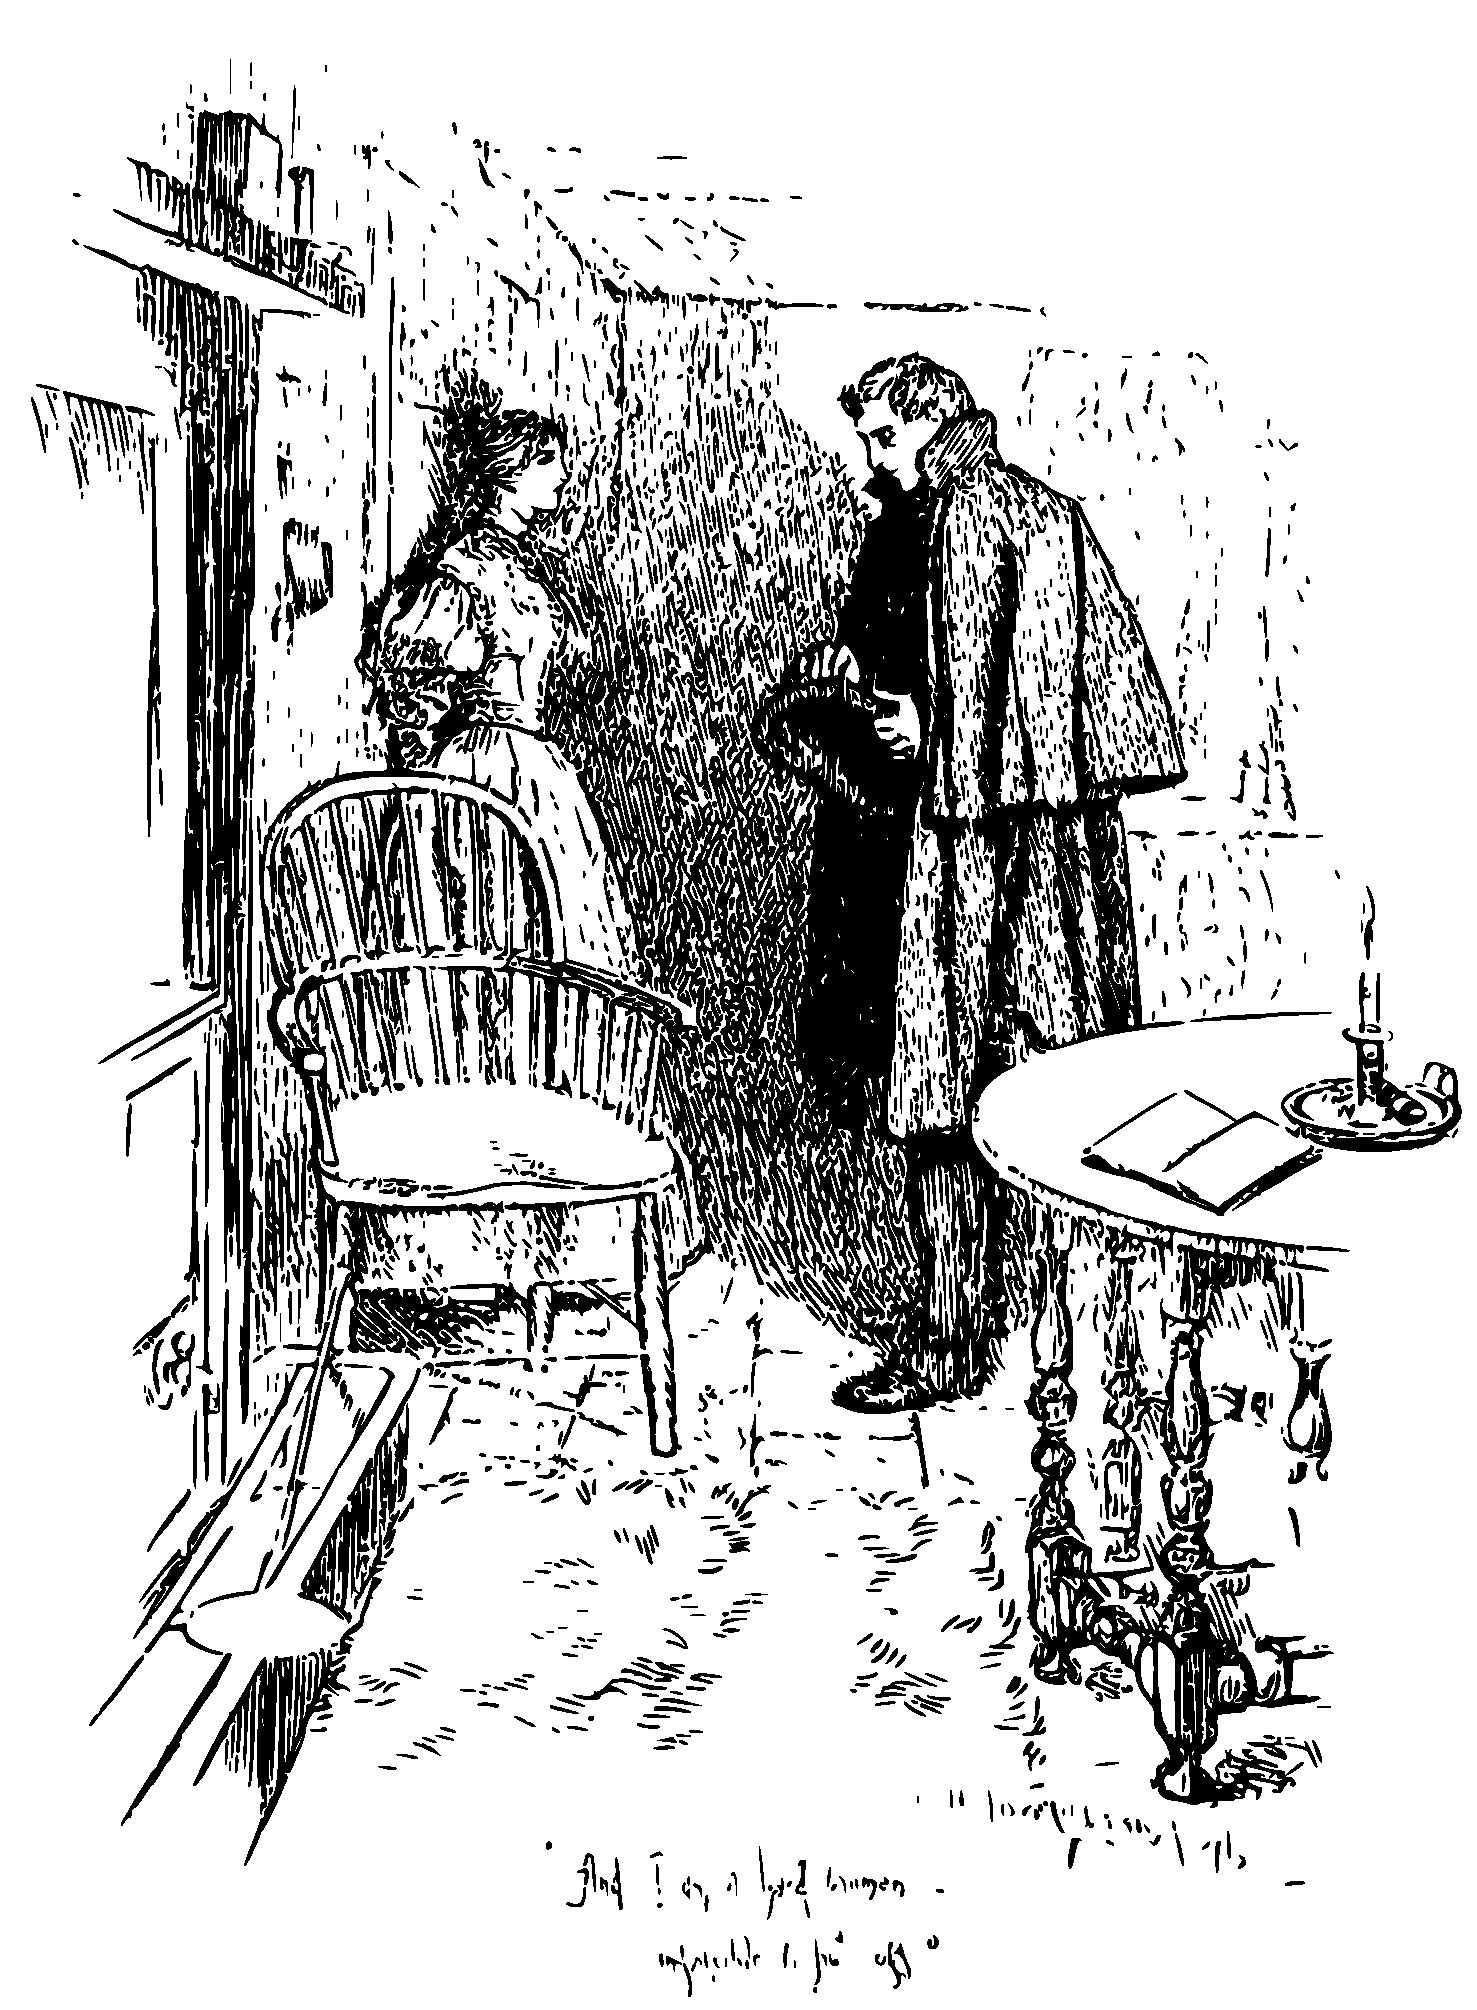
\includegraphics[width=\linewidth]{images/p369b.pdf}
	\end{sidecaption}
\end{figure}

\enquote{And then,} he pursued, \enquote{I am cold: no fervour infects
me.}

\enquote{Whereas I am hot, and fire dissolves ice. The blaze there has
thawed all the snow from your cloak; by the same token, it has streamed
on to my floor, and made it like a trampled street. As you hope ever to
be forgiven, \Mr{} Rivers, the high crime and misdemeanour of spoiling a
sanded kitchen, tell me what I wish to know.}

\enquote{Well, then,} he said, \enquote{I yield; if not to your
earnestness, to your perseverance: as stone is worn by continual
dropping. Besides, you must know some day,---as well now as later. 
Your name is Jane Eyre?}

\enquote{Of course: that was all settled before.}

\enquote{You are not, perhaps, aware that I am your namesake?---that I
was christened \St{} John Eyre Rivers?}

\enquote{No, indeed! I remember now seeing the letter E. comprised in
your initials written in books you have at different times lent me; but
I never asked for what name it stood. But what then? Surely---}

I stopped: I could not trust myself to entertain, much less to express,
the thought that rushed upon me---that embodied itself,---that, in a
second, stood out a strong, solid probability. Circumstances knit
themselves, fitted themselves, shot into order: the chain that had been
lying hitherto a formless lump of links was drawn out straight,---every
ring was perfect, the connection complete. I knew, by instinct, how the
matter stood, before \St{} John had said another word; but I cannot expect
the reader to have the same intuitive perception, so I must repeat his
explanation.

\enquote{My mother's name was Eyre; she had two brothers; one a
clergyman, who married Miss Jane Reed, of Gateshead; the other, John
Eyre, Esq., merchant, late of Funchal, Madeira. \Mr{} Briggs, being \Mr{}
Eyre's solicitor, wrote to us last August to inform us of our uncle's
death, and to say that he had left his property to his brother the
clergyman's orphan daughter, overlooking us, in consequence of a
quarrel, never forgiven, between him and my father. He wrote again a
few weeks since, to intimate that the heiress was lost, and asking if we
knew anything of her. A name casually written on a slip of paper has
enabled me to find her out. You know the rest.} Again he was going,
but I set my back against the door.

\enquote{Do let me speak,} I said; \enquote{let me have one moment to
draw breath and reflect.} I paused---he stood before me, hat in hand,
looking composed enough. I resumed---

\enquote{Your mother was my father's sister?}

\enquote{Yes.}

\enquote{My aunt, consequently?}

He bowed.

\enquote{My uncle John was your uncle John? You, Diana, and Mary are
his sister's children, as I am his brother's child?}

\enquote{Undeniably.}

\enquote{You three, then, are my cousins; half our blood on each side
flows from the same source?}

\enquote{We are cousins; yes.}

I surveyed him. It seemed I had found a brother: one I could be proud
of,---one I could love; and two sisters, whose qualities were such,
that, when I knew them but as mere strangers, they had inspired me with
genuine affection and admiration. The two girls, on whom, kneeling down
on the wet ground, and looking through the low, latticed window of Moor
House kitchen, I had gazed with so bitter a mixture of interest and
despair, were my near kinswomen; and the young and stately gentleman who
had found me almost dying at his threshold was my blood relation. 
Glorious discovery to a lonely wretch! This was wealth indeed!---wealth
to the heart!---a mine of pure, genial affections. This was a blessing,
bright, vivid, and exhilarating;---not like the ponderous gift of gold:
rich and welcome enough in its way, but sobering from its weight. I now
clapped my hands in sudden joy---my pulse bounded, my veins thrilled.

\enquote{Oh, I am glad!---I am glad!} I exclaimed.

\St{} John smiled. \enquote{Did I not say you neglected essential points
to pursue trifles?} he asked. \enquote{You were serious when I told you
you had got a fortune; and now, for a matter of no moment, you are
excited.}

\enquote{What can you mean? It may be of no moment to you; you have
sisters and don't care for a cousin; but I had nobody; and now three
relations,---or two, if you don't choose to be counted,---are born into
my world full-grown. I say again, I am glad!}

I walked fast through the room: I stopped, half suffocated with the
thoughts that rose faster than I could receive, comprehend, settle
them:---thoughts of what might, could, would, and should be, and that
ere long. I looked at the blank wall: it seemed a sky thick with
ascending stars,---every one lit me to a purpose or delight. Those who
had saved my life, whom, till this hour, I had loved barrenly, I could
now benefit. They were under a yoke,---I could free them: they were
scattered,---I could reunite them: the independence, the affluence which
was mine, might be theirs too. Were we not four? Twenty thousand
pounds shared equally would be five thousand each, justice---enough and
to spare: justice would be done,---mutual happiness secured. Now the
wealth did not weigh on me: now it was not a mere bequest of coin,---it
was a legacy of life, hope, enjoyment.

How I looked while these ideas were taking my spirit by storm, I cannot
tell; but I perceived soon that \Mr{} Rivers had placed a chair behind me,
and was gently attempting to make me sit down on it. He also advised me
to be composed; I scorned the insinuation of helplessness and
distraction, shook off his hand, and began to walk about again.

\enquote{Write to Diana and Mary to-morrow,} I said, \enquote{and tell
them to come home directly. Diana said they would both consider
themselves rich with a thousand pounds, so with five thousand they will
do very well.}

\enquote{Tell me where I can get you a glass of water,} said \St{} John;
\enquote{you must really make an effort to tranquillise your feelings.}

\enquote{Nonsense! and what sort of an effect will the bequest have on
you? Will it keep you in England, induce you to marry Miss Oliver, and
settle down like an ordinary mortal?}

\enquote{You wander: your head becomes confused. I have been too abrupt
in communicating the news; it has excited you beyond your strength.}

\enquote{\Mr{} Rivers! you quite put me out of patience: I am rational
enough; it is you who misunderstand, or rather who affect to
misunderstand.}

\enquote{Perhaps, if you explained yourself a little more fully, I
should comprehend better.}

\enquote{Explain! What is there to explain? You cannot fail to see
that twenty thousand pounds, the sum in question, divided equally
between the nephew and three nieces of our uncle, will give five
thousand to each? What I want is, that you should write to your sisters
and tell them of the fortune that has accrued to them.}

\enquote{To you, you mean.}

\enquote{I have intimated my view of the case: I am incapable of taking
any other. I am not brutally selfish, blindly unjust, or fiendishly
ungrateful. Besides, I am resolved I will have a home and connections. 
I like Moor House, and I will live at Moor House; I like Diana and Mary,
and I will attach myself for life to Diana and Mary. It would please
and benefit me to have five thousand pounds; it would torment and
oppress me to have twenty thousand; which, moreover, could never be mine
in justice, though it might in law. I abandon to you, then, what is
absolutely superfluous to me. Let there be no opposition, and no
discussion about it; let us agree amongst each other, and decide the
point at once.}

\enquote{This is acting on first impulses; you must take days to
consider such a matter, ere your word can be regarded as valid.}

\enquote{Oh! if all you doubt is my sincerity, I am easy: you see the
justice of the case?}

\enquote{I \emph{do} see a certain justice; but it is contrary to all custom. 
Besides, the entire fortune is your right: my uncle gained it by his own
efforts; he was free to leave it to whom he would: he left it to you. 
After all, justice permits you to keep it: you may, with a clear
conscience, consider it absolutely your own.}

\enquote{With me,} said I, \enquote{it is fully as much a matter of
feeling as of conscience: I must indulge my feelings; I so seldom have
had an opportunity of doing so. Were you to argue, object, and annoy me
for a year, I could not forego the delicious pleasure of which I have
caught a glimpse---that of repaying, in part, a mighty obligation, and
winning to myself lifelong friends.}

\enquote{You think so now,} rejoined \St{} John, \enquote{because you do
not know what it is to possess, nor consequently to enjoy wealth: you
cannot form a notion of the importance twenty thousand pounds would give
you; of the place it would enable you to take in society; of the
prospects it would open to you: you cannot---}

\enquote{And you,} I interrupted, \enquote{cannot at all imagine the
craving I have for fraternal and sisterly love. I never had a home, I
never had brothers or sisters; I must and will have them now: you are
not reluctant to admit me and own me, are you?}

\enquote{Jane, I will be your brother---my sisters will be your
sisters---without stipulating for this sacrifice of your just rights.}

\enquote{Brother? Yes; at the distance of a thousand leagues! 
Sisters? Yes; slaving amongst strangers! I, wealthy---gorged with gold
I never earned and do not merit! You, penniless! Famous equality and
fraternisation! Close union! Intimate attachment!}

\enquote{But, Jane, your aspirations after family ties and domestic
happiness may be realised otherwise than by the means you contemplate:
you may marry.}

\enquote{Nonsense, again! Marry! I don't want to marry, and never
shall marry.}

\enquote{That is saying too much: such hazardous affirmations are a
proof of the excitement under which you labour.}

\enquote{It is not saying too much: I know what I feel, and how averse
are my inclinations to the bare thought of marriage. No one would take
me for love; and I will not be regarded in the light of a mere money
speculation. And I do not want a stranger---unsympathising, alien,
different from me; I want my kindred: those with whom I have full
fellow-feeling. Say again you will be my brother: when you uttered the
words I was satisfied, happy; repeat them, if you can, repeat them
sincerely.}

\enquote{I think I can. I know I have always loved my own sisters; and
I know on what my affection for them is grounded,---respect for their
worth and admiration of their talents. You too have principle and mind:
your tastes and habits resemble Diana's and Mary's; your presence is
always agreeable to me; in your conversation I have already for some
time found a salutary solace. I feel I can easily and naturally make
room in my heart for you, as my third and youngest sister.}

\enquote{Thank you: that contents me for to-night. Now you had better
go; for if you stay longer, you will perhaps irritate me afresh by some
mistrustful scruple.}

\enquote{And the school, Miss Eyre? It must now be shut up, I suppose?}

\enquote{No. I will retain my post of mistress till you get a
substitute.}

He smiled approbation: we shook hands, and he took leave.

I need not narrate in detail the further struggles I had, and arguments
I used, to get matters regarding the legacy settled as I wished. My
task was a very hard one; but, as I was absolutely resolved---as my
cousins saw at length that my mind was really and immutably fixed on
making a just division of the property---as they must in their own
hearts have felt the equity of the intention; and must, besides, have
been innately conscious that in my place they would have done precisely
what I wished to do---they yielded at length so far as to consent to put
the affair to arbitration. The judges chosen were \Mr{} Oliver and an
able lawyer: both coincided in my opinion: I carried my point. The
instruments of transfer were drawn out: \St{} John, Diana, Mary, and I,
each became possessed of a competency.

\FChapter{Chapter Thirty-Four}{34}

\Lettrine{I}{t} \textsc{was near Christmas} by the time all was settled: the season of general
holiday approached. I now closed Morton school, taking care that the
parting should not be barren on my side. Good fortune opens the hand as
well as the heart wonderfully; and to give somewhat when we have largely
received, is but to afford a vent to the unusual ebullition of the
sensations. I had long felt with pleasure that many of my rustic
scholars liked me, and when we parted, that consciousness was confirmed:
they manifested their affection plainly and strongly. Deep was my
gratification to find I had really a place in their unsophisticated
hearts: I promised them that never a week should pass in future that I
did not visit them, and give them an hour's teaching in their school.

\Mr{} Rivers came up as, having seen the classes, now numbering sixty
girls, file out before me, and locked the door, I stood with the key in
my hand, exchanging a few words of special farewell with some half-dozen
of my best scholars: as decent, respectable, modest, and well-informed
young women as could be found in the ranks of the British peasantry.
And that is saying a great deal; for after all, the British peasantry
are the best taught, best mannered, most self-respecting of any in
Europe: since those days I have seen paysannes and Bäuerinnen; and the
best of them seemed to me ignorant, coarse, and besotted, compared with
my Morton girls.

\enquote{Do you consider you have got your reward for a season of
	exertion?} asked \Mr{} Rivers, when they were gone. \enquote{Does not the
	consciousness of having done some real good in your day and generation
	give pleasure?}

\enquote{Doubtless.}

\enquote{And you have only toiled a few months! Would not a life
	devoted to the task of regenerating your race be well spent?}

\enquote{Yes,} I said; \enquote{but I could not go on for ever so: I
	want to enjoy my own faculties as well as to cultivate those of other
	people. I must enjoy them now; don't recall either my mind or body to
	the school; I am out of it and disposed for full holiday.}

He looked grave. \enquote{What now? What sudden eagerness is this you
	evince? What are you going to do?}

\enquote{To be active: as active as I can. And first I must beg you to
	set Hannah at liberty, and get somebody else to wait on you.}

\enquote{Do you want her?}

\enquote{Yes, to go with me to Moor House. Diana and Mary will be at
	home in a week, and I want to have everything in order against their
	arrival.}

\enquote{I understand. I thought you were for flying off on some
	excursion. It is better so: Hannah shall go with you.}

\enquote{Tell her to be ready by to-morrow then; and here is the
	schoolroom key: I will give you the key of my cottage in the morning.}

He took it. \enquote{You give it up very gleefully,} said he;
\enquote{I don't quite understand your light-heartedness, because I
	cannot tell what employment you propose to yourself as a substitute for
	the one you are relinquishing. What aim, what purpose, what ambition in
	life have you now?}

\enquote{My first aim will be to \emph{clean down} (do you comprehend the full
	force of the expression?)---to \emph{clean down} Moor House from chamber
	to cellar; my next to rub it up with bees-wax, oil, and an indefinite
	number of cloths, till it glitters again; my third, to arrange every
	chair, table, bed, carpet, with mathematical precision; afterwards I
	shall go near to ruin you in coals and peat to keep up good fires in
	every room; and lastly, the two days preceding that on which your
	sisters are expected will be devoted by Hannah and me to such a beating
	of eggs, sorting of currants, grating of spices, compounding of
	Christmas cakes, chopping up of materials for mince-pies, and
	solemnising of other culinary rites, as words can convey but an
	inadequate notion of to the uninitiated like you. My purpose, in short,
	is to have all things in an absolutely perfect state of readiness for
	Diana and Mary before next Thursday; and my ambition is to give them a
	beau-ideal of a welcome when they come.}

\St{} John smiled slightly: still he was dissatisfied.

\enquote{It is all very well for the present,} said he; \enquote{but
	seriously, I trust that when the first flush of vivacity is over, you
	will look a little higher than domestic endearments and household joys.}

\enquote{The best things the world has!} I interrupted.

\enquote{No, Jane, no: this world is not the scene of fruition; do not
	attempt to make it so: nor of rest; do not turn slothful.}

\enquote{I mean, on the contrary, to be busy.}

\enquote{Jane, I excuse you for the present: two months' grace I allow you for
	the full enjoyment of your new position, and for pleasing yourself with
	this late-found charm of relationship; but \emph{then}, I hope you will
	begin to look beyond Moor House and Morton, and sisterly society, and
	the selfish calm and sensual comfort of civilised affluence. I hope
	your energies will then once more trouble you with their strength.}

I looked at him with surprise. \enquote{\St{} John,} I said, \enquote{I
	think you are almost wicked to talk so. I am disposed to be as content
	as a queen, and you try to stir me up to restlessness! To what end?}

\enquote{To the end of turning to profit the talents which God has
	committed to your keeping; and of which He will surely one day demand a
	strict account. Jane, I shall watch you closely and anxiously---I warn
	you of that. And try to restrain the disproportionate fervour with
	which you throw yourself into commonplace home pleasures. Don't cling
	so tenaciously to ties of the flesh; save your constancy and ardour for
	an adequate cause; forbear to waste them on trite transient objects. Do
	you hear, Jane?}

\enquote{Yes; just as if you were speaking Greek. I feel I have adequate cause
	to be happy, and I \emph{will} be happy. Goodbye!}

Happy at Moor House I was, and hard I worked; and so did Hannah: she was
charmed to see how jovial I could be amidst the bustle of a house turned
topsy-turvy---how I could brush, and dust, and clean, and cook. And
really, after a day or two of confusion worse confounded, it was
delightful by degrees to invoke order from the chaos ourselves had
made. I had previously taken a journey to S--- to purchase some new
furniture: my cousins having given me \emph{carte blanche} to effect
what alterations I pleased, and a sum having been set aside for that
purpose. The ordinary sitting-room and bedrooms I left much as they
were: for I knew Diana and Mary would derive more pleasure from seeing
again the old homely tables, and chairs, and beds, than from the
spectacle of the smartest innovations. Still some novelty was
necessary, to give to their return the piquancy with which I wished it
to be invested. Dark handsome new carpets and curtains, an arrangement
of some carefully selected antique ornaments in porcelain and bronze,
new coverings, and mirrors, and dressing-cases, for the toilet tables,
answered the end: they looked fresh without being glaring. A spare
parlour and bedroom I refurnished entirely, with old mahogany and
crimson upholstery: I laid canvas on the passage, and carpets on the
stairs. When all was finished, I thought Moor House as complete a model
of bright modest snugness within, as it was, at this season, a specimen
of wintry waste and desert dreariness without.

The eventful Thursday at length came. They were expected about dark,
and ere dusk fires were lit upstairs and below; the kitchen was in
perfect trim; Hannah and I were dressed, and all was in readiness.

\St{} John arrived first. I had entreated him to keep quite clear of the
house till everything was arranged: and, indeed, the bare idea of the
commotion, at once sordid and trivial, going on within its walls
sufficed to scare him to estrangement. He found me in the kitchen,
watching the progress of certain cakes for tea, then baking.
Approaching the hearth, he asked, \enquote{If I was at last satisfied
	with housemaid's work?} I answered by inviting him to accompany me on a
general inspection of the result of my labours. With some difficulty, I
got him to make the tour of the house. He just looked in at the doors I
opened; and when he had wandered upstairs and downstairs, he said I must
have gone through a great deal of fatigue and trouble to have effected
such considerable changes in so short a time: but not a syllable did he
utter indicating pleasure in the improved aspect of his abode.

This silence damped me. I thought perhaps the alterations had disturbed
some old associations he valued. I inquired whether this was the case:
no doubt in a somewhat crest-fallen tone.

\enquote{Not at all; he had, on the contrary, remarked that I had
	scrupulously respected every association: he feared, indeed, I must have
	bestowed more thought on the matter than it was worth. How many
	minutes, for instance, had I devoted to studying the arrangement of this
	very room?---By-the-bye, could I tell him where such a book was?}

I showed him the volume on the shelf: he took it down, and withdrawing
to his accustomed window recess, he began to read it.

Now, I did not like this, reader. \St{} John was a good man; but I began
to feel he had spoken truth of himself when he said he was hard and
cold. The humanities and amenities of life had no attraction for
him---its peaceful enjoyments no charm. Literally, he lived only to
aspire---after what was good and great, certainly; but still he would
never rest, nor approve of others resting round him. As I looked at his
lofty forehead, still and pale as a white stone---at his fine lineaments
fixed in study---I comprehended all at once that he would hardly make a
good husband: that it would be a trying thing to be his wife. I
understood, as by inspiration, the nature of his love for Miss Oliver; I
agreed with him that it was but a love of the senses. I comprehended
how he should despise himself for the feverish influence it exercised
over him; how he should wish to stifle and destroy it; how he should
mistrust its ever conducting permanently to his happiness or hers. I
saw he was of the material from which nature hews her heroes---Christian
and Pagan---her lawgivers, her statesmen, her conquerors: a steadfast
bulwark for great interests to rest upon; but, at the fireside, too
often a cold cumbrous column, gloomy and out of place.

\enquote{This parlour is not his sphere,} I reflected: \enquote{the
	Himalayan ridge or Caffre bush, even the plague-cursed Guinea Coast
	swamp would suit him better. Well may he eschew the calm of domestic
	life; it is not his element: there his faculties stagnate---they cannot
	develop or appear to advantage. It is in scenes of strife and
	danger---where courage is proved, and energy exercised, and fortitude
	tasked---that he will speak and move, the leader and superior. A merry
	child would have the advantage of him on this hearth. He is right to
	choose a missionary's career---I see it now.}

\enquote{They are coming! they are coming!} cried Hannah, throwing open
the parlour door. At the same moment old Carlo barked joyfully. Out I
ran. It was now dark; but a rumbling of wheels was audible. Hannah
soon had a lantern lit. The vehicle had stopped at the wicket; the
driver opened the door: first one well-known form, then another, stepped
out. In a minute I had my face under their bonnets, in contact first
with Mary's soft cheek, then with Diana's flowing curls. They
laughed---kissed me---then Hannah: patted Carlo, who was half wild with
delight; asked eagerly if all was well; and being assured in the
affirmative, hastened into the house.

They were stiff with their long and jolting drive from Whitcross, and
chilled with the frosty night air; but their pleasant countenances
expanded to the cheerful firelight. While the driver and Hannah brought
in the boxes, they demanded \St{} John. At this moment he advanced from
the parlour. They both threw their arms round his neck at once. He
gave each one quiet kiss, said in a low tone a few words of welcome,
stood a while to be talked to, and then, intimating that he supposed
they would soon rejoin him in the parlour, withdrew there as to a place
of refuge.

I had lit their candles to go upstairs, but Diana had first to give
hospitable orders respecting the driver; this done, both followed me.
They were delighted with the renovation and decorations of their rooms;
with the new drapery, and fresh carpets, and rich tinted china vases:
they expressed their gratification ungrudgingly. I had the pleasure of
feeling that my arrangements met their wishes exactly, and that what I
had done added a vivid charm to their joyous return home.

Sweet was that evening. My cousins, full of exhilaration, were so
eloquent in narrative and comment, that their fluency covered \St{} John's
taciturnity: he was sincerely glad to see his sisters; but in their glow
of fervour and flow of joy he could not sympathise. The event of the
day---that is, the return of Diana and Mary---pleased him; but the
accompaniments of that event, the glad tumult, the garrulous glee of
reception irked him: I saw he wished the calmer morrow was come. In the
very meridian of the night's enjoyment, about an hour after tea, a rap
was heard at the door. Hannah entered with the intimation that
\enquote{a poor lad was come, at that unlikely time, to fetch \Mr{} Rivers
	to see his mother, who was drawing away.}

\enquote{Where does she live, Hannah?}

\enquote{Clear up at Whitcross Brow, almost four miles off, and moor and
	moss all the way.}

\enquote{Tell him I will go.}

\enquote{I'm sure, sir, you had better not. It's the worst road to
	travel after dark that can be: there's no track at all over the bog.
	And then it is such a bitter night---the keenest wind you ever felt.
	You had better send word, sir, that you will be there in the morning.}

But he was already in the passage, putting on his cloak; and without one
objection, one murmur, he departed. It was then nine o'clock: he did
not return till midnight. Starved and tired enough he was: but he
looked happier than when he set out. He had performed an act of duty;
made an exertion; felt his own strength to do and deny, and was on
better terms with himself.

I am afraid the whole of the ensuing week tried his patience. It was
Christmas week: we took to no settled employment, but spent it in a sort
of merry domestic dissipation. The air of the moors, the freedom of
home, the dawn of prosperity, acted on Diana and Mary's spirits like
some life-giving elixir: they were gay from morning till noon, and from
noon till night. They could always talk; and their discourse, witty,
pithy, original, had such charms for me, that I preferred listening to,
and sharing in it, to doing anything else. \St{} John did not rebuke our
vivacity; but he escaped from it: he was seldom in the house; his parish
was large, the population scattered, and he found daily business in
visiting the sick and poor in its different districts.

One morning at breakfast, Diana, after looking a little pensive for some
minutes, asked him, \enquote{If his plans were yet unchanged.}

\enquote{Unchanged and unchangeable,} was the reply. And he proceeded
to inform us that his departure from England was now definitively fixed
for the ensuing year.

\enquote{And Rosamond Oliver?} suggested Mary, the words seeming to
escape her lips involuntarily: for no sooner had she uttered them, than
she made a gesture as if wishing to recall them. \St{} John had a book in
his hand---it was his unsocial custom to read at meals---he closed it,
and looked up.

\enquote{Rosamond Oliver,} said he, \enquote{is about to be married to
	\Mr{} Granby, one of the best connected and most estimable residents in
	S-, grandson and heir to Sir Frederic Granby: I had the intelligence
	from her father yesterday.}

His sisters looked at each other and at me; we all three looked at him:
he was serene as glass.

\enquote{The match must have been got up hastily,} said Diana:
\enquote{they cannot have known each other long.}

\enquote{But two months: they met in October at the county ball at S-.
	But where there are no obstacles to a union, as in the present case,
	where the connection is in every point desirable, delays are
	unnecessary: they will be married as soon as S--- Place, which Sir
	Frederic gives up to them, can he refitted for their reception.}

The first time I found \St{} John alone after this communication, I felt
tempted to inquire if the event distressed him: but he seemed so little
to need sympathy, that, so far from venturing to offer him more, I
experienced some shame at the recollection of what I had already
hazarded. Besides, I was out of practice in talking to him: his reserve
was again frozen over, and my frankness was congealed beneath it. He
had not kept his promise of treating me like his sisters; he continually
made little chilling differences between us, which did not at all tend
to the development of cordiality: in short, now that I was acknowledged
his kinswoman, and lived under the same roof with him, I felt the
distance between us to be far greater than when he had known me only as
the village schoolmistress. When I remembered how far I had once been
admitted to his confidence, I could hardly comprehend his present
frigidity.

Such being the case, I felt not a little surprised when he raised his
head suddenly from the desk over which he was stooping, and said---

\enquote{You see, Jane, the battle is fought and the victory won.}

Startled at being thus addressed, I did not immediately reply: after a
moment's hesitation I answered---

\enquote{But are you sure you are not in the position of those
	conquerors whose triumphs have cost them too dear? Would not such
	another ruin you?}

\enquote{I think not; and if I were, it does not much signify; I shall
	never be called upon to contend for such another. The event of the
	conflict is decisive: my way is now clear; I thank God for it!} So
saying, he returned to his papers and his silence.

As our mutual happiness (\emph{\ie}, Diana's, Mary's, and mine) settled
into a quieter character, and we resumed our usual habits and regular
studies, \St{} John stayed more at home: he sat with us in the same room,
sometimes for hours together. While Mary drew, Diana pursued a course
of encyclopædic reading she had (to my awe and amazement) undertaken,
and I fagged away at German, he pondered a mystic lore of his own: that
of some Eastern tongue, the acquisition of which he thought necessary to
his plans.

Thus engaged, he appeared, sitting in his own recess, quiet and absorbed
enough; but that blue eye of his had a habit of leaving the
outlandish-looking grammar, and wandering over, and sometimes fixing
upon us, his fellow-students, with a curious intensity of observation:
if caught, it would be instantly withdrawn; yet ever and anon, it
returned searchingly to our table. I wondered what it meant: I
wondered, too, at the punctual satisfaction he never failed to exhibit
on an occasion that seemed to me of small moment, namely, my weekly
visit to Morton school; and still more was I puzzled when, if the day
was unfavourable, if there was snow, or rain, or high wind, and his
sisters urged me not to go, he would invariably make light of their
solicitude, and encourage me to accomplish the task without regard to
the elements.

\enquote{Jane is not such a weakling as you would make her,} he would
say: \enquote{she can bear a mountain blast, or a shower, or a few
	flakes of snow, as well as any of us. Her constitution is both sound
	and elastic;---better calculated to endure variations of climate than
	many more robust.}

And when I returned, sometimes a good deal tired, and not a little
weather-beaten, I never dared complain, because I saw that to murmur
would be to vex him: on all occasions fortitude pleased him; the reverse
was a special annoyance.

One afternoon, however, I got leave to stay at home, because I really
had a cold. His sisters were gone to Morton in my stead: I sat reading
Schiller; he, deciphering his crabbed Oriental scrolls. As I exchanged
a translation for an exercise, I happened to look his way: there I found
myself under the influence of the ever-watchful blue eye. How long it
had been searching me through and through, and over and over, I cannot
tell: so keen was it, and yet so cold, I felt for the moment
superstitious---as if I were sitting in the room with something uncanny.

\enquote{Jane, what are you doing?}

\enquote{Learning German.}

\enquote{I want you to give up German and learn Hindostanee.}

\enquote{You are not in earnest?}

\enquote{In such earnest that I must have it so: and I will tell you
	why.}

He then went on to explain that Hindostanee was the language he was
himself at present studying; that, as he advanced, he was apt to forget
the commencement; that it would assist him greatly to have a pupil with
whom he might again and again go over the elements, and so fix them
thoroughly in his mind; that his choice had hovered for some time
between me and his sisters; but that he had fixed on me because he saw I
could sit at a task the longest of the three. Would I do him this
favour? I should not, perhaps, have to make the sacrifice long, as it
wanted now barely three months to his departure.

\St{} John was not a man to be lightly refused: you felt that every
impression made on him, either for pain or pleasure, was deep-graved and
permanent. I consented. When Diana and Mary returned, the former found
her scholar transferred from her to her brother: she laughed, and both
she and Mary agreed that \St{} John should never have persuaded them to
such a step. He answered quietly---

\enquote{I know it.}

I found him a very patient, very forbearing, and yet an exacting master:
he expected me to do a great deal; and when I fulfilled his
expectations, he, in his own way, fully testified his approbation. By
degrees, he acquired a certain influence over me that took away my
liberty of mind: his praise and notice were more restraining than his
indifference. I could no longer talk or laugh freely when he was by,
because a tiresomely importunate instinct reminded me that vivacity (at
least in me) was distasteful to him. I was so fully aware that only
serious moods and occupations were acceptable, that in his presence
every effort to sustain or follow any other became vain: I fell under a
freezing spell. When he said \enquote{go,} I went; \enquote{come,} I
came; \enquote{do this,} I did it. But I did not love my servitude: I
wished, many a time, he had continued to neglect me.

One evening when, at bedtime, his sisters and I stood round him, bidding
him good-night, he kissed each of them, as was his custom; and, as was
equally his custom, he gave me his hand. Diana, who chanced to be in a
frolicsome humour (\emph{she} was not painfully controlled by his will;
for hers, in another way, was as strong), exclaimed---

\enquote{\St{} John! you used to call Jane your third sister, but you
	don't treat her as such: you should kiss her too.}

She pushed me towards him. I thought Diana very provoking, and felt
uncomfortably confused; and while I was thus thinking and feeling, St.
John bent his head; his Greek face was brought to a level with mine, his
eyes questioned my eyes piercingly---he kissed me. There are no such
things as marble kisses or ice kisses, or I should say my ecclesiastical
cousin's salute belonged to one of these classes; but there may be
experiment kisses, and his was an experiment kiss. When given, he
viewed me to learn the result; it was not striking: I am sure I did not
blush; perhaps I might have turned a little pale, for I felt as if this
kiss were a seal affixed to my fetters. He never omitted the ceremony
afterwards, and the gravity and quiescence with which I underwent it,
seemed to invest it for him with a certain charm.

As for me, I daily wished more to please him; but to do so, I felt daily
more and more that I must disown half my nature, stifle half my
faculties, wrest my tastes from their original bent, force myself to the
adoption of pursuits for which I had no natural vocation. He wanted to
train me to an elevation I could never reach; it racked me hourly to
aspire to the standard he uplifted. The thing was as impossible as to
mould my irregular features to his correct and classic pattern, to give
to my changeable green eyes the sea-blue tint and solemn lustre of his
own.

Not his ascendancy alone, however, held me in thrall at present. Of
late it had been easy enough for me to look sad: a cankering evil sat at
my heart and drained my happiness at its source---the evil of suspense.

Perhaps you think I had forgotten \Mr{} Rochester, reader, amidst these
changes of place and fortune. Not for a moment. His idea was still
with me, because it was not a vapour sunshine could disperse, nor a
sand-traced effigy storms could wash away; it was a name graven on a
tablet, fated to last as long as the marble it inscribed. The craving
to know what had become of him followed me everywhere; when I was at
Morton, I re-entered my cottage every evening to think of that; and now
at Moor House, I sought my bedroom each night to brood over it.

In the course of my necessary correspondence with \Mr{} Briggs about the
will, I had inquired if he knew anything of \Mr{} Rochester's present
residence and state of health; but, as \St{} John had conjectured, he was
quite ignorant of all concerning him. I then wrote to \Mrs{} Fairfax,
entreating information on the subject. I had calculated with certainty
on this step answering my end: I felt sure it would elicit an early
answer. I was astonished when a fortnight passed without reply; but
when two months wore away, and day after day the post arrived and
brought nothing for me, I fell a prey to the keenest anxiety.

I wrote again: there was a chance of my first letter having missed.
Renewed hope followed renewed effort: it shone like the former for some
weeks, then, like it, it faded, flickered: not a line, not a word
reached me. When half a year wasted in vain expectancy, my hope died
out, and then I felt dark indeed.

A fine spring shone round me, which I could not enjoy. Summer
approached; Diana tried to cheer me: she said I looked ill, and wished
to accompany me to the sea-side. This \St{} John opposed; he said I did
not want dissipation, I wanted employment; my present life was too
purposeless, I required an aim; and, I suppose, by way of supplying
deficiencies, he prolonged still further my lessons in Hindostanee, and
grew more urgent in requiring their accomplishment: and I, like a fool,
never thought of resisting him---I could not resist him.

One day I had come to my studies in lower spirits than usual; the ebb
was occasioned by a poignantly felt disappointment. Hannah had told me
in the morning there was a letter for me, and when I went down to take
it, almost certain that the long-looked for tidings were vouchsafed me
at last, I found only an unimportant note from \Mr{} Briggs on business.
The bitter check had wrung from me some tears; and now, as I sat poring
over the crabbed characters and flourishing tropes of an Indian scribe,
my eyes filled again.

\St{} John called me to his side to read; in attempting to do this my
voice failed me: words were lost in sobs. He and I were the only
occupants of the parlour: Diana was practising her music in the
drawing-room, Mary was gardening---it was a very fine May day, clear,
sunny, and breezy. My companion expressed no surprise at this emotion,
nor did he question me as to its cause; he only said---

\enquote{We will wait a few minutes, Jane, till you are more composed.}
And while I smothered the paroxysm with all haste, he sat calm and
patient, leaning on his desk, and looking like a physician watching with
the eye of science an expected and fully understood crisis in a
patient's malady. Having stifled my sobs, wiped my eyes, and muttered
something about not being very well that morning, I resumed my task, and
succeeded in completing it. \St{} John put away my books and his, locked
his desk, and said---

\enquote{Now, Jane, you shall take a walk; and with me.}

\enquote{I will call Diana and Mary.}

\enquote{No; I want only one companion this morning, and that must be
	you. Put on your things; go out by the kitchen-door: take the road
	towards the head of Marsh Glen: I will join you in a moment.}

I know no medium: I never in my life have known any medium in my
dealings with positive, hard characters, antagonistic to my own, between
absolute submission and determined revolt. I have always faithfully
observed the one, up to the very moment of bursting, sometimes with
volcanic vehemence, into the other; and as neither present circumstances
warranted, nor my present mood inclined me to mutiny, I observed careful
obedience to \St{} John's directions; and in ten minutes I was treading
the wild track of the glen, side by side with him.

The breeze was from the west: it came over the hills, sweet with scents
of heath and rush; the sky was of stainless blue; the stream descending
the ravine, swelled with past spring rains, poured along plentiful and
clear, catching golden gleams from the sun, and sapphire tints from the
firmament. As we advanced and left the track, we trod a soft turf,
mossy fine and emerald green, minutely enamelled with a tiny white
flower, and spangled with a star-like yellow blossom: the hills,
meantime, shut us quite in; for the glen, towards its head, wound to
their very core.

\enquote{Let us rest here,} said \St{} John, as we reached the first
stragglers of a battalion of rocks, guarding a sort of pass, beyond
which the beck rushed down a waterfall; and where, still a little
farther, the mountain shook off turf and flower, had only heath for
raiment and crag for gem---where it exaggerated the wild to the savage,
and exchanged the fresh for the frowning---where it guarded the forlorn
hope of solitude, and a last refuge for silence.

I took a seat: \St{} John stood near me. He looked up the pass and down
the hollow; his glance wandered away with the stream, and returned to
traverse the unclouded heaven which coloured it: he removed his hat, let
the breeze stir his hair and kiss his brow. He seemed in communion with
the genius of the haunt: with his eye he bade farewell to something.

\enquote{And I shall see it again,} he said aloud, \enquote{in dreams
	when I sleep by the Ganges: and again in a more remote hour---when
	another slumber overcomes me---on the shore of a darker stream!}

Strange words of a strange love! An austere patriot's passion for his
fatherland! He sat down; for half-an-hour we never spoke; neither he to
me nor I to him: that interval past, he recommenced---

\enquote{Jane, I go in six weeks; I have taken my berth in an East
	Indiaman which sails on the 20th of June.}

\enquote{God will protect you; for you have undertaken His work,} I
answered.

\enquote{Yes,} said he, \enquote{there is my glory and joy. I am the
	servant of an infallible Master. I am not going out under human
	guidance, subject to the defective laws and erring control of my feeble
	fellow-worms: my king, my lawgiver, my captain, is the All-perfect. It
	seems strange to me that all round me do not burn to enlist under the
	same banner,---to join in the same enterprise.}

\enquote{All have not your powers, and it would be folly for the feeble
	to wish to march with the strong.}

\enquote{I do not speak to the feeble, or think of them: I address only
	such as are worthy of the work, and competent to accomplish it.}

\enquote{Those are few in number, and difficult to discover.}

\enquote{You say truly; but when found, it is right to stir them up---to
	urge and exhort them to the effort---to show them what their gifts are,
	and why they were given---to speak Heaven's message in their ear,---to
	offer them, direct from God, a place in the ranks of His chosen.}

\enquote{If they are really qualified for the task, will not their own
	hearts be the first to inform them of it?}

I felt as if an awful charm was framing round and gathering over me: I
trembled to hear some fatal word spoken which would at once declare and
rivet the spell.

\enquote{And what does \emph{your} heart say?} demanded \St{} John.

\enquote{My heart is mute,---my heart is mute,} I answered, struck and
thrilled.

\enquote{Then I must speak for it,} continued the deep, relentless
voice. \enquote{Jane, come with me to India: come as my helpmeet and
	fellow-labourer.}

The glen and sky spun round: the hills heaved! It was as if I had heard
a summons from Heaven---as if a visionary messenger, like him of
Macedonia, had enounced, \enquote{Come over and help us!} But I was no
apostle,---I could not behold the herald,---I could not receive his
call.

\enquote{Oh, \St{} John!} I cried, \enquote{have some mercy!}

I appealed to one who, in the discharge of what he believed his duty,
knew neither mercy nor remorse. He continued---

\enquote{God and nature intended you for a missionary's wife. It is not
	personal, but mental endowments they have given you: you are formed for
	labour, not for love. A missionary's wife you must---shall be. You
	shall be mine: I claim you---not for my pleasure, but for my Sovereign's
	service.}

\enquote{I am not fit for it: I have no vocation,} I said.

He had calculated on these first objections: he was not irritated by
them. Indeed, as he leaned back against the crag behind him, folded his
arms on his chest, and fixed his countenance, I saw he was prepared for
a long and trying opposition, and had taken in a stock of patience to
last him to its close---resolved, however, that that close should be
conquest for him.

\enquote{Humility, Jane,} said he, \enquote{is the groundwork of
	Christian virtues: you say right that you are not fit for the work. Who
	is fit for it? Or who, that ever was truly called, believed himself
	worthy of the summons? I, for instance, am but dust and ashes. With
	\St{} Paul, I acknowledge myself the chiefest of sinners; but I do not
	suffer this sense of my personal vileness to daunt me. I know my
	Leader: that He is just as well as mighty; and while He has chosen a
	feeble instrument to perform a great task, He will, from the boundless
	stores of His providence, supply the inadequacy of the means to the
	end. Think like me, Jane---trust like me. It is the Rock of Ages I ask
	you to lean on: do not doubt but it will bear the weight of your human
	weakness.}

\enquote{I do not understand a missionary life: I have never studied
	missionary labours.}

\enquote{There I, humble as I am, can give you the aid you want: I can
	set you your task from hour to hour; stand by you always; help you from
	moment to moment. This I could do in the beginning: soon (for I know
	your powers) you would be as strong and apt as myself, and would not
	require my help.}

\enquote{But my powers---where are they for this undertaking? I do not
	feel them. Nothing speaks or stirs in me while you talk. I am sensible
	of no light kindling---no life quickening---no voice counselling or
	cheering. Oh, I wish I could make you see how much my mind is at this
	moment like a rayless dungeon, with one shrinking fear fettered in its
	depths---the fear of being persuaded by you to attempt what I cannot
	accomplish!}

\enquote{I have an answer for you---hear it. I have watched you ever
	since we first met: I have made you my study for ten months. I have
	proved you in that time by sundry tests: and what have I seen and
	elicited? In the village school I found you could perform well,
	punctually, uprightly, labour uncongenial to your habits and
	inclinations; I saw you could perform it with capacity and tact: you
	could win while you controlled. In the calm with which you learnt you
	had become suddenly rich, I read a mind clear of the vice of
	Demas:---lucre had no undue power over you. In the resolute readiness
	with which you cut your wealth into four shares, keeping but one to
	yourself, and relinquishing the three others to the claim of abstract
	justice, I recognised a soul that revelled in the flame and excitement
	of sacrifice. In the tractability with which, at my wish, you forsook a
	study in which you were interested, and adopted another because it
	interested me; in the untiring assiduity with which you have since
	persevered in it---in the unflagging energy and unshaken temper with
	which you have met its difficulties---I acknowledge the complement of
	the qualities I seek. Jane, you are docile, diligent, disinterested,
	faithful, constant, and courageous; very gentle, and very heroic: cease
	to mistrust yourself---I can trust you unreservedly. As a conductress
	of Indian schools, and a helper amongst Indian women, your assistance
	will be to me invaluable.}

My iron shroud contracted round me; persuasion advanced with slow sure
step. Shut my eyes as I would, these last words of his succeeded in
making the way, which had seemed blocked up, comparatively clear. My
work, which had appeared so vague, so hopelessly diffuse, condensed
itself as he proceeded, and assumed a definite form under his shaping
hand. He waited for an answer. I demanded a quarter of an hour to
think, before I again hazarded a reply.

\enquote{Very willingly,} he rejoined; and rising, he strode a little
distance up the pass, threw himself down on a swell of heath, and there
lay still.

\begin{figure}
	\begin{sidecaption}{\enquote{Threw himself down on\linebreak a swell of heath,\linebreak and there lay still.}}[p389b]
		\centering
		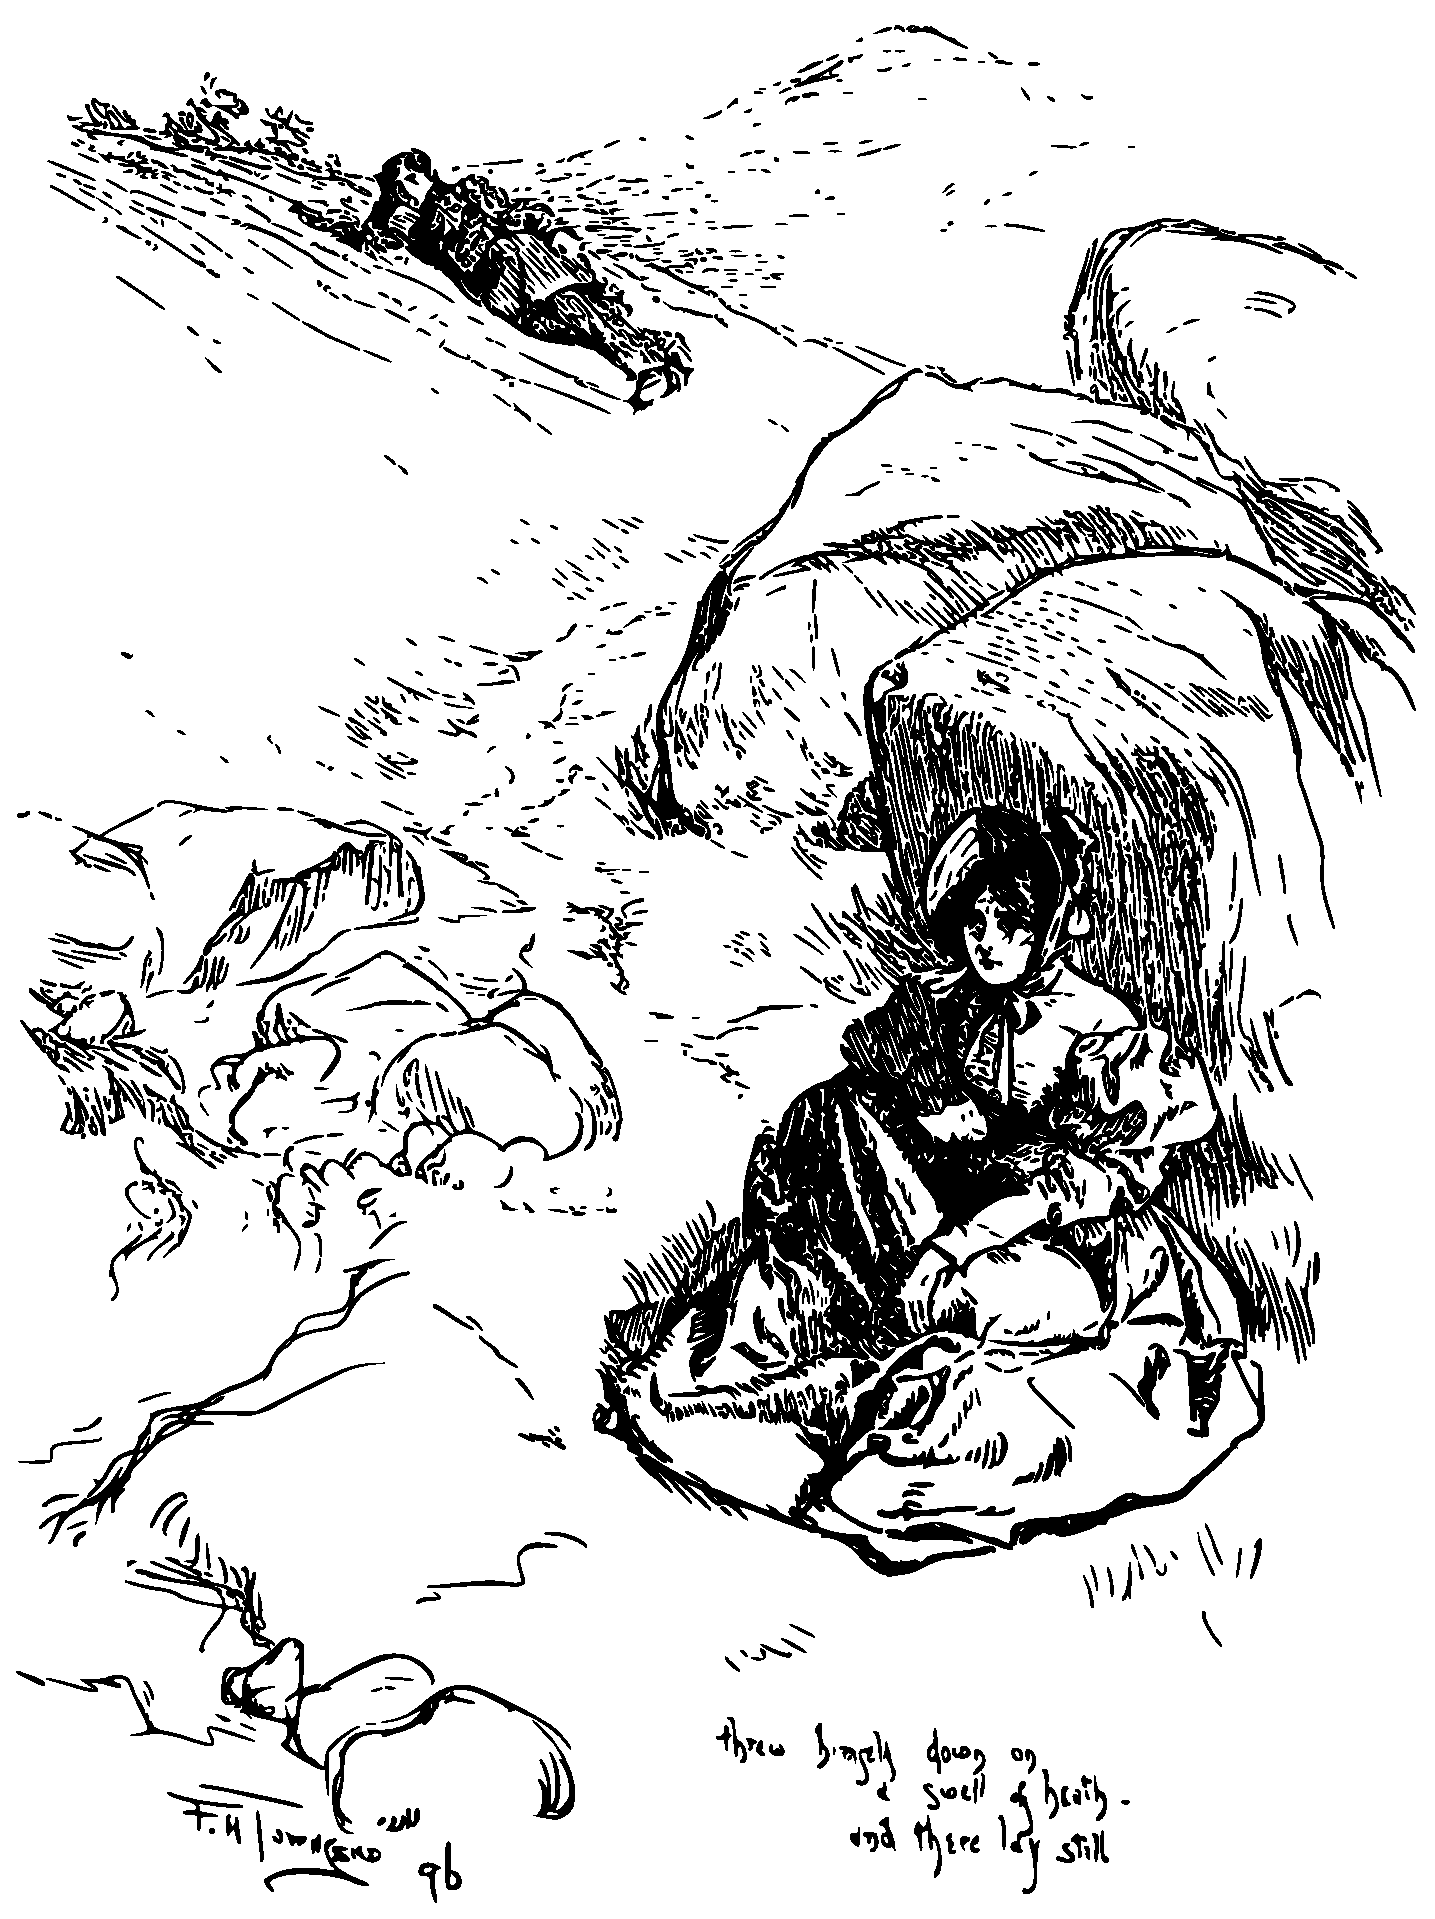
\includegraphics[width=\linewidth]{images/p389b.pdf}
	\end{sidecaption}
\end{figure}

\enquote{I \emph{can} do what he wants me to do: I am forced to see and
	acknowledge that,} I meditated,---\enquote{that is, if life be spared me. But
	I feel mine is not the existence to be long protracted under an Indian
	sun. What then? He does not care for that: when my time came to die,
	he would resign me, in all serenity and sanctity, to the God who gave
	me. The case is very plain before me. In leaving England, I should
	leave a loved but empty land---\Mr{} Rochester is not there; and if he
	were, what is, what can that ever be to me? My business is to live
	without him now: nothing so absurd, so weak as to drag on from day to
	day, as if I were waiting some impossible change in circumstances, which
	might reunite me to him. Of course (as \St{} John once said) I must seek
	another interest in life to replace the one lost: is not the occupation
	he now offers me truly the most glorious man can adopt or God assign?
	Is it not, by its noble cares and sublime results, the one best
	calculated to fill the void left by uptorn affections and demolished
	hopes? I believe I must say, Yes---and yet I shudder. Alas! If I join
	\St{} John, I abandon half myself: if I go to India, I go to premature
	death. And how will the interval between leaving England for India, and
	India for the grave, be filled? Oh, I know well! That, too, is very
	clear to my vision. By straining to satisfy \St{} John till my sinews
	ache, I \emph{shall} satisfy him---to the finest central point and
	farthest outward circle of his expectations. If I \emph{do} go with
	him---if I \emph{do} make the sacrifice he urges, I will make it
	absolutely: I will throw all on the altar---heart, vitals, the entire
	victim. He will never love me; but he shall approve me; I will show him
	energies he has not yet seen, resources he has never suspected. Yes, I
	can work as hard as he can, and with as little grudging.

	%rem enq
	Consent, then, to his demand is possible: but for one
	item---one dreadful item. It is---that he asks me to be his wife, and
	has no more of a husband's heart for me than that frowning giant of a
	rock, down which the stream is foaming in yonder gorge. He prizes me as
	a soldier would a good weapon; and that is all. Unmarried to him, this
	would never grieve me; but can I let him complete his
	calculations---coolly put into practice his plans---go through the
	wedding ceremony? Can I receive from him the bridal ring, endure all
	the forms of love (which I doubt not he would scrupulously observe) and
	know that the spirit was quite absent? Can I bear the consciousness
	that every endearment he bestows is a sacrifice made on principle? No:
	such a martyrdom would be monstrous. I will never undergo it. As his
	sister, I might accompany him---not as his wife: I will tell him so.}

I looked towards the knoll: there he lay, still as a prostrate column;
his face turned to me: his eye beaming watchful and keen. He started to
his feet and approached me.

\enquote{I am ready to go to India, if I may go free.}

\enquote{Your answer requires a commentary,} he said; \enquote{it is not
	clear.}

\enquote{You have hitherto been my adopted brother---I, your adopted
	sister: let us continue as such: you and I had better not marry.}

He shook his head. \enquote{Adopted fraternity will not do in this
	case. If you were my real sister it would be different: I should take
	you, and seek no wife. But as it is, either our union must be
	consecrated and sealed by marriage, or it cannot exist: practical
	obstacles oppose themselves to any other plan. Do you not see it,
	Jane? Consider a moment---your strong sense will guide you.}

I did consider; and still my sense, such as it was, directed me only to
the fact that we did not love each other as man and wife should: and
therefore it inferred we ought not to marry. I said so. \enquote{St.
	John,} I returned, \enquote{I regard you as a brother---you, me as a
	sister: so let us continue.}

\enquote{We cannot---we cannot,} he answered, with short, sharp
determination: \enquote{it would not do. You have said you will go with
	me to India: remember---you have said that.}

\enquote{Conditionally.}

\enquote{Well---well. To the main point---the departure with me from
	England, the co-operation with me in my future labours---you do not
	object. You have already as good as put your hand to the plough: you
	are too consistent to withdraw it. You have but one end to keep in
	view---how the work you have undertaken can best be done. Simplify your
	complicated interests, feelings, thoughts, wishes, aims; merge all
	considerations in one purpose: that of fulfilling with effect---with
	power---the mission of your great Master. To do so, you must have a
	coadjutor: not a brother---that is a loose tie---but a husband. I, too,
	do not want a sister: a sister might any day be taken from me. I want a
	wife: the sole helpmeet I can influence efficiently in life, and retain
	absolutely till death.}

I shuddered as he spoke: I felt his influence in my marrow---his hold on
my limbs.

\enquote{Seek one elsewhere than in me, \St{} John: seek one fitted to
	you.}

\enquote{One fitted to my purpose, you mean---fitted to my vocation.
	Again I tell you it is not the insignificant private individual---the
	mere man, with the man's selfish senses---I wish to mate: it is the
	missionary.}

\enquote{And I will give the missionary my energies---it is all he
	wants---but not myself: that would be only adding the husk and shell to
	the kernel. For them he has no use: I retain them.}

\enquote{You cannot---you ought not. Do you think God will be satisfied
	with half an oblation? Will He accept a mutilated sacrifice? It is the
	cause of God I advocate: it is under His standard I enlist you. I
	cannot accept on His behalf a divided allegiance: it must be entire.}

\enquote{Oh! I will give my heart to God,} I said. \enquote{\emph{You} do not
	want it.}

I will not swear, reader, that there was not something of repressed
sarcasm both in the tone in which I uttered this sentence, and in the
feeling that accompanied it. I had silently feared \St{} John till now,
because I had not understood him. He had held me in awe, because he had
held me in doubt. How much of him was saint, how much mortal, I could
not heretofore tell: but revelations were being made in this conference:
the analysis of his nature was proceeding before my eyes. I saw his
fallibilities: I comprehended them. I understood that, sitting there
where I did, on the bank of heath, and with that handsome form before
me, I sat at the feet of a man, caring as I\@. The veil fell from his
hardness and despotism. Having felt in him the presence of these
qualities, I felt his imperfection and took courage. I was with an
equal---one with whom I might argue---one whom, if I saw good, I might
resist.

He was silent after I had uttered the last sentence, and I presently
risked an upward glance at his countenance.

His eye, bent on me, expressed at once stern surprise and keen inquiry.
\enquote{Is she sarcastic, and sarcastic to \emph{me}!} it seemed to say.
\enquote{What does this signify?}

\enquote{Do not let us forget that this is a solemn matter,} he said ere
long; \enquote{one of which we may neither think nor talk lightly
	without sin. I trust, Jane, you are in earnest when you say you will
	serve your heart to God: it is all I want. Once wrench your heart from
	man, and fix it on your Maker, the advancement of that Maker's spiritual
	kingdom on earth will be your chief delight and endeavour; you will be
	ready to do at once whatever furthers that end. You will see what
	impetus would be given to your efforts and mine by our physical and
	mental union in marriage: the only union that gives a character of
	permanent conformity to the destinies and designs of human beings; and,
	passing over all minor caprices---all trivial difficulties and
	delicacies of feeling---all scruple about the degree, kind, strength or
	tenderness of mere personal inclination---you will hasten to enter into
	that union at once.}

\enquote{Shall I?} I said briefly; and I looked at his features,
beautiful in their harmony, but strangely formidable in their still
severity; at his brow, commanding but not open; at his eyes, bright and
deep and searching, but never soft; at his tall imposing figure; and
fancied myself in idea \emph{his wife}. Oh! it would never do! As his
curate, his comrade, all would be right: I would cross oceans with him
in that capacity; toil under Eastern suns, in Asian deserts with him in
that office; admire and emulate his courage and devotion and vigour;
accommodate quietly to his masterhood; smile undisturbed at his
ineradicable ambition; discriminate the Christian from the man:
profoundly esteem the one, and freely forgive the other. I should
suffer often, no doubt, attached to him only in this capacity: my body
would be under rather a stringent yoke, but my heart and mind would be
free. I should still have my unblighted self to turn to: my natural
unenslaved feelings with which to communicate in moments of loneliness.
There would be recesses in my mind which would be only mine, to which he
never came, and sentiments growing there fresh and sheltered which his
austerity could never blight, nor his measured warrior-march trample
down: but as his wife---at his side always, and always restrained, and
always checked---forced to keep the fire of my nature continually low,
to compel it to burn inwardly and never utter a cry, though the
imprisoned flame consumed vital after vital---\emph{this} would be
unendurable.

\enquote{\St{} John!} I exclaimed, when I had got so far in my meditation.

\enquote{Well?} he answered icily.

\enquote{I repeat I freely consent to go with you as your
	fellow-missionary, but not as your wife; I cannot marry you and become
	part of you.}

\enquote{A part of me you must become,} he answered steadily;
\enquote{otherwise the whole bargain is void. How can I, a man not yet
	thirty, take out with me to India a girl of nineteen, unless she be
	married to me? How can we be for ever together---sometimes in
	solitudes, sometimes amidst savage tribes---and unwed?}

\enquote{Very well,} I said shortly; \enquote{under the circumstances,
	quite as well as if I were either your real sister, or a man and a
	clergyman like yourself.}

\enquote{It is known that you are not my sister; I cannot introduce you
	as such: to attempt it would be to fasten injurious suspicions on us
	both. And for the rest, though you have a man's vigorous brain, you
	have a woman's heart and---it would not do.}

\enquote{It would do,} I affirmed with some disdain, \enquote{perfectly
	well. I have a woman's heart, but not where you are concerned; for you
	I have only a comrade's constancy; a fellow-soldier's frankness,
	fidelity, fraternity, if you like; a neophyte's respect and submission
	to his hierophant: nothing more---don't fear.}

\enquote{It is what I want,} he said, speaking to himself; \enquote{it is just
	what I want. And there are obstacles in the way: they must be hewn
	down. Jane, you would not repent marrying me---be certain of that; we
	\emph{must} be married. I repeat it: there is no other way; and
	undoubtedly enough of love would follow upon marriage to render the
	union right even in your eyes.}

\enquote{I scorn your idea of love,} I could not help saying, as I rose
up and stood before him, leaning my back against the rock. \enquote{I
	scorn the counterfeit sentiment you offer: yes, \St{} John, and I scorn
	you when you offer it.}

He looked at me fixedly, compressing his well-cut lips while he did so.
Whether he was incensed or surprised, or what, it was not easy to tell:
he could command his countenance thoroughly.

\enquote{I scarcely expected to hear that expression from you,} he said:
\enquote{I think I have done and uttered nothing to deserve scorn.}

I was touched by his gentle tone, and overawed by his high, calm mien.

\enquote{Forgive me the words, \St{} John; but it is your own fault that I
	have been roused to speak so unguardedly. You have introduced a topic
	on which our natures are at variance---a topic we should never discuss:
	the very name of love is an apple of discord between us. If the reality
	were required, what should we do? How should we feel? My dear cousin,
	abandon your scheme of marriage---forget it.}

\enquote{No,} said he; \enquote{it is a long-cherished scheme, and the
	only one which can secure my great end: but I shall urge you no further
	at present. To-morrow, I leave home for Cambridge: I have many friends
	there to whom I should wish to say farewell. I shall be absent a
	fortnight---take that space of time to consider my offer: and do not
	forget that if you reject it, it is not me you deny, but God. Through
	my means, He opens to you a noble career; as my wife only can you enter
	upon it. Refuse to be my wife, and you limit yourself for ever to a
	track of selfish ease and barren obscurity. Tremble lest in that case
	you should be numbered with those who have denied the faith, and are
	worse than infidels!}

He had done. Turning from me, he once more

\settoversewidth{\versewidth}{'Looked to river, looked to hill.'}
\begin{verse}[\versewidth]
	\enquote{Looked to river, looked to hill.}
\end{verse}

But this time his feelings were all pent in his heart: I was not worthy
to hear them uttered. As I walked by his side homeward, I read well in
his iron silence all he felt towards me: the disappointment of an
austere and despotic nature, which has met resistance where it expected
submission---the disapprobation of a cool, inflexible judgment, which
has detected in another feelings and views in which it has no power to
sympathise: in short, as a man, he would have wished to coerce me into
obedience: it was only as a sincere Christian he bore so patiently with
my perversity, and allowed so long a space for reflection and
repentance.

That night, after he had kissed his sisters, he thought proper to forget
even to shake hands with me, but left the room in silence. I---who,
though I had no love, had much friendship for him---was hurt by the
marked omission: so much hurt that tears started to my eyes.

\enquote{I see you and \St{} John have been quarrelling, Jane,} said
Diana, \enquote{during your walk on the moor. But go after him; he is
	now lingering in the passage expecting you---he will make it up.}

I have not much pride under such circumstances: I would always rather be
happy than dignified; and I ran after him---he stood at the foot of the
stairs.

\enquote{Good-night, \St{} John,} said I\@.

\enquote{Good-night, Jane,} he replied calmly.

\enquote{Then shake hands,} I added.

What a cold, loose touch, he impressed on my fingers! He was deeply
displeased by what had occurred that day; cordiality would not warm, nor
tears move him. No happy reconciliation was to be had with him---no
cheering smile or generous word: but still the Christian was patient and
placid; and when I asked him if he forgave me, he answered that he was
not in the habit of cherishing the remembrance of vexation; that he had
nothing to forgive, not having been offended.

And with that answer he left me. I would much rather he had knocked me
down.

\FChapter{Chapter Thirty-Five}{35}

\Lettrine{H}{e} \textsc{did not leave} for Cambridge the next day, as he had said he would. 
He deferred his departure a whole week, and during that time he made me
feel what severe punishment a good yet stern, a conscientious yet
implacable man can inflict on one who has offended him. Without one
overt act of hostility, one upbraiding word, he contrived to impress me
momently with the conviction that I was put beyond the pale of his
favour.

Not that \St{} John harboured a spirit of unchristian vindictiveness---not
that he would have injured a hair of my head, if it had been fully in
his power to do so. Both by nature and principle, he was superior to
the mean gratification of vengeance: he had forgiven me for saying I
scorned him and his love, but he had not forgotten the words; and as
long as he and I lived he never would forget them. I saw by his look,
when he turned to me, that they were always written on the air between
me and him; whenever I spoke, they sounded in my voice to his ear, and
their echo toned every answer he gave me.

He did not abstain from conversing with me: he even called me as usual
each morning to join him at his desk; and I fear the corrupt man within
him had a pleasure unimparted to, and unshared by, the pure Christian,
in evincing with what skill he could, while acting and speaking
apparently just as usual, extract from every deed and every phrase the
spirit of interest and approval which had formerly communicated a
certain austere charm to his language and manner. To me, he was in
reality become no longer flesh, but marble; his eye was a cold, bright,
blue gem; his tongue a speaking instrument---nothing more.

All this was torture to me---refined, lingering torture. It kept up a
slow fire of indignation and a trembling trouble of grief, which
harassed and crushed me altogether. I felt how---if I were his wife,
this good man, pure as the deep sunless source, could soon kill me,
without drawing from my veins a single drop of blood, or receiving on
his own crystal conscience the faintest stain of crime. Especially I
felt this when I made any attempt to propitiate him. No ruth met my
ruth. \emph{He} experienced no suffering from estrangement---no
yearning after reconciliation; and though, more than once, my fast
falling tears blistered the page over which we both bent, they produced
no more effect on him than if his heart had been really a matter of
stone or metal. To his sisters, meantime, he was somewhat kinder than
usual: as if afraid that mere coldness would not sufficiently convince
me how completely I was banished and banned, he added the force of
contrast; and this I am sure he did not by force, but on principle.

The night before he left home, happening to see him walking in the
garden about sunset, and remembering, as I looked at him, that this man,
alienated as he now was, had once saved my life, and that we were near
relations, I was moved to make a last attempt to regain his friendship. 
I went out and approached him as he stood leaning over the little gate;
I spoke to the point at once.

\enquote{\St{} John, I am unhappy because you are still angry with me. 
Let us be friends.}

\enquote{I hope we are friends,} was the unmoved reply; while he still
watched the rising of the moon, which he had been contemplating as I
approached.

\enquote{No, \St{} John, we are not friends as we were. You know that.}

\enquote{Are we not? That is wrong. For my part, I wish you no ill and
all good.}

\enquote{I believe you, \St{} John; for I am sure you are incapable of
wishing any one ill; but, as I am your kinswoman, I should desire
somewhat more of affection than that sort of general philanthropy you
extend to mere strangers.}

\enquote{Of course,} he said. \enquote{Your wish is reasonable, and I
am far from regarding you as a stranger.}

This, spoken in a cool, tranquil tone, was mortifying and baffling
enough. Had I attended to the suggestions of pride and ire, I should
immediately have left him; but something worked within me more strongly
than those feelings could. I deeply venerated my cousin's talent and
principle. His friendship was of value to me: to lose it tried me
severely. I would not so soon relinquish the attempt to reconquer it.

\enquote{Must we part in this way, \St{} John? And when you go to India,
will you leave me so, without a kinder word than you have yet spoken?}

He now turned quite from the moon and faced me.

\enquote{When I go to India, Jane, will I leave you! What! do you not
go to India?}

\enquote{You said I could not unless I married you.}

\enquote{And you will not marry me! You adhere to that resolution?}

Reader, do you know, as I do, what terror those cold people can put into
the ice of their questions? How much of the fall of the avalanche is in
their anger? of the breaking up of the frozen sea in their displeasure?

\enquote{No. \St{} John, I will not marry you. I adhere to my
resolution.}

The avalanche had shaken and slid a little forward, but it did not yet
crash down.

\enquote{Once more, why this refusal?} he asked.

\enquote{Formerly,} I answered, \enquote{because you did not love me;
now, I reply, because you almost hate me. If I were to marry you, you
would kill me. You are killing me now.}

His lips and cheeks turned white---quite white.

\enquote{\emph{I should kill you}---\emph{I am killing you}? Your words are
such as ought not to be used: violent, unfeminine, and untrue. They
betray an unfortunate state of mind: they merit severe reproof: they
would seem inexcusable, but that it is the duty of man to forgive his
fellow even until seventy-and-seven times.}

I had finished the business now. While earnestly wishing to erase from
his mind the trace of my former offence, I had stamped on that tenacious
surface another and far deeper impression, I had burnt it in.

\enquote{Now you will indeed hate me,} I said. \enquote{It is useless
to attempt to conciliate you: I see I have made an eternal enemy of
you.}

A fresh wrong did these words inflict: the worse, because they touched
on the truth. That bloodless lip quivered to a temporary spasm. I knew
the steely ire I had whetted. I was heart-wrung.

\enquote{You utterly misinterpret my words,} I said, at once seizing his
hand: \enquote{I have no intention to grieve or pain you---indeed, I
have not.}

Most bitterly he smiled---most decidedly he withdrew his hand from
mine. \enquote{And now you recall your promise, and will not go to
India at all, I presume?} said he, after a considerable pause.

\enquote{Yes, I will, as your assistant,} I answered.

A very long silence succeeded. What struggle there was in him between
Nature and Grace in this interval, I cannot tell: only singular gleams
scintillated in his eyes, and strange shadows passed over his face. He
spoke at last.

\enquote{I before proved to you the absurdity of a single woman of your
age proposing to accompany abroad a single man of mine. I proved it to
you in such terms as, I should have thought, would have prevented your
ever again alluding to the plan. That you have done so, I regret---for
your sake.}

I interrupted him. Anything like a tangible reproach gave me courage at
once. \enquote{Keep to common sense, \St{} John: you are verging on
nonsense. You pretend to be shocked by what I have said. You are not
really shocked: for, with your superior mind, you cannot be either so
dull or so conceited as to misunderstand my meaning. I say again, I
will be your curate, if you like, but never your wife.}

Again he turned lividly pale; but, as before, controlled his passion
perfectly. He answered emphatically but calmly---

\enquote{A female curate, who is not my wife, would never suit me. With
me, then, it seems, you cannot go: but if you are sincere in your offer,
I will, while in town, speak to a married missionary, whose wife needs a
coadjutor. Your own fortune will make you independent of the Society's
aid; and thus you may still be spared the dishonour of breaking your
promise and deserting the band you engaged to join.}

Now I never had, as the reader knows, either given any formal promise or
entered into any engagement; and this language was all much too hard and
much too despotic for the occasion. I replied---

\enquote{There is no dishonour, no breach of promise, no desertion in
the case. I am not under the slightest obligation to go to India,
especially with strangers. With you I would have ventured much, because
I admire, confide in, and, as a sister, I love you; but I am convinced
that, go when and with whom I would, I should not live long in that
climate.}

\enquote{Ah! you are afraid of yourself,} he said, curling his lip.

\enquote{I am. God did not give me my life to throw away; and to do as
you wish me would, I begin to think, be almost equivalent to committing
suicide. Moreover, before I definitively resolve on quitting England, I
will know for certain whether I cannot be of greater use by remaining in
it than by leaving it.}

\enquote{What do you mean?}

\enquote{It would be fruitless to attempt to explain; but there is a
point on which I have long endured painful doubt, and I can go nowhere
till by some means that doubt is removed.}

\enquote{I know where your heart turns and to what it clings. The
interest you cherish is lawless and unconsecrated. Long since you ought
to have crushed it: now you should blush to allude to it. You think of
\Mr{} Rochester?}

It was true. I confessed it by silence.

\enquote{Are you going to seek \Mr{} Rochester?}

\enquote{I must find out what is become of him.}

\enquote{It remains for me, then,} he said, \enquote{to remember you in my
prayers, and to entreat God for you, in all earnestness, that you may
not indeed become a castaway. I had thought I recognised in you one of
the chosen. But God sees not as man sees: \emph{His} will be done---}

He opened the gate, passed through it, and strayed away down the glen. 
He was soon out of sight.

On re-entering the parlour, I found Diana standing at the window,
looking very thoughtful. Diana was a great deal taller than I: she put
her hand on my shoulder, and, stooping, examined my face.

\enquote{Jane,} she said, \enquote{you are always agitated and pale
now. I am sure there is something the matter. Tell me what business
\St{} John and you have on hands. I have watched you this half hour from
the window; you must forgive my being such a spy, but for a long time I
have fancied I hardly know what. \St{} John is a strange being---}

She paused---I did not speak: soon she resumed---

\enquote{That brother of mine cherishes peculiar views of some sort
respecting you, I am sure: he has long distinguished you by a notice and
interest he never showed to any one else---to what end? I wish he loved
you---does he, Jane?}

I put her cool hand to my hot forehead; \enquote{No, Die, not one whit.}

\enquote{Then why does he follow you so with his eyes, and get you so
frequently alone with him, and keep you so continually at his side? 
Mary and I had both concluded he wished you to marry him.}

\enquote{He does---he has asked me to be his wife.}

Diana clapped her hands. \enquote{That is just what we hoped and
thought! And you will marry him, Jane, won't you? And then he will
stay in England.}

\enquote{Far from that, Diana; his sole idea in proposing to me is to
procure a fitting fellow-labourer in his Indian toils.}

\enquote{What! He wishes you to go to India?}

\enquote{Yes.}

\enquote{Madness!} she exclaimed. \enquote{You would not live three
months there, I am certain. You never shall go: you have not consented,
have you, Jane?}

\enquote{I have refused to marry him---}

\enquote{And have consequently displeased him?} she suggested.

\enquote{Deeply: he will never forgive me, I fear: yet I offered to
accompany him as his sister.}

\enquote{It was frantic folly to do so, Jane. Think of the task you
undertook---one of incessant fatigue, where fatigue kills even the
strong, and you are weak. \St{} John---you know him---would urge you to
impossibilities: with him there would be no permission to rest during
the hot hours; and unfortunately, I have noticed, whatever he exacts,
you force yourself to perform. I am astonished you found courage to
refuse his hand. You do not love him then, Jane?}

\enquote{Not as a husband.}

\enquote{Yet he is a handsome fellow.}

\enquote{And I am so plain, you see, Die. We should never suit.}

\enquote{Plain! You? Not at all. You are much too pretty, as well as
too good, to be grilled alive in Calcutta.} And again she earnestly
conjured me to give up all thoughts of going out with her brother.

\enquote{I must indeed,} I said; \enquote{for when just now I repeated
the offer of serving him for a deacon, he expressed himself shocked at
my want of decency. He seemed to think I had committed an impropriety
in proposing to accompany him unmarried: as if I had not from the first
hoped to find in him a brother, and habitually regarded him as such.}

\enquote{What makes you say he does not love you, Jane?}

\enquote{You should hear himself on the subject. He has again and again
explained that it is not himself, but his office he wishes to mate. He
has told me I am formed for labour---not for love: which is true, no
doubt. But, in my opinion, if I am not formed for love, it follows that
I am not formed for marriage. Would it not be strange, Die, to be
chained for life to a man who regarded one but as a useful tool?}

\enquote{Insupportable---unnatural---out of the question!}

\enquote{And then,} I continued, \enquote{though I have only sisterly
affection for him now, yet, if forced to be his wife, I can imagine the
possibility of conceiving an inevitable, strange, torturing kind of love
for him, because he is so talented; and there is often a certain heroic
grandeur in his look, manner, and conversation. In that case, my lot
would become unspeakably wretched. He would not want me to love him;
and if I showed the feeling, he would make me sensible that it was a
superfluity, unrequired by him, unbecoming in me. I know he would.}

\enquote{And yet \St{} John is a good man,} said Diana.

\enquote{He is a good and a great man; but he forgets, pitilessly, the
feelings and claims of little people, in pursuing his own large views. 
It is better, therefore, for the insignificant to keep out of his way,
lest, in his progress, he should trample them down. Here he comes! I
will leave you, Diana.} And I hastened upstairs as I saw him entering
the garden.

But I was forced to meet him again at supper. During that meal he
appeared just as composed as usual. I had thought he would hardly speak
to me, and I was certain he had given up the pursuit of his matrimonial
scheme: the sequel showed I was mistaken on both points. He addressed
me precisely in his ordinary manner, or what had, of late, been his
ordinary manner---one scrupulously polite. No doubt he had invoked the
help of the Holy Spirit to subdue the anger I had roused in him, and now
believed he had forgiven me once more.

For the evening reading before prayers, he selected the twenty-first
chapter of Revelation. It was at all times pleasant to listen while
from his lips fell the words of the Bible: never did his fine voice
sound at once so sweet and full---never did his manner become so
impressive in its noble simplicity, as when he delivered the oracles of
God: and to-night that voice took a more solemn tone---that manner a
more thrilling meaning---as he sat in the midst of his household circle
(the May moon shining in through the uncurtained window, and rendering
almost unnecessary the light of the candle on the table): as he sat
there, bending over the great old Bible, and described from its page the
vision of the new heaven and the new earth---told how God would come to
dwell with men, how He would wipe away all tears from their eyes, and
promised that there should be no more death, neither sorrow nor crying,
nor any more pain, because the former things were passed away.

The succeeding words thrilled me strangely as he spoke them: especially
as I felt, by the slight, indescribable alteration in sound, that in
uttering them, his eye had turned on me.

\enquote{He that overcometh shall inherit all things; and I will be his
God, and he shall be my son. But,} was slowly, distinctly read,
\enquote{the fearful, the unbelieving, \etc, shall have their part in
the lake which burneth with fire and brimstone, which is the second
death.}

Henceforward, I knew what fate \St{} John feared for me.

A calm, subdued triumph, blent with a longing earnestness, marked his
enunciation of the last glorious verses of that chapter. The reader
believed his name was already written in the Lamb's book of life, and he
yearned after the hour which should admit him to the city to which the
kings of the earth bring their glory and honour; which has no need of
sun or moon to shine in it, because the glory of God lightens it, and
the Lamb is the light thereof.

In the prayer following the chapter, all his energy gathered---all his
stern zeal woke: he was in deep earnest, wrestling with God, and
resolved on a conquest. He supplicated strength for the weak-hearted;
guidance for wanderers from the fold: a return, even at the eleventh
hour, for those whom the temptations of the world and the flesh were
luring from the narrow path. He asked, he urged, he claimed the boon of
a brand snatched from the burning. Earnestness is ever deeply solemn:
first, as I listened to that prayer, I wondered at his; then, when it
continued and rose, I was touched by it, and at last awed. He felt the
greatness and goodness of his purpose so sincerely: others who heard him
plead for it, could not but feel it too.

The prayer over, we took leave of him: he was to go at a very early hour
in the morning. Diana and Mary having kissed him, left the room---in
compliance, I think, with a whispered hint from him: I tendered my hand,
and wished him a pleasant journey.

\enquote{Thank you, Jane. As I said, I shall return from Cambridge in a
fortnight: that space, then, is yet left you for reflection. If I
listened to human pride, I should say no more to you of marriage with
me; but I listen to my duty, and keep steadily in view my first aim---to
do all things to the glory of God. My Master was long-suffering: so
will I be. I cannot give you up to perdition as a vessel of wrath:
repent---resolve, while there is yet time. Remember, we are bid to work
while it is day---warned that \enquote{the night cometh when no man
shall work.} Remember the fate of Dives, who had his good things in
this life. God give you strength to choose that better part which shall
not be taken from you!}

He laid his hand on my head as he uttered the last words. He had spoken
earnestly, mildly: his look was not, indeed, that of a lover beholding
his mistress, but it was that of a pastor recalling his wandering
sheep---or better, of a guardian angel watching the soul for which he is
responsible. All men of talent, whether they be men of feeling or not;
whether they be zealots, or aspirants, or despots---provided only they
be sincere---have their sublime moments, when they subdue and rule. I
felt veneration for \St{} John---veneration so strong that its impetus
thrust me at once to the point I had so long shunned. I was tempted to
cease struggling with him---to rush down the torrent of his will into
the gulf of his existence, and there lose my own. I was almost as hard
beset by him now as I had been once before, in a different way, by
another. I was a fool both times. To have yielded then would have been
an error of principle; to have yielded now would have been an error of
judgment. So I think at this hour, when I look back to the crisis
through the quiet medium of time: I was unconscious of folly at the
instant.

I stood motionless under my hierophant's touch. My refusals were
forgotten---my fears overcome---my wrestlings paralysed. The
Impossible---\emph{\ie}, my marriage with \St{} John---was fast becoming
the Possible. All was changing utterly with a sudden sweep. Religion
called---Angels beckoned---God commanded---life rolled together like a
scroll---death's gates opening, showed eternity beyond: it seemed, that
for safety and bliss there, all here might be sacrificed in a second. 
The dim room was full of visions.

\enquote{Could you decide now?} asked the missionary. The inquiry was
put in gentle tones: he drew me to him as gently. Oh, that gentleness!
how far more potent is it than force! I could resist \St{} John's wrath:
I grew pliant as a reed under his kindness. Yet I knew all the time, if
I yielded now, I should not the less be made to repent, some day, of my
former rebellion. His nature was not changed by one hour of solemn
prayer: it was only elevated.

\enquote{I could decide if I were but certain,} I answered:
\enquote{were I but convinced that it is God's will I should marry you,
I could vow to marry you here and now---come afterwards what would!}

\enquote{My prayers are heard!} ejaculated \St{} John. He pressed his
hand firmer on my head, as if he claimed me: he surrounded me with his
arm, \emph{almost} as if he loved me (I say \emph{almost}---I knew the
difference---for I had felt what it was to be loved; but, like him, I
had now put love out of the question, and thought only of duty). I
contended with my inward dimness of vision, before which clouds yet
rolled. I sincerely, deeply, fervently longed to do what was right; and
only that. \enquote{Show me, show me the path!} I entreated of Heaven. 
I was excited more than I had ever been; and whether what followed was
the effect of excitement the reader shall judge.

All the house was still; for I believe all, except \St{} John and myself,
were now retired to rest. The one candle was dying out: the room was
full of moonlight. My heart beat fast and thick: I heard its throb. 
Suddenly it stood still to an inexpressible feeling that thrilled it
through, and passed at once to my head and extremities. The feeling was
not like an electric shock, but it was quite as sharp, as strange, as
startling: it acted on my senses as if their utmost activity hitherto
had been but torpor, from which they were now summoned and forced to
wake. They rose expectant: eye and ear waited while the flesh quivered
on my bones.

\enquote{What have you heard? What do you see?} asked \St{} John. I saw
nothing, but I heard a voice somewhere cry---

\enquote{Jane! Jane! Jane!}---nothing more.

\enquote{O God! what is it?} I gasped.

I might have said, \enquote{Where is it?} for it did not seem in the
room---nor in the house---nor in the garden; it did not come out of the
air---nor from under the earth---nor from overhead. I had heard
it---where, or whence, for ever impossible to know! And it was the
voice of a human being---a known, loved, well-remembered voice---that of
Edward Fairfax Rochester; and it spoke in pain and woe, wildly, eerily,
urgently.

\enquote{I am coming!} I cried. \enquote{Wait for me! Oh, I will
come!} I flew to the door and looked into the passage: it was dark. I
ran out into the garden: it was void.

\enquote{Where are you?} I exclaimed.

The hills beyond Marsh Glen sent the answer faintly
back---\enquote{Where are you?} I listened. The wind sighed low in the
firs: all was moorland loneliness and midnight hush.

\enquote{Down superstition!} I commented, as that spectre rose up black
by the black yew at the gate. \enquote{This is not thy deception, nor
thy witchcraft: it is the work of nature. She was roused, and did---no
miracle---but her best.}

I broke from \St{} John, who had followed, and would have detained me. It
was \emph{my} time to assume ascendency. \emph{My} powers were in play
and in force. I told him to forbear question or remark; I desired him
to leave me: I must and would be alone. He obeyed at once. Where there
is energy to command well enough, obedience never fails. I mounted to
my chamber; locked myself in; fell on my knees; and prayed in my way---a
different way to \St{} John's, but effective in its own fashion. I seemed
to penetrate very near a Mighty Spirit; and my soul rushed out in
gratitude at His feet. I rose from the thanksgiving---took a
resolve---and lay down, unscared, enlightened---eager but for the
daylight.

\FChapter{Chapter Thirty-Six}{36}

\Lettrine{T}{he} \textsc{daylight came.} I rose at dawn. I busied myself for an hour or two
with arranging my things in my chamber, drawers, and wardrobe, in the
order wherein I should wish to leave them during a brief absence. 
Meantime, I heard \St{} John quit his room. He stopped at my door: I
feared he would knock---no, but a slip of paper was passed under the
door. I took it up. It bore these words---

\enquote{You left me too suddenly last night. Had you stayed but a little
longer, you would have laid your hand on the Christian's cross and the
angel's crown. I shall expect your clear decision when I return this
day fortnight. Meantime, watch and pray that you enter not into
temptation: the spirit, I trust, is willing, but the flesh, I see, is
weak. I shall pray for you hourly.---Yours, {\St{} John}.}

\enquote{My spirit,} I answered mentally, \enquote{is willing to do what
is right; and my flesh, I hope, is strong enough to accomplish the will
of Heaven, when once that will is distinctly known to me. At any rate,
it shall be strong enough to search---inquire---to grope an outlet from
this cloud of doubt, and find the open day of certainty.}

It was the first of June; yet the morning was overcast and chilly: rain
beat fast on my casement. I heard the front-door open, and \St{} John
pass out. Looking through the window, I saw him traverse the garden. 
He took the way over the misty moors in the direction of
Whitcross---there he would meet the coach.

\enquote{In a few more hours I shall succeed you in that track, cousin,}
thought I: \enquote{I too have a coach to meet at Whitcross. I too have
some to see and ask after in England, before I depart for ever.}

It wanted yet two hours of breakfast-time. I filled the interval in
walking softly about my room, and pondering the visitation which had
given my plans their present bent. I recalled that inward sensation I
had experienced: for I could recall it, with all its unspeakable
strangeness. I recalled the voice I had heard; again I questioned
whence it came, as vainly as before: it seemed in \emph{me}---not in the
external world. I asked was it a mere nervous impression---a delusion? 
I could not conceive or believe: it was more like an inspiration. The
wondrous shock of feeling had come like the earthquake which shook the
foundations of Paul and Silas's prison; it had opened the doors of the
soul's cell and loosed its bands---it had wakened it out of its sleep,
whence it sprang trembling, listening, aghast; then vibrated thrice a
cry on my startled ear, and in my quaking heart and through my spirit,
which neither feared nor shook, but exulted as if in joy over the
success of one effort it had been privileged to make, independent of the
cumbrous body.

\enquote{Ere many days,} I said, as I terminated my musings, \enquote{I
will know something of him whose voice seemed last night to summon me. 
Letters have proved of no avail---personal inquiry shall replace them.}

At breakfast I announced to Diana and Mary that I was going a journey,
and should be absent at least four days.

\enquote{Alone, Jane?} they asked.

\enquote{Yes; it was to see or hear news of a friend about whom I had
for some time been uneasy.}

They might have said, as I have no doubt they thought, that they had
believed me to be without any friends save them: for, indeed, I had
often said so; but, with their true natural delicacy, they abstained
from comment, except that Diana asked me if I was sure I was well enough
to travel. I looked very pale, she observed. I replied, that nothing
ailed me save anxiety of mind, which I hoped soon to alleviate.

It was easy to make my further arrangements; for I was troubled with no
inquiries---no surmises. Having once explained to them that I could not
now be explicit about my plans, they kindly and wisely acquiesced in the
silence with which I pursued them, according to me the privilege of free
action I should under similar circumstances have accorded them.

I left Moor House at three o'clock \PM, and soon after four I stood at
the foot of the sign-post of Whitcross, waiting the arrival of the coach
which was to take me to distant Thornfield. Amidst the silence of those
solitary roads and desert hills, I heard it approach from a great
distance. It was the same vehicle whence, a year ago, I had alighted
one summer evening on this very spot---how desolate, and hopeless, and
objectless! It stopped as I beckoned. I entered---not now obliged to
part with my whole fortune as the price of its accommodation. Once more
on the road to Thornfield, I felt like the messenger-pigeon flying home.

It was a journey of six-and-thirty hours. I had set out from Whitcross
on a Tuesday afternoon, and early on the succeeding Thursday morning the
coach stopped to water the horses at a wayside inn, situated in the
midst of scenery whose green hedges and large fields and low pastoral
hills (how mild of feature and verdant of hue compared with the stern
North-Midland moors of Morton!) met my eye like the lineaments of a once
familiar face. Yes, I knew the character of this landscape: I was sure
we were near my bourne.

\enquote{How far is Thornfield Hall from here?} I asked of the ostler.

\enquote{Just two miles, ma'am, across the fields.}

\enquote{My journey is closed,} I thought to myself. I got out of the
coach, gave a box I had into the ostler's charge, to be kept till I
called for it; paid my fare; satisfied the coachman, and was going: the
brightening day gleamed on the sign of the inn, and I read in gilt
letters, \enquote{The Rochester Arms.} My heart leapt up: I was already
on my master's very lands. It fell again: the thought struck it:---

\enquote{Your master himself may be beyond the British Channel, for
aught you know: and then, if he is at Thornfield Hall, towards which you
hasten, who besides him is there? His lunatic wife: and you have
nothing to do with him: you dare not speak to him or seek his presence. 
You have lost your labour---you had better go no farther,} urged the
monitor. \enquote{Ask information of the people at the inn; they can
give you all you seek: they can solve your doubts at once. Go up to
that man, and inquire if \Mr{} Rochester be at home.}

The suggestion was sensible, and yet I could not force myself to act on
it. I so dreaded a reply that would crush me with despair. To prolong
doubt was to prolong hope. I might yet once more see the Hall under the
ray of her star. There was the stile before me---the very fields
through which I had hurried, blind, deaf, distracted with a revengeful
fury tracking and scourging me, on the morning I fled from Thornfield:
ere I well knew what course I had resolved to take, I was in the midst
of them. How fast I walked! How I ran sometimes! How I looked forward
to catch the first view of the well-known woods! With what feelings I
welcomed single trees I knew, and familiar glimpses of meadow and hill
between them!

At last the woods rose; the rookery clustered dark; a loud cawing broke
the morning stillness. Strange delight inspired me: on I hastened. 
Another field crossed---a lane threaded---and there were the courtyard
walls---the back offices: the house itself, the rookery still hid. 
\enquote{My first view of it shall be in front,} I determined,
\enquote{where its bold battlements will strike the eye nobly at once,
and where I can single out my master's very window: perhaps he will be
standing at it---he rises early: perhaps he is now walking in the
orchard, or on the pavement in front. Could I but see him!---but a
moment! Surely, in that case, I should not be so mad as to run to him? 
I cannot tell---I am not certain. And if I did---what then? God bless
him! What then? Who would be hurt by my once more tasting the life his
glance can give me? I rave: perhaps at this moment he is watching the
sun rise over the Pyrenees, or on the tideless sea of the south.}

I had coasted along the lower wall of the orchard---turned its angle:
there was a gate just there, opening into the meadow, between two stone
pillars crowned by stone balls. From behind one pillar I could peep
round quietly at the full front of the mansion. I advanced my head with
precaution, desirous to ascertain if any bedroom window-blinds were yet
drawn up: battlements, windows, long front---all from this sheltered
station were at my command.

The crows sailing overhead perhaps watched me while I took this survey. 
I wonder what they thought. They must have considered I was very
careful and timid at first, and that gradually I grew very bold and
reckless. A peep, and then a long stare; and then a departure from my
niche and a straying out into the meadow; and a sudden stop full in
front of the great mansion, and a protracted, hardy gaze towards it. 
\enquote{What affectation of diffidence was this at first?} they might
have demanded; \enquote{what stupid regardlessness now?}

Hear an illustration, reader.

A lover finds his mistress asleep on a mossy bank; he wishes to catch a
glimpse of her fair face without waking her. He steals softly over the
grass, careful to make no sound; he pauses---fancying she has stirred:
he withdraws: not for worlds would he be seen. All is still: he again
advances: he bends above her; a light veil rests on her features: he
lifts it, bends lower; now his eyes anticipate the vision of
beauty---warm, and blooming, and lovely, in rest. How hurried was their
first glance! But how they fix! How he starts! How he suddenly and
vehemently clasps in both arms the form he dared not, a moment since,
touch with his finger! How he calls aloud a name, and drops his burden,
and gazes on it wildly! He thus grasps and cries, and gazes, because he
no longer fears to waken by any sound he can utter---by any movement he
can make. He thought his love slept sweetly: he finds she is stone
dead.

I looked with timorous joy towards a stately house: I saw a blackened
ruin.

No need to cower behind a gate-post, indeed!---to peep up at chamber
lattices, fearing life was astir behind them! No need to listen for
doors opening---to fancy steps on the pavement or the gravel-walk! The
lawn, the grounds were trodden and waste: the portal yawned void. The
front was, as I had once seen it in a dream, but a well-like wall, very
high and very fragile-looking, perforated with paneless windows: no
roof, no battlements, no chimneys---all had crashed in.

And there was the silence of death about it: the solitude of a lonesome
wild. No wonder that letters addressed to people here had never
received an answer: as well despatch epistles to a vault in a church
aisle. The grim blackness of the stones told by what fate the Hall had
fallen---by conflagration: but how kindled? What story belonged to this
disaster? What loss, besides mortar and marble and wood-work had
followed upon it? Had life been wrecked as well as property? If so,
whose? Dreadful question: there was no one here to answer it---not even
dumb sign, mute token.

In wandering round the shattered walls and through the devastated
interior, I gathered evidence that the calamity was not of late
occurrence. Winter snows, I thought, had drifted through that void
arch, winter rains beaten in at those hollow casements; for, amidst the
drenched piles of rubbish, spring had cherished vegetation: grass and
weed grew here and there between the stones and fallen rafters. And oh!
where meantime was the hapless owner of this wreck? In what land? 
Under what auspices? My eye involuntarily wandered to the grey church
tower near the gates, and I asked, \enquote{Is he with Damer de
 Rochester, sharing the shelter of his narrow marble house?}

Some answer must be had to these questions. I could find it nowhere but
at the inn, and thither, ere long, I returned. The host himself brought
my breakfast into the parlour. I requested him to shut the door and sit
down: I had some questions to ask him. But when he complied, I scarcely
knew how to begin; such horror had I of the possible answers. And yet
the spectacle of desolation I had just left prepared me in a measure for
a tale of misery. The host was a respectable-looking, middle-aged man.

\enquote{You know Thornfield Hall, of course?} I managed to say at last.

\enquote{Yes, ma'am; I lived there once.}

\enquote{Did you?} Not in my time, I thought: you are a stranger to me.

\enquote{I was the late \Mr{} Rochester's butler,} he added.

The late! I seem to have received, with full force, the blow I had been
trying to evade.

\enquote{The late!} I gasped. \enquote{Is he dead?}

\enquote{I mean the present gentleman, \Mr{} Edward's father,} he
explained. I breathed again: my blood resumed its flow. Fully assured
by these words that \Mr{} Edward---\emph{my} \Mr{} Rochester (God bless him,
wherever he was!)---was at least alive: was, in short, \enquote{the
present gentleman.} Gladdening words! It seemed I could hear all that
was to come---whatever the disclosures might be---with comparative
tranquillity. Since he was not in the grave, I could bear, I thought,
to learn that he was at the Antipodes.

\enquote{Is \Mr{} Rochester living at Thornfield Hall now?} I asked,
knowing, of course, what the answer would be, but yet desirous of
deferring the direct question as to where he really was.

\enquote{No, ma'am---oh, no! No one is living there. I suppose you are
a stranger in these parts, or you would have heard what happened last
autumn,---Thornfield Hall is quite a ruin: it was burnt down just about
harvest-time. A dreadful calamity! such an immense quantity of valuable
property destroyed: hardly any of the furniture could be saved. The
fire broke out at dead of night, and before the engines arrived from
Millcote, the building was one mass of flame. It was a terrible
spectacle: I witnessed it myself.}

\enquote{At dead of night!} I muttered. Yes, that was ever the hour of
fatality at Thornfield. \enquote{Was it known how it originated?} I
demanded.

\enquote{They guessed, ma'am: they guessed. Indeed, I should say it was
ascertained beyond a doubt. You are not perhaps aware,} he continued,
edging his chair a little nearer the table, and speaking low,
\enquote{that there was a lady---a---a lunatic, kept in the house?}

\enquote{I have heard something of it.}

\enquote{She was kept in very close confinement, ma'am: people even for
some years was not absolutely certain of her existence. No one saw her:
they only knew by rumour that such a person was at the Hall; and who or
what she was it was difficult to conjecture. They said \Mr{} Edward had
brought her from abroad, and some believed she had been his mistress. 
But a queer thing happened a year since---a very queer thing.}

I feared now to hear my own story. I endeavoured to recall him to the
main fact.

\enquote{And this lady?}

\enquote{This lady, ma'am,} he answered, \enquote{turned out to be \Mr{}
 Rochester's wife! The discovery was brought about in the strangest
way. There was a young lady, a governess at the Hall, that \Mr{}
 Rochester fell in---}

\enquote{But the fire,} I suggested.

\enquote{I'm coming to that, ma'am---that \Mr{} Edward fell in love with. 
The servants say they never saw anybody so much in love as he was: he
was after her continually. They used to watch him---servants will, you
know, ma'am---and he set store on her past everything: for all, nobody
but him thought her so very handsome. She was a little small thing,
they say, almost like a child. I never saw her myself; but I've heard
Leah, the house-maid, tell of her. Leah liked her well enough. \Mr{}
 Rochester was about forty, and this governess not twenty; and you see,
when gentlemen of his age fall in love with girls, they are often like
as if they were bewitched. Well, he would marry her.}

\enquote{You shall tell me this part of the story another time,} I said;
\enquote{but now I have a particular reason for wishing to hear all
about the fire. Was it suspected that this lunatic, \Mrs{} Rochester, had
any hand in it?}

\enquote{You've hit it, ma'am: it's quite certain that it was her, and nobody
but her, that set it going. She had a woman to take care of her called
\Mrs{} Poole---an able woman in her line, and very trustworthy, but for
one fault---a fault common to a deal of them nurses and matrons---she
\emph{kept a private bottle of gin by her}, and now and then took a drop
over-much. It is excusable, for she had a hard life of it: but still it
was dangerous; for when \Mrs{} Poole was fast asleep after the gin and
water, the mad lady, who was as cunning as a witch, would take the keys
out of her pocket, let herself out of her chamber, and go roaming about
the house, doing any wild mischief that came into her head. They say
she had nearly burnt her husband in his bed once: but I don't know about
that. However, on this night, she set fire first to the hangings of the
room next her own, and then she got down to a lower storey, and made her
way to the chamber that had been the governess's---(she was like as if
she knew somehow how matters had gone on, and had a spite at her)---and
she kindled the bed there; but there was nobody sleeping in it,
fortunately. The governess had run away two months before; and for all
\Mr{} Rochester sought her as if she had been the most precious thing he
had in the world, he never could hear a word of her; and he grew
savage---quite savage on his disappointment: he never was a wild man,
but he got dangerous after he lost her. He would be alone, too. He
sent \Mrs{} Fairfax, the housekeeper, away to her friends at a distance;
but he did it handsomely, for he settled an annuity on her for life: and
she deserved it---she was a very good woman. Miss Adèle, a ward he had,
was put to school. He broke off acquaintance with all the gentry, and
shut himself up like a hermit at the Hall.}

\enquote{What! did he not leave England?}

\enquote{Leave England? Bless you, no! He would not cross the
door-stones of the house, except at night, when he walked just like a
ghost about the grounds and in the orchard as if he had lost his
senses---which it is my opinion he had; for a more spirited, bolder,
keener gentleman than he was before that midge of a governess crossed
him, you never saw, ma'am. He was not a man given to wine, or cards, or
racing, as some are, and he was not so very handsome; but he had a
courage and a will of his own, if ever man had. I knew him from a boy,
you see: and for my part, I have often wished that Miss Eyre had been
sunk in the sea before she came to Thornfield Hall.}

\enquote{Then \Mr{} Rochester was at home when the fire broke out?}

\enquote{Yes, indeed was he; and he went up to the attics when all was
burning above and below, and got the servants out of their beds and
helped them down himself, and went back to get his mad wife out of her
cell. And then they called out to him that she was on the roof, where
she was standing, waving her arms, above the battlements, and shouting
out till they could hear her a mile off: I saw her and heard her with my
own eyes. She was a big woman, and had long black hair: we could see it
streaming against the flames as she stood. I witnessed, and several
more witnessed, \Mr{} Rochester ascend through the sky-light on to the
roof; we heard him call \enquote{Bertha!} We saw him approach her; and
then, ma'am, she yelled and gave a spring, and the next minute she lay
smashed on the pavement.}

\begin{figure}
	\begin{sidecaption}{\enquote{The next minute\linebreak she lay smashed\linebreak on the pavement.}}[p413b]
		\centering
		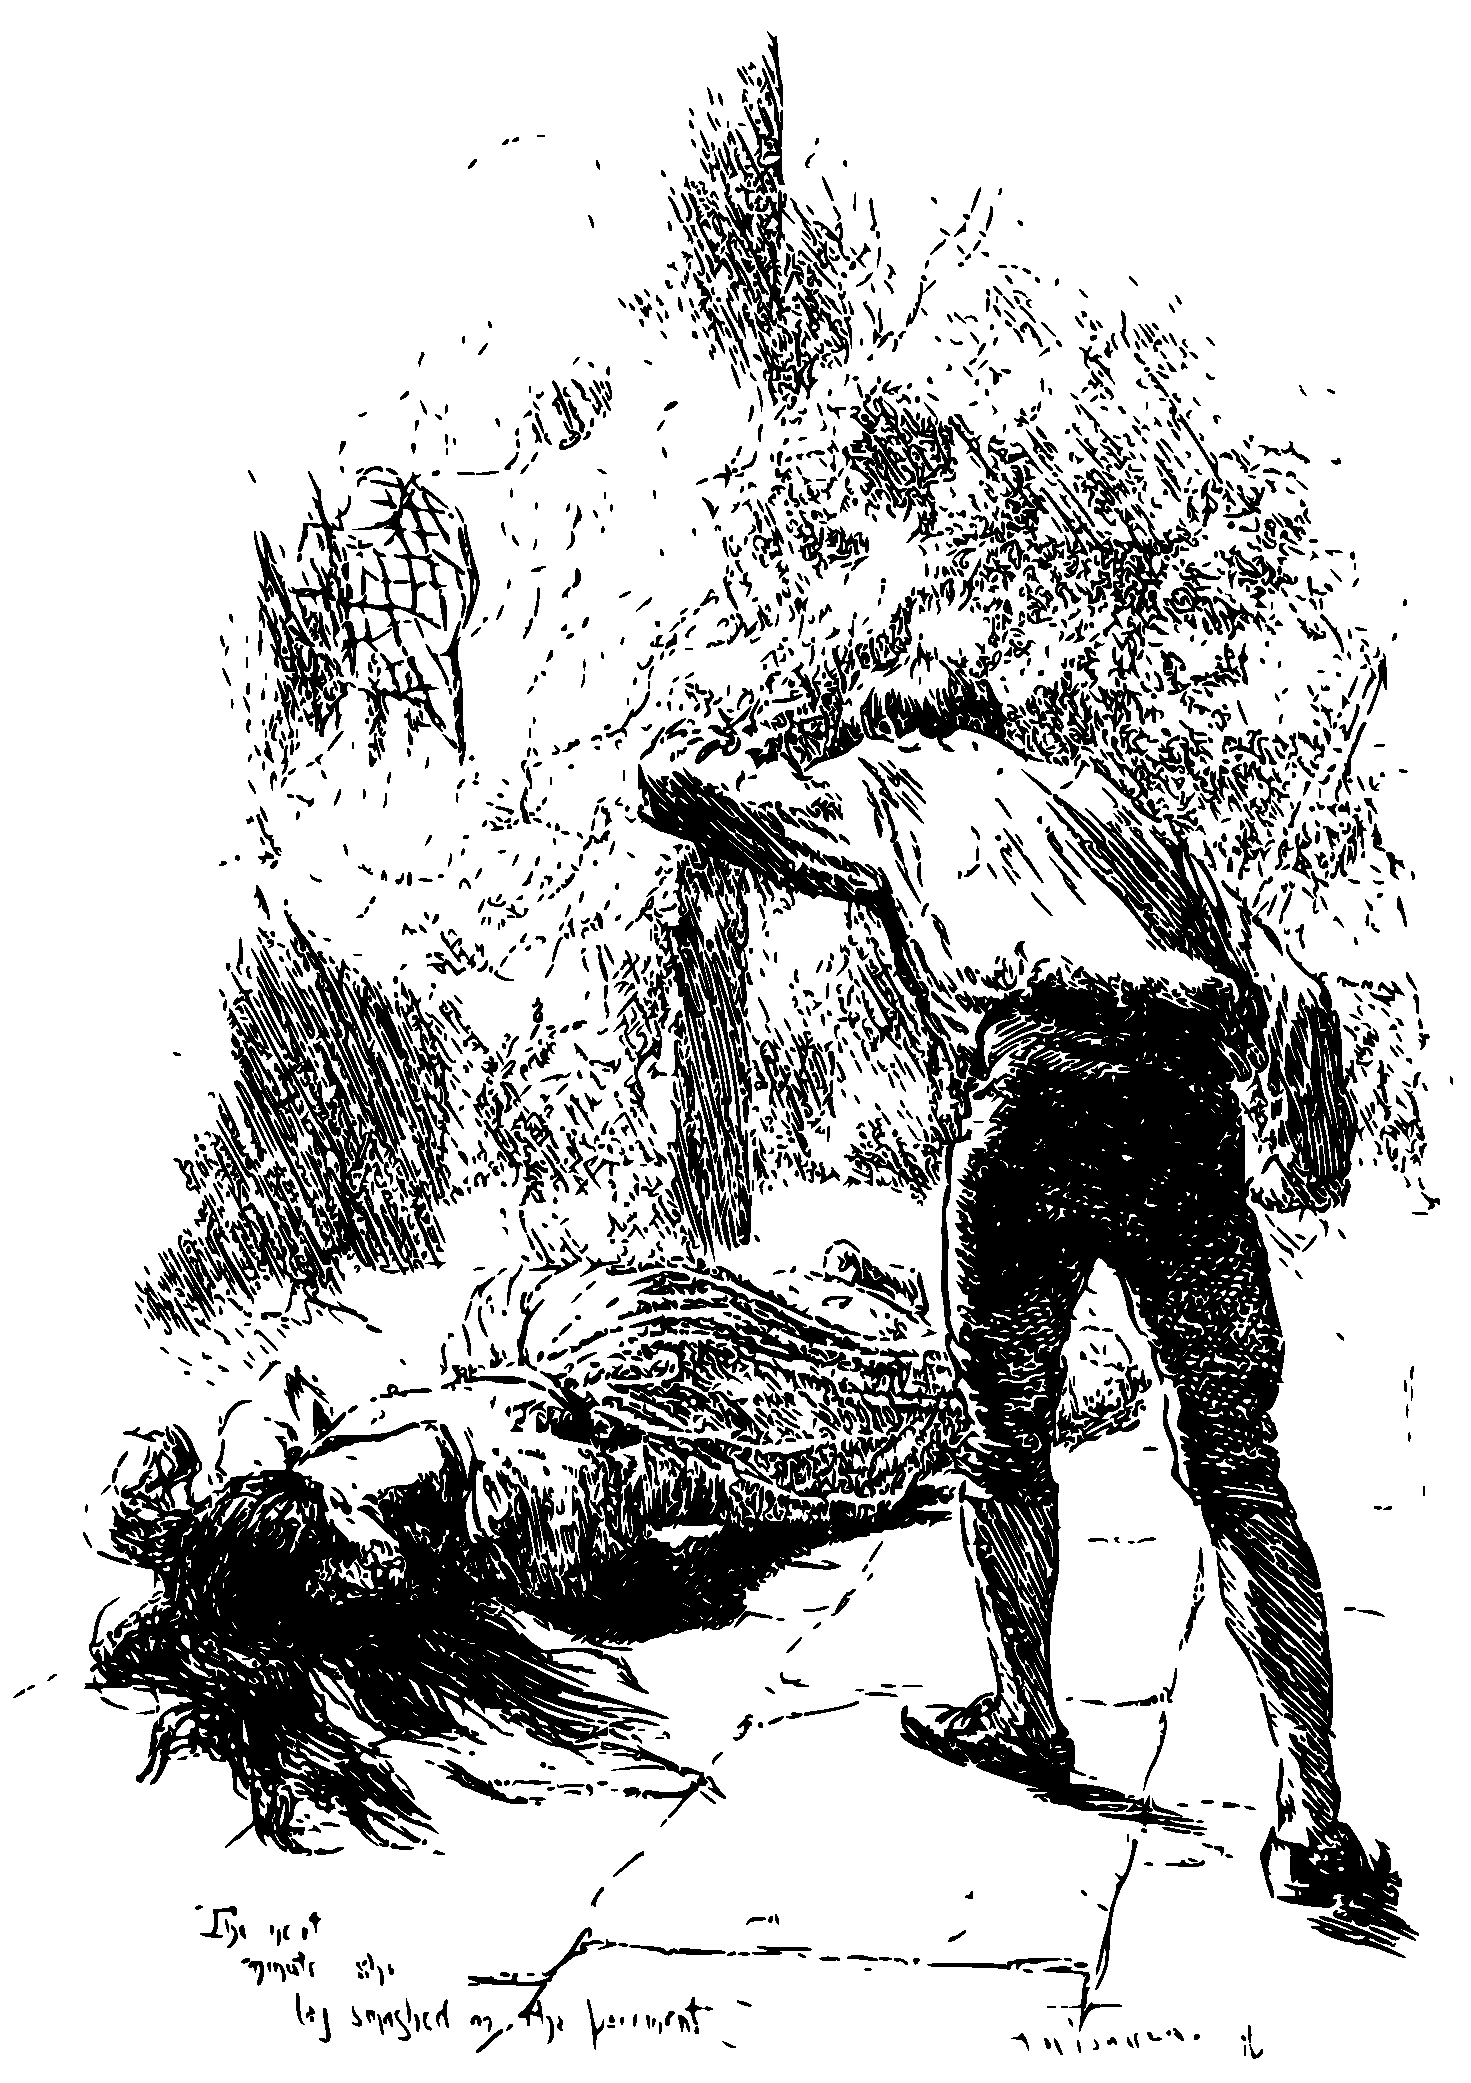
\includegraphics[width=\linewidth]{images/p413b.pdf}
	\end{sidecaption}
\end{figure}

\enquote{Dead?}

\enquote{Dead! Ay, dead as the stones on which her brains and blood
were scattered.}

\enquote{Good God!}

\enquote{You may well say so, ma'am: it was frightful!}

He shuddered.

\enquote{And afterwards?} I urged.

\enquote{Well, ma'am, afterwards the house was burnt to the ground:
there are only some bits of walls standing now.}

\enquote{Were any other lives lost?}

\enquote{No---perhaps it would have been better if there had.}

\enquote{What do you mean?}

\enquote{Poor \Mr{} Edward!} he ejaculated, \enquote{I little thought ever
to have seen it! Some say it was a just judgment on him for keeping his
first marriage secret, and wanting to take another wife while he had one
living: but I pity him, for my part.}

\enquote{You said he was alive?} I exclaimed.

\enquote{Yes, yes: he is alive; but many think he had better be dead.}

\enquote{Why? How?} My blood was again running cold. \enquote{Where
is he?} I demanded. \enquote{Is he in England?}

\enquote{Ay---ay---he's in England; he can't get out of England, I
fancy---he's a fixture now.}

What agony was this! And the man seemed resolved to protract it.

\enquote{He is stone-blind,} he said at last. \enquote{Yes, he is
stone-blind, is \Mr{} Edward.}

I had dreaded worse. I had dreaded he was mad. I summoned strength to
ask what had caused this calamity.

\enquote{It was all his own courage, and a body may say, his kindness,
in a way, ma'am: he wouldn't leave the house till every one else was out
before him. As he came down the great staircase at last, after \Mrs{}
 Rochester had flung herself from the battlements, there was a great
crash---all fell. He was taken out from under the ruins, alive, but
sadly hurt: a beam had fallen in such a way as to protect him partly;
but one eye was knocked out, and one hand so crushed that \Mr{} Carter,
the surgeon, had to amputate it directly. The other eye inflamed: he
lost the sight of that also. He is now helpless, indeed---blind and a
cripple.}

\enquote{Where is he? Where does he now live?}

\enquote{At Ferndean, a manor-house on a farm he has, about thirty miles
off: quite a desolate spot.}

\enquote{Who is with him?}

\enquote{Old John and his wife: he would have none else. He is quite
broken down, they say.}

\enquote{Have you any sort of conveyance?}

\enquote{We have a chaise, ma'am, a very handsome chaise.}

\enquote{Let it be got ready instantly; and if your post-boy can drive
me to Ferndean before dark this day, I'll pay both you and him twice the
hire you usually demand.}

\FChapter{Chapter Thirty-Seven}{37}

\Lettrine{T}{he} \textsc{manor-house} of Ferndean was a building of considerable antiquity,
moderate size, and no architectural pretensions, deep buried in a wood. 
I had heard of it before. \Mr{} Rochester often spoke of it, and
sometimes went there. His father had purchased the estate for the sake
of the game covers. He would have let the house, but could find no
tenant, in consequence of its ineligible and insalubrious site. 
Ferndean then remained uninhabited and unfurnished, with the exception
of some two or three rooms fitted up for the accommodation of the squire
when he went there in the season to shoot.

To this house I came just ere dark on an evening marked by the
characteristics of sad sky, cold gale, and continued small penetrating
rain. The last mile I performed on foot, having dismissed the chaise
and driver with the double remuneration I had promised. Even when
within a very short distance of the manor-house, you could see nothing
of it, so thick and dark grew the timber of the gloomy wood about it. 
Iron gates between granite pillars showed me where to enter, and passing
through them, I found myself at once in the twilight of close-ranked
trees. There was a grass-grown track descending the forest aisle
between hoar and knotty shafts and under branched arches. I followed
it, expecting soon to reach the dwelling; but it stretched on and on, it
wound far and farther: no sign of habitation or grounds was visible.

I thought I had taken a wrong direction and lost my way. The darkness
of natural as well as of sylvan dusk gathered over me. I looked round
in search of another road. There was none: all was interwoven stem,
columnar trunk, dense summer foliage---no opening anywhere.

I proceeded: at last my way opened, the trees thinned a little;
presently I beheld a railing, then the house---scarce, by this dim
light, distinguishable from the trees; so dank and green were its
decaying walls. Entering a portal, fastened only by a latch, I stood
amidst a space of enclosed ground, from which the wood swept away in a
semicircle. There were no flowers, no garden-beds; only a broad
gravel-walk girdling a grass-plat, and this set in the heavy frame of
the forest. The house presented two pointed gables in its front; the
windows were latticed and narrow: the front door was narrow too, one
step led up to it. The whole looked, as the host of the Rochester Arms
had said, \enquote{quite a desolate spot.} It was as still as a church
on a week-day: the pattering rain on the forest leaves was the only
sound audible in its vicinage.

\enquote{Can there be life here?} I asked.

Yes, life of some kind there was; for I heard a movement---that narrow
front-door was unclosing, and some shape was about to issue from the
grange.

It opened slowly: a figure came out into the twilight and stood on the
step; a man without a hat: he stretched forth his hand as if to feel
whether it rained. Dusk as it was, I had recognised him---it was my
master, Edward Fairfax Rochester, and no other.

I stayed my step, almost my breath, and stood to watch him---to examine
him, myself unseen, and alas! to him invisible. It was a sudden
meeting, and one in which rapture was kept well in check by pain. I had
no difficulty in restraining my voice from exclamation, my step from
hasty advance.

His form was of the same strong and stalwart contour as ever: his port
was still erect, his hair was still raven black; nor were his features
altered or sunk: not in one year's space, by any sorrow, could his
athletic strength be quelled or his vigorous prime blighted. But in his
countenance I saw a change: that looked desperate and brooding---that
reminded me of some wronged and fettered wild beast or bird, dangerous
to approach in his sullen woe. The caged eagle, whose gold-ringed eyes
cruelty has extinguished, might look as looked that sightless Samson.

And, reader, do you think I feared him in his blind ferocity?---if you
do, you little know me. A soft hope blest with my sorrow that soon I
should dare to drop a kiss on that brow of rock, and on those lips so
sternly sealed beneath it: but not yet. I would not accost him yet.

He descended the one step, and advanced slowly and gropingly towards the
grass-plat. Where was his daring stride now? Then he paused, as if he
knew not which way to turn. He lifted his hand and opened his eyelids;
gazed blank, and with a straining effort, on the sky, and toward the
amphitheatre of trees: one saw that all to him was void darkness. He
stretched his right hand (the left arm, the mutilated one, he kept
hidden in his bosom); he seemed to wish by touch to gain an idea of what
lay around him: he met but vacancy still; for the trees were some yards
off where he stood. He relinquished the endeavour, folded his arms, and
stood quiet and mute in the rain, now falling fast on his uncovered
head. At this moment John approached him from some quarter.

\enquote{Will you take my arm, sir?} he said; \enquote{there is a heavy
shower coming on: had you not better go in?}

\enquote{Let me alone,} was the answer.

John withdrew without having observed me. \Mr{} Rochester now tried to
walk about: vainly,---all was too uncertain. He groped his way back to
the house, and, re-entering it, closed the door.

I now drew near and knocked: John's wife opened for me. \enquote{Mary,}
I said, \enquote{how are you?}

She started as if she had seen a ghost: I calmed her. To her hurried
\enquote{Is it really you, miss, come at this late hour to this lonely
place?} I answered by taking her hand; and then I followed her into the
kitchen, where John now sat by a good fire. I explained to them, in few
words, that I had heard all which had happened since I left Thornfield,
and that I was come to see \Mr{} Rochester. I asked John to go down to
the turn-pike-house, where I had dismissed the chaise, and bring my
trunk, which I had left there: and then, while I removed my bonnet and
shawl, I questioned Mary as to whether I could be accommodated at the
Manor House for the night; and finding that arrangements to that effect,
though difficult, would not be impossible, I informed her I should
stay. Just at this moment the parlour-bell rang.

\enquote{When you go in,} said I, \enquote{tell your master that a
person wishes to speak to him, but do not give my name.}

\enquote{I don't think he will see you,} she answered; \enquote{he
refuses everybody.}

When she returned, I inquired what he had said. \enquote{You are to
send in your name and your business,} she replied. She then proceeded
to fill a glass with water, and place it on a tray, together with
candles.

\enquote{Is that what he rang for?} I asked.

\enquote{Yes: he always has candles brought in at dark, though he is
blind.}

\enquote{Give the tray to me; I will carry it in.}

I took it from her hand: she pointed me out the parlour door. The tray
shook as I held it; the water spilt from the glass; my heart struck my
ribs loud and fast. Mary opened the door for me, and shut it behind me.

This parlour looked gloomy: a neglected handful of fire burnt low in the
grate; and, leaning over it, with his head supported against the high,
old-fashioned mantelpiece, appeared the blind tenant of the room. His
old dog, Pilot, lay on one side, removed out of the way, and coiled up
as if afraid of being inadvertently trodden upon. Pilot pricked up his
ears when I came in: then he jumped up with a yelp and a whine, and
bounded towards me: he almost knocked the tray from my hands. I set it
on the table; then patted him, and said softly, \enquote{Lie down!} \Mr{}
 Rochester turned mechanically to \emph{see} what the commotion was: but
as he \emph{saw} nothing, he returned and sighed.

\enquote{Give me the water, Mary,} he said.

I approached him with the now only half-filled glass; Pilot followed me,
still excited.

\enquote{What is the matter?} he inquired.

\enquote{Down, Pilot!} I again said. He checked the water on its way to
his lips, and seemed to listen: he drank, and put the glass down. 
\enquote{This is you, Mary, is it not?}

\enquote{Mary is in the kitchen,} I answered.

He put out his hand with a quick gesture, but not seeing where I stood,
he did not touch me. \enquote{Who is this? Who is this?} he demanded,
trying, as it seemed, to \emph{see} with those sightless
eyes---unavailing and distressing attempt! \enquote{Answer me---speak
again!} he ordered, imperiously and aloud.

\enquote{Will you have a little more water, sir? I spilt half of what
was in the glass,} I said.

\enquote{\emph{Who} is it? \emph{What} is it? Who speaks?}

\enquote{Pilot knows me, and John and Mary know I am here. I came only
this evening,} I answered.

\enquote{Great God!---what delusion has come over me? What sweet
madness has seized me?}

\enquote{No delusion---no madness: your mind, sir, is too strong for
delusion, your health too sound for frenzy.}

\enquote{And where is the speaker? Is it only a voice? Oh! I \emph{cannot}
see, but I must feel, or my heart will stop and my brain burst. 
Whatever---whoever you are---be perceptible to the touch or I cannot
live!}

He groped; I arrested his wandering hand, and prisoned it in both mine.

\enquote{Her very fingers!} he cried; \enquote{her small, slight
fingers! If so there must be more of her.}

The muscular hand broke from my custody; my arm was seized, my
shoulder---neck---waist---I was entwined and gathered to him.

\enquote{Is it Jane? \emph{What} is it? This is her shape---this is her
size---}

\enquote{And this her voice,} I added. \enquote{She is all here: her
heart, too. God bless you, sir! I am glad to be so near you again.}

\enquote{Jane Eyre!---Jane Eyre,} was all he said.

\enquote{My dear master,} I answered, \enquote{I am Jane Eyre: I have
found you out---I am come back to you.}

\enquote{In truth?---in the flesh? My living Jane?}

\enquote{You touch me, sir,---you hold me, and fast enough: I am not
cold like a corpse, nor vacant like air, am I?}

\enquote{My living darling! These are certainly her limbs, and these
her features; but I cannot be so blest, after all my misery. It is a
dream; such dreams as I have had at night when I have clasped her once
more to my heart, as I do now; and kissed her, as thus---and felt that
she loved me, and trusted that she would not leave me.}

\enquote{Which I never will, sir, from this day.}

\enquote{Never will, says the vision? But I always woke and found it an
empty mockery; and I was desolate and abandoned---my life dark, lonely,
hopeless---my soul athirst and forbidden to drink---my heart famished
and never to be fed. Gentle, soft dream, nestling in my arms now, you
will fly, too, as your sisters have all fled before you: but kiss me
before you go---embrace me, Jane.}

\enquote{There, sir---and there!}'

I pressed my lips to his once brilliant and now rayless eyes---I swept
his hair from his brow, and kissed that too. He suddenly seemed to
arouse himself: the conviction of the reality of all this seized him.

\enquote{It is you---is it, Jane? You are come back to me then?}

\enquote{I am.}

\enquote{And you do not lie dead in some ditch under some stream? And
you are not a pining outcast amongst strangers?}

\enquote{No, sir! I am an independent woman now.}

\enquote{Independent! What do you mean, Jane?}

\enquote{My uncle in Madeira is dead, and he left me five thousand
pounds.}

\enquote{Ah! this is practical---this is real!} he cried: \enquote{I
should never dream that. Besides, there is that peculiar voice of hers,
so animating and piquant, as well as soft: it cheers my withered heart;
it puts life into it.---What, Janet! Are you an independent woman? A
rich woman?}

\enquote{If you won't let me live with you, I can build a house of my
own close up to your door, and you may come and sit in my parlour when
you want company of an evening.}

\enquote{But as you are rich, Jane, you have now, no doubt, friends who
will look after you, and not suffer you to devote yourself to a blind
lameter like me?}

\enquote{I told you I am independent, sir, as well as rich: I am my own
mistress.}

\enquote{And you will stay with me?}

\enquote{Certainly---unless you object. I will be your neighbour, your
nurse, your housekeeper. I find you lonely: I will be your
companion---to read to you, to walk with you, to sit with you, to wait
on you, to be eyes and hands to you. Cease to look so melancholy, my
dear master; you shall not be left desolate, so long as I live.}

He replied not: he seemed serious---abstracted; he sighed; he
half-opened his lips as if to speak: he closed them again. I felt a
little embarrassed. Perhaps I had too rashly over-leaped
conventionalities; and he, like \St{} John, saw impropriety in my
inconsiderateness. I had indeed made my proposal from the idea that he
wished and would ask me to be his wife: an expectation, not the less
certain because unexpressed, had buoyed me up, that he would claim me at
once as his own. But no hint to that effect escaping him and his
countenance becoming more overcast, I suddenly remembered that I might
have been all wrong, and was perhaps playing the fool unwittingly; and I
began gently to withdraw myself from his arms---but he eagerly snatched
me closer.

\enquote{No---no---Jane; you must not go. No---I have touched you,
heard you, felt the comfort of your presence---the sweetness of your
consolation: I cannot give up these joys. I have little left in
myself---I must have you. The world may laugh---may call me absurd,
selfish---but it does not signify. My very soul demands you: it will be
satisfied, or it will take deadly vengeance on its frame.}

\enquote{Well, sir, I will stay with you: I have said so.}

\enquote{Yes---but you understand one thing by staying with me; and I
understand another. You, perhaps, could make up your mind to be about
my hand and chair---to wait on me as a kind little nurse (for you have
an affectionate heart and a generous spirit, which prompt you to make
sacrifices for those you pity), and that ought to suffice for me no
doubt. I suppose I should now entertain none but fatherly feelings for
you: do you think so? Come---tell me.}

\enquote{I will think what you like, sir: I am content to be only your
nurse, if you think it better.}

\enquote{But you cannot always be my nurse, Janet: you are young---you
must marry one day.}

\enquote{I don't care about being married.}

\enquote{You should care, Janet: if I were what I once was, I would try
to make you care---but---a sightless block!}

He relapsed again into gloom. I, on the contrary, became more cheerful,
and took fresh courage: these last words gave me an insight as to where
the difficulty lay; and as it was no difficulty with me, I felt quite
relieved from my previous embarrassment. I resumed a livelier vein of
conversation.

\enquote{It is time some one undertook to rehumanise you,} said I,
parting his thick and long uncut locks; \enquote{for I see you are being
metamorphosed into a lion, or something of that sort. You have a
\enquote{faux air} of Nebuchadnezzar in the fields about you, that is
certain: your hair reminds me of eagles' feathers; whether your nails
are grown like birds' claws or not, I have not yet noticed.}

\enquote{On this arm, I have neither hand nor nails,} he said, drawing
the mutilated limb from his breast, and showing it to me. \enquote{It
is a mere stump---a ghastly sight! Don't you think so, Jane?}

\enquote{It is a pity to see it; and a pity to see your eyes---and the
scar of fire on your forehead: and the worst of it is, one is in danger
of loving you too well for all this; and making too much of you.}

\enquote{I thought you would be revolted, Jane, when you saw my arm, and
my cicatrised visage.}

\enquote{Did you? Don't tell me so---lest I should say something
disparaging to your judgment. Now, let me leave you an instant, to make
a better fire, and have the hearth swept up. Can you tell when there is
a good fire?}

\enquote{Yes; with the right eye I see a glow---a ruddy haze.}

\enquote{And you see the candles?}

\enquote{Very dimly---each is a luminous cloud.}

\enquote{Can you see me?}

\enquote{No, my fairy: but I am only too thankful to hear and feel you.}

\enquote{When do you take supper?}

\enquote{I never take supper.}

\enquote{But you shall have some to-night. I am hungry: so are you, I
daresay, only you forget.}

Summoning Mary, I soon had the room in more cheerful order: I prepared
him, likewise, a comfortable repast. My spirits were excited, and with
pleasure and ease I talked to him during supper, and for a long time
after. There was no harassing restraint, no repressing of glee and
vivacity with him; for with him I was at perfect ease, because I knew I
suited him; all I said or did seemed either to console or revive him. 
Delightful consciousness! It brought to life and light my whole nature:
in his presence I thoroughly lived; and he lived in mine. Blind as he
was, smiles played over his face, joy dawned on his forehead: his
lineaments softened and warmed.

After supper, he began to ask me many questions, of where I had been,
what I had been doing, how I had found him out; but I gave him only very
partial replies: it was too late to enter into particulars that night. 
Besides, I wished to touch no deep-thrilling chord---to open no fresh
well of emotion in his heart: my sole present aim was to cheer him. 
Cheered, as I have said, he was: and yet but by fits. If a moment's
silence broke the conversation, he would turn restless, touch me, then
say, \enquote{Jane.}

\enquote{You are altogether a human being, Jane? You are certain of
that?}

\begin{figure}
	\begin{sidecaption}{\enquote{You are altogether a\linebreak human being, Jane?\linebreak You are certain of that?}}[p422b]
		\centering
		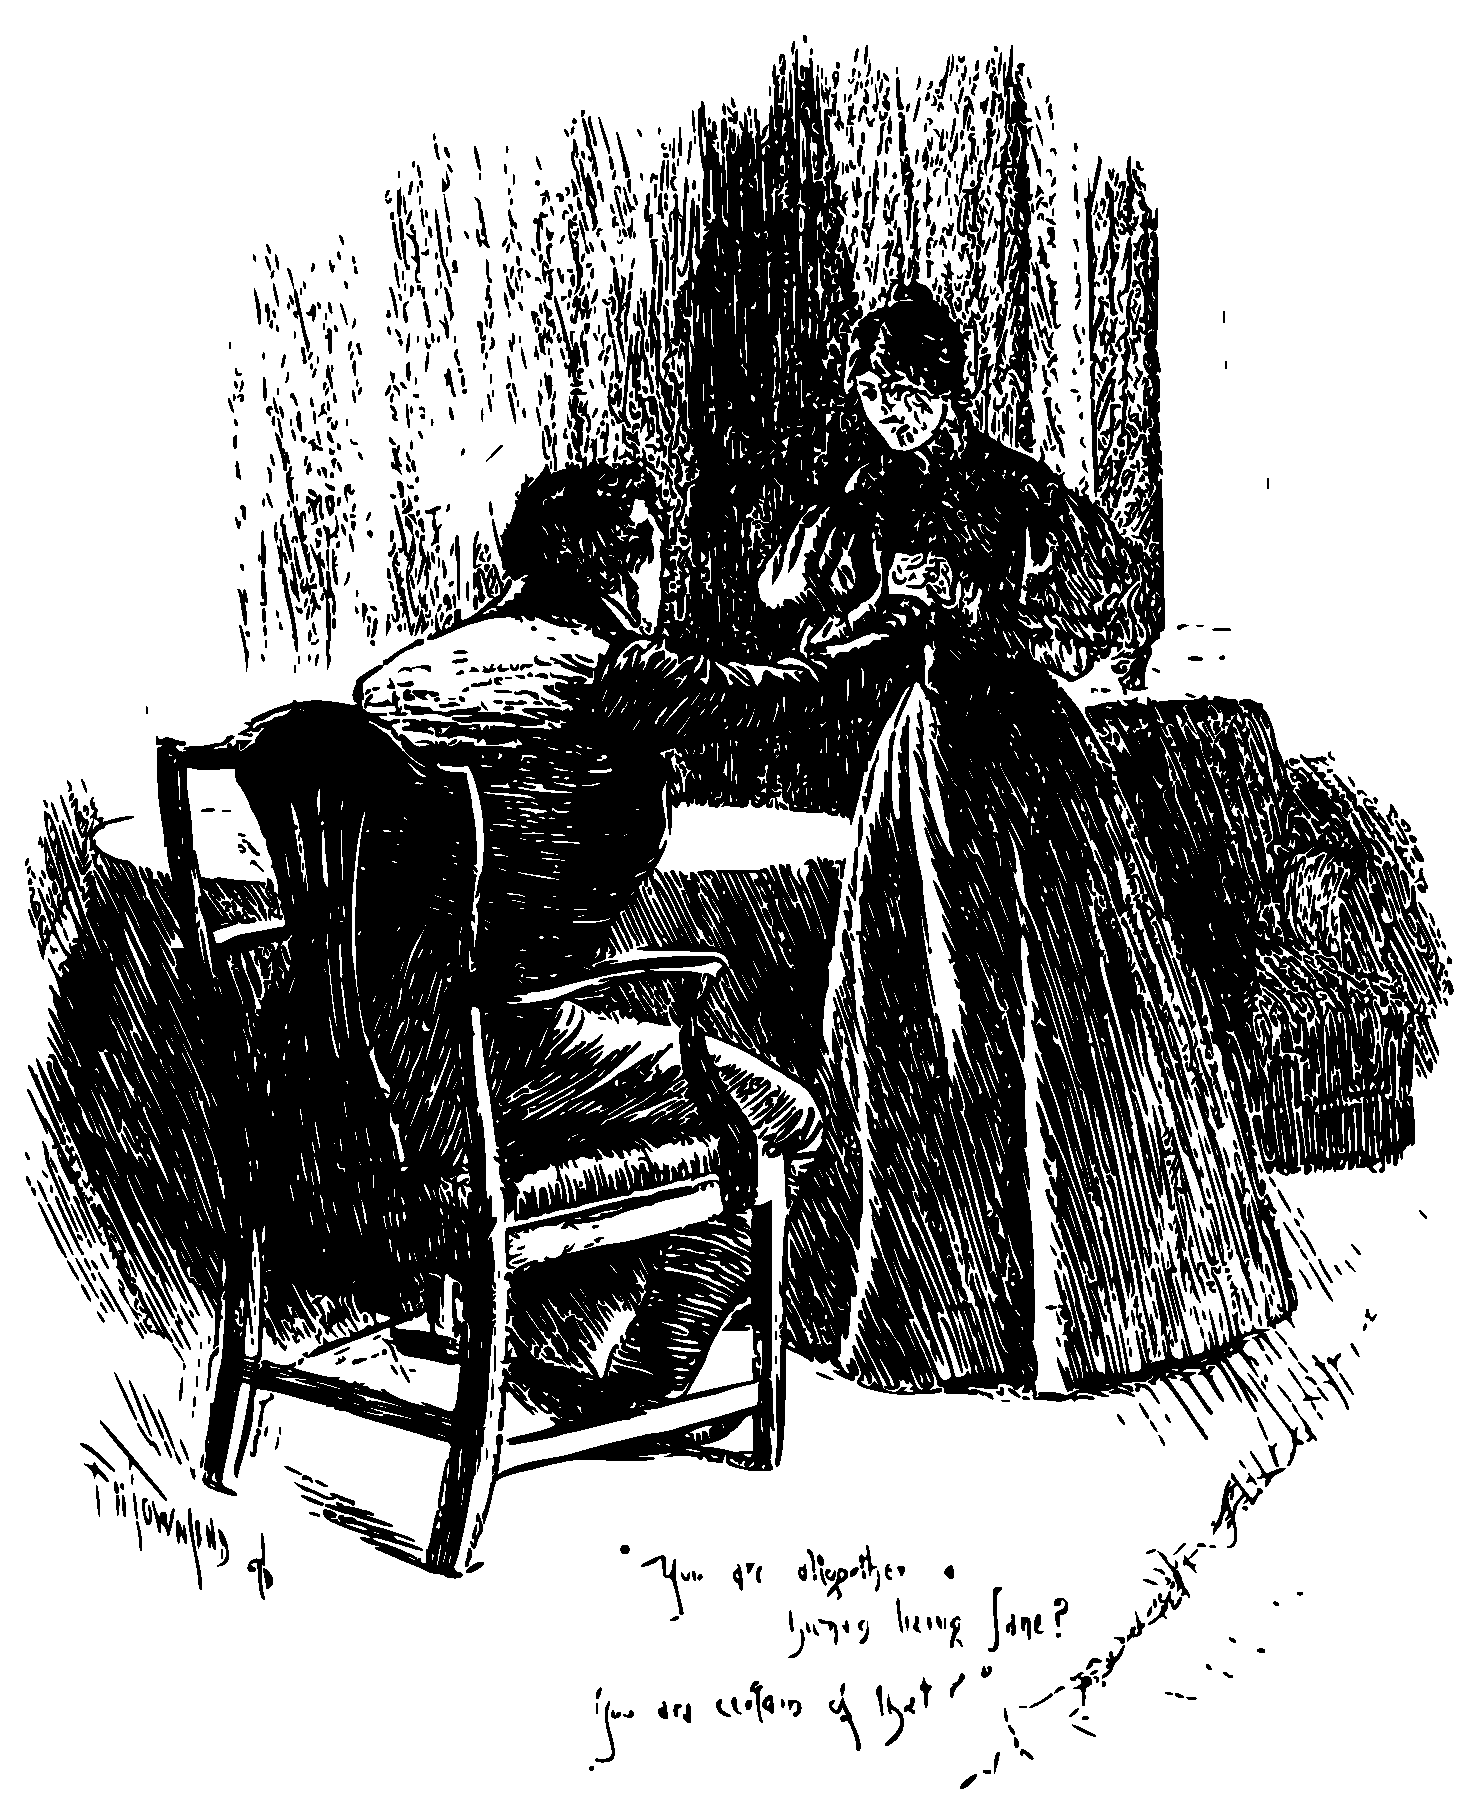
\includegraphics[width=\linewidth]{images/p422b.pdf}
	\end{sidecaption}
\end{figure}

\enquote{I conscientiously believe so, \Mr{} Rochester.}

\enquote{Yet how, on this dark and doleful evening, could you so
suddenly rise on my lone hearth? I stretched my hand to take a glass of
water from a hireling, and it was given me by you: I asked a question,
expecting John's wife to answer me, and your voice spoke at my ear.}

\enquote{Because I had come in, in Mary's stead, with the tray.}

\enquote{And there is enchantment in the very hour I am now spending
with you. Who can tell what a dark, dreary, hopeless life I have
dragged on for months past? Doing nothing, expecting nothing; merging
night in day; feeling but the sensation of cold when I let the fire go
out, of hunger when I forgot to eat: and then a ceaseless sorrow, and,
at times, a very delirium of desire to behold my Jane again. Yes: for
her restoration I longed, far more than for that of my lost sight. How
can it be that Jane is with me, and says she loves me? Will she not
depart as suddenly as she came? To-morrow, I fear I shall find her no
more.}

A commonplace, practical reply, out of the train of his own disturbed
ideas, was, I was sure, the best and most reassuring for him in this
frame of mind. I passed my finger over his eyebrows, and remarked that
they were scorched, and that I would apply something which would make
them grow as broad and black as ever.

\enquote{Where is the use of doing me good in any way, beneficent spirit, when,
at some fatal moment, you will again desert me---passing like a shadow,
whither and how to me unknown, and for me remaining afterwards
undiscoverable?} %fix missing end quote

\enquote{Have you a pocket-comb about you, sir?}

\enquote{What for, Jane?}

\enquote{Just to comb out this shaggy black mane. I find you rather
alarming, when I examine you close at hand: you talk of my being a
fairy, but I am sure, you are more like a brownie.}

\enquote{Am I hideous, Jane?}

\enquote{Very, sir: you always were, you know.}

\enquote{Humph! The wickedness has not been taken out of you, wherever
you have sojourned.}

\enquote{Yet I have been with good people; far better than you: a
hundred times better people; possessed of ideas and views you never
entertained in your life: quite more refined and exalted.}

\enquote{Who the deuce have you been with?}

\enquote{If you twist in that way you will make me pull the hair out of
your head; and then I think you will cease to entertain doubts of my
substantiality.}

\enquote{Who have you been with, Jane?}

\enquote{You shall not get it out of me to-night, sir; you must wait
till to-morrow; to leave my tale half told, will, you know, be a sort of
security that I shall appear at your breakfast table to finish it. By
the bye, I must mind not to rise on your hearth with only a glass of
water then: I must bring an egg at the least, to say nothing of fried
ham.}

\enquote{You mocking changeling---fairy-born and human-bred! You make
me feel as I have not felt these twelve months. If Saul could have had
you for his David, the evil spirit would have been exorcised without the
aid of the harp.}

\enquote{There, sir, you are redd up and made decent. Now I'll leave
you: I have been travelling these last three days, and I believe I am
tired. Good night.}

\enquote{Just one word, Jane: were there only ladies in the house where
you have been?}

I laughed and made my escape, still laughing as I ran upstairs. 
\enquote{A good idea!} I thought with glee. \enquote{I see I have the
means of fretting him out of his melancholy for some time to come.}

Very early the next morning I heard him up and astir, wandering from one
room to another. As soon as Mary came down I heard the question:
\enquote{Is Miss Eyre here?} Then: \enquote{Which room did you put her
into? Was it dry? Is she up? Go and ask if she wants anything; and
when she will come down.}

I came down as soon as I thought there was a prospect of breakfast. 
Entering the room very softly, I had a view of him before he discovered
my presence. It was mournful, indeed, to witness the subjugation of
that vigorous spirit to a corporeal infirmity. He sat in his
chair---still, but not at rest: expectant evidently; the lines of now
habitual sadness marking his strong features. His countenance reminded
one of a lamp quenched, waiting to be re-lit---and alas! it was not
himself that could now kindle the lustre of animated expression: he was
dependent on another for that office! I had meant to be gay and
careless, but the powerlessness of the strong man touched my heart to
the quick: still I accosted him with what vivacity I could.

\enquote{It is a bright, sunny morning, sir,} I said. \enquote{The rain
is over and gone, and there is a tender shining after it: you shall have
a walk soon.}

I had wakened the glow: his features beamed.

\enquote{Oh, you are indeed there, my skylark! Come to me. You are not
gone: not vanished? I heard one of your kind an hour ago, singing high
over the wood: but its song had no music for me, any more than the
rising sun had rays. All the melody on earth is concentrated in my
Jane's tongue to my ear (I am glad it is not naturally a silent one):
all the sunshine I can feel is in her presence.}

The water stood in my eyes to hear this avowal of his dependence; just
as if a royal eagle, chained to a perch, should be forced to entreat a
sparrow to become its purveyor. But I would not be lachrymose: I dashed
off the salt drops, and busied myself with preparing breakfast.

Most of the morning was spent in the open air. I led him out of the wet
and wild wood into some cheerful fields: I described to him how
brilliantly green they were; how the flowers and hedges looked
refreshed; how sparklingly blue was the sky. I sought a seat for him in
a hidden and lovely spot, a dry stump of a tree; nor did I refuse to let
him, when seated, place me on his knee. Why should I, when both he and
I were happier near than apart? Pilot lay beside us: all was quiet. He
broke out suddenly while clasping me in his arms---

\enquote{Cruel, cruel deserter! Oh, Jane, what did I feel when I
discovered you had fled from Thornfield, and when I could nowhere find
you; and, after examining your apartment, ascertained that you had taken
no money, nor anything which could serve as an equivalent! A pearl
necklace I had given you lay untouched in its little casket; your trunks
were left corded and locked as they had been prepared for the bridal
tour. What could my darling do, I asked, left destitute and penniless? 
And what did she do? Let me hear now.}

Thus urged, I began the narrative of my experience for the last year. I
softened considerably what related to the three days of wandering and
starvation, because to have told him all would have been to inflict
unnecessary pain: the little I did say lacerated his faithful heart
deeper than I wished.

I should not have left him thus, he said, without any means of making my
way: I should have told him my intention. I should have confided in
him: he would never have forced me to be his mistress. Violent as he
had seemed in his despair, he, in truth, loved me far too well and too
tenderly to constitute himself my tyrant: he would have given me half
his fortune, without demanding so much as a kiss in return, rather than
I should have flung myself friendless on the wide world. I had endured,
he was certain, more than I had confessed to him.

\enquote{Well, whatever my sufferings had been, they were very short,} I
answered: and then I proceeded to tell him how I had been received at
Moor House; how I had obtained the office of schoolmistress, \etc. The
accession of fortune, the discovery of my relations, followed in due
order. Of course, \St{} John Rivers' name came in frequently in the
progress of my tale. When I had done, that name was immediately taken
up.

\enquote{This \St{} John, then, is your cousin?}

\enquote{Yes.}

\enquote{You have spoken of him often: do you like him?}

\enquote{He was a very good man, sir; I could not help liking him.}

\enquote{A good man. Does that mean a respectable well-conducted man of
fifty? Or what does it mean?}

\enquote{St John was only twenty-nine, sir.}

\enquote{\foreignquote{french}{\emph{Jeune encore,}}\footnote{young again} as the French say. Is he a person of low
stature, phlegmatic, and plain. A person whose goodness consists rather
in his guiltlessness of vice, than in his prowess in virtue.}

\enquote{He is untiringly active. Great and exalted deeds are what he
lives to perform.}

\enquote{But his brain? That is probably rather soft? He means well:
but you shrug your shoulders to hear him talk?}

\enquote{He talks little, sir: what he does say is ever to the point. 
His brain is first-rate, I should think not impressible, but vigorous.}

\enquote{Is he an able man, then?}

\enquote{Truly able.}

\enquote{A thoroughly educated man?}

\enquote{\St{} John is an accomplished and profound scholar.}

\enquote{His manners, I think, you said are not to your
taste?---priggish and parsonic?}

\enquote{I never mentioned his manners; but, unless I had a very bad
taste, they must suit it; they are polished, calm, and gentlemanlike.}

\enquote{His appearance,---I forget what description you gave of his
appearance;---a sort of raw curate, half strangled with his white
neckcloth, and stilted up on his thick-soled high-lows, eh?}

\enquote{\St{} John dresses well. He is a handsome man: tall, fair, with
blue eyes, and a Grecian profile.}

(Aside.) \enquote{Damn him!}---(To me.) \enquote{Did you like him,
Jane?}

\enquote{Yes, \Mr{} Rochester, I liked him: but you asked me that before.}

I perceived, of course, the drift of my interlocutor. Jealousy had got
hold of him: she stung him; but the sting was salutary: it gave him
respite from the gnawing fang of melancholy. I would not, therefore,
immediately charm the snake.

\enquote{Perhaps you would rather not sit any longer on my knee, Miss
Eyre?} was the next somewhat unexpected observation.

\enquote{Why not, \Mr{} Rochester?}

\enquote{The picture you have just drawn is suggestive of a rather too
overwhelming contrast. Your words have delineated very prettily a
graceful Apollo: he is present to your imagination,---tall, fair,
blue-eyed, and with a Grecian profile. Your eyes dwell on a Vulcan,---a
real blacksmith, brown, broad-shouldered: and blind and lame into the
bargain.}

\enquote{I never thought of it, before; but you certainly are rather
like Vulcan, sir.}

\enquote{Well, you can leave me, ma'am: but before you go} (and he
retained me by a firmer grasp than ever), \enquote{you will be pleased
just to answer me a question or two.} He paused.

\enquote{What questions, \Mr{} Rochester?}

Then followed this cross-examination.

\enquote{\St{} John made you schoolmistress of Morton before he knew you
were his cousin?}

\enquote{Yes.}

\enquote{You would often see him? He would visit the school sometimes?}

\enquote{Daily.}

\enquote{He would approve of your plans, Jane? I know they would be
clever, for you are a talented creature!}

\enquote{He approved of them---yes.}

\enquote{He would discover many things in you he could not have expected
to find? Some of your accomplishments are not ordinary.}

\enquote{I don't know about that.}

\enquote{You had a little cottage near the school, you say: did he ever
come there to see you?}

\enquote{Now and then?}

\enquote{Of an evening?}

\enquote{Once or twice.}

A pause.

\enquote{How long did you reside with him and his sisters after the
cousinship was discovered?}

\enquote{Five months.}

\enquote{Did Rivers spend much time with the ladies of his family?}

\enquote{Yes; the back parlour was both his study and ours: he sat near
the window, and we by the table.}

\enquote{Did he study much?}

\enquote{A good deal.}

\enquote{What?}

\enquote{Hindostanee.}

\enquote{And what did you do meantime?}

\enquote{I learnt German, at first.}

\enquote{Did he teach you?}

\enquote{He did not understand German.}

\enquote{Did he teach you nothing?}

\enquote{A little Hindostanee.}

\enquote{Rivers taught you Hindostanee?}

\enquote{Yes, sir.}

\enquote{And his sisters also?}

\enquote{No.}

\enquote{Only you?}

\enquote{Only me.}

\enquote{Did you ask to learn?}

\enquote{No.}

\enquote{He wished to teach you?}

\enquote{Yes.}

A second pause.

\enquote{Why did he wish it? Of what use could Hindostanee be to you?}

\enquote{He intended me to go with him to India.}

\enquote{Ah! here I reach the root of the matter. He wanted you to
marry him?}

\enquote{He asked me to marry him.}

\enquote{That is a fiction---an impudent invention to vex me.}

\enquote{I beg your pardon, it is the literal truth: he asked me more
than once, and was as stiff about urging his point as ever you could
be.}

\enquote{Miss Eyre, I repeat it, you can leave me. How often am I to
say the same thing? Why do you remain pertinaciously perched on my
knee, when I have given you notice to quit?}

\enquote{Because I am comfortable there.}

\enquote{No, Jane, you are not comfortable there, because your heart is
not with me: it is with this cousin---this \St{} John. Oh, till this
moment, I thought my little Jane was all mine! I had a belief she loved
me even when she left me: that was an atom of sweet in much bitter. 
Long as we have been parted, hot tears as I have wept over our
separation, I never thought that while I was mourning her, she was
loving another! But it is useless grieving. Jane, leave me: go and
marry Rivers.}

\enquote{Shake me off, then, sir,---push me away, for I'll not leave you
of my own accord.}

\enquote{Jane, I ever like your tone of voice: it still renews hope, it
sounds so truthful. When I hear it, it carries me back a year. I
forget that you have formed a new tie. But I am not a fool---go---}

\enquote{Where must I go, sir?}

\enquote{Your own way---with the husband you have chosen.}

\enquote{Who is that?}

\enquote{You know---this \St{} John Rivers.}

\enquote{He is not my husband, nor ever will be. He does not love me: I do not
love him. He loves (as he \emph{can} love, and that is not as you love)
a beautiful young lady called Rosamond. He wanted to marry me only
because he thought I should make a suitable missionary's wife, which she
would not have done. He is good and great, but severe; and, for me,
cold as an iceberg. He is not like you, sir: I am not happy at his
side, nor near him, nor with him. He has no indulgence for me---no
fondness. He sees nothing attractive in me; not even youth---only a few
useful mental points.---Then I must leave you, sir, to go to him?}

I shuddered involuntarily, and clung instinctively closer to my blind
but beloved master. He smiled.

\enquote{What, Jane! Is this true? Is such really the state of matters
between you and Rivers?}

\enquote{Absolutely, sir! Oh, you need not be jealous! I wanted to tease you
a little to make you less sad: I thought anger would be better than
grief. But if you wish me to love you, could you but see how much I
\emph{do} love you, you would be proud and content. All my heart is
yours, sir: it belongs to you; and with you it would remain, were fate
to exile the rest of me from your presence for ever.}

Again, as he kissed me, painful thoughts darkened his aspect.

\enquote{My seared vision! My crippled strength!} he murmured
regretfully.

I caressed, in order to soothe him. I knew of what he was thinking, and
wanted to speak for him, but dared not. As he turned aside his face a
minute, I saw a tear slide from under the sealed eyelid, and trickle
down the manly cheek. My heart swelled.

\enquote{I am no better than the old lightning-struck chestnut-tree in
Thornfield orchard,} he remarked ere long. \enquote{And what right
would that ruin have to bid a budding woodbine cover its decay with
freshness?}

\enquote{You are no ruin, sir---no lightning-struck tree: you are green
and vigorous. Plants will grow about your roots, whether you ask them
or not, because they take delight in your bountiful shadow; and as they
grow they will lean towards you, and wind round you, because your
strength offers them so safe a prop.}

Again he smiled: I gave him comfort.

\enquote{You speak of friends, Jane?} he asked.

\enquote{Yes, of friends,} I answered rather hesitatingly: for I knew I
meant more than friends, but could not tell what other word to employ. 
He helped me.

\enquote{Ah! Jane. But I want a wife.}

\enquote{Do you, sir?}

\enquote{Yes: is it news to you?}

\enquote{Of course: you said nothing about it before.}

\enquote{Is it unwelcome news?}

\enquote{That depends on circumstances, sir---on your choice.}

\enquote{Which you shall make for me, Jane. I will abide by your
decision.}

\enquote{Choose then, sir---\emph{her who loves you best}.}

\enquote{I will at least choose---\emph{her I love best}. Jane, will you marry
me?}

\enquote{Yes, sir.}

\enquote{A poor blind man, whom you will have to lead about by the
hand?}

\enquote{Yes, sir.}

\enquote{A crippled man, twenty years older than you, whom you will have
to wait on?}

\enquote{Yes, sir.}

\enquote{Truly, Jane?}

\enquote{Most truly, sir.}

\enquote{Oh! my darling! God bless you and reward you!}

\enquote{\Mr{} Rochester, if ever I did a good deed in my life---if ever I
thought a good thought---if ever I prayed a sincere and blameless
prayer---if ever I wished a righteous wish,---I am rewarded now. To be
your wife is, for me, to be as happy as I can be on earth.}

\enquote{Because you delight in sacrifice.}

\enquote{Sacrifice! What do I sacrifice? Famine for food, expectation
for content. To be privileged to put my arms round what I value---to
press my lips to what I love---to repose on what I trust: is that to
make a sacrifice? If so, then certainly I delight in sacrifice.}

\enquote{And to bear with my infirmities, Jane: to overlook my
deficiencies.}

\enquote{Which are none, sir, to me. I love you better now, when I can
really be useful to you, than I did in your state of proud independence,
when you disdained every part but that of the giver and protector.}

\enquote{Hitherto I have hated to be helped---to be led: henceforth, I
feel I shall hate it no more. I did not like to put my hand into a
hireling's, but it is pleasant to feel it circled by Jane's little
fingers. I preferred utter loneliness to the constant attendance of
servants; but Jane's soft ministry will be a perpetual joy. Jane suits
me: do I suit her?}

\enquote{To the finest fibre of my nature, sir.}

\enquote{The case being so, we have nothing in the world to wait for: we
must be married instantly.}

He looked and spoke with eagerness: his old impetuosity was rising.

\enquote{We must become one flesh without any delay, Jane: there is but
the licence to get---then we marry.}

\enquote{\Mr{} Rochester, I have just discovered the sun is far declined
from its meridian, and Pilot is actually gone home to his dinner. Let
me look at your watch.}

\enquote{Fasten it into your girdle, Janet, and keep it henceforward: I
have no use for it.}

\enquote{It is nearly four o'clock in the afternoon, sir. Don't you
feel hungry?}

\enquote{The third day from this must be our wedding-day, Jane. Never
mind fine clothes and jewels, now: all that is not worth a fillip.}

\enquote{The sun has dried up all the rain-drops, sir. The breeze is
still: it is quite hot.}

\enquote{Do you know, Jane, I have your little pearl necklace at this
moment fastened round my bronze scrag under my cravat? I have worn it
since the day I lost my only treasure, as a memento of her.}

\enquote{We will go home through the wood: that will be the shadiest
way.}

He pursued his own thoughts without heeding me.

\enquote{Jane! you think me, I daresay, an irreligious dog: but my heart swells
with gratitude to the beneficent God of this earth just now. He sees
not as man sees, but far clearer: judges not as man judges, but far more
wisely. I did wrong: I would have sullied my innocent flower---breathed
guilt on its purity: the Omnipotent snatched it from me. I, in my
stiff-necked rebellion, almost cursed the dispensation: instead of
bending to the decree, I defied it. Divine justice pursued its course;
disasters came thick on me: I was forced to pass through the valley of
the shadow of death. \emph{His} chastisements are mighty; and one smote
me which has humbled me for ever. You know I was proud of my strength:
but what is it now, when I must give it over to foreign guidance, as a
child does its weakness? Of late, Jane---only---only of late---I began
to see and acknowledge the hand of God in my doom. I began to
experience remorse, repentance; the wish for reconcilement to my Maker. 
I began sometimes to pray: very brief prayers they were, but very
sincere.

%rem enq
Some days since: nay, I can number them---four; it was last Monday
night, a singular mood came over me: one in which grief replaced
frenzy---sorrow, sullenness. I had long had the impression that since I
could nowhere find you, you must be dead. Late that night---perhaps it
might be between eleven and twelve o'clock---ere I retired to my dreary
rest, I supplicated God, that, if it seemed good to Him, I might soon be
taken from this life, and admitted to that world to come, where there
was still hope of rejoining Jane.

%rem enq
I was in my own room, and sitting by the window, which was
open: it soothed me to feel the balmy night-air; though I could see no
stars and only by a vague, luminous haze, knew the presence of a moon. 
I longed for thee, Janet! Oh, I longed for thee both with soul and
flesh! I asked of God, at once in anguish and humility, if I had not
been long enough desolate, afflicted, tormented; and might not soon
taste bliss and peace once more. That I merited all I endured, I
acknowledged---that I could scarcely endure more, I pleaded; and the
alpha and omega of my heart's wishes broke involuntarily from my lips in
the words---\enquote{Jane! Jane! Jane!}}

\enquote{Did you speak these words aloud?}

\enquote{I did, Jane. If any listener had heard me, he would have
thought me mad: I pronounced them with such frantic energy.}

\enquote{And it was last Monday night, somewhere near midnight?}

\enquote{Yes; but the time is of no consequence: what followed is the strange
point. You will think me superstitious,---some superstition I have in
my blood, and always had: nevertheless, this is true---true at least it
is that I heard what I now relate.

%rem enq
As I exclaimed \enquote{Jane! Jane! Jane!} a voice---I cannot tell
whence the voice came, but I know whose voice it was---replied,
\enquote{I am coming: wait for me;} and a moment after, went whispering
on the wind the words---\enquote{Where are you?}

%rem enq
I'll tell you, if I can, the idea, the picture these words
opened to my mind: yet it is difficult to express what I want to
express. Ferndean is buried, as you see, in a heavy wood, where sound
falls dull, and dies unreverberating. \enquote{Where are you?} seemed
spoken amongst mountains; for I heard a hill-sent echo repeat the
words. Cooler and fresher at the moment the gale seemed to visit my
brow: I could have deemed that in some wild, lone scene, I and Jane were
meeting. In spirit, I believe we must have met. You no doubt were, at
that hour, in unconscious sleep, Jane: perhaps your soul wandered from
its cell to comfort mine; for those were your accents---as certain as I
live---they were yours!}

Reader, it was on Monday night---near midnight---that I too had received
the mysterious summons: those were the very words by which I replied to
it. I listened to \Mr{} Rochester's narrative, but made no disclosure in
return. The coincidence struck me as too awful and inexplicable to be
communicated or discussed. If I told anything, my tale would be such as
must necessarily make a profound impression on the mind of my hearer:
and that mind, yet from its sufferings too prone to gloom, needed not
the deeper shade of the supernatural. I kept these things then, and
pondered them in my heart.

\enquote{You cannot now wonder,} continued my master, \enquote{that when
you rose upon me so unexpectedly last night, I had difficulty in
believing you any other than a mere voice and vision, something that
would melt to silence and annihilation, as the midnight whisper and
mountain echo had melted before. Now, I thank God! I know it to be
otherwise. Yes, I thank God!}

He put me off his knee, rose, and reverently lifting his hat from his
brow, and bending his sightless eyes to the earth, he stood in mute
devotion. Only the last words of the worship were audible.

\enquote{I thank my Maker, that, in the midst of judgment, he has
remembered mercy. I humbly entreat my Redeemer to give me strength to
lead henceforth a purer life than I have done hitherto!}

Then he stretched his hand out to be led. I took that dear hand, held
it a moment to my lips, then let it pass round my shoulder: being so
much lower of stature than he, I served both for his prop and guide. We
entered the wood, and wended homeward.

\FChapter{Chapter Thirty-Eight}{38}

\Lettrine{R}{eader,} \textsc{I married him.} A quiet wedding we had: he and I, the parson and
clerk, were alone present. When we got back from church, I went into
the kitchen of the manor-house, where Mary was cooking the dinner and
John cleaning the knives, and I said---

\enquote{Mary, I have been married to \Mr{} Rochester this morning.} The
housekeeper and her husband were both of that decent phlegmatic order of
people, to whom one may at any time safely communicate a remarkable
piece of news without incurring the danger of having one's ears pierced
by some shrill ejaculation, and subsequently stunned by a torrent of
wordy wonderment. Mary did look up, and she did stare at me: the ladle
with which she was basting a pair of chickens roasting at the fire, did
for some three minutes hang suspended in air; and for the same space of
time John's knives also had rest from the polishing process: but Mary,
bending again over the roast, said only---

\enquote{Have you, Miss? Well, for sure!}

A short time after she pursued---\enquote{I seed you go out with the
	master, but I didn't know you were gone to church to be wed;} and she
basted away. John, when I turned to him, was grinning from ear to ear.

\enquote{I telled Mary how it would be,} he said: \enquote{I knew what
	\Mr{} Edward} (John was an old servant, and had known his master when he
was the cadet of the house, therefore, he often gave him his Christian
name)---\enquote{I knew what \Mr{} Edward would do; and I was certain he
	would not wait long neither: and he's done right, for aught I know. I
	wish you joy, Miss!} and he politely pulled his forelock.

\enquote{Thank you, John. \Mr{} Rochester told me to give you and Mary
	this.} I put into his hand a five-pound note. Without waiting to hear
more, I left the kitchen. In passing the door of that sanctum some time
after, I caught the words---

\enquote{She'll happen do better for him nor ony o't' grand ladies.}
And again, \enquote{If she ben't one o' th' handsomest, she's noan faâl
	and varry good-natured; and i' his een she's fair beautiful, onybody may
	see that.}

I wrote to Moor House and to Cambridge immediately, to say what I had
done: fully explaining also why I had thus acted. Diana and Mary
approved the step unreservedly. Diana announced that she would just
give me time to get over the honeymoon, and then she would come and see
me.

\enquote{She had better not wait till then, Jane,} said \Mr{} Rochester,
when I read her letter to him; \enquote{if she does, she will be too
	late, for our honeymoon will shine our life long: its beams will only
	fade over your grave or mine.}

How \St{} John received the news, I don't know: he never answered the
letter in which I communicated it: yet six months after he wrote to me,
without, however, mentioning \Mr{} Rochester's name or alluding to my
marriage. His letter was then calm, and, though very serious, kind. He
has maintained a regular, though not frequent, correspondence ever
since: he hopes I am happy, and trusts I am not of those who live
without God in the world, and only mind earthly things.

You have not quite forgotten little Adèle, have you, reader? I had not;
I soon asked and obtained leave of \Mr{} Rochester, to go and see her at
the school where he had placed her. Her frantic joy at beholding me
again moved me much. She looked pale and thin: she said she was not
happy. I found the rules of the establishment were too strict, its
course of study too severe for a child of her age: I took her home with
me. I meant to become her governess once more, but I soon found this
impracticable; my time and cares were now required by another---my
husband needed them all. So I sought out a school conducted on a more
indulgent system, and near enough to permit of my visiting her often,
and bringing her home sometimes. I took care she should never want for
anything that could contribute to her comfort: she soon settled in her
new abode, became very happy there, and made fair progress in her
studies. As she grew up, a sound English education corrected in a great
measure her French defects; and when she left school, I found in her a
pleasing and obliging companion: docile, good-tempered, and
well-principled. By her grateful attention to me and mine, she has long
since well repaid any little kindness I ever had it in my power to offer
her.

My tale draws to its close: one word respecting my experience of married
life, and one brief glance at the fortunes of those whose names have
most frequently recurred in this narrative, and I have done.

I have now been married ten years. I know what it is to live entirely
for and with what I love best on earth. I hold myself supremely
blest---blest beyond what language can express; because I am my
husband's life as fully as he is mine. No woman was ever nearer to her
mate than I am: ever more absolutely bone of his bone and flesh of his
flesh. I know no weariness of my Edward's society: he knows none of
mine, any more than we each do of the pulsation of the heart that beats
in our separate bosoms; consequently, we are ever together. To be
together is for us to be at once as free as in solitude, as gay as in
company. We talk, I believe, all day long: to talk to each other is but
a more animated and an audible thinking. All my confidence is bestowed
on him, all his confidence is devoted to me; we are precisely suited in
character---perfect concord is the result.

\Mr{} Rochester continued blind the first two years of our union; perhaps
it was that circumstance that drew us so very near---that knit us so
very close: for I was then his vision, as I am still his right hand.
Literally, I was (what he often called me) the apple of his eye. He saw
nature---he saw books through me; and never did I weary of gazing for
his behalf, and of putting into words the effect of field, tree, town,
river, cloud, sunbeam---of the landscape before us; of the weather round
us---and impressing by sound on his ear what light could no longer stamp
on his eye. Never did I weary of reading to him; never did I weary of
conducting him where he wished to go: of doing for him what he wished to
be done. And there was a pleasure in my services, most full, most
exquisite, even though sad---because he claimed these services without
painful shame or damping humiliation. He loved me so truly, that he
knew no reluctance in profiting by my attendance: he felt I loved him so
fondly, that to yield that attendance was to indulge my sweetest wishes.

One morning at the end of the two years, as I was writing a letter to
his dictation, he came and bent over me, and said---\enquote{Jane, have
	you a glittering ornament round your neck?}

I had a gold watch-chain: I answered \enquote{Yes.}

\enquote{And have you a pale blue dress on?}

\begin{figure}
	\begin{sidecaption}{\enquote{And have you a pale blue\linebreak dress on?}}[p435b]
		\centering
		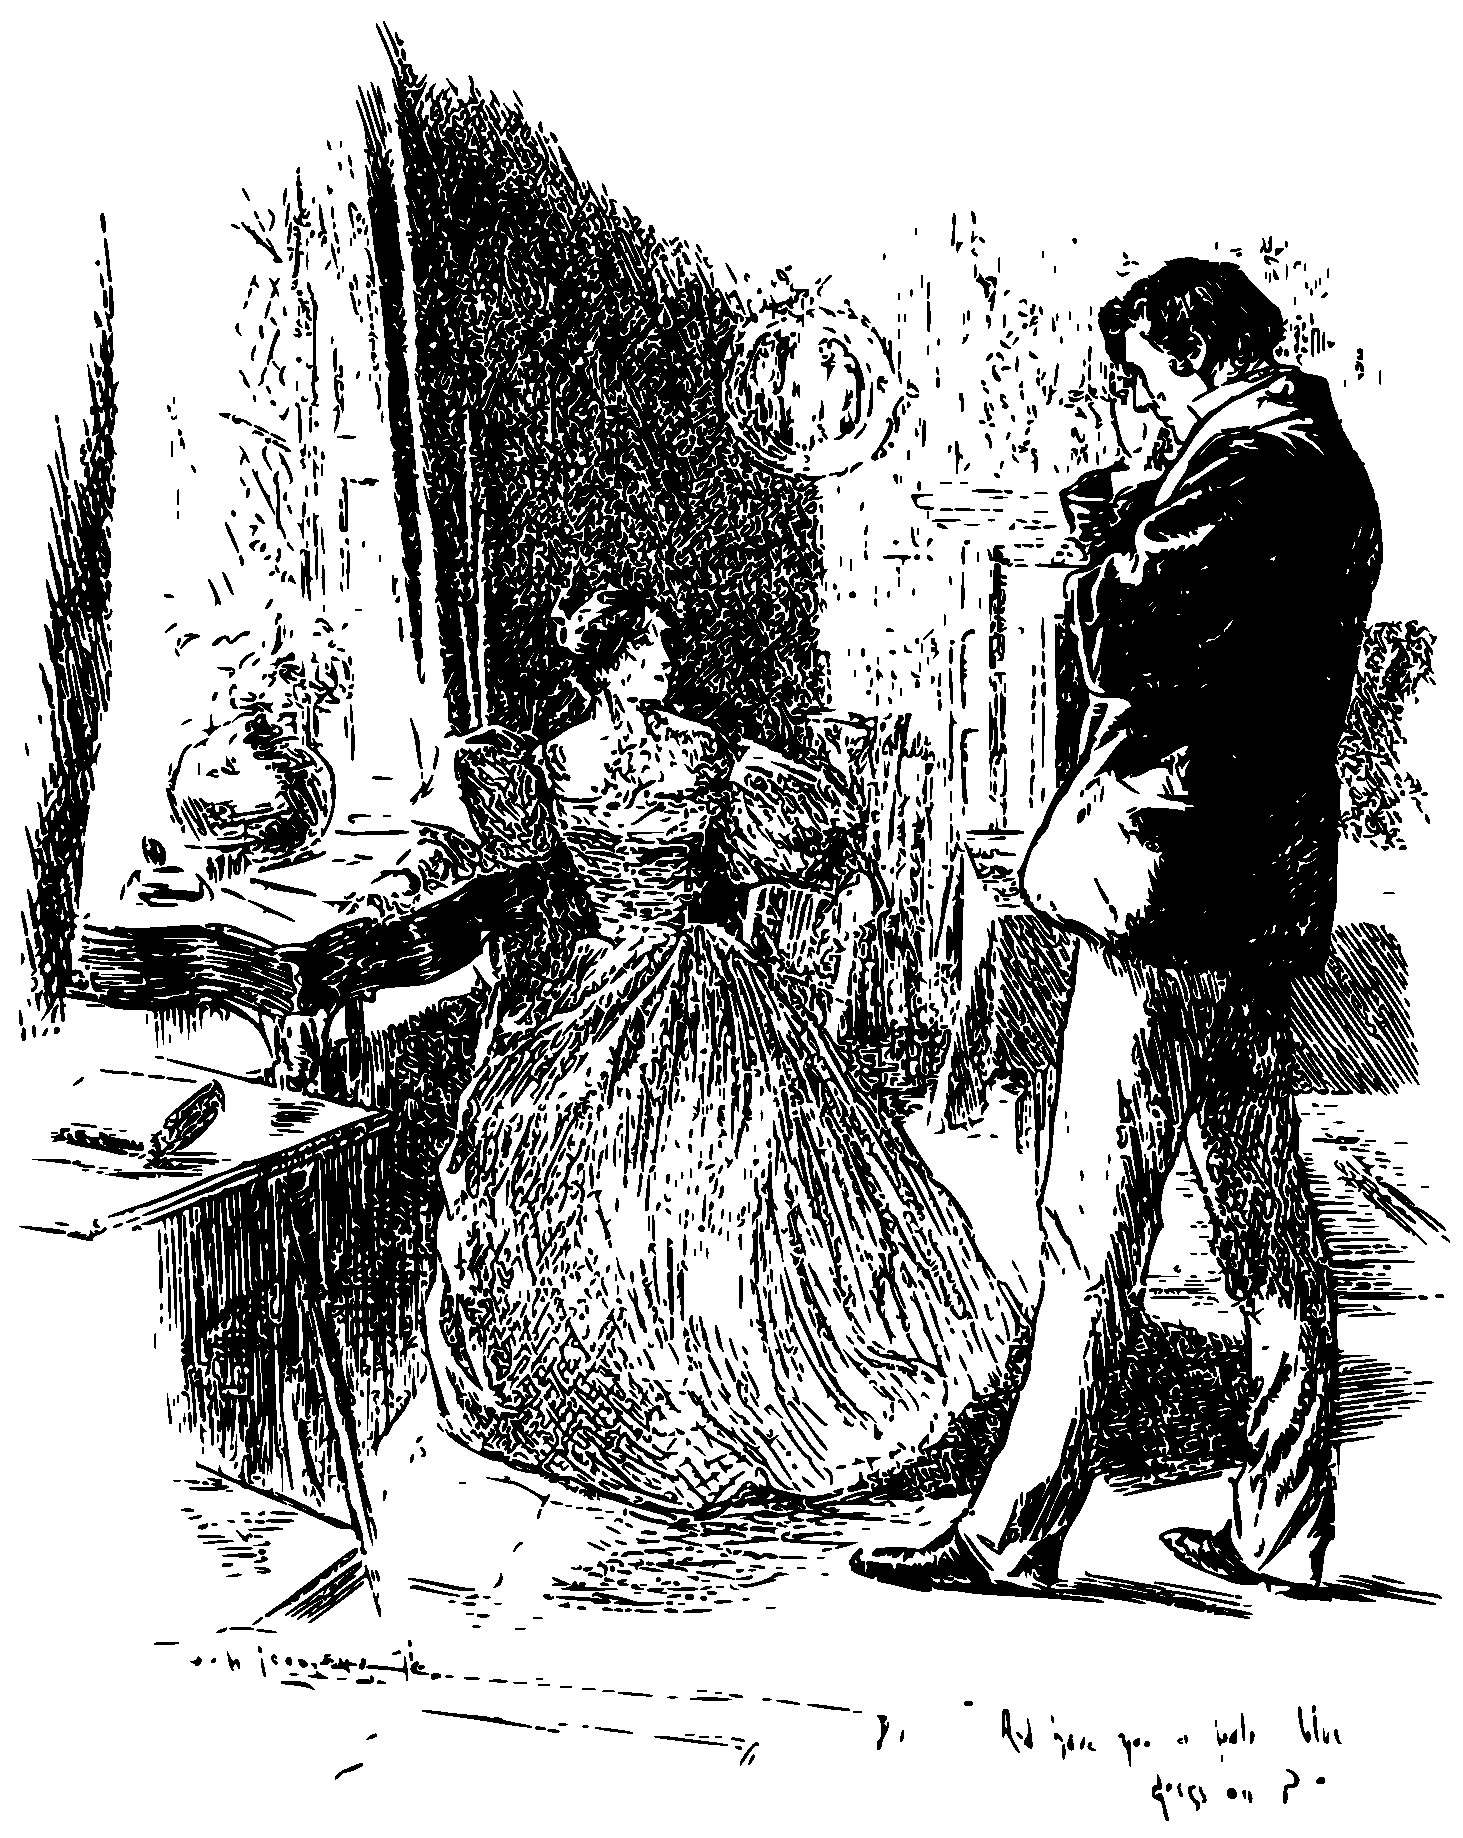
\includegraphics[width=\linewidth]{images/p435b.pdf}
	\end{sidecaption}
\end{figure}

I had. He informed me then, that for some time he had fancied the
obscurity clouding one eye was becoming less dense; and that now he was
sure of it.

He and I went up to London. He had the advice of an eminent oculist;
and he eventually recovered the sight of that one eye. He cannot now
see very distinctly: he cannot read or write much; but he can find his
way without being led by the hand: the sky is no longer a blank to
him---the earth no longer a void. When his first-born was put into his
arms, he could see that the boy had inherited his own eyes, as they once
were---large, brilliant, and black. On that occasion, he again, with a
full heart, acknowledged that God had tempered judgment with mercy.

My Edward and I, then, are happy: and the more so, because those we most
love are happy likewise. Diana and Mary Rivers are both married:
alternately, once every year, they come to see us, and we go to see
them. Diana's husband is a captain in the navy, a gallant officer and a
good man. Mary's is a clergyman, a college friend of her brother's,
and, from his attainments and principles, worthy of the connection.
Both Captain Fitzjames and \Mr{} Wharton love their wives, and are loved
by them.

As to \St{} John Rivers, he left England: he went to India. He entered on
the path he had marked for himself; he pursues it still. A more
resolute, indefatigable pioneer never wrought amidst rocks and dangers.
Firm, faithful, and devoted, full of energy, and zeal, and truth, he
labours for his race; he clears their painful way to improvement; he
hews down like a giant the prejudices of creed and caste that encumber
it. He may be stern; he may be exacting; he may be ambitious yet; but
his is the sternness of the warrior Greatheart, who guards his pilgrim
convoy from the onslaught of Apollyon. His is the exaction of the
apostle, who speaks but for Christ, when he says---\enquote{Whosoever
	will come after me, let him deny himself, and take up his cross and
	follow me.} His is the ambition of the high master-spirit, which aims
to fill a place in the first rank of those who are redeemed from the
earth---who stand without fault before the throne of God, who share the
last mighty victories of the Lamb, who are called, and chosen, and
faithful.

\St{} John is unmarried: he never will marry now. Himself has hitherto
sufficed to the toil, and the toil draws near its close: his glorious
sun hastens to its setting. The last letter I received from him drew
from my eyes human tears, and yet filled my heart with divine joy: he
anticipated his sure reward, his incorruptible crown. I know that a
stranger's hand will write to me next, to say that the good and faithful
servant has been called at length into the joy of his Lord. And why
weep for this? No fear of death will darken \St{} John's last hour: his
mind will be unclouded, his heart will be undaunted, his hope will be
sure, his faith steadfast. His own words are a pledge of this---

\enquote{My Master,} he says, \enquote{has forewarned me. Daily He
	announces more distinctly,---\enquote{Surely I come quickly!} and hourly I more
	eagerly respond,---\enquote{Amen; even so come, Lord Jesus!}}


\clearpage

%\begin{vplace}
%\begin{center}
%	\includegraphics[width=5cm]{symbols/bird_1.pdf}
%\end{center}
%\end{vplace}

\appendix
\backmatter

% Print info
\settypeoutlayoutunit{mm}
\typeoutlayout
\typeoutstandardlayout

\end{document}
